% Author: Alfredo Sánchez Alberca (asalber@ceu.es)
%----------------------------------------------------------------------------------------
%    DOCUMENT CLASS
%----------------------------------------------------------------------------------------

\documentclass[11pt,openright]{book}
%----------------------------------------------------------------------------------------
%	PACKAGES AND OTHER DOCUMENT CONFIGURATIONS
%----------------------------------------------------------------------------------------

% Encoding settings
\usepackage[utf8]{inputenc}

% Language settings
\usepackage[spanish]{babel}

% Margins and layout
\usepackage[top=3cm, bottom=3cm, left=2.54cm, right=2.54cm]{geometry}

% Font settings
\usepackage{type1cm}

% Math support
\usepackage{amsmath}

% Line breaking
\usepackage{microtype} 
\setlength{\emergencystretch}{2em}

% Graphics
\usepackage{graphicx}

% Arrays and tables
\usepackage{array}
\usepackage{multirow}

% Captions
\usepackage[margin=10mm,font=footnotesize,labelfont=bf]{caption}

% Pstricks
\usepackage[usenames,dvipsnames]{pstricks} % Postscript graphics
\usepackage{pst-all,pstricks-add,pst-math,pst-plot,pst-infixplot,pst-xkey}
\usepackage{epsfig}

% Floating figures
\usepackage{subfigure}

% Lists
\usepackage[shortlabels]{enumitem} % Customize lists
%\setlist{nolistsep} % Reduce spacing between bullet points and numbered lists
\setlist[description]{style=sameline,leftmargin=0cm}

\makeatletter
\let\savees@listquot\es@listquot
\def\es@listquot{\protect\savees@listquot}
\makeatletter

\renewcommand{\theenumiii}{\arabic{enumiii}}

% Bibliography
%\usepackage[style=alphabetic,sorting=nyt,sortcites=true,autopunct=true,babel=hyphen,hyperref=true,abbreviate=false,backref=true,backend=biber]{biblatex}
%\addbibresource{bibliography.bib} % BibTeX bibliography file
%\defbibheading{bibempty}{}

% Flush floating 
\usepackage{afterpage}


% hyperlinks
\usepackage[pdfauthor={Alfredo Sánchez Alberca}, pdftitle={Bioestadistica aplicada con R y RKTeaching},breaklinks,colorlinks=true]{hyperref}
\usepackage{breakurl}

% Indentation
%\setlength\parindent{0pt}

% Control of widow orphan lines
\clubpenalty=10000
\widowpenalty=10000 


% Caption formatting
\usepackage[margin=20pt, font=small, labelfont=bf, labelsep=endash]{caption}

% Code listing formatting
\usepackage{listings}
\lstdefinelanguage{morejava}{morekeywords={String}}
\definecolor{vollgrau}{rgb}{0.9,0.9,0.9}
\definecolor{colKeys}{rgb}{0,0,1}
\definecolor{colIdentifier}{rgb}{0,0,0}
\definecolor{colComments}{rgb}{1,0.5,0}
\definecolor{colString}{rgb}{0,0.5,0}
\definecolor{colbackground}{rgb}{0.9,0.9,1}
\lstset{%
     language=R,
     float=hbp,%
     basicstyle=\ttfamily,%
     identifierstyle=\color{colIdentifier},%
     keywordstyle=\color{colKeys},%
     stringstyle=\color{colString},%ROMERO OTERO, JAVIER
     commentstyle=\color{colComments},%
%    columns=flexible,%
%    columns=fullflexible,%
     columns=fixed,
     tabsize=1,%
     extendedchars=true,%
     showspaces=false,%
     showstringspaces=false,%
     breaklines=true,%
     breakindent=10pt,%
     backgroundcolor=\color{colbackground},%
     breakautoindent=true,%
     captionpos=t,%.
     xleftmargin=1em,%
%    xrightmargin=.5\fboxsep,%
     numbersep=1em,%
     escapechar=\#
}

%Indicar corto o largo según se quiera la versión corta o larga de las prácticas.
\usepackage[largo]{optional}

% Color
\usepackage{xcolor} % Required for specifying colors by name
\definecolor{ocre}{RGB}{243,102,25} % Define the orange color used for highlighting throughout the book
\definecolor{blueceu}{RGB}{5,161,230} % Blue color of CEU logo
\definecolor{greenceu}{RGB}{185,209,16} % Green color of CEU logo
\definecolor{redceu}{RGB}{137,28,36} % Red color of CEU logo
\definecolor{grayceu}{RGB}{111,107,83} % Gray color of CEU logo
\definecolor{coral}{rgb}{1,0.5,0.31} % Orange color for graphics
\definecolor{royalblue1}{rgb}{0.28,0.46,1} % Blue color for graphics
\definecolor{mygreen}{rgb}{0,0.8,0} % Grtype filter texteen color for graphics

%----------------------------------------------------------------------------------------
%	VARIOUS REQUIRED PACKAGES
%----------------------------------------------------------------------------------------

\usepackage{tikz} % Required for drawing custom shapes
%\usepackage{booktabs} % Required for nicer horizontal rules in tables
%\usepackage{eso-pic} % Required for specifying an image background in the title page

%----------------------------------------------------------------------------------------
%	SECTIONS AND SUBSECTIONS
%----------------------------------------------------------------------------------------
%\titleformat*{\section}{\Huge}
%\titleformat*{\subsection}{\Large}


% Chapter and section formatting 
\usepackage[rigidchapters,explicit]{titlesec}
\setlength{\fboxsep}{5pt}
\newlength{\titulolength}
\setlength{\titulolength}{\textwidth} 
\addtolength{\titulolength}{-2\fboxsep}
\addtolength{\titulolength}{-2\fboxrule}
\titleformat{\chapter}[display]
{\bfseries\sffamily}
{\filleft \mdseries \slshape \LARGE Práctica de Bioestadística con R y RKTeaching \Huge\thechapter}
{0.5ex}
{\colorbox{RoyalBlue}{\parbox[t]{\titulolength}{\rule{0mm}{10mm}\Huge\sffamily\filleft\textcolor{white}{#1}}}}
\titleformat{\section}{\normalfont\Large\bfseries}{\arabic{section}}{1em}{#1}
\titleformat{\subsection}{\normalfont\large\bfseries}{\arabic{section}.\arabic{subsection}}{1em}{#1}
\titleformat{\subsubsection}{\normalfont\normalsize\bfseries}{\arabic{section}.\arabic{subsection}.\arabic{subsubsection}}{0.5em}{#1}
\titlespacing{\chapter}{0pt}{0pt}{30ex}
\titlespacing{\section}{0pt}{8ex}{4ex}

%----------------------------------------------------------------------------------------
%	MAIN TABLE OF CONTENTS
%----------------------------------------------------------------------------------------

% \usepackage{titletoc} % Required for manipulating the table of contents
% 
% \contentsmargin{0cm} % Removes the default margin
% % Chapter text styling
% \titlecontents{chapter}[1.25cm] % Indentation
% {\addvspace{15pt}\large\bfseries} % Spacing and font options for chapters
% {\color{gray}\contentslabel[\Large\thecontentslabel.]{1.25cm}} % Chapter number
% {}  
% {\color{gray}\bfseries\hfill\thecontentspage} % Page number
% % Section text styling
% \titlecontents{section}[1.25cm] % Indentation
% {\addvspace{5pt}\bfseries} % Spacing and font options for sections
% {\contentslabel[\thecontentslabel]{1.25cm}} % Section number
% {}
% {\hfill\color{black}\thecontentspage} % Page number
% []
% % Subsection text styling
% \titlecontents{subsection}[1.25cm] % Indentation
% {\addvspace{1pt}\small} % Spacing and font options for subsections
% {\contentslabel[\thecontentslabel]{1.25cm}} % Subsection number
% {}
% {\;\titlerule*[.5pc]{.}\;\thecontentspage} % Page number
% [] 

%----------------------------------------------------------------------------------------
%	MINI TABLE OF CONTENTS IN CHAPTER HEADS
%----------------------------------------------------------------------------------------

% % Section text styling
% \titlecontents{lsection}[0em] % Indendating
% {\footnotesize\sffamily} % Font settings
% {}
% {}
% {}
% 
% % Subsection text styling
% \titlecontents{lsubsection}[.5em] % Indentation
% {\normalfont\footnotesize\sffamily} % Font settings
% {}
% {}
% {}
 
%----------------------------------------------------------------------------------------
%	PAGE HEADERS
%----------------------------------------------------------------------------------------

% Headings and footers
\usepackage{fancyhdr}
\pagestyle{fancy}
\fancyhead{}
\renewcommand{\chaptermark}[1]{\markboth{\thechapter.\ #1}{}}
\fancyhead[RE,LO]{\scshape Bioestadística Aplicada con R y RKTeaching}
\fancyhead[LE,RO]{\sffamily\slshape \leftmark}
\renewcommand{\headrulewidth}{0pt}
\renewcommand{\floatpagefraction}{.8}
\renewcommand{\textfraction}{.1} 


% \usepackage{fancyhdr} % Required for header and footer configuration
% 
% \pagestyle{fancy}
% \renewcommand{\chaptermark}[1]{\markboth{\color{grayceu}\sffamily\normalsize\textit{#1}}{}} % Chapter text font
% % settings
% %\renewcommand{\sectionmark}[1]{\markright{\color{grayceu}\sffamily\normalsize\textit{\thesection\hspace{5pt}#1}}{}} %
% % Section text font settings
% \fancyhf{} \fancyfoot[LE,RO]{\normalsize\thepage} % Font setting for the page number in the footer
% \fancyhead[RE]{{\color{grayceu}\sffamily\normalsize\textit{Pr�cticas de Bioestad�stica con R y RKTeaching}}} % Print the nearest
% % section name on the left side of odd pages
% \fancyhead[LO]{\leftmark} % Print the current chapter name on the right side of even pages
% \renewcommand{\headrulewidth}{0pt} % Removes the rule in the header
% \addtolength{\headheight}{2.5pt} % Increase the spacing around the header slightly
% \renewcommand{\footrulewidth}{0pt} % Removes the rule in the footer
% \fancypagestyle{plain}{\fancyhead{}\renewcommand{\headrulewidth}{0pt}} % Style for when a plain pagestyle is specified
% 
% % Removes the header from odd empty pages at the end of chapters
% \makeatletter
% \renewcommand{\cleardoublepage}{
% \clearpage\ifodd\c@page\else
% \hbox{}
% \vspace*{\fill}
% \thispagestyle{empty}
% \newpage
% \fi}


%----------------------------------------------------------------------------------------
%	THEOREM STYLES
%----------------------------------------------------------------------------------------

\usepackage{amsthm} % For including math equations, theorems, symbols, etc

\newcommand{\intoo}[2]{\mathopen{]}#1\,;#2\mathclose{[}}
\newcommand{\ud}{\mathop{\mathrm{{}d}}\mathopen{}}
\newcommand{\intff}[2]{\mathopen{[}#1\,;#2\mathclose{]}}
\newtheorem{notation}{Notation}[chapter]

\newtheoremstyle{ocrenum} % Theorem style name
{7pt} % Space above
{7pt} % Space below
{\normalfont} % Body font
{} % Indent amount
{\small\bf\sffamily\color{ocre}} % Theorem head font
{\;\;} % Punctuation after theorem head
{0.25em} % Space after theorem head
{\small\sffamily\color{ocre}\thmname{#1}\thmnumber{\@ifnotempty{#1}{ }\@upn{#2}} % Theorem text (e.g. Theorem 2.1)
\thmnote{\ {\the\thm@notefont\sffamily\bfseries\color{black}--- #3.}}} % Optional theorem note
\renewcommand{\qedsymbol}{$\blacksquare$} % Optional qed square

\newtheoremstyle{blacknumex} % Theorem style name
{7pt} % Space above
{7pt} % Space below
{\normalfont} % Body font
{} % Indent amount
{\small\bf\sffamily} % Theorem head font
{\;\;} % Punctuation after theorem head
{0.25em} % Space after theorem head
{\small\sffamily{\tiny\ensuremath{\blacksquare}}\ \thmname{#1}\thmnumber{\@ifnotempty{#1}{ }\@upn{#2}} % Theorem text (e.g. Theorem 2.1)
\thmnote{\ {\the\thm@notefont\sffamily\bfseries--- #3.}}} % Optional theorem note

\newtheoremstyle{blacknum} % Theorem style name
{7pt} % Space above
{7pt} % Space below
{\normalfont} % Body font
{} % Indent amount
{\small\bf\sffamily} % Theorem head font
{\;\;} % Punctuation after theorem head
{0.25em} % Space after theorem head
{\small\sffamily\thmname{#1}\thmnumber{\@ifnotempty{#1}{ }\@upn{#2}} % Theorem text (e.g. Theorem 2.1)
\thmnote{\ {\the\thm@notefont\sffamily\bfseries--- #3.}}} % Optional theorem note

\newtheoremstyle{example} % Theorem style name
{7pt} % Space above
{7pt} % Space below
{\normalfont} % Body font
{} % Indent amount
{\small\bf\sffamily} % Theorem head font
{\;\;} % Punctuation after theorem head
{0.25em} % Space after theorem head
{\small\sffamily\thmname{#1} % Theorem text (e.g. Theorem 2.1)
\thmnote{\ {\the\thm@notefont\sffamily\bfseries--- #3.}}} % Optional theorem note

\newtheoremstyle{indication} % Theorem style name
{-5pt} % Space above
{7pt} % Space below
{\normalfont} % Body font
{-28pt} % Indent amount
{\bf} % Theorem head font
{\kern-11.5pt} % Punctuation after theorem head
{20pt} % Space after theorem head
{\begin{tikzpicture}
\draw[anchor=west] (-26pt,10pt) node [fill=gray,opacity=1,inner
sep=1pt]{\Large\bfseries\textcolor{white}{\vphantom{plPQq}\makebox[17pt][c]{\emph{i}}}}; \end{tikzpicture}} % Theorem text (e.g. Theorem 2.1)

\makeatother

% Defines the theorem text style for each type of theorem to one of the three styles above
\theoremstyle{ocrenum}
\newtheorem{teorema}{Teorema}[chapter]
\newtheorem{proposicion}{Proposición}[chapter]
\newtheorem{problema}{Problema}[chapter]
\newtheorem{ejercicio}{Ejercicio}[chapter]
\theoremstyle{blacknumex}
\newtheorem{ejemplo}{Ejemplo}[chapter]
\theoremstyle{blacknum}
\newtheorem{vocabulario}{Vocabulario}[chapter]
\newtheorem{definicion}{Definición}[chapter]
\newtheorem{corolario}{Corolario}[chapter]
\theoremstyle{indication}
\newtheorem{indicacionT}{Indicación}
%\theoremstyle{example}
%\newtheorem{ejemplo}{Ejemplo}

%----------------------------------------------------------------------------------------
%	DEFINITION OF COLORED BOXES
%----------------------------------------------------------------------------------------

\RequirePackage[framemethod=default]{mdframed} % Required for creating the theorem, definition, exercise and corollary boxes

% Theorem box
\newmdenv[skipabove=7pt,
skipbelow=7pt,
backgroundcolor=black!5,
linecolor=ocre,
innerleftmargin=5pt,
innerrightmargin=5pt,
innertopmargin=5pt,
leftmargin=0cm,
rightmargin=0cm,
innerbottommargin=5pt]{tBox}

% Exercise box	  
\newmdenv[skipabove=7pt,
skipbelow=7pt,
rightline=false,
leftline=true,
topline=false,
bottomline=false,
backgroundcolor=ocre!10,
linecolor=ocre,
innerleftmargin=5pt,
innerrightmargin=5pt,
innertopmargin=5pt,
innerbottommargin=5pt,
leftmargin=0cm,
rightmargin=0cm,
linewidth=4pt]{eBox}	

% Definition box
\newmdenv[skipabove=10pt,
skipbelow=10pt,
rightline=false,
leftline=true,
topline=false,
bottomline=false,
linecolor=ocre,
innerleftmargin=5pt,
innerrightmargin=5pt,
innertopmargin=0pt,
leftmargin=0cm,
rightmargin=0cm,
linewidth=4pt,
innerbottommargin=0pt]{dBox}	

% Corollary box
\newmdenv[skipabove=7pt,
skipbelow=7pt,
rightline=false,
leftline=true,
topline=false,
bottomline=false,
linecolor=gray,
backgroundcolor=black!5,
innerleftmargin=5pt,
innerrightmargin=5pt,
innertopmargin=5pt,
leftmargin=0cm,
rightmargin=0cm,
linewidth=4pt,
innerbottommargin=5pt]{cBox}	

% Indication box
\newmdenv[skipabove=7pt,
skipbelow=7pt,
rightline=false,
leftline=true,
topline=false,
bottomline=false,
linecolor=gray,
backgroundcolor=black!5,
innerleftmargin=5pt,
innerrightmargin=5pt,
innertopmargin=5pt,
leftmargin=0pt,
rightmargin=0pt,
linewidth=4pt,
innerbottommargin=5pt]{iBox}				  
		  			  


% Creates an environment for each type of theorem and assigns it a theorem text style from the "Theorem Styles" section above and a colored box from above
\newenvironment{theorem}{\begin{tBox}\begin{theoremeT}}{\end{theoremeT}\end{tBox}}
\newenvironment{exercise}{\begin{eBox}\begin{exerciseT}}{\hfill{\color{ocre}\tiny\ensuremath{\blacksquare}}\end{exerciseT}\end{eBox}}				  
\newenvironment{definition}{\begin{dBox}\begin{definitionT}}{\end{definitionT}\end{dBox}}	
\newenvironment{example}{\begin{exampleT}}{\hfill{\tiny\ensuremath{\blacksquare}}\end{exampleT}}		
\newenvironment{corollary}{\begin{cBox}\begin{corollaryT}}{\end{corollaryT}\end{cBox}}	
\newenvironment{indicacion}{\begin{iBox}\begin{indicacionT}}{\end{indicacionT}\end{iBox}}	

%----------------------------------------------------------------------------------------
%	REMARK ENVIRONMENT
%----------------------------------------------------------------------------------------

%\newenvironment{remark}{\par\vskip10pt\small % Vertical white space above the remark and smaller font size
%\begin{list}{}{
%\leftmargin=35pt % Indentation on the left
%\rightmargin=25pt}\item\ignorespaces % Indentation on the right
%\makebox[-2.5pt]{\begin{tikzpicture}[overlay]
%\node[draw=ocre!60,line width=1pt,circle,fill=ocre!25,font=\sffamily\bfseries,inner sep=2pt,outer sep=0pt] at (-15pt,0pt){\textcolor{ocre}{R}};\end{tikzpicture}} % Orange R in a circle
%\advance\baselineskip -1pt}{\end{list}\vskip5pt} % Tighter line spacing and white space after remark

% %----------------------------------------------------------------------------------------
% %	SECTION NUMBERING IN THE MARGIN
% %----------------------------------------------------------------------------------------
% 
% \makeatletter
% %\renewcommand{\@seccntformat}[1]{\llap{\textcolor{grayceu}{\csname the#1\endcsname.}\hspace{1em}}}                    
% \renewcommand{\section}{
% 	\@startsection{section}{1}{\z@}
% 	{-4ex \@plus -1ex \@minus -.4ex}{1ex \@plus.2ex }
% 	{\normalfont\LARGE}
% }
% \renewcommand{\subsection}{
% 	\@startsection{subsection}{2}{\z@}
% 	{-3ex \@plus -0.1ex \@minus -.4ex}{0.5ex \@plus.2ex }
% 	{\normalfont\Large}
% }
% \renewcommand{\subsubsection}{
% 	\@startsection{subsubsection}{3}{\z@}
% 	{-2ex \@plus -0.1ex \@minus -.2ex}{0.2ex \@plus.2ex }
% 	{\normalfont\large}
% }                        
% \renewcommand{\paragraph}{
% 	\@startsection{paragraph}{4}{\z@}
% 	{-2ex \@plus-.2ex \@minus .2ex}{0.1ex}
% 	{\normalfont\bfseries}
% }
% 
% \def\thechapter{\arabic{chapter}}
% \def\thesection{\thechapter.\arabic{section}.}
% \def\thesubsection{\thesection\arabic{subsection}.}
% \def\thesubsubsection{\thesubsection\arabic{section}.}
% 
% %----------------------------------------------------------------------------------------
% %	CHAPTER HEADINGS
% %----------------------------------------------------------------------------------------
% %\newcommand{\thechapterimage}{}
% %\newcommand{\chapterimage}[1]{\renewcommand{\thechapterimage}{#1}}
% \def\@makechapterhead#1{
% \thispagestyle{empty}
% {
% \ifnum \c@secnumdepth >\m@ne
% \if@mainmatter
% \startcontents
% \begin{tikzpicture}[remember picture,overlay]
% % \node at (current page.north west)
% % {\begin{tikzpicture}[remember picture,overlay]
% % 
% % %\node[anchor=north west] at (-4pt,-27.5mm) {\includegraphics[width=\paperwidth]{\thechapterimage}};
% % %Commenting the 3 lines below removes the small contents box in the chapter heading
% % % \draw[fill=white,opacity=.6] (30mm,-30mm) rectangle (9cm,-9cm);
% % % \node[anchor=north west] at (30mm,-30mm) {\parbox[t][9cm][t]{5.5cm}{\huge\bfseries\flushleft \printcontents{l}{1}{\setcounter{tocdepth}{2}}}};
% % % \draw[anchor=west] (5cm,-11cm) node [rounded corners=25pt,fill=white,opacity=.7,inner sep=15.5pt]{\huge\sffamily\bfseries\textcolor{black}{\vphantom{plPQq}\makebox[20cm]{}}};
% \draw[anchor=north west, fill=black] (0mm,50mm) rectangle (1pt,10mm);
% \draw[anchor=north west] (0cm,20mm) node {\scalebox{1.5}{\Huge{\textcolor{grayceu}\thechapter}}}; 
% %\draw[anchor=west] (0cm,0cm) node {\Huge{#1}}; 
% \end{tikzpicture}
% \par\vspace*{2cm}
% {\Huge #1}
% \par\vspace*{1cm}
% % \end{tikzpicture}}\par\vspace*{230\p@}
% }}
% \def\@makeschapterhead#1{
% \thispagestyle{empty}
% {
% \ifnum \c@secnumdepth >\m@ne
% \if@mainmatter
% \startcontents
% \begin{tikzpicture}[remember picture,overlay]
% % \node at (current page.north west)
% % {\begin{tikzpicture}[remember picture,overlay]
% % \node[anchor=north west] at (-4pt,-27.5mm) {\includegraphics[width=\paperwidth]{\thechapterimage}};
% % \draw[anchor=west] (5cm,-11cm) node [rounded corners=25pt,fill=white,opacity=.7,inner sep=15.5pt]{\huge\sffamily\bfseries\textcolor{black}{\vphantom{plPQq}\makebox[20cm]{}}};
% % \draw[anchor=west] (5cm,-11cm) node [rounded corners=25pt,inner sep=15.5pt]{\huge\sffamily\bfseries\textcolor{black}{#1\vphantom{plPQq}\makebox[20cm]{}}};
% % \end{tikzpicture}};
% % \end{tikzpicture}}\par\vspace*{230\p@}
% %\draw[anchor=west] (0cm,0cm) node {\Huge{#1}}; 
% \end{tikzpicture}
% {\Huge #1}
% \par\vspace*{1cm}
% }}
% \makeatother

 % Insert the commands_book.tex file which contains the majority of the structure behind the template

%----------------------------------------------------------------------------------------
%	COMMANDS FOR INDICATIONS
%----------------------------------------------------------------------------------------
\usepackage{menukeys}
\renewmenumacro{\menu}[>]{paths}
%\newmenustylesimple*{botonstyle}{\textbf{\CurrentMenuElement}}
%\renewmenumacro{\keys}{botonstyle}
\newcommand{\boton}[1]{\textsf{#1}}
\newcommand{\opcion}[1]{\textsf{#1}}
\newcommand{\campo}[1]{\textsf{#1}}
\newcommand{\comando}[1]{\texttt{#1}}
\newcommand{\variable}[1]{\textsf{#1}}
\newcommand{\resultado}[1]{\texttt{#1}}

%----------------------------------------------------------------------------------------
%	HYPHENATION
%----------------------------------------------------------------------------------------
\hyphenation{fre-cuen-cias, pro-ba-bi-li-dad, pro-ba-bi-li-da-des, Fre-cuen-cias, Pro-ba-bi-li-dad, Pro-ba-bi-li-da-des}


% OTHERS
\newcommand{\resetcounters}{\setcounter{page}{1} \setcounter{section}{0} \setcounter{footnote}{0} \setcounter{figure}{0} \setcounter{table}{0}}




%========================================================================================
%   DOCUMENT BODY
%========================================================================================
\begin{document}
\frontmatter 
% Add two blank pages at the begining
%\null\thispagestyle{empty}\newpage
%\null\thispagestyle{empty}\newpage
%----------------------------------------------------------------------------------------
%	TITLE PAGE
%----------------------------------------------------------------------------------------
\begin{titlepage}
% \AddToShipoutPictureBG*{
\includegraphics[width=\paperwidth,height=\paperheight]{img/portada}}
% \clearpage
% \thispagestyle{empty}
% \end{titlepage}
% 
% \null\newpage
% \thispagestyle{empty}
% 
% \null\newpage
\thispagestyle{empty}
%\thispagestyle{empty}
\vspace*{7cm}
\par

% Book title
\begin{center}
\normalfont\fontsize{30}{30}\selectfont
{\bfseries \color{blueceu}Bioestadística Aplicada con R y rk.Teaching}
\end{center}
%\vspace*{5mm}
%\hrule
\vspace{1cm}
% Authors names
\begin{center}
\Large
\begin{tabular}{c}
Santiago Angulo Díaz-Parreño (\url{sangulo@ceu.es})\\
Juan Carlos Garro Garro (\url{garro.eps@ceu.es})\\
Eduardo López Ramírez (\url{elopez@ceu.es})\\
José Rojo Montijano (\url{jrojo.eps@ceu.es})\\
Anselmo Romero Limón (\url{arlimon@ceu.es})\\
Alfredo Sánchez Alberca (\url{asalber@ceu.es})\\
Susana Victoria Rodríguez (\url{victoria.eps@ceu.es})
%\url{http://aprendeconalf.es}
\end{tabular}

\medskip 
Departamento de Matemática Aplicada y Estadística\\ CEU San Pablo\\[1cm]
\medskip 
Septiembre 2016

\vspace{1cm}

\includegraphics[height=3cm]{img/logo_uspceu}
\end{center}
\vfill
\end{titlepage} 

%----------------------------------------------------------------------------------------
%	COPYRIGHT PAGE
%----------------------------------------------------------------------------------------
% Términos de la licencia Creative Commons 2.5
\begin{titlepage}
\null
\vfill
\hrule depth 3pt
\smallskip
\sffamily

\noindent \textbf{Bioestadística Aplicada con R y RKTeaching}\\
Alfredo Sánchez Alberca (asalber@gmail.com).

\bigskip
\begin{center}

\includegraphics[scale=0.1]{img/cc-logo}
\end{center}

\medskip
\small
Esta obra está bajo una licencia Reconocimiento­-No comercial-­Compartir bajo la misma licencia 2.5 España de Creative Commons. 
Para ver una copia de esta licencia, visite \url{http://creativecommons.org/licenses/by­nc­sa/2.5/es/} o envie una  
carta a Creative Commons, 171 Second Street, Suite 300, San Francisco, California  94105, USA.

\medskip
Con esta licencia eres libre de:
\begin{itemize}
\item Copiar, distribuir y mostrar este trabajo.
\item Realizar modificaciones de este trabajo.
\end{itemize}

Bajo las siguientes condiciones:
\begin{center}
\begin{tabular}{ccp{10cm}}

\includegraphics[scale=0.2]{img/cc-by} & \qquad & \textbf{Reconocimiento}. Debe reconocer los créditos de la obra de la manera especificada por el autor o el licenciador (pero no de una manera que sugiera que tiene su apoyo o apoyan el uso que hace de su obra).\\

\includegraphics[scale=0.2]{img/cc-e} & \qquad & \textbf{No comercial}. No puede utilizar esta obra para fines comerciales.\\

\includegraphics[scale=0.2]{img/cc-c} & \qquad & \textbf{Compartir bajo la misma licencia}. Si altera o transforma esta obra, o genera una obra derivada, sólo puede distribuir la obra generada bajo una licencia idéntica a ésta.
\end{tabular}
\end{center}

\begin{itemize}
\item Al reutilizar o distribuir la obra, tiene que dejar bien claro los términos de la licencia de esta obra.
\item Alguna de estas condiciones puede no aplicarse si se obtiene el permiso del titular de los derechos de autor
\item Nada en esta licencia menoscaba o restringe los derechos morales del autor.
\end{itemize}

\hrule depth 3pt
\end{titlepage}

%----------------------------------------------------------------------------------------
%	TABLE OF CONTENTS
%----------------------------------------------------------------------------------------
%\chapterimage{img/chapter_head.png} % Table of contents heading image
{\pagestyle{plain} % No headers
%\input{registro}
\tableofcontents\thispagestyle{empty}
  % Print the table of contents itself
\cleardoublepage % Forces the first chapter to start on an odd page so it's on the right
}

\mainmatter 
%----------------------------------------------------------------------------------------
%	CHAPTERS
%----------------------------------------------------------------------------------------
\chapter{Introducción a R y RKWard}

\section{Introducción}
La gran potencia de cálculo alcanzada por los ordenadores ha convertido a los mismos en poderosas herramientas al
servicio de todas aquellas disciplinas que, como la estadística, requieren manejar un gran volumen de datos.
Actualmente, prácticamente nadie se plantea hacer un estudio estadístico serio sin la ayuda de un buen programa de
análisis estadístico.

\emph{R} es un potente lenguaje de programación que incluye multitud de funciones para la representación el análisis de
datos.
Fue desarrollado por Robert Gentleman y Ross Ihaka en la Universidad de Auckland en Nueva Zelanda, aunque actualmente es
mantenido por una enorme comunidad científica en todo el mundo.

\begin{center}

\includegraphics[scale=0.5]{introduccion_r/img/Rlogo}
\end{center} 

Las ventajas de R frente a otros programas habituales de análisis de datos, como pueden ser SPSS, SAS, SPlus, Matlab o
Minitab, son múltiples:
\begin{itemize}
\item Es software libre y por tanto gratuito. Puede descargarse desde la web 
\url{http://www.r-project.org/}.
\item Es multiplataforma. Existen versiones para Windows, Macintosh, Linux y otras plataformas.
\item Está avalado y en constante desarrollo por una amplia comunidad científica que lo utiliza como estándar para el
análisis de datos.
\item Cuenta con multitud de paquetes para todo tipo de análisis estadísticos y representaciones gráficas, desde los más
habituales, hasta los más novedosos y sofisticados que no incluyen otros programas. Los paquetes están organizados y
documentados en un repositorio CRAN (Comprehensive R Archive Network) desde donde pueden descargarse libremente. En
España hay una copia de este repositorio en la web \url{http://cran.es.r-project.org/}.
\item Es programable, lo que permite que el usuario pueda crear fácilmente sus propias funciones o paquetes para
análisis de datos específicos.
\item Existen multitud de libros, manuales y tutoriales libres que permiten su aprendizaje e ilustran el análisis
estadístico de datos en distintas disciplinas científicas como las matemáticas, la física, la biología, la psicología, la medicina,
etc.
\end{itemize}

Por defecto el entorno de trabajo de R es en línea de comandos, lo que significa que los cálculos y los análisis se
relizan mediante comandos o instrucciones que el usuario teclea en una ventana de texto. No obstante, existen distintas
interfaces gráficas de usuario que facilitan su uso, sobre todo para usuarios noveles.
La interfaz gráfica que se utilizará para realizar estas prácticas será \emph{RKWard}, desarrollada por Thomas
Friedrichsmeier, junto al paquete rkTeaching especialmente desarrollado por el departamento de Matemáticas de la
Universidad San Pablo CEU para la docencia de estadística.

El objetivo de esta práctica es introducir al alumno en la utilización de este programa, enseñándole a realizar las
operaciones básicas más habituales de carga y manipulación de datos.

\section{Instalación}
\subsection{Instalación de R}
\begin{description}
\item[Linux] En la distribución Debian y cualquiera de sus derivadas (Ubuntu, Kubuntu, etc.) basta con teclear en la línea de
comandos
\begin{lstlisting}
> sudo apt-get install r-base-html r-cran-rcmdr r-cran-rodbc r-doc-html r-recommended
\end{lstlisting}
\item[Windows] Descargar de \url{http://cran.es.r-project.org/bin/windows/base/release.htm} el programa de instalación
de R, ejecutarlo y seguir las instrucciones de instalación.
\end{description}

\subsection{Instalación de la interfaz gráfica RKWard y el paquete rkTeaching}
La interfaz gráfica de usuario RKWard puede descargarse desde la web \url{http://rkward.sourceforge.net/} donde se
indican las instrucciones para instalarlo en cada plataforma.

Para Windows se recomienda seleccionar el paquete de instalación completa que incorpora R, las librerías gráficas de KDE
y el propio RKWard.

R dispone de una gran librería de paquetes que incorporan nuevas funciones y procedimientos.
En la instalación base de R vienen ya cargados los procedimientos y funciones para los análisis más comunes, pero en
ocasiones, para otros análisis será necesario cargar algún paquete adicional como por ejemplo el paquete
\variable{rkTeaching} que incorpora un nuevo menú a RKWard con la mayoría de los análisis que se realizarán en estas
prácticas.

Para instalar el paquete rk.Teaching, basta con descargarlo desde la dirección
\url{http://asalber.github.io/rkTeaching_es/}, arrancar R o RKWard y, en la consola de comandos, teclear el comando
\begin{lstlisting}
> setwd("ruta_a_descargas")
> install.packages("rk.Teaching",repos=NULL,dep=True)
\end{lstlisting}

La instalación de cualquier otro paquete se realiza con el mismo comando, cambiando el nombre del paquete por el
deseado.

En RKWard, también puede instalarse desde la ventana de R mediante el menú \menu{Preferencias>Configurar
paquetes}.
Con esto aparecerá una ventana donde se muestran los paquetes instalados localmente.
Para cargar un paquete instalado localmente basta son seleccionarlo y hacer clic sobre el botón \boton{Cargar}.
En esa misma ventana aparece una solapa \menu{Install/Update/Remove} que permite instalar nuevos paquetes desde un
repositorio de R.
Al hacer clic sobre esta solapa se abrirá una conexión a internet y aparecerá una ventana con los distintos
repositorios disponibles. Normalmente seleccionaremos en más cercano geográficamente, en nuestro caso Spain(Madrid).
Después aparecerá un lista de paquetes instalados y nuevos.
Para instalar un paquete nuevo basta con seleccionarlo y hacer clic en el botón \boton{Aceptar}.
Una vez instalado localmente, podrá cargarse como se ha indicado antes.


\section{Arranque}
Como cualquier otra aplicación de Windows, para arrancar el programa hay que hacer clic sobre la opción
correspondiente del menú \menu{Inicio>Programas>RKWard}, o bien sobre el icono de escritorio
\begin{center}
  
\includegraphics[scale=0.3]{introduccion_r/img/icono_rkward}
\end{center}

Al arrancar, aparece la ventana de bienvenida de RKWard (figura~\ref{g:rkward}).
\begin{figure}[htp]
\begin{center}
  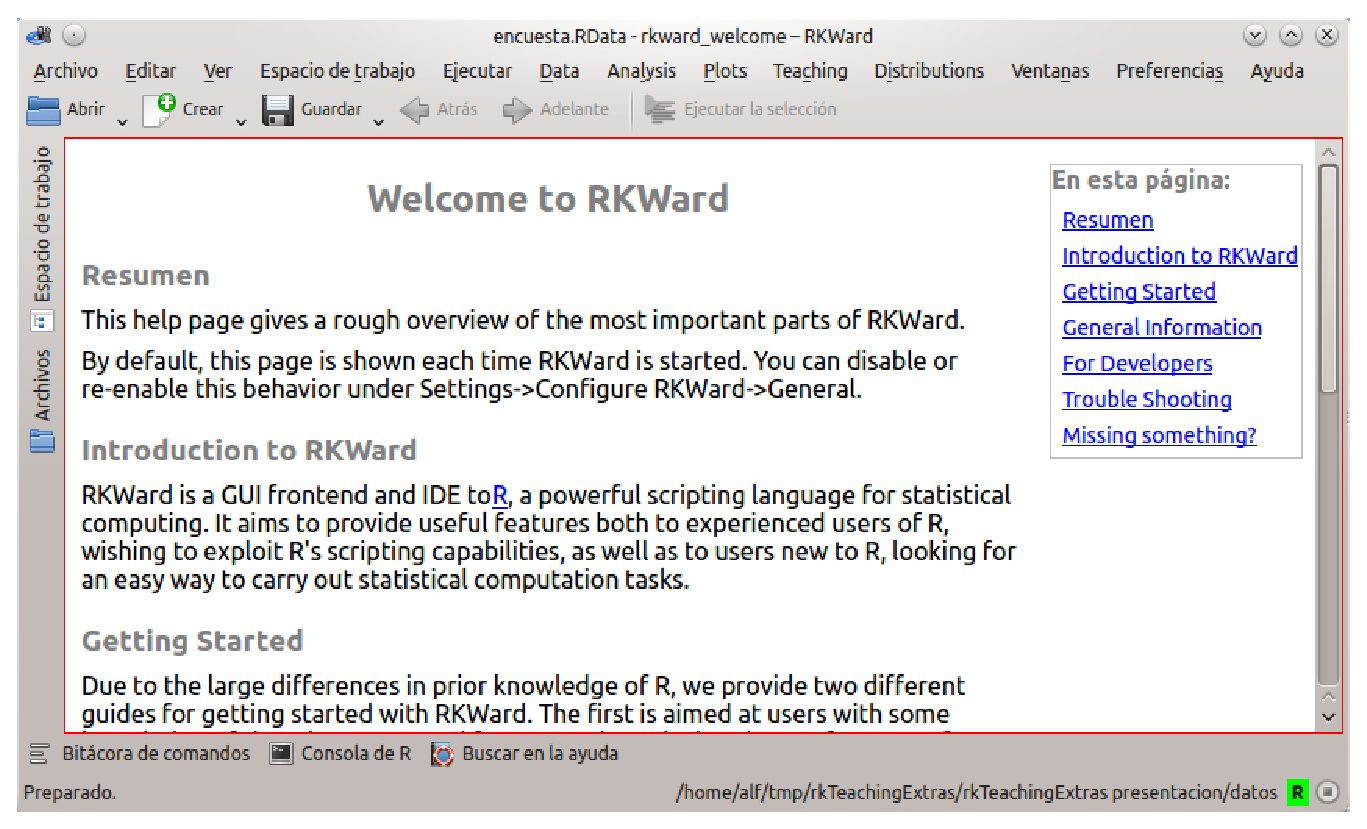
\includegraphics[scale=0.5]{introduccion_r/img/rkward}
  \caption{Interfaz gráfica de usuario de RKWard.}
  \label{g:rkward}
\end{center}
\end{figure}

La interfaz gráfica de usuario RKWard consta de los siguientes elementos:
\begin{itemize}
\item \textbf{Barra de menús}. Contiene distintos menús con operaciones que pueden realizarse con R. 
Si se ha instalado el paquete rkTeaching debe de aparecer el menú Teaching. 
\item \textbf{Barra de botones}. Contiene botones para abrir, crear y guardar conjuntos de datos, espacios de trabajo y guiones de comandos. 
\item \textbf{Ventana principal}. Es la ventana central donde apareceran la ventana de introducción de datos, los resultados de los comandos ejecutados o de las búsquedas realizadas. 
\item \textbf{Espacio de trabajo}. Es una ventana desplegable al hacer clic sobre la solapa situada en el lado izquierdo que contiene todos los elementos del espacio de trabajo de R.
Entre estos elementos aparecen los paquetes cargados, los conjuntos de datos y las variables que contienen los datos de la sesión actual. 
\item \textbf{Bitácora de comandos} Es una solapa desplegable situada en la parte inferior donde aparece un registro de todas las acciones realizadas o comandos ejecutados en la sesión de trabajo actual.
Cada vez que se seleccione un menú que lleve asociado la ejecución de algún comando, dicho comando aparecerá en esta
ventana. Esto permite modificar fácilmente los parámetros del comando y volver a ejecutarlo rápidamente sin necesidad
de volver al menú. 
\item \textbf{Consola de R} Es una solapa desplegable situada también en la parte inferior que da acceso al intérprete de comandos de R.
En esta ventana pueden teclearse y ejecutarse directamente los comandos de R.
\item \textbf{Buscar en la ayuda} Es una solapa desplegable situada en la parte inferior que permite hacer búsquedas sobre comandos de R o de algún paquete.
\item \textbf{Mensajes}. Es la línea de texto que aparece en la parte inferior, donde se muestra información adicional sobre errores, advertencias u
otra información auxiliar al ejecutar un comando, así como la ruta del espacio de trabajo activo.  
\end{itemize}

\section{Tipos de datos y operadores aritméticos y lógicos}
En R existen distintos tipos de datos. Los más básicos son:
\begin{description}
\item[Numeric]: Es cualquier número decimal. Se utiliza el punto como separador de decimales. Por defecto, cualquier
número que se teclee tomará este tipo.
\item[Integer]: Es cualquier número entero. Para convertir un número de tipo Numeric en un entero se utiliza el comando
\lstinline{as.integer()}
\item[Logical]: Puede tomar cualquiera de los dos valores lógicos \lstinline{TRUE} (verdadero) o \lstinline{FALSE}
(falso).
\item[Character]: Es cualquier cadena de caracteres alfanuméricos. Deben introducirse entre comillas. Para convertir
cualquier número en una cadena de caracteres se utiliza el comando \lstinline{as.character()}.
\end{description}

Los valores de estos tipos de datos pueden operarse utilizando distintos operadores o funciones predefinidas para cada
tipo de datos. Los más habituales son:
\begin{description}
\item[Operadores aritméticos]: \lstinline{+} (suma), \lstinline{-} (resta), \lstinline{*} (producto), \lstinline{/}
(cociente), \lstinline{^} (potencia).
\item[Operadores de comparación]: \lstinline{>} (mayor), \lstinline{<} (menor), \lstinline{>=} (mayor o igual),
\lstinline{<=} (menor o igual), \lstinline{==} (igual), \lstinline{!=} (distinto).
\item[Operadores lógicos]:  \lstinline{&} (conjunción y), \lstinline{|} (disyunción o), \lstinline{!} (negación no).
\item[Funciones predefinidas]: \lstinline{sqrt()} (raíz cuadrada), \lstinline{abs()} (valor absoluto),
\lstinline{log()} (logarítmo neperiano), \lstinline{exp()} (exponencial), \lstinline{sin()} (seno), \lstinline{cos()}
(coseno), \lstinline{tan()} (tangente).
\end{description}

Al evaluar las expresiones aritméticas existe un orden de prioridad entre los operadores de manera que primero se
evaluan las funciones predefinidas, luego las potencias, luego los productos y cocientes, luego las sumas y restas,
luego los operadores de comparación, luego las negaciones, luego las conjunciones y finalmente las disyunciones. Para
forzar un orden de evaluación distinto del predefinido se pueden usar paréntesis. Por ejemplo
\begin{lstlisting}
> 2^2+4/2
[1] 6
> (2^2+4)/2
[1] 4
> 2^(2+4/2)
[1] 16
> 2^(2+4)/2
[1] 32
> 2^((2+4)/2)
[1] 8
\end{lstlisting}

También es posible asignar valores a variables mediante el operador de asignación \lstinline{=}. Una vez definidas, las
variables pueden usarse en cualquier expresión aritmética o lógica. Por ejemplo,
\begin{lstlisting}
> x=2
> y=x+2
> y
[1] 4
> y>x
[1] TRUE
> x>=y
[1] FALSE
> x==y-2
[1] TRUE
> x!=0 & !y<x
[1] TRUE
\end{lstlisting}


\section{Introducción y manipulación de datos}
Antes de realizar cualquier análisis de datos hay que introducir los datos que se quieren analizar. 


\subsection{Introducción de datos en línea de comandos}
Existen muchas formas de introducir datos en R pero aquí sólo veremos las más habituales. La forma más rápida de
introducir datos es usar la consola de R para crear un vector de datos mediante el comando \lstinline{c()}. Por ejemplo, para introducir las notas de 5
alumnos se debe teclear en la consola de R
\begin{lstlisting}
> nota = c(5.6,7.2,3.5,8.1,6.4)
\end{lstlisting}
Esto crea el vector \variable{nota} con el que posteriormente se pueden realizar cálculos como por ejemplo la
media
\begin{lstlisting}
> mean(nota)
[1] 6.16
\end{lstlisting}

Otra forma habitual de introducir los datos de una muestra es crear un conjunto de datos mediante el comando
\lstinline{data.frame()}. Por ejemplo, para crear un conjunto de datos a partir de las notas anteriores, hay que teclear
\begin{lstlisting}
> curso = data.frame(nota)
\end{lstlisting}
Esto crea una matriz de datos en la que cada columna se corresponde con una variable y cada fila con un individuo de la
muestra. En el ejemplo la matriz \variable{curso} sólo tendría una columna que se correspondería con las notas y 5
filas, cada una de ellas correspondiente a un alumno de la muestra. Es posible acceder a las variables de un conjunto de
datos con el operador dolar \lstinline{$}. Por ejemplo, para acceder a las notas hay que teclear
\begin{lstlisting}
> curso$nota
[1] 5.6 7.2 3.5 8.1 6.4
\end{lstlisting}
Es fácil añadir nuevas variables a un conjunto de datos, pero siempre deben tener el mismo tamaño muestral. Por ejemplo,
para añadir una nueva variable con el grupo (mañana o tarde) de los alumnos, hay que teclear
\begin{lstlisting}
> curso$grupo = c("m","t","t","m","m")
\end{lstlisting}
Ahora el conjunto de datos \variable{curso} tendría dos columnas, una para la nota y otra para el grupo de los alumnos.
Tecleando el nombre de cualquier objeto, se muestra su información:
\begin{lstlisting}
> curso
   nota   grupo
1   5.6      m
2   7.2      t
3   3.5      t
4   8.1      m
5   6.4      m
\end{lstlisting}

Cuando se introducen datos se puede utilizar el código \lstinline{NA} (not available), para indicar la ausencia del
dato.

Las variables definidas en cada sesión de trabajo quedan almacenas en la memoria interna de R en lo que se conoce como
\emph{espacio de trabajo}.
Es posible obtener un listado de todos los objetos almacenados en el espacio de trabajo mediante los comandos
\lstinline{ls()}.
Si se desea más información, el comando \lstinline{ls.str()} además de mostrar los objetos de la memoria indica sus
tipos y sus valores.
\begin{lstlisting}
> ls()
[1] "curso" "nota"  "x"     "y"    
> ls.str()
curso : 'data.frame':   5 obs. of  2 variables:
 $ nota : num  5.6 7.2 3.5 8.1 6.4
 $ grupo: chr  " m " " t " " t " " m " ...
nota :  num [1:5] 5.6 7.2 3.5 8.1 6.4
x :  num 2
y :  num 4
\end{lstlisting}

Para eliminar un objeto de la memoria se utiliza el comando \lstinline{rm()}.
\begin{lstlisting}
> ls()
[1] "curso" "nota"  "x"     "y"    
> rm(x,y)
> ls()
[1] "curso" "nota"
\end{lstlisting}


\subsection{Introducción de datos en RKWard}
RKWard dispone de una interfaz gráfica para introducir los datos sin necesidad de saberse los comandos anteriores.
Para ello hay que ir al menu \menu{Archivo>Nuevo >Conjunto de datos}. Con esto
aparecerá una ventana donde hay que darle un nombre al conjunto de datos y tras esto aparece la ventana de la
figura~\ref{g:matriz_datos} con una tabla en la que se pueden introducir los datos de la muestra.
Al igual que antes, cada variable debe introducirse en una columna y cada individuo en una fila.

\begin{figure}[htp]
\begin{center}
  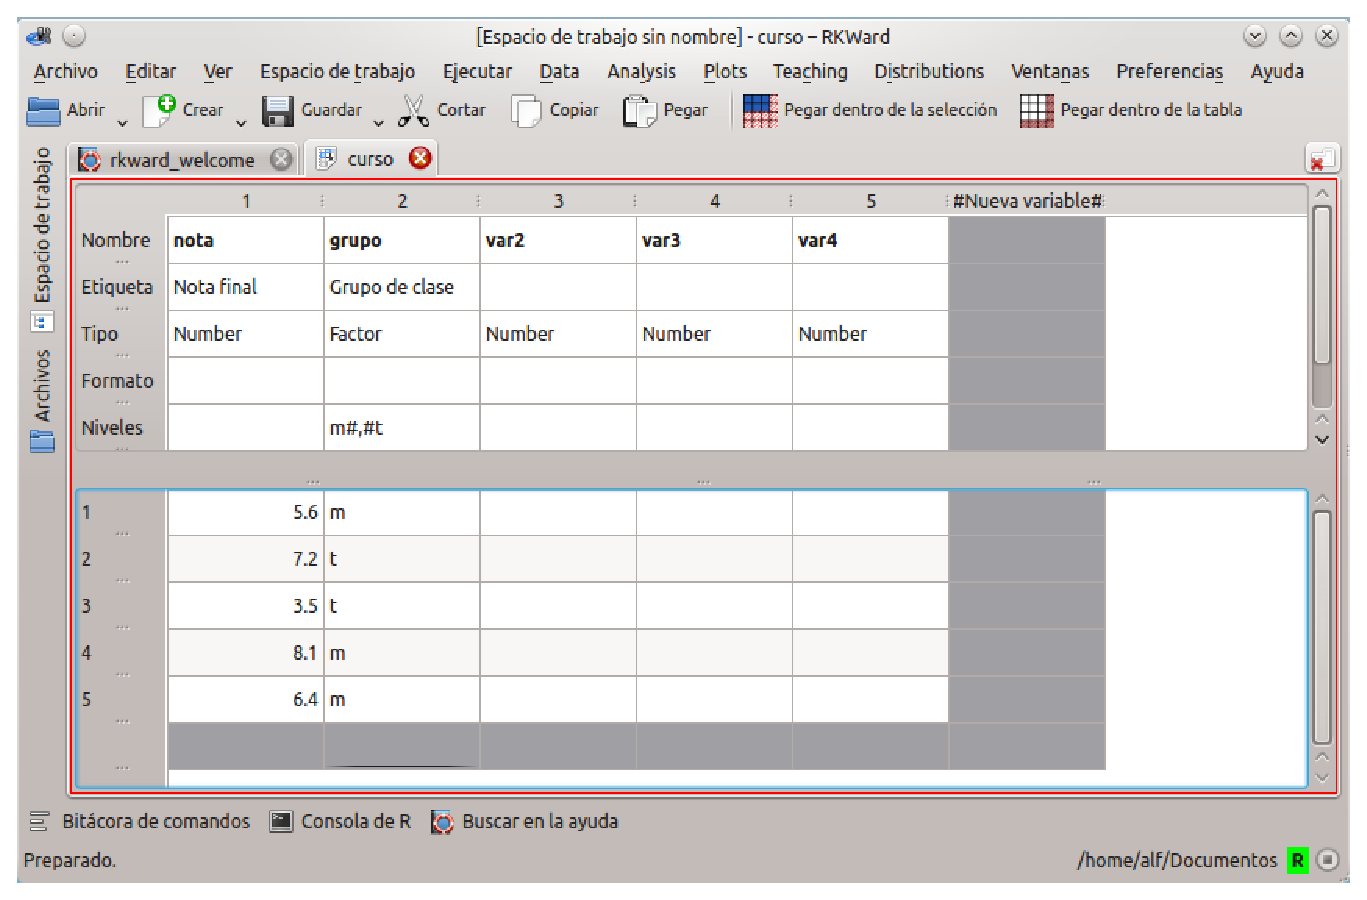
\includegraphics[scale=0.6]{introduccion_r/img/matriz_datos}
  \caption{Ventana de introducción de datos}
  \label{g:matriz_datos}
\end{center}
\end{figure}

Haciendo clic en las casillas de la cabecera cada fila es posible cambiar el nombre de la variable, ponerle una
etiqueta, su tipo, su formato y los niveles en caso de tratarse de un factor o variable categórica.
Los nombres de variables deben comenzar con una letra o un punto y pueden contener cualquier letra, punto, subrayado
(\lstinline{_}) o número.
En particular, no se pueden utilizar espacios en blanco.
Además, R es distingue entre mayúsculas y minúsculas.

Una vez definida la variable, para introducir los datos basta con teclearlos en las casillas que aparecen más abajo en
la misma columna.

R permite definir más de un conjunto de datos en un mismo espacio de trabajo.

Los objetos definidos en el espacio de trabajo pueden verse haciendo clic en la solapa \menu{Espacio de trabajo}.
Para editar una variable o un conjunto de datos basta con hacer doble clic sobre él.
También puede obtenerse un resumen como el que se muestra en la figura~\ref{g:resumen_datos} haciendo clic en el botón
derecho y seleccionando \menu{ver} en el menú contextual que aparece.

\begin{figure}[htp]
\begin{center}
  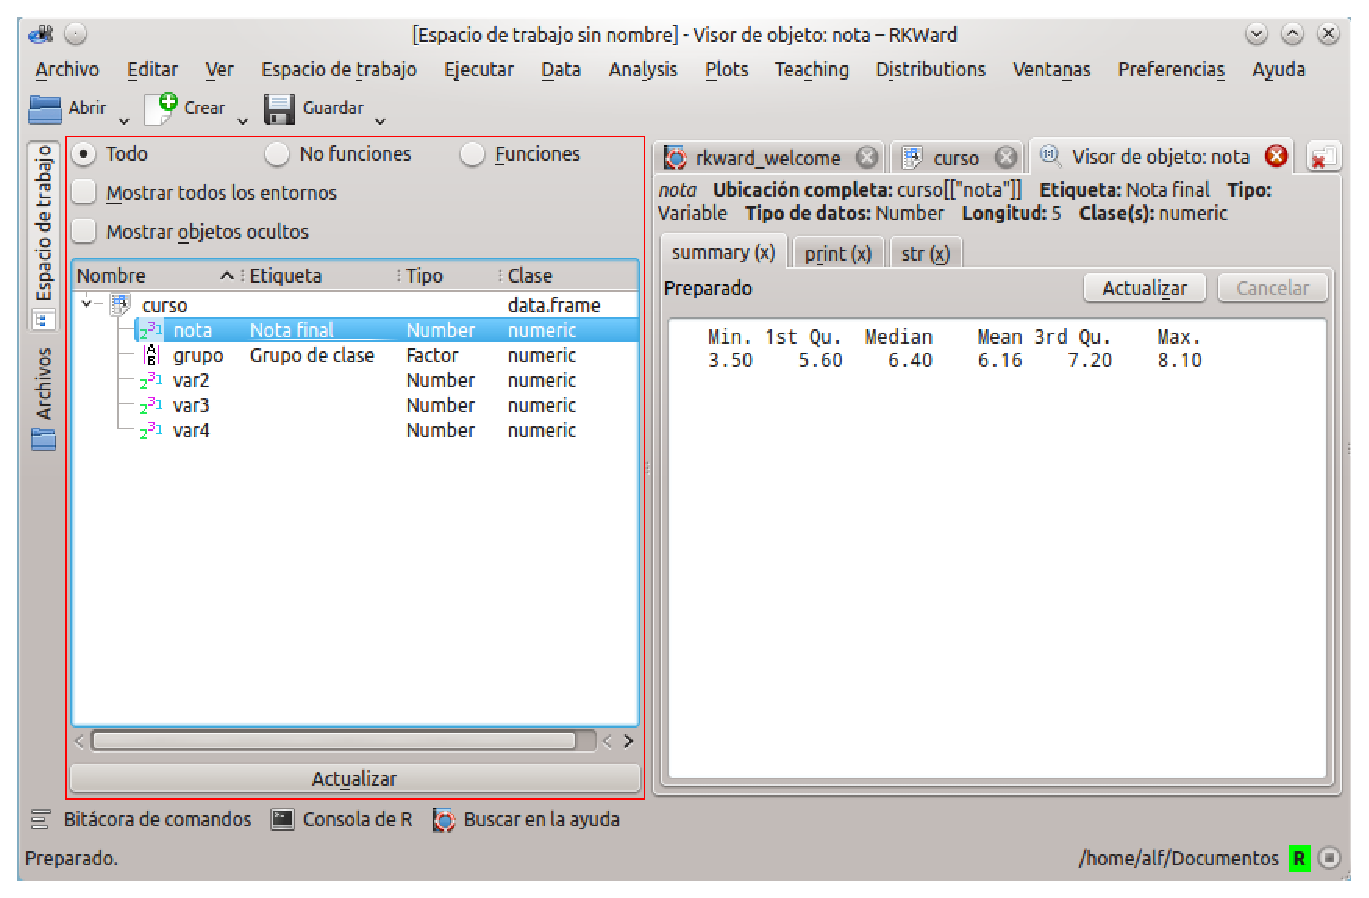
\includegraphics[scale=0.6]{introduccion_r/img/resumen_datos}
  \caption{Ventana de resumen descriptivo de un conjunto de datos}
  \label{g:resumen_datos}
\end{center}
\end{figure}

\subsection{Ponderación de datos}
Cuando una variable o un conjunto de datos tiene unos pocos valores que se repiten mucho, en lugar de teclearlos es más
rápido indicar los valores y ponderarlos por sus frecuencias.
Para ello se utiliza el menú \menu{Teaching>Datos>Ponerar datos}.
Al seleccionarlo aparece una ventana donde hay que seleccionar el conjunto de datos a ponderar, la variable numérica de
dicho conjunto de datos que contiene las frecuencias de ponderación, e indicar un nombre para el nuevo conjunto de datos.
Por ejemplo, si en una clase hay 20 chicas y 30 chicos, se puede crear un conjunto de datos con la variables sexo y
frequencia, tal y como se muestra en la figura~\ref{g:ponderar_variable1}, y después llamar al menú de ponderación con
los datos que aparencen la figura~\ref{g:ponderar_variable2}.

\begin{figure}[htp]
\begin{center}
  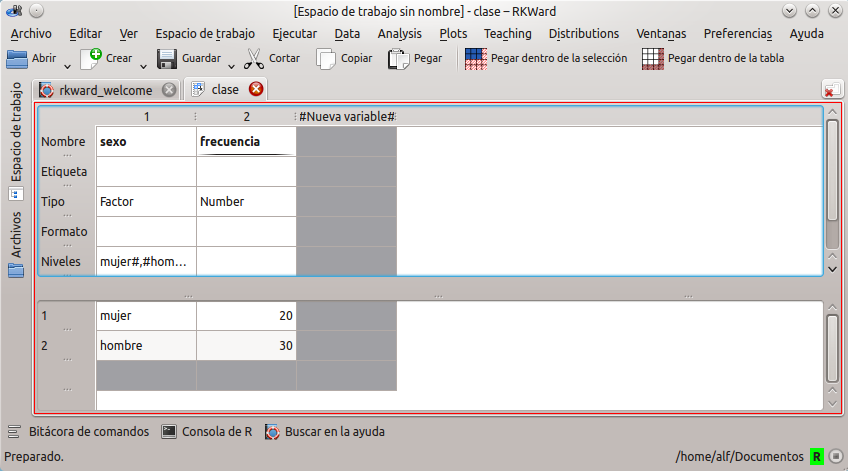
\includegraphics[scale=0.6]{introduccion_r/img/datos_frecuencias}
  \caption{Conjunto de datos preparado para ser ponderado}
  \label{g:ponderar_variable1}
\end{center}
\end{figure}

\begin{figure}[htp]
\begin{center}
  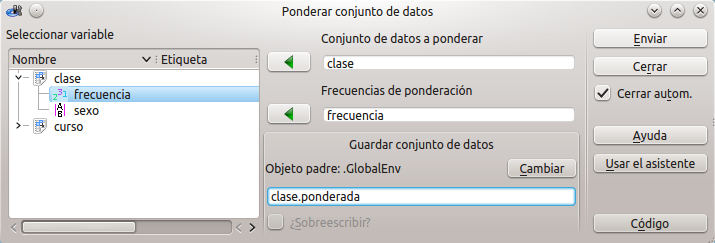
\includegraphics[scale=0.6]{introduccion_r/img/ponderacion}
  \caption{Ventana de ponderación de datos}
  \label{g:ponderar_variable2}
\end{center}
\end{figure}


\subsection{Guardar datos}
Una vez introducidos los datos, conviene guardarlos en un fichero para no tener que volver a introducirlos en futuras
sesiones. Para guardar los conjunto de datos definidos en el espacio de trabajo, se utiliza el menú \menu{Espacio de
trabajo>Guardar espacio de trabajo}.
Con esto aparece una ventana donde hay que darle un nombre al fichero y seleccionar la carpeta donde se guardará.
Los conjuntos de datos se guardan siempre en ficheros de R con extensión \comando{rda} o \comando{rData}.

También es posible guardar los datos en un fichero de texto plano mediante el menú \menu{Archivo>Exportar\flecha
Export tabular data}.
Tras esto aparece una ventana donde hay que seleccionar el conjunto de datos a exportar, darle un nombre al fichero de
texto y seleccionar la carpeta donde se guardará.
Esta ventana contiene también solapas donde se puede indicar entre otras cosas si incluir los nombres de las variables o
no, el separador de decimales o el separador de los datos, que puede ser un espacio, tabuladores, comas u otro caracter.


\subsection{Abrir datos}
Si los datos con los que se pretende trabajar ya están guardados en un fichero de R, entonces tendremos que abrir dicho
fichero. Para ello se utiliza el \menu{Espacio de trabajo>Abrir espacio de trabajo} y en la ventana que aparece
se selecciona el fichero que se desea abrir.
Automáticamente se cargará el conjunto de datos del fichero y pasará a ser el conjunto de datos activo.

También es posible cargar datos de ficheros con otros formatos, como por ejemplo un fichero de texto.
Para ello se utiliza el menú \menu{Archivo>Importar>Importar datos} y en la ventana que aparece se
selecciona el fichero de texto que se desea abrir y en el cuadro desplegable del formato de archivo se debes seleccionar
\opcion{Text}.
Después aparecerá una ventana donde habrá que darle un nombre al conjunto de datos y seleccionar el tipo de separador y
si los nombres de las variables aparecen en la primera línea del fichero.


\subsection{Eliminación de datos}
Para eliminar una variable del conjunto de datos primero hay que editar el conjunto de datos, y después, en la ventana
de edición de datos, hay que hacer clic con el botón derecho del ratón sobre la cabecera de la columna correspondiente
y seleccionar en el menú contextual que aparece \menu{Borrar esta variable}.

Para eliminar individuos del conjunto de datos que hacer clic con el botón derecho del ratón sobre la cabecera de la
fila correspondiente y seleccionar en el menú contextual que aparece \menu{Borrar esta fila}.

En la ventana del espacio de trabajo también es posible borrar cualquier objeto del espacio de trabajo de R haciendo
clic con el botón derecho del ratón sobre él y seleccionando el menú \menu{Eliminar}.


\section{Transformación de datos}
A menudo en los análisis hay que realizar transformaciones en los datos originales.
A continuación se presentan las transformaciones más habituales.


\subsection{Filtrado de datos}
Cuando se desea realizar un análisis con un subconjunto de individuos del conjunto de datos activo que cumplen una
determinada condición es posible filtrar el conjunto de datos para quedarse con esos individuos.
Para ello se utiliza el menú \menu{Teaching>Datos>Filtrar}.
Con esto aparece un cuadro de diálogo en el que hay que seleccionar el conjunto de datos que se desea filtrar, y en el
cuadro de texto \opcion{Condición de selección} indicar la condición lógica que tienen que cumplir los individuos
seleccionados.
También hay que indicar el nombre del nuevo conjunto de datos.
Por ejemplo, para seleccionar los alumnos del grupo de la mañana habría que indicar la condición
\lstinline{grupo==''m''} tal y como se muestra en la figura~\ref{g:filtrar_datos}.

\begin{figure}[htp]
\begin{center}
  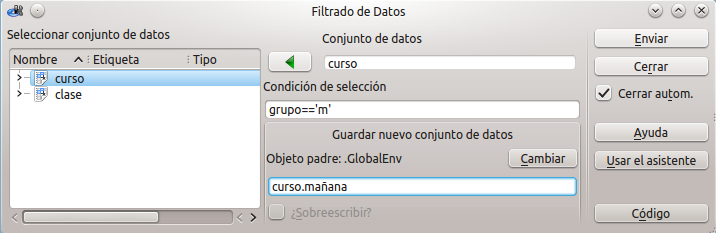
\includegraphics[scale=0.6]{introduccion_r/img/filtrar}
  \caption{Ventana de filtrado de datos.}
  \label{g:filtrar_datos}
\end{center}
\end{figure}


\subsection{Cálculo de variables}
Para calcular una nueva variable a partir de otras ya existentes en el espacio de trabajo de R se utiliza el menú
\menu{Teaching>Datos>Calcular variable}.
Con esto aparece un cuadro de diálogo en el que hay que introducir la expresión a partir de la que se calculará la nueva
variable en el cuadro de texto \opcion{Expresión de cálculo}, e indicar el nombre de la nueva variable.
La expresión de cálculo puede ser cualquier expresión aritmética o lógica de R, en las que pueden utilizarse cualquiera
de las variables del espacio de trabajo de R. Por ejemplo, para eliminar los decimales de la variable \variable{nota}
podría crearse una nueva variable \variable{puntuacion} multiplicando por 10 las notas, tal y como se muestra en la
figura~\ref{g:calcular_variable}.

\begin{figure}[htp]
\begin{center}
  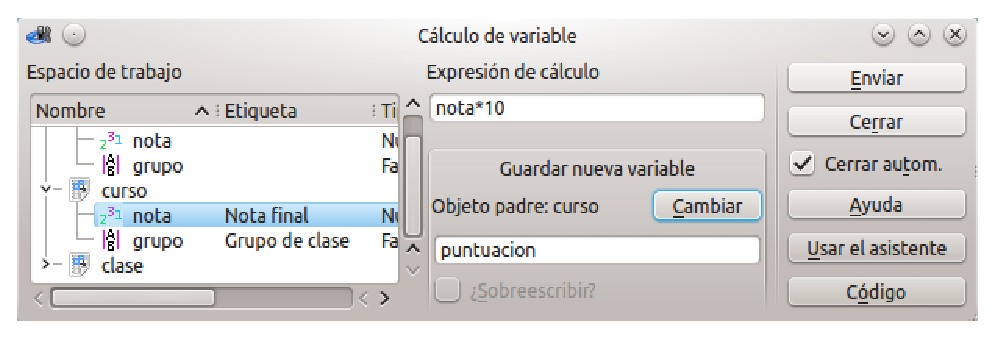
\includegraphics[scale=0.6]{introduccion_r/img/calcular}
  \caption{Ventana de cálculo de nuevas variables.}
  \label{g:calcular_variable}
\end{center}
\end{figure}


\subsection{Recodificación de variables}
Otra transformación habitual es la recodificación de variables que permite transformar los valores de una variable de
acuerdo a un conjunto de reglas de reescritura. Normalmente se utiliza para convertir una variable numérica en una
variable categórica que pueda usarse como un factor. 

Para recodificar una variable se utiliza el menú \menu{Teaching>Datos>Recodificar variable}.
Con esto aparece una ventana en la que hay que seleccionar la variable que se desea recodificar, indicar el nombre de la
nueva variable recodificada e introducir las reglas de recodificación en el cuadro de texto \opcion{Reglas de
recodificación}.
Las reglas de recodificación siempre siguen la sintaxis \lstinline{valor o rango de valores = nuevo valor} y pueden
introducirse tantas reglas como se desee, cada una en una línea.
Al lado izquierdo de la igualdad puede introducirse un único valor, varios valores separados por comas, o un rango de
valores indicando el límite inferior y el límite superior del intervalo separados por el operador \lstinline{:}.
A la hora de definir el límite inferior puede utilizarse la palabra clave \lstinline{lo} para referirse al menor de los
valores de la muestra y \lstinline{hi} para referirse al mayor de los valores.
Por ejemplo, para recodificar la variable \variable{nota} en categorías correspondientes a las calificaciones ([0-5)
Suspenso, [5,7) Aprobado, [7,9) Notable y [9,10] Sobresaliente), habría que introducir las reglas que se muestran en la
figura~\ref{g:recodificar_variable}. Después, en la ventana de introducción de datos, se pueden renombrar los niveles
del factor introduciendo el valor suspenso para la categoría 1, aprobado para la categoría 2, notable para la categoría
3 y sobresaliente para la categoría 4. 

\begin{figure}[htp]
\begin{center}
  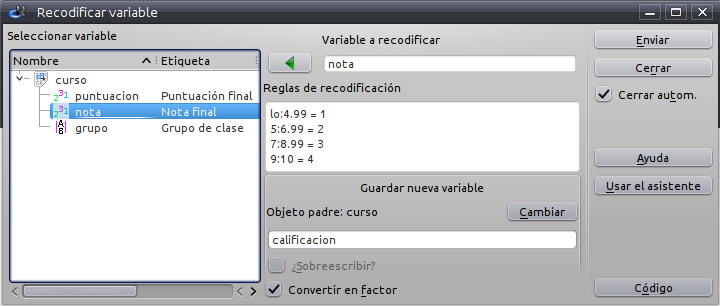
\includegraphics[scale=0.6]{introduccion_r/img/recodificar}
  \caption{Ventana de recodificación de variables}
  \label{g:recodificar_variable}
\end{center}
\end{figure} 


\section{Manipulación de ficheros de resultados}

\subsection{Guardar los resultados}
Cada vez que se ejecuta un comando de R, bien en la consola de comandos o a través de un menú, el comando ejecutado y su
salida quedan registrados en la bitácora de comandos. Sin embargo, esta salida es en texto plano sin formato por lo que
muchos de los procedimientos recogidos en los menús producen además una salida mucho más comprensible en formato HTML en
la ventana de resultados.

Para guardar el contenido de la ventana de resultados en un fichero se utiliza el menú \menu{Archivo>Exportar
página como HTML}.
Con esto aparece un cuadro de diálogo en el que hay que indicar el nombre del fichero y la carpeta donde se desea
guardar. El fichero resultante está en formato HTML por lo que se podrá visualizar con cualquier navegador web.

\subsection{Limpiar la ventana de resultados}
La vetana de resultados va acumulando todas las salidas de los análisis realizados en cada sesión de trabajo. 
Para no mezclar los resultados de estudios distintos, conviene limpiar la ventana de resultados cada vez que se empiece un estudio nuevo.
Para ello hay que seleccionar el menú \menu{Edición>Limpiar salida}.
 

\section{Manipulación de guiones de comandos}

\subsection{Creación de un guión de comandos}
RKWard también incorpora un entorno de desarrollo para programadores de R que permite crear guiones de comandos que
pueden ejecutarse todos seguidos.
Esta opción es muy interesante para repetir análisis o automatizar tareas repetitivas.
Para crear un guión de comandos hay que seleccionar el menú \menu{Archivo>Nuevo>Archivo de guiones}.
Con esto aparecerá una venta como la que aparece en la figura~\ref{g:guiones_comandos} donde se podrán teclecar los
comandos de R para después ejecutarlos uno a uno o en bloque.

\begin{figure}[htp]
\begin{center}
  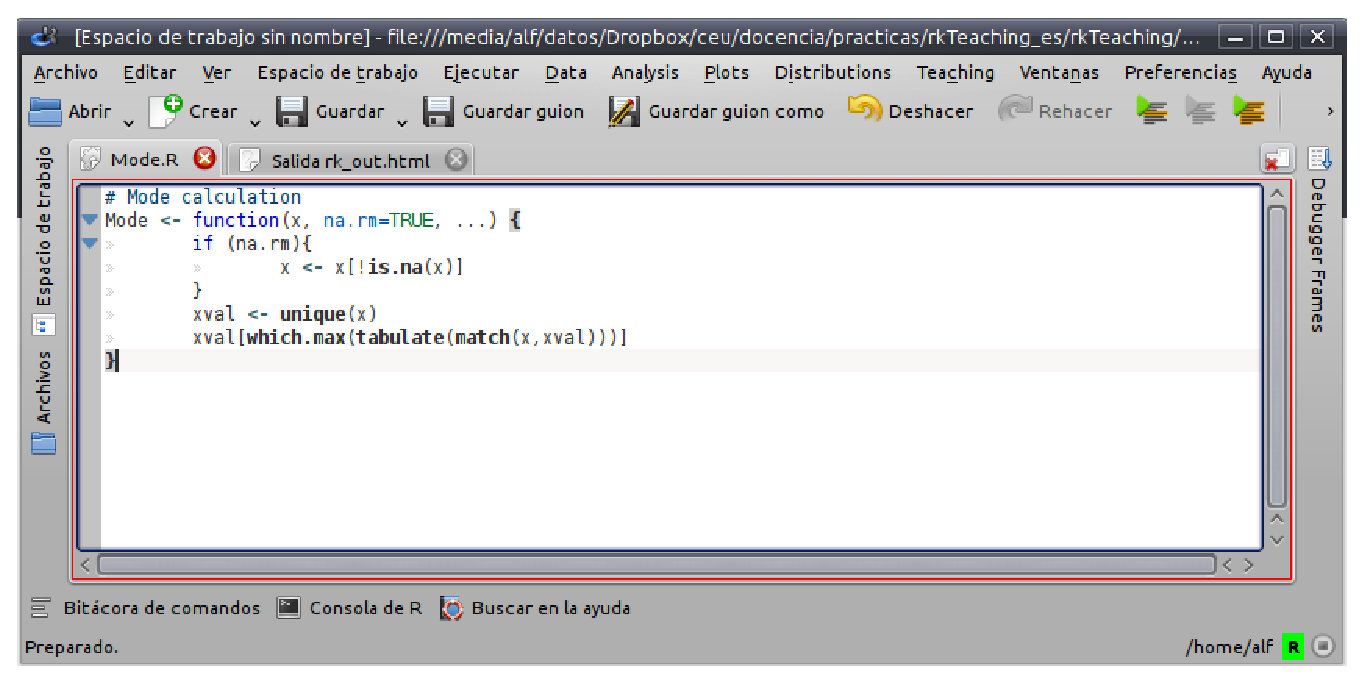
\includegraphics[scale=0.6]{introduccion_r/img/guiones_comandos}
  \caption{Ventana de edición de guiones de comandos}
  \label{g:guiones_comandos}
\end{center}
\end{figure}


\subsection{Guardar un guión de comandos}
Los guiones de comandos también pueden guardarse en un fichero de texto plano mediante el menú
\menu{Archivo>Guardar guión} e indicando el nombre del fichero y la carpeta donde se guardará en el
cuadro de diálo que aparece.


\subsection{Abrir un guión de comandos}
Para abrir un fichero con un guión de comandos se utiliza el menú \menu{Archivo>Abrir archivo de guiones de R} y
después seleccionar el fichero que se desea abrir en el cuadro de diálogo que aparece. 


\section{Ayuda}
Otra de las ventajas de R es que tiene un sistema de ayuda muy documentado. Es posible conseguir ayuda sobre cualquier
función, prodecimiento o paquete simplemente tecleando el comando \lstinline{help()}. Por ejemplo, para obtener ayuda
sobre el comando \lstinline{mean} se teclearía
\begin{lstlisting}
> help("mean")
\end{lstlisting}
y con esto aparecerá una ventana de ayuda donde se describe la función y también aparecen ejemplos que ilustran su uso. 
Si no se conoce exactamente el nombre de la función o comando, se puede hacer una búsqueda aproximada con el comando
\lstinline{help.search()}. Por emplo, si no se recuerda el nombre de la función logarítmica, se podría
teclear
\begin{lstlisting}
> help("logarithm")
\end{lstlisting}
y con esto aparecerá una ventana con todos los ficheros de ayuda que contienen la palabra logarithm.

Finalmente, también es posible invocar la ayuda general de R en RKWard con el menú \menu{Ayuda>Ayuda de R} con lo
que aparecerá una página web desde donde podremos navegar a la información deseada. También es posible buscar ayuda
sobre un comando concreto en el menú \menu{Ayuda>Buscar en la ayuda de R}.

Para más información sobre R se recomienda visitar la página \url{http://www.r-project.org/}, y para más información
sobre RKWard se recomienda visitar la página \url{http://rkward.sourceforge.net/}. 

\clearpage
\newpage

\section{Ejercicios resueltos}
\begin{enumerate}[leftmargin=*]
\item Crear un conjunto de datos con los datos de la siguiente muestra y guardarlo con el nombre
\comando{colesterol.rda}
\begin{center}
\begin{tabular}{|l|c|r|r|r|}
\hline
\multicolumn{1}{|c|}{Nombre} & \multicolumn{1}{c|}{Sexo} & \multicolumn{1}{c|}{Peso} & \multicolumn{1}{c|}{Altura} & \multicolumn{1}{c|}{Colesterol}\\
\hline
José Luis Martínez Izquierdo  & H &  85 & 179 & 182\\
Rosa Díaz Díaz & M & 65 & 173 & 232\\
Javier García Sánchez  & H & 71 & 181 & 191\\
Carmen López Pinzón & M &  65 & 170 & 200\\
Marisa López Collado & M &  51 & 158 & 148\\
Antonio Ruiz Cruz & H & 66 & 174 & 249\\
\hline
\end{tabular}
\end{center}

\begin{indicacion}
Para crear el conjunto de datos:
\begin{enumerate}
\item Seleccionar el menú \menu{Archivo>Nuevo>Conjunto de datos}.
\item En el cuadro de diálogo que aparece introducir el nombre del conjunto de datos \variable{colesterol} y hacer clic en el botón \boton{Aceptar}.
\item En la ventana del editor de datos hay que definir una variable en cada columna introduciendo su nombre y tipo en las casillas de la cabecera de cada columna.
\item Una vez definidas las variables hay que introducir los datos de cada variable en la columna correspondiente. 
\end{enumerate}
Para guardar los datos:
\begin{enumerate}
\item Selecionar el menú \menu{Espacio de trabajo>Guardar espacio de trabajo}.
\item En el cuadro de diálogo que aparece hay que darle un nombre al fichero, seleccionar la carpeta donde guardarlo y hacer clic en el
botón \boton{Aceptar}.
\end{enumerate}
\end{indicacion}

\item Abrir el fichero creado en el ejercicio anterior y realizar las siguientes operaciones:

\begin{enumerate}
\item Insertar una nueva variable \variable{Edad} con las edades de todos los individuos de la muestra.
\begin{center}
\begin{tabular}{|l|r|}
\hline
\multicolumn{1}{|c|}{Nombre} & \multicolumn{1}{c|}{Edad} \\
\hline
José Luis Martínez Izquierdo & 18 \\
Rosa Díaz Díaz & 32 \\
Javier García Sánchez & 24 \\
Carmen López Pinzón & 35 \\
Marisa López Collado & 46 \\
Antonio Ruiz Cruz & 68 \\
\hline
\end{tabular}
\end{center}

\begin{indicacion} 
Para abrir el conjunto de datos del ejercicio anterior:
\begin{enumerate}
\item Seleccionar el menú \menu{Espacio de trabajo>Abrir espacio de trabajo}.
\item En el cuadro de diálogo que aparece seleccionar la carpeta donde se encuentra el fichero con los datos del ejercicio anterior,
seleccionar el fichero y hacer clic en el botón \boton{Aceptar}.
\end{enumerate}
Para insertar la variable \variable{Edad}:
\begin{enumerate}
\item Hacer clic en la solapa \boton{Espacio de trabajo}.
\item En la ventana del espacio de trabajo doble clic sobre el conjunto de datos \variable{colesterol}.
\item En la ventana del editor de datos introducir el nombre de la variable \variable{edad} y su tipo en las casillas de la cabecera de una nueva columna vacía, e introducir los datos de las edades en las celdas de maś abajo. 
\end{enumerate}
\end{indicacion}

\item Insertar un nuevo individuo con siguientes datos
\begin{quote}
Nombre: Cristóbal Campos Ruiz.\\
Edad: 44 años.\\
Sexo: Hombre.\\
Peso: 70 Kg.\\
Altura: 178 cm.\\
Colesterol: 220 mg/dl.
\end{quote}

\begin{indicacion}
\begin{enumerate}
\item En la ventana del editor de datos introducir los datos de del nuevo individuo en la primera fila vacía.
\end{enumerate}
\end{indicacion}

\item Crear una nueva variable donde se calcule el índice de masa corporal de cada paciente mediante la formula:
\[
\text{imc} = \frac{\text{Peso (en Kg)}}{\text{Altura (en mt)}^2}
\]

\begin{indicacion}
\begin{enumerate}
\item Seleccionar el menú \menu{Teaching>Datos>Calcular variable}.
\item En el cuadro de diálogo que aparece introducir la fórmula para calcular el índice de masa
corporal en el campo \campo{Expresión de cálculo}.
\item En el cuadro \campo{Guardar nueva variable} hacer clic sobre el botón \boton{Cambiar}.
\item En el cuadro de diálogo que aparece seleccionar como objeto padre la el conjunto de datos \variable{colesterol} y hacer clic sobre el botón \boton{Aceptar}.
\item Introducir el nombre de la nueva variable \variable{imc} y hacer clic sobre el botón \boton{Aceptar}.
\end{enumerate}
\end{indicacion}

\item Recodificar el índice de masa corporal en una nueva variable de acuerdo a las siguientes categorías:
\begin{center}
\begin{tabular}{ll}
Menor de $18.5$ & Bajo peso\\
De $18.5$ a $24.5$ & Saludable\\
De $24.5$ a $30$ & Sobrepeso\\
Mayor de $30$  & Obeso
\end{tabular}
\end{center}

\begin{indicacion}
\begin{enumerate}
\item Selecionar el menú \menu{Teaching>Datos>Recodificar variable}.
\item En el cuadro de diálogo que aparece seleccionar como variable a recodificar la variable \variable{imc}.
\item Introducir las reglas de recodificación en el campo \campo{Reglas de recodificación}:
\begin{quote}
\lstinline{lo:18.5 = 1}\\
\lstinline{18.5:24.5 = 2}\\
\lstinline{24.5:30 = 3}\\
\lstinline{30:hi = 4}
\end{quote}
\item En el cuadro \campo{Guardar nueva variable} hacer clic sobre el botón \boton{Cambiar}.
\item En el cuadro de diálogo que aparece seleccionar como objeto padre la el conjunto de datos \variable{colesterol} y hacer clic sobre el botón \boton{Aceptar}.
\item Introducir el nombre de la nueva variable \variable{obesidad} y hacer clic sobre el botón \boton{Aceptar}.
\item En la ventada de edición de datos introducir los niveles del factor, asignando Bajo peso a la categoría 1,
Saludable a la categoría 2, Sobrepeso a la categoría 3 y Obeso a la categoría 4. 
\end{enumerate}
\end{indicacion}


\item Filtrar el conjunto de datos para obtener un nuevo conjunto de datos con los datos de los hombres
\begin{indicacion}
\begin{enumerate}
\item Selecionar el menú \menu{Teaching>Datos>Filtrar}.
\item En el cuadro de diálogo que aparece seleccionar como conjunto de datos \variable{colesterol}.
\item En el campo \campo{Condición de selección} introducir la condición \lstinline{sexo=="H"}. 
\item Introducir el nombre del  nuevo conjunto de datos \variable{colesterol.hombres} y hacer clic sobre el botón \boton{Aceptar}.
\end{enumerate}
\end{indicacion}
%\item Importar el conjunto de datos del fichero de texto \comando{Nations.txt} que se encuentra en el subdirectorio \comando{etc} del
% paquete \comando{Rcmdr} y visualizar el conjunto de datos.

%\item Filtrar el conjunto de datos para quedarse únicamente con los países de Europa.

\end{enumerate}
\end{enumerate}

\section{Ejercicios propuestos}
\begin{enumerate}[leftmargin=*]
\item  El conjunto de datos \variable{neonatos} del paquete \variable{rk.Teaching}, contiene información sobre una
muestra de 320 recién nacidos en un hospital durante un año que cumplieron el tiempo normal de gestación. 
Se pide:
\begin{enumerate}
\item Cargar el conjunto de datos.
\begin{indicacion}
\begin{enumerate}
\item Hacer clic en la solapa \campo{Espacio de trabajo} para desplegarla y ver los paquetes del espacio de trabajo. 
\item Hacer doble clic sobre el paquete \variable{rk.Teaching} para ver todos los conjuntos de datos que contiene. 
\item Hacer clic con el botón derecho sobre el conjunto de datos \variable{nenonatos} y en el menú contextual que
aparece selecconar \menu{Copiar a .GlobalEnv} para hacer una copia del conjunto de datos en nuestro entorno de trabajo. 
\end{enumerate}
\end{indicacion}

\item Calcular la variable \variable{apgar.medio} como la media de las variables \variable{apgar1} y \variable{apgar5}.
\item Recodificar la varible \variable{peso} en el factor \variable{categoria.peso} con dos categorias que se
correspondan con los pesos menores y mayores de $2.5$ Kg.
\item Recodificar la variable \variable{apgar1} en el factor \variable{estado.apgar1} con tres categorías: deprimido
(Apgar$\leq 3$), moderadamente deprimido ($3<$Apgar$\leq 6$) y normal (Apgar$>6$).
\item Filtrar el conjunto de datos para quedarse con los hijos de las madres no fumadoras con una puntuación Apgar al
minuto de nacer menor o igual que 3. ¿Cuántos niños hay?
\end{enumerate}
\end{enumerate}
\chapter[Distribuciones de Frecuencias y Representaciones Gráficas]{Distribuciones de Frecuencias\\ y Representaciones Gráficas}

\section{Fundamentos teóricos}
Uno de los primeros pasos en cualquier estudio estadístico es el resumen y la descripción de la información contenida en
una muestra. Para ello se van a aplicar algunos métodos de análisis descriptivo, que nos permitirán clasificar y
estructurar la información al igual que representarla gráficamente.

Las características que estudiamos pueden ser o no susceptibles de medida; en este sentido definiremos una
\emph{variable} como un carácter susceptible de ser medido, es decir, cuantitativo y cuantificable mediante la
observación, (por ejemplo el peso de las personas, la edad, etc...), y definiremos un \emph{atributo} como un carácter
no susceptible de ser medido, y en consecuencia observable tan sólo cualitativamente (por ejemplo el color de ojos,
estado de un paciente, etc...). Se llaman modalidades a las posibles observaciones de un atributo.

Dentro de los atributos, podemos hablar de \emph{atributos ordinales}, los que presentan algún tipo de orden entre las
distintas modalidades, y de \emph{atributos nominales}, en los que no existe ningún orden entre ellas.

Dentro de las variables podemos diferenciar entre \emph{discretas}, si sus valores posibles son valores aislados, y
\emph{continuas}, si pueden tomar cualquier valor dentro de un intervalo.

En algunos textos no se emplea el término \emph{atributo} y se denominan a todos los caracteres \emph{variables}. En ese
caso se distinguen \emph{variables cuantitativas} para designar las que aquí hemos definido como \emph{variables}, y
\emph{variables cualitativas} para las que aquí se han llamado \emph{atributos}. En lo sucesivo se aplicará este
criterio para simplificar la exposición.


\subsection{Cálculo de Frecuencias}
Para estudiar cualquier característica, lo primero que deberemos hacer es un recuento de las observaciones, y el número
de repeticiones de éstas. Para cada valor $x_i$ de la muestra se define:
\begin{description}
\item[Frecuencia absoluta] Es el número de veces que aparece cada uno de los valores $x_i$ y se denota por $n_i$.

\item [Frecuencia relativa] Es el número de veces que aparece cada valor $x_i$ dividido entre el tamaño muestral y se
denota por $f_i$

\[f_i=\frac{n_i}{n}\]

Generalmente las frecuencias relativas se multiplican por $100$ para que representen el tanto por ciento.
\end{description}

En el caso de que exista un orden entre los valores de la variable, a veces nos interesa no sólo conocer el número de
veces que se repite un determinado valor, sino también el número de veces que aparece dicho valor y todos los menores. A
este tipo de frecuencias se le denomina \emph{frecuencias acumuladas}.

\begin{description}
\item [Frecuencia absoluta acumulada] Es la suma de las frecuencias absolutas de los valores menores que $x_i$ más la frecuencia
absoluta de $x_i$, y se denota por $N_i$

\[N_i=n_1+n_2+\ldots+n_i\]

\item [Frecuencia relativa acumulada] Es la suma de las frecuencias relativas de los valores menores que $x_i$ más la frecuencia
relativa de $x_i$, y se denota por $F_i$

\[F_i=f_1+f_2+\ldots+f_i\]
\end{description}

Los resultados de las observaciones de los valores de una variable estadística en una muestra suelen representarse en
forma de tabla.
En la primera columna se representan los valores $x_i$ de la variable colocados en orden creciente, y en la siguiente
columna los valores de las frecuencias absolutas correspondientes $n_i$.

Podemos completar la tabla con otras columnas, correspondientes a las frecuencias relativas, $f_i$, y a las frecuencias
acumuladas, $N_i$ y $F_i$. Al conjunto de los valores de la variable observados en la muestra junto con sus frecuencias
se le conoce como \emph{distribución de frecuencias muestral}.

\begin{ejemplo}
En una encuesta a 25 matrimonios, sobre el número de hijos que tienen, se obtienen los siguientes datos:
\begin{center}
1, 2, 4, 2, 2, 2, 3, 2, 1, 1, 0, 2, 2, 0, 2, 2, 1, 2, 2, 3, 1, 2,
2, 1, 2.
\end{center}

Los valores distintos de la variable son: 0, 1, 2, 3 y 4. Así la tabla será:
  \[\begin{array}{|c|l|r|}
    \hline
    x_i & \mbox{Recuento} & n_i \\ \hline
    0 & \mbox{II} & 2 \\
    1 & \mbox{IIIII I} & 6 \\
    2 & \mbox{IIIII IIIII IIII} & 14 \\
    3 & \mbox{II} & 2 \\
    4 & \mbox{I} & 1 \\ \hline

  \end{array}
  \]

La distribución de las frecuencias quedaría:
  \[\begin{array}{|c|c|c|c|c|}
    \hline
    x_i & n_i & f_i & N_i & F_i \\ \hline
    0 & 2 & 0.08 & 2 & 0.08 \\ \hline
    1 & 6 & 0.24 & 8 & 0.32 \\ \hline
    2 & 14 & 0.56 & 22 & 0.88 \\ \hline
    3 & 2 & 0.08 & 24 & 0.96 \\ \hline
    4 & 1 & 0.04 & 25 & 1 \\ \hline
    \mbox{Suma} & 25 & 1 & \multicolumn{2}{c}{} \\
    \cline{1-3}
  \end{array}
  \]
\end{ejemplo}

Cuando el tamaño de la muestra es grande en el caso de variables discretas con muchos valores distintos de la variable,
y en cualquier caso si se trata de variables continuas, se agrupan las observaciones en \emph{clases}, que son
intervalos contiguos, preferiblemente de la misma amplitud.

Para decidir el número de clases a considerar, una regla frecuentemente utilizada es tomar el entero más próximo a
$\sqrt{n}$ donde $n$ es el número de observaciones en la muestra. Pero conviene probar con distintos números de clases y
escoger el que proporcione una descripción más clara. Así se prefijan los intervalos $(a_{i-1},a_i] , i=1,2,\ldots,l$
siendo $a=a_0<a_1<....<a_l=b$ de tal modo que todos los valores observados estén dentro del intervalo $(a, b]$, y sin
que exista ambig\"{u}edad a la hora de decidir a qué intervalo pertenece cada dato.

Llamaremos \emph{marca de clase} al punto medio de cada intervalo.
Así la \emph{marca de la clase} $(a_{i-1},a_i]$ es el punto medio $x_i$ de dicha clase, es decir

\[  x_i=\frac{a_{i-1}+a_i}{2} \]

En el tratamiento estadístico de los datos agrupados, todos los valores que están en una misma clase se consideran
iguales a la marca de la clase. De esta manera si en la clase $(a_{i-1},a_i]$ hay $n_i$ valores observados, se puede
asociar la marca de la clase $x_i$ con esta frecuencia $n_i$.



\subsection{Representaciones Gráficas}
Hemos visto que la tabla estadística resume los datos de una muestra, de forma que ésta se puede analizar de una manera
más sistemática y resumida. Para conseguir una percepción visual de las carac\-terísticas de la población resulta muy
útil el uso de gráficas y diagramas. Dependiendo del tipo de variable y de si trabajamos con datos agrupados o no, se
utilizarán distintos tipos.


\subsubsection{Diagrama de barras y polígono de frecuencias}
Consiste en representar sobre el eje de abscisas de un sistema de ejes coordenados los distintos valores de la variable
$X$, y levantar sobre cada uno de esos puntos una barra cuya altura sea igual a la frecuencia absoluta o relativa
correspondiente a ese valor, tal y como se muestra en la figura \ref{g:diagramaabsolutas}.
Esta representación se utiliza para distribuciones de frecuencias con pocos valores distintos de la variable, tanto
cuantitativas como cualitativas, y en este último caso se suele representar con rectángulos de altura igual a la
frecuencia de cada modalidad.

En el caso de variables cuantitativas se puede representar también el diagrama de barras de las frecuencias acumuladas,
tal y como se muestra en la figura \ref{g:diagramaacumuladas}.

Otra representación habitual es el \emph{polígono de frecuencias} que consiste en la línea poligonal cuyos vertices son
los puntos $(x_i,n_i)$, tal y como se ve en la figura \ref{g:poligonoabsolutas}, y si en vez de considerar las
frecuencias absolutas o relativas se consideran las absolutas o relativas acumuladas, se obtiene el \emph{polígono de
frecuencias acumuladas}, como se ve en la figura \ref{g:poligonoacumuladas}.

\begin{figure}[h!]
\centering
\subfigure[Diagrama de barras de frecuencias absolutas.]{\label{g:diagramaabsolutas}
\scalebox{0.65}{%% Input file name: diagrama_barras_frecuencia_absoluta.fig
%% FIG version: 3.2
%% Orientation: Landscape
%% Justification: Flush Left
%% Units: Inches
%% Paper size: A4
%% Magnification: 100.0
%% Resolution: 1200ppi

\begin{pspicture}(6.70cm,3.48cm)(16.66cm,13.45cm)
\psset{unit=0.8cm}
%%
%% Depth: 2147483647
%%
\newgray{mycolor0}{0.74}\definecolor{mycolor0}{gray}{0.74}
\newrgbcolor{mycolor1}{1.00 0.50 0.31}\definecolor{mycolor1}{rgb}{1.00,0.50,0.31}
%%
%% Depth: 100
%%
\psset{linestyle=solid,linewidth=0.03175,linecolor=black,fillstyle=solid,fillcolor=mycolor0}
\pspolygon(10.92,6.47)(10.92,6.47)(12.47,6.47)(12.47,6.47)(10.92,6.47)
\psset{fillstyle=none}
\psline(10.23,6.47)(10.23,15.28)
\psline(10.23,6.47)(10.02,6.47)
\psline(10.23,7.73)(10.02,7.73)
\psline(10.23,8.99)(10.02,8.99)
\psline(10.23,10.25)(10.02,10.25)
\psline(10.23,11.50)(10.02,11.50)
\psline(10.23,12.76)(10.02,12.76)
\psline(10.23,14.02)(10.02,14.02)
\psline(10.23,15.28)(10.02,15.28)
\rput{90}(9.73,6.47){0}
\rput{90}(9.73,7.73){2}
\rput{90}(9.73,8.99){4}
\rput{90}(9.73,10.25){6}
\rput{90}(9.73,11.50){8}
\rput{90}(9.73,12.76){10}
\rput{90}(9.73,14.02){12}
\rput{90}(9.73,15.28){14}
\psset{linestyle=dotted,linecolor=mycolor0}
\psline(10.23,6.47)(20.31,6.47)
\psline(10.23,7.73)(20.31,7.73)
\psline(10.23,8.99)(20.31,8.99)
\psline(10.23,10.25)(20.31,10.25)
\psline(10.23,11.50)(20.31,11.50)
\psline(10.23,12.76)(20.31,12.76)
\psline(10.23,14.02)(20.31,14.02)
\psset{linestyle=solid,linecolor=black,fillstyle=solid,fillcolor=mycolor1}
\pspolygon(10.92,6.47)(10.92,7.73)(12.47,7.73)(12.47,6.47)(10.92,6.47)
\pspolygon(12.78,6.47)(12.78,10.25)(14.34,10.25)(14.34,6.47)(12.78,6.47)
\pspolygon(14.65,6.47)(14.65,15.28)(16.21,15.28)(16.21,6.47)(14.65,6.47)
\pspolygon(16.52,6.47)(16.52,7.73)(18.07,7.73)(18.07,6.47)(16.52,6.47)
\pspolygon(18.38,6.47)(18.38,7.10)(19.94,7.10)(19.94,6.47)(18.38,6.47)
\rput(11.70,5.71){0}
\rput(13.56,5.71){1}
\rput(15.43,5.71){2}
\rput(17.29,5.71){3}
\rput(19.16,5.71){4}
%\rput(15.27,15.99){\Large Diagrama de barras de frecuencias absolutas}
\rput(15.27,4.86){\large Número de hijos}
\rput[l]{90}(8.89,8.75){\large Frecuencia absoluta $n_i$}
\psset{fillstyle=none}
\psline(10.23,6.47)(10.23,15.28)
\psline(10.23,6.47)(10.02,6.47)
\psline(10.23,7.73)(10.02,7.73)
\psline(10.23,8.99)(10.02,8.99)
\psline(10.23,10.25)(10.02,10.25)
\psline(10.23,11.50)(10.02,11.50)
\psline(10.23,12.76)(10.02,12.76)
\psline(10.23,14.02)(10.02,14.02)
\psline(10.23,15.28)(10.02,15.28)
\rput{90}(9.73,6.47){0}
\rput{90}(9.73,7.73){2}
\rput{90}(9.73,8.99){4}
\rput{90}(9.73,10.25){6}
\rput{90}(9.73,11.50){8}
\rput{90}(9.73,12.76){10}
\rput{90}(9.73,14.02){12}
\rput{90}(9.73,15.28){14}
\end{pspicture}
%% End
}}\qquad
\subfigure[Diagrama de barras de frecuencias absolutas acumuladas.]{\label{g:diagramaacumuladas}
\scalebox{0.65}{%% Input file name: diagrama_barras_frecuencia_acumulada.fig
%% FIG version: 3.2
%% Orientation: Landscape
%% Justification: Flush Left
%% Units: Inches
%% Paper size: A4
%% Magnification: 100.0
%% Resolution: 1200ppi

\begin{pspicture}(6.70cm,3.48cm)(17.30cm,13.45cm)
\psset{unit=0.8cm}
%%
%% Depth: 2147483647
%%
\newgray{mycolor0}{0.74}\definecolor{mycolor0}{gray}{0.74}
\newrgbcolor{mycolor1}{1.00 0.50 0.31}\definecolor{mycolor1}{rgb}{1.00,0.50,0.31}
%%
%% Depth: 100
%%
\psset{linestyle=solid,linewidth=0.03175,linecolor=black,fillstyle=solid,fillcolor=mycolor0}
\pspolygon(10.61,6.56)(10.61,7.26)(12.22,7.26)(12.22,6.56)(10.61,6.56)
\pspolygon(12.54,6.56)(12.54,9.35)(14.15,9.35)(14.15,6.56)(12.54,6.56)
\pspolygon(14.47,6.56)(14.47,14.23)(16.08,14.23)(16.08,6.56)(14.47,6.56)
\pspolygon(16.40,6.56)(16.40,14.93)(18.01,14.93)(18.01,6.56)(16.40,6.56)
\pspolygon(18.33,6.56)(18.33,15.28)(19.94,15.28)(19.94,6.56)(18.33,6.56)
\psset{fillstyle=none}
\psline(10.23,6.56)(10.23,15.28)
\psline(10.23,6.56)(10.02,6.56)
\psline(10.23,8.30)(10.02,8.30)
\psline(10.23,10.05)(10.02,10.05)
\psline(10.23,11.79)(10.02,11.79)
\psline(10.23,13.53)(10.02,13.53)
\psline(10.23,15.28)(10.02,15.28)
\rput{90}(9.73,6.56){0}
\rput{90}(9.73,8.30){5}
\rput{90}(9.73,10.05){10}
\rput{90}(9.73,11.79){15}
\rput{90}(9.73,13.53){20}
\rput{90}(9.73,15.28){25}
\psset{linestyle=dotted,linecolor=mycolor0}
\psline(10.23,6.56)(20.31,6.56)
\psline(10.23,7.26)(20.31,7.26)
\psline(10.23,7.95)(20.31,7.95)
\psline(10.23,8.65)(20.31,8.65)
\psline(10.23,9.35)(20.31,9.35)
\psline(10.23,10.05)(20.31,10.05)
\psline(10.23,10.74)(20.31,10.74)
\psline(10.23,11.44)(20.31,11.44)
\psline(10.23,12.14)(20.31,12.14)
\psline(10.23,12.84)(20.31,12.84)
\psline(10.23,13.53)(20.31,13.53)
\psline(10.23,14.23)(20.31,14.23)
\psline(10.23,14.93)(20.31,14.93)
\psset{linestyle=solid,linecolor=black,fillstyle=solid,fillcolor=mycolor1}
\pspolygon(10.61,6.56)(10.61,7.26)(12.22,7.26)(12.22,6.56)(10.61,6.56)
\pspolygon(12.54,6.56)(12.54,9.35)(14.15,9.35)(14.15,6.56)(12.54,6.56)
\pspolygon(14.47,6.56)(14.47,14.23)(16.08,14.23)(16.08,6.56)(14.47,6.56)
\pspolygon(16.40,6.56)(16.40,14.93)(18.01,14.93)(18.01,6.56)(16.40,6.56)
\pspolygon(18.33,6.56)(18.33,15.28)(19.94,15.28)(19.94,6.56)(18.33,6.56)
\rput(11.41,5.71){0}
\rput(13.34,5.71){1}
\rput(15.27,5.71){2}
\rput(17.20,5.71){3}
\rput(19.13,5.71){4}
%\rput(15.27,15.99){Diagrama de barras de frecuencias absolutas acumuladas}
\rput(15.27,4.86){Número de hijos}
\rput[l]{90}(8.89,7.61){Frecuencia absoluta acumulada $N_i$}
\psset{fillstyle=none}
\psline(10.23,6.56)(10.23,15.28)
\psline(10.23,6.56)(10.02,6.56)
\psline(10.23,8.30)(10.02,8.30)
\psline(10.23,10.05)(10.02,10.05)
\psline(10.23,11.79)(10.02,11.79)
\psline(10.23,13.53)(10.02,13.53)
\psline(10.23,15.28)(10.02,15.28)
\rput{90}(9.73,6.56){0}
\rput{90}(9.73,8.30){5}
\rput{90}(9.73,10.05){10}
\rput{90}(9.73,11.79){15}
\rput{90}(9.73,13.53){20}
\rput{90}(9.73,15.28){25}
\end{pspicture}
%% End
}}\\
\subfigure[Polígono de frecuencias absolutas.]{\label{g:poligonoabsolutas}
\scalebox{0.65}{%% Input file name: diagrama_barras_frecuencia_absoluta.fig
%% FIG version: 3.2
%% Orientation: Landscape
%% Justification: Flush Left
%% Units: Inches
%% Paper size: A4
%% Magnification: 100.0
%% Resolution: 1200ppi

\begin{pspicture}(6.70cm,3.48cm)(16.66cm,13.45cm)
\psset{unit=0.8cm}
%%
%% Depth: 2147483647
%%
\newgray{mycolor0}{0.74}\definecolor{mycolor0}{gray}{0.74}
\newrgbcolor{mycolor1}{1.00 0.50 0.31}\definecolor{mycolor1}{rgb}{1.00,0.50,0.31}
\newrgbcolor{mycolor2}{0.25 0.41 0.88}\definecolor{mycolor2}{rgb}{0.25,0.41,0.88}
%%
%% Depth: 100
%%
\psset{linestyle=solid,linewidth=0.03175,linecolor=black,fillstyle=solid,fillcolor=mycolor0}
\pspolygon(10.92,6.47)(10.92,6.47)(12.47,6.47)(12.47,6.47)(10.92,6.47)
\psset{fillstyle=none}
\psline(10.23,6.47)(10.23,15.28)
\psline(10.23,6.47)(10.02,6.47)
\psline(10.23,7.73)(10.02,7.73)
\psline(10.23,8.99)(10.02,8.99)
\psline(10.23,10.25)(10.02,10.25)
\psline(10.23,11.50)(10.02,11.50)
\psline(10.23,12.76)(10.02,12.76)
\psline(10.23,14.02)(10.02,14.02)
\psline(10.23,15.28)(10.02,15.28)
\rput{90}(9.73,6.47){0}
\rput{90}(9.73,7.73){2}
\rput{90}(9.73,8.99){4}
\rput{90}(9.73,10.25){6}
\rput{90}(9.73,11.50){8}
\rput{90}(9.73,12.76){10}
\rput{90}(9.73,14.02){12}
\rput{90}(9.73,15.28){14}
\psset{linestyle=dotted,linecolor=mycolor0}
\psline(10.23,6.47)(20.31,6.47)
\psline(10.23,7.73)(20.31,7.73)
\psline(10.23,8.99)(20.31,8.99)
\psline(10.23,10.25)(20.31,10.25)
\psline(10.23,11.50)(20.31,11.50)
\psline(10.23,12.76)(20.31,12.76)
\psline(10.23,14.02)(20.31,14.02)
\psset{linestyle=solid,linecolor=black,fillstyle=solid,fillcolor=mycolor1}
\pspolygon(10.92,6.47)(10.92,7.73)(12.47,7.73)(12.47,6.47)(10.92,6.47)
\pspolygon(12.78,6.47)(12.78,10.25)(14.34,10.25)(14.34,6.47)(12.78,6.47)
\pspolygon(14.65,6.47)(14.65,15.28)(16.21,15.28)(16.21,6.47)(14.65,6.47)
\pspolygon(16.52,6.47)(16.52,7.73)(18.07,7.73)(18.07,6.47)(16.52,6.47)
\pspolygon(18.38,6.47)(18.38,7.10)(19.94,7.10)(19.94,6.47)(18.38,6.47)
\rput(11.70,5.71){0}
\rput(13.56,5.71){1}
\rput(15.43,5.71){2}
\rput(17.29,5.71){3}
\rput(19.16,5.71){4}
%\rput(15.27,15.99){\Large Diagrama de barras de frecuencias absolutas}
\rput(15.27,4.86){Número de hijos}
\rput[l]{90}(8.89,8.75){Frecuencia absoluta $n_i$}
\psset{fillstyle=none}
\psline(10.23,6.47)(10.23,15.28)
\psline(10.23,6.47)(10.02,6.47)
\psline(10.23,7.73)(10.02,7.73)
\psline(10.23,8.99)(10.02,8.99)
\psline(10.23,10.25)(10.02,10.25)
\psline(10.23,11.50)(10.02,11.50)
\psline(10.23,12.76)(10.02,12.76)
\psline(10.23,14.02)(10.02,14.02)
\psline(10.23,15.28)(10.02,15.28)
\rput{90}(9.73,6.47){0}
\rput{90}(9.73,7.73){2}
\rput{90}(9.73,8.99){4}
\rput{90}(9.73,10.25){6}
\rput{90}(9.73,11.50){8}
\rput{90}(9.73,12.76){10}
\rput{90}(9.73,14.02){12}
\rput{90}(9.73,15.28){14}
%\onslide<2->
\psset{linestyle=solid,linewidth=0.0635,linecolor=mycolor2}
\psline(11.70,7.73)(13.56,10.25)(15.43,15.28)(17.29,7.73)(19.16,7.10)
\end{pspicture}
%% End
}}\qquad
\subfigure[Polígono de frecuencias absolutas acumuladas]{\label{g:poligonoacumuladas}
\scalebox{0.65}{%% Input file name: diagrama_barras_frecuencia_acumulada.fig
%% FIG version: 3.2
%% Orientation: Landscape
%% Justification: Flush Left
%% Units: Inches
%% Paper size: A4
%% Magnification: 100.0
%% Resolution: 1200ppi

\begin{pspicture}(6.70cm,3.48cm)(17.30cm,13.45cm)
\psset{unit=0.8cm}
%%
%% Depth: 2147483647
%%
\newgray{mycolor0}{0.74}\definecolor{mycolor0}{gray}{0.74}
\newrgbcolor{mycolor1}{1.00 0.50 0.31}\definecolor{mycolor1}{rgb}{1.00,0.50,0.31}
\newrgbcolor{mycolor2}{0.25 0.41 0.88}\definecolor{mycolor2}{rgb}{0.25,0.41,0.88}
%%
%% Depth: 100
%%
\psset{linestyle=solid,linewidth=0.03175,linecolor=black,fillstyle=solid,fillcolor=mycolor0}
\pspolygon(10.61,6.56)(10.61,7.26)(12.22,7.26)(12.22,6.56)(10.61,6.56)
\pspolygon(12.54,6.56)(12.54,9.35)(14.15,9.35)(14.15,6.56)(12.54,6.56)
\pspolygon(14.47,6.56)(14.47,14.23)(16.08,14.23)(16.08,6.56)(14.47,6.56)
\pspolygon(16.40,6.56)(16.40,14.93)(18.01,14.93)(18.01,6.56)(16.40,6.56)
\pspolygon(18.33,6.56)(18.33,15.28)(19.94,15.28)(19.94,6.56)(18.33,6.56)
\psset{fillstyle=none}
\psline(10.23,6.56)(10.23,15.28)
\psline(10.23,6.56)(10.02,6.56)
\psline(10.23,8.30)(10.02,8.30)
\psline(10.23,10.05)(10.02,10.05)
\psline(10.23,11.79)(10.02,11.79)
\psline(10.23,13.53)(10.02,13.53)
\psline(10.23,15.28)(10.02,15.28)
\rput{90}(9.73,6.56){0}
\rput{90}(9.73,8.30){5}
\rput{90}(9.73,10.05){10}
\rput{90}(9.73,11.79){15}
\rput{90}(9.73,13.53){20}
\rput{90}(9.73,15.28){25}
\psset{linestyle=dotted,linecolor=mycolor0}
\psline(10.23,6.56)(20.31,6.56)
\psline(10.23,7.26)(20.31,7.26)
\psline(10.23,7.95)(20.31,7.95)
\psline(10.23,8.65)(20.31,8.65)
\psline(10.23,9.35)(20.31,9.35)
\psline(10.23,10.05)(20.31,10.05)
\psline(10.23,10.74)(20.31,10.74)
\psline(10.23,11.44)(20.31,11.44)
\psline(10.23,12.14)(20.31,12.14)
\psline(10.23,12.84)(20.31,12.84)
\psline(10.23,13.53)(20.31,13.53)
\psline(10.23,14.23)(20.31,14.23)
\psline(10.23,14.93)(20.31,14.93)
\psset{linestyle=solid,linecolor=black,fillstyle=solid,fillcolor=mycolor1}
\pspolygon(10.61,6.56)(10.61,7.26)(12.22,7.26)(12.22,6.56)(10.61,6.56)
\pspolygon(12.54,6.56)(12.54,9.35)(14.15,9.35)(14.15,6.56)(12.54,6.56)
\pspolygon(14.47,6.56)(14.47,14.23)(16.08,14.23)(16.08,6.56)(14.47,6.56)
\pspolygon(16.40,6.56)(16.40,14.93)(18.01,14.93)(18.01,6.56)(16.40,6.56)
\pspolygon(18.33,6.56)(18.33,15.28)(19.94,15.28)(19.94,6.56)(18.33,6.56)
\rput(11.41,5.71){0}
\rput(13.34,5.71){1}
\rput(15.27,5.71){2}
\rput(17.20,5.71){3}
\rput(19.13,5.71){4}
%\rput(15.27,15.99){Diagrama de barras de frecuencias absolutas acumuladas}
\rput(15.27,4.86){Número de hijos}
\rput[l]{90}(8.89,7.61){Frecuencia absoluta acumulada $N_i$}
\psset{fillstyle=none}
\psline(10.23,6.56)(10.23,15.28)
\psline(10.23,6.56)(10.02,6.56)
\psline(10.23,8.30)(10.02,8.30)
\psline(10.23,10.05)(10.02,10.05)
\psline(10.23,11.79)(10.02,11.79)
\psline(10.23,13.53)(10.02,13.53)
\psline(10.23,15.28)(10.02,15.28)
\rput{90}(9.73,6.56){0}
\rput{90}(9.73,8.30){5}
\rput{90}(9.73,10.05){10}
\rput{90}(9.73,11.79){15}
\rput{90}(9.73,13.53){20}
\rput{90}(9.73,15.28){25}
%\pause
\psset{linestyle=solid,linewidth=0.0635,linecolor=mycolor2}
\psline(10,6.56)(11.41,6.56)(11.41,7.26)(13.34,7.26)(13.34,9.35)(15.27,9.35)(15.27,14.23)(17.20,14.23)(17.20,14.93)(19.13,14.93)(19.13,15.28)(20.5,15.28)
\end{pspicture}
%% End
}}
\caption{Diagramas de barras y polígonos asociados para datos no
agrupados.}
\end{figure}


\subsubsection{Histogramas}
Este tipo de representaciones se utiliza en variables continuas y en variables discretas en que se ha realizado una
agrupación de las observaciones en clases. Un \emph{histograma} es un conjunto de rectángulos, cuyas bases son los
intervalos de clase $(a_{i-1},a_i]$ sobre el eje $OX$ y su altura la correspondiente frecuencia absoluta , relativa,
absoluta acumulada, o relativa acumulada, tal y como se muestra en la figuras~\ref{g:histogramaabsolutas} y
\ref{g:histogramaacumuladas}.

Si unimos los puntos medios de las bases superiores de los rectángulos del histograma, se obtiene el \emph{polígono de
frecuencias} correspondiente a datos agrupados (figura~\ref{g:poligonoabsolutasagrupado}).

El polígono de frecuencias también se puede utilizar para representar las frecuencias acumuladas, tanto absolutas como
relativas. En este caso la línea poligonal se traza uniendo los extremos derechos de las bases superiores de los
rectángulos del histograma de frecuencias acumuladas, en lugar de los puntos centrales
(figura~\ref{g:poligonoacumuladasagrupado}).

\begin{figure}[h!]
\centering
\subfigure[Histograma de frecuencias absolutas.]{\label{g:histogramaabsolutas}
\scalebox{0.65}{%% Input file name: histograma_frecuencia_absoluta.fig
%% FIG version: 3.2
%% Orientation: Landscape
%% Justification: Flush Left
%% Units: Inches
%% Paper size: A4
%% Magnification: 100.0
%% Resolution: 1200ppi

\begin{pspicture}(6.70cm,3.48cm)(16.60cm,13.45cm)
\psset{unit=0.8cm}
%%
%% Depth: 2147483647
%%
\newrgbcolor{mycolor0}{1.00 0.50 0.31}\definecolor{mycolor0}{rgb}{1.00,0.50,0.31}
%%
%% Depth: 100
%%
%\rput(15.27,15.99){Histograma de frecuencias absolutas}
\rput(15.27,4.86){Estatura}
\rput[l]{90}(8.89,8.53){Frecuencia absoluta $n_i$}
\psset{linestyle=solid,linewidth=0.03175,linecolor=black,fillstyle=none}
\psline(10.61,6.47)(19.94,6.47)
\psline(10.61,6.47)(10.61,6.26)
\psline(12.47,6.47)(12.47,6.26)
\psline(14.34,6.47)(14.34,6.26)
\psline(16.21,6.47)(16.21,6.26)
\psline(18.07,6.47)(18.07,6.26)
\psline(19.94,6.47)(19.94,6.26)
\rput(10.61,5.71){150}
\rput(12.47,5.71){160}
\rput(14.34,5.71){170}
\rput(16.21,5.71){180}
\rput(18.07,5.71){190}
\rput(19.94,5.71){200}
\psline(10.23,6.80)(10.23,14.95)
\psline(10.23,6.80)(10.02,6.80)
\psline(10.23,8.16)(10.02,8.16)
\psline(10.23,9.52)(10.02,9.52)
\psline(10.23,10.88)(10.02,10.88)
\psline(10.23,12.23)(10.02,12.23)
\psline(10.23,13.59)(10.02,13.59)
\psline(10.23,14.95)(10.02,14.95)
\rput{90}(9.73,6.80){0}
\rput{90}(9.73,8.16){2}
\rput{90}(9.73,9.52){4}
\rput{90}(9.73,10.88){6}
\rput{90}(9.73,12.23){8}
\rput{90}(9.73,13.59){10}
\rput{90}(9.73,14.95){12}
\psset{fillstyle=solid,fillcolor=mycolor0}
\pspolygon(10.61,6.80)(10.61,8.16)(12.47,8.16)(12.47,6.80)(10.61,6.80)
\pspolygon(12.47,6.80)(12.47,12.23)(14.34,12.23)(14.34,6.80)(12.47,6.80)
\pspolygon(14.34,6.80)(14.34,14.27)(16.21,14.27)(16.21,6.80)(14.34,6.80)
\pspolygon(16.21,6.80)(16.21,11.55)(18.07,11.55)(18.07,6.80)(16.21,6.80)
\pspolygon(18.07,6.80)(18.07,8.16)(19.94,8.16)(19.94,6.80)(18.07,6.80)
\end{pspicture}
%% End
}}\qquad
\subfigure[Histograma de frecuencias absolutas acumuladas.]{\label{g:histogramaacumuladas}
\scalebox{0.65}{%% Input file name: histograma_frecuencia_acumulada.fig
%% FIG version: 3.2
%% Orientation: Landscape
%% Justification: Flush Left
%% Units: Inches
%% Paper size: A4
%% Magnification: 100.0
%% Resolution: 1200ppi

\begin{pspicture}(6.70cm,3.48cm)(16.66cm,13.45cm)
\psset{unit=0.8cm}
%%
%% Depth: 2147483647
%%
\newrgbcolor{mycolor0}{1.00 0.50 0.31}\definecolor{mycolor0}{rgb}{1.00,0.50,0.31}
%%
%% Depth: 100
%%
%\rput(15.27,15.99){Histograma de frecuencias absolutas acumuladas}
\rput(15.27,4.86){Estatura}
\rput[l]{90}(8.89,7.61){Frecuencia absoluta acumulada $N_i$}
\psset{linestyle=solid,linewidth=0.03175,linecolor=black,fillstyle=none}
\psline(10.61,6.47)(19.94,6.47)
\psline(10.61,6.47)(10.61,6.26)
\psline(12.47,6.47)(12.47,6.26)
\psline(14.34,6.47)(14.34,6.26)
\psline(16.21,6.47)(16.21,6.26)
\psline(18.07,6.47)(18.07,6.26)
\psline(19.94,6.47)(19.94,6.26)
\rput(10.61,5.71){150}
\rput(12.47,5.71){160}
\rput(14.34,5.71){170}
\rput(16.21,5.71){180}
\rput(18.07,5.71){190}
\rput(19.94,5.71){200}
\psline(10.23,6.80)(10.23,14.95)
\psline(10.23,6.80)(10.02,6.80)
\psline(10.23,8.16)(10.02,8.16)
\psline(10.23,9.52)(10.02,9.52)
\psline(10.23,10.88)(10.02,10.88)
\psline(10.23,12.23)(10.02,12.23)
\psline(10.23,13.59)(10.02,13.59)
\psline(10.23,14.95)(10.02,14.95)
\rput{90}(9.73,6.80){0}
\rput{90}(9.73,8.16){5}
\rput{90}(9.73,9.52){10}
\rput{90}(9.73,10.88){15}
\rput{90}(9.73,12.23){20}
\rput{90}(9.73,13.59){25}
\rput{90}(9.73,14.95){30}
\psset{fillstyle=solid,fillcolor=mycolor0}
\pspolygon(10.61,6.80)(10.61,7.34)(12.47,7.34)(12.47,6.80)(10.61,6.80)
\pspolygon(12.47,6.80)(12.47,9.52)(14.34,9.52)(14.34,6.80)(12.47,6.80)
\pspolygon(14.34,6.80)(14.34,12.51)(16.21,12.51)(16.21,6.80)(14.34,6.80)
\pspolygon(16.21,6.80)(16.21,14.41)(18.07,14.41)(18.07,6.80)(16.21,6.80)
\pspolygon(18.07,6.80)(18.07,14.95)(19.94,14.95)(19.94,6.80)(18.07,6.80)
\end{pspicture}
%% End
}}\\
\subfigure[Polígono de frecuencias absolutas.]{\label{g:poligonoabsolutasagrupado}
\scalebox{0.65}{%% Input file name: poligono_frecuencia_absoluta_agrupado.fig
%% FIG version: 3.2
%% Orientation: Landscape
%% Justification: Flush Left
%% Units: Inches
%% Paper size: A4
%% Magnification: 100.0
%% Resolution: 1200ppi

\begin{pspicture}(6.70cm,3.48cm)(16.36cm,13.45cm)
\psset{unit=0.8cm}
%%
%% Depth: 2147483647
%%
\newrgbcolor{mycolor0}{1.00 0.50 0.31}\definecolor{mycolor0}{rgb}{1.00,0.50,0.31}
\newrgbcolor{mycolor1}{0.25 0.41 0.88}\definecolor{mycolor1}{rgb}{0.25,0.41,0.88}
%%
%% Depth: 100
%%
%\rput(15.27,15.99){Polígono de frecuencias absolutas}
\rput(15.27,4.86){Estatura}
\rput[l]{90}(8.89,8.75){Frecuencia absoluta $n_i$}
\psset{linestyle=solid,linewidth=0.03175,linecolor=black,fillstyle=none}
\psline(11.39,6.47)(19.16,6.47)
\psline(11.39,6.47)(11.39,6.26)
\psline(12.94,6.47)(12.94,6.26)
\psline(14.49,6.47)(14.49,6.26)
\psline(16.05,6.47)(16.05,6.26)
\psline(17.60,6.47)(17.60,6.26)
\psline(19.16,6.47)(19.16,6.26)
\rput(11.39,5.71){150}
\rput(12.94,5.71){160}
\rput(14.49,5.71){170}
\rput(16.05,5.71){180}
\rput(17.60,5.71){190}
\rput(19.16,5.71){200}
\psline(10.23,6.80)(10.23,14.95)
\psline(10.23,6.80)(10.02,6.80)
\psline(10.23,8.16)(10.02,8.16)
\psline(10.23,9.52)(10.02,9.52)
\psline(10.23,10.88)(10.02,10.88)
\psline(10.23,12.23)(10.02,12.23)
\psline(10.23,13.59)(10.02,13.59)
\psline(10.23,14.95)(10.02,14.95)
\rput{90}(9.73,6.80){0}
\rput{90}(9.73,8.16){2}
\rput{90}(9.73,9.52){4}
\rput{90}(9.73,10.88){6}
\rput{90}(9.73,12.23){8}
\rput{90}(9.73,13.59){10}
\rput{90}(9.73,14.95){12}
\psset{fillstyle=solid,fillcolor=mycolor0}
\pspolygon(11.39,6.80)(11.39,8.16)(12.94,8.16)(12.94,6.80)(11.39,6.80)
\pspolygon(12.94,6.80)(12.94,12.23)(14.49,12.23)(14.49,6.80)(12.94,6.80)
\pspolygon(14.49,6.80)(14.49,14.27)(16.05,14.27)(16.05,6.80)(14.49,6.80)
\pspolygon(16.05,6.80)(16.05,11.55)(17.60,11.55)(17.60,6.80)(16.05,6.80)
\pspolygon(17.60,6.80)(17.60,8.16)(19.16,8.16)(19.16,6.80)(17.60,6.80)
%\pause
\psset{linewidth=0.0635,linecolor=mycolor1,fillstyle=none}
\psline(10.61,6.80)(12.16,8.16)(13.72,12.23)(15.27,14.27)(16.83,11.55)(18.38,8.16)(19.94,6.80)
\end{pspicture}
%% End
}}\qquad
\subfigure[Polígono de frecuencias absolutas acumuladas]{\label{g:poligonoacumuladasagrupado}
\scalebox{0.65}{%% Input file name: poligono_frecuencia_acumulada_agrupado.fig
%% FIG version: 3.2
%% Orientation: Landscape
%% Justification: Flush Left
%% Units: Inches
%% Paper size: A4
%% Magnification: 100.0
%% Resolution: 1200ppi

\begin{pspicture}(6.70cm,3.48cm)(16.60cm,13.45cm)
\psset{unit=0.8cm}
%%
%% Depth: 2147483647
%%
\newrgbcolor{mycolor0}{1.00 0.50 0.31}\definecolor{mycolor0}{rgb}{1.00,0.50,0.31}
\newrgbcolor{mycolor1}{0.25 0.41 0.88}\definecolor{mycolor1}{rgb}{0.25,0.41,0.88}
%%
%% Depth: 100
%%
%\rput(15.27,15.99){Polígono de frecuencias absolutas acumuladas}
\rput(15.27,4.86){Estatura}
\rput[l]{90}(8.89,7.61){Frecuencia absoluta acumulada $N_i$}
\psset{linestyle=solid,linewidth=0.03175,linecolor=black,fillstyle=none}
\psline(10.61,6.47)(19.94,6.47)
\psline(10.61,6.47)(10.61,6.26)
\psline(12.47,6.47)(12.47,6.26)
\psline(14.34,6.47)(14.34,6.26)
\psline(16.21,6.47)(16.21,6.26)
\psline(18.07,6.47)(18.07,6.26)
\psline(19.94,6.47)(19.94,6.26)
\rput(10.61,5.71){150}
\rput(12.47,5.71){160}
\rput(14.34,5.71){170}
\rput(16.21,5.71){180}
\rput(18.07,5.71){190}
\rput(19.94,5.71){200}
\psline(10.23,6.80)(10.23,14.95)
\psline(10.23,6.80)(10.02,6.80)
\psline(10.23,8.16)(10.02,8.16)
\psline(10.23,9.52)(10.02,9.52)
\psline(10.23,10.88)(10.02,10.88)
\psline(10.23,12.23)(10.02,12.23)
\psline(10.23,13.59)(10.02,13.59)
\psline(10.23,14.95)(10.02,14.95)
\rput{90}(9.73,6.80){0}
\rput{90}(9.73,8.16){5}
\rput{90}(9.73,9.52){10}
\rput{90}(9.73,10.88){15}
\rput{90}(9.73,12.23){20}
\rput{90}(9.73,13.59){25}
\rput{90}(9.73,14.95){30}
\psset{fillstyle=solid,fillcolor=mycolor0}
\pspolygon(10.61,6.80)(10.61,7.34)(12.47,7.34)(12.47,6.80)(10.61,6.80)
\pspolygon(12.47,6.80)(12.47,9.52)(14.34,9.52)(14.34,6.80)(12.47,6.80)
\pspolygon(14.34,6.80)(14.34,12.51)(16.21,12.51)(16.21,6.80)(14.34,6.80)
\pspolygon(16.21,6.80)(16.21,14.41)(18.07,14.41)(18.07,6.80)(16.21,6.80)
\pspolygon(18.07,6.80)(18.07,14.95)(19.94,14.95)(19.94,6.80)(18.07,6.80)
%\pause
\psset{linewidth=0.0635,linecolor=mycolor1,fillstyle=none}
\psline(10.61,6.80)(12.47,7.34)(14.34,9.52)(16.21,12.51)(18.07,14.41)(19.94,14.95)
\end{pspicture}
%% End
}}
\caption{Histograma y polígonos asociados para datos agrupados.}
\end{figure}

Para variables cualitativas y cuantitativas discretas también se pueden usar las superficies representativas; de éstas,
las más empleadas son los \emph{sectores circulares}.


\subsubsection{Sectores circulares o diagrama de sectores}
Es una representación en la que un círculo se divide en sectores, de forma que los ángulos, y por tanto las áreas
respectivas, sean proporcionales a la frecuencia.

\begin{ejemplo}
Se está haciendo un estudio en una población del grupo sanguíneo de sus ciudadanos. Para ello disponemos
de una muestra de 30 personas, con los siguientes resultados: 5 personas con grupo 0, 14 con grupo A, 8 con grupo B y  3 con grupo AB.
El el diagrama de sectores de frecuencias relativas correspondiente aparece en la figura~\ref{g:diagramasectoresgruposanguineo}.

\begin{figure}[h!]
\centering
\scalebox{0.7}{%% Input file name: diagrama_sectores_grupo_sanguineo.fig
%% FIG version: 3.2
%% Orientation: Landscape
%% Justification: Flush Left
%% Units: Inches
%% Paper size: A4
%% Magnification: 100.0
%% Resolution: 1200ppi
%% Include the following in the preamble:
%% \usepackage{textcomp}
%% End

\begin{pspicture}(6.82cm,3.29cm)(17.13cm,12.80cm)
\psset{unit=0.8cm}
%%
%% Depth: 2147483647
%%
\newrgbcolor{mycolor0}{0.56 0.93 0.56}\definecolor{mycolor0}{rgb}{0.56,0.93,0.56}
\newrgbcolor{mycolor1}{1.00 0.50 0.31}\definecolor{mycolor1}{rgb}{1.00,0.50,0.31}
\newrgbcolor{mycolor2}{0.25 0.41 0.88}\definecolor{mycolor2}{rgb}{0.25,0.41,0.88}
\newrgbcolor{mycolor3}{0.64 0.16 0.16}\definecolor{mycolor3}{rgb}{0.64,0.16,0.16}
%%
%% Depth: 100
%%
\psset{linestyle=solid,linewidth=0.03175,linecolor=black,fillstyle=solid,fillcolor=mycolor0}
\pspolygon(19.08,8.97)(19.08,9.11)(19.07,9.25)(19.06,9.39)(19.05,9.53)(19.03,9.66)(19.00,9.80)(18.97,9.93)(18.94,10.07)(18.90,10.20)(18.86,10.33)(18.81,10.46)(18.76,10.59)(18.70,10.72)(18.65,10.85)(18.58,10.97)(18.51,11.09)(18.44,11.21)(18.37,11.32)(18.29,11.44)(18.21,11.55)(18.12,11.66)(18.03,11.76)(17.94,11.87)(17.84,11.97)(17.74,12.06)(17.64,12.16)(17.53,12.24)(17.43,12.33)(17.31,12.41)(17.20,12.49)(17.09,12.57)(16.97,12.64)(14.85,8.97)(19.08,8.97)
\psset{fillstyle=none}
\psline(18.51,11.09)(18.70,11.20)
\rput[l](18.88,11.22){grupo 0 16\%}
\psset{fillstyle=solid,fillcolor=mycolor1}
\pspolygon(16.97,12.64)(16.85,12.70)(16.73,12.77)(16.61,12.82)(16.48,12.88)(16.36,12.93)(16.23,12.98)(16.10,13.02)(15.97,13.06)(15.84,13.09)(15.71,13.12)(15.58,13.14)(15.45,13.16)(15.31,13.18)(15.18,13.19)(15.04,13.20)(14.91,13.21)(14.77,13.21)(14.64,13.20)(14.50,13.19)(14.37,13.18)(14.23,13.16)(14.10,13.14)(13.97,13.11)(13.84,13.08)(13.71,13.05)(13.58,13.01)(13.45,12.97)(13.32,12.92)(13.20,12.87)(13.07,12.82)(12.95,12.76)(12.83,12.70)(12.71,12.63)(12.60,12.56)(12.49,12.49)(12.38,12.41)(12.27,12.33)(12.16,12.24)(12.06,12.16)(11.96,12.07)(11.86,11.97)(11.77,11.88)(11.68,11.78)(11.59,11.67)(11.51,11.57)(11.42,11.46)(11.35,11.35)(11.27,11.24)(11.20,11.12)(11.14,11.01)(11.07,10.89)(11.01,10.77)(10.96,10.64)(10.91,10.52)(10.86,10.39)(10.82,10.26)(10.78,10.13)(10.74,10.00)(10.71,9.87)(10.68,9.74)(10.66,9.61)(10.64,9.47)(10.63,9.34)(10.62,9.20)(10.62,9.07)(10.62,8.93)(10.62,8.80)(10.63,8.67)(10.64,8.53)(10.66,8.40)(10.68,8.26)(10.70,8.13)(10.73,8.00)(10.76,7.87)(10.80,7.74)(10.84,7.61)(10.89,7.48)(10.94,7.36)(10.99,7.23)(11.05,7.11)(11.11,6.99)(11.17,6.87)(11.24,6.76)(11.31,6.64)(11.39,6.53)(11.47,6.42)(11.55,6.32)(11.64,6.21)(11.73,6.11)(11.82,6.01)(11.92,5.92)(12.02,5.83)(14.85,8.97)(16.97,12.64)
\psset{fillstyle=none}
\psline(11.42,11.46)(11.25,11.59)
\rput[r](11.08,11.62){grupo A 47\%}
\psset{fillstyle=solid,fillcolor=mycolor2}
\pspolygon(12.02,5.83)(12.13,5.73)(12.24,5.64)(12.36,5.55)(12.48,5.46)(12.61,5.38)(12.73,5.31)(12.86,5.23)(12.99,5.17)(13.13,5.11)(13.26,5.05)(13.40,5.00)(13.54,4.95)(13.68,4.90)(13.83,4.87)(13.97,4.83)(14.11,4.80)(14.26,4.78)(14.41,4.76)(14.85,8.97)(12.02,5.83)
\psset{fillstyle=none}
\psline(13.13,5.11)(13.04,4.91)
\rput[r](12.96,4.63){grupo AB 10\%}
\psset{fillstyle=solid,fillcolor=mycolor3}
\pspolygon(14.41,4.76)(14.54,4.75)(14.68,4.74)(14.81,4.74)(14.95,4.74)(15.09,4.75)(15.22,4.76)(15.36,4.77)(15.49,4.79)(15.63,4.81)(15.76,4.84)(15.90,4.87)(16.03,4.91)(16.16,4.95)(16.29,4.99)(16.41,5.04)(16.54,5.09)(16.66,5.15)(16.79,5.21)(16.91,5.27)(17.02,5.34)(17.14,5.41)(17.26,5.49)(17.37,5.57)(17.47,5.65)(17.58,5.74)(17.68,5.83)(17.78,5.92)(17.88,6.02)(17.97,6.12)(18.06,6.22)(18.15,6.32)(18.23,6.43)(18.31,6.54)(18.39,6.65)(18.46,6.77)(18.53,6.89)(18.60,7.01)(18.66,7.13)(18.72,7.25)(18.77,7.38)(18.82,7.50)(18.86,7.63)(18.91,7.76)(18.94,7.89)(18.98,8.03)(19.00,8.16)(19.03,8.29)(19.05,8.43)(19.06,8.56)(19.07,8.70)(19.08,8.84)(19.08,8.97)(14.85,8.97)(14.41,4.76)
\psset{fillstyle=none}
\psline(17.68,5.83)(17.82,5.67)
\rput[l](17.97,5.43){grupo B 27\%}
\rput(14.85,15.17){Distribución del grupo sanguíneo}
\end{pspicture}
%% End
}
\caption{Diagrama de sectores de frecuencias relativas del grupo sanguíneo.}
\label{g:diagramasectoresgruposanguineo}
\end{figure}
\end{ejemplo}


\subsubsection{Diagrama de cajas y datos atípicos}
Los datos extremadamente altos o bajos, en comparación con los del resto de la muestra, reciben el nombre de datos
influyentes o \emph{datos atípicos}. Tales datos que, como su propio nombre indica, pueden modificar las conclusiones de
un estudio, deben ser considerados atentamente antes de aceptarlos, pues no pocas veces podrán ser, simplemente, datos
erróneos. La representación gráfica más apropiada para detectar estos datos es el \emph{diagrama de cajas}. Este
diagrama está formado por una caja que contiene el 50\% de los datos centrales de la distribución, y unos segmentos que
salen de la caja, que indican los límites a partir de los cuales los datos se consideran atípicos. En la figura
\ref{g:cajas} se puede observar un ejemplo en el que aparecen dos datos atípicos.

\begin{figure}[h!]
\begin{center}
\scalebox{0.8}{%% Input file name: diagrama_caja.fig
%% FIG version: 3.2
%% Orientation: Landscape
%% Justification: Flush Left
%% Units: Inches
%% Paper size: A4
%% Magnification: 100.0
%% Resolution: 1200ppi

\begin{pspicture}(7.41cm,3.48cm)(17.02cm,13.45cm)
\psset{unit=0.8cm}
%%
%% Depth: 2147483647
%%
\newrgbcolor{mycolor0}{1.00 0.50 0.31}\definecolor{mycolor0}{rgb}{1.00,0.50,0.31}
%%
%% Depth: 100
%%
\psset{linestyle=dashed,linewidth=0.03175}
\psline(11.84,10.88)(14.04,10.88)
\psline(18.00,10.88)(15.81,10.88)
\psset{linestyle=solid,fillstyle=solid,fillcolor=mycolor0}
\pspolygon(14.04,9.25)(14.04,12.51)(15.81,12.51)(15.81,9.25)(14.04,9.25)
\psline(11.84,10.06)(11.84,11.69)
\psline(18.00,10.06)(18.00,11.69)
\qdisk(10.61,10.88){0.1}
\qdisk(19.94,10.88){0.1}
\psset{linestyle=solid,linewidth=0.0635,linecolor=black,fillstyle=none}
\psline(14.83,9.25)(14.83,12.51)
\psset{fillstyle=none}
\psline(10.75,6.47)(19.94,6.47)
\psline(10.75,6.47)(10.75,6.26)
\psline(12.59,6.47)(12.59,6.26)
\psline(14.43,6.47)(14.43,6.26)
\psline(16.26,6.47)(16.26,6.26)
\psline(18.10,6.47)(18.10,6.26)
\psline(19.94,6.47)(19.94,6.26)
\rput(10.75,5.71){2.0}
\rput(12.59,5.71){2.5}
\rput(14.43,5.71){3.0}
\rput(16.26,5.71){3.5}
\rput(18.10,5.71){4.0}
\rput(19.94,5.71){4.5}
\rput(15.27,15.99){Diagrama de caja y bigotes del peso de recien nacidos}
\rput(15.27,4.86){Peso (Kg)}
\psline(10.23,6.47)(20.31,6.47)(20.31,15.28)(10.23,15.28)(10.23,6.47)
\rput[l](13.84,8.74){$C_1$}
\rput[l](14.58,8.74){$C_2$}
\rput[l](15.68,8.74){$C_3$}
\rput[l]{90}(10.65,11.35){Dato atípico}
\rput[l]{90}(19.94,11.35){Dato atípico}
\end{pspicture}
%% End
}
\caption{Diagrama de cajas para una muestra de recién nacidos.
Existen dos niños con pesos atípicos, uno con peso extremadamente
bajo $1.9$ kg, y otro con peso extremadamente alto $4.3$ kg.}
\label{g:cajas}
\end{center}
\end{figure}

\clearpage
\newpage

\section{Ejercicios resueltos}
\begin{enumerate}[leftmargin=*]

\item  En una encuesta a 25 matrimonios sobre el número de hijos que tenían se obtuvieron los siguientes datos:
\begin{center}
1, 2, 4, 2, 2, 2, 3, 2, 1, 1, 0, 2, 2, 0, 2, 2, 1, 2, 2, 3, 1, 2, 2, 1, 2
\end{center}
Se pide:
\begin{enumerate}
\item Crear un conjunto de datos con la variable \variable{hijos} e introducir los datos.

\item Construir la tabla de frecuencias.
\begin{indicacion}{
\begin{enumerate}
\item Seleccionar el menú \menu{Teaching\flecha Distribución de frecuencias\flecha Tabla de frecuencias} .
\item En el cuadro de diálogo que aparece, seleccionar la variable \variable{hijos} y hacer click en el botón
\boton{Aceptar}.
\end{enumerate}}
\end{indicacion}

\item  Dibujar el diagrama de barras de las frecuencias absolutas.
\begin{indicacion}{
\begin{enumerate}
\item Seleccionar el menú \menu{Teaching\flecha Gráficos\flecha Diagrama de barras}.
\item En el cuadro de diálogo que aparece, seleccionar la variable \variable{hijos} y hacer click en el botón
\boton{Aceptar}.
\end{enumerate}}
\end{indicacion}

\item Para la misma tabla de frecuencias anterior, dibujar también el diagrama de barras de las frecuencias relativas,
el de absolutas acumuladas y el de relativas acumuladas, además de sus correspondientes polígonos.
\begin{indicacion}{Repetir los pasos del apartado anterior activando, en la solapa de \opcion{opciones de las barras},
la opción \opcion{Frecuencias relativas} si se desea el diagrama de barras de frecuencias relativas, activando la opción
\opcion{Frecuencias acumuladas} si se desea el diagrama de barras de frecuencias acumuladas y activando la opción
\opcion{Polígono} para obtener el polígono asociado.}
\end{indicacion}
\end{enumerate}

\item En un hospital se realizó un estudio sobre el número de personas que ingresaron en urgencias cada día del mes de
noviembre. Los datos observados fueron:
\begin{center}
15, 23, 12, 10, 28, 50, 12, 17, 20, 21, 18, 13, 11, 12, 26 \\
30, 6, 16, 19, 22, 14, 17, 21, 28, 9, 16, 13, 11, 16, 20
\end{center}
Se pide:

\begin{enumerate}
\item  Crear un conjunto de datos con la variable \variable{urgencias} e introducir los datos.

\item  Dibujar el diagrama de cajas. ¿Existe algún dato atípico? En el caso de que exista, eliminarlo y proceder con los
siguientes apartados.
\begin{indicacion}{
\begin{enumerate}
\item Seleccionar el menú \menu{Teaching\flecha Gráficos\flecha Diagrama de caja}.
\item En el cuadro de diálogo que aparece, seleccionar la variable \variable{urgencias}.
\item En la ventana que aparece con el diagrama de barras identificar el dato atípico.
\item Ir a la ventana de edición de datos y eliminar la fila del dato atípico haciendo click con el botón derecho del ratón en la cabecera de la fila y seleccionando \menu{Borrar esta fila}.
\end{enumerate}}
\end{indicacion}

\item Construir la tabla de frecuencias agrupando en 5 clases.
\begin{indicacion}{
\begin{enumerate}
\item Seleccionar el menú \menu{Teaching\flecha Distribución de frecuencias\flecha Tabla de frecuencias (datos agrupados)}.
\item En el cuadro de diálogo que aparece seleccionar la variable \variable{urgencias}.
\item En la solapa de \opcion{Clases}  marcar la opción \opcion{Número de intervalos} e introducir el número deseado de intervalos en el campo \campo{Intervalos sugeridos} y hacer click sobre el botón
\boton{Aceptar}
\end{enumerate}}
\end{indicacion}

\item  Dibujar el histograma de frecuencias absolutas correspondiente a la tabla anterior.
\begin{indicacion}{
\begin{enumerate}
\item Seleccionar el menú \menu{Teaching\flecha Gráficos\flecha Histograma}.
\item En el cuadro de diálogo que aparece seleccionar la variable \variable{urgencias}.
\item En el cuadro de diálogo que aparece seleccionar la variable \variable{urgencias}.
\item En la solapa de \opcion{Clases}  marcar la opción \opcion{Número de intervalos} e introducir el número deseado de intervalos en el campo \campo{Intervalos sugeridos} y hacer click sobre el botón
\end{enumerate}}
\end{indicacion}

\item Para la misma tabla de frecuencias anterior, dibujar también el histograma de las frecuencias relativas, el de
absolutas acumuladas y el de relativas acumuladas, además de sus correspondientes polígonos.
\begin{indicacion}{Repetir los pasos del apartado anterior activando, en la solapa de \opcion{Opciones del histograma},
la opción \opcion{Frecuencias relativas} si se desea el histograma de frecuencias relativas, activando la opción
\opcion{Frecuencias acumuladas} si se desea el histograma de frecuencias acumuladas y activando la opción
\opcion{Polígono} para obtener el polígono asociado.}
\end{indicacion}
\end{enumerate}

\item Los grupos sanguíneos de una muestra de 30 personas son:
\begin{center}
A, B, B, A, AB, 0, 0, A, B, B, A, A, A, A, AB,\\
A, A, A, B, 0, B, B, B, A, A, A, 0, A, AB, 0. 
\end{center}
Se pide:
\begin{enumerate}
\item Crear un conjunto de datos con la variable \variable{grupo.sanguineo} e introducir los datos.

\item Construir la tabla de frecuencias.
\begin{indicacion}{
\begin{enumerate}
\item Seleccionar el menú \menu{Teaching\flecha Distribución de frecuencias\flecha Tabla de frecuencias} .
\item En el cuadro de diálogo que aparece, seleccionar la variable \variable{grupo.sanguineo} y hacer click en el botón
\boton{Aceptar}.
\end{enumerate}}
\end{indicacion}

\item Dibujar el diagrama de sectores.
\begin{indicacion}{
\begin{enumerate}
\item Seleccionar el menú \menu{Teaching\flecha Gráficos\flecha Diagrama de sectores}.
\item En el cuadro de diálogo que aparece, seleccionar la variable \variable{grupo.sanguineo} y hacer click sobre el
botón \boton{Aceptar}.
\end{enumerate}}
\end{indicacion}
\end{enumerate}

\item  En un estudio de población se tomó una muestra de 27 personas, y se les preguntó por su edad y estado civil,
obteniendo los siguientes resultados:
\begin{center}
\begin{tabular}{|l|rrrrrrrrr|}
\hline
Estado civil & \multicolumn{9}{c|}{Edad}\\
\hline
Soltero    & 31 & 45 & 35 & 65 & 21 & 38 & 62 & 22 & 31 \\
Casado     & 62 & 39 & 62 & 59 & 21 & 62 &    &    &    \\
Viudo      & 80 & 68 & 65 & 40 & 78 & 69 & 75 &    &    \\
Divorciado & 31 & 65 & 59 & 49 & 65 &    &    &    &    \\
\hline
\end{tabular}
\end{center}

Se pide:
\begin{enumerate}
\item Crear un conjunto de datos con la variables \variable{estado.civil} y \variable{edad} e introducir los datos.
\item Dibujar los diagramas de cajas de la edad según el estado civil. ¿Existen datos atípicos? ¿En qué grupo hay mayor
dispersión?
\begin{indicacion}{
\begin{enumerate}
\item Seleccionar el menú \menu{Teaching\flecha Gráficos\flecha Diagrama de caja}.
\item En el cuadro de diálogo que aparece, seleccionar la opción \opcion{Cajas por grupos}, seleccionar la variable \variable{edad} en el campo \campo{variable}, la variable \variable{estado.civil} en el campo \campo{Variable de agrupación} y hacer click en el botón \boton{Aceptar}.
\end{enumerate}}
\end{indicacion}
\end{enumerate}

\end{enumerate}


\section{Ejercicios propuestos}
\begin{enumerate}[leftmargin=*]

\item  El número de lesiones padecidas durante una temporada por cada jugador de un equipo de fútbol fue el siguiente:
\begin{center}
0, 1, 2, 1, 3, 0, 1, 0, 1, 2, 0, 1, 1, 1, 2, 0, 1, 3, 2, 1, 2, 1, 0, 1
\end{center}

Se pide:
\begin{enumerate}
\item Construir la tabla de frecuencias.
\item Dibujar el diagrama de barras de las frecuencias relativas y de frecuencias relativas acumuladas.
\item Dibujar el diagrama de sectores.
\end{enumerate}

\item Para realizar un estudio sobre la estatura de los estudiantes universitarios, seleccionamos, mediante un proceso
de muestreo aleatorio, una muestra de 30 estudiantes, obteniendo los siguientes resultados (medidos en centímetros):
\begin{center}
179, 173, 181, 170, 158, 174, 172, 166, 194, 185,\\
162, 187, 198, 177, 178, 165, 154, 188, 166, 171,\\
175, 182, 167, 169, 172, 186, 172, 176, 168, 187.
\end{center}

Se pide:
\begin{enumerate}
\item  Dibujar el histograma de las frecuencias absolutas agrupando desde 150 a 200 en clases de amplitud 10.
\item  Dibujar el diagrama de cajas. ¿Existe algún dato atípico?.
\end{enumerate}

\end{enumerate}

\chapter{Estadísticos Muestrales}

\section{Fundamentos teóricos}
Hemos visto cómo podemos presentar la información que obtenemos de la muestra, a través de tablas o bien a través de
gráficas.
La tabla de frecuencias contiene toda la información de la muestra pero resulta difícil sacar conclusiones sobre
determinados aspectos de la distribución con sólo mirarla.
Ahora veremos cómo a partir de esos mismos valores observados de la variable estadística, se calculan ciertos números
que resumen la información muestral.
Estos números, llamados \emph{Estadísticos}, se utilizan para poner de manifiesto ciertos aspectos de la distribución,
tales como la dispersión o concentración de los datos, la forma de su distribución, etc.
Según sea la característica que pretenden reflejar se pueden clasificar en medidas de posición, medidas de dispersión y medidas de forma.

\subsection{Medidas de posición}
Son valores que indican cómo se sitúan los datos. Los más importantes son la Media aritmética, la Mediana y la Moda.

\subsubsection{Media aritmética $ \overline{\mbox{\textit{x}}}$}
Se llama \emph{media aritmética} de una variable estadística $X$, y se representa por $\overline{x}$ , a la suma de
todos los resultados observados, dividida por el tamaño muestral. 
Es decir, la media de la variable estadística $X$, cuya distribución de frecuencias es $(x_i,n_i)$, viene dada por
\[
\overline{x}=\frac{x_1+\ldots+x_1+\ldots+x_k+\ldots+x_k}{n_1+\ldots+n_k}=\frac{x_1n_1+\ldots+x_kn_k}{n}=\frac{1}{n}\sum_{i=1}^{k}x_in_i
\]

La media aritmética sólo tiene sentido en variables cuantitativas.

\subsubsection{Mediana \textit{Me}}
Se llama \emph{mediana} y lo denotamos por $Me$, a aquel valor de la muestra que, una vez ordenados todos los valores de
la misma en orden creciente, tiene tantos términos inferiores a él como superiores.
En consecuencia, divide la distribución en dos partes iguales.

La mediana sólo tiene sentido en atributos ordinales y en variables cuantitativas.

\subsubsection{Moda \textit{Mo}}
La \emph{moda} es el valor de la variable que presenta una mayor frecuencia en la muestra.
Cuando haya más de un valor con frecuencia máxima diremos que hay más de una moda. En variables continuas o discretas
agrupadas llamaremos clase modal a la que tenga la máxima frecuencia.
Se puede calcular la moda tanto en variables cuantitativas como cualitativas.

\subsubsection{Cuantiles}
Si el conjunto total de valores observados se divide en $r$ partes que contengan cada una $\frac{n}{r}$ observaciones,
los puntos de separación de las mismas reciben el nombre genérico de \emph{cuantiles}.

Según esto la mediana también es un cuantil con $r=2$.
Algunos cuantiles reciben determinados nombres como:
\begin{description}
\item [Cuartiles.] Son los puntos que dividen la distribución en 4 partes iguales y se designan por $C_1,C_2,C_3$. Es
claro que $C_2=Me$.
\item[Deciles.] Son los puntos que dividen la distribución en 10 partes iguales y se designan por $D_1,D_2,\ldots,D_9$.
\item [Percentiles.] Son los puntos que dividen la distribución en 100 partes iguales y se designan por
$P_1,P_2,\ldots,P_{99}$.
\end{description}

\subsection{Medidas de dispersión}
Miden la separación existente entre los valores de la muestra.
Las más importantes son el Rango o Recorrido, el Rango Intercuartílico, la Varianza, la Desviación Típica y el
Coeficiente de Variación.

\subsubsection{Rango o Recorrido \textit{Re}}
La medida de dispersión más inmediata es el rango. Llamamos \emph{recorrido} o \emph{rango} y lo designaremos por
\textit{Re} a la diferencia entre los valores máximo y mínimo que toma la variable en la muestra, es decir
\[
Re = max\{x_i, i=1,2,\ldots,n\} - min\{x_i, i=1,2,\ldots,n\}.
\]

Este estadístico sirve para medir el campo de variación de la variable, aunque es la medida de dispersión que menos
información proporciona sobre la mayor o menor agrupación de los valores de la variable alrededor de las medidas de
tendencia central. 
Además tiene el inconveniente de que se ve muy afectado por los datos atípicos.

\subsubsection{Rango Intercuartílico \textit{RI}}
El \emph{rango intercuartílico} \textit{RI} es la diferencia entre el tercer y el primer cuartil, y mide, por tanto, el
campo de variación del 50\% de los datos centrales de la distribución. 
Por consiguiente 
\[
RI=C_3-C_1.
\]

La ventaja del rango intercuartílico frente al recorrido es que no se ve tan afectado por los datos atípicos.

\subsubsection{Varianza $\textit{s}_\textit{x}^\textrm{2}$}
Llamamos \emph{varianza} de una variable estadística $X$, y la designaremos por $\textit{s}_\textit{x}^\textrm{2}$, a la
media de los cuadrados de las desviaciones de los valores observados respecto de la media de la muestra, es decir,
\[
s_x^{2}=\frac{1}{n}\sum_{i=1}^{k}(x_i-\overline{x})^{2}n_i.
\]

\subsubsection{Desviación Típica $\textit{s}_\textit{x}$}
La raíz cuadrada positiva de la varianza se conoce como \emph{desviación típica} de la variable $X$, y se representa por
$s$, 
\[
s=+\sqrt{s_{x}^{2}}.
\]

\subsubsection{Coeficiente de Variación de Pearson $\textit{Cv}_\textit{x}$}
Al cociente entre la desviación típica y el valor absoluto de la media se le conoce como \emph{coeficiente de variación
de Pearson} o simplemente \emph{coeficiente de variación}:
\[
Cv_x=\frac{s_x}{|\overline{x}|}.
\]

El coeficiente de variación es adimensional, y por tanto permite hacer comparaciones entre variables expresadas en
distintas unidades.
Cuanto más próximo esté a 0, menor será la dispersión de la muestra en relación con la media, y más representativa será
ésta última del conjunto de observaciones.

\subsection{Medidas de forma}
Indican la forma que tiene la distribución de valores en la muestra.
Se pueden clasificar en dos grupos: Medidas de \emph{asimetría} y medidas de \emph{apuntamiento o curtosis}.

\subsubsection{Coeficiente de asimetría de Fisher $\textit{g}_\textit{1}$}
El \emph{coeficiente de asimetría de Fisher}, que se representa por $g_1$, se define
\[
g_1=\frac{\sum_{i=1}^{k}(x_i-\overline{x})^{3}f_i}{s_x^{3}}.
\]

Dependiendo del valor que tome tendremos:
\begin{itemize}
\item $g_1=0$. Distribución simétrica.
\item $g_1<0$. Distribución asimétrica hacia la izquierda.
\item $g_1>0$. Distribución asimétrica hacia la derecha.
\end{itemize}

\subsubsection{Coeficiente de apuntamiento o curtosis $\textit{g}_\textit{2}$}
El grado de apuntamiento de las observaciones de la muestra, se caracteriza por el \emph{coeficiente de apuntamiento o
curtosis}, que se representa por $g_2$, y se define
\[
g_2=\frac{\sum_{i=1}^{k}(x_i-\overline{x})^{4}f_i}{s_x^{4}}-3.
\]

Dependiendo del valor que tome tendremos:
\begin{itemize}
\item $g_2=0$. La distribución tiene un apuntamiento igual que el de la distribución normal de la misma media y
desviación típica. Se dice que es una distribución \emph{mesocúrtica}.
\item $g_2<0$. La distribución es menos apuntada que la distribución normal de la misma media y desviación típica. Se
dice que es una distribución \emph{platicúrtica}.
\item $g_2>0$. La distribución es más apuntada que la distribución normal de la misma media y desviación típica. Se dice
que es una distribución \emph{leptocúrtica}.
\end{itemize}

Tanto $g_1$ como $g_2$ suelen utilizarse para comprobar si los datos muestrales provienen de una población no normal.
Cuando $g_1$  está fuera del intervalo [-2,2] se dice que la distribución es demasiado asimétrica como para que los
datos provengan de una población normal.
Del mismo modo, cuando $g_2$ está fuera del intervalo [-2,2] se dice que la distribución es, o demasiado apuntada, o
demasiado plana, como para que los datos provengan de una población normal.

\subsection{Estadísticos de variables en las que se definen grupos}
Ya sabemos cómo resumir la información contenida en una muestra utilizando una serie de estadísticos.
Pero hasta ahora sólo hemos estudiado ejemplos con un único carácter objeto de estudio.

En la mayoría de las investigaciones no estudiaremos un único carácter, sino un conjunto de caracteres, y muchas veces
será conveniente obtener información de un determinado carácter, en función de los grupos creados por otro de los
caracteres estudiados en la investigación.
A estas variables que se utilizan para formar grupos se les conoce como \emph{variables clasificadoras} o
\emph{factores}.

Por ejemplo, si se realiza un estudio sobre un conjunto de niños recién nacidos, podemos estudiar su peso.
Pero si además sabemos si la madre de cada niño es fumadora o no, podremos hacer un estudio del peso de los niños de las
madres fumadoras por un lado y los de las no fumadoras por otro, para ver si existen diferencias entre ambos grupos.

\clearpage
\newpage

\section{Ejercicios resueltos}
\begin{enumerate}[leftmargin=*]
\item En una encuesta a 25 matrimonios sobre el número de hijos que tenían se obtuvieron los siguientes datos:
\begin{center}
1, 2, 4, 2, 2, 2, 3, 2, 1, 1, 0, 2, 2, 0, 2, 2, 1, 2, 2, 3, 1, 2, 2, 1, 2
\end{center}
Se pide:
\begin{enumerate}
\item Crear un conjunto de datos con la variable \variable{hijos} e introducir los datos. 
Si ya se tienen los datos, simplemente recuperarlos.

\item Calcular la media aritmética, varianza y desviación típica de dicha variable.
Interpretar los estadísticos. 
\begin{indicacion}{
\begin{enumerate}
\item Seleccionar el menú \menu{Teaching\flecha Estadística descriptiva\flecha Estadísticos}.
\item En el cuadro de diálogo que aparece seleccionar la variable \variable{hijos}.
\item En la solapa \menu{Estadísticos básicos} seleccionar \opcion{Media} y \opcion{Desviación típica}, y hacer
click sobre el botón \boton{Aceptar}.
\end{enumerate}}
\end{indicacion}

\item Calcular los cuartiles, el recorrido, el rango intercuartílico, el tercer decil y el percentil 68. 
\begin{indicacion}{
\begin{enumerate}
\item Seleccionar el menú \menu{Teaching\flecha Estadística descriptiva\flecha Estadísticos}.
\item En el cuadro de diálogo que aparece seleccionar la variable \variable{hijos}.
\item En la solapa \menu{Estadísticos básicos} seleccionar \opcion{Cuartiles}, \opcion{Rango}, \opcion{Rango
intercuartílico}, introducir los valores $0.3$ y $0.68$ en el campo $\campo{Percentiles}$, y hacer click sobre el botón
\boton{Aceptar}.
\end{enumerate}}
\end{indicacion}
\end{enumerate}

\item En un hospital se realizó un estudio sobre el número de personas que ingresaron en urgencias cada día del mes de
noviembre. 
Los datos observados fueron:
\begin{center}
15, 23, 12, 10, 28, 50, 12, 17, 20, 21, 18, 13, 11, 12, 26 \\
30, 6, 16, 19, 22, 14, 17, 21, 28, 9, 16, 13, 11, 16, 20
\end{center}
Se pide:

\begin{enumerate}
\item Crear un conjunto de datos con la variable \variable{urgencias} e introducir los datos.

\item Calcular la media aritmética, varianza, desviación típica y coeficiente de variación de dicha variable.
Interpretar los estadísticos. 
\begin{indicacion}{
\begin{enumerate}
\item Seleccionar el menú \menu{Teaching\flecha Estadística descriptiva\flecha Estadísticos}.
\item En el cuadro de diálogo que aparece seleccionar la variable \variable{urgencias}.
\item En la solapa \menu{Estadísticos básicos} seleccionar \opcion{Media}, \opcion{Varianza}, 
\opcion{Desviación típica} y \opcion{Coeficiente de variación}, y hacer click sobre el botón \boton{Aceptar}.
\end{enumerate}}
\end{indicacion}

\item Calcular el coeficiente de asimetría y el de curtosis e interpretar los resultados
\begin{indicacion}{
Seguir los mismos pasos del apartado anterior, seleccionando \opcion{Cofeficiente de asimetría} y \opcion{Coeficiente de
Curtosis} en la solapa \menu{Estadísticos básicos}.}
\end{indicacion}
\end{enumerate}


\item En un grupo de 20 alumnos, las calificaciones obtenidas en Matemáticas fueron:
\begin{center}
SS, AP, SS, AP, AP, NT, NT, AP, SB, SS \\
SB, SS, AP, AP, NT, AP, SS, NT, SS, NT
\end{center}
Se pide:

\begin{enumerate}
\item  Crear un conjunto de datos \variable{curso} con la variable \variable{calificaciones} e introducir los datos.

\item  Recodificar esta variable, asignando $2.5$ al SS, $6$ al AP, $8$ al NT y $9.5$ al SB.
\begin{indicacion}{
\begin{enumerate}
\item Selecionar el menú \menu{Teaching\flecha Datos\flecha Recodificar variable}.
\item En el cuadro de diálogo que aparece seleccionar como variable a recodificar la variable \variable{calificaciones}.
\item Introducir las reglas de recodificación en el campo \campo{Reglas de recodificación}:
\begin{quote}
\lstinline{``SS'' = 2.5}\\
\lstinline{``AP'' = 6}\\
\lstinline{``NT'' = 8}\\
\lstinline{``SB'' = 9.5}
\end{quote}
\item En el cuadro \campo{Guardar nueva variable} hacer click sobre el botón \boton{Cambiar}.
\item En el cuadro de diálogo que aparece seleccionar como objeto padre la el conjunto de datos \variable{curso} y hacer click sobre el botón \boton{Aceptar}.
\item Introducir el nombre de la nueva variable \variable{nota}, desmarcar la casilla \opcion{Convertir en factor} y hacer click sobre el botón \boton{Aceptar}.
\end{enumerate}}
\end{indicacion}

\item La mediana y el rango intercuartílico.
\begin{indicacion}{
\begin{enumerate}
\item Seleccionar el menú \menu{Teaching\flecha Estadística descriptiva\flecha Estadísticos}.
\item En el cuadro de diálogo que aparece seleccionar la variable \variable{nota}.
\item En la solapa \menu{Estadísticos básicos} seleccionar \opcion{Mediana} y \opcion{Rango intercuartílico}, 
y hacer click sobre el botón \boton{Aceptar}.
\end{enumerate}}
\end{indicacion}
\end{enumerate}

\item Para realizar un estudio sobre la estatura de los estudiantes universitarios se ha seleccionado mediante un
proceso de muestreo aleatorio, una muestra de 30 estudiantes, obteniendo los siguientes resultados (medidos en centímetros):
\begin{center}
\begin{tabular}{ll}
Mujeres: & 173, 158, 174, 166, 162, 177, 165, 154, 166, 182, 169, 172, 170, 168. \\
Hombres: & 179, 181, 172, 194, 185, 187, 198, 178, 188, 171, 175, 167, 186, 172, 176, 187. 
\end{tabular}
\end{center}
Se pide:

\begin{enumerate}
\item Crear un conjunto de datos con las variables \variable{estatura} y \variable{sexo} e introducir los datos.

\item Obtener un resumen de estadísticos en el que se muestren la media aritmética, mediana, varianza,
desviación típica y cuartiles según el sexo. Interpretar los estadísticos.
\begin{indicacion}{
\begin{enumerate}
\item Seleccionar el menú \menu{Teaching\flecha Estadística descriptiva\flecha Estadísticos}.
\item En el cuadro de diálogo que aparece seleccionar la variable \variable{estatura}, marcar la casilla \opcion{Estadística por grupos} y seleccionar la variable \variable{sexo} en el campo \campo{Variables de agrupación}.
\item En la solapa \menu{Estadísticos básicos} seleccionar \opcion{Media}, \opcion{Mediana}, \opcion{Varianza},
\opcion{Desviación típica} y \opcion{Cuartiles}, y hacer click sobre el botón \boton{Aceptar}.
\end{enumerate}}
\end{indicacion}

\end{enumerate}
\end{enumerate}


\section{Ejercicios propuestos}
\begin{enumerate}[leftmargin=*]
\item  El número de lesiones padecidas durante una temporada por cada jugador de un equipo de fútbol fue el siguiente:
\begin{center}
0, 1, 2, 1, 3, 0, 1, 0, 1, 2, 0, 1, 1, 1, 2, 0, 1, 3, 2, 1, 2, 1, 0, 1
\end{center}

Se pide:
\begin{enumerate}
\item Calcular la media aritmética, mediana, varianza y desviación típica de las lesiones e interpretarlas.
\item Calcular los coeficientes de asimetría y curtosis e interpretarlos.
\item Calcular el cuarto y el octavo decil e interpretarlos.
\end{enumerate}

\item  En un estudio de población se tomó una muestra de 27 personas, y se les preguntó por su edad y estado civil,
obteniendo los siguientes resultados:
\begin{center}
\begin{tabular}{|l|rrrrrrrrr|}
\hline
Estado civil & \multicolumn{9}{c|}{Edad}\\
\hline
Soltero    & 31 & 45 & 35 & 65 & 21 & 38 & 62 & 22 & 31 \\
Casado     & 62 & 39 & 62 & 59 & 21 & 62 &    &    &    \\
Viudo      & 80 & 68 & 65 & 40 & 78 & 69 & 75 &    &    \\
Divorciado & 31 & 65 & 59 & 49 & 65 &    &    &    &    \\
\hline
\end{tabular}
\end{center}
Se pide:
\begin{enumerate}
\item Calcular la media y la desviación típica de la edad según el estado civil e interpretarlas.
\item ¿En qué grupo es más representativa la media?
\end{enumerate}

\item En un estudio se ha medido la tensión arterial de 25 individuos. Además se les ha preguntado si fuman y beben:
\begin{center}
\begin{tabular}{lccccccccccccc}
\hline
Fumador  & si & no & si & si & si & no & no & si & no & si & no & si & no \\
Bebedor & no & no & si & si & no & no & si & si & no & si & no & si & si \\
Tensión arterial & 80 & 92 & 75 & 56 & 89 & 93 & 101 & 67 & 89 & 63 & 98 & 58 & 91 \\
\hline
\\
\hline
Fumador  & si & no & no & si & no & no & no & si & no & si & no & si \\
Bebedor & si & no & si & si & no & no & si & si & si & no & si & no \\
Tensión arterial & 71 & 52 & 98 & 104 & 57 & 89 & 70 & 93 & 69 & 82 & 70 & 49 \\
\hline
\end{tabular}
\end{center}

Calcular la media aritmética, desviación típica, coeficiente de asimetría y curtosis de la tensión arterial por
grupos dependiendo de si beben o fuman e interpretarlos.
\end{enumerate}

\chapter{Regresión Lineal Simple y Correlación}

\section{Fundamentos teóricos}
\subsection{Regresión}
La \emph{regresión} es la parte de la estadística que trata de determinar la posible relación entre una variable
numérica $Y$, que suele llamarse \emph{variable dependiente}, y otro conjunto de variables numéricas, $X_1,
X_2,\ldots,X_n$, conocidas como \emph{variables independientes}, de una misma población. 
Dicha relación se refleja mediante un modelo funcional $y=f(x_1,\ldots,x_n)$.

El caso más sencillo se da cuando sólo hay una variable independiente $X$, y entonces se habla de \emph{regresión
simple}. 
En este caso el modelo que explica la relación entre $X$ e $Y$ es una función de una variable $y=f(x)$.

Dependiendo de la forma de esta función, existen muchos tipos de regresión simple.
Los más habituales son los que aparecen en la siguiente tabla:
\begin{center}
\begin{tabular}{|l|c|}
\hline
 Modelo      &     Ecuación genérica      \\
\hline\hline
 Lineal                  &          $y=a+bx$          \\
\hline
 Parabólico              &       $y=a+bx+cx^2$        \\
\hline
 Polinómico de grado $n$ & $y=a_0+a_1x+\cdots+a_nx^n$ \\
\hline
 Potencial               &       $y=ax^b$       \\
\hline
 Exponencial             &     $y=e^{a+bx}$      \\
\hline
 Logarítmico             &       $y=a+b\log x$        \\
\hline
Inverso & $y=a+b/x$ \\
\hline
Curva S & $y= e^{a+b/x}$ \\
\hline
\end{tabular}
\end{center}

Para elegir un tipo de modelo u otro, se suele representar el \emph{diagrama de dispersión}, que consiste en dibujar
sobre unos ejes cartesianos correspondientes a las variables $X$ e $Y$, los pares de valores $(x_i,y_j)$ observados en
cada individuo de la muestra.

\begin{ejemplo}
En la figura la figura \ref{g:estatura-peso} aparece el diagrama de dispersión correspondiente a una muestra de 30
individuos en los que se ha medido la estatura en cm ($X$) y el peso en kg ($Y$).
En este caso la forma de la nube de puntos refleja una relación lineal entre la estatura y el peso.

\begin{figure}[h!]
\centering
\scalebox{0.75}{%% Input file name: diagrama_dispersion_estatura_peso.fig
%% FIG version: 3.2
%% Orientation: Landscape
%% Justification: Flush Left
%% Units: Inches
%% Paper size: A4
%% Magnification: 100.0
%% Resolution: 1200ppi
%% Include the following in the preamble:
%% \usepackage{textcomp}
%% End

\begin{pspicture}(5.94cm,3.48cm)(16.66cm,13.45cm)
\psset{unit=0.8cm}
%%
%% Depth: 2147483647
%%
\newrgbcolor{mycolor0}{1.00 0.50 0.31}\definecolor{mycolor0}{rgb}{1.00,0.50,0.31}
\newgray{mycolor1}{0.74}\definecolor{mycolor1}{gray}{0.74}
%%
%% Depth: 100
%%
\psset{linestyle=solid,linewidth=0.03175,linecolor=mycolor0}
\qdisk(16.02,11.64){0.1}
\qdisk(14.90,8.87){0.1}
\qdisk(16.39,9.70){0.1}
\qdisk(14.34,8.87){0.1}
\qdisk(12.10,6.94){0.1}
\qdisk(15.09,9.01){0.1}
\qdisk(14.71,8.46){0.1}
\qdisk(13.59,8.18){0.1}
\qdisk(18.82,12.33){0.1}
\qdisk(17.14,10.25){0.1}
\qdisk(12.85,7.49){0.1}
\qdisk(17.51,10.67){0.1}
\qdisk(19.56,14.95){0.1}
\qdisk(15.65,8.32){0.1}
\qdisk(15.83,9.56){0.1}
\qdisk(13.41,7.91){0.1}
\qdisk(11.35,6.80){0.1}
\qdisk(16.77,12.74){0.1}
\qdisk(13.59,6.94){0.1}
\qdisk(14.53,8.87){0.1}
\qdisk(15.27,9.56){0.1}
\qdisk(16.58,8.18){0.1}
\qdisk(13.78,8.04){0.1}
\qdisk(14.15,8.46){0.1}
\qdisk(14.71,9.56){0.1}
\qdisk(17.32,9.70){0.1}
\qdisk(14.71,7.35){0.1}
\qdisk(15.46,9.29){0.1}
\qdisk(13.97,9.15){0.1}
\qdisk(17.51,10.95){0.1}
\psset{linecolor=black,fillstyle=none}
\psline(10.61,6.47)(19.94,6.47)
\psline(10.61,6.47)(10.61,6.26)
\psline(12.47,6.47)(12.47,6.26)
\psline(14.34,6.47)(14.34,6.26)
\psline(16.21,6.47)(16.21,6.26)
\psline(18.07,6.47)(18.07,6.26)
\psline(19.94,6.47)(19.94,6.26)
\rput(10.61,5.71){150}
\rput(12.47,5.71){160}
\rput(14.34,5.71){170}
\rput(16.21,5.71){180}
\rput(18.07,5.71){190}
\rput(19.94,5.71){200}
\psline(10.23,6.80)(10.23,15.09)
\psline(10.23,6.80)(10.02,6.80)
\psline(10.23,8.18)(10.02,8.18)
\psline(10.23,9.56)(10.02,9.56)
\psline(10.23,10.95)(10.02,10.95)
\psline(10.23,12.33)(10.02,12.33)
\psline(10.23,13.71)(10.02,13.71)
\psline(10.23,15.09)(10.02,15.09)
\rput{90}(9.73,6.80){50}
\rput{90}(9.73,8.18){60}
\rput{90}(9.73,9.56){70}
\rput{90}(9.73,10.95){80}
\rput{90}(9.73,12.33){90}
\rput{90}(9.73,13.71){100}
\rput{90}(9.73,15.09){110}
\psline(10.23,6.47)(20.31,6.47)(20.31,15.28)(10.23,15.28)(10.23,6.47)
\rput(15.27,15.99){Diagrama de dispersión de Estaturas y Pesos}
\rput(15.27,4.86){Estatura (cm)}
\rput{90}(8.88,10.88){Peso (Kg)}
\psset{linestyle=dashed,linecolor=mycolor1}
\psline(16.02,6.47)(16.02,11.64)
\psline(10.23,11.64)(16.02,11.64)
\rput(16.02,12){$(179,85)$}
\end{pspicture}
%% End
}
\caption{Diagrama de dispersión. El punto (179,85) indicado corresponde a un individuo de la muestra que mide 179 cm y
pesa 85 Kg.}
\label{g:estatura-peso}
\end{figure}
\end{ejemplo}

Según la forma de la nube de puntos del diagrama, se elige el modelo más apropiado (figura~\ref{g:tiposrelaciones}), y
se determinan los parámetros de dicho modelo para que la función resultante se ajuste lo mejor posible a la nube de
puntos.

\begin{figure}[h!]
\centering 
\subfigure[Sin relación.]{\scalebox{0.5}{%% Input file name: diagrama_dispersion_sin_relacion.fig
%% FIG version: 3.2
%% Orientation: Landscape
%% Justification: Flush Left
%% Units: Inches
%% Paper size: A4
%% Magnification: 100.0
%% Resolution: 1200ppi
%% Include the following in the preamble:
%% \usepackage{textcomp}
%% End

\begin{pspicture}(7.06cm,3.29cm)(16.36cm,13.56cm)
\psset{unit=0.8cm}
%%
%% Depth: 2147483647
%%
\newrgbcolor{mycolor0}{1.00 0.50 0.31}\definecolor{mycolor0}{rgb}{1.00,0.50,0.31}
%%
%% Depth: 100
%%
\psset{linestyle=solid,linewidth=0.03175,linecolor=mycolor0}
\qdisk(18.77,12.67){0.1}
\qdisk(10.15,6.95){0.1}
\qdisk(16.47,7.53){0.1}
\qdisk(16.52,14.13){0.1}
\qdisk(15.03,13.90){0.1}
\qdisk(14.24,9.90){0.1}
\qdisk(16.29,7.29){0.1}
\qdisk(13.52,14.98){0.1}
\qdisk(12.57,8.44){0.1}
\qdisk(16.53,12.51){0.1}
\qdisk(16.20,7.88){0.1}
\qdisk(17.61,8.79){0.1}
\qdisk(11.06,12.08){0.1}
\qdisk(16.83,6.87){0.1}
\qdisk(10.82,11.76){0.1}
\qdisk(13.80,12.41){0.1}
\qdisk(19.55,8.34){0.1}
\qdisk(12.96,12.68){0.1}
\qdisk(16.39,8.39){0.1}
\qdisk(12.97,7.50){0.1}
\qdisk(14.32,11.36){0.1}
\qdisk(16.15,10.56){0.1}
\qdisk(17.20,10.70){0.1}
\qdisk(12.78,14.11){0.1}
\qdisk(17.35,14.54){0.1}
\qdisk(18.21,14.21){0.1}
\qdisk(11.13,9.04){0.1}
\qdisk(15.69,10.55){0.1}
\qdisk(10.89,11.18){0.1}
\qdisk(10.54,13.67){0.1}
\qdisk(17.70,14.68){0.1}
\qdisk(14.67,7.80){0.1}
\qdisk(12.12,15.21){0.1}
\qdisk(19.37,9.75){0.1}
\qdisk(11.19,7.40){0.1}
\qdisk(17.36,13.53){0.1}
\qdisk(14.87,10.39){0.1}
\qdisk(15.55,9.67){0.1}
\qdisk(14.23,13.73){0.1}
\qdisk(12.79,11.91){0.1}
\qdisk(16.15,11.59){0.1}
\qdisk(17.07,10.73){0.1}
\qdisk(16.68,6.09){0.1}
\qdisk(12.60,8.26){0.1}
\qdisk(15.69,10.66){0.1}
\qdisk(16.30,8.04){0.1}
\qdisk(14.04,12.02){0.1}
\qdisk(15.77,14.30){0.1}
\qdisk(12.94,14.05){0.1}
\qdisk(18.20,12.14){0.1}
\qdisk(19.35,6.51){0.1}
\qdisk(11.05,15.07){0.1}
\qdisk(19.06,10.84){0.1}
\qdisk(15.49,12.85){0.1}
\qdisk(14.62,14.33){0.1}
\qdisk(15.09,14.14){0.1}
\qdisk(19.12,6.00){0.1}
\qdisk(15.20,8.40){0.1}
\qdisk(12.89,12.55){0.1}
\qdisk(15.00,7.98){0.1}
\qdisk(17.34,8.76){0.1}
\qdisk(12.23,12.88){0.1}
\qdisk(12.52,7.20){0.1}
\qdisk(15.35,14.11){0.1}
\qdisk(11.78,15.00){0.1}
\qdisk(15.50,6.87){0.1}
\qdisk(14.43,13.71){0.1}
\qdisk(15.10,14.89){0.1}
\qdisk(19.08,12.63){0.1}
\qdisk(11.38,13.02){0.1}
\qdisk(14.59,8.29){0.1}
\qdisk(15.79,11.59){0.1}
\qdisk(17.09,11.97){0.1}
\qdisk(16.88,11.38){0.1}
\qdisk(17.89,6.70){0.1}
\qdisk(13.24,14.50){0.1}
\qdisk(14.26,11.53){0.1}
\qdisk(17.08,5.85){0.1}
\qdisk(11.02,9.44){0.1}
\qdisk(12.08,7.01){0.1}
\qdisk(18.41,7.62){0.1}
\qdisk(17.13,11.49){0.1}
\qdisk(18.09,11.24){0.1}
\qdisk(14.21,11.19){0.1}
\qdisk(13.15,14.78){0.1}
\qdisk(14.75,8.74){0.1}
\qdisk(16.34,15.26){0.1}
\qdisk(12.56,13.18){0.1}
\qdisk(12.58,14.69){0.1}
\qdisk(13.45,8.17){0.1}
\qdisk(15.59,11.11){0.1}
\qdisk(17.54,7.86){0.1}
\qdisk(13.91,9.09){0.1}
\qdisk(12.17,11.26){0.1}
\qdisk(13.35,8.11){0.1}
\qdisk(10.81,8.24){0.1}
\qdisk(19.43,8.62){0.1}
\qdisk(14.42,11.36){0.1}
\qdisk(14.01,10.76){0.1}
\qdisk(14.65,6.91){0.1}
\rput(14.85,16.12){Sin relación}
\rput[l](14.71,4.63){$X$}
\rput[l]{90}(9.35,10.42){$Y$}
\psset{linecolor=black,fillstyle=none}
\psline(9.77,5.48)(19.93,5.48)(19.93,15.64)(9.77,15.64)(9.77,5.48)
\end{pspicture}
%% End
}}\qquad
\subfigure[Relación lineal.]{\scalebox{0.5}{%% Input file name: diagrama_dispersion_relacion_lineal.fig
%% FIG version: 3.2
%% Orientation: Landscape
%% Justification: Flush Left
%% Units: Inches
%% Paper size: A4
%% Magnification: 100.0
%% Resolution: 1200ppi
%% Include the following in the preamble:
%% \usepackage{textcomp}
%% End

\begin{pspicture}(7.06cm,3.29cm)(16.36cm,13.56cm)
\psset{unit=0.8cm}
%%
%% Depth: 2147483647
%%
\newrgbcolor{mycolor0}{1.00 0.50 0.31}\definecolor{mycolor0}{rgb}{1.00,0.50,0.31}
%%
%% Depth: 100
%%
\psset{linestyle=solid,linewidth=0.03175,linecolor=mycolor0}
\qdisk(16.95,12.63){0.1}
\qdisk(18.43,15.26){0.1}
\qdisk(19.26,13.83){0.1}
\qdisk(14.59,10.24){0.1}
\qdisk(18.55,12.88){0.1}
\qdisk(14.48,8.38){0.1}
\qdisk(12.46,9.00){0.1}
\qdisk(14.75,11.02){0.1}
\qdisk(12.80,8.51){0.1}
\qdisk(10.41,7.61){0.1}
\qdisk(18.44,14.54){0.1}
\qdisk(17.23,12.12){0.1}
\qdisk(14.85,10.75){0.1}
\qdisk(13.93,8.79){0.1}
\qdisk(13.42,9.30){0.1}
\qdisk(13.43,9.51){0.1}
\qdisk(17.02,11.54){0.1}
\qdisk(17.17,13.10){0.1}
\qdisk(18.27,12.81){0.1}
\qdisk(14.32,8.29){0.1}
\qdisk(11.13,7.42){0.1}
\qdisk(18.63,13.65){0.1}
\qdisk(11.06,8.06){0.1}
\qdisk(15.23,11.47){0.1}
\qdisk(17.89,12.31){0.1}
\qdisk(18.27,12.17){0.1}
\qdisk(18.73,14.79){0.1}
\qdisk(19.54,14.89){0.1}
\qdisk(12.54,9.33){0.1}
\qdisk(17.19,12.52){0.1}
\qdisk(15.95,11.91){0.1}
\qdisk(18.41,13.01){0.1}
\qdisk(16.70,10.51){0.1}
\qdisk(16.80,11.76){0.1}
\qdisk(10.99,7.56){0.1}
\qdisk(11.26,8.94){0.1}
\qdisk(16.32,13.21){0.1}
\qdisk(12.58,8.97){0.1}
\qdisk(15.02,12.00){0.1}
\qdisk(11.85,7.59){0.1}
\qdisk(18.32,12.93){0.1}
\qdisk(11.07,7.63){0.1}
\qdisk(12.12,9.34){0.1}
\qdisk(18.07,13.64){0.1}
\qdisk(14.07,11.70){0.1}
\qdisk(15.00,9.86){0.1}
\qdisk(18.52,13.72){0.1}
\qdisk(16.90,13.34){0.1}
\qdisk(17.26,11.52){0.1}
\qdisk(10.15,6.52){0.1}
\qdisk(14.05,10.53){0.1}
\qdisk(18.30,13.55){0.1}
\qdisk(11.06,8.80){0.1}
\qdisk(18.12,13.08){0.1}
\qdisk(16.10,12.30){0.1}
\qdisk(10.17,6.67){0.1}
\qdisk(15.01,11.19){0.1}
\qdisk(12.28,8.04){0.1}
\qdisk(11.91,9.12){0.1}
\qdisk(12.05,9.09){0.1}
\qdisk(16.09,11.58){0.1}
\qdisk(15.98,11.74){0.1}
\qdisk(19.55,13.47){0.1}
\qdisk(14.89,10.67){0.1}
\qdisk(16.54,12.68){0.1}
\qdisk(15.80,11.33){0.1}
\qdisk(11.00,7.52){0.1}
\qdisk(14.16,9.83){0.1}
\qdisk(15.05,10.03){0.1}
\qdisk(15.52,11.93){0.1}
\qdisk(16.90,12.77){0.1}
\qdisk(17.52,12.28){0.1}
\qdisk(11.00,6.67){0.1}
\qdisk(12.15,8.79){0.1}
\qdisk(13.90,9.63){0.1}
\qdisk(18.07,12.87){0.1}
\qdisk(11.68,8.49){0.1}
\qdisk(13.01,9.73){0.1}
\qdisk(17.27,11.74){0.1}
\qdisk(17.70,13.12){0.1}
\qdisk(11.27,7.63){0.1}
\qdisk(14.84,11.82){0.1}
\qdisk(13.69,11.74){0.1}
\qdisk(14.07,10.20){0.1}
\qdisk(11.16,7.21){0.1}
\qdisk(15.88,11.23){0.1}
\qdisk(18.83,14.75){0.1}
\qdisk(14.09,10.28){0.1}
\qdisk(11.60,8.57){0.1}
\qdisk(14.04,9.73){0.1}
\qdisk(14.74,10.51){0.1}
\qdisk(10.70,7.36){0.1}
\qdisk(18.75,14.09){0.1}
\qdisk(15.46,10.73){0.1}
\qdisk(13.99,9.88){0.1}
\qdisk(10.73,5.85){0.1}
\qdisk(15.85,9.70){0.1}
\qdisk(11.50,9.04){0.1}
\qdisk(11.36,7.49){0.1}
\qdisk(18.17,13.03){0.1}
\rput(14.85,16.12){Relación lineal}
\rput[l](14.71,4.63){$X$}
\rput[l]{90}(9.35,10.42){$Y$}
\psset{linecolor=black,fillstyle=none}
\psline(9.77,5.48)(19.93,5.48)(19.93,15.64)(9.77,15.64)(9.77,5.48)
\end{pspicture}
%% End
}}\qquad
\subfigure[Relación polinómica.]{\scalebox{0.5}{%% Input file name: diagrama_dispersion_relacion_parabolica.fig
%% FIG version: 3.2
%% Orientation: Landscape
%% Justification: Flush Left
%% Units: Inches
%% Paper size: A4
%% Magnification: 100.0
%% Resolution: 1200ppi
%% Include the following in the preamble:
%% \usepackage{textcomp}
%% End

\begin{pspicture}(7.06cm,3.29cm)(16.36cm,13.56cm)
\psset{unit=0.8cm}
%%
%% Depth: 2147483647
%%
\newrgbcolor{mycolor0}{1.00 0.50 0.31}\definecolor{mycolor0}{rgb}{1.00,0.50,0.31}
%%
%% Depth: 100
%%
\psset{linestyle=solid,linewidth=0.03175,linecolor=mycolor0}
\qdisk(16.95,7.05){0.1}
\qdisk(18.43,10.98){0.1}
\qdisk(19.26,14.20){0.1}
\qdisk(14.59,5.85){0.1}
\qdisk(18.55,15.26){0.1}
\qdisk(14.48,5.89){0.1}
\qdisk(12.46,9.12){0.1}
\qdisk(14.75,5.86){0.1}
\qdisk(12.80,6.85){0.1}
\qdisk(10.41,15.08){0.1}
\qdisk(18.44,13.64){0.1}
\qdisk(17.23,9.07){0.1}
\qdisk(14.85,5.87){0.1}
\qdisk(13.93,6.16){0.1}
\qdisk(13.42,6.71){0.1}
\qdisk(13.43,6.89){0.1}
\qdisk(17.02,8.43){0.1}
\qdisk(17.17,8.85){0.1}
\qdisk(18.27,10.34){0.1}
\qdisk(14.32,5.90){0.1}
\qdisk(11.13,13.56){0.1}
\qdisk(18.63,10.78){0.1}
\qdisk(11.06,11.35){0.1}
\qdisk(15.23,5.87){0.1}
\qdisk(17.89,8.99){0.1}
\qdisk(18.27,11.78){0.1}
\qdisk(18.73,13.44){0.1}
\qdisk(19.54,14.06){0.1}
\qdisk(12.54,8.14){0.1}
\qdisk(17.19,8.27){0.1}
\qdisk(15.95,6.50){0.1}
\qdisk(18.41,11.06){0.1}
\qdisk(16.70,8.24){0.1}
\qdisk(16.80,6.07){0.1}
\qdisk(10.99,10.09){0.1}
\qdisk(11.26,11.93){0.1}
\qdisk(16.32,6.47){0.1}
\qdisk(12.58,7.72){0.1}
\qdisk(15.02,5.89){0.1}
\qdisk(11.85,9.82){0.1}
\qdisk(18.32,9.56){0.1}
\qdisk(11.07,13.06){0.1}
\qdisk(12.12,7.74){0.1}
\qdisk(18.07,9.09){0.1}
\qdisk(14.07,6.14){0.1}
\qdisk(15.00,5.98){0.1}
\qdisk(18.52,11.42){0.1}
\qdisk(16.90,7.06){0.1}
\qdisk(17.26,7.30){0.1}
\qdisk(10.15,13.82){0.1}
\qdisk(14.05,6.81){0.1}
\qdisk(18.30,10.44){0.1}
\qdisk(11.06,12.20){0.1}
\qdisk(18.12,10.97){0.1}
\qdisk(16.10,7.26){0.1}
\qdisk(10.17,13.42){0.1}
\qdisk(15.01,5.85){0.1}
\qdisk(12.28,8.81){0.1}
\qdisk(11.91,9.30){0.1}
\qdisk(12.05,8.93){0.1}
\qdisk(16.09,6.29){0.1}
\qdisk(15.98,6.44){0.1}
\qdisk(19.55,13.43){0.1}
\qdisk(14.89,5.96){0.1}
\qdisk(16.54,7.46){0.1}
\qdisk(15.80,6.47){0.1}
\qdisk(11.00,10.22){0.1}
\qdisk(14.16,5.95){0.1}
\qdisk(15.05,5.86){0.1}
\qdisk(15.52,6.41){0.1}
\qdisk(16.90,8.42){0.1}
\qdisk(17.52,7.97){0.1}
\qdisk(11.00,12.87){0.1}
\qdisk(12.15,8.94){0.1}
\qdisk(13.90,7.48){0.1}
\qdisk(18.07,10.16){0.1}
\qdisk(11.68,8.26){0.1}
\qdisk(13.01,8.48){0.1}
\qdisk(17.27,8.16){0.1}
\qdisk(17.70,10.53){0.1}
\qdisk(11.27,12.32){0.1}
\qdisk(14.84,5.85){0.1}
\qdisk(13.69,6.86){0.1}
\qdisk(14.07,6.32){0.1}
\qdisk(11.16,13.67){0.1}
\qdisk(15.88,6.31){0.1}
\qdisk(18.83,11.79){0.1}
\qdisk(14.09,6.34){0.1}
\qdisk(11.60,9.10){0.1}
\qdisk(14.04,6.02){0.1}
\qdisk(14.74,5.92){0.1}
\qdisk(10.70,13.05){0.1}
\qdisk(18.75,11.38){0.1}
\qdisk(15.46,6.61){0.1}
\qdisk(13.99,6.04){0.1}
\qdisk(10.73,10.42){0.1}
\qdisk(15.85,6.30){0.1}
\qdisk(11.50,12.58){0.1}
\qdisk(11.36,9.86){0.1}
\qdisk(18.17,11.08){0.1}
\rput(14.85,16.12){Relación parabólica}
\rput[l](14.71,4.63){$X$}
\rput[l]{90}(9.35,10.42){$Y$}
\psset{linecolor=black,fillstyle=none}
\psline(9.77,5.48)(19.93,5.48)(19.93,15.64)(9.77,15.64)(9.77,5.48)
\end{pspicture}
%% End
}}\\
\subfigure[Relación exponencial.]{\scalebox{0.5}{%% Input file name: diagrama_dispersion_relacion_exponencial.fig
%% FIG version: 3.2
%% Orientation: Landscape
%% Justification: Flush Left
%% Units: Inches
%% Paper size: A4
%% Magnification: 100.0
%% Resolution: 1200ppi
%% Include the following in the preamble:
%% \usepackage{textcomp}
%% End

\begin{pspicture}(7.06cm,3.29cm)(16.36cm,13.56cm)
\psset{unit=0.8cm}
%%
%% Depth: 2147483647
%%
\newrgbcolor{mycolor0}{1.00 0.50 0.31}\definecolor{mycolor0}{rgb}{1.00,0.50,0.31}
%%
%% Depth: 100
%%
\psset{linestyle=solid,linewidth=0.03175,linecolor=mycolor0}
\qdisk(16.95,8.66){0.1}
\qdisk(18.43,11.23){0.1}
\qdisk(19.26,13.47){0.1}
\qdisk(14.59,6.74){0.1}
\qdisk(18.55,10.19){0.1}
\qdisk(14.48,6.49){0.1}
\qdisk(12.46,7.19){0.1}
\qdisk(14.75,7.06){0.1}
\qdisk(12.80,6.75){0.1}
\qdisk(10.41,6.21){0.1}
\qdisk(18.44,10.17){0.1}
\qdisk(17.23,8.05){0.1}
\qdisk(14.85,7.38){0.1}
\qdisk(13.93,7.62){0.1}
\qdisk(13.42,7.14){0.1}
\qdisk(13.43,6.77){0.1}
\qdisk(17.02,7.22){0.1}
\qdisk(17.17,8.48){0.1}
\qdisk(18.27,9.59){0.1}
\qdisk(14.32,6.61){0.1}
\qdisk(11.13,6.01){0.1}
\qdisk(18.63,9.95){0.1}
\qdisk(11.06,6.06){0.1}
\qdisk(15.23,6.62){0.1}
\qdisk(17.89,9.32){0.1}
\qdisk(18.27,9.78){0.1}
\qdisk(18.73,10.58){0.1}
\qdisk(19.54,15.26){0.1}
\qdisk(12.54,6.34){0.1}
\qdisk(17.19,7.91){0.1}
\qdisk(15.95,7.10){0.1}
\qdisk(18.41,9.80){0.1}
\qdisk(16.70,7.53){0.1}
\qdisk(16.80,8.43){0.1}
\qdisk(10.99,7.07){0.1}
\qdisk(11.26,7.47){0.1}
\qdisk(16.32,7.47){0.1}
\qdisk(12.58,6.68){0.1}
\qdisk(15.02,6.57){0.1}
\qdisk(11.85,7.13){0.1}
\qdisk(18.32,11.28){0.1}
\qdisk(11.07,7.25){0.1}
\qdisk(12.12,6.78){0.1}
\qdisk(18.07,9.43){0.1}
\qdisk(14.07,6.73){0.1}
\qdisk(15.00,7.07){0.1}
\qdisk(18.52,10.64){0.1}
\qdisk(16.90,7.94){0.1}
\qdisk(17.26,8.80){0.1}
\qdisk(10.15,6.25){0.1}
\qdisk(14.05,6.85){0.1}
\qdisk(18.30,10.67){0.1}
\qdisk(11.06,7.26){0.1}
\qdisk(18.12,8.97){0.1}
\qdisk(16.10,7.24){0.1}
\qdisk(10.17,5.85){0.1}
\qdisk(15.01,6.49){0.1}
\qdisk(12.28,6.77){0.1}
\qdisk(11.91,6.84){0.1}
\qdisk(12.05,6.44){0.1}
\qdisk(16.09,7.07){0.1}
\qdisk(15.98,6.97){0.1}
\qdisk(19.55,15.03){0.1}
\qdisk(14.89,6.85){0.1}
\qdisk(16.54,7.48){0.1}
\qdisk(15.80,7.49){0.1}
\qdisk(11.00,6.37){0.1}
\qdisk(14.16,6.58){0.1}
\qdisk(15.05,7.74){0.1}
\qdisk(15.52,7.71){0.1}
\qdisk(16.90,7.84){0.1}
\qdisk(17.52,8.51){0.1}
\qdisk(11.00,6.20){0.1}
\qdisk(12.15,6.05){0.1}
\qdisk(13.90,6.49){0.1}
\qdisk(18.07,9.70){0.1}
\qdisk(11.68,6.94){0.1}
\qdisk(13.01,6.99){0.1}
\qdisk(17.27,8.46){0.1}
\qdisk(17.70,9.07){0.1}
\qdisk(11.27,7.33){0.1}
\qdisk(14.84,7.40){0.1}
\qdisk(13.69,6.25){0.1}
\qdisk(14.07,7.73){0.1}
\qdisk(11.16,6.96){0.1}
\qdisk(15.88,7.00){0.1}
\qdisk(18.83,11.16){0.1}
\qdisk(14.09,6.52){0.1}
\qdisk(11.60,6.04){0.1}
\qdisk(14.04,6.19){0.1}
\qdisk(14.74,6.96){0.1}
\qdisk(10.70,6.17){0.1}
\qdisk(18.75,11.05){0.1}
\qdisk(15.46,6.32){0.1}
\qdisk(13.99,6.06){0.1}
\qdisk(10.73,6.62){0.1}
\qdisk(15.85,7.01){0.1}
\qdisk(11.50,6.76){0.1}
\qdisk(11.36,7.04){0.1}
\qdisk(18.17,9.43){0.1}
\rput(14.85,16.12){Relación exponencial}
\rput[l](14.71,4.63){$X$}
\rput[l]{90}(9.35,10.42){$Y$}
\psset{linecolor=black,fillstyle=none}
\psline(9.77,5.48)(19.93,5.48)(19.93,15.64)(9.77,15.64)(9.77,5.48)
\end{pspicture}
%% End
}}\qquad
\subfigure[Relación logarítmica.]{\scalebox{0.5}{%% Input file name: diagrama_dispersion_relacion_logaritmica.fig
%% FIG version: 3.2
%% Orientation: Landscape
%% Justification: Flush Left
%% Units: Inches
%% Paper size: A4
%% Magnification: 100.0
%% Resolution: 1200ppi
%% Include the following in the preamble:
%% \usepackage{textcomp}
%% End

\begin{pspicture}(7.06cm,3.29cm)(16.36cm,13.56cm)
\psset{unit=0.8cm}
%%
%% Depth: 2147483647
%%
\newrgbcolor{mycolor0}{1.00 0.50 0.31}\definecolor{mycolor0}{rgb}{1.00,0.50,0.31}
%%
%% Depth: 100
%%
\psset{linestyle=solid,linewidth=0.03175,linecolor=mycolor0}
\qdisk(10.25,6.45){0.1}
\qdisk(17.97,14.25){0.1}
\qdisk(10.24,6.13){0.1}
\qdisk(16.74,13.98){0.1}
\qdisk(13.45,11.24){0.1}
\qdisk(11.98,10.24){0.1}
\qdisk(14.03,12.49){0.1}
\qdisk(16.30,12.92){0.1}
\qdisk(12.87,11.39){0.1}
\qdisk(17.66,13.86){0.1}
\qdisk(11.35,9.63){0.1}
\qdisk(16.71,13.56){0.1}
\qdisk(19.53,14.55){0.1}
\qdisk(15.06,12.76){0.1}
\qdisk(15.65,13.66){0.1}
\qdisk(13.18,11.82){0.1}
\qdisk(13.05,11.37){0.1}
\qdisk(16.89,13.60){0.1}
\qdisk(17.06,13.28){0.1}
\qdisk(13.15,11.19){0.1}
\qdisk(15.50,12.48){0.1}
\qdisk(16.41,12.87){0.1}
\qdisk(11.42,9.02){0.1}
\qdisk(15.96,13.66){0.1}
\qdisk(11.49,10.18){0.1}
\qdisk(12.35,9.70){0.1}
\qdisk(19.45,15.26){0.1}
\qdisk(17.93,14.26){0.1}
\qdisk(18.72,14.44){0.1}
\qdisk(17.62,14.22){0.1}
\qdisk(12.71,10.52){0.1}
\qdisk(17.08,14.05){0.1}
\qdisk(15.11,13.01){0.1}
\qdisk(12.50,10.64){0.1}
\qdisk(16.19,13.66){0.1}
\qdisk(15.82,13.18){0.1}
\qdisk(12.90,11.88){0.1}
\qdisk(18.47,14.95){0.1}
\qdisk(12.06,10.13){0.1}
\qdisk(14.62,12.91){0.1}
\qdisk(15.37,12.94){0.1}
\qdisk(10.84,8.18){0.1}
\qdisk(16.16,13.44){0.1}
\qdisk(11.27,8.31){0.1}
\qdisk(14.40,11.97){0.1}
\qdisk(18.34,14.56){0.1}
\qdisk(12.47,10.96){0.1}
\qdisk(16.79,13.98){0.1}
\qdisk(11.01,8.05){0.1}
\qdisk(11.88,10.62){0.1}
\qdisk(17.92,14.09){0.1}
\qdisk(17.86,13.72){0.1}
\qdisk(19.50,14.67){0.1}
\qdisk(11.65,8.98){0.1}
\qdisk(15.13,13.30){0.1}
\qdisk(11.51,8.82){0.1}
\qdisk(16.11,13.46){0.1}
\qdisk(15.11,13.21){0.1}
\qdisk(12.18,11.15){0.1}
\qdisk(10.99,9.12){0.1}
\qdisk(11.28,9.20){0.1}
\qdisk(16.69,13.79){0.1}
\qdisk(12.10,10.21){0.1}
\qdisk(12.22,10.72){0.1}
\qdisk(18.31,14.93){0.1}
\qdisk(17.86,14.36){0.1}
\qdisk(17.02,14.18){0.1}
\qdisk(15.83,13.26){0.1}
\qdisk(12.33,10.39){0.1}
\qdisk(15.52,13.68){0.1}
\qdisk(14.22,12.24){0.1}
\qdisk(14.79,12.44){0.1}
\qdisk(10.71,6.89){0.1}
\qdisk(12.82,10.84){0.1}
\qdisk(12.78,10.72){0.1}
\qdisk(13.79,11.86){0.1}
\qdisk(15.02,12.49){0.1}
\qdisk(18.93,14.52){0.1}
\qdisk(15.15,13.33){0.1}
\qdisk(16.76,14.09){0.1}
\qdisk(10.15,5.85){0.1}
\qdisk(18.14,14.45){0.1}
\qdisk(19.50,14.79){0.1}
\qdisk(19.34,14.92){0.1}
\qdisk(17.47,14.14){0.1}
\qdisk(18.13,14.28){0.1}
\qdisk(12.24,10.52){0.1}
\qdisk(18.14,14.37){0.1}
\qdisk(18.97,14.74){0.1}
\qdisk(15.14,13.44){0.1}
\qdisk(14.97,13.41){0.1}
\qdisk(18.14,14.79){0.1}
\qdisk(17.23,14.34){0.1}
\qdisk(16.82,14.06){0.1}
\qdisk(19.40,14.69){0.1}
\qdisk(19.38,14.66){0.1}
\qdisk(14.72,12.57){0.1}
\qdisk(19.41,14.63){0.1}
\qdisk(16.66,13.91){0.1}
\qdisk(19.55,15.10){0.1}
\rput(14.85,16.12){Relación logarímica}
\rput[l](14.71,4.63){$X$}
\rput[l]{90}(9.35,10.42){$Y$}
\psset{linecolor=black,fillstyle=none}
\psline(9.77,5.48)(19.93,5.48)(19.93,15.64)(9.77,15.64)(9.77,5.48)
\end{pspicture}
%% End
}}\qquad
\subfigure[Relación inversa.]{\scalebox{0.5}{%% Input file name: diagrama_dispersion_relacion_inversa.fig
%% FIG version: 3.2
%% Orientation: Landscape
%% Justification: Flush Left
%% Units: Inches
%% Paper size: A4
%% Magnification: 100.0
%% Resolution: 1200ppi
%% Include the following in the preamble:
%% \usepackage{textcomp}
%% End

\begin{pspicture}(7.06cm,3.29cm)(16.36cm,13.56cm)
\psset{unit=0.8cm}
%%
%% Depth: 2147483647
%%
\newrgbcolor{mycolor0}{1.00 0.50 0.31}\definecolor{mycolor0}{rgb}{1.00,0.50,0.31}
%%
%% Depth: 100
%%
\psset{linestyle=solid,linewidth=0.03175,linecolor=mycolor0}
\qdisk(10.72,9.92){0.1}
\qdisk(11.70,9.02){0.1}
\qdisk(12.50,8.54){0.1}
\qdisk(13.59,7.21){0.1}
\qdisk(15.91,7.19){0.1}
\qdisk(12.47,8.08){0.1}
\qdisk(18.88,6.95){0.1}
\qdisk(13.58,7.44){0.1}
\qdisk(11.98,8.31){0.1}
\qdisk(17.32,6.94){0.1}
\qdisk(18.72,6.19){0.1}
\qdisk(14.93,6.96){0.1}
\qdisk(11.56,9.00){0.1}
\qdisk(15.27,7.49){0.1}
\qdisk(15.63,7.87){0.1}
\qdisk(12.52,8.00){0.1}
\qdisk(11.70,9.08){0.1}
\qdisk(16.82,6.28){0.1}
\qdisk(19.14,5.85){0.1}
\qdisk(10.84,10.82){0.1}
\qdisk(10.92,10.52){0.1}
\qdisk(12.81,7.77){0.1}
\qdisk(12.93,7.81){0.1}
\qdisk(14.78,6.65){0.1}
\qdisk(10.24,15.26){0.1}
\qdisk(10.15,13.68){0.1}
\qdisk(14.47,6.35){0.1}
\qdisk(17.31,6.11){0.1}
\qdisk(17.63,6.60){0.1}
\qdisk(17.37,7.05){0.1}
\qdisk(14.01,7.43){0.1}
\qdisk(15.83,6.39){0.1}
\qdisk(13.08,7.62){0.1}
\qdisk(14.01,7.50){0.1}
\qdisk(17.34,6.06){0.1}
\qdisk(11.58,9.45){0.1}
\qdisk(12.12,8.35){0.1}
\qdisk(13.95,6.41){0.1}
\qdisk(15.85,6.37){0.1}
\qdisk(12.82,7.39){0.1}
\qdisk(15.74,7.45){0.1}
\qdisk(12.18,8.88){0.1}
\qdisk(14.16,7.25){0.1}
\qdisk(15.33,6.41){0.1}
\qdisk(16.55,7.40){0.1}
\qdisk(13.29,8.16){0.1}
\qdisk(13.61,7.80){0.1}
\qdisk(15.76,6.47){0.1}
\qdisk(13.60,7.92){0.1}
\qdisk(10.97,11.36){0.1}
\qdisk(11.15,9.53){0.1}
\qdisk(14.71,6.82){0.1}
\qdisk(14.41,6.13){0.1}
\qdisk(15.64,6.69){0.1}
\qdisk(14.47,7.06){0.1}
\qdisk(17.79,7.19){0.1}
\qdisk(13.02,7.99){0.1}
\qdisk(12.05,7.84){0.1}
\qdisk(16.36,6.09){0.1}
\qdisk(14.64,7.33){0.1}
\qdisk(16.29,6.80){0.1}
\qdisk(12.65,8.67){0.1}
\qdisk(12.30,8.99){0.1}
\qdisk(12.92,8.20){0.1}
\qdisk(11.42,9.83){0.1}
\qdisk(14.74,7.50){0.1}
\qdisk(11.11,9.50){0.1}
\qdisk(17.04,6.90){0.1}
\qdisk(16.72,6.65){0.1}
\qdisk(19.55,6.65){0.1}
\qdisk(18.26,6.51){0.1}
\qdisk(15.61,7.02){0.1}
\qdisk(17.54,6.60){0.1}
\qdisk(17.95,6.72){0.1}
\qdisk(10.44,10.95){0.1}
\qdisk(14.77,8.23){0.1}
\qdisk(12.74,7.76){0.1}
\qdisk(19.49,6.88){0.1}
\qdisk(17.28,6.55){0.1}
\qdisk(13.17,7.79){0.1}
\qdisk(13.52,7.44){0.1}
\qdisk(18.61,6.44){0.1}
\qdisk(13.68,7.60){0.1}
\qdisk(19.05,6.48){0.1}
\qdisk(12.66,8.42){0.1}
\qdisk(17.37,6.01){0.1}
\qdisk(16.33,6.27){0.1}
\qdisk(16.52,6.81){0.1}
\qdisk(15.16,7.02){0.1}
\qdisk(11.12,9.67){0.1}
\qdisk(14.81,7.22){0.1}
\qdisk(10.42,12.66){0.1}
\qdisk(11.34,9.55){0.1}
\qdisk(19.27,6.17){0.1}
\qdisk(11.62,9.62){0.1}
\qdisk(16.55,6.94){0.1}
\qdisk(15.32,6.90){0.1}
\qdisk(15.82,6.83){0.1}
\qdisk(17.60,6.66){0.1}
\qdisk(18.39,6.51){0.1}
\rput(14.85,16.12){Relación inversa}
\rput[l](14.71,4.63){$X$}
\rput[l]{90}(9.35,10.42){$Y$}
\psset{linecolor=black,fillstyle=none}
\psline(9.77,5.48)(19.93,5.48)(19.93,15.64)(9.77,15.64)(9.77,5.48)
\end{pspicture}
%% End
}}\\
\caption{Diagramas de dispersión correspondientes a distintos tipos de relaciones
entre variables.} \label{g:tiposrelaciones}
\end{figure}

\clearpage

El criterio que suele utilizarse para obtener la función óptima, es que la distancia de cada punto a la curva, medida en
el eje Y, sea lo menor posible.
A estas distancias se les llama \emph{residuos} o \emph{errores} en $Y$ (figura~\ref{g:residuos}).
La función que mejor se ajusta a la nube de puntos será, por tanto, aquella que hace mínima la suma de los cuadrados de
los residuos.\footnote{Se elevan al cuadrado para evitar que en la suma se compensen los residuos positivos con los
negativos.}

\begin{figure}[h!]
\centering
\scalebox{0.8}{%% Input file name: residuos_y.fig
%% FIG version: 3.2
%% Orientation: Landscape
%% Justification: Flush Left
%% Units: Inches
%% Paper size: A4
%% Magnification: 100.0
%% Resolution: 1200ppi

\begin{pspicture}(7.13cm,3.92cm)(16.36cm,13.49cm)
\psset{unit=0.8cm}
%%
%% Depth: 2147483647
%%
\newrgbcolor{mycolor0}{1.00 0.50 0.31}\definecolor{mycolor0}{rgb}{1.00,0.50,0.31}
\newrgbcolor{mycolor1}{0.28 0.46 1.00}\definecolor{mycolor1}{rgb}{0.28,0.46,1.00}
\newgray{mycolor2}{0.74}\definecolor{mycolor2}{gray}{0.74}
%%
%% Depth: 100
%%
\psset{linestyle=solid,linewidth=0.03175,linecolor=mycolor0}
\qdisk(15.82,12.35){0.1}
\qdisk(14.74,9.32){0.1}
\qdisk(16.18,10.23){0.1}
\qdisk(14.21,9.32){0.1}
\qdisk(12.06,7.20){0.1}
\qdisk(14.92,9.47){0.1}
\qdisk(14.57,8.86){0.1}
\qdisk(13.49,8.56){0.1}
\qdisk(18.50,13.11){0.1}
\qdisk(16.89,10.83){0.1}
\qdisk(12.78,7.80){0.1}
\qdisk(17.25,11.29){0.1}
\qdisk(19.22,15.98){0.1}
\qdisk(15.46,8.71){0.1}
\qdisk(15.64,10.08){0.1}
\qdisk(13.32,8.26){0.1}
\qdisk(11.35,7.05){0.1}
\qdisk(17.43,13.56){0.1}
\qdisk(13.49,7.20){0.1}
\qdisk(14.39,9.32){0.1}
\qdisk(15.10,10.08){0.1}
\qdisk(16.36,8.56){0.1}
\qdisk(13.67,8.41){0.1}
\qdisk(14.03,8.86){0.1}
\qdisk(14.57,10.08){0.1}
\qdisk(17.07,10.23){0.1}
\qdisk(14.57,7.65){0.1}
\qdisk(15.28,9.77){0.1}
\qdisk(13.85,9.62){0.1}
\qdisk(17.25,11.59){0.1}
\rput[l](14.96,5.42){$X$}
\rput[l](9,11.37){$Y$}
\psset{linecolor=black,fillstyle=none}
\psline(10.28,6.69)(19.93,6.69)(19.93,16.34)(10.28,16.34)(10.28,6.69)
\psset{linewidth=0.0635}
\psline(11.87,6.69)(19.93,14.36)
\psset{linestyle=dashed,linewidth=0.03175,linecolor=mycolor2}
\psline(17.43,6.69)(17.43,13.56)
\psline(10.28,11.98)(17.43,11.98)
\psline(10.28,13.56)(17.43,13.56)
\psset{linewidth=0.0635, linestyle=solid,linecolor=mycolor1}
\psline{<->}(17.43,11.98)(17.43,13.56)
\rput[r](10.13,11.87){$f(x_i)$}
\rput[t](17.43,6.5){$x_i$}
\rput[r](10,13.53){$y_j$}
\rput[r](16.89,12.62){$e_{ij}=y_j-f(x_i)$}
\rput[l](16.8,13.9){$(x_i,y_j)$}
\end{pspicture}
%% End
}
\caption{Residuos o errores en $Y$. El residuo correspondiente a un punto $(x_i,y_j)$ es la diferencia entre el valor
$y_j$ observado en la muestra, y el valor teórico del modelo $f(x_i)$, es decir, $e_{ij}=y_j-f(x_i)$.}
\label{g:residuos}
\end{figure}

\subsubsection{Rectas de regresión}
En el caso de que la nube de puntos tenga forma lineal y optemos por explicar la relación entre $X$ e $Y$ mediante una
recta $y=a+bx$, los parámetros a determinar son $a$ (punto de corte con el eje de ordenadas) y $b$ (pendiente de la
recta).
Los valores de estos parámetros que hacen mínima la suma de residuos al cuadrado, determinan la recta óptima. Esta recta
se conoce como \emph{recta de regresión de $Y$ sobre $X$} y explica la variable $Y$ en función de la variable
$X$. Su ecuación es
\[ y= \bar{y}+\frac{s_{xy}}{s_x^2}(x-\bar{x}),\]
donde $s_{xy}$ es un estadístico llamado \emph{covarianza} que mide el grado de relación lineal, y cuya fórmula es
\[s_{xy}=\frac{1}{n}\sum_{i,j} (x_i-\bar{x}) (y_j-\bar{y}) n_{ij}.\]

\begin{ejemplo}
En la figura~\ref{g:rectas-estatura-peso} aparecen las rectas de regresión de Estatura sobre Peso y de Peso sobre Estatura del ejemplo anterior.

\begin{figure}[h!]
\centering
\scalebox{0.8}{%% Input file name: rectas_regresion.fig
%% FIG version: 3.2
%% Orientation: Landscape
%% Justification: Flush Left
%% Units: Inches
%% Paper size: A4
%% Magnification: 100.0
%% Resolution: 1200ppi
%% Include the following in the preamble:
%% \usepackage{textcomp}
%% End

\begin{pspicture}(5.94cm,3.48cm)(16.66cm,13.45cm)
\psset{unit=0.8cm}
%%
%% Depth: 2147483647
%%
\newrgbcolor{mycolor0}{1.00 0.50 0.31}\definecolor{mycolor0}{rgb}{1.00,0.50,0.31}
\newrgbcolor{mycolor1}{0.28 0.46 1.00}\definecolor{mycolor1}{rgb}{0.28,0.46,1.00}
%%
%% Depth: 100
%%
\psset{linestyle=solid,linewidth=0.03175,linecolor=mycolor0}
\qdisk(16.02,11.64){0.1}
\qdisk(14.90,8.87){0.1}
\qdisk(16.39,9.70){0.1}
\qdisk(14.34,8.87){0.1}
\qdisk(12.10,6.94){0.1}
\qdisk(15.09,9.01){0.1}
\qdisk(14.71,8.46){0.1}
\qdisk(13.59,8.18){0.1}
\qdisk(18.82,12.33){0.1}
\qdisk(17.14,10.25){0.1}
\qdisk(12.85,7.49){0.1}
\qdisk(17.51,10.67){0.1}
\qdisk(19.56,14.95){0.1}
\qdisk(15.65,8.32){0.1}
\qdisk(15.83,9.56){0.1}
\qdisk(13.41,7.91){0.1}
\qdisk(11.35,6.80){0.1}
\qdisk(17.70,12.74){0.1}
\qdisk(13.59,6.94){0.1}
\qdisk(14.53,8.87){0.1}
\qdisk(15.27,9.56){0.1}
\qdisk(16.58,8.18){0.1}
\qdisk(13.78,8.04){0.1}
\qdisk(14.15,8.46){0.1}
\qdisk(14.71,9.56){0.1}
\qdisk(17.32,9.70){0.1}
\qdisk(14.71,7.35){0.1}
\qdisk(15.46,9.29){0.1}
\qdisk(13.97,9.15){0.1}
\qdisk(17.51,10.95){0.1}
\psset{linecolor=black,fillstyle=none}
\psline(10.61,6.47)(19.94,6.47)
\psline(10.61,6.47)(10.61,6.26)
\psline(12.47,6.47)(12.47,6.26)
\psline(14.34,6.47)(14.34,6.26)
\psline(16.21,6.47)(16.21,6.26)
\psline(18.07,6.47)(18.07,6.26)
\psline(19.94,6.47)(19.94,6.26)
\rput(10.61,5.71){150}
\rput(12.47,5.71){160}
\rput(14.34,5.71){170}
\rput(16.21,5.71){180}
\rput(18.07,5.71){190}
\rput(19.94,5.71){200}
\psline(10.23,6.80)(10.23,15.09)
\psline(10.23,6.80)(10.02,6.80)
\psline(10.23,8.18)(10.02,8.18)
\psline(10.23,9.56)(10.02,9.56)
\psline(10.23,10.95)(10.02,10.95)
\psline(10.23,12.33)(10.02,12.33)
\psline(10.23,13.71)(10.02,13.71)
\psline(10.23,15.09)(10.02,15.09)
\rput{90}(9.73,6.80){50}
\rput{90}(9.73,8.18){60}
\rput{90}(9.73,9.56){70}
\rput{90}(9.73,10.95){80}
\rput{90}(9.73,12.33){90}
\rput{90}(9.73,13.71){100}
\rput{90}(9.73,15.09){110}
\psline(10.23,6.47)(20.31,6.47)(20.31,15.28)(10.23,15.28)(10.23,6.47)
\rput(15.27,15.99){Rectas de regresión entre Estaturas y Pesos}
\rput(15.27,4.86){Estatura (cm)}
\rput{90}(8.88,10.88){Peso (Kg)}
\psset{linewidth=0.0635}
\psline(11.18,6.47)(20.31,13.37)
\psline(12.62,6.47)(20.11,15.28)
\psset{linewidth=0.03175,linecolor=mycolor1}
\qdisk(15.21,9.52){0.1}
\rput(14.9,10){$(\bar x,\bar y)$}
\rput[r](18.5,13.62){Estatura sobre Peso}
\rput[l](18,11){Peso sobre }
\rput[l](18,10.5){Estatura}
\end{pspicture}
%% End
}
\caption{Rectas de regresión de Estatura sobre Peso y de Peso sobre Estatura. 
Las rectas de regresión siempre se cortan en el punto de medias $(\bar x, \bar y)$}
\label{g:rectas-estatura-peso}
\end{figure}
\end{ejemplo}

La pendiente de la recta de regresión de $Y$ sobre $X$ se conoce como \emph{coeficiente de regresión de $Y$ sobre $X$},
y mide el incremento que sufrirá la variable $Y$ por cada unidad que se incremente la variable $X$, según la recta.

Cuanto más pequeños sean los residuos, en valor absoluto, mejor se ajustará el modelo a la nube de puntos, y por tanto,
mejor explicará la relación entre $X$ e $Y$.
Cuando todos los residuos son nulos, la recta pasa por todos los puntos de la nube, y la relación es perfecta.
En este caso ambas rectas, la de $Y$ sobre $X$ y la de $X$ sobre $Y$ coinciden (figura~\ref{g:dependenciafuncional}).

Por contra, cuando no existe relación lineal entre las variables, la recta de regresión de $Y$ sobre $X$ tiene pendiente
nula, y por tanto la ecuación es $y=\bar y$, en la que, efectivamente no aparece $x$, o $x=\bar x$ en el caso de la
recta de regresión $X$ sobre $Y$, de manera que ambas rectas se cortan perpendicularmente
(figura~\ref{g:independencialineal}).

\begin{figure}[htbp]
\centering 
\subfigure[Dependencia funcional lineal.] {\label{g:dependenciafuncional}
\scalebox{0.7}{%% Input file name: rectas_dependencia_lineal_perfecta.fig
%% FIG version: 3.2
%% Orientation: Landscape
%% Justification: Flush Left
%% Units: Inches
%% Paper size: A4
%% Magnification: 100.0
%% Resolution: 1200ppi
%% Include the following in the preamble:
%% \usepackage{textcomp}
%% End

\begin{pspicture}(7.06cm,3.29cm)(16.36cm,13.56cm)
\psset{unit=0.8cm}
%%
%% Depth: 2147483647
%%
\newrgbcolor{mycolor0}{1.00 0.50 0.31}\definecolor{mycolor0}{rgb}{1.00,0.50,0.31}
%%
%% Depth: 100
%%
\psset{linestyle=solid,linewidth=0.03175,linecolor=mycolor0}
\qdisk(11.95,8.54){0.1}
\qdisk(11.84,8.46){0.1}
\qdisk(19.55,13.83){0.1}
\qdisk(16.48,11.69){0.1}
\qdisk(17.77,12.59){0.1}
\qdisk(12.99,9.26){0.1}
\qdisk(15.08,10.72){0.1}
\qdisk(14.45,10.28){0.1}
\qdisk(17.63,12.49){0.1}
\qdisk(19.36,13.70){0.1}
\qdisk(12.36,8.82){0.1}
\qdisk(14.07,10.02){0.1}
\qdisk(14.87,10.57){0.1}
\qdisk(16.37,11.62){0.1}
\qdisk(10.49,7.52){0.1}
\qdisk(19.23,13.61){0.1}
\qdisk(13.17,9.39){0.1}
\qdisk(16.36,11.61){0.1}
\qdisk(18.39,13.03){0.1}
\qdisk(18.61,13.18){0.1}
\qdisk(18.99,13.44){0.1}
\qdisk(15.54,11.04){0.1}
\qdisk(19.25,13.62){0.1}
\qdisk(17.47,12.38){0.1}
\qdisk(13.14,9.37){0.1}
\qdisk(18.57,13.15){0.1}
\qdisk(16.59,11.77){0.1}
\qdisk(18.99,13.44){0.1}
\qdisk(19.05,13.48){0.1}
\qdisk(19.34,13.68){0.1}
\qdisk(17.73,12.56){0.1}
\qdisk(12.21,8.72){0.1}
\qdisk(19.09,13.51){0.1}
\qdisk(19.53,13.82){0.1}
\qdisk(10.50,7.53){0.1}
\qdisk(13.27,9.46){0.1}
\qdisk(12.90,9.20){0.1}
\qdisk(10.18,7.30){0.1}
\qdisk(10.15,7.28){0.1}
\qdisk(14.76,10.49){0.1}
\qdisk(15.92,11.31){0.1}
\qdisk(17.66,12.52){0.1}
\qdisk(18.46,13.07){0.1}
\qdisk(14.35,10.21){0.1}
\qdisk(13.63,9.71){0.1}
\qdisk(10.32,7.41){0.1}
\qdisk(19.36,13.70){0.1}
\qdisk(14.73,10.48){0.1}
\qdisk(12.94,9.23){0.1}
\qdisk(13.98,9.95){0.1}
\qdisk(19.55,13.83){0.1}
\qdisk(14.46,10.29){0.1}
\qdisk(14.41,10.25){0.1}
\qdisk(17.91,12.69){0.1}
\qdisk(14.87,10.57){0.1}
\qdisk(12.97,9.25){0.1}
\qdisk(14.48,10.30){0.1}
\qdisk(15.61,11.08){0.1}
\qdisk(18.44,13.06){0.1}
\qdisk(13.92,9.91){0.1}
\qdisk(10.90,7.81){0.1}
\qdisk(16.54,11.73){0.1}
\qdisk(10.82,7.75){0.1}
\qdisk(11.73,8.38){0.1}
\qdisk(12.02,8.59){0.1}
\qdisk(13.27,9.46){0.1}
\qdisk(13.20,9.41){0.1}
\qdisk(17.86,12.65){0.1}
\qdisk(17.05,12.09){0.1}
\qdisk(14.88,10.58){0.1}
\qdisk(16.77,11.89){0.1}
\qdisk(14.26,10.15){0.1}
\qdisk(11.68,8.35){0.1}
\qdisk(13.77,9.81){0.1}
\qdisk(10.45,7.49){0.1}
\qdisk(16.97,12.03){0.1}
\qdisk(11.75,8.40){0.1}
\qdisk(17.22,12.21){0.1}
\qdisk(13.91,9.91){0.1}
\qdisk(18.12,12.84){0.1}
\qdisk(19.39,13.72){0.1}
\qdisk(14.97,10.64){0.1}
\qdisk(12.90,9.20){0.1}
\qdisk(13.09,9.33){0.1}
\qdisk(11.98,8.56){0.1}
\qdisk(14.01,9.98){0.1}
\qdisk(15.78,11.21){0.1}
\qdisk(15.26,10.85){0.1}
\qdisk(14.42,10.26){0.1}
\qdisk(11.24,8.05){0.1}
\qdisk(15.58,11.07){0.1}
\qdisk(11.99,8.57){0.1}
\qdisk(10.24,7.35){0.1}
\qdisk(16.92,12.00){0.1}
\qdisk(17.51,12.41){0.1}
\qdisk(15.24,10.83){0.1}
\qdisk(11.73,8.38){0.1}
\qdisk(15.33,10.89){0.1}
\qdisk(14.29,10.17){0.1}
\qdisk(11.55,8.26){0.1}
\rput(14.85,16.12){Relación lineal perfecta}
\rput[l](14.71,4.63){$X$}
\rput[l]{90}(9.35,10.42){$Y$}
\psset{linecolor=black,fillstyle=none}
\psline(9.77,5.48)(19.93,5.48)(19.93,15.64)(9.77,15.64)(9.77,5.48)
\psset{linewidth=0.0635}
\psline(9.77,7.02)(19.93,14.10)
\rput[l](14.93,9.49){$X$ sobre $Y$ $=$ $Y$ sobre $X$}
\end{pspicture}
%% End
}}\qquad
\subfigure[Independencia lineal.]{\label{g:independencialineal}
\scalebox{0.7}{%% Input file name: rectas_independencia_lineal.fig
%% FIG version: 3.2
%% Orientation: Landscape
%% Justification: Flush Left
%% Units: Inches
%% Paper size: A4
%% Magnification: 100.0
%% Resolution: 1200ppi
%% Include the following in the preamble:
%% \usepackage{textcomp}
%% End

\begin{pspicture}(7.06cm,3.29cm)(16.36cm,13.56cm)
\psset{unit=0.8cm}
%%
%% Depth: 2147483647
%%
\newrgbcolor{mycolor0}{1.00 0.50 0.31}\definecolor{mycolor0}{rgb}{1.00,0.50,0.31}
%%
%% Depth: 100
%%
\psset{linestyle=solid,linewidth=0.03175,linecolor=mycolor0}
\qdisk(16.63,9.96){0.1}
\qdisk(18.53,10.92){0.1}
\qdisk(13.60,12.64){0.1}
\qdisk(12.83,13.91){0.1}
\qdisk(16.21,6.16){0.1}
\qdisk(16.04,9.07){0.1}
\qdisk(17.89,6.74){0.1}
\qdisk(13.39,11.97){0.1}
\qdisk(13.66,9.79){0.1}
\qdisk(18.77,11.43){0.1}
\qdisk(18.79,10.20){0.1}
\qdisk(15.90,13.76){0.1}
\qdisk(16.33,11.13){0.1}
\qdisk(18.47,9.84){0.1}
\qdisk(11.42,6.20){0.1}
\qdisk(10.15,9.35){0.1}
\qdisk(15.48,12.85){0.1}
\qdisk(12.40,9.99){0.1}
\qdisk(13.81,13.59){0.1}
\qdisk(17.18,6.11){0.1}
\qdisk(17.94,8.41){0.1}
\qdisk(17.76,13.78){0.1}
\qdisk(13.97,8.58){0.1}
\qdisk(18.60,5.92){0.1}
\qdisk(10.92,14.58){0.1}
\qdisk(16.44,12.66){0.1}
\qdisk(18.74,14.83){0.1}
\qdisk(12.98,11.21){0.1}
\qdisk(10.70,8.89){0.1}
\qdisk(10.33,7.27){0.1}
\qdisk(17.96,11.10){0.1}
\qdisk(12.36,15.04){0.1}
\qdisk(17.98,13.34){0.1}
\qdisk(19.55,8.17){0.1}
\qdisk(10.25,6.88){0.1}
\qdisk(12.06,15.26){0.1}
\qdisk(15.21,8.56){0.1}
\qdisk(11.72,8.30){0.1}
\qdisk(12.25,10.12){0.1}
\qdisk(12.58,12.44){0.1}
\qdisk(11.91,12.42){0.1}
\qdisk(14.86,11.21){0.1}
\qdisk(13.75,13.21){0.1}
\qdisk(15.09,15.10){0.1}
\qdisk(12.35,7.22){0.1}
\qdisk(10.73,9.81){0.1}
\qdisk(10.43,14.15){0.1}
\qdisk(11.32,8.59){0.1}
\qdisk(16.15,12.81){0.1}
\qdisk(19.51,7.91){0.1}
\qdisk(11.44,13.64){0.1}
\qdisk(11.21,12.44){0.1}
\qdisk(18.86,6.46){0.1}
\qdisk(10.31,10.08){0.1}
\qdisk(14.02,13.31){0.1}
\qdisk(17.26,8.80){0.1}
\qdisk(13.32,8.87){0.1}
\qdisk(11.63,6.47){0.1}
\qdisk(18.64,9.07){0.1}
\qdisk(11.00,7.62){0.1}
\qdisk(11.52,5.85){0.1}
\qdisk(15.30,7.81){0.1}
\qdisk(10.55,6.39){0.1}
\qdisk(17.38,12.21){0.1}
\qdisk(15.61,13.11){0.1}
\qdisk(10.75,12.83){0.1}
\qdisk(12.50,8.51){0.1}
\qdisk(17.62,13.47){0.1}
\qdisk(12.53,11.83){0.1}
\qdisk(12.42,6.73){0.1}
\qdisk(16.71,12.34){0.1}
\qdisk(13.96,13.40){0.1}
\qdisk(12.70,14.84){0.1}
\qdisk(18.84,8.00){0.1}
\qdisk(10.69,9.75){0.1}
\qdisk(14.34,8.62){0.1}
\qdisk(18.00,11.21){0.1}
\qdisk(14.23,6.39){0.1}
\qdisk(11.13,8.85){0.1}
\qdisk(16.74,7.02){0.1}
\qdisk(13.69,13.22){0.1}
\qdisk(11.43,10.96){0.1}
\qdisk(14.30,6.05){0.1}
\qdisk(18.77,13.78){0.1}
\qdisk(12.15,6.08){0.1}
\qdisk(10.41,12.01){0.1}
\qdisk(16.28,10.93){0.1}
\qdisk(19.51,12.10){0.1}
\qdisk(10.27,7.83){0.1}
\qdisk(17.47,8.75){0.1}
\qdisk(15.26,9.19){0.1}
\qdisk(17.82,6.24){0.1}
\qdisk(16.99,15.21){0.1}
\qdisk(10.35,7.39){0.1}
\qdisk(15.29,8.17){0.1}
\qdisk(19.06,6.05){0.1}
\qdisk(17.96,8.48){0.1}
\qdisk(15.95,8.06){0.1}
\qdisk(15.13,6.57){0.1}
\qdisk(14.13,10.01){0.1}
\rput(14.85,16.12){Sin relación lineal}
\rput[l](14.71,4.63){$X$}
\rput[l]{90}(9,10.42){$Y$}
\psset{linecolor=black,fillstyle=none}
\psline(9.77,5.48)(19.93,5.48)(19.93,15.64)(9.77,15.64)(9.77,5.48)
\psset{linewidth=0.0635}
\psline(9.77,10.16)(19.93,10.16)
\rput[r](9.5,10.16){$\bar y$}
\psline(14.57,5.48)(14.57,15.64)
\rput[t](14.57,5.2){$\bar x$}
\rput[l](14.72,6.85){$X$ sobre $Y$}
\rput[l](17.82,9.57){$Y$ sobre $X$}
\end{pspicture}
%% End
}}
\caption{Distintos grados de dependencia. En el primer caso, la relación es perfecta
y los residuos son nulos. En el segundo caso no existe relación lineal y la
pendiente de la recta es nula.}
\end{figure}


\subsection{Correlación}
El principal objetivo de la regresión simple es construir un modelo funcional $y=f(x)$ que explique lo mejor posible la
relación entre dos variables $X$ (variable independiente) e $Y$ (variable dependiente) medidas en una misma muestra.
Generalmente, el modelo construido se utiliza para realizar inferencias predictivas de $Y$ en función de $X$ en el resto
de la población.
Pero aunque la regresión garantiza que el modelo construido es el mejor posible, dentro del tipo de modelo elegido
(lineal, polinómico, exponencial, logarítmico, etc.), puede que aún así, no sea un buen modelo para hacer predicciones,
precisamente porque no haya relación de ese tipo entre $X$ e $Y$.
Así pues, con el fin de validar un modelo para realizar predicciones fiables, se necesitan medidas que nos hablen del
grado de dependencia entre $X$ e $Y$, con respecto a un modelo de regresión construido. Estas medidas se conocen como
medidas de \emph{correlación}.

Dependiendo del tipo de modelo ajustado, habrá distintos tipos de medidas de correlación.
Así, si el modelo de regresión construido es una recta, hablaremos de correlación lineal; si es un polinomio, hablaremos
de correlación polinómica; si es una función exponencial, hablaremos de correlación exponencial, etc.
En cualquier caso, estas medidas nos hablarán de lo bueno que es el modelo construido, y como consecuencia, de si
podemos fiarnos de las predicciones realizadas con dicho modelo.

La mayoría de las medidas de correlación surgen del estudio de los residuos o errores en $Y$, que son las distancias de
los puntos del diagrama de dispersión a la curva de regresión construida, medidas en el eje $Y$, tal y como se muestra
en la figura ~(\ref{g:residuos}).
Estas distancias, son en realidad, los errores predictivos del modelo sobre los propios valores de la muestra.

Cuanto más pequeños sean los residuos, mejor se ajustará el modelo a la nube de puntos, y por tanto, mejor explicará la
relación entre $X$ e $Y$.
Cuando todos los residuos son nulos, la curva de regresión pasa por todos los puntos de la nube, y entonces se dice que
la relación es perfecta, o bien que existe una dependencia funcional entre $X$ e $Y$
(figura~\ref{g:dependenciafuncional}).
Por contra, cuando los residuos sean grandes, el modelo no explicará bien la relación entre $X$ e $Y$, y por tanto, sus
predicciones no serán fiables (figura~\ref{g:independencialineal}).


\subsubsection{Varianza residual}
Una primera medida de correlación, construida a partir de los residuos es la \emph{varianza residual}, que se define
como el promedio de los residuos al cuadrado:
\[
s^2_{ry}=\frac{\sum_{i,j} e_{ij}^2 n_{ij}}{n}= \frac{\sum_{i,j} (y_j-f(x_i))^2
n_{ij}}{n}.
\]

Cuando los residuos son nulos, entonces $s^2_{ry}=0$ y eso indica que hay dependencia funcional.
Por otro lado, cuando las variables son independientes, con respecto al modelo de regresión ajustado, entonces los
residuos se convierten en las desviaciones de los valores de $Y$ con respecto a su media, y se cumple que
$s^2_{ry}=s_y^2$.
Así pues, se cumple que \[  0 \leq s^2_{ry}\leq s_y^2. \] Según esto, cuanto menor sea la varianza residual, mayor será
la dependencia entre $X$ e $Y$, de acuerdo al modelo ajustado.
No obstante, la varianza tiene como unidades las unidades de $Y$ al cuadrado, y eso dificulta su interpretación.


\subsubsection{Coeficiente de determinación}
Puesto que el valor máximo que puede tomar la varianza residual es la varianza de $Y$, se puede definir fácilmente un
coeficiente a partir de la comparación de ambas medidas. 
Surge así el \emph{coeficiente de determinación} que se define como
\[
R^2=1-\frac{s^2_{ry}}{s_y^2}.
\]

Se cumple que
\[ 0\leq R^2\leq 1,\]
y además no tiene unidades, por lo que es más fácil de interpretar que la varianza residual:
\begin{itemize}
\item $R^2=0$ indica que existe independencia según el tipo de relación planteada por el modelo de regresión.
\item $R^2=1$ indica dependencia funcional.
\end{itemize}
Por tanto, cuanto mayor sea $R^2$, mejor será el modelo de regresión.

Si multiplicamos el coeficiente de determinación por 100, se obtiene el porcentaje de variabilidad de $Y$ que explica el
modelo de regresión.
El porcentaje restante corresponde a la variabilidad que queda por explicar y se corresponde con el error predictivo del
modelo.
Así, por ejemplo, si tenemos un coeficiente de determinación $R^2=0.5$, el modelo de regresión explicaría la mitad de la
variabilidad de $Y$, y en consecuencia, si se utiliza dicho modelo para hacer predicciones, estas tendrían la mitad de
error que si no se utilizase, y se tomase como valor de la predicción el valor de la media de $Y$.

\subsubsection{Coeficiente de determinación lineal}
En el caso de que el modelo de regresión sea lineal, la fórmula del coeficiente de determinación se simplifica y se
convierte en
\[
r^2=\frac{s_{xy}^2}{s_x^2 s_y^2},
\]
que se conoce como \emph{coeficiente de determinación lineal}.

\subsubsection{Coeficiente de correlación}
Otra medida de dependencia bastante habitual es el \emph{coeficiente de correlación}, que se define como la raíz
cuadrada del coeficiente de determinación:
\[
R=\pm\sqrt{1-\frac{s^2_{ry}}{s_y^2}},
\]
tomando la raíz del mismo signo que la covarianza.

La única ventaja del coeficiente de correlación con respecto al coeficiente de determinación, es que tiene signo, y por
tanto, además del grado de dependencia entre $X$ e $Y$, también nos habla de si la relación es directa (signo +) o
inversa (signo -). 
Su interpretación es:
\begin{itemize}
\item $R=0$ indica independencia con respecto al tipo de relación planteada por el modelo de
regresión.
\item $R=-1$ indica dependencia funcional inversa.
\item $R=1$ indica dependencia funcional directa.
\end{itemize}
Por consiguiente, cuanto más próximo esté a -1 o a 1, mejor será el modelo de regresión.


\subsubsubsection{Coeficiente de correlación lineal}
Al igual que ocurría con el coeficiente de determinación, cuando el modelo de regresión es lineal, la fórmula del
coeficiente de correlación se convierte en
\[
r=\frac{s_{xy}}{s_x s_y},
\]
y se llama \emph{coeficiente de correlación lineal}.

Por último, conviene remarcar que un coeficiente de determinación o de correlación nulo, indica que hay independencia
según el modelo de regresión construido, pero puede haber dependencia de otro tipo.
Esto se ve claramente en el ejemplo de  la figura~\ref{g:dependenciaparabolica}.

\begin{figure}[h!]
\centering \subfigure[Dependencia lineal débil.]
{\label{g:dependencialinealdebil}
\scalebox{0.7}{%% Input file name: recta_regresion_relacion_parabolica.fig
%% FIG version: 3.2
%% Orientation: Landscape
%% Justification: Flush Left
%% Units: Inches
%% Paper size: A4
%% Magnification: 100.0
%% Resolution: 1200ppi

\begin{pspicture}(7.40cm,3.92cm)(16.36cm,13.22cm)
\psset{unit=0.8cm}
%%
%% Depth: 2147483647
%%
\newrgbcolor{mycolor0}{1.00 0.50 0.31}\definecolor{mycolor0}{rgb}{1.00,0.50,0.31}
%%
%% Depth: 100
%%
\psset{linestyle=solid,linewidth=0.03175,linecolor=mycolor0}
\qdisk(16.93,9.07){0.1}
\qdisk(17.69,9.82){0.1}
\qdisk(19.49,14.73){0.1}
\qdisk(17.50,9.41){0.1}
\qdisk(13.34,10.56){0.1}
\qdisk(15.42,7.80){0.1}
\qdisk(15.70,7.66){0.1}
\qdisk(13.21,10.16){0.1}
\qdisk(11.75,13.95){0.1}
\qdisk(15.70,8.06){0.1}
\qdisk(14.62,8.46){0.1}
\qdisk(18.89,12.73){0.1}
\qdisk(17.59,9.99){0.1}
\qdisk(18.59,12.78){0.1}
\qdisk(13.40,10.23){0.1}
\qdisk(19.50,14.99){0.1}
\qdisk(16.42,8.05){0.1}
\qdisk(18.44,12.02){0.1}
\qdisk(11.97,13.38){0.1}
\qdisk(11.39,15.36){0.1}
\qdisk(17.05,9.28){0.1}
\qdisk(19.03,13.17){0.1}
\qdisk(14.05,9.22){0.1}
\qdisk(16.24,8.28){0.1}
\qdisk(18.86,13.54){0.1}
\qdisk(12.61,11.22){0.1}
\qdisk(18.07,11.47){0.1}
\qdisk(16.86,8.97){0.1}
\qdisk(17.74,10.03){0.1}
\qdisk(11.83,14.36){0.1}
\qdisk(11.37,15.67){0.1}
\qdisk(18.14,11.14){0.1}
\qdisk(18.43,12.09){0.1}
\qdisk(14.08,8.49){0.1}
\qdisk(18.28,11.60){0.1}
\qdisk(17.24,9.89){0.1}
\qdisk(11.81,14.46){0.1}
\qdisk(16.52,8.96){0.1}
\qdisk(14.97,8.02){0.1}
\qdisk(16.01,8.14){0.1}
\qdisk(13.73,9.25){0.1}
\qdisk(19.15,13.49){0.1}
\qdisk(15.11,8.21){0.1}
\qdisk(18.50,12.14){0.1}
\qdisk(15.68,7.94){0.1}
\qdisk(13.78,9.47){0.1}
\qdisk(12.23,13.13){0.1}
\qdisk(18.33,11.13){0.1}
\qdisk(12.08,13.20){0.1}
\qdisk(15.95,7.99){0.1}
\qdisk(18.72,12.91){0.1}
\qdisk(14.88,7.79){0.1}
\qdisk(13.25,9.80){0.1}
\qdisk(15.46,7.44){0.1}
\qdisk(12.10,13.13){0.1}
\qdisk(16.51,8.26){0.1}
\qdisk(17.46,9.96){0.1}
\qdisk(16.61,8.56){0.1}
\qdisk(16.79,8.51){0.1}
\qdisk(13.94,9.33){0.1}
\qdisk(17.27,9.33){0.1}
\qdisk(19.60,15.65){0.1}
\qdisk(12.74,11.14){0.1}
\qdisk(12.02,14.59){0.1}
\qdisk(11.74,15.21){0.1}
\qdisk(17.22,8.44){0.1}
\qdisk(19.46,15.33){0.1}
\qdisk(14.31,8.07){0.1}
\qdisk(11.73,14.29){0.1}
\qdisk(14.67,8.20){0.1}
\qdisk(16.41,8.52){0.1}
\qdisk(16.33,8.46){0.1}
\qdisk(18.29,10.67){0.1}
\qdisk(17.68,9.92){0.1}
\qdisk(18.88,13.36){0.1}
\qdisk(18.65,12.88){0.1}
\qdisk(16.94,9.35){0.1}
\qdisk(15.91,7.83){0.1}
\qdisk(14.25,8.58){0.1}
\qdisk(17.19,9.13){0.1}
\qdisk(12.42,11.66){0.1}
\qdisk(18.44,12.02){0.1}
\qdisk(13.71,9.47){0.1}
\qdisk(18.68,12.62){0.1}
\qdisk(14.16,8.37){0.1}
\qdisk(13.42,9.68){0.1}
\qdisk(16.46,8.68){0.1}
\qdisk(15.98,8.04){0.1}
\qdisk(14.72,8.59){0.1}
\qdisk(17.51,9.78){0.1}
\qdisk(16.88,9.04){0.1}
\qdisk(11.47,15.26){0.1}
\qdisk(14.89,8.11){0.1}
\qdisk(17.65,10.07){0.1}
\qdisk(18.39,11.22){0.1}
\qdisk(13.64,10.12){0.1}
\qdisk(12.73,11.24){0.1}
\qdisk(19.12,14.52){0.1}
\qdisk(13.01,10.44){0.1}
\qdisk(18.67,13.05){0.1}
\psset{linecolor=black,fillstyle=none}
\psline(11.35,7.11)(19.65,7.11)
\psline(11.35,7.11)(11.35,6.90)
\psline(13.01,7.11)(13.01,6.90)
\psline(14.67,7.11)(14.67,6.90)
\psline(16.33,7.11)(16.33,6.90)
\psline(17.99,7.11)(17.99,6.90)
\psline(19.65,7.11)(19.65,6.90)
\rput(11.35,6.35){0}
\rput(13.01,6.35){2}
\rput(14.67,6.35){4}
\rput(16.33,6.35){6}
\rput(17.99,6.35){8}
\rput(19.65,6.35){10}
\psline(11.04,8.19)(11.04,15.72)
\psline(11.04,8.19)(10.83,8.19)
\psline(11.04,9.44)(10.83,9.44)
\psline(11.04,10.70)(10.83,10.70)
\psline(11.04,11.95)(10.83,11.95)
\psline(11.04,13.21)(10.83,13.21)
\psline(11.04,14.46)(10.83,14.46)
\psline(11.04,15.72)(10.83,15.72)
\rput{90}(10.53,8.19){2}
\rput{90}(10.53,9.44){3}
\rput{90}(10.53,10.70){4}
\rput{90}(10.53,11.95){5}
\rput{90}(10.53,13.21){6}
\rput{90}(10.53,14.46){7}
\rput{90}(10.53,15.72){8}
\psline(11.04,7.11)(19.93,7.11)(19.93,16.00)(11.04,16.00)(11.04,7.11)
\rput[l](15.34,5.42){$X$}
\rput[l]{90}(9.77,11.42){$Y$}
\psset{linewidth=0.0635}
\psline(11.04,10.80)(19.93,10.61)
\rput(15.50,14.38){$y= -0.02 x + 4.07$}
\rput(15.50,13.72){$r^2 = 0$}
\end{pspicture}
%% End
}}\qquad
\subfigure[Dependencia parabólica fuerte.] {\label{g:dependenciaparabolicafuerte}
\scalebox{0.7}{%% Input file name: regresion_parabolica.fig
%% FIG version: 3.2
%% Orientation: Landscape
%% Justification: Flush Left
%% Units: Inches
%% Paper size: A4
%% Magnification: 100.0
%% Resolution: 1200ppi

\begin{pspicture}(7.40cm,3.92cm)(16.36cm,13.22cm)
\psset{unit=0.8cm}
%%
%% Depth: 2147483647
%%
\newrgbcolor{mycolor0}{1.00 0.50 0.31}\definecolor{mycolor0}{rgb}{1.00,0.50,0.31}
%%
%% Depth: 100
%%
\psset{linestyle=solid,linewidth=0.03175,linecolor=mycolor0}
\qdisk(16.93,9.07){0.1}
\qdisk(17.69,9.82){0.1}
\qdisk(19.49,14.73){0.1}
\qdisk(17.50,9.41){0.1}
\qdisk(13.34,10.56){0.1}
\qdisk(15.42,7.80){0.1}
\qdisk(15.70,7.66){0.1}
\qdisk(13.21,10.16){0.1}
\qdisk(11.75,13.95){0.1}
\qdisk(15.70,8.06){0.1}
\qdisk(14.62,8.46){0.1}
\qdisk(18.89,12.73){0.1}
\qdisk(17.59,9.99){0.1}
\qdisk(18.59,12.78){0.1}
\qdisk(13.40,10.23){0.1}
\qdisk(19.50,14.99){0.1}
\qdisk(16.42,8.05){0.1}
\qdisk(18.44,12.02){0.1}
\qdisk(11.97,13.38){0.1}
\qdisk(11.39,15.36){0.1}
\qdisk(17.05,9.28){0.1}
\qdisk(19.03,13.17){0.1}
\qdisk(14.05,9.22){0.1}
\qdisk(16.24,8.28){0.1}
\qdisk(18.86,13.54){0.1}
\qdisk(12.61,11.22){0.1}
\qdisk(18.07,11.47){0.1}
\qdisk(16.86,8.97){0.1}
\qdisk(17.74,10.03){0.1}
\qdisk(11.83,14.36){0.1}
\qdisk(11.37,15.67){0.1}
\qdisk(18.14,11.14){0.1}
\qdisk(18.43,12.09){0.1}
\qdisk(14.08,8.49){0.1}
\qdisk(18.28,11.60){0.1}
\qdisk(17.24,9.89){0.1}
\qdisk(11.81,14.46){0.1}
\qdisk(16.52,8.96){0.1}
\qdisk(14.97,8.02){0.1}
\qdisk(16.01,8.14){0.1}
\qdisk(13.73,9.25){0.1}
\qdisk(19.15,13.49){0.1}
\qdisk(15.11,8.21){0.1}
\qdisk(18.50,12.14){0.1}
\qdisk(15.68,7.94){0.1}
\qdisk(13.78,9.47){0.1}
\qdisk(12.23,13.13){0.1}
\qdisk(18.33,11.13){0.1}
\qdisk(12.08,13.20){0.1}
\qdisk(15.95,7.99){0.1}
\qdisk(18.72,12.91){0.1}
\qdisk(14.88,7.79){0.1}
\qdisk(13.25,9.80){0.1}
\qdisk(15.46,7.44){0.1}
\qdisk(12.10,13.13){0.1}
\qdisk(16.51,8.26){0.1}
\qdisk(17.46,9.96){0.1}
\qdisk(16.61,8.56){0.1}
\qdisk(16.79,8.51){0.1}
\qdisk(13.94,9.33){0.1}
\qdisk(17.27,9.33){0.1}
\qdisk(19.60,15.65){0.1}
\qdisk(12.74,11.14){0.1}
\qdisk(12.02,14.59){0.1}
\qdisk(11.74,15.21){0.1}
\qdisk(17.22,8.44){0.1}
\qdisk(19.46,15.33){0.1}
\qdisk(14.31,8.07){0.1}
\qdisk(11.73,14.29){0.1}
\qdisk(14.67,8.20){0.1}
\qdisk(16.41,8.52){0.1}
\qdisk(16.33,8.46){0.1}
\qdisk(18.29,10.67){0.1}
\qdisk(17.68,9.92){0.1}
\qdisk(18.88,13.36){0.1}
\qdisk(18.65,12.88){0.1}
\qdisk(16.94,9.35){0.1}
\qdisk(15.91,7.83){0.1}
\qdisk(14.25,8.58){0.1}
\qdisk(17.19,9.13){0.1}
\qdisk(12.42,11.66){0.1}
\qdisk(18.44,12.02){0.1}
\qdisk(13.71,9.47){0.1}
\qdisk(18.68,12.62){0.1}
\qdisk(14.16,8.37){0.1}
\qdisk(13.42,9.68){0.1}
\qdisk(16.46,8.68){0.1}
\qdisk(15.98,8.04){0.1}
\qdisk(14.72,8.59){0.1}
\qdisk(17.51,9.78){0.1}
\qdisk(16.88,9.04){0.1}
\qdisk(11.47,15.26){0.1}
\qdisk(14.89,8.11){0.1}
\qdisk(17.65,10.07){0.1}
\qdisk(18.39,11.22){0.1}
\qdisk(13.64,10.12){0.1}
\qdisk(12.73,11.24){0.1}
\qdisk(19.12,14.52){0.1}
\qdisk(13.01,10.44){0.1}
\qdisk(18.67,13.05){0.1}
\psset{linecolor=black,fillstyle=none}
\psline(11.35,7.11)(19.65,7.11)
\psline(11.35,7.11)(11.35,6.90)
\psline(13.01,7.11)(13.01,6.90)
\psline(14.67,7.11)(14.67,6.90)
\psline(16.33,7.11)(16.33,6.90)
\psline(17.99,7.11)(17.99,6.90)
\psline(19.65,7.11)(19.65,6.90)
\rput(11.35,6.35){0}
\rput(13.01,6.35){2}
\rput(14.67,6.35){4}
\rput(16.33,6.35){6}
\rput(17.99,6.35){8}
\rput(19.65,6.35){10}
\psline(11.04,8.19)(11.04,15.72)
\psline(11.04,8.19)(10.83,8.19)
\psline(11.04,9.44)(10.83,9.44)
\psline(11.04,10.70)(10.83,10.70)
\psline(11.04,11.95)(10.83,11.95)
\psline(11.04,13.21)(10.83,13.21)
\psline(11.04,14.46)(10.83,14.46)
\psline(11.04,15.72)(10.83,15.72)
\rput{90}(10.53,8.19){2}
\rput{90}(10.53,9.44){3}
\rput{90}(10.53,10.70){4}
\rput{90}(10.53,11.95){5}
\rput{90}(10.53,13.21){6}
\rput{90}(10.53,14.46){7}
\rput{90}(10.53,15.72){8}
\psline(11.04,7.11)(19.93,7.11)(19.93,16.00)(11.04,16.00)(11.04,7.11)
\rput[l](15.34,5.42){$X$}
\rput[l]{90}(9.77,11.42){$Y$}
\psset{linewidth=0.0635}
\psline(11.37,15.73)(11.45,15.42)(11.53,15.12)(11.62,14.82)(11.70,14.53)(11.78,14.25)(11.86,13.97)(11.94,13.70)(12.03,13.44)(12.11,13.18)(12.19,12.93)(12.27,12.69)(12.36,12.44)(12.44,12.21)(12.52,11.98)(12.60,11.76)(12.69,11.55)(12.77,11.34)(12.85,11.14)(12.93,10.94)(13.02,10.75)(13.10,10.57)(13.18,10.39)(13.26,10.22)(13.34,10.06)(13.43,9.90)(13.51,9.75)(13.59,9.60)(13.67,9.46)(13.76,9.32)(13.84,9.19)(13.92,9.07)(14.00,8.96)(14.08,8.85)(14.17,8.75)(14.25,8.65)(14.33,8.56)(14.41,8.47)(14.50,8.39)(14.58,8.32)(14.66,8.26)(14.74,8.20)(14.83,8.14)(14.91,8.10)(14.99,8.06)(15.07,8.02)(15.16,7.99)(15.24,7.97)(15.32,7.95)(15.40,7.94)(15.48,7.94)(15.57,7.94)(15.65,7.95)(15.73,7.96)(15.81,7.98)(15.90,8.01)(15.98,8.04)(16.06,8.08)(16.14,8.13)(16.22,8.18)(16.31,8.24)(16.39,8.30)(16.47,8.37)(16.55,8.45)(16.64,8.53)(16.72,8.62)(16.80,8.71)(16.88,8.82)(16.97,8.92)(17.05,9.04)(17.13,9.16)(17.21,9.28)(17.30,9.41)(17.38,9.55)(17.46,9.70)(17.54,9.85)(17.63,10.01)(17.71,10.17)(17.79,10.34)(17.87,10.51)(17.95,10.70)(18.04,10.88)(18.12,11.08)(18.20,11.28)(18.28,11.49)(18.37,11.70)(18.45,11.92)(18.53,12.14)(18.61,12.37)(18.69,12.61)(18.78,12.85)(18.86,13.10)(18.94,13.36)(19.02,13.62)(19.11,13.89)(19.19,14.16)(19.27,14.45)(19.35,14.73)(19.44,15.03)(19.52,15.32)(19.60,15.63)
\rput(15.50,14.38){$y= 0.25 x^2 -2.51 x + 8.05$}
\rput(15.50,13.72){$r^2 = 0.97$}
\end{pspicture}
%% End
}}
\caption{En la figura de la izquierda se ha ajustado un modelo lineal y se ha obtenido un $R^2=0$, lo que indica que el
modelo no explica nada de la relación entre $X$ e $Y$, pero no podemos afirmar que $X$ e $Y$ son independientes. De
hecho, en la figura de la derecha se observa que al ajustar un modelo parabólico, $R^2=0.97$, lo que indica que casi hay
una dependencia funcional parabólica entre $X$ e $Y$.}
\label{g:dependenciaparabolica}
\end{figure}


\subsubsection{Fiabilidad de las predicciones}
Aunque el coeficiente de determinación o de correlación nos hablan de la bondad de un modelo de regresión, no es el
único dato que hay que tener en cuenta a la hora de hacer predicciones.

La fiabilidad de las predicciones que hagamos con un modelo de regresión depende de varias cosas:
\begin{itemize}
\item El coeficiente de determinación: Cuando mayor sea, menores serán los errores predictivos y mayor la fiabilidad de
las predicciones.
\item La variablidad de la población: Cuanto más variable es una población, más difícil es predecir y por tanto menos
fiables serán las predicciones del modelo.
\item El tamaño muestral: Cuanto mayor sea, más información tendremos y, en consecuencia, más fiables serán las
predicciones.
\end{itemize} 

Además, hay que tener en cuenta que un modelo de regresión es válido para el rango de valores observados en la muestra,
pero fuera de ese rango no tenemos información del tipo de relación entre las variables, por lo que no deberíamos hacer
predicciones para valores que estén lejos de los observados en la muestra.

\clearpage
\newpage



\section{Ejercicios resueltos}
\begin{enumerate}[leftmargin=*]
\item Se han medido dos variables $X$ e $Y$ en 10 individuos obteniendo los siguientes resultados:
\[
\begin{array}{lrrrrrrrrrr}
\hline
X & 0 & 1 & 2 & 3 & 4 & 5 & 6 & 7 & 8 & 9 \\
Y & 2 & 5 & 8 & 11 & 14 & 17 & 20 & 23 & 26 & 29\\
\hline
\end{array}
\]

Se pide:

\begin{enumerate}
\item  Crear un conjunto de datos con las variables \variable{X} y \variable{Y} e introducir estos datos.
\item  Dibujar el diagrama de dispersión correspondiente.
\begin{indicacion}
\begin{enumerate}
\item Seleccionar el menú \menu{Teaching > Gráficos > Diagrama de Dispersión}.
\item En el cuadro de diálogo que aparece, seleccionar la variable \variable{Y} en el campo \campo{Variable Y}, la
variable \variable{X} en el campo \campo{Variable X}, y hacer clic en el botón \boton{Enviar}.
\end{enumerate}
\end{indicacion}

En vista del diagrama, ¿qué tipo de modelo crees que explicará mejor la relación entre \variable{X} e \variable{Y}?

\item Calcular la recta de regresión de $Y$ sobre $X$.
\begin{indicacion}
\begin{enumerate}
\item Seleccionar el menú \menu{Teaching > Regresión > Regresión lineal}.
\item En el cuadro de diálogo que aparece, seleccionar la variable \variable{Y} en el campo \campo{Variable
dependiente} y la variable \variable{X} en el campo \campo{Variable independiente}, y hacer clic sobre el botón
\boton{Enviar}.
\end{enumerate}
\end{indicacion}

\item Dibujar dicha recta sobre el diagrama de dispersión.
\begin{indicacion}
\begin{enumerate}
\item Seleccionar el menú \menu{Teaching > Gráficos > Diagrama de Dispersión}.
\item En el cuadro de diálogo que aparece, seleccionar la variable \variable{Y} en el campo \campo{Variable Y}, la
variable \variable{X} en el campo \campo{Variable X}, y hacer clic en el botón \boton{Enviar}.
\item En la solapa \menu{Línea de ajuste}, seleccionar \opcion{Dibujar recta de regresión} y hacer clic en el botón
\boton{Enviar}.
\end{enumerate}
\end{indicacion}

\item Calcular la recta de regresión de $X$ sobre $Y$ y dibujarla sobre el correspondiente diagrama de dispersión.
\begin{indicacion}
Repetir los pasos de los apartados anteriores pero escogiendo como \campo{Variable dependiente} la variable \variable{X},
y como \campo{Variable independiente} la variable \variable{Y}
\end{indicacion}

\item ¿Son grandes los residuos? Comentar los resultados.
\end{enumerate}


\item  En una licenciatura se quiere estudiar la relación entre el número medio de horas de estudio diarias y el número
de asignaturas suspensas. Para ello se obtuvo la siguiente muestra:
\[
\begin{array}{cccccccc}
\text{Horas} & \text{Suspensos} &  & \text{Horas} & \text{Suspensos} & & \text{Horas} & \text{Suspensos}  \\
\cline{1-2}\cline{4-5}\cline{7-8}
3.5 & 1 & & 2.2 & 2 & & 1.3 & 4 \\
0.6 & 5 & & 3.3 & 0 & & 3.1 & 0 \\
2.8 & 1 & & 1.7 & 3 & & 2.3 & 2 \\
2.5 & 3 & & 1.1 & 3 & & 3.2 & 2 \\
2.6 & 1 & & 2.0 & 3 & & 0.9 & 4 \\
3.9 & 0 & & 3.5 & 0 & & 1.7 & 2 \\
1.5 & 3 & & 2.1 & 2 & & 0.2 & 5 \\
0.7 & 3 & & 1.8 & 2 & & 2.9 & 1 \\
3.6 & 1 & & 1.1 & 4 & & 1.0 & 3 \\
3.7 & 1 & & 0.7 & 4 & & 2.3 & 2 \\
\end{array}
\]

Se pide:
\begin{enumerate}
\item  Crear un conjunto de datos con las variables \variable{horas.estudio} y \variable{suspensos} e introducir estos
datos.

\item Construir la tabla de frecuencias bidimensional de las variables \variable{horas.estudio} y \variable{suspensos}. 
\begin{indicacion}
\begin{enumerate}
\item Seleccionar el menú \menu{Teaching > Distribución de frecuencias > Tabla de frecuencias bidimensional}.
\item En el cuadro de diálogo que aparece, seleccionar la variable \variable{horas.estudio} en el campo \campo{Variable
a tabular en filas}, la variable \variable{suspensos} en el campo \campo{Variable a tabular en columnas}, y hacer clic
sobre el botón \boton{Enviar}. 
\end{enumerate}
\end{indicacion}

\item  Calcular la recta de regresión de \variable{suspensos} sobre \variable{horas.estudio} y dibujarla.
\begin{indicacion}
Para calcular la recta de regresión:
\begin{enumerate}
\item Seleccionar el menú \menu{Teaching > Regresión > Regresión lineal}.
\item En el cuadro de diálogo que aparece, seleccionar la variable \variable{suspensos} en el campo \campo{Variable
dependiente} y la variable \variable{horas.estudio} en el campo \campo{Variable independiente}, seleccionar
\opcion{Guardar el modelo}, introducir un nombre para el modelo y hacer clic sobre el botón \boton{Enviar}.
\end{enumerate}
Para dibujar la recta de regresión:
\begin{enumerate}
\item Seleccionar el menú \menu{Teaching > Gráficos > Diagrama de Dispersión}.
\item En el cuadro de diálogo que aparece, seleccionar la variable \variable{suspensos} en el campo \campo{Variable Y} y
la variable \variable{horas.estudio} en el campo \campo{Variable X}.
\item En la solapa \menu{Línea de ajuste}, seleccionar \opcion{Lineal} y hacer clic en el botón
\boton{Enviar}.
\end{enumerate}
\end{indicacion}

\item Indicar el coeficiente de regresión de \variable{suspensos} sobre \variable{horas.estudio}. 
¿Cómo lo interpretarías?
\begin{indicacion}
El coeficiente de regresión es la pendiente de la recta de regresión.
\end{indicacion}

\item La relación lineal entre estas dos variables, ¿es mejor o peor que la del ejercicio anterior? 
Comentar los resultados a partir las gráficas de las rectas de regresión y sus residuos.

\item Calcular los coeficientes de correlación y de determinación lineal. 
¿Es un buen modelo la recta de regresión?
¿Qué porcentaje de la variabilidad del número de suspensos está explicada por el modelo?
\begin{indicacion}
El coeficiente de determinación aparece en la ventana de resultados como \resultado{R$^2$ ajustado}, y el
coeficiente de correlación es su raíz cuadrada.
\end{indicacion}

\item Utilizar la recta de regresión para predecir el número de suspensos correspondiente a 3 horas de estudio diarias.
¿Es fiable esta predicción? 
\begin{indicacion}
\begin{enumerate}
\item Seleccionar el menú \menu{Teaching > Regresión > Predicciones}.
\item En el cuadro de diálogo que aparece seleccionar como modelo de regresión la recta calculada en el segundo
apartado, introducir los valores para los que se desea la predicción en el campo \campo{Predicciones para} y hacer clic
sobre el botón \boton{Enviar}.
\end{enumerate}
\end{indicacion}

\item Según el modelo lineal, ¿cuántas horas diarias tendrá que estudiar como mínimo un alumno si quiere aprobarlo
todo?
\begin{indicacion}
Seguir los mismos pasos de los apartados anteriores, pero escogiendo como variable dependiente \variable{horas.estudio},
y como independiente \variable{suspensos}, y haciendo la predicción para 0 suspensos.
\end{indicacion}
\end{enumerate}


\item Después de tomar un litro de vino se ha medido la concentración de alcohol en la sangre en distintos instantes,
obteniendo:
\[
\begin{array}{lrrrrrrr}
\hline 
\mbox{Tiempo después (minutos)} & 30 & 60 & 90 & 120 & 150 & 180 & 210\\ 
\mbox{Concentración (gramos/litro)} & 1.6 & 1.7 & 1.5 & 1.1 & 0.7 & 0.2 & 2.1\\
\hline
\end{array}
\]

Se pide:
\begin{enumerate}
\item Crear las variables \variable{tiempo} y \variable{alcohol} e introducir estos datos.
\item Calcular el coeficiente de correlación lineal entre el alcohol y el tiempo e interpretarlo. ¿Es bueno el modelo
lineal? 
\begin{indicacion}
\begin{enumerate}
\item Seleccionar el menú \menu{Teaching > Regresión > Regresión lineal}.
\item En el cuadro de diálogo que aparece, seleccionar la variable \variable{alcohol} en el campo \campo{Variable
dependiente} y la variable \variable{tiempo} en el campo \campo{Variable independiente}, y hacer clic sobre el botón
\boton{Enviar}.
\end{enumerate}
\end{indicacion}

\item Dibujar la recta de regresión del alcohol sobre el tiempo. 
¿Existe algún individuo con un residuo demasiado grande? 
Si es así, eliminar dicho individuo de la muestra y volver a calcular el coeficiente de correlación. 
¿Ha mejorado el modelo?
\begin{indicacion}
\begin{enumerate}
\item Seleccionar el menú \menu{Teaching > Gráficos > Diagrama de Dispersión}.
\item En el cuadro de diálogo que aparece, seleccionar la variable \variable{alcohol} en el campo \campo{Variable Y} y
la variable \variable{tiempo} en el campo \campo{Variable X}.
\item En la solapa \menu{Línea de ajuste}, seleccionar \opcion{Lineal} y hacer clic en el botón \boton{Enviar}.
\end{enumerate}
Se observa que hay un residuo atípico para el punto que corresponde al los 210 minutos. 
Para eliminarlo:
En la ventana de edición del conjunto de datos hacer clic con el botón derecho del ratón sobre la fila correspondiente
al dato con el residuo atípico y seleccionar \opcion{Borrar esta fila}.
\end{indicacion}

\item Si la concentración máxima de alcohol en la sangre que permite la ley para poder conducir es $0.3$ g/l, ¿cuánto
tiempo habrá que esperar después de tomarse un litro de vino para poder conducir sin infringir la ley? 
¿Es fiable esta predicción?
\begin{indicacion}
Para construir la recta de regresión:
\begin{enumerate}
\item Seleccionar el menú \menu{Teaching > Regresión > Regresión lineal}.
\item En el cuadro de diálogo que aparece, seleccionar la variable \variable{tiempo} en el campo \campo{Variable
dependiente} y la variable \variable{alcohol} en el campo \campo{Variable independiente}.
\item Seleccionar \opcion{Guardar el modelo}, introducir un nombre para el modelo y hacer clic sobre el botón \boton{Enviar}.
\end{enumerate}
Para hacer la predicción:
\begin{enumerate}
\item Seleccionar el menú \menu{Teaching > Regresión > Predicciones}.
\item En el cuadro de diálogo que aparece seleccionar como modelo de regresión la recta calculada e introducir los
valores para los que se desea la predicción en el campo \campo{Predicciones para} y hacer clic sobre el botón
\boton{Enviar}.
\end{enumerate}
\end{indicacion}
\end{enumerate}


\item El conjunto de datos \variable{edad.estatura} del paquete \variable{rk.Teaching} contine la edad y la estatura
de 30 personas. 
Se pide:
\begin{enumerate}
\item Cargar datos del conjunto de datos \variable{edad.estatura} desde el paquete \variable{rk.Teaching}.

\item Calcular la recta de regresión de la estatura sobre la edad. ¿Es un buen modelo la recta de regresión?
\begin{indicacion}
\begin{enumerate}
\item Seleccionar el menú \menu{Teaching > Regresión > Regresión lineal}.
\item En el cuadro de diálogo que aparece, seleccionar la variable \variable{estatura} en el campo \campo{Variable
dependiente} y la variable \variable{edad} en el campo \campo{Variable independiente}, y hacer clic en el botón
\boton{Enviar}.
\end{enumerate}
\end{indicacion}

\item Dibujar el diagrama de dispersión de la estatura sobre la edad. 
¿Alrededor de qué edad se observa un cambio en la tendencia? 
\begin{indicacion}
\begin{enumerate}
\item Seleccionar el menú \menu{Teaching > Gráficos > Diagrama de Dispersión}.
\item En el cuadro de diálogo que aparece, seleccionar la variable \variable{estatura} en el campo \campo{Variable Y},
la variable \variable{edad} en el campo \campo{Variable X}, y hacer clic en el botón \boton{Enviar}.
\end{enumerate}
\end{indicacion}

\item Recodificar la variable edad en dos grupos para mayores y menores de 20 años.
\begin{indicacion}
\begin{enumerate}
\item Seleccionar el menú \menu{Teaching >  Datos > Recodificar variable}.
\item En el cuadro de diálogo que aparece seleccionar en el campo \vampo{Variable a recodificar} la variable
\variable{edad}.
\item En el campo \campo{Reglas de recodificación} introducir
\begin{quote}
\lstinline{lo:20 = "menores"}\\
\lstinline{20:hi = "mayores"}
\end{quote}
\item En el cuadro \campo{Guardar nueva variable} hacer clic sobre el botón \boton{Cambiar}.
\item En el cuadro de diálogo que aparece seleccionar como objeto padre la el conjunto de datos \variable{edad\_estatura} y hacer clic sobre el botón \boton{Aceptar}.
\item Introducir el nombre de la nueva variable \variable{grupo.edad} y hacer clic sobre el botón \boton{Enviar}.
\end{enumerate}
\end{indicacion}

\item Calcular la recta de regresión de la estatura sobre la edad para cada grupo de edad. 
¿En qué grupo explica mejor la recta de regresión la relación entre la estatura y la edad? 
Justificar la respuesta.
\begin{indicacion}
\begin{enumerate}
\item Seleccionar el menú \menu{Teaching > Regresión > Regresión lineal}.
\item En el cuadro de diálogo que aparece, seleccionar la variable \variable{estatura} en el campo \campo{Variable
dependiente} y la variable \variable{edad} como \campo{Variable independiente}.
\item Seleccionar la opición \opcion{Ajuste por grupos}, introducir la variable \variable{grupo.edad} en el campo
\campo{Variable de agrupación}, y hacer clic en el \boton{Enviar}.
\end{enumerate}
\end{indicacion}

\item Dibujar las rectas de regresión anteriores.
\begin{indicacion}
\begin{enumerate}
\item Seleccionar el menú \menu{Teaching > Gráficos > Diagrama de Dispersión}.
\item En el cuadro de diálogo que aparece, seleccionar la variable \variable{estatura} en el campo \campo{Variable Y} y
la variable \variable{edad} en el campo \campo{Variable X}.
\item Seleccionar la opción \opcion{Dibujar por grupos} e introducir la variable \variable{grupo.edad} en el campo
\campo{Variable de agrupación}.
\item En la solapa \menu{Línea de ajuste}, seleccionar \opcion{Lineal} y hacer clic en el botón
\boton{Enviar}.
\end{enumerate}
\end{indicacion}

\item ¿Qué estatura se espera que tenga una persona de 14 años? ¿Y una de 38?
\begin{indicacion}
Para predecir la estatura de la persona de 14 años:
\begin{enumerate}
\item Seleccionar el menú \menu{Teaching > Regresión > Predicciones}.
\item En el cuadro de diálogo que aparece seleccionar como modelo de regresión la recta calculada para los menores e
introducir 14 en el campo \campo{Predicciones para} y hacer clic sobre el botón
\boton{Enviar}.
\end{enumerate}
para predecir la estatura de la persona de 38 años, repetir lo mismo pero seleccionando la recta de regresión para los
mayores e introducidento 38 en el campo \campo{Predicciones para}.
\end{indicacion}
\end{enumerate}

\opt{largo}{
\item La siguiente tabla recoge la información de las calificaciones obtenidas por un grupo de alumnos en dos
asignaturas $X$ e $Y$.
\begin{center}
\begin{tabular}{lcccccccccccc}
Alumno & 1 & 2 & 3 & 4 & 5 & 6 & 7 & 8 & 9 & 10 & 11 & 12\\
\hline
$X$ & NT & AP & SS & SS & AP & AP & SS & NT & SB & SS & AP & AP\\
$Y$ & SB & SS & AP & SS & AP & NT & SS & NT & NT & AP & AP & NT
\end{tabular}
\end{center}
Se pide:
\begin{enumerate}
\item Crear un conjunto de datos con las variables \varaible{X} e \variable{Y} e introducir los datos.

\item ¿Existe relación entre las calificaciones de $X$ e $Y$? Justificar la respuesta.
\begin{indicacion}
\begin{enumerate}
\item Seleccionar el menú \menu{Teaching > Regresión > Correlación}.
\item En el cuadro de diálogo que aparece seleccionar la variables \variable{X} e \variable{Y} en el campo
\campo{Variables}.
\item En la solapa \menu{Opciones de correlación} seleccionar el método de \opcion{Ro de Spearman} y hacer clic sobre
el botón \boton{Enviar}.
\end{enumerate}
\end{indicacion}
\end{enumerate}
}
\end{enumerate}


\section{Ejercicios propuestos}
\begin{enumerate}[leftmargin=*]
\item  Se determina la pérdida de actividad que experimenta un medicamento desde el momento de su fabricación a lo
largo del tiempo, obteniéndose el siguiente resultado:
\begin{center}
\begin{tabular}{|l|c|c|c|c|c|}
\hline 
Tiempo (en años) & 1 & 2 & 3 & 4 & 5 \\ 
\hline 
Actividad restante (\%) & 96 & 84 & 70 & 58 & 52 \\ 
\hline
\end{tabular}
\end{center}
Se desea calcular:
\begin{enumerate}
\item  La relación fundamental (recta de regresión) entre actividad restante y tiempo transcurrido.
\item ¿En qué porcentaje disminuye la actividad cada año que pasa?
\item ¿Cuándo tiempo debe pasar para que el fármaco tenga una actividad del 80\%? ¿Cuándo será nula la actividad?
¿Son igualmente fiables estas predicciones?
\end{enumerate}

\item Al realizar un estudio sobre la dosificación de un cierto medicamento, se trataron 6 pacientes con dosis diarias
de 2 mg, 7 pacientes con 3 mg y otros 7 pacientes con 4 mg. De los pacientes tratados con 2 mg, 2 curaron al cabo de 5
días, y 4 al cabo de 6 días. De los pacientes tratados con 3 mg diarios, 2 curaron al cabo de 3 días, 4 al cabo de 5
días y 1 al cabo de 6 días. Y de los pacientes tratados con 4 mg diarios, 5 curaron al cabo de 3 días y 2 al cabo de 4
días. Se pide: 
\begin{enumerate}
\item Calcular la recta de regresión del tiempo de curación con respecto a la dosis suministrada.
\item Calcular el coeficiente de regresión del tiempo de curación con respecto a la dosis e interpretarlo.
\item Calcular el coeficiente de correlación lineal e interpretarlo.
\item Determinar el tiempo esperado de curación para una dosis de 5 mg diarios. ¿Es fiable esta predicción?
\item ¿Qué dosis debe aplicarse si queremos que el paciente tarde 4 días en curarse? ¿Es fiable la predicción?
\end{enumerate}

\item El fichero \variable{estaturas.pesos.alumnos} del paquete \variable{rk.Teaching}, contiene la estatura, el peso y
el sexo de una muestra de alumnos universitarios.
Se pide:
\begin{enumerate}
\item Cargar el conjunto de datos \variable{estaturas.pesos.alumnos} desde el paquete \variable{rk.Teaching}.
\item Calcular la recta de regresión del peso sobre la estatura y dibujarla.
\item Calcular las rectas de regresión del peso sobre la estatura para cada sexo y dibujarlas.
\item Calcular los coeficientes de determinación de ambas rectas. ¿Qué recta es mejor modelo? Justificar la respuesta.
\item ¿Qué peso tendrá un hombre que mida 170 cm? ¿Y una mujer de la misma estatura?
\end{enumerate}

\item El conjunto de datos \variable{neonatos} del paquete \variable{rk.Teaching}, contiene información sobre una
muestra de 320 recién nacidos en un hospital durante un año que cumplieron el tiempo normal de gestación. 
Se pide:
\begin{enumerate}
\item Construir la tabla de frecuencias bidimensional del Agpar al minuto de nacer frente a si la madre ha fumado o no
durante el embarazo. ¿Qué conclusiones se pueden sacar?
\item Construir la tabla de frecuencias bidimensional del peso de los recién nacidos frente a la edad de la madre. ¿Qué
conclusiones se pueden sacar?
\item Construir la recta de regresión del peso de los recién nacidos sobre el número de cigarros fumados al día por las
madres. ¿Existe una relación lineal fuerte entre el peso y el número de cigarros?
\item Dibujar la recta de regresión calculada en el apartado anterior. ¿Por qué la recta no se ajusta bien a la nube de
puntos?
\item Calcular y dibujar la recta de regresión del peso de los recién nacidos sobre el número de cigarros fumados al día
por las madres en el grupo de las madres que si fumaron durante el embarazo. ¿Es este modelo mejor o pero que la recta
de los apartados anteriores? 

Según este modelo, ¿cuánto disminuirá el peso del recién nacido por cada cigarro más diario
que fume la madre? 
\item Según el modelo anterior, ¿qué peso tendrá un recién nacido de una madre que ha fumado 5 cigarros diarios durante
el embarazo? ¿Y si la madre ha fumado 30 cigarros diarios durante el embarazo? ¿Son fiables estas predicciones?
\item ¿Existe la misma relación lineal entre el peso de los recién nacidos y el número de cigarros fumados al día por
las madres que fumaron durante el embarazo en el grupo de las madres menores de 20 y en el grupo de las madres mayores de
20? ¿Qué se puede concluir?
\end{enumerate}
\end{enumerate}

% Version control information:
%$HeadURL: https://practicas-r.googlecode.com/svn/trunk/regresion_no_lineal/regresion_no_lineal.tex $
%$LastChangedDate: 2011-12-05 13:41:27 +0100 (lun 05 de dic de 2011) $
%$LastChangedRevision: 17 $
%$LastChangedBy: asalber $
%$Id: regresion_no_lineal.tex 17 2011-12-05 12:41:27Z asalber $

\chapter{Regresión no lineal}

\section{Fundamentos teóricos}
La regresión simple tiene por objeto la construcción de un modelo funcional $y=f(x)$ que explique lo mejor posible la
relación entre dos variables $Y$ (variable dependiente) y $X$ (variable independiente) medidas en una misma muestra.

Ya vimos que, dependiendo de la forma de esta función, existen muchos tipos de regresión simple. 
Entre los más habituales están:
\begin{center}
\begin{tabular}{|l|c|}
\hline
 Modelo      &     Ecuación genérica      \\
\hline\hline
 Lineal                  &          $y=a+bx$          \\
\hline
 Parabólico              &       $y=a+bx+cx^2$        \\
\hline
 Polinómico de grado $n$ & $y=a_0+a_1x+\cdots+a_nx^n$ \\
\hline
 Potencial               &       $y=ax^b$       \\
\hline
 Exponencial             &     $y=e^{a+bx}$      \\
\hline
 Logarítmico             &       $y=a+b\log x$        \\
\hline
Inverso & $y=a+b/x$ \\
\hline
Curva S & $y= e^{a+b/x}$ \\
\hline
\end{tabular}
\end{center}

La elección de un tipo de modelo u otro suele hacerse según la forma de la nube de puntos del diagrama de dispersión.
A veces estará claro qué tipo de modelo se debe construir, tal y como ocurre en los diagramas de dispersión de la
figura~\ref{g:tiposrelaciones2}.
Pero otras veces no estará tan claro, y en estas ocasiones, lo normal es ajustar los dos o tres modelos que nos parezcan
más convincentes, para luego quedarnos con el que mejor explique la relación entre $Y$ y $X$, mirando el coeficiente de
determinación\footnote{Ver la práctica de regresión lineal y correlación.} de cada modelo.

\begin{figure}[h!]
\centering 
\subfigure[Sin relación.]{\scalebox{0.5}{%% Input file name: diagrama_dispersion_sin_relacion.fig
%% FIG version: 3.2
%% Orientation: Landscape
%% Justification: Flush Left
%% Units: Inches
%% Paper size: A4
%% Magnification: 100.0
%% Resolution: 1200ppi
%% Include the following in the preamble:
%% \usepackage{textcomp}
%% End

\begin{pspicture}(7.06cm,3.29cm)(16.36cm,13.56cm)
\psset{unit=0.8cm}
%%
%% Depth: 2147483647
%%
\newrgbcolor{mycolor0}{1.00 0.50 0.31}\definecolor{mycolor0}{rgb}{1.00,0.50,0.31}
%%
%% Depth: 100
%%
\psset{linestyle=solid,linewidth=0.03175,linecolor=mycolor0}
\qdisk(18.77,12.67){0.1}
\qdisk(10.15,6.95){0.1}
\qdisk(16.47,7.53){0.1}
\qdisk(16.52,14.13){0.1}
\qdisk(15.03,13.90){0.1}
\qdisk(14.24,9.90){0.1}
\qdisk(16.29,7.29){0.1}
\qdisk(13.52,14.98){0.1}
\qdisk(12.57,8.44){0.1}
\qdisk(16.53,12.51){0.1}
\qdisk(16.20,7.88){0.1}
\qdisk(17.61,8.79){0.1}
\qdisk(11.06,12.08){0.1}
\qdisk(16.83,6.87){0.1}
\qdisk(10.82,11.76){0.1}
\qdisk(13.80,12.41){0.1}
\qdisk(19.55,8.34){0.1}
\qdisk(12.96,12.68){0.1}
\qdisk(16.39,8.39){0.1}
\qdisk(12.97,7.50){0.1}
\qdisk(14.32,11.36){0.1}
\qdisk(16.15,10.56){0.1}
\qdisk(17.20,10.70){0.1}
\qdisk(12.78,14.11){0.1}
\qdisk(17.35,14.54){0.1}
\qdisk(18.21,14.21){0.1}
\qdisk(11.13,9.04){0.1}
\qdisk(15.69,10.55){0.1}
\qdisk(10.89,11.18){0.1}
\qdisk(10.54,13.67){0.1}
\qdisk(17.70,14.68){0.1}
\qdisk(14.67,7.80){0.1}
\qdisk(12.12,15.21){0.1}
\qdisk(19.37,9.75){0.1}
\qdisk(11.19,7.40){0.1}
\qdisk(17.36,13.53){0.1}
\qdisk(14.87,10.39){0.1}
\qdisk(15.55,9.67){0.1}
\qdisk(14.23,13.73){0.1}
\qdisk(12.79,11.91){0.1}
\qdisk(16.15,11.59){0.1}
\qdisk(17.07,10.73){0.1}
\qdisk(16.68,6.09){0.1}
\qdisk(12.60,8.26){0.1}
\qdisk(15.69,10.66){0.1}
\qdisk(16.30,8.04){0.1}
\qdisk(14.04,12.02){0.1}
\qdisk(15.77,14.30){0.1}
\qdisk(12.94,14.05){0.1}
\qdisk(18.20,12.14){0.1}
\qdisk(19.35,6.51){0.1}
\qdisk(11.05,15.07){0.1}
\qdisk(19.06,10.84){0.1}
\qdisk(15.49,12.85){0.1}
\qdisk(14.62,14.33){0.1}
\qdisk(15.09,14.14){0.1}
\qdisk(19.12,6.00){0.1}
\qdisk(15.20,8.40){0.1}
\qdisk(12.89,12.55){0.1}
\qdisk(15.00,7.98){0.1}
\qdisk(17.34,8.76){0.1}
\qdisk(12.23,12.88){0.1}
\qdisk(12.52,7.20){0.1}
\qdisk(15.35,14.11){0.1}
\qdisk(11.78,15.00){0.1}
\qdisk(15.50,6.87){0.1}
\qdisk(14.43,13.71){0.1}
\qdisk(15.10,14.89){0.1}
\qdisk(19.08,12.63){0.1}
\qdisk(11.38,13.02){0.1}
\qdisk(14.59,8.29){0.1}
\qdisk(15.79,11.59){0.1}
\qdisk(17.09,11.97){0.1}
\qdisk(16.88,11.38){0.1}
\qdisk(17.89,6.70){0.1}
\qdisk(13.24,14.50){0.1}
\qdisk(14.26,11.53){0.1}
\qdisk(17.08,5.85){0.1}
\qdisk(11.02,9.44){0.1}
\qdisk(12.08,7.01){0.1}
\qdisk(18.41,7.62){0.1}
\qdisk(17.13,11.49){0.1}
\qdisk(18.09,11.24){0.1}
\qdisk(14.21,11.19){0.1}
\qdisk(13.15,14.78){0.1}
\qdisk(14.75,8.74){0.1}
\qdisk(16.34,15.26){0.1}
\qdisk(12.56,13.18){0.1}
\qdisk(12.58,14.69){0.1}
\qdisk(13.45,8.17){0.1}
\qdisk(15.59,11.11){0.1}
\qdisk(17.54,7.86){0.1}
\qdisk(13.91,9.09){0.1}
\qdisk(12.17,11.26){0.1}
\qdisk(13.35,8.11){0.1}
\qdisk(10.81,8.24){0.1}
\qdisk(19.43,8.62){0.1}
\qdisk(14.42,11.36){0.1}
\qdisk(14.01,10.76){0.1}
\qdisk(14.65,6.91){0.1}
\rput(14.85,16.12){Sin relación}
\rput[l](14.71,4.63){$X$}
\rput[l]{90}(9.35,10.42){$Y$}
\psset{linecolor=black,fillstyle=none}
\psline(9.77,5.48)(19.93,5.48)(19.93,15.64)(9.77,15.64)(9.77,5.48)
\end{pspicture}
%% End
}}\qquad
\subfigure[Relación lineal.]{\scalebox{0.5}{%% Input file name: diagrama_dispersion_relacion_lineal.fig
%% FIG version: 3.2
%% Orientation: Landscape
%% Justification: Flush Left
%% Units: Inches
%% Paper size: A4
%% Magnification: 100.0
%% Resolution: 1200ppi
%% Include the following in the preamble:
%% \usepackage{textcomp}
%% End

\begin{pspicture}(7.06cm,3.29cm)(16.36cm,13.56cm)
\psset{unit=0.8cm}
%%
%% Depth: 2147483647
%%
\newrgbcolor{mycolor0}{1.00 0.50 0.31}\definecolor{mycolor0}{rgb}{1.00,0.50,0.31}
%%
%% Depth: 100
%%
\psset{linestyle=solid,linewidth=0.03175,linecolor=mycolor0}
\qdisk(16.95,12.63){0.1}
\qdisk(18.43,15.26){0.1}
\qdisk(19.26,13.83){0.1}
\qdisk(14.59,10.24){0.1}
\qdisk(18.55,12.88){0.1}
\qdisk(14.48,8.38){0.1}
\qdisk(12.46,9.00){0.1}
\qdisk(14.75,11.02){0.1}
\qdisk(12.80,8.51){0.1}
\qdisk(10.41,7.61){0.1}
\qdisk(18.44,14.54){0.1}
\qdisk(17.23,12.12){0.1}
\qdisk(14.85,10.75){0.1}
\qdisk(13.93,8.79){0.1}
\qdisk(13.42,9.30){0.1}
\qdisk(13.43,9.51){0.1}
\qdisk(17.02,11.54){0.1}
\qdisk(17.17,13.10){0.1}
\qdisk(18.27,12.81){0.1}
\qdisk(14.32,8.29){0.1}
\qdisk(11.13,7.42){0.1}
\qdisk(18.63,13.65){0.1}
\qdisk(11.06,8.06){0.1}
\qdisk(15.23,11.47){0.1}
\qdisk(17.89,12.31){0.1}
\qdisk(18.27,12.17){0.1}
\qdisk(18.73,14.79){0.1}
\qdisk(19.54,14.89){0.1}
\qdisk(12.54,9.33){0.1}
\qdisk(17.19,12.52){0.1}
\qdisk(15.95,11.91){0.1}
\qdisk(18.41,13.01){0.1}
\qdisk(16.70,10.51){0.1}
\qdisk(16.80,11.76){0.1}
\qdisk(10.99,7.56){0.1}
\qdisk(11.26,8.94){0.1}
\qdisk(16.32,13.21){0.1}
\qdisk(12.58,8.97){0.1}
\qdisk(15.02,12.00){0.1}
\qdisk(11.85,7.59){0.1}
\qdisk(18.32,12.93){0.1}
\qdisk(11.07,7.63){0.1}
\qdisk(12.12,9.34){0.1}
\qdisk(18.07,13.64){0.1}
\qdisk(14.07,11.70){0.1}
\qdisk(15.00,9.86){0.1}
\qdisk(18.52,13.72){0.1}
\qdisk(16.90,13.34){0.1}
\qdisk(17.26,11.52){0.1}
\qdisk(10.15,6.52){0.1}
\qdisk(14.05,10.53){0.1}
\qdisk(18.30,13.55){0.1}
\qdisk(11.06,8.80){0.1}
\qdisk(18.12,13.08){0.1}
\qdisk(16.10,12.30){0.1}
\qdisk(10.17,6.67){0.1}
\qdisk(15.01,11.19){0.1}
\qdisk(12.28,8.04){0.1}
\qdisk(11.91,9.12){0.1}
\qdisk(12.05,9.09){0.1}
\qdisk(16.09,11.58){0.1}
\qdisk(15.98,11.74){0.1}
\qdisk(19.55,13.47){0.1}
\qdisk(14.89,10.67){0.1}
\qdisk(16.54,12.68){0.1}
\qdisk(15.80,11.33){0.1}
\qdisk(11.00,7.52){0.1}
\qdisk(14.16,9.83){0.1}
\qdisk(15.05,10.03){0.1}
\qdisk(15.52,11.93){0.1}
\qdisk(16.90,12.77){0.1}
\qdisk(17.52,12.28){0.1}
\qdisk(11.00,6.67){0.1}
\qdisk(12.15,8.79){0.1}
\qdisk(13.90,9.63){0.1}
\qdisk(18.07,12.87){0.1}
\qdisk(11.68,8.49){0.1}
\qdisk(13.01,9.73){0.1}
\qdisk(17.27,11.74){0.1}
\qdisk(17.70,13.12){0.1}
\qdisk(11.27,7.63){0.1}
\qdisk(14.84,11.82){0.1}
\qdisk(13.69,11.74){0.1}
\qdisk(14.07,10.20){0.1}
\qdisk(11.16,7.21){0.1}
\qdisk(15.88,11.23){0.1}
\qdisk(18.83,14.75){0.1}
\qdisk(14.09,10.28){0.1}
\qdisk(11.60,8.57){0.1}
\qdisk(14.04,9.73){0.1}
\qdisk(14.74,10.51){0.1}
\qdisk(10.70,7.36){0.1}
\qdisk(18.75,14.09){0.1}
\qdisk(15.46,10.73){0.1}
\qdisk(13.99,9.88){0.1}
\qdisk(10.73,5.85){0.1}
\qdisk(15.85,9.70){0.1}
\qdisk(11.50,9.04){0.1}
\qdisk(11.36,7.49){0.1}
\qdisk(18.17,13.03){0.1}
\rput(14.85,16.12){Relación lineal}
\rput[l](14.71,4.63){$X$}
\rput[l]{90}(9.35,10.42){$Y$}
\psset{linecolor=black,fillstyle=none}
\psline(9.77,5.48)(19.93,5.48)(19.93,15.64)(9.77,15.64)(9.77,5.48)
\end{pspicture}
%% End
}}\qquad
\subfigure[Relación polinómica.]{\scalebox{0.5}{%% Input file name: diagrama_dispersion_relacion_parabolica.fig
%% FIG version: 3.2
%% Orientation: Landscape
%% Justification: Flush Left
%% Units: Inches
%% Paper size: A4
%% Magnification: 100.0
%% Resolution: 1200ppi
%% Include the following in the preamble:
%% \usepackage{textcomp}
%% End

\begin{pspicture}(7.06cm,3.29cm)(16.36cm,13.56cm)
\psset{unit=0.8cm}
%%
%% Depth: 2147483647
%%
\newrgbcolor{mycolor0}{1.00 0.50 0.31}\definecolor{mycolor0}{rgb}{1.00,0.50,0.31}
%%
%% Depth: 100
%%
\psset{linestyle=solid,linewidth=0.03175,linecolor=mycolor0}
\qdisk(16.95,7.05){0.1}
\qdisk(18.43,10.98){0.1}
\qdisk(19.26,14.20){0.1}
\qdisk(14.59,5.85){0.1}
\qdisk(18.55,15.26){0.1}
\qdisk(14.48,5.89){0.1}
\qdisk(12.46,9.12){0.1}
\qdisk(14.75,5.86){0.1}
\qdisk(12.80,6.85){0.1}
\qdisk(10.41,15.08){0.1}
\qdisk(18.44,13.64){0.1}
\qdisk(17.23,9.07){0.1}
\qdisk(14.85,5.87){0.1}
\qdisk(13.93,6.16){0.1}
\qdisk(13.42,6.71){0.1}
\qdisk(13.43,6.89){0.1}
\qdisk(17.02,8.43){0.1}
\qdisk(17.17,8.85){0.1}
\qdisk(18.27,10.34){0.1}
\qdisk(14.32,5.90){0.1}
\qdisk(11.13,13.56){0.1}
\qdisk(18.63,10.78){0.1}
\qdisk(11.06,11.35){0.1}
\qdisk(15.23,5.87){0.1}
\qdisk(17.89,8.99){0.1}
\qdisk(18.27,11.78){0.1}
\qdisk(18.73,13.44){0.1}
\qdisk(19.54,14.06){0.1}
\qdisk(12.54,8.14){0.1}
\qdisk(17.19,8.27){0.1}
\qdisk(15.95,6.50){0.1}
\qdisk(18.41,11.06){0.1}
\qdisk(16.70,8.24){0.1}
\qdisk(16.80,6.07){0.1}
\qdisk(10.99,10.09){0.1}
\qdisk(11.26,11.93){0.1}
\qdisk(16.32,6.47){0.1}
\qdisk(12.58,7.72){0.1}
\qdisk(15.02,5.89){0.1}
\qdisk(11.85,9.82){0.1}
\qdisk(18.32,9.56){0.1}
\qdisk(11.07,13.06){0.1}
\qdisk(12.12,7.74){0.1}
\qdisk(18.07,9.09){0.1}
\qdisk(14.07,6.14){0.1}
\qdisk(15.00,5.98){0.1}
\qdisk(18.52,11.42){0.1}
\qdisk(16.90,7.06){0.1}
\qdisk(17.26,7.30){0.1}
\qdisk(10.15,13.82){0.1}
\qdisk(14.05,6.81){0.1}
\qdisk(18.30,10.44){0.1}
\qdisk(11.06,12.20){0.1}
\qdisk(18.12,10.97){0.1}
\qdisk(16.10,7.26){0.1}
\qdisk(10.17,13.42){0.1}
\qdisk(15.01,5.85){0.1}
\qdisk(12.28,8.81){0.1}
\qdisk(11.91,9.30){0.1}
\qdisk(12.05,8.93){0.1}
\qdisk(16.09,6.29){0.1}
\qdisk(15.98,6.44){0.1}
\qdisk(19.55,13.43){0.1}
\qdisk(14.89,5.96){0.1}
\qdisk(16.54,7.46){0.1}
\qdisk(15.80,6.47){0.1}
\qdisk(11.00,10.22){0.1}
\qdisk(14.16,5.95){0.1}
\qdisk(15.05,5.86){0.1}
\qdisk(15.52,6.41){0.1}
\qdisk(16.90,8.42){0.1}
\qdisk(17.52,7.97){0.1}
\qdisk(11.00,12.87){0.1}
\qdisk(12.15,8.94){0.1}
\qdisk(13.90,7.48){0.1}
\qdisk(18.07,10.16){0.1}
\qdisk(11.68,8.26){0.1}
\qdisk(13.01,8.48){0.1}
\qdisk(17.27,8.16){0.1}
\qdisk(17.70,10.53){0.1}
\qdisk(11.27,12.32){0.1}
\qdisk(14.84,5.85){0.1}
\qdisk(13.69,6.86){0.1}
\qdisk(14.07,6.32){0.1}
\qdisk(11.16,13.67){0.1}
\qdisk(15.88,6.31){0.1}
\qdisk(18.83,11.79){0.1}
\qdisk(14.09,6.34){0.1}
\qdisk(11.60,9.10){0.1}
\qdisk(14.04,6.02){0.1}
\qdisk(14.74,5.92){0.1}
\qdisk(10.70,13.05){0.1}
\qdisk(18.75,11.38){0.1}
\qdisk(15.46,6.61){0.1}
\qdisk(13.99,6.04){0.1}
\qdisk(10.73,10.42){0.1}
\qdisk(15.85,6.30){0.1}
\qdisk(11.50,12.58){0.1}
\qdisk(11.36,9.86){0.1}
\qdisk(18.17,11.08){0.1}
\rput(14.85,16.12){Relación parabólica}
\rput[l](14.71,4.63){$X$}
\rput[l]{90}(9.35,10.42){$Y$}
\psset{linecolor=black,fillstyle=none}
\psline(9.77,5.48)(19.93,5.48)(19.93,15.64)(9.77,15.64)(9.77,5.48)
\end{pspicture}
%% End
}}\\
\subfigure[Relación exponencial.]{\scalebox{0.5}{%% Input file name: diagrama_dispersion_relacion_exponencial.fig
%% FIG version: 3.2
%% Orientation: Landscape
%% Justification: Flush Left
%% Units: Inches
%% Paper size: A4
%% Magnification: 100.0
%% Resolution: 1200ppi
%% Include the following in the preamble:
%% \usepackage{textcomp}
%% End

\begin{pspicture}(7.06cm,3.29cm)(16.36cm,13.56cm)
\psset{unit=0.8cm}
%%
%% Depth: 2147483647
%%
\newrgbcolor{mycolor0}{1.00 0.50 0.31}\definecolor{mycolor0}{rgb}{1.00,0.50,0.31}
%%
%% Depth: 100
%%
\psset{linestyle=solid,linewidth=0.03175,linecolor=mycolor0}
\qdisk(16.95,8.66){0.1}
\qdisk(18.43,11.23){0.1}
\qdisk(19.26,13.47){0.1}
\qdisk(14.59,6.74){0.1}
\qdisk(18.55,10.19){0.1}
\qdisk(14.48,6.49){0.1}
\qdisk(12.46,7.19){0.1}
\qdisk(14.75,7.06){0.1}
\qdisk(12.80,6.75){0.1}
\qdisk(10.41,6.21){0.1}
\qdisk(18.44,10.17){0.1}
\qdisk(17.23,8.05){0.1}
\qdisk(14.85,7.38){0.1}
\qdisk(13.93,7.62){0.1}
\qdisk(13.42,7.14){0.1}
\qdisk(13.43,6.77){0.1}
\qdisk(17.02,7.22){0.1}
\qdisk(17.17,8.48){0.1}
\qdisk(18.27,9.59){0.1}
\qdisk(14.32,6.61){0.1}
\qdisk(11.13,6.01){0.1}
\qdisk(18.63,9.95){0.1}
\qdisk(11.06,6.06){0.1}
\qdisk(15.23,6.62){0.1}
\qdisk(17.89,9.32){0.1}
\qdisk(18.27,9.78){0.1}
\qdisk(18.73,10.58){0.1}
\qdisk(19.54,15.26){0.1}
\qdisk(12.54,6.34){0.1}
\qdisk(17.19,7.91){0.1}
\qdisk(15.95,7.10){0.1}
\qdisk(18.41,9.80){0.1}
\qdisk(16.70,7.53){0.1}
\qdisk(16.80,8.43){0.1}
\qdisk(10.99,7.07){0.1}
\qdisk(11.26,7.47){0.1}
\qdisk(16.32,7.47){0.1}
\qdisk(12.58,6.68){0.1}
\qdisk(15.02,6.57){0.1}
\qdisk(11.85,7.13){0.1}
\qdisk(18.32,11.28){0.1}
\qdisk(11.07,7.25){0.1}
\qdisk(12.12,6.78){0.1}
\qdisk(18.07,9.43){0.1}
\qdisk(14.07,6.73){0.1}
\qdisk(15.00,7.07){0.1}
\qdisk(18.52,10.64){0.1}
\qdisk(16.90,7.94){0.1}
\qdisk(17.26,8.80){0.1}
\qdisk(10.15,6.25){0.1}
\qdisk(14.05,6.85){0.1}
\qdisk(18.30,10.67){0.1}
\qdisk(11.06,7.26){0.1}
\qdisk(18.12,8.97){0.1}
\qdisk(16.10,7.24){0.1}
\qdisk(10.17,5.85){0.1}
\qdisk(15.01,6.49){0.1}
\qdisk(12.28,6.77){0.1}
\qdisk(11.91,6.84){0.1}
\qdisk(12.05,6.44){0.1}
\qdisk(16.09,7.07){0.1}
\qdisk(15.98,6.97){0.1}
\qdisk(19.55,15.03){0.1}
\qdisk(14.89,6.85){0.1}
\qdisk(16.54,7.48){0.1}
\qdisk(15.80,7.49){0.1}
\qdisk(11.00,6.37){0.1}
\qdisk(14.16,6.58){0.1}
\qdisk(15.05,7.74){0.1}
\qdisk(15.52,7.71){0.1}
\qdisk(16.90,7.84){0.1}
\qdisk(17.52,8.51){0.1}
\qdisk(11.00,6.20){0.1}
\qdisk(12.15,6.05){0.1}
\qdisk(13.90,6.49){0.1}
\qdisk(18.07,9.70){0.1}
\qdisk(11.68,6.94){0.1}
\qdisk(13.01,6.99){0.1}
\qdisk(17.27,8.46){0.1}
\qdisk(17.70,9.07){0.1}
\qdisk(11.27,7.33){0.1}
\qdisk(14.84,7.40){0.1}
\qdisk(13.69,6.25){0.1}
\qdisk(14.07,7.73){0.1}
\qdisk(11.16,6.96){0.1}
\qdisk(15.88,7.00){0.1}
\qdisk(18.83,11.16){0.1}
\qdisk(14.09,6.52){0.1}
\qdisk(11.60,6.04){0.1}
\qdisk(14.04,6.19){0.1}
\qdisk(14.74,6.96){0.1}
\qdisk(10.70,6.17){0.1}
\qdisk(18.75,11.05){0.1}
\qdisk(15.46,6.32){0.1}
\qdisk(13.99,6.06){0.1}
\qdisk(10.73,6.62){0.1}
\qdisk(15.85,7.01){0.1}
\qdisk(11.50,6.76){0.1}
\qdisk(11.36,7.04){0.1}
\qdisk(18.17,9.43){0.1}
\rput(14.85,16.12){Relación exponencial}
\rput[l](14.71,4.63){$X$}
\rput[l]{90}(9.35,10.42){$Y$}
\psset{linecolor=black,fillstyle=none}
\psline(9.77,5.48)(19.93,5.48)(19.93,15.64)(9.77,15.64)(9.77,5.48)
\end{pspicture}
%% End
}}\qquad
\subfigure[Relación logarítmica.]{\scalebox{0.5}{%% Input file name: diagrama_dispersion_relacion_logaritmica.fig
%% FIG version: 3.2
%% Orientation: Landscape
%% Justification: Flush Left
%% Units: Inches
%% Paper size: A4
%% Magnification: 100.0
%% Resolution: 1200ppi
%% Include the following in the preamble:
%% \usepackage{textcomp}
%% End

\begin{pspicture}(7.06cm,3.29cm)(16.36cm,13.56cm)
\psset{unit=0.8cm}
%%
%% Depth: 2147483647
%%
\newrgbcolor{mycolor0}{1.00 0.50 0.31}\definecolor{mycolor0}{rgb}{1.00,0.50,0.31}
%%
%% Depth: 100
%%
\psset{linestyle=solid,linewidth=0.03175,linecolor=mycolor0}
\qdisk(10.25,6.45){0.1}
\qdisk(17.97,14.25){0.1}
\qdisk(10.24,6.13){0.1}
\qdisk(16.74,13.98){0.1}
\qdisk(13.45,11.24){0.1}
\qdisk(11.98,10.24){0.1}
\qdisk(14.03,12.49){0.1}
\qdisk(16.30,12.92){0.1}
\qdisk(12.87,11.39){0.1}
\qdisk(17.66,13.86){0.1}
\qdisk(11.35,9.63){0.1}
\qdisk(16.71,13.56){0.1}
\qdisk(19.53,14.55){0.1}
\qdisk(15.06,12.76){0.1}
\qdisk(15.65,13.66){0.1}
\qdisk(13.18,11.82){0.1}
\qdisk(13.05,11.37){0.1}
\qdisk(16.89,13.60){0.1}
\qdisk(17.06,13.28){0.1}
\qdisk(13.15,11.19){0.1}
\qdisk(15.50,12.48){0.1}
\qdisk(16.41,12.87){0.1}
\qdisk(11.42,9.02){0.1}
\qdisk(15.96,13.66){0.1}
\qdisk(11.49,10.18){0.1}
\qdisk(12.35,9.70){0.1}
\qdisk(19.45,15.26){0.1}
\qdisk(17.93,14.26){0.1}
\qdisk(18.72,14.44){0.1}
\qdisk(17.62,14.22){0.1}
\qdisk(12.71,10.52){0.1}
\qdisk(17.08,14.05){0.1}
\qdisk(15.11,13.01){0.1}
\qdisk(12.50,10.64){0.1}
\qdisk(16.19,13.66){0.1}
\qdisk(15.82,13.18){0.1}
\qdisk(12.90,11.88){0.1}
\qdisk(18.47,14.95){0.1}
\qdisk(12.06,10.13){0.1}
\qdisk(14.62,12.91){0.1}
\qdisk(15.37,12.94){0.1}
\qdisk(10.84,8.18){0.1}
\qdisk(16.16,13.44){0.1}
\qdisk(11.27,8.31){0.1}
\qdisk(14.40,11.97){0.1}
\qdisk(18.34,14.56){0.1}
\qdisk(12.47,10.96){0.1}
\qdisk(16.79,13.98){0.1}
\qdisk(11.01,8.05){0.1}
\qdisk(11.88,10.62){0.1}
\qdisk(17.92,14.09){0.1}
\qdisk(17.86,13.72){0.1}
\qdisk(19.50,14.67){0.1}
\qdisk(11.65,8.98){0.1}
\qdisk(15.13,13.30){0.1}
\qdisk(11.51,8.82){0.1}
\qdisk(16.11,13.46){0.1}
\qdisk(15.11,13.21){0.1}
\qdisk(12.18,11.15){0.1}
\qdisk(10.99,9.12){0.1}
\qdisk(11.28,9.20){0.1}
\qdisk(16.69,13.79){0.1}
\qdisk(12.10,10.21){0.1}
\qdisk(12.22,10.72){0.1}
\qdisk(18.31,14.93){0.1}
\qdisk(17.86,14.36){0.1}
\qdisk(17.02,14.18){0.1}
\qdisk(15.83,13.26){0.1}
\qdisk(12.33,10.39){0.1}
\qdisk(15.52,13.68){0.1}
\qdisk(14.22,12.24){0.1}
\qdisk(14.79,12.44){0.1}
\qdisk(10.71,6.89){0.1}
\qdisk(12.82,10.84){0.1}
\qdisk(12.78,10.72){0.1}
\qdisk(13.79,11.86){0.1}
\qdisk(15.02,12.49){0.1}
\qdisk(18.93,14.52){0.1}
\qdisk(15.15,13.33){0.1}
\qdisk(16.76,14.09){0.1}
\qdisk(10.15,5.85){0.1}
\qdisk(18.14,14.45){0.1}
\qdisk(19.50,14.79){0.1}
\qdisk(19.34,14.92){0.1}
\qdisk(17.47,14.14){0.1}
\qdisk(18.13,14.28){0.1}
\qdisk(12.24,10.52){0.1}
\qdisk(18.14,14.37){0.1}
\qdisk(18.97,14.74){0.1}
\qdisk(15.14,13.44){0.1}
\qdisk(14.97,13.41){0.1}
\qdisk(18.14,14.79){0.1}
\qdisk(17.23,14.34){0.1}
\qdisk(16.82,14.06){0.1}
\qdisk(19.40,14.69){0.1}
\qdisk(19.38,14.66){0.1}
\qdisk(14.72,12.57){0.1}
\qdisk(19.41,14.63){0.1}
\qdisk(16.66,13.91){0.1}
\qdisk(19.55,15.10){0.1}
\rput(14.85,16.12){Relación logarímica}
\rput[l](14.71,4.63){$X$}
\rput[l]{90}(9.35,10.42){$Y$}
\psset{linecolor=black,fillstyle=none}
\psline(9.77,5.48)(19.93,5.48)(19.93,15.64)(9.77,15.64)(9.77,5.48)
\end{pspicture}
%% End
}}\qquad
\subfigure[Relación inversa.]{\scalebox{0.5}{%% Input file name: diagrama_dispersion_relacion_inversa.fig
%% FIG version: 3.2
%% Orientation: Landscape
%% Justification: Flush Left
%% Units: Inches
%% Paper size: A4
%% Magnification: 100.0
%% Resolution: 1200ppi
%% Include the following in the preamble:
%% \usepackage{textcomp}
%% End

\begin{pspicture}(7.06cm,3.29cm)(16.36cm,13.56cm)
\psset{unit=0.8cm}
%%
%% Depth: 2147483647
%%
\newrgbcolor{mycolor0}{1.00 0.50 0.31}\definecolor{mycolor0}{rgb}{1.00,0.50,0.31}
%%
%% Depth: 100
%%
\psset{linestyle=solid,linewidth=0.03175,linecolor=mycolor0}
\qdisk(10.72,9.92){0.1}
\qdisk(11.70,9.02){0.1}
\qdisk(12.50,8.54){0.1}
\qdisk(13.59,7.21){0.1}
\qdisk(15.91,7.19){0.1}
\qdisk(12.47,8.08){0.1}
\qdisk(18.88,6.95){0.1}
\qdisk(13.58,7.44){0.1}
\qdisk(11.98,8.31){0.1}
\qdisk(17.32,6.94){0.1}
\qdisk(18.72,6.19){0.1}
\qdisk(14.93,6.96){0.1}
\qdisk(11.56,9.00){0.1}
\qdisk(15.27,7.49){0.1}
\qdisk(15.63,7.87){0.1}
\qdisk(12.52,8.00){0.1}
\qdisk(11.70,9.08){0.1}
\qdisk(16.82,6.28){0.1}
\qdisk(19.14,5.85){0.1}
\qdisk(10.84,10.82){0.1}
\qdisk(10.92,10.52){0.1}
\qdisk(12.81,7.77){0.1}
\qdisk(12.93,7.81){0.1}
\qdisk(14.78,6.65){0.1}
\qdisk(10.24,15.26){0.1}
\qdisk(10.15,13.68){0.1}
\qdisk(14.47,6.35){0.1}
\qdisk(17.31,6.11){0.1}
\qdisk(17.63,6.60){0.1}
\qdisk(17.37,7.05){0.1}
\qdisk(14.01,7.43){0.1}
\qdisk(15.83,6.39){0.1}
\qdisk(13.08,7.62){0.1}
\qdisk(14.01,7.50){0.1}
\qdisk(17.34,6.06){0.1}
\qdisk(11.58,9.45){0.1}
\qdisk(12.12,8.35){0.1}
\qdisk(13.95,6.41){0.1}
\qdisk(15.85,6.37){0.1}
\qdisk(12.82,7.39){0.1}
\qdisk(15.74,7.45){0.1}
\qdisk(12.18,8.88){0.1}
\qdisk(14.16,7.25){0.1}
\qdisk(15.33,6.41){0.1}
\qdisk(16.55,7.40){0.1}
\qdisk(13.29,8.16){0.1}
\qdisk(13.61,7.80){0.1}
\qdisk(15.76,6.47){0.1}
\qdisk(13.60,7.92){0.1}
\qdisk(10.97,11.36){0.1}
\qdisk(11.15,9.53){0.1}
\qdisk(14.71,6.82){0.1}
\qdisk(14.41,6.13){0.1}
\qdisk(15.64,6.69){0.1}
\qdisk(14.47,7.06){0.1}
\qdisk(17.79,7.19){0.1}
\qdisk(13.02,7.99){0.1}
\qdisk(12.05,7.84){0.1}
\qdisk(16.36,6.09){0.1}
\qdisk(14.64,7.33){0.1}
\qdisk(16.29,6.80){0.1}
\qdisk(12.65,8.67){0.1}
\qdisk(12.30,8.99){0.1}
\qdisk(12.92,8.20){0.1}
\qdisk(11.42,9.83){0.1}
\qdisk(14.74,7.50){0.1}
\qdisk(11.11,9.50){0.1}
\qdisk(17.04,6.90){0.1}
\qdisk(16.72,6.65){0.1}
\qdisk(19.55,6.65){0.1}
\qdisk(18.26,6.51){0.1}
\qdisk(15.61,7.02){0.1}
\qdisk(17.54,6.60){0.1}
\qdisk(17.95,6.72){0.1}
\qdisk(10.44,10.95){0.1}
\qdisk(14.77,8.23){0.1}
\qdisk(12.74,7.76){0.1}
\qdisk(19.49,6.88){0.1}
\qdisk(17.28,6.55){0.1}
\qdisk(13.17,7.79){0.1}
\qdisk(13.52,7.44){0.1}
\qdisk(18.61,6.44){0.1}
\qdisk(13.68,7.60){0.1}
\qdisk(19.05,6.48){0.1}
\qdisk(12.66,8.42){0.1}
\qdisk(17.37,6.01){0.1}
\qdisk(16.33,6.27){0.1}
\qdisk(16.52,6.81){0.1}
\qdisk(15.16,7.02){0.1}
\qdisk(11.12,9.67){0.1}
\qdisk(14.81,7.22){0.1}
\qdisk(10.42,12.66){0.1}
\qdisk(11.34,9.55){0.1}
\qdisk(19.27,6.17){0.1}
\qdisk(11.62,9.62){0.1}
\qdisk(16.55,6.94){0.1}
\qdisk(15.32,6.90){0.1}
\qdisk(15.82,6.83){0.1}
\qdisk(17.60,6.66){0.1}
\qdisk(18.39,6.51){0.1}
\rput(14.85,16.12){Relación inversa}
\rput[l](14.71,4.63){$X$}
\rput[l]{90}(9.35,10.42){$Y$}
\psset{linecolor=black,fillstyle=none}
\psline(9.77,5.48)(19.93,5.48)(19.93,15.64)(9.77,15.64)(9.77,5.48)
\end{pspicture}
%% End
}}\\
\caption{Diagramas de dispersión correspondientes a distintos tipos de relaciones
entre variables.} \label{g:tiposrelaciones2}
\end{figure}

Ya vimos en la práctica sobre regresión lineal simple, cómo construir rectas de regresión.
En el caso de que optemos por ajustar un modelo no lineal, la construcción del mismo puede realizarse siguiendo los
mismos pasos que en el caso lineal.
Básicamente se trata de determinar los parámetros del modelo que minimizan la suma de los cuadrados de los residuos en
$Y$.
En los modelos multiplicativo y exponencial, el sistema aplica transformaciones logarítmicas a las variables y después
ajusta un modelo lineal a los datos transformados.
En el modelo recíproco, el sistema sustituye la variable dependiente por su recíproco antes de estimar la ecuación de
regresión.

\clearpage
\newpage

\section{Ejercicios resueltos}
El procedimiento más sencillo para construir un modelo no lineal, siempre que sea posible, es transformar las variables
para convertirlo en un modelo lineal. En el caso de los modelos de regresión simple más comunes las transformaciones que
convierten cada modelo en un modelo lineal aparecen en la tabla siguiente:
\begin{center}
\begin{tabular}{|l|c|c|p{5cm}|}
\hline
 Modelo      &     Modelo no lineal     & Modelo lineal & Transformación  \\
\hline
 Potencial               &       $y=ax^b$       & $\log(y) = \log(a)+b\log(x)$ & Se toma el logaritmo de ambas
 variables\\
\hline
 Exponencial             &     $y=e^{a+bx}$     & $\log(y) = a+bx$ & Se toma el logaritmo de la variable dependiente\\
\hline
 Logarítmico             &       $y=a+b\log x$  &  $y=a+b\log x$ & Se toma el logaritmo de la variable independiente   
 \\
\hline
Inverso & $y=a+b/x$ & $y=a+b\frac{1}{x}$ & Se toma el inverso de la variable independiente \\
\hline
Curva S & $y= e^{a+b/x}$ & $\log(y)=a+b\frac{1}{x}$ & Se toma el logaritmo de la variable dependiente y el inverso de
la independiente\\
\hline
\end{tabular}
\end{center}

\begin{enumerate}[leftmargin=*]
\item En un experimento se ha medido el número de bacterias por unidad de volumen en un cultivo, cada hora transcurrida,
obteniendo los siguientes resultados:
\begin{center}
\begin{tabular}{lrrrrrrrrr}
\hline
Horas & 0 & 1 & 2 & 3 & 4 & 5 & 6 & 7 & 8  \\
Nº Bacterias & 25 & 28 & 47 & 65 & 86 & 121 & 190 & 290 & 362\\
\hline
\end{tabular}
\end{center}

Se pide:
\begin{enumerate}
\item Crear un conjunto de datos con las variables \variable{horas} y \variable{bacterias} e introducir estos datos.

\item Dibujar el diagrama de dispersión correspondiente. En vista del diagrama, ¿qué tipo de modelo crees que explicará
mejor la relación entre el número de bacterias y el tiempo transcurrido? 
\begin{indicacion}{
\begin{enumerate}
\item Seleccionar el menú \menu{Teaching\flecha Gráficos\flecha Diagrama de dispersión}.
\item En el cuadro de diálogo que aparece, seleccionar como \campo{X} la variable \variable{horas} y
como \campo{Y} la variable \variable{bacterias}, y hacer click en el botón \boton{Aceptar}.
\end{enumerate}}
\end{indicacion}

\item Calcular los modelos exponencial y cuadrático de las bacterias sobre las horas. ¿Qué tipo de modelo es el mejor?
\begin{indicacion}{
Para el modelo exponencial:
\begin{enumerate}
\item Seleccionar el menú \menu{Teaching\flecha Regresión\flecha Regresión no lineal}.
\item En el cuadro de diálogo que aparece, seleccionar la variable \variable{bacterias} como \campo{Variable dependiente}
y la variable \variable{horas} como \campo{Variable independiente}.
\item Seleccionar como modelo el \opcion{Exponencial}.
\item Seleccionar \opcion{Guardar modelo} e introducir un nombre para el modelo y hacer click sobre el botón \boton{Aceptar}.
\end{enumerate}
Para el modelo cuadrático repetir los pasos pero seleccionando como modelo el \opcion{Cuadrático}. 
El modelo mejor será aquel que tenga un coeficiente de determinación mayor.
}
\end{indicacion}

\item Dibujar la curva del mejor de los modelos anteriores.
\begin{indicacion}{
\begin{enumerate}
\item Seleccionar el menú \menu{Teaching\flecha Gráficos\flecha Diagrama de dispersión}.
\item En el cuadro de diálogo que aparece, seleccionar la variable \variable{bacterias} como \campo{Variable Y}
y la variable \variable{horas} como \campo{Variable X}.
\item En la solapa \menu{Línea de ajuste} seleccionar la opción \opcion{Dibujar curva de regresión no lineal}, elegir el
modelo exponencial y hacer click sobre el botón \boton{Aceptar}.
\end{enumerate}}
\end{indicacion}

\item Según el modelo anterior, ¿cuántas bacterias habrá al cabo de 3 horas y media del inicio del cultivo? 
¿Y al cabo de 10 horas? 
¿Son fiables estas predicciones?
\begin{indicacion}{
\begin{enumerate}
\item Seleccionar el menú \menu{Teaching\flecha Regresión\flecha Predicciones}.
\item En el cuadro de diálogo que aparece seleccionar el modelo de regresión exponencial construido antes.
\item Introducir los valores $3.5, 10$ en el campo \campo{Predicciones para} y hacer click sobre el botón \boton{Aceptar}.
\item Como se trata de un modelo exponencial, las predicciones obtenidas corresponden al logaritmo de bacterias. 
Para obtener la predicción de bacterias basta con aplicar la función exponencial a los valores obtenidos.
\end{enumerate}}
\end{indicacion}

\item Dar una predicción lo más fiable posible del tiempo que tendría que transcurrir para que en el cultivo hubiese 100
bacterias.
\begin{indicacion}{
Para construir el modelo logarítmico:
\begin{enumerate}
\item Seleccionar el menú \menu{Teaching\flecha Regresión\flecha Regresión no lineal}.
\item En el cuadro de diálogo que aparece, seleccionar la variable \variable{horas} como \campo{Variable dependiente}
y la variable \variable{bacterias} como \campo{Variable independiente}.
\item Seleccionar como modelo el \opcion{Logarítmico}.
\item Seleccionar \opcion{Guardar modelo} e introducir un nombre para el modelo y hacer click sobre el botón \boton{Aceptar}.
\end{enumerate}
Para hacer la predicción:
\begin{enumerate}
\item Seleccionar el menú \menu{Teaching\flecha Regresión\flecha Predicciones}.
\item En el cuadro de diálogo que aparece seleccionar el modelo de regresión logarítmico construido antes.
\item Introducir el valor $100$ en el campo \campo{Predicciones para} y hacer click sobre el botón \boton{Aceptar}.
\end{enumerate}}
\end{indicacion}
\end{enumerate}

\opt{largo}{
\item El fichero \texttt{naciones.txt} contiene información sobre el desarrollo de distintos países (tasa de fertilidad, tasa de uso de
anticonceptivos, tasa de mortalidad infantil, producto interior bruto per cápita y continente). Se pide:
\begin{enumerate}
\item Importar el fichero \texttt{naciones.txt} en un conjunto de datos.
\item ¿Entre qué variables existe relación no lineal?
\begin{indicacion}{
\begin{enumerate}
\item Seleccionar el menú \menu{Teaching\flecha Gráficos\flecha Matriz de dispersión}.
\item En el cuadro de diálogo que aparece seleccionar todas las variables y hacer click sobre el botón \boton{Aceptar}. 
\end{enumerate}}
\end{indicacion}

\item Construir el mejor modelo de regresión de la tasa de mortalidad infantil sobre el producto interior bruto. ¿Cómo
explicarías esta relación?
\begin{indicacion}{
\begin{enumerate}
\item Seleccionar el menú \menu{Teaching\flecha \flecha Regresión\flecha Comparación de modelos}.
\item En el cuadro de diálogo que aparece, seleccionar la variable \variable{mortalidad.infantil} como \campo{Variable
dependiente} y la variable \variable{pib} como \campo{Variable independiente}.
\item En la solapa \menu{Modelos de regresión} seleccionar todos los modelos y hacer click sobre el botón \boton{Aceptar}.
\item El mejor modelo aparece en primer lugar y es el que tenga el coeficiente de determinación mayor.
\end{enumerate}}
\end{indicacion}

\item Dibujar el modelo del apartado anterior.
\begin{indicacion}{
\begin{enumerate}
\item Seleccionar el menú \menu{Teaching\flecha Gráficos\flecha Diagrama de Dispersión}.
\item En el cuadro de diálogo que aparece, seleccionar la variable \variable{mortalidad.infantil} como \campo{Variable Y}
y la variable \variable{pib} como \campo{Variable X}.
\item En la solapa \menu{Línea de ajuste} seleccionar la opción \opcion{Dibujar curva de regresión no lineal}, elegir el mejor modelo y hacer click sobre el botón \boton{Aceptar}.
\end{enumerate}}
\end{indicacion}
\end{enumerate}
}

\item El fichero \texttt{dieta.txt} contiene los datos de un estudio llevado a cabo por un centro dietético para probar
una nueva dieta de adelgazamiento.
Para cada individuo se ha medido el número de días que lleva con la dieta, el número de kilos perdidos desde entonces y
si realizó o no un programa de ejercicios.
Se pide:
\begin{enumerate}
\item Importar el fichero \texttt{dieta.txt} en un conjunto de datos.

\item Dibujar el diagrama de dispersión. 
Según la nube de puntos, ¿qué tipo de modelo explicaría mejor la relación entre los kilos perdidos y los días de dieta?
\begin{indicacion}{
\begin{enumerate}
\item Seleccionar el menú \menu{Teaching\flecha Gráficos\flecha Diagrama de dispersión}.
\item En el cuadro de diálogo que aparece, seleccionar la variable \variable{dias} como \campo{Variable X} y la variable
\variable{kilos} y como \campo{Variable Y}, y hacer click en el botón \boton{Aceptar}.
\end{enumerate}}
\end{indicacion}

\item Construir el modelo de regresión que mejor explique la relación entre los kilos perdidos y los días de dieta.
\begin{indicacion}{
\begin{enumerate}
\item Seleccionar el menú \menu{Teaching\flecha Regresión\flecha Comparación de modelos}.
\item En el cuadro de diálogo que aparece, seleccionar la variable \variable{kilos} como \campo{Variable dependiente}
y la variable \variable{dias} como \campo{Variable independiente}.
\item En la solapa \menu{Modelos de regresión} seleccionar todos los modelos y hacer click sobre el botón \boton{Aceptar}.
\item El mejor modelo aparece en primer lugar y es el que tenga el coeficiente de determinación mayor.
\end{enumerate}}
\end{indicacion}

\item Dibujar el modelo del apartado anterior.
\begin{indicacion}{
\begin{enumerate}
\item Seleccionar el menú \menu{Teaching\flecha Gráficos\flecha Diagrama de Dispersión}.
\item En el cuadro de diálogo que aparece, seleccionar la variable \variable{kilos} como \campo{Variable Y}
y la variable \variable{dias} como \campo{Variable X}.
\item En la solapa \menu{Línea de ajuste} seleccionar la opción \opcion{Dibujar curva de regresión no lineal}, elegir el mejor modelo y hacer click sobre el botón \boton{Aceptar}.
\end{enumerate}}
\end{indicacion}

\item Construir el modelo de regresión que mejor explique la relación entre los kilos perdidos y los días de dieta para
los que no hacen ejercicio.
\begin{indicacion}{
Para ver qué modelo es mejor:
\begin{enumerate}
\item Seleccionar el menú \menu{Teaching\flecha Regresión\flecha Comparación de modelos}.
\item En el cuadro de diálogo que aparece, seleccionar la variable \variable{kilos} como \campo{Variable dependiente}
y la variable \variable{dias} como \campo{Variable independiente}.
\item Seleccionar la opción \opcion{Filtro} e introducir la condición \lstinline{ejercicio=="no"} en el campo \campo{Condición de selección}.
\item En la solapa \menu{Modelos de regresión} seleccionar todos los modelos y hacer click sobre el botón \boton{Aceptar}.
\item El mejor modelo aparece en primer lugar y es el que tenga el coeficiente de determinación mayor.
\end{enumerate}
Para construir el modelo:
\begin{enumerate}
\item Seleccionar el menú \menu{Teaching\flecha Regresión\flecha Regresión no lineal}.
\item En el cuadro de diálogo que aparece, seleccionar la variable \variable{kilos} como \campo{Variable dependiente}
y la variable \variable{dias} como \campo{Variable independiente}.
\item Seleccionar la opción \opcion{Filtro} e introducir la condición \lstinline{ejercicio=="no"} en el campo \campo{Condición de selección}.
\item Seleccionar \opcion{Guardar modelo} e introducir un nombre para el modelo y hacer click sobre el botón \boton{Aceptar}.
\end{enumerate}}
\end{indicacion}

\item Construir el modelo de regresión que mejor explique la relación entre los kilos perdidos y los días de dieta para
los que si hacen ejercicio.
\begin{indicacion}{
Para ver qué modelo es mejor:
\begin{enumerate}
\item Seleccionar el menú \menu{Teaching\flecha Regresión\flecha Comparación de modelos}.
\item En el cuadro de diálogo que aparece, seleccionar la variable \variable{kilos} como \campo{Variable dependiente}
y la variable \variable{dias} como \campo{Variable independiente}.
\item Seleccionar la opción \opcion{Filtro} e introducir la condición \lstinline{ejercicio=="si"} en el campo \campo{Condición de selección}.
\item En la solapa \menu{Modelos de regresión} seleccionar todos los modelos y hacer click sobre el botón \boton{Aceptar}.
\item El mejor modelo aparece en primer lugar y es el que tenga el coeficiente de determinación mayor.
\end{enumerate}
Para construir el modelo:
\begin{enumerate}
\item Seleccionar el menú \menu{Teaching\flecha Regresión\flecha Regresión no lineal}.
\item En el cuadro de diálogo que aparece, seleccionar la variable \variable{kilos} como \campo{Variable dependiente}
y la variable \variable{dias} como \campo{Variable independiente}.
\item Seleccionar la opción \opcion{Filtro} e introducir la condición \lstinline{ejercicio=="si"} en el campo \campo{Condición de selección}.
\item Seleccionar \opcion{Guardar modelo} e introducir un nombre para el modelo y hacer click sobre el botón \boton{Aceptar}.
\end{enumerate}}
\end{indicacion}

\opt{largo}{
\item Utilizar el modelo construido para predecir el número de kilos perdidos tras 40 y 500 días de dieta, tanto para
los que hacen ejercicio como para los que no. ¿Son fiables estas predicciones?
\begin{indicacion}{
\begin{enumerate}
\item Seleccionar el menú \menu{Teaching\flecha Regresión\flecha Predicciones}.
\item En el cuadro de diálogo que aparece seleccionar el modelo de regresión construido antes para los que no hacen ejercicio.
\item Introducir los valores $40, 500$ en el campo \campo{Predicciones para} y hacer click sobre el botón \boton{Aceptar}.
\end{enumerate}
Repetir los pasos anteriores seleccionando el modelo de regresión construido antes para los que si hacen ejercicio.}
\end{indicacion}
}
\end{enumerate}

\end{enumerate}


\section{Ejercicios propuestos}
\begin{enumerate}[leftmargin=*]
\item La concentración de un fármaco en sangre, $C$ en mg/dl, es función del tiempo, $t$ en horas, y viene dada por la
siguiente tabla: 
\[
\begin{array}{|l|r|r|r|r|r|r|r|}
\hline
\text{t} & 2 & 3 & 4 & 5 & 6 & 7 & 8\\
\hline
\text{C} & 25 & 36 & 48 & 64 & 86 & 114 & 168\\
\hline
\end{array}
\]
Se pide: 
\begin{enumerate}
\item Según el modelo exponencial, ¿qué concentración de fármaco habría a las $4.8$ horas? ¿Es fiable la predicción?
Justificar adecuadamente la respuesta.
\item Según el modelo logarítmico, ¿qué tiempo debe pasar para que la concentración sea de 100 mg/dl?
\end{enumerate}

\item El fichero \texttt{naciones.txt} contiene información sobre el desarrollo de distintos países (tasa de fertilidad, tasa de uso de
anticonceptivos, tasa de mortalidad infantil, producto interior bruto per cápita y continente). 
Se pide:
\begin{enumerate}
\item Importar el fichero \texttt{naciones.txt} en un conjunto de datos.
\item Construir el mejor modelo de regresión de la tasa de fertilidad sobre el producto interior bruto. ¿Cómo
explicarías esta relación?
\item Dibujar el modelo del apartado anterior.
\item ¿Qué tasa de fertilidad le corresponde a una mujer que viva en un país con un producto interior bruto per cápita
de 10000 \$? ¿Y si la mujer vive en Europa?
\end{enumerate}

\end{enumerate}
% Author: Alfredo Sánchez Alberca (asalber@ceu.es)

\chapter{Probabilidad}

\section{Fundamentos teóricos}
\subsection{Introducción}
La estadística descriptiva permite describir el comportamiento y las relaciones entre las variables en la muestra, pero no permite sacar
conclusiones sobre el resto de la población.

Ha llegado el momento de dar el salto de la muestra a la población y pasar de la estadística descriptiva a la inferencia estadística, y el 
puente que lo permite es la \emph{teoría de la probabilidad}.

Hay que tener en cuenta que el conocimiento que se puede obtener de la población a partir de la muestra es limitado, pero resulta evidente
que la aproximación a la realidad de la población será mejor cuanto más representativa sea la muestra de ésta.
Y recordemos que para que la muestra sea representativa de la población deben utilizarse técnicas de muestreo aleatorio, es decir, en la que
los individuos se seleccionen al \emph{azar}.

La teoría de la probabilidad precisamente se encarga de controlar ese azar para saber hasta qué punto son fiables y extrapolables al
resto de la población las conclusiones obtenidas a partir de una muestra.

\subsection{Experimentos y sucesos aleatorios}
El estudio de una característica en una población se realiza a través de experimentos aleatorios.

\begin{definicion}[Experimento aleatorio] Un \emph{experimento aleatorio} es aquel en el que se conoce cuál es el conjunto de resultados
posibles antes de su realización pero se desconoce cuál será el resultado concreto del mismo.
\end{definicion}

Un ejemplo sencillo de experimentos aleatorios son los juegos de azar.
Por ejemplo, el lanzamiento de un dado es un experimento aleatorio ya que:
\begin{itemize}[label=--]
\item Se conoce el conjunto posibles de resultados $\{1,2,3,4,5,6\}$.
\item Antes de lanzar el dado, es imposible predecir con absoluta certeza el valor que saldrá. 
\end{itemize}

Otro ejemplo de experimento aleatorio sería la selección de un individuo de una población al azar y la determinación de su grupo sanguíneo.

En general, la obtención de cualquier muestra mediante procedimientos aleatorios será un experimento aleatorio.  

\begin{definicion}[Espacio muestral]
Al conjunto $E$ de todos los posibles resultados de un experimento aleatorio se le llama \emph{espacio muestral}.
\end{definicion}

Algunos ejemplos de espacios muestrales son:
\begin{itemize}
\item Lanzamiento de una moneda: $E=\{c,x\}$.
\item Lanzamiento de un dado: $E=\{1,2,3,4,5,6\}$.
\item Grupo sanguíneo de un individuo seleccionado al azar: $E=\{\mbox{A},\mbox{B},\mbox{AB},\mbox{0}\}$.
\item Estatura de un individuo seleccionado al azar: $\mathbb{R}^+$.
\end{itemize}

En los experimentos donde se miden más de una variable, la construcción del espacio muestral puede complicarse.
En tales casos, es recomendable utilizar un \emph{diagrama de árbol} de manera que cada nivel del árbol es una variable
observada y cada rama un posible valor.

Por ejemplo, si el experimento consiste en observar el sexo y el grupo sanguíneo de una persona, el espacio muestral podría construirse
mediante el siguiente árbol:

\begin{center}
\psset{treesep=0.2cm, levelsep=2cm}
\renewcommand{\psedge}[2]{\ncdiag[armA=0.7cm,angleA=180,angleB=0,armB=0cm]{#2}{#1}} 
\pstree[treemode=R, nodesep=1pt]{\Tp*}{
	\pstree[linestyle=none]{\TR[edge=none]{Sexo}}{\pstree{\TR{Grupo}}{\TR{$E$}}}
	\pstree{\TR{Mujer}}{
		\pstree[linestyle=none]{\TR{A}}{\TR{(Mujer,A)}}
		\pstree[linestyle=none]{\TR{B}}{\TR{(Mujer,B)}}
		\pstree[linestyle=none]{\TR{AB}}{\TR{(Mujer,AB)}}
		\pstree[linestyle=none]{\TR{0}}{\TR{(Mujer,0)}}
	}
	\pstree{\TR{Hombre}}{
		\pstree[linestyle=none]{\TR{A}}{\TR{(Hombre,A)}}
		\pstree[linestyle=none]{\TR{B}}{\TR{(Hombre,B)}}
		\pstree[linestyle=none]{\TR{AB}}{\TR{(Hombre,AB)}}
		\pstree[linestyle=none]{\TR{0}}{\TR{(Hombre,0)}}
	}
	\pstree[linestyle=none]{\Tp[edge=none]}{\Tp}
}
\end{center}

En RKWard los espacios muestrales se representan mediante conjuntos de datos con las variables que se midan en el experimento, indicando
en cada fila un resultado posible. 
Por ejemplo, el conjunto de datos correspondiente al espacio muestral del experimento anterior se muestra en la
figura~\ref{g:espacio_muestral}.

\begin{figure}[htp]
\begin{center}
  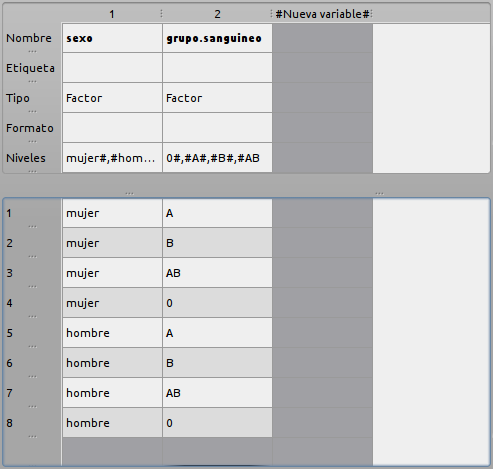
\includegraphics[scale=0.6]{probabilidad/img/espacio_muestral}
  \caption{Conjunto de datos correspondiente al espacio muestral del experimento consistente en sacar un individuo al azar de una población
  y medir su sexo y su grupo sanguíneo.}
  \label{g:espacio_muestral}
\end{center}
\end{figure}

\begin{definicion}[Suceso aleatorio]
Un \emph{suceso aleatorio} es cualquier subconjunto del espacio muestral $E$ de un experimento aleatorio. 
\end{definicion}

Existen distintos tipos de sucesos:
\begin{description}
\item[Suceso imposible:] Es el subconjunto vacío $\emptyset$. El suceso nunca ocurre.
\item[Sucesos elementales:] Son los subconjuntos formados por un solo elemento. 
\item[Sucesos compuestos:] Son los subconjuntos formados por dos o más elementos.
\item[Suceso seguro:] Es el propio espacio muestral. El suceso seguro siempre ocurre.
\end{description}

\begin{definicion}[Espacio de sucesos] Dado un espacio muestral $E$ de un
experimento aleatorio, el conjunto formado por todos los posibles sucesos de $E$ se llama \emph{espacio de sucesos de $E$} y se denota
$\mathcal{P}(E)$.
\end{definicion}

\begin{ejemplo}
Dado el espacio muestral $E=\{a,b,c\}$, se tiene 
\[
\mathcal{P}(E)=\left\{\emptyset, \{a\},\{b\},\{c\},\{a,b\},\{a,c\},\{b,c\},\{a,b,c\}\right\}
\]
\end{ejemplo}

Puesto que los sucesos son conjuntos, tiene sentido definir operaciones entre sucesos a partir de la teoría de conjuntos.

\begin{definicion}[Suceso unión]
Dados dos sucesos $A,B\in \mathcal{P}(E)$, se llama \emph{suceso unión} de $A$ y $B$, y se denota $A\cup B$, al suceso formado por los
elementos de $A$ junto a los elementos de $B$, es decir,
\[
A\cup B = \{x\,|\, x\in A\textrm{ o }x\in B\}.
\]
\begin{center}
\psset{unit=0.8}
\begin{pspicture}(-1,-1.5)(4,1.5)
\psset{fillstyle=solid}
\pscustom[fillcolor=white]{
\psframe(-1,-1.5)(4,1.5)}
\pscustom[fillcolor=yellow]{%
\psarc(1,0){1}{60}{-60}
\psarcn(2,0){1}{240}{120}}
\pscustom[fillcolor=yellow]{%
\psarc(2,0){1}{240}{120}
\psarcn(1,0){1}{60}{-60}}
\pscustom[fillcolor=yellow]{%
\psarc(1,0){1}{-60}{60}
\psarc(2,0){1}{120}{240}}
\rput(-0.7,1.2){$E$}
\rput(0.5,0){$A$}
\rput(1.5,-1.2){$A\cup B$}
\rput(2.5,0){$B$}
\end{pspicture}
\end{center}
\end{definicion}

El suceso unión $A\cup B$ ocurre siempre que ocurre $A$ \alert{o} $B$.

\begin{ejemplo}
Sea $E=\{1,2,3,4,5,6\}$, el conjunto de los números de un dado, y $A=\{2,4,6\}$ y $B=\{1,2,3,4\}$. 
Entonces $A\cup B=\{1,2,3,4,6\}$.
\end{ejemplo}

\begin{definicion}[Suceso intersección] 
Dados dos sucesos $A,B\in \mathcal{P}(E)$, se llama \emph{suceso intersección} de $A$ y $B$, y se denota $A\cap B$, al suceso formado por
los elementos comunes de $A$ y $B$, es decir, \[ A\cap B = \{x\,|\, x\in A\textrm{ y }x\in B\}.
\]
\begin{center}
\psset{unit=0.8}
\begin{pspicture}(-1,-1.5)(4,1.5)
\psset{fillstyle=solid}
\pscustom[fillcolor=white]{\psframe(-1,-1.5)(4,1.5)}
\pscustom[fillstyle=none]{%
\psarc(1,0){1}{60}{-60}
\psarcn(2,0){1}{240}{120}}
\pscustom[fillstyle=none]{%
\psarc(2,0){1}{240}{120}
\psarcn(1,0){1}{60}{-60}}
\pscustom[fillcolor=yellow]{%
\psarc(1,0){1}{-60}{60}
\psarc(2,0){1}{120}{240}}
\rput(-0.7,1.2){$E$}
\rput(0.5,0){$A$}
\rput(1.5,-1.2){$A\cap B$}
\rput(2.5,0){$B$}
\end{pspicture}
\end{center}
\end{definicion}

El suceso intersección $A\cap B$ ocurre siempre que ocurren $A$ \alert{y} $B$.

\begin{ejemplo}
Sea $E=\{1,2,3,4,5,6\}$, el conjunto de los números de un dado, y $A=\{2,4,6\}$ y $B=\{1,2,3,4\}$. 
Entonces $A\cap B=\{2,4\}$.
\end{ejemplo}

Diremos que dos sucesos son \structure{\textbf{incompatibles}} si su intersección es vacía.
Por ejemplo $A=\{2,4,6\}$ y $C=\{1,3\}$ son incompatibles.

\begin{definicion}[Suceso contrario]
Dado un conjunto $A\in \mathcal{P}(E)$, se llama \emph{suceso contrario o complementario} de $A$, y se denota $\bar A$, al suceso formado
por los elementos de $E$ que no pertenecen a $A$, es decir,
\[
\bar A = \{x\,|\, x\not\in A\}.
\]
\begin{center}
\psset{unit=0.8}
\begin{pspicture}(-1,-1.5)(4,1.5)
\psset{fillstyle=solid}
\pscustom[fillcolor=yellow]{
\psframe(-1,-1.5)(4,1.5)}
\pscustom[fillcolor=white]{%
\psarc(1,0){1}{0}{360}}
\rput(-0.7,1.2){$E$}
\rput(1,0){$A$}
\rput(3,0){$\bar A$}
\end{pspicture}
\end{center}
\end{definicion}

El suceso contrario $\bar A$ ocurre siempre que \alert{no} ocurre $A$.

\begin{ejemplo}
Sea $E=\{1,2,3,4,5,6\}$, el conjunto de los números de un dado, y $A=\{2,4,6\}$. 
Entonces $\overline A=\{1,3,5\}$.
\end{ejemplo}

\begin{definicion}[Suceso diferencia]
Dados dos sucesos $A,B\in \mathcal{P}(E)$, se llama \emph{suceso diferencia} de $A$ y $B$, y se denota $A-B$, al suceso formado por los elementos de $A$ que no pertenecen a $B$, es decir,
\[
A-B = \{x\,|\, x\in A\textrm{ y }x\not\in B\}.
\]
\begin{center}
\psset{unit=0.8}
\begin{pspicture}(-1,-1.5)(4,1.5)
\psset{fillstyle=solid}
\pscustom[fillcolor=white]{
\psframe(-1,-1.5)(4,1.5)}
\pscustom[fillcolor=yellow]{%
\psarc(1,0){1}{60}{-60}
\psarcn(2,0){1}{240}{120}}
\pscustom[fillstyle=none]{%
\psarc(2,0){1}{240}{120}
\psarcn(1,0){1}{60}{-60}}
\pscustom[fillstyle=none]{%
\psarc(1,0){1}{-60}{60}
\psarc(2,0){1}{120}{240}}
\rput(-0.7,1.2){$E$}
\rput(0.5,0){$A$}
\rput(1.5,-1.2){$A-B$}
\rput(2.5,0){$B$}
\end{pspicture}
\end{center}
\end{definicion}

El suceso diferencia $A-B$ ocurre siempre que ocurre $A$ pero no ocurre $B$, y también puede expresarse como $A\cap \bar B$.

\begin{ejemplo}
Sea $E=\{1,2,3,4,5,6\}$, el conjunto de los números de un dado, y $A=\{2,4,6\}$ y $B=\{1,2,3,4\}$. 
Entonces $A-B=\{6\}$ y $B-A=\{1,3\}$.
\end{ejemplo}

Dados los sucesos $A,B,C\in  \mathcal{P}(E)$, se cumplen las siguientes propiedades:
\begin{enumerate}
\item $A\cup A=A$, $A\cap A=A$ (idempotencia).
\item $A\cup B=B\cup A$, $A\cap B = B\cap A$ (conmutativa).
\item $(A\cup B)\cup C = A\cup (B\cup C)$, $(A\cap B)\cap C = A\cap (B\cap C)$ (asociativa).
\item $(A\cup B)\cap C = (A\cap C)\cup (B\cap C)$, $(A\cap B)\cup C = (A\cup C)\cap (B\cup C)$ (distributiva).
\item $A\cup \emptyset=A$, $A\cap E=A$ (elemento neutro).
\item $A\cup E=E$, $A\cap \emptyset=\emptyset$ (elemento absorbente).
\item $A\cup \bar A = E$, $A\cap \bar A= \emptyset$ (elemento simétrico complementario).
\item $\bar{\bar A} = A$ (doble contrario).
\item $\overline{A\cup B} = \bar A\cap \bar B$, $\overline{A\cap B} = \bar A\cup \bar B$ (leyes de Morgan).
\item $A\cap B\subseteq A\cup B$.
\end{enumerate}

\subsection{Definición de probabilidad}
En todo experimento aleatorio existe incertidumbre sobre el resultado de la realización del experimento. 
La probabilidad trata de cuantificar el grado de incertidumbre asociada a cada suceso de un experimento aleatorio. 
A lo largo de la historia se han utilizado distintas definiciones del concepto de probabilidad. 
A continuación se presentan las más comunes. 

\begin{definicion}[Probabilidad clásica de Laplace]
Para un experimento aleatorio donde todos los elementos del espacio muestral $E$ son equiprobables, se define la \emph{probabilidad} de un
suceso $A\subseteq E $ como el cociente entre el número de elementos de $A$ y el número de elementos de $E$:
\[ P(A) = \frac{|A|}{|E|} = \frac{\mbox{nº casos favorables a A}}{\mbox{nº casos posibles}}\]
\end{definicion}

\begin{ejemplo}
Si se considera el espacio muestral correspondiente al lanzamiento de un dado $E=\{1,2,3,4,5,6\}$, y el suceso correspondiente a sacar un
número par $A=\{2,4,6\}$, según la regla de Laplace, la probabilidad de sacar par al tirar un dado es
\[P(A)=\frac{|A|}{|E|}=\frac{3}{6}=0.5,\]
es decir, un 50\%. 
\end{ejemplo}

Esta definición es ampliamente utilizada, aunque tiene importantes restricciones:
\begin{itemize}[label=--]
\item No puede utilizarse con espacios muestrales infinitos, o de los que no se conoce el número de casos posibles.
\item Es necesario que todos los elementos del espacio muestral tengan la misma probabilidad de ocurrir (\emph{equiprobabilidad}).  
\end{itemize}

Estas restricciones suelen cumplirse en los experimentos relacionados con los juegos de azar (lanzamiento de dados, monedas, etc.) pero es
raro que ocurran en los experimentos de las ciencias de la salud.
Por ejemplo, los grupos sanguineos de una población humana no suelen ser equiprobables (normalmente el grupo A es mucho más probable que
el resto.)

En esto casos, y gracias al siguiente teorema, es mejor definir la probabilidad a partir de la frecuencia de cada suceso.

\begin{teorema}[Ley de los grandes números]
Cuando un experimento aleatorio se repite un gran número de veces, las frecuencias relativas de los sucesos del
experimento tienden a estabilizarse en torno a cierto número, que es precisamente su probabilidad.
\end{teorema}

Un ejemplo que demuestra el cumplimiento de esta ley puede realizarse tirando múltiples veces una moneda equilibrada y anotando la
frecuencia relativa de caras. 
A medida que se tire más veces la moneda se verá que la frecuencia relativa de caras se va estabilizando en torno a $0.5$ que es
la probabilidad de sacar cara. 

De acuerdo al teorema anterior, se puede dar la siguiente definición
\begin{definicion}[Probabilidad frecuentista]
Para un experimento aleatorio reproducible, se define la \emph{probabilidad} de un suceso $A\subseteq E $ como la frecuencia relativa del
suceso $A$ en infinitas repeticiones del experimento:
\[ P(A) = lim_{n\rightarrow \infty}\frac{n_{A}}{n}\]
\end{definicion}

\begin{ejemplo}
Si en una determinada población existe un 40\% de personas con grupo sanguíneo A, un 30\% de personas con grupo B, un 20\% con grupo 0 y un
10\% con grupo AB, de acuerdo a la definción frecuentista de probabilidad podemos decir que $P(A)=0.4$, $P(B)=0.3$, $P(0)=0.2$ y
$P(AB)=0.1$.
\end{ejemplo}

Aunque esta definición es muy útil en experimentos científicos reproducibles, también tiene serios inconvenientes, ya que
\begin{itemize}[label=--]
\item Sólo se calcula una aproximación de la probabilidad real.
\item La repetición del experimento debe ser en las mismas condiciones.  
\end{itemize}

No fue hasta el siglo XX cuando Kolmogórov dió una definición de probabilidad que unificaba las anteriores y que actualmente es la más
aceptada.

\begin{definicion}[Kolmogórov]
Se llama \emph{probabilidad} a toda aplicación que asocia a cada suceso $A$ del espacio de sucesos de un experimento aleatorio, un número
real $P(A)$, que cumple los siguientes axiomas:
\begin{enumerate}
\item La probabilidad de un suceso cualquiera es positiva o nula: \[P(A)\geq 0.\]
\item La probabilidad de la unión de dos sucesos incompatibles es igual a la suma de las probabilidades de cada uno de ellos:       
\[P(A\cup B) = P(A)+P(B).\]
\item La probabilidad del suceso seguro es igual a la unidad: 
\[P(E)=1.\]
\end{enumerate}
\end{definicion}

A partir de los axiomas de la definición de probabilidad se pueden deducir los siguientes resultados:
\begin{enumerate}
\item $P(\bar A) = 1-P(A)$.
\item $P(\emptyset)= 0$.
\item Si $A\subseteq B$ entonces $P(A)\leq P(B)$.
\item $P(A) \leq 1$.
\item Si $A$ y $B$ son sucesos compatibles, es decir, su intersección no es vacía, entonces 
\[P(A\cup B)= P(A) + P(B) - P(A\cap B).\]
\item Si el suceso $A$ está compuesto por los sucesos elementales $e_1,e_2,...,e_n$, entonces 
\[P(A)=\sum_{i=1}^n P(e_i).\]
\end{enumerate}

Este último resultado es especialmente interesante, pues pemite calcular la probabilidad de cualquier suceso de manera muy sencilla
simplemente sumando las probabilidades de los elementos que lo componen. 

\subsection{Probabilidad condicionada}
La incertidumbre sobre un suceso depende de la información que se tenga sobre el experimento aleatorio. 
En algunas ocasiones puede que haya que calcular la probabilidad de algún suceso $A$ sabiendo que ha ocurrido otro $B$. 
En tal caso se dice que el suceso $B$ es un \emph{condicionante}, y la probabilidad del suceso condicionado suele escribirse como 
\[P(A/B)\]

Los condicionantes, en el fondo, cambian el espacio muestral del experimento y por tanto las probabilidades de sus sucesos.

\begin{ejemplo}
Supongamos que hemos observado las siguientes frecuencias de fumadores en un grupo de 100 hombres y 100 mujeres:
\[
\begin{array}{|c|c|c|}
\cline{2-3}
 \multicolumn{1}{c|}{} & \mbox{Fuma} & \mbox{No Fuma} \\ \hline 
 \mbox{Mujeres} & 30 & 70 \\ \hline
 \mbox{Hombres} & 40 & 60 \\ \hline
 \mbox{Total} & 70 & 130 \\ \hline
\end{array}
\]
Entonces, utilizando la definición de frecuentista, la probabilidad de que una persona elegida al azar sea fumadora es
la frecuencia relativa de fumar que es $P(\mbox{Fumar})= 70/200=0.35$.

Sin embargo, si se añade información sobre el experimento y nos dicen que la persona elegida es mujer, entonces la muestra se restringiría
sólo a las mujeres y la frecuencia relativa de fumar en mujeres es $P(\mbox{Fumar}/\mbox{Mujer})=30/100=0.3$. 
\end{ejemplo}

El problema de los condicionamientos es que suelen cambiar el espacio muestral de partida. 
Afortunadamente, es posible calcular probabilidades condicionadas sin cambiar de espacio muestral gracias a la siguiente fórmula.

\begin{definicion}[Probabilidad condicionada]
Dados dos sucesos $A$ y $B$ de un mismo espacio de sucesos de un experimento aleatorio, la probabilidad de $A$ \emph{condicionada} por $B$
es 
\[ P(A/B) = \frac{P(A\cap B)}{P(B)},\]
siempre y cuando, $P(B)\neq 0$.
\end{definicion}

Esta definición permite calcular probabilidades sin tener que alterar el espacio muestral original del experimento.

\begin{ejemplo}
Siguiendo con el anterior, si se calcula la probabilidad de fumar en el caso de ser mujer con esta fórmula se obitne el mismo resultado:
\[P(\mbox{Fumar}/\mbox{Mujer})= \frac{P(\mbox{Fumar}\cap \mbox{Mujer})}{P(\mbox{Mujer})} = \frac{30/200}{100/200}=\frac{30}{100}=0.3.\]
\end{ejemplo}

De esta definición se deduce que la probabilidad de la intersección es
\[ P(A\cap B) = P(A)P(B/A) = P(B)P(A/B).\]

En ocasiones, saber que un determinado suceso ha ocurrido no cambia la incertidumbre sobre otro suceso del mismo experimento. 
Por ejemplo, si se tiran dos monedas, está claro que el resultado de la primera no cambia la incertidumbre sobre el resultado de la segunda.
En tal caso se dice que los sucesos son independientes.

\begin{definicion}[Sucesos independientes]
Dados dos sucesos $A$ y $B$ de un mismo espacio de sucesos de un experimento aleatorio, se dice que $A$ es \emph{independiente} de $B$, si
la probabilidad de $A$ no se ve alterada al condicionar por $B$, es decir,
\[ P(A/B) = P(A).\]
\end{definicion}

Si $A$ es independiente de $B$, también se cumple que $B$ es independiente de $A$, y en general simplemente se dice que $A$ y $B$ son
independientes.

También se cumple que si $A$ y $B$ son independientes, entonces 
\[ P(A\cap B) = P(A)P(B/A) = P(A)P(B). \]


\subsection{Espacios probabilísticos}
Si a cada uno de los elementos del espacio muestral de un experimento se le asocia su probabilidad, se obtiene un \emph{espacio
probabilístico}.

Resulta sencillo construir espacios probabilísticos a partir de los diagramas de árbol que se vieron para construir espacios muestrales. 
Para ello se deben etiquetar las ramas del árbol con probabilidades del siguiente modo: 
\begin{enumerate}
\item Para cada nodo del árbol, etiquetar su rama con la probabilidad de que la variable correspondiente tome el valor del nodo,
condicionada por la ocurrencia de todos los nodos que conducen hasta el actual.
\item La probabilidad de cada suceso elemental se calcula multiplicando las probabilidades que etiquetan las ramas que
conducen hasta él.
\end{enumerate}

\begin{ejemplo}[Espacio probabilístico con variables dependientes]
Sea una población en la que el 30\% de las personas fuman, y que la incidencia del cáncer de pulmón en fumadores es del 40\% mientras que 
en los no fumadores es del 10\%.

El espacio probabilístico de este experimento es:

\begin{center}
\psset{treesep=0.6cm, levelsep=3.5cm, tpos=0.6}
\renewcommand{\psedge}[2]{\ncdiag[armA=1.2cm,angleA=180,angleB=0,armB=0cm]{#2}{#1}} 
\pstree[treemode=R, nodesep=1pt]{\Tp*}{
	\pstree[linestyle=none]{\TR[edge=none]{Tabaco}}{
		\pstree{\TR{Enfermedad}}{
			\pstree{\TR{$E$}}{\TR{$P$}}
		}
	}
	\pstree{\TR{Fuma}\taput{\scriptsize $P(F)=0.3$}}{
		\pstree[linestyle=none]{\TR{Cáncer}\taput{\scriptsize $P(C/F)=0.4$}}{
			\pstree{\TR{(Fuma,Cáncer)}}{\TR{$0.3\cdot 0.4 = 0.12$}}
		}
		\pstree[linestyle=none]{\TR{$\overline{\mbox{Cáncer}}$}\taput{\scriptsize $P(\bar C/F)=0.6$}}{
			\pstree{\TR{(Fuma,$\overline{\mbox{Cáncer}}$)}}{\TR{$0.3\cdot 0.6 = 0.18$}}
		}
	}
	\pstree{\TR{$\overline{\mbox{Fuma}}$}\taput{\scriptsize $P(\bar F)=0.7$}}{
		\pstree[linestyle=none]{\TR{Cáncer}\taput{\scriptsize $P(C/\bar F)=0.1$}}{
			\pstree{\TR{($\overline{\mbox{Fuma}}$,Cáncer)}}{\TR{$0.7\cdot 0.1 = 0.07$}}
		}
		\pstree[linestyle=none]{\TR{$\overline{\mbox{Cáncer}}$}\taput{\scriptsize $P(\bar C/\bar F)=0.9$}}{
			\pstree{\TR{($\overline{\mbox{Fuma}}$,$\overline{\mbox{Cáncer}}$)}}{\TR{$0.7\cdot 0.9 = 0.63$}}
		}
	}
	\pstree[linestyle=none]{\Tp[edge=none]}{\Tp}
}
\end{center}

Obsérvese que el fumar o no depende del sexo, así que las ramas que salen del suceso mujer no tienen las mismas probabilidades que las que
salen del suceso hombre.
\end{ejemplo}

Cuando las variables observadas en el experimento son independientes, la construcción del espacio probabilístico se simplifica, ya que las
probabilidades condicionadas se convierten en probabilidades simples.

\begin{ejemplo}[Espacio probabilístico con variables independientes]
El espacio probabilístico del experimento aleatorio que consiste en el lanzamiento de dos monedas es:

\begin{center}
\psset{treesep=0.6cm, levelsep=2.5cm, tpos=0.7}
\renewcommand{\psedge}[2]{\ncdiag[armA=0.8cm,angleA=180,angleB=0,armB=0cm]{#2}{#1}} 
\pstree[treemode=R, nodesep=1pt]{\Tp*}{
	\pstree[linestyle=none]{\TR[edge=none]{1ª Moneda}}{\pstree{\TR{2ª Moneda}}{\pstree{\TR{$E$}}{\TR{$P$}}}}
	\pstree{\TR{C}\taput{\scriptsize $0.5$}}{
		\pstree[linestyle=none]{\TR{C}\taput{\scriptsize $0.5$}}{\pstree{\TR{(C,C)}}{\TR{$0.5\cdot 0.5 = 0.25$}}}
		\pstree[linestyle=none]{\TR{X}\taput{\scriptsize $0.5$}}{\pstree{\TR{(C,X)}}{\TR{$0.5\cdot 0.5 = 0.25$}}}
	}
	\pstree{\TR{X}\taput{\scriptsize $0.5$}}{
		\pstree[linestyle=none]{\TR{C}\taput{\scriptsize $0.5$}}{\pstree{\TR{(X,C)}}{\TR{$0.5\cdot 0.5 = 0.25$}}}
		\pstree[linestyle=none]{\TR{X}\taput{\scriptsize $0.5$}}{\pstree{\TR{(X,X)}}{\TR{$0.5\cdot 0.5 = 0.25$}}}
	}
	\pstree[linestyle=none]{\Tp[edge=none]}{\Tp}
}
\end{center}

Obsérvese ahora que el resultado de la segunda moneda no depende del resultado de la primera, de manera que las ramas que salen del suceso
cara en la primera moneda tienen las mismas probabilidades que las que salen del suceso cruz.
\end{ejemplo}  


\subsection{Teorema de la probabilidad total}
En algunos experimentos es posible descomponer el espacio muestral en partes que forman un sistema completo de sucesos. 

\begin{definicion}[Sistema completo de sucesos]
Una colección de sucesos $A_1,A_2,\ldots,A_n$ de un mismo espacio de sucesos es un \emph{sistema completo} si cumple las siguientes condiciones:
\begin{enumerate}
\item La unión de todos es el espacio muestral: $A_1\cup \cdots\cup A_n =E$.
\item Son incompatibles dos a dos: $A_i\cap A_j = \emptyset$ $\forall i\neq j$.
\end{enumerate}
\end{definicion}
\begin{center}
\psset{unit=0.8}
\begin{pspicture}(0,0)(5,3.5)
\psset{fillstyle=solid}
\pscustom[fillcolor=white]{\psframe(0,0)(5,3)}
\psline(1,0)(1,3)
\psline(2,0)(2,3)
\psline(4,0)(4,3)
\rput(0.5,1.5){$A_1$}
\rput(1.5,1.5){$A_2$}
\rput(3,1.5){$\cdots$}
\rput(4.5,1.5){$A_n$}
\rput[b](0.2,3.2){$E$}
\end{pspicture}
\end{center}

En realidad un sistema completo de sucesos es una partición del espacio muestral de acuerdo a algún atributo, como por ejemplo el sexo o el
grupo sanguíneo.

Conocer las probabilidades de un determinado suceso en cada una de las partes de un sistema completo puede ser útil para calcular su
probabilidad a partir del siguiente teorema.

\begin{teorema}[Probabilidad total]
Dado un sistema completo de sucesos $A_1,\ldots,A_n$ y un suceso $B$ de un mismo espacio de sucesos, se cumple
\[
P(B) = \sum_{i=1}^n P(A_i)P(B/A_i).
\]
\end{teorema}

\begin{center}
\psset{unit=1}
\begin{pspicture}(0,0)(5,3.5)
\psset{fillstyle=solid}
\pscustom[fillcolor=white]{\psframe(0,0)(5,3)}
\pscustom[fillcolor=coral]{\psellipse(2.5,1.5)(2,1)}
\psline(1,0)(1,3)
\psline(2,0)(2,3)
\psline(4,0)(4,3)
\rput(0.5,0.2){$A_1$}
\rput(1.5,0.2){$A_2$}
\rput(3,0.2){$\cdots$}
\rput(4.5,0.2){$A_n$}
\rput(3,1.5){$B$}
\rput[b](0.2,3.2){$E$}
\end{pspicture}
\end{center}

\begin{ejemplo}
Un determinado síntoma $B$ puede ser originado por una enfermedad $A$ pero también lo pueden presentar las personas sin
la enfermedad. 
Se sabe que en la población la tasa de personas con la enfermedad A es $0.2$. 
Además, de las personas que presentan la enfermedad, el $90\%$ presentan el síntoma, mientras que de las personas sin la enfermedad sólo lo
presentan el $40\%$.

Si se toma una persona al azar de la población, \emph{¿qué probabilidad hay de que tenga el síntoma?}

Para responder a la pregunta hay que fijarse en que el conjunto de sucesos $\{A,\bar A\}$ es un sistema completo, ya que $A\cup
\bar A = E$ y $A\cap \bar A = \emptyset$, de modo que se puede aplicar el teorema de la probabilidad total se tiene
\[ P(B) = P(A)P(B/A)+P(\bar A)P(B/\bar A) = 0.2\cdot 0.9 + 0.8\cdot 0.4 = 0.5.\] 
Es decir, la mitad de la población tendrá el síntoma.

En el fondo se trata de una media ponderada de probabilidades. 

La respuesta a la pregunta anterior es evidente a la luz del espacio probabilístico del experimento. 
\begin{center}
\psset{treesep=0.6cm, levelsep=2.5cm, tpos=0.6}
\renewcommand{\psedge}[2]{\ncdiag[armA=0.8cm,angleA=180,angleB=0,armB=0cm]{#2}{#1}} 
\pstree[treemode=R, nodesep=1pt]{\Tp*}{
	\pstree[linestyle=none]{\TR[edge=none]{Enfermedad}}{
		\pstree{\TR{Síntoma}}{
			\pstree{\TR{$E$}}{\TR{$P$}}
		}
	}
	\pstree{\TR{$A$}\taput{\scriptsize $0.2$}}{
		\pstree[linestyle=none]{\TR{$B$}\taput{\scriptsize $0.9$}}{
			\pstree{\TR{\alert{$(A,B)$}}}{\TR{\alert{$0.2\cdot 0.9 = 0.18$}}}
		}
		\pstree[linestyle=none]{\TR{$\bar B$}\taput{\scriptsize $0.1$}}{
			\pstree{\TR{$(A,\bar B)$}}{\TR{$0.2\cdot 0.1 = 0.02$}}
		}
	}
	\pstree{\TR{$\bar A$}\taput{\scriptsize $0.8$}}{
		\pstree[linestyle=none]{\TR{$B$}\taput{\scriptsize $0.4$}}{
			\pstree{\TR{\alert{$(\bar A,B)$}}}{\TR{\alert{$0.8\cdot 0.4 = 0.32$}}}
		}
		\pstree[linestyle=none]{\TR{$\bar B$}\taput{\scriptsize $0.6$}}{
			\pstree{\TR{$(\bar A,\bar B)$}}{\TR{$0.8\cdot 0.6 = 0.48$}}
		}
	}
	\pstree[linestyle=none]{\Tp[edge=none]}{\Tp}
}
\end{center}
\[
P(B) = P(A,B) + P(\bar A,B) = P(A)P(B/A)+P(\bar A)P(B/\bar A) = 0.2\cdot 0.9+ 0.8\cdot 0.4 = 0.18 + 0.32 = 0.5. 
\]
\end{ejemplo}


\subsection{Teorema de Bayes}
Los sucesos de un sistema completo de sucesos $A_1,\cdots,A_n$ también pueden verse como las distintas hipótesis ante un determinado hecho
$B$.

En estas condiciones puede ser útil calcular las probabilidades a posteriori $P(A_i/B)$ de cada una de las hipótesis, es decir, una vez
se haya cumplido el suceso $B$. 
Para ello se utiliza el teorema de Bayes. 

\begin{teorema}[Bayes]
Dado un sistema completo de sucesos $A_1,\ldots,A_n$ y un suceso $B$ de un mismo espacio de sucesos, se cumple
\[
P(A_i/B) = \frac{P(A_i\cap B)}{P(B)} = \frac{P(A_i)P(B/A_i)}{\sum_{i=1}^n P(A_i)P(B/A_i)}.
\]
\end{teorema}

\begin{ejemplo}[Diagnóstico de una enfermedad]
En el ejemplo anterior se ha visto cómo calcular la probabilidad de que una persona elegida al azar presente el síntoma, pero desde un 
punto de vista de diagnóstico clínico es mucho más interesante calcular la probabilidad de que una persona que presenta el síntoma tenga la
enfermedad, ya que esto permitiría diagnosticar la enfermedad o descartarla. 

En este caso, las hipótesis ante las que hay que decidir son $A$ y $\bar A$ y sus probabilidades ``a priori'' son $P(A)=0.2$ y
$P(\bar A)=0.8$.

Esto quiere decir que si no hubiese ninguna información sobre la persona, el diagnóstico sería que no tiene la enfermedad pues es mucho más
probable que que la tenga.

Sin embargo, si al reconocer a la persona se observa que presenta el síntoma, dicha información condiciona a las hipótesis, y para decidir
entre ellas es necesario calcular sus probabilidades ``a posteriori'', es decir 
\[ P(A/B) \mbox{ y } P(\bar A/B)\]

Para calcular estas probabilidades se puede utilizar el teorema de Bayes.
\begin{align*}
P(A/B) &= \frac{P(A)P(B/A)}{P(A)P(B/A)+P(\bar A)P(B/\bar A)} = \frac{0.2\cdot 0.9}{0.2\cdot 0.9 + 0.8\cdot 0.4} =
\frac{0.18}{0.5}=0.36,\\
P(\bar A/B) &= \frac{P(\bar A)P(B/\bar A)}{P(A)P(B/A)+P(\bar A)P(B/\bar A)} = \frac{0.8\cdot 0.4}{0.2\cdot 0.9 +
0.8\cdot 0.4} = \frac{0.32}{0.5}=0.64.
\end{align*}
Según esto, a pesar de que la probabilidad de estar enfermo ha aumentado, seguiríamos diagnosticando que no lo está, puesto que es más
probable.

En este caso se dice que el síntoma $B$ \emph{no es determinante} a la hora de diagnosticar la enfermedad, pues la información que aporta no
sirve para cambiar el diagnóstico en ningún caso.
\end{ejemplo}


\subsection{Tests diagnósticos}
En epidemiología es común el uso de tests para diagnosticar enfermedades.

Generalmente estos tests no son totalmente fiables, sino que hay cierta probabilidad de acierto o fallo en el diagnóstico, que suele
representarse en la siguiente tabla:
\begin{center}
\begin{tabular}{|m{3cm}<{\centering}|m{3.5cm}<{\centering}|m{3.5cm}<{\centering}|}
\cline{2-3}
\multicolumn{1}{c|}{} & Presencia de la\newline enfermedad ($E$) & Ausencia de la\newline enfermedad ($\overline E$)\\ \hline
Test positivo\newline ($+$) & \textcolor{green}{Diagnóstico acertado\newline  $P(+/E)$}\qquad
\structure{Sensibilidad}& \textcolor{red}{Diagnóstico erróneo\newline $P(+/\overline E)$}\\ \hline Test negativo\newline ($-$) &
\textcolor{red}{Diagnóstico erróneo\newline $P(-/E)$} & \textcolor{green}{Diagnóstico acertado\newline $P(-/\overline
E)$}\qquad \structure{Especificidad}\\ \hline
\end{tabular}
\end{center}

La valided de una prueba diagnóstica depende de estas dos probabilidades:
\begin{description}
\item[\textbf{Sensibilidad}] Es el porcentaje de positivos entre las personas enfermas: $P(+/E)$.
\item[\textbf{Especificidad}] Es el porcentaje de negativos entre las personas sanas: $P(-/\bar E)$.
\end{description}

Pero lo realmente interesante de un un test diagnóstico es su capacidad predictiva para diagnosticar, lo cual se mide mediante las
siguientes probabilidades a posteriori:
\begin{description}
\item[\textbf{Valor predictivo positivo}] Es el porcentaje de enfermos entre los positivos: $P(E/+)$.
\item[\textbf{Valor predictivo negativo}] Es el porcentaje de sanos entre los negativos: $P(\bar E/-)$.
\end{description}

Sin embargo, estos últmos valores dependen del porcentaje de enfermos en la población $P(E)$, lo que se conoce como, \emph{tasa
o prevalencia} de la enfermedad.

\begin{ejemplo}
Un test para diagnosticar la gripe tiene una sensibilidad del $95\%$ y una especificidad del $90\%$. 
Según esto, las probabilidades de
acierto y fallo del test son:
\begin{center}
\begin{tabular}{|c|c|c|}
\cline{2-3}
\multicolumn{1}{c|}{} & Gripe & No gripe\\ \hline
Test $+$ & $0.95$ & $0.10$\\ \hline
Test $-$ & $0.05$ & $0.90$\\ \hline
\end{tabular}
\end{center}

Si la prevalencia de la gripe en la población es del $10\%$ y al aplicar el test a un individuo da positivo, \emph{¿cuál es la probabilidad
de que tenga gripe?}

Aplicando el teorema de Bayes, se tiene que el valor predictivo positivo del test vale
\[
P(\mbox{Gripe}/+) = \frac{P(\mbox{Gripe})P(+/\mbox{Gripe})}{P(\mbox{Gripe})P(+/\mbox{Gripe})+P(\overline{\mbox{Gripe}})P(+/\overline{\mbox{Gripe}})}
= \frac{0.1\cdot 0.95}{0.1\cdot 0.95+0.9\cdot 0.1} = 0.5135.
\]
La probabilidad de no tener la gripe sería $P(\overline{\mbox{Gripe}})=1-0.51=0.49$, y como la probabilidad de tener la gripe es mayor que
la de no tenerla, se diagnosticaría que tiene gripe.
Sin embargo, el valor predictivo positivo de este test es muy bajo y nos equivoaríamos en el 49\% de los diagnósticos de enfermedad.

Y si el test da negativo, \emph{¿cuál es la probabilidad de que no tenga gripe?}

De nuevo, aplicando el teorema de Bayes, se tiene que el valor predictivo negativo del test vale
\[
P(\overline{\mbox{Gripe}}/-)=
\frac{P(\overline{\mbox{Gripe}})P(-/\overline{\mbox{Gripe}})}{P(\mbox{Gripe})P(-/\mbox{Gripe})+P(\overline{\mbox{Gripe}})P(-/\overline{\mbox{Gripe}})}
= \frac{0.9\cdot 0.9}{0.1\cdot 0.05+0.9\cdot 0.9} = 0.9939.
\]
De manera que el valor predictivo negativo de este test es mucho más alto que el valor predictivo positivo, y por tanto este test es mucho
más útil para descartar la enfermedad que para detectarla.
\end{ejemplo}


\clearpage
\newpage

\section{Ejercicios resueltos}
\begin{enumerate}[leftmargin=*] 
\item Construir los espacios probabilísticos correspondientes a los siguientes experimentos aleatorios:
\begin{enumerate}
\item Sacar una carta de una baraja española.
\begin{indicacion}
\begin{enumerate}
\item Seleccionar el menú \menu{Teaching > Probabilidad > Juegos de azar > Naipes > Espacio probabilístico}.
\item En el cuadro de diálogo que aparece y hacer clic en el botón \boton{Enviar}. 
\end{enumerate}
\end{indicacion}
\item Lanzar dos monedas.
\begin{indicacion}
\begin{enumerate}
\item Seleccionar el menú \menu{Teaching > Probabilidad > Juegos de azar > Monedas > Espacio probabilístico}.
\item En el cuadro de diálogo que aparece, introducir 2 en el campo \campo{Número de monedas} y hacer clic en el botón \boton{Enviar}.
\end{enumerate}
\end{indicacion}

\item Lanzar dos dados.
\begin{indicacion}
\begin{enumerate}
\item Seleccionar el menú \menu{Teaching > Probabilidad > Juegos de azar > Dados > Espacio probabilístico}.
\item En el cuadro de diálogo que aparece, introducir 2 en el campo \campo{Número de dados} y hacer clic en el botón \boton{Enviar}.
\end{enumerate}
\end{indicacion}

\item Lanzar dos dados y dos monedas. 
\begin{indicacion}
\begin{enumerate}
\item Seleccionar el menú \menu{Teaching > Probabilidad > Combinar espacios probabi\-lís\-ticos independientes}.
\item En el cuadro de diálogo que aparece, seleccionar los conjuntos de datos correspondientes a los espacios muestrales del lanzamiento de
dos monedas y del lanzamiento de dos dados generados en los apartados anteriores, y hacer clic en el botón \boton{Enviar}.
\end{enumerate}
\end{indicacion}
\end{enumerate}  

\item Repetir el experimento de lanzar dos monedas 10 veces, 100 veces, 1000 veces y 1000000 de veces y calcular las frecuencias relativas
de cada resultado. 
¿Hacia dónde tienden las frecuencias? 
Construir el espacio probabilístico de este experimento y comprobar que se cumple la ley de los grandes números, es decir, que las
frecuencias anteriores se aproximan a las probabilidades de cada suceso elemental.
\begin{indicacion}
Para la realización del experimento:
\begin{enumerate}
\item Seleccionar el menú \menu{Teaching > Probabilidad > Juegos de azar > Monedas > Lanzamiento de monedas}.
\item En el cuadro de diálogo que aparece, introducir 2 en el campo \campo{Número de monedas}, introducir 10 en el campo \campo{Número de
lanzamientos}, activar la casilla \opcion{Distribución de frecuencias} y hacer clic en el botón \boton{Enviar}.
\end{enumerate}
Repetir los mismos pasos pero introduciendo 100, 1000 y 1000000 respectivamente en el campo \opcion{Número de lanzamientos}.

Para construir el espacio probabilístico correspondiente:
\begin{enumerate}
\item Seleccionar el menú \menu{Teaching > Probabilidad > Juegos de azar > Monedas > Espacio probabilístico}.
\item En el cuadro de diálogo que aparece, introducir 2 en el campo \campo{Número de monedas} y hacer clic en el botón \boton{Enviar}.
\end{enumerate}
\end{indicacion}

\item En una estantería hay tres cajas de un medicamento A, dos de un medicamento B y una de un medicamento C. 
Construir los espacios probabilísticos asociados a los siguientes experimentos aleatorios:
\begin{enumerate}
\item Elegir tres medicamentos al azar sin reemplazamiento. 
\begin{indicacion}
\begin{enumerate}
\item Seleccionar el menú \menu{Teaching > Probabilidad > Juegos de azar > Urna > Espacio probabilístico}.
\item En el cuadro de diálogo que aparece, seleccionar la opción \opcion{Lista de objetos}, introducir los objetos A,A,A,B,B,C en
el campo \campo{Lista de objetos}, introducir 3 en el campo \campo{Número de extracciones}, y hacer clic en el botón \boton{Enviar}.
\end{enumerate}
\end{indicacion}

\item Elegir tres medicamentos al azar con reemplazamiento.
\begin{indicacion}
Repetir los mismos pasos del apartado anterior pero además activando la casilla \opcion{Con reemplazamiento}.
\end{indicacion}
\end{enumerate}

\opt{largo}{\item Gregor Mendel, monje austríaco, desarrollo en el siglo XIX los principios fundamentales de genética.
Mendel demostró que las características heredables se transmiten en unidades discretas que se heredan por separado en cada generación.
Estas unidades discretas, que Mendel llamó \emph{elemente}, se conocen hoy como \emph{genes}.

Cada característica hereditaria depende de dos factores separados que provienen uno de cada progenitor.
Estos factores son los \emph{alelos} de cada gen, que pueden ser \emph{dominantes} (cuando se expresan en el fenotipo sin tener en cuenta el
otro alelo) o \emph{recesivos} (que se expresa sólo cuando el otro alelo es igual).

Mendel demostró que en la reproducción los alelos se combinan aleatoriamente y de manera independiente para formar el gen del hijo.

En uno de sus experimentos cruzó dos plantas de gisantes con idéntico genotipo Aa y Bb, donde el primer gen se refiere al color del guisante
(A amarillo y a verde) y el segundo gen se refiere a la forma del guisante (B liso y b rugoso). Se pide:
\begin{enumerate}
\item Construir el espacio probabilístico correspondiente al genotipo del gen del color. 
¿Cuál es la probabilidad que la planta resultante diese guisantes con fenotipo amarillo? 
¿Y verde?
\begin{indicacion}
Para construir el espacio probabilístico: 
\begin{enumerate}
\item Crear un conjunto de datos \variable{mendel.color} con la variable \variable{alelo.color.progenitor} con los dos posibles alelos del
progenitor correspondientes al gen del color (A y a).
\item Seleccionar el menú \menu{Teaching > Probabilidad > Construir espacio probabi\-lís\-tico}.
\item En el cuadro de diálogo que aparece seleccionar el conjunto de datos \variable{mendel.color}, darle el nombre
\variable{mendel.color.ep} al espacio probabilístico y hacer clic en el botón \boton{Enviar}.
\item Seleccionar el menú \menu{Teaching > Probabilidad > Repetir espacio probabilís\-ti\-co}.
\item En el cuadro de diálogo que aparece seleccionar el conjunto de datos \variable{mendel.color.ep}, introducir 2 en el campo
\campo{Número de repeticiones}, darle el mismo nombre al espacio probabilístico resultante y hacer clic en el botón \boton{Enviar}. 
\end{enumerate}
Para calcular la probabilidad de fenotipo amarillo:
\begin{enumerate}
\item Seleccionar el menú \menu{Teaching > Probabilidad > Calcular probabilidad}.
\item En el cuadro de diálogo que aparece seleccionar el espacio probabilístico \variable{mendel.color.ep}, introducir
\comando{alelo.color.progenitor.1 == "\mbox{A}"\ | alelo.color.pro\-genitor.2 == "\mbox{A}"} en el campo \campo{Suceso} y hacer clic en el
botón \boton{Enviar}.
\end{enumerate}
Para calcular la probabilidad de fenotipo verde:
\begin{enumerate}
\item Seleccionar el menú \menu{Teaching > Probabilidad > Calcular probabilidad}.
\item En el cuadro de diálogo que aparece seleccionar el espacio probabilístico \variable{mendel.color.ep}, introducir
\comando{alelo.color.progenitor.1 == "\mbox{a}"\ \& alelo.color.pro\-genitor.2 == "\mbox{a}"} en el campo \campo{Suceso} y hacer clic en el
botón \boton{Enviar}.
\end{enumerate}
\end{indicacion}

\item Construir el espacio probabilístico correspondiente al genotipo de ambos genes. 
¿Cuál es la probabilidad que la planta resultante diese guisantes con fenotipo amarillo y liso? 
¿Y verde y rugoso?
\begin{indicacion}
Para construir el espacio probabilístico: 
\begin{enumerate}
\item Crear un conjunto de datos \variable{mendel.forma} con la variable \variable{alelo.forma.progenitor} con los dos posibles alelos del
progenitor correspondientes al gen de la forma (B y b).
\item Seleccionar el menú \menu{Teaching > Probabilidad > Construir espacio probabilístico}.
\item En el cuadro de diálogo que aparece seleccionar el conjunto de datos \variable{mendel.forma}, darle el nombre
\variable{mendel.forma.ep} al espacio probabilístico y hacer clic en el botón \boton{Enviar}.
\item Seleccionar el menú \menu{Teaching > Probabilidad > Repetición de espacio probabilístico}.
\item En el cuadro de diálogo que aparece seleccionar el conjunto de datos \variable{mendel.forma.ep}, darle el mismo nombre al espacio
probabilístico resultante y hacer clic en el botón \boton{Enviar}. 
\item Seleccionar el menú \menu{Teaching > Probabilidad > Combinación de espacios probabilísticos independientes}.
\item En el cuadro de diálogo que aparece, seleccionar los conjuntos de datos correspondientes a los espacios probalísticos
\variable{mendel.color.ep} y \variable{mendel.forma.ep},  darle el nombre \variable{mendel.color.forma.ep} al espacio
probabilístico resultante y hacer clic en el botón \boton{Enviar}.
\end{enumerate}
Para calcular la probabilidad de fenotipo amarillo y liso:
\begin{enumerate}
\item Seleccionar el menú \menu{Teaching > Probabilidad > Calcular probabilidad}.
\item En el cuadro de diálogo que aparece seleccionar el espacio probabilístico \variable{mendel.color.forma.ep}, introducir
\comando{(alelo.color.progenitor.1 == "\mbox{A}"\ | alelo.color.\-pro\-genitor.2 == "\mbox{A}")\ \& (alelo.forma.progenitor.1 == "B"\ |
alelo.for\-ma.\-pro\-genitor.2 == "B")} en el campo \campo{Suceso}, y hacer clic en el botón \boton{Enviar}.
\end{enumerate}
Para calcular la probabilidad de fenotipo verde y rugoso:
\begin{enumerate}
\item Seleccionar el menú \menu{Teaching > Probabilidad > Calcular probabilidad}.
\item En el cuadro de diálogo que aparece seleccionar el espacio probabilístico \variable{mendel.color.forma.ep}, introducir
\comando{alelo.color.progenitor.1 == "\mbox{a}"\ \& alelo.color.\-pro\-genitor.2 == "\mbox{a}"\ \& alelo.forma.progenitor.1== "\mbox{b}"\ \&
alelo.forma.\-progenitor.2 == "\mbox{b}"} en el campo \campo{Suceso} y hacer clic en el botón \boton{Enviar}.
\end{enumerate}
\end{indicacion}
\end{enumerate}
}

\item En una población se ha hecho un estudio epidemiológico sobre tres enfermedades asociadas habitualmente a la infancia, como son la
varicela, el sarampión y la rubeola.
Las frecuencias observadas aparecen en la siguiente tabla:
\begin{center} 
\begin{tabular}{cccr}
\hline
Varicela & Sarampión & Rubeola & Frecuencia\\
No & No & No & 2654\\
No & No & Si & 1436\\
No & Si & No & 1682\\
No & Si & Si & 668\\
Si & No & No & 1747\\
Si & No & Si & 476\\
Si & Si & No & 876\\
Si & Si & Si & 265\\
\hline
\end{tabular}
\end{center}

Se pide:
\begin{enumerate}
\item Crear el conjunto de datos \variable{enfermedades.infantiles} con las variables \variable{varicela}, \variable{sarampion},
\variable{rubeola} y \variable{frecuencia} e introducir datos de la población.

\item Crear el espacio probabilístico asociado a la población.
\begin{indicacion}
\begin{enumerate}
\item Seleccionar el menú \menu{Teaching > Probabilidad > Construir espacio probabi\-lís\-tico}.
\item En el cuadro de diálogo que aparece seleccionar el conjunto de datos \variable{enfermedades.infantiles}, activar la casilla
\opcion{Definir frecuencias}, seleccionar la variable \variable{frecuencia} en el campo \campo{Frecuencia}, darle el nombre
\variable{enfermedades.infantiles.ep} al espacio probabilístico y hacer clic en el botón \boton{Enviar}.
\end{enumerate}
\end{indicacion}  

\item Calcular la probabilidad de que una persona de esta población haya tenido varicela. 
\begin{indicacion}
\begin{enumerate}
\item Seleccionar el menú \menu{Teaching > Probabilidad > Calcular probabilidad}.
\item En el cuadro de diálogo que aparece seleccionar el espacio probabilístico \variable{enfermedades.infantiles.ep}, introducir
\comando{varicela == "Si"} en el campo \campo{Suceso} y hacer clic en el botón \boton{Enviar}.
\end{enumerate}
\end{indicacion} 

\item Calcular la probabilidad de que una persona de esta población haya tenido varicela o sarampión. 
\begin{indicacion}
\begin{enumerate}
\item Seleccionar el menú \menu{Teaching > Probabilidad > Calcular probabilidad}.
\item En el cuadro de diálogo que aparece seleccionar el espacio probabilístico \variable{enfermedades.infantiles.ep}, introducir
\comando{varicela == "Si"\ | sarampion=="Si"} en el campo \campo{Suceso} y hacer clic en el botón \boton{Enviar}.
\end{enumerate}
\end{indicacion} 

\item Calcular la probabilidad de que una persona de esta población haya tenido sarampión y rubeola. 
\begin{indicacion}
\begin{enumerate}
\item Seleccionar el menú \menu{Teaching > Probabilidad > Calcular probabilidad}.
\item En el cuadro de diálogo que aparece seleccionar el espacio probabilístico \variable{enfermedades.infantiles.ep}, introducir
\comando{sarampion == "Si"\ \& rubeola=="Si"} en el campo \campo{Suceso} y hacer clic en el botón \boton{Enviar}.
\end{enumerate}
\end{indicacion} 

\item Calcular la probabilidad de que una persona de esta población haya tenido varicela si no ha tenido sarampion.
¿Son independientes el haber tenido varicela y el haber tenido sarampión? 
\begin{indicacion}
\begin{enumerate}
\item Seleccionar el menú \menu{Teaching > Probabilidad > Calcular probabilidad}.
\item En el cuadro de diálogo que aparece seleccionar el espacio probabilístico \variable{enfermedades.infantiles.ep}, introducir
\comando{varicela == "Si"} en el campo \campo{Suceso}, activar la casilla \opcion{Probabilidad condicionada}, introducir \comando{sarampion
== "No"} en el campo \campo{Condición} y hacer clic en el botón \boton{Enviar}.
\end{enumerate}
\end{indicacion} 

\item Calcular la probabilidad de que una persona de esta población no haya tenido rubeola ni sarampión si ha tenido varicela. 
\begin{indicacion}
\begin{enumerate}
\item Seleccionar el menú \menu{Teaching > Probabilidad > Calcular probabilidad}.
\item En el cuadro de diálogo que aparece seleccionar el espacio probabilístico \variable{enfermedades.infantiles.ep}, introducir
\comando{rubeola == "No"\ \& sarampion=="No"} en el campo \campo{Suceso}, activar la casilla \opcion{Probabilidad condicionada}, introducir
\comando{varicela == "Si"} en el campo \campo{Condición} y hacer clic en el botón \boton{Enviar}.
\end{enumerate}
\end{indicacion} 
\end{enumerate}

\item Se ha probado un test diagnóstico para detectar el embarazo en un grupo de mujeres en edad de procrear, obteniendo los siguientes
resultados
\begin{center}
\begin{tabular}{ccr}
\hline
Embarazo & Test & Frecuencia\\ 
No & $-$ & 3876\\
No & $+$ & 47\\
Si & $-$ & 12\\
Si & $+$ & 131\\
\hline
\end{tabular}
\end{center}
Se pide:
\begin{enumerate}
\item Crear el conjunto de datos \variable{test.embarazo} con las variables \variable{embarazo}, \variable{test}, y \variable{frecuencia} e
introducir datos de la muestra.
\item Crear el espacio probabilístico asociado a la población.
\begin{indicacion}
\begin{enumerate}
\item Seleccionar el menú \menu{Teaching > Probabilidad > Construir espacio probabi\-lís\-tico}.
\item En el cuadro de diálogo que aparece seleccionar el conjunto de datos \variable{test.embarazo}, activar la casilla
\opcion{Definir frecuencias}, seleccionar la variable \variable{frecuencia} en el campo \campo{Frecuencia}, darle el nombre
\variable{test.embarazo.ep} al espacio probabilístico y hacer clic en el botón \boton{Enviar}.
\end{enumerate}
\end{indicacion}  

\item Calcular la prevalencia del embarazo.
\begin{indicacion}
\begin{enumerate}
\item Seleccionar el menú \menu{Teaching > Probabilidad > Calcular probabilidad}.
\item En el cuadro de diálogo que aparece seleccionar el espacio probabilístico \variable{test.embarazo.ep}, introducir
\comando{embarazo == "Si"} en el campo \campo{Suceso} y hacer clic en el botón \boton{Enviar}.
\end{enumerate}
\end{indicacion} 

\item Calcular la probabilidad de que el test de positivo.
\begin{indicacion}
\begin{enumerate}
\item Seleccionar el menú \menu{Teaching > Probabilidad > Calcular probabilidad}.
\item En el cuadro de diálogo que aparece seleccionar el espacio probabilístico \variable{test.embarazo.ep}, introducir
\comando{test == "\mbox{+}"} en el campo \campo{Suceso} y hacer clic en el botón \boton{Enviar}.
\end{enumerate}
\end{indicacion} 

\item Calcular la sensibilidad del test.
\begin{indicacion}
\begin{enumerate}
\item Seleccionar el menú \menu{Teaching > Probabilidad > Calcular probabilidad}.
\item En el cuadro de diálogo que aparece seleccionar el espacio probabilístico \variable{test.embarazo.ep}, introducir
\comando{test=="\mbox{+}"} en el campo \campo{Suceso}, activar la casilla \opcion{Probabilidad condicionada}, introducir
\comando{embarazo == "Si"} en el campo \campo{Condición} y hacer clic en el botón \boton{Enviar}.
\end{enumerate}
\end{indicacion} 

\item Calcular la especificidad del test.
\begin{indicacion}
\begin{enumerate}
\item Seleccionar el menú \menu{Teaching > Probabilidad > Calcular probabilidad}.
\item En el cuadro de diálogo que aparece seleccionar el espacio probabilístico \variable{test.embarazo.ep}, introducir
\comando{test=="\mbox{-}"} en el campo \campo{Suceso}, activar la casilla \opcion{Probabilidad condicionada}, introducir
\comando{embarazo == "No"} en el campo \campo{Condición} y hacer clic en el botón \boton{Enviar}.
\end{enumerate}
\end{indicacion} 

\item Calcular el valor predictivo positivo del test. 
¿Es útil el test para detectar el embarazo? 
\begin{indicacion}
\begin{enumerate}
\item Seleccionar el menú \menu{Teaching > Probabilidad > Calcular probabilidad}.
\item En el cuadro de diálogo que aparece seleccionar el espacio probabilístico \variable{test.embarazo.ep}, introducir
\comando{embarazo=="Si"} en el campo \campo{Suceso}, activar la casilla \opcion{Probabilidad condicionada}, introducir
\comando{test=="\mbox{+}"} en el campo \campo{Condición} y hacer clic en el botón \boton{Enviar}.
\end{enumerate}
\end{indicacion} 

\item Calcular el valor predictivo negativo del test.
¿Es útil el test para descartar el embarazo?
\begin{indicacion}
\begin{enumerate}
\item Seleccionar el menú \menu{Teaching > Probabilidad > Calcular probabilidad}.
\item En el cuadro de diálogo que aparece seleccionar el espacio probabilístico \variable{test.embarazo.ep}, introducir
\comando{embarazo=="No"} en el campo \campo{Suceso}, activar la casilla \opcion{Probabilidad condicionada}, introducir
\comando{test=="\mbox{-}"} en el campo \campo{Condición} y hacer clic en el botón \boton{Enviar}.
\end{enumerate}
\end{indicacion} 
\end{enumerate} 

\end{enumerate}


\section{Ejercicios propuestos}
\begin{enumerate}[leftmargin=*]
\item Construir el espacio muestral correspondiente a tirar una moneda, un dado y sacar una carta de una baraja española. 

\item Para comprobar la eficacia de una vacuna contra la gripe se tomó una muestra de 1000 y se observó si fueron vacunadas y si finalmente
tuvieron gripe o no. 
Los resultados obtenidos fueron los siguientes
\begin{center}
\begin{tabular}{ccr}
\hline
Vacuna & Gripe & Frecuencia\\
No & No & 418\\
No & Si & 312\\
Si & No & 233\\
Si & Si & 37\\
\hline
\end{tabular}
\end{center}
Se pide:
\begin{enumerate}
\item Construir el espacio probabilístico asociado al experimento.
\item Calcular la probabilidad de haberse vacunado contra la gripe.  
\item Calcular la prevalencia de la gripe.
\item Calcular la probabilidad de desarrollar la gripe tras haberse vacunado.
¿Es efectiva la vacuna?
\end{enumerate}

\item Para probar la eficacia de un test diagnóstico para dectectar el ébola en un país centroafricano, se tomó una muestra de personas
a las que se le ha aplicado el test. 
El test dió positivo en 147 personas con ébola, pero también dió positivo en 28 personas sin ébola. 
Por otro lado el test dió negativo en 97465 personas sin ébola, pero también dió negativo en 65 personas con ébola.
Se pide:
\begin{enumerate}
\item Construir el espacio probabilístico asociado al test diagnóstico.
\item Calcula la prevalencia del ébola en ese país.
\item Calcular la probabilidad de que el test de negativo. 
\item Calcular la sensibilidad y la especificidad del test.  
\item ¿Para qué es más efectivo el test, para dectectar o para descartar el ébola?
\end{enumerate} 
\end{enumerate}








% Version control information:
%$HeadURL: https://practicas-r.googlecode.com/svn/trunk/variables_aleatorias_discretas/variables_aleatorias_discretas.tex $
%$LastChangedDate: 2011-12-05 13:41:27 +0100 (lun 05 de dic de 2011) $
%$LastChangedRevision: 17 $
%$LastChangedBy: asalber $
%$Id: variables_aleatorias_discretas.tex 17 2011-12-05 12:41:27Z asalber $

\chapter{Variables Aleatorias Discretas}

\section{Fundamentos teóricos}
\subsection{Variables Aleatorias}
Se define una \emph{variable aleatoria} asignando a cada resultado del experimento aleatorio un número. Esta asignación
puede realizarse de distintas maneras, obteniéndose de esta forma diferentes variables aleatorias.
Así, en el lanzamiento de dos monedas podemos considerar el número de caras o el número de cruces.
En general, si los resultados del experimento son numéricos, se tomarán dichos números como los valores de la variable,
y si los resultados son cualitativos, se hará corresponder a cada modalidad un número arbitrariamente.

Formalmente, una \emph{variable aleatoria} $X$ es una función real definida sobre los puntos del espacio muestral $E$ de
un experimento aleatorio. \[ X:E\rightarrow \mathbb{R}\]

De esta manera, la distribución de probabilidad del espacio muestral $E$, se transforma en una distribución de
probabilidad para los valores de $X$.

El conjunto formado por todos los valores distintos que puede tomar la variable aleatoria se llama \emph{Rango} o
\emph{Recorrido} de la misma.

Las variables aleatorias pueden ser de dos tipos: discretas o continuas. Una variable es \emph{discreta} cuando sólo
puede tomar valores aislados, mientras que es \emph{continua} si puede tomar todos los valores posibles de un intervalo.

\subsection{Variables Aleatorias Discretas (v.a.d.)}
Se considera una v.a.d. $X$ que puede tomar los valores $x_i$, $i=1,2,...,n$.

\subsubsection{Función de probabilidad}
La \emph{distribución de probabilidad} de $X$ se suele caracterizar mediante una función $f(x)$, conocida como
\emph{función de probabilidad}, que asigna a cada valor de la variable su probabilidad. 
Esto es 
\[
f(x_i)=P(X=x_i),\
i=1,..,n
\]
verificándose que 
\[
\sum_{i=1}^{n} f(x_i)=1
\]


\subsubsection{Función de distribución}
Otra forma equivalente de caracterizar la distribución de probabilidad de $X$ es mediante otra función $F(x)$, llamada
\emph{función de distribución}, que asigna a cada $x\in \mathbb{R}$ la probabilidad de que $X$ tome un valor menor o
igual que dicho número $x$. Así,

\[
F(x) = P(X \le x) = \sum\limits_{x_i  \le x} {f(x_i)}
\]

Tanto la función de probabilidad como la función de distribución pueden representarse de forma gráfica, tal y como se
muestra en la figura \ref{g:graficasvad}.

\begin{figure}[h!]
\centering \subfigure[Función de probabilidad.]{
\scalebox{0.6}{%% Input file name: funcion_probabilidad_lanzamiento_2_monedas.fig
%% FIG version: 3.2
%% Orientation: Landscape
%% Justification: Flush Left
%% Units: Inches
%% Paper size: A4
%% Magnification: 100.0
%% Resolution: 1200ppi

\begin{pspicture}(5.75cm,3.48cm)(16.66cm,13.45cm)
\psset{unit=0.8cm}
%%
%% Depth: 2147483647
%%
\newrgbcolor{mycolor0}{1.00 0.50 0.31}\definecolor{mycolor0}{rgb}{1.00,0.50,0.31}
\newgray{mycolor1}{0.74}\definecolor{mycolor1}{gray}{0.74}
%%
%% Depth: 100
%%
\psset{linestyle=solid,linewidth=0.254,linecolor=mycolor0,fillstyle=none}
\psline(10.61,6.80)(10.61,10.88)
\psline(15.27,6.80)(15.27,14.95)
\psline(19.94,6.80)(19.94,10.88)
\psset{linewidth=0.03175,linecolor=black}
\psline(10.61,6.47)(19.94,6.47)
\psline(10.61,6.47)(10.61,6.26)
\psline(12.94,6.47)(12.94,6.26)
\psline(15.27,6.47)(15.27,6.26)
\psline(17.60,6.47)(17.60,6.26)
\psline(19.94,6.47)(19.94,6.26)
\rput(10.61,5.71){0.0}
\rput(12.94,5.71){0.5}
\rput(15.27,5.71){1.0}
\rput(17.60,5.71){1.5}
\rput(19.94,5.71){2.0}
\psline(10.23,6.80)(10.23,14.95)
\psline(10.23,6.80)(10.02,6.80)
\psline(10.23,8.43)(10.02,8.43)
\psline(10.23,10.06)(10.02,10.06)
\psline(10.23,11.69)(10.02,11.69)
\psline(10.23,13.32)(10.02,13.32)
\psline(10.23,14.95)(10.02,14.95)
\rput{90}(9.73,6.80){0.0}
\rput{90}(9.73,8.43){0.1}
\rput{90}(9.73,10.06){0.2}
\rput{90}(9.73,11.69){0.3}
\rput{90}(9.73,13.32){0.4}
\rput{90}(9.73,14.95){0.5}
\psline(10.23,6.47)(20.31,6.47)(20.31,15.28)(10.23,15.28)(10.23,6.47)
\rput(15.27,15.99){Lanzamiento de dos monedas}
\rput(15.27,4.86){Nº de caras}
\rput{90}(8.88,10.88){Probabilidad}
\psset{linecolor=mycolor1}
\psline(10.23,6.80)(20.31,6.80)
\end{pspicture}
%% End
}}\qquad
\subfigure[Función de distribución.]{
\scalebox{0.6}{%% Input file name: /media/datos/ceu/docencia/materiales/estadistica/presentaciones/curso_estadistica/img/variables_aleatorias_discretas/funcion_distribucion_lanzamiento_2_monedas.fig
%% FIG version: 3.2
%% Orientation: Landscape
%% Justification: Flush Left
%% Units: Inches
%% Paper size: A4
%% Magnification: 100.0
%% Resolution: 1200ppi

\begin{pspicture}(5.87cm,3.48cm)(16.66cm,13.45cm)
\psset{unit=0.8cm}
%%
%% Depth: 2147483647
%%
\newrgbcolor{mycolor0}{1.00 0.50 0.31}\definecolor{mycolor0}{rgb}{1.00,0.50,0.31}
\newgray{mycolor1}{0.74}\definecolor{mycolor1}{gray}{0.74}
\newrgbcolor{mycolor2}{0.25 0.41 0.88}\definecolor{mycolor2}{rgb}{0.25,0.41,0.88}
%%
%% Depth: 100
%%
\psset{linestyle=none,fillstyle=solid,fillcolor=mycolor0}
\pscircle(10.61,8.84){0.1}
\pscircle(15.27,12.91){0.1}
\pscircle(19.94,14.95){0.1}
\psset{linestyle=solid,linecolor=black,fillstyle=none}
\psline(10.61,6.47)(19.94,6.47)
\psline(10.61,6.47)(10.61,6.26)
\psline(15.27,6.47)(15.27,6.26)
\psline(19.94,6.47)(19.94,6.26)
\rput(10.61,5.71){0.0}
\rput(15.27,5.71){1.0}
\rput(19.94,5.71){2.0}
\psline(10.23,6.80)(10.23,14.95)
\psline(10.23,6.80)(10.02,6.80)
\psline(10.23,8.43)(10.02,8.43)
\psline(10.23,10.06)(10.02,10.06)
\psline(10.23,11.69)(10.02,11.69)
\psline(10.23,13.32)(10.02,13.32)
\psline(10.23,14.95)(10.02,14.95)
\rput{90}(9.73,6.80){0.0}
\rput{90}(9.73,8.43){0.2}
\rput{90}(9.73,10.06){0.4}
\rput{90}(9.73,11.69){0.6}
\rput{90}(9.73,13.32){0.8}
\rput{90}(9.73,14.95){1.0}
\psline(10.23,6.47)(20.31,6.47)(20.31,15.28)(10.23,15.28)(10.23,6.47)
\rput(15.27,15.99){Lanzamiento de dos monedas}
\rput(15.27,4.86){Nº de caras}
\rput{90}(8.88,10.88){Probabilidad acumulada}
\psset{linecolor=mycolor1}
\psline(10.23,6.80)(20.31,6.80)
\psset{linewidth=0.0635,linecolor=mycolor2}
\psline(10.23,6.80)(10.61,6.80)(10.61,8.84)(15.27,8.84)(15.27,12.91)(19.94,12.91)(19.94,14.95)(20.31,14.95)
\end{pspicture}
%% End
}}
\caption{Función de probabilidad y función de distribución de la variable aleatoria $X$ que mide el número de caras obtenido en el lanzamiento de dos monedas.} \label{g:graficasvad}
\end{figure}


\subsubsection{Estadísticos poblacionales}
Los parámetros descriptivos más importantes de una v.a.d. $X$ son:
\begin{description}
\item [Media o Esperanza]
\[
E[X]=\mu  = \sum\limits_{i = 1}^n {x_i f(x_i )}
\]

\item [Varianza]
\[
V[X]=\sigma ^2  = \sum\limits_{i = 1}^n {(x_i  - \mu )^2 f(x_i ) = }
\sum\limits_{i = 1}^n {x_i ^2 f(x_i ) - \mu ^2 }
\]

\item [Desviación típica]
\[
D[X]=\sigma  =  + \sqrt {\sigma ^2 }
\]
\end{description}

La media es una medida de tendencia central, mientras que la varianza y la desviación típica son medidas de dispersión.

Entre las v.a.d. cabe destacar las denominadas \emph{Binomial} y de \emph{Poisson}.


\subsubsection{Variable Binomial}

Se considera un experimento aleatorio en el que puede ocurrir el suceso $A$ o su contrario $\overline{A}$, con
probabilidades $p$ y $1-p$ respectivamente.

Si se realiza el experimento anterior $n$ veces, la v.a.d. $X$ que recoge el número de veces que ha ocurrido el suceso
$A$, se denomina \emph{Variable Binomial} y se designa por $X\sim B(n,\ p)$.

El recorrido de la variable $X$ es $\{0,1,...,n\}$ y su función de probabilidad viene dada por 
\[
f(x)= \binom{n}{x} p^x \left( {1 - p} \right)^{n - x} 
\] 
cuya gráfica se puede apreciar en la figura~\ref{g:binomial}.

\begin{figure}[h!]
\centering
\scalebox{0.8}{%% Input file name: funcion_probabilidad_binomial.fig
%% FIG version: 3.2
%% Orientation: Landscape
%% Justification: Flush Left
%% Units: Inches
%% Paper size: A4
%% Magnification: 100.0
%% Resolution: 1200ppi
%% Include the following in the preamble:
%% \usepackage{textcomp}
%% End

\begin{pspicture}(5.45cm,3.48cm)(16.68cm,13.45cm)
\psset{unit=0.8cm}
%%
%% Depth: 2147483647
%%
\newrgbcolor{mycolor0}{1.00 0.50 0.31}\definecolor{mycolor0}{rgb}{1.00,0.50,0.31}
\newgray{mycolor1}{0.74}\definecolor{mycolor1}{gray}{0.74}
%%
%% Depth: 100
%%
\psset{linestyle=solid,linewidth=0.03175,linecolor=mycolor0}
\qdisk(10.61,6.83){0.1}
\qdisk(11.54,7.12){0.1}
\qdisk(12.47,8.23){0.1}
\qdisk(13.41,10.62){0.1}
\qdisk(14.34,13.49){0.1}
\qdisk(15.27,14.83){0.1}
\qdisk(16.21,13.49){0.1}
\qdisk(17.14,10.62){0.1}
\qdisk(18.07,8.23){0.1}
\qdisk(19.00,7.12){0.1}
\qdisk(19.94,6.83){0.1}
\psset{linecolor=black,fillstyle=none}
\psline(10.61,6.47)(19.94,6.47)
\psline(10.61,6.47)(10.61,6.26)
\psline(12.47,6.47)(12.47,6.26)
\psline(14.34,6.47)(14.34,6.26)
\psline(16.21,6.47)(16.21,6.26)
\psline(18.07,6.47)(18.07,6.26)
\psline(19.94,6.47)(19.94,6.26)
\rput(10.61,5.71){0}
\rput(12.47,5.71){2}
\rput(14.34,5.71){4}
\rput(16.21,5.71){6}
\rput(18.07,5.71){8}
\rput(19.94,5.71){10}
\psline(10.23,6.80)(10.23,14.95)
\psline(10.23,6.80)(10.02,6.80)
\psline(10.23,8.43)(10.02,8.43)
\psline(10.23,10.06)(10.02,10.06)
\psline(10.23,11.69)(10.02,11.69)
\psline(10.23,13.32)(10.02,13.32)
\psline(10.23,14.95)(10.02,14.95)
\rput{90}(9.73,6.80){0.00}
\rput{90}(9.73,8.43){0.05}
\rput{90}(9.73,10.06){0.10}
\rput{90}(9.73,11.69){0.15}
\rput{90}(9.73,13.32){0.20}
\rput{90}(9.73,14.95){0.25}
\psline(10.23,6.47)(20.31,6.47)(20.31,15.28)(10.23,15.28)(10.23,6.47)
\rput(15.27,15.99){Función de probabilidad de una binomial $B(10,0.5)$}
\rput(15.27,4.86){$X$}
\rput{90}(8.88,10.88){Probabilidad $f(x)$}
\psset{linecolor=mycolor1}
\psline(10.23,6.80)(20.31,6.80)
\end{pspicture}
%% End
} 
\caption{Función de probabilidad de una variable aleatoria binomial de 10 repeticiones y probabilidad de éxito 0.5}\label{g:binomial}
\end{figure}

A partir de la expresión anterior se puede demostrar que
\begin{align*}
\mu  &= n p\\
\sigma ^2  &= n p (1 - p)\\
\sigma  &=  + \sqrt {n p (1 - p)}
\end{align*}

En el caso particular de que el experimento se realice una sola vez, la variable aleatoria recibe el nombre de
\variable{Variable de Bernouilli}.
Una variable Binomial $X\sim B(n,\ p)$ se puede considerar como suma de $n$ variables de Bernouilli idénticas con
distribución $B(1,\ p)$.


\subsubsection{Variable de Poisson}
Las variables de Poisson surgen de la observación de un conjunto discreto de fenómenos puntuales en un soporte continuo
de tiempo, longitud o espacio.
Por ejemplo: nº de llamadas que llegan a una centralita telefónica en un tiempo establecido, nº de hematíes en un
volumen de sangre, etc.
Se supone además que en un soporte continuo suficientemente grande, el número medio de fenómenos ocurridos por unidad de
soporte considerado, es una constante que designaremos por $\lambda$.

A la v.a.d. $X$, que recoge el número de fenómenos puntuales que ocurren en un intervalo de amplitud establecida, se le
denomina \emph{Variable de Poisson} y se designa por $X\sim P(\lambda)$.

El recorrido de la variable $X$ es $\{0,1,2,...\}$, no existiendo un valor máximo que pueda alcanzar. Su función de
probabilidad viene dada por \[ f(x) = \frac{{\lambda ^x }}{{x!}}\  e^{ - \lambda } \] y su gráfica aparece en la
figura~\ref{g:poisson}

\begin{figure}[h!]
\centering
\scalebox{0.8}{%% Input file name: funcion_probabilidad_poisson.fig
%% FIG version: 3.2
%% Orientation: Landscape
%% Justification: Flush Left
%% Units: Inches
%% Paper size: A4
%% Magnification: 100.0
%% Resolution: 1200ppi
%% Include the following in the preamble:
%% \usepackage{textcomp}
%% End

\begin{pspicture}(5.45cm,3.48cm)(16.66cm,13.45cm)
\psset{unit=0.8cm}
%%
%% Depth: 2147483647
%%
\newrgbcolor{mycolor0}{1.00 0.50 0.31}\definecolor{mycolor0}{rgb}{1.00,0.50,0.31}
\newgray{mycolor1}{0.74}\definecolor{mycolor1}{gray}{0.74}
%%
%% Depth: 100
%%
\psset{linestyle=solid,linewidth=0.03175,linecolor=mycolor0}
\qdisk(10.61,7.55){0.1}
\qdisk(11.39,9.79){0.1}
\qdisk(12.16,12.77){0.1}
\qdisk(12.94,14.76){0.1}
\qdisk(13.72,14.76){0.1}
\qdisk(14.49,13.17){0.1}
\qdisk(15.27,11.05){0.1}
\qdisk(16.05,9.23){0.1}
\qdisk(16.83,8.01){0.1}
\qdisk(17.60,7.34){0.1}
\qdisk(18.38,7.01){0.1}
\qdisk(19.16,6.88){0.1}
\qdisk(19.94,6.83){0.1}
\psset{linecolor=black,fillstyle=none}
\psline(10.61,6.47)(19.94,6.47)
\psline(10.61,6.47)(10.61,6.26)
\psline(12.16,6.47)(12.16,6.26)
\psline(13.72,6.47)(13.72,6.26)
\psline(15.27,6.47)(15.27,6.26)
\psline(16.83,6.47)(16.83,6.26)
\psline(18.38,6.47)(18.38,6.26)
\psline(19.94,6.47)(19.94,6.26)
\rput(10.61,5.71){0}
\rput(12.16,5.71){2}
\rput(13.72,5.71){4}
\rput(15.27,5.71){6}
\rput(16.83,5.71){8}
\rput(18.38,5.71){10}
\rput(19.94,5.71){12}
\psline(10.23,6.80)(10.23,14.95)
\psline(10.23,6.80)(10.02,6.80)
\psline(10.23,8.84)(10.02,8.84)
\psline(10.23,10.88)(10.02,10.88)
\psline(10.23,12.91)(10.02,12.91)
\psline(10.23,14.95)(10.02,14.95)
\rput{90}(9.73,6.80){0.00}
\rput{90}(9.73,8.84){0.05}
\rput{90}(9.73,10.88){0.10}
\rput{90}(9.73,12.91){0.15}
\rput{90}(9.73,14.95){0.20}
\psline(10.23,6.47)(20.31,6.47)(20.31,15.28)(10.23,15.28)(10.23,6.47)
\rput(15.27,15.99){Función de probabilidad de una Poisson $P(4)$}
\rput(15.27,4.86){$X$}
\rput{90}(8.88,10.88){Probabilidad $f(x)$}
\psset{linecolor=mycolor1}
\psline(10.23,6.80)(20.31,6.80)
\end{pspicture}
%% End
} 
\caption{Función de probabilidad de una variable aleatoria Poisson de media $\lambda=4$}\label{g:poisson}
\end{figure}

Se puede demostrar que
\begin{align*}
\mu  &= \lambda\\
\sigma ^2  &= \lambda\\
\sigma  &=  + \sqrt {\lambda}
\end{align*}

La distribución de Poisson aparece como límite de la distribución Binomial cuando el número $n$ de repeticiones del
experimento es muy grande y la probabilidad $p$ de que ocurra el suceso $A$ considerado es muy pequeña.
Por ello, la distribución de Poisson se llama también \emph{Ley de los Casos Raros}.
En la práctica se considera aceptable realizar los cálculos de probabilidades correspondientes a una variable $B(n,\ p)$
mediante las fórmulas correspondientes a una variable $P(\lambda)$ con $\lambda=n p$, siempre que $n\geq 50$ y $p<0.1$.

\clearpage
\newpage

\section{Ejercicios resueltos}
\begin{enumerate}[leftmargin=*] \opt{largo}{ \item La ley de los grandes números establece que cuando un experimento
aleatorio se repite de manera indefinida, la frecuencia relativa de cada suceso tiende a estabilizarse en torno a un
valor que es la probabilidad del suceso. Para comprobar la ley se realiza un experimento que consiste en lanzar un dado
varias veces y anotar la frecuencia relativa de cada cara. Se pide:
\begin{enumerate}
\item Lanzar el dado 10 veces y calcular las frecuencias relativas de las caras obtenidas y el diagrama de barras
asociado. 
\begin{indicacion}{
Para generar los 10 lanzamientos del dado:
\begin{enumerate}
\item Seleccionar el menú \menu{Teaching\flecha Simulaciones\flecha Lanzamiento de dados}.
\item En el cuadro de diálogo que aparece, introducir 10 en el campo \campo{Número de lanzamientos}, introducir un
nombre para el conjunto de datos y hacer click en el botón \boton{Aceptar}.
\end{enumerate}
Para observar las frecuencias:
\begin{enumerate}
\item Seleccionar el menú \menu{Teaching\flecha Distribución de frecuencias\flecha Tabla de frecuencias}.
\item En el cuadro de diálogo que aparece, seleccionar como variable a tabular la variable \variable{dado1} y hacer click en el botón
\boton{Aceptar}.
\item Seleccionar el menú \menu{Teaching\flecha Gráficos\flecha Diagrama de barras}.
\item En el cuadro de diálogo que aparece seleccionar la variable \variable{dado1}.
\item En la solapa \menu{Opciones de las barras} seleccionar la opción \opcion{Frecuencias relativas} y hacer click en
el botón \boton{Aceptar}.
\item Observar las diferencias entre las frecuencias relativas y en la altura de las barras. 
\end{enumerate}}
\end{indicacion}

\item Repetir el apartado anterior para 100, 1000 y 1000000 lanzamientos. ¿Se cumple la ley de los grandes números?
¿En torno a qué valor se estabilizan las frecuencias relativas?
\end{enumerate}
}

\item Sea $X$ la variable que mide el número de caras obtenidas al lanzar 10 monedas. Para ver de manera experimental
la distribución de probabilidad de $X$ se realiza un experimento aleatorio que consiste en lanzar varias veces las 10
monedas y anotar el número de caras obtenido en cada lanzamiento. Se pide:
\begin{enumerate}
\item Lanzar las 10 monedas 1000 veces y calcular las frecuencias relativas de las caras obtenidas y el diagrama de
barras asociado.
\begin{indicacion}{Para generar los lanzamientos de monedas:
\begin{enumerate}
\item Seleccionar el menú \menu{Teaching\flecha Simulaciones\flecha Lanzamiento de monedas}.
\item En el cuadro de diálogo que aparece, introducir 10 en el campo \campo{Número de monedas}, 1000 en el campo
\campo{Número de lanzamientos}, introducir un nombre para el conjunto de datos y hacer click en el
botón aceptar\boton{Aceptar}.
\end{enumerate}
Para calcular las frecuencias relativas:
\begin{enumerate}
\item Seleccionar el menú \menu{Teaching\flecha Distribución de frecuencias\flecha Tabla de frecuencias}.
\item En el cuadro de diálogo que aparece, seleccionar como variable a tabular la variable \variable{sum} y hacer click
en el botón \boton{Aceptar}.
\end{enumerate}
Para dibujar el diagrama de barras:
\begin{enumerate}
\item Seleccionar el menú \menu{Teaching\flecha Gráficos\flecha Diagrama de barras}.
\item En el cuadro de diálogo que aparece seleccionar la variable \variable{sum}.
\item En la solapa \menu{Opciones de las barras} marcar la opción \opcion{Frecuencias relativas} y hacer click en el
botón \boton{Aceptar}.
\end{enumerate}}
\end{indicacion}

\item Generar la distribución de probabilidad de una variable Binomial $B(10\,,\,0.5)$ y compararla con la distribución de frecuencias relativas del apartado anterior.
\begin{indicacion}{
\begin{enumerate}
\item Seleccionar el menú \menu{teaching\flecha Distribuciones\flecha Discretas\flecha Binomial\flecha
Probabilidades}.
\item En el cuadro de diálogo que aparece, introducir 0,1,2,3,4,5,6,7,8,9,10 en el campo \campo{Valores de la variable},
itroducir 10 en el campo \campo{Número de repeticiones}, $0.5$ en el campo \campo{Probabilidad de éxito}, y hacer click
en el botón \boton{Aceptar}.
\end{enumerate}}
\end{indicacion}

\item Dibujar la gráfica de la función de probabilidad de la Binomial $X\sim B(10\,,\,0.5)$ y compararla con el
diagrama de barras de frecuencias relativas del primer apartado.
\begin{indicacion}{
\begin{enumerate}
\item Seleccionar el menú \menu{Teaching\flecha Distribuciones\flecha Discretas\flecha Binomial\flecha
Gráfico de probabilidad}.
\item En el cuadro de diálogo que aparece, introducir 10 en el campo \campo{Número de repeticiones},
$0.5$ en el campo \campo{Probabilidad de éxito} y hacer click en el botón \boton{Aceptar}.
\end{enumerate}}
\end{indicacion}

\item Dibujar la gráfica de la función de distribución.
\begin{indicacion}{
\begin{enumerate}
\item Seleccionar el menú \menu{Teaching\flecha Distribuciones\flecha Discretas\flecha Binomial\flecha
Gráfico de probabilidad}.
\item En el cuadro de diálogo que aparece, introducir 10 en el campo \campo{Número de repeticiones}, $0.5$ en el campo
\campo{Probabilidad de éxito}, seleccionar la opción \opcion{Función de distribución} y hacer click en el botón
\boton{Aceptar}.
\end{enumerate}}
\end{indicacion}

\item Calcular $P(X=7)$.
\begin{indicacion}{
\begin{enumerate}
\item Seleccionar el menú \menu{teaching\flecha Distribuciones\flecha Discretas\flecha Binomial\flecha
Probabilidades}.
\item En el cuadro de diálogo que aparece, introducir 7 en el campo \campo{Valores de la variable},
itroducir 10 en el campo \campo{Número de repeticiones}, $0.5$ en el campo \campo{Probabilidad de éxito}, y hacer click
en el botón \boton{Aceptar}.
\end{enumerate}}
\end{indicacion}

\item Calcular $P(X\leq 4)$.
\begin{indicacion}{
\begin{enumerate}
\item Seleccionar el menú \menu{Teaching\flecha Distribuciones\flecha Discretas\flecha Binomial\flecha
Probabilidades}.
\item En el cuadro de diálogo que aparece, introducir 4 en el campo \campo{Valores de la variable}, 10 en el campo
\campo{Número de repeticiones}, $0.5$ en el campo \campo{Probabilidad de éxito}.
\item Seleccionar la opción \opcion{Probabilidades acumuladas} y hacer click en el botón \boton{Aceptar}.
\end{enumerate}}
\end{indicacion}

\item Calcular $P(X>5)$.
\begin{indicacion}{
\begin{enumerate}
\item Seleccionar el menú \menu{Teaching\flecha Distribuciones\flecha Discretas\flecha Binomial\flecha
Probabilidades}.
\item En el cuadro de diálogo que aparece, introducir 5 en el campo \campo{Valores de la variable}, 10 en el campo
\campo{Número de repeticones}, $0.5$ en el campo \campo{Probabilidad de éxito}.
\item Seleccionar la opción \opcion{Probabilidades acumuladas}, seleccionar la opción \opcion{derecha}
en el campo \campo{cola de acumulación} y hacer click en el botón \boton{Aceptar}.
\end{enumerate}}
\end{indicacion}

\item Calcular $P(2\leq X < 9)$.
\begin{indicacion}{
\begin{enumerate}
\item Seleccionar el menú \menu{Teaching\flecha Distribuciones\flecha Discretas\flecha Binomial\flecha
Probabilidades}.
\item En el cuadro de diálogo que aparece, introducir los valores $1$, $8$ en el campo \campo{Valores de la variable}, 10 en el campo
\campo{Número de repeticiones}, $0.5$ en el campo \campo{Probabilidad de éxito}.
\item Seleccionar la opción \opcion{Probabilidades acumuladas} y hacer click en el botón \boton{Aceptar}.
\end{enumerate}
La probabilidad del intervalo $P(2\leq X<9)$ es la resta de las probabilidades obtenidas $P(X<9)=P(X\leq 8)$ y $P(X<2)=P(X\leq 1)$.
}
\end{indicacion}
\end{enumerate}


\item El número de nacimientos diarios en una determinada población sigue una distribución de Poisson de media 6
nacimientos al día. Se pide:
\begin{enumerate}
\item Dibujar la gráfica de la función de probabilidad.
\begin{indicacion}{
\begin{enumerate}
\item Seleccionar el menú \menu{Teaching\flecha Distribuciones\flecha Discretas\flecha Poisson\flecha
Gráfico de probabilidad}.
\item En el cuadro de diálogo que aparece, introducir el valor 6 en el campo \campo{Media} y hacer click en el botón
\boton{Aceptar}.
\end{enumerate}}
\end{indicacion}

\item Dibujar la gráfica de la función de distribución.
\begin{indicacion}{
\begin{enumerate}
\item Seleccionar el menú \menu{Teaching\flecha Distribuciones\flecha Discretas\flecha Poisson\flecha
Gráfico de probabilidad}.
\item En el cuadro de diálogo que aparece, introducir el valor 6 en el campo \campo{Media}, marcar la opción
\opcion{Función de distribución} y hacer click en el botón \boton{Aceptar}.
\end{enumerate}}
\end{indicacion}

\item Calcular la probabilidad de un día haya 1 nacimiento.
\begin{indicacion}{
\begin{enumerate}
\item Seleccionar el menú \menu{Teaching\flecha Distribuciones\flecha Discretas\flecha Poisson\flecha Probabilidades}.
\item En el cuadro de diálogo que aparece, introducir el valor 1 en el campo \campo{Valores de la variable}, introducir
el valor 6 en el campo \campo{Media}, y hacer click en el botón \boton{Aceptar}.
\end{enumerate}}
\end{indicacion}

\item Calcular la probabilidad de que un día haya menos de 6 nacimientos.
\begin{indicacion}{
\begin{enumerate}
\item Seleccionar el menú \menu{Teaching\flecha Distribuciones\flecha Discretas\flecha Poisson\flecha Probabilidades}.
\item En el cuadro de diálogo que aparece, introducir 5 en el campo \campo{Valores de la variable} y 6 en el campo
\campo{Media}.
\item Seleccionar la opción \opcion{Probabilidades acumuladas} y hacer click en el botón \boton{Aceptar}.
\end{enumerate}}
\end{indicacion}

\item Calcular la probabilidad de que un día haya 4 o más nacimientos. 
\begin{indicacion}{
\begin{enumerate}
\item Seleccionar el menú \menu{Teaching\flecha Distribuciones\flecha Discretas\flecha Poisson\flecha Probabilidades}.
\item En el cuadro de diálogo que aparece, introducir 3 en el campo \campo{Valores de la variable} y 6 en el campo
\campo{Media}. 
\item Seleccionar la opción \opcion{Probabilidades acumuladas}, seleccionar la opción \opcion{derecha} en el campo
\campo{cola de acumulación} y hacer click en el botón \boton{Aceptar}.
\end{enumerate}}
\end{indicacion}

\item Calcular la probabilidad de que un día haya entre 4 y 8 nacimientos, inclusives.
\begin{indicacion}{
\begin{enumerate}
\item Seleccionar el menú \menu{Teaching\flecha Distribuciones\flecha Discretas\flecha Poisson\flecha Probabilidades}.
\item En el cuadro de diálogo que aparece, introducir los valores 3, 8 en el campo \campo{Valores de la variable} y
6 en el campo \campo{Media}.
\item Seleccionar la opción \opcion{Probabilidades acumuladas} y hacer click en el botón \boton{Aceptar}.
\end{enumerate}
La probabilidad del intervalo $P(4\leq X\leq 8)$ es la resta de las probabilidades obtenidas $P(X\leq 8)$ y $P(X<4)=P(X\leq 3)$.
}
\end{indicacion}
\end{enumerate}


\item La ley de los casos raros dice que en una distribución Binomial $B(n\,,\,p)$, cuando $n\geq 30$ y $p\leq
0.1$ la distribución se parece mucho a una distribución Poisson $P(np)$. 
Para comprobar hasta qué punto se parecen esta distribuciones, se pide:
\begin{enumerate}
\item Generar la distribución de probabilidad de una variable Binomial $B(30\,,0.1)$.
\begin{indicacion}{
\begin{enumerate}
\item Seleccionar el menú \menu{Teaching\flecha Distribuciones\flecha Discretas\flecha Binomial\flecha Probabilidades}.
\item En el cuadro de diálogo que aparece, introducir los valores 0,1,2,3,4,5,6,7,8,9,10 en el campo \campo{Valores de
la variable}, introducir el valor 30 en el campo \campo{Número de repeticiones}, $0.1$ en el campo \campo{Probabilidad
de éxito} y hacer click en el botón \boton{Aceptar}.
\end{enumerate}}
\end{indicacion}

\item Generar la distribución de probabilidad de una variable Poisson $P(3)$ y compararla con la de la binomial
$B(30\,,0.1)$.
\begin{indicacion}{
\begin{enumerate}
\item Seleccionar el menú \menu{Teaching\flecha Distribuciones\flecha Discretas\flecha Poisson\flecha Probabilidades}.
\item En el cuadro de diálogo que aparece, introducir los valores 0,1,2,3,4,5,6,7,8,9,10 en el campo \campo{Valores de
la variable}, introducir el valor 3 en el campo \campo{Media} y hacer click en el botón \boton{Aceptar}.
\end{enumerate}}
\end{indicacion}

\item Generar la distribución de probabilidad de una variable Binomial $B(100\,,0.03)$ y compararla con la de la
Poisson $P(3)$. ¿Se parecen más estas distribuciones que las anteriores? 
\begin{indicacion}{
\begin{enumerate}
\item Seleccionar el menú \menu{Teaching\flecha Distribuciones\flecha Discretas\flecha Binomial\flecha Probabilidades}.
\item En el cuadro de diálogo que aparece, introducir los valores 0,1,2,3,4,5,6,7,8,9,10 en el campo \campo{Valores de
la variable}, introducir el valor 100 en el campo \campo{Número de repeticiones}, $0.03$ en
el campo \campo{Probabilidad de éxito} y hacer click en el botón \boton{Aceptar}.
\end{enumerate}}
\end{indicacion}

\item Dibujar las gráficas de las distribuciones anteriores y ver cuáles se parecen más. 
¿Se cumple la ley de los casos raros?
\begin{indicacion}{
\begin{enumerate}
\item Seleccionar el menú \menu{Teaching\flecha Simulaciones\flecha Ley de los casos raros}.
\item En el cuadro de diálogo que aparece, desplazar el deslizador de \opcion{n} hasta 30 y el de \opcion{p} hasta 0.1.
\item Después desplazar el deslizador de \opcion{n} hasta 100 y el de \opcion{p} hasta 0.03.
\end{enumerate}}
\end{indicacion}
\end{enumerate}
\end{enumerate}


\section{Ejercicios propuestos}
\begin{enumerate}[leftmargin=*]
\item Al lanzar 100 veces una moneda, ¿cuál es la probabilidad de obtener entre 40 y 60 caras inclusive?

\item La probabilidad de curación de un paciente al ser sometido a un determinado tratamiento es $0.85$. Calcular la probabilidad de que en un grupo de 6 enfermos sometidos a tratamiento:
\begin{enumerate}
\item Se curen la mitad.
\item Se curen al menos 4.
\end{enumerate}

\item La probabilidad de que al administrar una vacuna dé una determinada reacción es $0.001$. 
Si se vacunan 2000 personas ¿cuál es la probabilidad de que aparezca alguna reacción adversa?

\item El número medio de llamadas por minuto que llegan a una centralita telefónica es igual a 120. Se pide:
\begin{enumerate}
\item Dar la distribución de probabilidad del número de llamadas en 2 segundos y dibujar su gráfica. 
\item Calcular al probabilidad de que durante 2 segundos lleguen a la centralita menos de 4 llamadas.
\item Calcular la probabilidad de que durante 3 segundos lleguen a la centralita 3 llamadas como mínimo.
\end{enumerate}

\item Se sabe que la probabilidad de que aparezca una bacteria en un mm$^3$ de cierta disolución es de $0.002$.
Si en cada mm$^3$ a los sumo puede aparecer una bacteria, determinar la probabilidad de que en un cm$^3$ haya como
máximo $5$ bacterias.
\end{enumerate}








% Version control information:
%$HeadURL: https://practicas-r.googlecode.com/svn/trunk/variables_aleatorias_continuas/variables_aleatorias_continuas.tex $
%$LastChangedDate: 2011-12-05 13:41:27 +0100 (lun 05 de dic de 2011) $
%$LastChangedRevision: 17 $
%$LastChangedBy: asalber $
%$Id: variables_aleatorias_continuas.tex 17 2011-12-05 12:41:27Z asalber $

\chapter{Variables Aleatorias Continuas}

\section{Fundamentos teóricos}
\subsection{Variables Aleatorias}
Se define una \emph{variable aleatoria} asignando a cada resultado del experimento aleatorio un número.
Esta asignación puede realizarse de distintas maneras, obteniéndose de esta forma diferentes variables aleatorias.
Así, en el lanzamiento de dos monedas podemos considerar el número de caras o el número de cruces.
En general, si los resultados del experimento son numéricos, se tomarán dichos números como los valores de la variable,
y si los resultados son cualitativos, se hará corresponder a cada modalidad un número arbitrariamente.

Formalmente, una \emph{variable aleatoria} $X$ es una función real definida sobre los puntos del espacio muestral $E$ de
un experimento aleatorio. 
\[
X:E\rightarrow \mathbb{R}
\]

De esta manera, la distribución de probabilidad del espacio muestral $E$, se transforma en una distribución de
probabilidad para los valores de $X$.

El conjunto formado por todos los valores distintos que puede tomar la variable aleatoria se llama \emph{Rango} o
\emph{Recorrido} de la misma.

Las variables aleatorias pueden ser de dos tipos: discretas o continuas. Una variable es \emph{discreta} cuando sólo
puede tomar valores aislados, mientras que es \emph{continua} si puede tomar todos los valores posibles de un intervalo.

\subsection{Variables Aleatorias Continuas (v.a.c.)}
Se considera una v.a.c. $X$. En este tipo de variables, a diferencia de las discretas, la probabilidad de que la
variable tome un valor aislado cualquiera es nula, y sólo hablaremos de probabilidades asociadas a intervalos.

\subsubsection{Función de densidad}
La \emph{distribución de probabilidad} de $X$ se suele caracterizar mediante una función $f(x)$, conocida como
\emph{función de densidad}. Formalmente, una función de densidad es una función no negativa, integrable en $\mathbb{R}$,
que cumple 
\[
\int_{ - \infty }^\infty  {f(x)dx = 1} 
\]

A partir de esta función, se puede calcular la probabilidad de que el valor de la variable pertenezca a un intervalo
$[a,b]$, midiendo el área encerrada por dicha función y el eje de abscisas entre los límites del intervalo, como se
observa en la figura~\ref{g:probabilidadintervalo}, es decir
\[
P(a \le X \le b) = \int_a^b {f(x)dx}
\]

\begin{figure}[h!]
\centering
\scalebox{0.8}{%% Input file name: calculo_probabilidad_funcion_densidad.fig
%% FIG version: 3.2
%% Orientation: Landscape
%% Justification: Flush Left
%% Units: Inches
%% Paper size: A4
%% Magnification: 100.0
%% Resolution: 1200ppi

\begin{pspicture}(6.65cm,3.58cm)(17.03cm,13.49cm)
\psset{unit=0.8cm}
%%
%% Depth: 2147483647
%%
\newrgbcolor{mycolor0}{1.00 0.50 0.31}\definecolor{mycolor0}{rgb}{1.00,0.50,0.31}
%%
%% Depth: 100
%%
\psset{linestyle=solid,linewidth=0.03175,linecolor=black,fillstyle=solid,fillcolor=mycolor0}
\psline(12.47,6.97)(12.47,14.39)(12.56,14.80)(12.66,15.15)(12.76,15.44)(12.86,15.66)(12.96,15.83)(13.06,15.93)(13.16,15.98)(13.26,15.98)(13.36,15.92)(13.46,15.82)(13.55,15.68)(13.65,15.51)(13.75,15.30)(13.85,15.07)(13.95,14.81)(14.05,14.54)(14.15,14.25)(14.25,13.95)(14.35,13.64)(14.44,13.33)(14.54,13.02)(14.64,12.71)(14.74,12.40)(14.84,12.10)(14.94,11.80)(15.04,11.51)(15.14,11.23)(15.24,10.96)(15.34,10.70)(15.43,10.45)(15.53,10.21)(15.63,9.99)(15.73,9.77)(15.83,9.57)(15.93,9.38)(16.03,9.19)(16.13,9.03)(16.23,8.86)(16.33,8.72)(16.43,8.58)(16.43,6.97)
\psset{fillstyle=none}
\psline(10.59,6.97)(10.68,6.97)(10.78,6.98)(10.88,7.02)(10.98,7.11)(11.08,7.26)(11.18,7.50)(11.28,7.81)(11.38,8.20)(11.47,8.67)(11.57,9.19)(11.67,9.77)(11.77,10.38)(11.87,11.00)(11.97,11.63)(12.07,12.25)(12.17,12.85)(12.27,13.41)(12.37,13.93)(12.47,14.39)(12.56,14.80)(12.66,15.15)(12.76,15.44)(12.86,15.66)(12.96,15.83)(13.06,15.93)(13.16,15.98)(13.26,15.98)(13.36,15.92)(13.46,15.82)(13.55,15.68)(13.65,15.51)(13.75,15.30)(13.85,15.07)(13.95,14.81)(14.05,14.54)(14.15,14.25)(14.25,13.95)(14.35,13.64)(14.44,13.33)(14.54,13.02)(14.64,12.71)(14.74,12.40)(14.84,12.10)(14.94,11.80)(15.04,11.51)(15.14,11.23)(15.24,10.96)(15.34,10.70)(15.43,10.45)(15.53,10.21)(15.63,9.99)(15.73,9.77)(15.83,9.57)(15.93,9.38)(16.03,9.19)(16.13,9.03)(16.23,8.86)(16.33,8.72)(16.43,8.58)(16.52,8.45)(16.62,8.32)(16.72,8.21)(16.82,8.11)(16.92,8.01)(17.02,7.92)(17.12,7.84)(17.22,7.76)(17.32,7.69)(17.41,7.63)(17.51,7.57)(17.61,7.51)(17.71,7.46)(17.81,7.42)(17.91,7.38)(18.01,7.34)(18.11,7.30)(18.21,7.27)(18.30,7.24)(18.40,7.22)(18.50,7.19)(18.60,7.17)(18.70,7.15)(18.80,7.13)(18.90,7.11)(19.00,7.10)(19.10,7.09)(19.20,7.07)(19.30,7.06)(19.40,7.05)(19.49,7.04)(19.59,7.04)(19.69,7.03)(19.79,7.02)(19.89,7.02)(19.99,7.01)(20.09,7.01)(20.19,7.00)(20.28,7.00)(20.38,7.00)
\psline(10.19,6.60)(20.78,6.60)(20.78,16.34)(10.19,16.34)(10.19,6.60)
\rput(15.48,5.00){$X$}
\rput[c]{90}(8.83,11.35){Densidad de probabilidad $f(x)$}
\psline(12.47,6.60)(16.43,6.60)
\psline(12.47,6.60)(12.47,6.39)
\psline(16.43,6.60)(16.43,6.39)
\rput(12.47,5.84){$a$}
\rput(16.43,5.84){$b$}
\psline(10.19,6.97)(10.19,6.97)
\psline(10.19,6.97)(9.98,6.97)
\rput{90}(9.68,6.97){0}
\rput[c](14.4,8.70){$P(a\leq X\leq b)=$}
\rput[c](14.5,7.8){$=\dint_a^b f(x)\,dx$}
\psline(10.19,6.97)(20.78,6.97)
\end{pspicture}
%% End
} 
\caption{En una v.a.c. la probabilidad asociada a un intervalo $[a,b]$, es el área que queda encerrada por
la función de densidad y el eje de abscisas entre los límites del intervalo.}\label{g:probabilidadintervalo}
\end{figure}


\subsubsection{Función de distribución}
Otra forma equivalente de caracterizar la distribución de probabilidad de $X$ es mediante otra función $F(x)$, llamada
\emph{función de distribución}, que asigna a cada $x\in \mathbb{R}$ la probabilidad de que $X$ tome un valor menor o
igual que dicho número $x$. Así,
\[
F(x) = P(X \le x) = \int_{ - \infty }^x {f(t)dt}
\]

A partir de la definición anterior es claro que la probabilidad de que la variable tome un valor en el intervalo [a,b]
puede calcularse a partir de la función de distribución de la siguiente forma:
\[
P(a \le X \le b) = \int_a^b {f(x)dx = } \int_{ - \infty }^b {f(x)dx - } \int_{ - \infty }^a {f(x)dx = } F(b) - F(a)
\]


\subsubsection{Estadísticos poblacionales}
Los parámetros descriptivos más importantes de una v.a.c. $X$ son:
\begin{description}
\item [Media o Esperanza]
\[
E[X]=\mu  = \int_{ - \infty }^\infty  {xf(x)\,dx}
\]

\item [Varianza]
\[
V[X]=\sigma ^2  = \int_{ - \infty }^\infty {(x - \mu )^2 f(x)\,dx =
} \int_{ - \infty }^\infty  {x^2  f(x)\,dx - \mu ^2 }
\]

\item [Desviación típica]
\[
D[X]=\sigma  =  + \sqrt {\sigma ^2 }
\]
\end{description}

La media es una medida de tendencia central, mientras que la varianza y la desviación típica son medidas de dispersión.


\subsubsection{Distribución Uniforme Continua}
Una v.a.c. $X$ se dice que sigue una \emph{Distribución Uniforme Continua} de parámetros $a$ y $b$, y se designa por
$X\sim U(a,\ b)$, si su recorrido es el intervalo $[a,b]$ y su función de densidad es
\[ 
f(x) =
\begin{cases}
\frac{1}{b-a} & \mbox{si $a\leq x\leq b$},\\
0 & \mbox{en el resto}
\end{cases}
\]

Esta función es constante en el intervalo $[a,b]$ y nula fuera de él. 
Se cumple que
\[
\mu=\frac{a+b}{2} \qquad \sigma=+\frac{b-a}{\sqrt{12}}.
\]

\begin{figure}[h!]
\centering
\scalebox{0.8}{%% Input file name: funcion_densidad_uniforme.fig
%% FIG version: 3.2
%% Orientation: Landscape
%% Justification: Flush Left
%% Units: Inches
%% Paper size: A4
%% Magnification: 100.0
%% Resolution: 1200ppi
%% Include the following in the preamble:
%% \usepackage{textcomp}
%% End

\begin{pspicture}(6.68cm,3.48cm)(16.66cm,13.45cm)
\psset{unit=0.8cm}
%%
%% Depth: 2147483647
%%
\newgray{mycolor0}{0.74}\definecolor{mycolor0}{gray}{0.74}
%%
%% Depth: 100
%%
\psset{linestyle=solid,linewidth=0.03175,linecolor=black,fillstyle=none}
\psline(11.39,13.59)(12.25,13.59)(13.11,13.59)(13.98,13.59)(14.84,13.59)(15.70,13.59)(16.57,13.59)(17.43,13.59)(18.30,13.59)(19.16,13.59)
\psline(11.39,6.47)(19.16,6.47)
\psline(11.39,6.47)(11.39,6.26)
\psline(12.94,6.47)(12.94,6.26)
\psline(14.49,6.47)(14.49,6.26)
\psline(16.05,6.47)(16.05,6.26)
\psline(17.60,6.47)(17.60,6.26)
\psline(19.16,6.47)(19.16,6.26)
\rput(11.39,5.71){0.0}
\rput(12.94,5.71){0.2}
\rput(14.49,5.71){0.4}
\rput(16.05,5.71){0.6}
\rput(17.60,5.71){0.8}
\rput(19.16,5.71){1.0}
\psline(10.23,6.80)(10.23,14.95)
\psline(10.23,6.80)(10.02,6.80)
\psline(10.23,8.16)(10.02,8.16)
\psline(10.23,9.52)(10.02,9.52)
\psline(10.23,10.88)(10.02,10.88)
\psline(10.23,12.23)(10.02,12.23)
\psline(10.23,13.59)(10.02,13.59)
\psline(10.23,14.95)(10.02,14.95)
\rput{90}(9.73,6.80){0.0}
\rput{90}(9.73,8.16){0.2}
\rput{90}(9.73,9.52){0.4}
\rput{90}(9.73,10.88){0.6}
\rput{90}(9.73,12.23){0.8}
\rput{90}(9.73,13.59){1.0}
\rput{90}(9.73,14.95){1.2}
\psline(10.23,6.47)(20.31,6.47)(20.31,15.28)(10.23,15.28)(10.23,6.47)
\rput(15.27,15.99){Distribución Uniforme $U(0,1)$}
\rput(15.27,4.86){$X$}
\rput[l]{90}(8.86,9.54){Densidad $f(x)$}
\psset{linecolor=mycolor0}
\psline(10.23,6.80)(20.31,6.80)
\psset{linestyle=dashed}
\psline(11.39,6.80)(11.39,13.59)
\psline(19.16,6.80)(19.16,13.59)
\end{pspicture}
%% End
} 
\caption{Función de densidad de una variable aleatoria uniforme continua $U(0,\,1)$.}
\label{g:uniforme}
\end{figure}


\subsubsection{Distribución Normal}
Una v.a.c. $X$ se dice que sigue una \emph{Distribución Normal} o \emph{Gaussiana} de media $\mu$ y desviación típica
$\sigma$, y se designa por $X\sim N(\mu,\ \sigma)$, si su recorrido es todo $\mathbb{R}$ y su función de densidad es
\[
f(x) = \frac{1}{{\sigma \sqrt {2\pi } }}e^{ - \frac{{(x - \mu )^2 }}{{2\sigma ^2 }}}
\]

Esta función tiene forma acampanada y es simétrica con respeto a la media $\mu$.

La distribución Normal es la distribución continua más importante, ya que muchos de los fenómenos que aparecen en la
naturaleza presentan esta distribución.
Ello es debido a que, como establece el \emph{Teorema Central del Límite}, cuando los resultados de un experimento están
influidos por muchas causas independientes que actúan sumando sus efectos, se puede esperar que dichos resultados sigan
una distribución normal.

La v.a.c normal de media 0 y desviación típica 1, $Z\sim N(0,1)$, se conoce como \emph{variable normal estándar} o
\emph{tipificada} y se utiliza muy a menudo.
Su función de densidad aparece en la figura~\ref{g:funciondensidadnormal} y su función de distribución en la
figura~\ref{g:funciondistribucionnormal}.

\begin{figure}[h!]
\centering \subfigure[Función de
densidad.]{\label{g:funciondensidadnormal}
\scalebox{0.7}{%% Input file name: funcion_densidad_normal_estandar.fig
%% FIG version: 3.2
%% Orientation: Landscape
%% Justification: Flush Left
%% Units: Inches
%% Paper size: A4
%% Magnification: 100.0
%% Resolution: 1200ppi
%% Include the following in the preamble:
%% \usepackage{textcomp}
%% End

\begin{pspicture}(6.69cm,3.44cm)(16.66cm,13.45cm)
\psset{unit=0.8cm}
%%
%% Depth: 2147483647
%%
\newgray{mycolor0}{0.74}\definecolor{mycolor0}{gray}{0.74}
%%
%% Depth: 100
%%
\psset{linestyle=solid,linewidth=0.03175,linecolor=black,fillstyle=none}
\psline(10.61,6.75)(10.70,6.76)(10.80,6.77)(10.89,6.79)(10.99,6.80)(11.08,6.82)(11.17,6.84)(11.27,6.87)(11.36,6.90)(11.46,6.94)(11.55,6.98)(11.64,7.03)(11.74,7.08)(11.83,7.15)(11.93,7.22)(12.02,7.31)(12.12,7.40)(12.21,7.51)(12.30,7.63)(12.40,7.77)(12.49,7.92)(12.59,8.08)(12.68,8.26)(12.78,8.45)(12.87,8.67)(12.96,8.89)(13.06,9.14)(13.15,9.40)(13.25,9.67)(13.34,9.95)(13.43,10.26)(13.53,10.56)(13.62,10.88)(13.72,11.21)(13.81,11.54)(13.91,11.87)(14.00,12.20)(14.09,12.52)(14.19,12.84)(14.28,13.14)(14.38,13.43)(14.47,13.70)(14.56,13.96)(14.66,14.18)(14.76,14.38)(14.85,14.55)(14.94,14.69)(15.04,14.80)(15.13,14.87)(15.23,14.91)(15.32,14.91)(15.41,14.87)(15.51,14.80)(15.60,14.69)(15.70,14.55)(15.79,14.38)(15.89,14.18)(15.98,13.96)(16.07,13.70)(16.17,13.43)(16.26,13.14)(16.36,12.84)(16.45,12.52)(16.54,12.20)(16.64,11.87)(16.73,11.54)(16.83,11.21)(16.92,10.88)(17.02,10.56)(17.11,10.26)(17.20,9.95)(17.30,9.67)(17.39,9.40)(17.49,9.14)(17.58,8.89)(17.68,8.67)(17.77,8.45)(17.86,8.26)(17.96,8.08)(18.05,7.92)(18.15,7.77)(18.24,7.63)(18.33,7.51)(18.43,7.40)(18.52,7.31)(18.62,7.22)(18.71,7.15)(18.81,7.08)(18.90,7.03)(18.99,6.98)(19.09,6.94)(19.18,6.90)(19.28,6.87)(19.37,6.84)(19.47,6.82)(19.56,6.80)(19.66,6.79)(19.75,6.77)(19.84,6.76)(19.94,6.75)
\psline(11.02,6.43)(19.52,6.43)
\psline(11.02,6.43)(11.02,6.22)
\psline(12.44,6.43)(12.44,6.22)
\psline(13.86,6.43)(13.86,6.22)
\psline(15.27,6.43)(15.27,6.22)
\psline(16.69,6.43)(16.69,6.22)
\psline(18.11,6.43)(18.11,6.22)
\psline(19.52,6.43)(19.52,6.22)
\rput(11.02,5.67){-3}
\rput(12.44,5.67){-2}
\rput(13.86,5.67){-1}
\rput(15.27,5.67){0}
\rput(16.69,5.67){1}
\rput(18.11,5.67){2}
\rput(19.52,5.67){3}
\psline(10.23,6.72)(10.23,14.94)
\psline(10.23,6.72)(10.02,6.72)
\psline(10.23,8.77)(10.02,8.77)
\psline(10.23,10.83)(10.02,10.83)
\psline(10.23,12.88)(10.02,12.88)
\psline(10.23,14.94)(10.02,14.94)
\rput{90}(9.73,6.72){0.0}
\rput{90}(9.73,8.77){0.1}
\rput{90}(9.73,10.83){0.2}
\rput{90}(9.73,12.88){0.3}
\rput{90}(9.73,14.94){0.4}
\psline(10.23,6.43)(20.31,6.43)(20.31,15.23)(10.23,15.23)(10.23,6.43)
\rput[l](11.14,15.99){Distribución normal estándar $N(\mu=0,\sigma=1)$}
\rput(15.27,4.82){$X$}
\rput[l]{90}(8.88,9.71){Densidad de probabilidad $f(x)$}
\psset{linecolor=mycolor0}
\psline(10.23,6.72)(20.31,6.72)
\end{pspicture}
%% End
}}\qquad
\subfigure[Función de distribución.]{\label{g:funciondistribucionnormal}
\scalebox{0.7}{%% Input file name: funcion_distribucion_normal_estandar.fig
%% FIG version: 3.2
%% Orientation: Landscape
%% Justification: Flush Left
%% Units: Inches
%% Paper size: A4
%% Magnification: 100.0
%% Resolution: 1200ppi
%% Include the following in the preamble:
%% \usepackage{textcomp}
%% End

\begin{pspicture}(6.69cm,3.44cm)(16.66cm,13.45cm)
\psset{unit=0.8cm}
%%
%% Depth: 2147483647
%%
\newgray{mycolor0}{0.74}\definecolor{mycolor0}{gray}{0.74}
%%
%% Depth: 100
%%
\psset{linestyle=solid,linewidth=0.03175,linecolor=black,fillstyle=none}
\psline(10.61,6.75)(10.70,6.76)(10.80,6.76)(10.89,6.76)(10.99,6.76)(11.08,6.76)(11.17,6.77)(11.27,6.77)(11.36,6.78)(11.46,6.78)(11.55,6.79)(11.64,6.79)(11.74,6.80)(11.83,6.81)(11.93,6.83)(12.02,6.84)(12.12,6.86)(12.21,6.88)(12.30,6.90)(12.40,6.92)(12.49,6.95)(12.59,6.99)(12.68,7.03)(12.78,7.07)(12.87,7.12)(12.96,7.17)(13.06,7.23)(13.15,7.30)(13.25,7.37)(13.34,7.46)(13.43,7.55)(13.53,7.64)(13.62,7.75)(13.72,7.86)(13.81,7.99)(13.91,8.12)(14.00,8.26)(14.09,8.41)(14.19,8.56)(14.28,8.73)(14.38,8.90)(14.47,9.08)(14.56,9.27)(14.66,9.47)(14.76,9.67)(14.85,9.87)(14.94,10.08)(15.04,10.29)(15.13,10.51)(15.23,10.72)(15.32,10.94)(15.41,11.15)(15.51,11.37)(15.60,11.58)(15.70,11.79)(15.79,12.00)(15.89,12.20)(15.98,12.39)(16.07,12.58)(16.17,12.76)(16.26,12.93)(16.36,13.10)(16.45,13.26)(16.54,13.40)(16.64,13.54)(16.73,13.68)(16.83,13.80)(16.92,13.91)(17.02,14.02)(17.11,14.12)(17.20,14.21)(17.30,14.29)(17.39,14.36)(17.49,14.43)(17.58,14.49)(17.68,14.55)(17.77,14.59)(17.86,14.64)(17.96,14.67)(18.05,14.71)(18.15,14.74)(18.24,14.76)(18.33,14.79)(18.43,14.81)(18.52,14.82)(18.62,14.84)(18.71,14.85)(18.81,14.86)(18.90,14.87)(18.99,14.88)(19.09,14.88)(19.18,14.89)(19.28,14.89)(19.37,14.90)(19.47,14.90)(19.56,14.90)(19.66,14.90)(19.75,14.91)(19.84,14.91)(19.94,14.91)
\psline(11.02,6.43)(19.52,6.43)
\psline(11.02,6.43)(11.02,6.22)
\psline(12.44,6.43)(12.44,6.22)
\psline(13.86,6.43)(13.86,6.22)
\psline(15.27,6.43)(15.27,6.22)
\psline(16.69,6.43)(16.69,6.22)
\psline(18.11,6.43)(18.11,6.22)
\psline(19.52,6.43)(19.52,6.22)
\rput(11.02,5.67){-3}
\rput(12.44,5.67){-2}
\rput(13.86,5.67){-1}
\rput(15.27,5.67){0}
\rput(16.69,5.67){1}
\rput(18.11,5.67){2}
\rput(19.52,5.67){3}
\psline(10.23,6.75)(10.23,14.91)
\psline(10.23,6.75)(10.02,6.75)
\psline(10.23,8.38)(10.02,8.38)
\psline(10.23,10.02)(10.02,10.02)
\psline(10.23,11.65)(10.02,11.65)
\psline(10.23,13.28)(10.02,13.28)
\psline(10.23,14.91)(10.02,14.91)
\rput{90}(9.73,6.75){0.0}
\rput{90}(9.73,8.38){0.2}
\rput{90}(9.73,10.02){0.4}
\rput{90}(9.73,11.65){0.6}
\rput{90}(9.73,13.28){0.8}
\rput{90}(9.73,14.91){1.0}
\psline(10.23,6.43)(20.31,6.43)(20.31,15.23)(10.23,15.23)(10.23,6.43)
\rput[l](11.14,15.99){Distribución normal estándar $N(\mu=0,\sigma=1)$}
\rput(15.27,4.82){$X$}
\rput[l]{90}(8.88,8.51){Probabilidad acumulada $F(x)$}
\psset{linecolor=mycolor0}
\psline(10.23,6.75)(20.31,6.75)
\end{pspicture}
%% End
}}
\caption{Función de densidad y función de distribución de la
variable aleatoria continua $Z$ Normal de media 0 y desviación
típica 1 \,\, $Z\sim N(0,1)$} \label{g:graficasvac}
\end{figure}

\subsubsection{Distribución Chi-cuadrado}
Si $Z_1,\ldots,Z_n$ son $n$ v.a.c. normales estándar independientes, entonces la variable
\[ 
X=Z_1^2+\cdots+Z_n^2
\]
se dice que sigue una distribución \emph{Chi-cuadrado} con $n$ grados de libertad, y se nota $X\sim\chi^2(n)$.

\begin{figure}[h!]
\centering
\scalebox{0.8}{%% Input file name: funcion_densidad_chi_cuadrado.fig
%% FIG version: 3.2
%% Orientation: Landscape
%% Justification: Flush Left
%% Units: Inches
%% Paper size: A4
%% Magnification: 100.0
%% Resolution: 1200ppi

\begin{pspicture}(6.68cm,3.48cm)(16.80cm,13.45cm)
\psset{unit=0.8cm}
%%
%% Depth: 2147483647
%%
\newrgbcolor{mycolor0}{1.00 0.50 0.31}\definecolor{mycolor0}{rgb}{1.00,0.50,0.31}
\newrgbcolor{mycolor1}{0.28 0.46 1.00}\definecolor{mycolor1}{rgb}{0.28,0.46,1.00}
\newrgbcolor{mycolor2}{0.56 0.93 0.56}\definecolor{mycolor2}{rgb}{0.56,0.93,0.56}
\newgray{mycolor3}{0.74}\definecolor{mycolor3}{gray}{0.74}
%%
%% Depth: 100
%%
\psset{linestyle=solid,linewidth=0.03175,linecolor=mycolor0,fillstyle=none}
\psline(10.91,15.28)(10.99,13.55)(11.08,12.15)(11.17,11.12)(11.27,10.34)(11.36,9.73)(11.46,9.25)(11.55,8.86)(11.64,8.54)(11.74,8.27)(11.83,8.05)(11.93,7.87)(12.02,7.71)(12.12,7.58)(12.21,7.47)(12.30,7.38)(12.40,7.30)(12.49,7.23)(12.59,7.17)(12.68,7.12)(12.78,7.08)(12.87,7.04)(12.96,7.01)(13.06,6.98)(13.15,6.96)(13.25,6.94)(13.34,6.92)(13.43,6.90)(13.53,6.89)(13.62,6.88)(13.72,6.87)(13.81,6.86)(13.91,6.85)(14.00,6.85)(14.09,6.84)(14.19,6.83)(14.28,6.83)(14.38,6.83)(14.47,6.82)(14.56,6.82)(14.66,6.82)(14.76,6.82)(14.85,6.81)(14.94,6.81)(15.04,6.81)(15.13,6.81)(15.23,6.81)(15.32,6.81)(15.41,6.81)(15.51,6.81)(15.60,6.81)(15.70,6.80)(15.79,6.80)(15.89,6.80)(15.98,6.80)(16.07,6.80)(16.17,6.80)(16.26,6.80)(16.36,6.80)(16.45,6.80)(16.54,6.80)(16.64,6.80)(16.73,6.80)(16.83,6.80)(16.92,6.80)(17.02,6.80)(17.11,6.80)(17.20,6.80)(17.30,6.80)(17.39,6.80)(17.49,6.80)(17.58,6.80)(17.68,6.80)(17.77,6.80)(17.86,6.80)(17.96,6.80)(18.05,6.80)(18.15,6.80)(18.24,6.80)(18.33,6.80)(18.43,6.80)(18.52,6.80)(18.62,6.80)(18.71,6.80)(18.81,6.80)(18.90,6.80)(18.99,6.80)(19.09,6.80)(19.18,6.80)(19.28,6.80)(19.37,6.80)(19.47,6.80)(19.56,6.80)(19.66,6.80)(19.75,6.80)(19.84,6.80)(19.94,6.80)
\psset{linecolor=black}
\psline(10.61,6.47)(20.28,6.47)
\psline(10.61,6.47)(10.61,6.26)
\psline(12.54,6.47)(12.54,6.26)
\psline(14.48,6.47)(14.48,6.26)
\psline(16.41,6.47)(16.41,6.26)
\psline(18.35,6.47)(18.35,6.26)
\psline(20.28,6.47)(20.28,6.26)
\rput(10.61,5.71){0}
\rput(12.54,5.71){5}
\rput(14.48,5.71){10}
\rput(16.41,5.71){15}
\rput(18.35,5.71){20}
\rput(20.28,5.71){25}
\psline(10.23,6.80)(10.23,14.95)
\psline(10.23,6.80)(10.02,6.80)
\psline(10.23,8.16)(10.02,8.16)
\psline(10.23,9.52)(10.02,9.52)
\psline(10.23,10.88)(10.02,10.88)
\psline(10.23,12.23)(10.02,12.23)
\psline(10.23,13.59)(10.02,13.59)
\psline(10.23,14.95)(10.02,14.95)
\rput{90}(9.73,6.80){0.00}
\rput{90}(9.73,8.16){0.05}
\rput{90}(9.73,9.52){0.10}
\rput{90}(9.73,10.88){0.15}
\rput{90}(9.73,12.23){0.20}
\rput{90}(9.73,13.59){0.25}
\rput{90}(9.73,14.95){0.30}
\psline(10.23,6.47)(20.31,6.47)(20.31,15.28)(10.23,15.28)(10.23,6.47)
\rput(15.27,15.99){Distintas distribuciones chi-cuadrado}
\rput(15.27,4.86){$X$}
\rput[l]{90}(8.86,9.54){Densidad $f(x)$}
\psset{linecolor=mycolor1}
\psline(10.61,6.80)(10.70,11.54)(10.80,12.73)(10.89,13.23)(10.99,13.38)(11.08,13.31)(11.17,13.11)(11.27,12.84)(11.36,12.51)(11.46,12.16)(11.55,11.81)(11.64,11.45)(11.74,11.10)(11.83,10.76)(11.93,10.44)(12.02,10.14)(12.12,9.85)(12.21,9.58)(12.30,9.34)(12.40,9.11)(12.49,8.90)(12.59,8.70)(12.68,8.52)(12.78,8.36)(12.87,8.21)(12.96,8.08)(13.06,7.95)(13.15,7.84)(13.25,7.74)(13.34,7.64)(13.43,7.56)(13.53,7.48)(13.62,7.41)(13.72,7.35)(13.81,7.30)(13.91,7.25)(14.00,7.20)(14.09,7.16)(14.19,7.12)(14.28,7.09)(14.38,7.06)(14.47,7.03)(14.56,7.01)(14.66,6.99)(14.76,6.97)(14.85,6.95)(14.94,6.93)(15.04,6.92)(15.13,6.91)(15.23,6.90)(15.32,6.89)(15.41,6.88)(15.51,6.87)(15.60,6.86)(15.70,6.85)(15.79,6.85)(15.89,6.84)(15.98,6.84)(16.07,6.83)(16.17,6.83)(16.26,6.83)(16.36,6.82)(16.45,6.82)(16.54,6.82)(16.64,6.82)(16.73,6.82)(16.83,6.81)(16.92,6.81)(17.02,6.81)(17.11,6.81)(17.20,6.81)(17.30,6.81)(17.39,6.81)(17.49,6.81)(17.58,6.81)(17.68,6.81)(17.77,6.80)(17.86,6.80)(17.96,6.80)(18.05,6.80)(18.15,6.80)(18.24,6.80)(18.33,6.80)(18.43,6.80)(18.52,6.80)(18.62,6.80)(18.71,6.80)(18.81,6.80)(18.90,6.80)(18.99,6.80)(19.09,6.80)(19.18,6.80)(19.28,6.80)(19.37,6.80)(19.47,6.80)(19.56,6.80)(19.66,6.80)(19.75,6.80)(19.84,6.80)(19.94,6.80)
\psset{linecolor=mycolor2}
\psline(10.61,6.80)(10.70,6.80)(10.80,6.80)(10.89,6.81)(10.99,6.82)(11.08,6.84)(11.17,6.88)(11.27,6.93)(11.36,6.99)(11.46,7.07)(11.55,7.17)(11.64,7.28)(11.74,7.40)(11.83,7.53)(11.93,7.67)(12.02,7.81)(12.12,7.96)(12.21,8.11)(12.30,8.26)(12.40,8.40)(12.49,8.54)(12.59,8.68)(12.68,8.80)(12.78,8.92)(12.87,9.02)(12.96,9.11)(13.06,9.20)(13.15,9.27)(13.25,9.33)(13.34,9.37)(13.43,9.41)(13.53,9.44)(13.62,9.45)(13.72,9.45)(13.81,9.45)(13.91,9.43)(14.00,9.41)(14.09,9.38)(14.19,9.34)(14.28,9.29)(14.38,9.24)(14.47,9.19)(14.56,9.13)(14.66,9.07)(14.76,9.00)(14.85,8.93)(14.94,8.86)(15.04,8.79)(15.13,8.71)(15.23,8.64)(15.32,8.57)(15.41,8.49)(15.51,8.42)(15.60,8.35)(15.70,8.28)(15.79,8.21)(15.89,8.14)(15.98,8.07)(16.07,8.01)(16.17,7.94)(16.26,7.88)(16.36,7.83)(16.45,7.77)(16.54,7.71)(16.64,7.66)(16.73,7.61)(16.83,7.56)(16.92,7.52)(17.02,7.47)(17.11,7.43)(17.20,7.39)(17.30,7.36)(17.39,7.32)(17.49,7.29)(17.58,7.26)(17.68,7.23)(17.77,7.20)(17.86,7.17)(17.96,7.15)(18.05,7.12)(18.15,7.10)(18.24,7.08)(18.33,7.06)(18.43,7.04)(18.52,7.02)(18.62,7.01)(18.71,6.99)(18.81,6.98)(18.90,6.97)(18.99,6.95)(19.09,6.94)(19.18,6.93)(19.28,6.92)(19.37,6.91)(19.47,6.90)(19.56,6.90)(19.66,6.89)(19.75,6.88)(19.84,6.87)(19.94,6.87)
\psset{linecolor=mycolor3}
\psline(10.23,6.80)(20.31,6.80)
\psset{linecolor=mycolor0}
\psline(18.17,14.53)(18.80,14.53)
\psset{linecolor=mycolor1}
\psline(18.17,14.11)(18.80,14.11)
\psset{linecolor=mycolor2}
\psline(18.17,13.68)(18.80,13.68)
\rput[lb](19,14.33){$\chi^2(1)$}
\rput[lb](19,13.91){$\chi^2(3)$}
\rput[lb](19,13.49){$\chi^2(10)$}
\end{pspicture}
%% End
} 
\caption{Función de densidad de una variable aleatoria Chi cuadrado de 6 grados de libertad}
\label{g:chicuadrado}
\end{figure}

Se cumple que
\begin{align*}
\mu &= n\\
\sigma &=+\sqrt{2n}
\end{align*}

La distribución Chi-cuadrado se utiliza en inferencia estadística para cálculos de intervalos de confianza y contrastes
de hipótesis sobre la varianza de la población.

\subsubsection{Distribución $T$ de Student}
Si $Z$ es una v.a.c. normal estándar y $X$ es una v.a.c chi-cuadrado con $n$ grados de libertad, ambas variables
independientes, entonces la variable
\[
T=\frac{Z}{\sqrt{X/n}}
\]
se dice que sigue una distribución \emph{T de Student} con $n$ grados de libertad, y se nota $T\sim T(n)$.

\begin{figure}[h!]
\centering
\scalebox{0.8}{%% Input file name: funcion_densidad_t_student.fig
%% FIG version: 3.2
%% Orientation: Landscape
%% Justification: Flush Left
%% Units: Inches
%% Paper size: A4
%% Magnification: 100.0
%% Resolution: 1200ppi

\begin{pspicture}(6.68cm,3.48cm)(16.66cm,13.45cm)
\psset{unit=0.8cm}
%%
%% Depth: 2147483647
%%
\newrgbcolor{mycolor0}{1.00 0.50 0.31}\definecolor{mycolor0}{rgb}{1.00,0.50,0.31}
\newrgbcolor{mycolor1}{0.28 0.46 1.00}\definecolor{mycolor1}{rgb}{0.28,0.46,1.00}
\newrgbcolor{mycolor2}{0.56 0.93 0.56}\definecolor{mycolor2}{rgb}{0.56,0.93,0.56}
\newgray{mycolor3}{0.74}\definecolor{mycolor3}{gray}{0.74}
%%
%% Depth: 100
%%
\psset{linestyle=solid,linewidth=0.03175,linecolor=mycolor0,fillstyle=none}
\psline(10.61,7.09)(10.70,7.11)(10.80,7.12)(10.89,7.13)(10.99,7.15)(11.08,7.16)(11.17,7.18)(11.27,7.19)(11.36,7.21)(11.46,7.23)(11.55,7.25)(11.64,7.27)(11.74,7.30)(11.83,7.32)(11.93,7.35)(12.02,7.38)(12.12,7.41)(12.21,7.44)(12.30,7.48)(12.40,7.52)(12.49,7.56)(12.59,7.61)(12.68,7.66)(12.78,7.72)(12.87,7.79)(12.96,7.85)(13.06,7.93)(13.15,8.01)(13.25,8.10)(13.34,8.21)(13.43,8.32)(13.53,8.45)(13.62,8.59)(13.72,8.74)(13.81,8.92)(13.91,9.11)(14.00,9.33)(14.09,9.57)(14.19,9.84)(14.28,10.13)(14.38,10.45)(14.47,10.80)(14.56,11.17)(14.66,11.56)(14.76,11.95)(14.85,12.33)(14.94,12.67)(15.04,12.96)(15.13,13.16)(15.23,13.27)(15.32,13.27)(15.41,13.16)(15.51,12.96)(15.60,12.67)(15.70,12.33)(15.79,11.95)(15.89,11.56)(15.98,11.17)(16.07,10.80)(16.17,10.45)(16.26,10.13)(16.36,9.84)(16.45,9.57)(16.54,9.33)(16.64,9.11)(16.73,8.92)(16.83,8.74)(16.92,8.59)(17.02,8.45)(17.11,8.32)(17.20,8.21)(17.30,8.10)(17.39,8.01)(17.49,7.93)(17.58,7.85)(17.68,7.79)(17.77,7.72)(17.86,7.66)(17.96,7.61)(18.05,7.56)(18.15,7.52)(18.24,7.48)(18.33,7.44)(18.43,7.41)(18.52,7.38)(18.62,7.35)(18.71,7.32)(18.81,7.30)(18.90,7.27)(18.99,7.25)(19.09,7.23)(19.18,7.21)(19.28,7.19)(19.37,7.18)(19.47,7.16)(19.56,7.15)(19.66,7.13)(19.75,7.12)(19.84,7.11)(19.94,7.09)
\psset{linecolor=black}
\psline(11.21,6.47)(19.34,6.47)
\psline(11.21,6.47)(11.21,6.26)
\psline(13.24,6.47)(13.24,6.26)
\psline(15.27,6.47)(15.27,6.26)
\psline(17.31,6.47)(17.31,6.26)
\psline(19.34,6.47)(19.34,6.26)
\rput(11.21,5.71){-4}
\rput(13.24,5.71){-2}
\rput(15.27,5.71){0}
\rput(17.31,5.71){2}
\rput(19.34,5.71){4}
\psline(10.23,6.80)(10.23,14.95)
\psline(10.23,6.80)(10.02,6.80)
\psline(10.23,8.84)(10.02,8.84)
\psline(10.23,10.88)(10.02,10.88)
\psline(10.23,12.91)(10.02,12.91)
\psline(10.23,14.95)(10.02,14.95)
\rput{90}(9.73,6.80){0.0}
\rput{90}(9.73,8.84){0.1}
\rput{90}(9.73,10.88){0.2}
\rput{90}(9.73,12.91){0.3}
\rput{90}(9.73,14.95){0.4}
\psline(10.23,6.47)(20.31,6.47)(20.31,15.28)(10.23,15.28)(10.23,6.47)
\rput(15.27,15.99){Distintas distribuciones t de student}
\rput(15.27,4.86){$X$}
\rput[l]{90}(8.86,9.54){Densidad $f(x)$}
\psset{linecolor=mycolor1}
\psline(10.61,6.92)(10.70,6.92)(10.80,6.93)(10.89,6.94)(10.99,6.96)(11.08,6.97)(11.17,6.98)(11.27,7.00)(11.36,7.01)(11.46,7.03)(11.55,7.05)(11.64,7.07)(11.74,7.10)(11.83,7.12)(11.93,7.15)(12.02,7.19)(12.12,7.22)(12.21,7.26)(12.30,7.31)(12.40,7.36)(12.49,7.41)(12.59,7.48)(12.68,7.55)(12.78,7.63)(12.87,7.72)(12.96,7.81)(13.06,7.92)(13.15,8.05)(13.25,8.19)(13.34,8.34)(13.43,8.52)(13.53,8.71)(13.62,8.93)(13.72,9.17)(13.81,9.43)(13.91,9.72)(14.00,10.04)(14.09,10.38)(14.19,10.74)(14.28,11.13)(14.38,11.53)(14.47,11.94)(14.56,12.36)(14.66,12.76)(14.76,13.14)(14.85,13.49)(14.94,13.79)(15.04,14.03)(15.13,14.20)(15.23,14.28)(15.32,14.28)(15.41,14.20)(15.51,14.03)(15.60,13.79)(15.70,13.49)(15.79,13.14)(15.89,12.76)(15.98,12.36)(16.07,11.94)(16.17,11.53)(16.26,11.13)(16.36,10.74)(16.45,10.38)(16.54,10.04)(16.64,9.72)(16.73,9.43)(16.83,9.17)(16.92,8.93)(17.02,8.71)(17.11,8.52)(17.20,8.34)(17.30,8.19)(17.39,8.05)(17.49,7.92)(17.58,7.81)(17.68,7.72)(17.77,7.63)(17.86,7.55)(17.96,7.48)(18.05,7.41)(18.15,7.36)(18.24,7.31)(18.33,7.26)(18.43,7.22)(18.52,7.19)(18.62,7.15)(18.71,7.12)(18.81,7.10)(18.90,7.07)(18.99,7.05)(19.09,7.03)(19.18,7.01)(19.28,7.00)(19.37,6.98)(19.47,6.97)(19.56,6.96)(19.66,6.94)(19.75,6.93)(19.84,6.92)(19.94,6.92)
\psset{linecolor=mycolor2}
\psline(10.61,6.82)(10.70,6.82)(10.80,6.82)(10.89,6.82)(10.99,6.83)(11.08,6.83)(11.17,6.84)(11.27,6.85)(11.36,6.85)(11.46,6.86)(11.55,6.87)(11.64,6.89)(11.74,6.90)(11.83,6.92)(11.93,6.94)(12.02,6.96)(12.12,6.99)(12.21,7.03)(12.30,7.07)(12.40,7.11)(12.49,7.17)(12.59,7.23)(12.68,7.30)(12.78,7.39)(12.87,7.49)(12.96,7.61)(13.06,7.74)(13.15,7.89)(13.25,8.06)(13.34,8.26)(13.43,8.48)(13.53,8.72)(13.62,9.00)(13.72,9.30)(13.81,9.63)(13.91,9.98)(14.00,10.36)(14.09,10.77)(14.19,11.19)(14.28,11.62)(14.38,12.06)(14.47,12.49)(14.56,12.92)(14.66,13.32)(14.76,13.69)(14.85,14.01)(14.94,14.29)(15.04,14.50)(15.13,14.65)(15.23,14.72)(15.32,14.72)(15.41,14.65)(15.51,14.50)(15.60,14.29)(15.70,14.01)(15.79,13.69)(15.89,13.32)(15.98,12.92)(16.07,12.49)(16.17,12.06)(16.26,11.62)(16.36,11.19)(16.45,10.77)(16.54,10.36)(16.64,9.98)(16.73,9.63)(16.83,9.30)(16.92,9.00)(17.02,8.72)(17.11,8.48)(17.20,8.26)(17.30,8.06)(17.39,7.89)(17.49,7.74)(17.58,7.61)(17.68,7.49)(17.77,7.39)(17.86,7.30)(17.96,7.23)(18.05,7.17)(18.15,7.11)(18.24,7.07)(18.33,7.03)(18.43,6.99)(18.52,6.96)(18.62,6.94)(18.71,6.92)(18.81,6.90)(18.90,6.89)(18.99,6.87)(19.09,6.86)(19.18,6.85)(19.28,6.85)(19.37,6.84)(19.47,6.83)(19.56,6.83)(19.66,6.82)(19.75,6.82)(19.84,6.82)(19.94,6.82)
\psset{linecolor=mycolor3}
\psline(10.23,6.80)(20.31,6.80)
\psset{linecolor=mycolor0}
\psline(18.14,14.53)(18.78,14.53)
\psset{linecolor=mycolor1}
\psline(18.14,14.11)(18.78,14.11)
\psset{linecolor=mycolor2}
\psline(18.14,13.68)(18.78,13.68)
\rput[l](19,14.42){$T(1)$}
\rput[l](19,14.00){$T(3)$}
\rput[l](19,13.57){$T(10)$}
\end{pspicture}
%% End
} 
\caption{Función de densidad de una variable aleatoria t de student de 10 grados de libertad}
\label{g:tstudent}
\end{figure}

Esta variable es muy parecida a la normal estándar pero un poco menos apuntada, y se parece más a ésta a medida que
aumentan los grados de libertad, de manera que para $n\geq 30$ ambas distribuciones se consideran prácticamente iguales.
Se cumple que
\begin{align*}
\mu &= 0\\
\sigma &=+\sqrt{n/(n-2)}\quad \textrm{con } n>2
\end{align*}

La distribución $T$ de Student se utiliza en inferencia estadística para cálculos de intervalos de confianza y
contrastes de hipótesis sobre la media de la población.

\subsubsection{Distribución $F$ de Fisher-Snedecor}
Si $X$ e $Y$ son dos v.a.c chi-cuadrado con $m$ y $n$ grados de libertad respectivamente, ambas variables
independientes, entonces la variable
\[
F=\frac{X/m}{Y/n}
\]
se dice que sigue una distribución $F$ de Fisher-Snedecor con $m$ y $n$ grados de libertad, y se denota $F\sim F(m,n)$.

\begin{figure}[h!]
\centering
\scalebox{0.8}{%% Input file name: funcion_densidad_f_fisher.fig
%% FIG version: 3.2
%% Orientation: Landscape
%% Justification: Flush Left
%% Units: Inches
%% Paper size: A4
%% Magnification: 100.0
%% Resolution: 1200ppi

\begin{pspicture}(6.68cm,3.48cm)(16.66cm,13.45cm)
\psset{unit=0.8cm}
%%
%% Depth: 2147483647
%%
\newrgbcolor{mycolor0}{1.00 0.50 0.31}\definecolor{mycolor0}{rgb}{1.00,0.50,0.31}
\newrgbcolor{mycolor1}{0.28 0.46 1.00}\definecolor{mycolor1}{rgb}{0.28,0.46,1.00}
\newrgbcolor{mycolor2}{0.56 0.93 0.56}\definecolor{mycolor2}{rgb}{0.56,0.93,0.56}
\newgray{mycolor3}{0.74}\definecolor{mycolor3}{gray}{0.74}
%%
%% Depth: 100
%%
\psset{linestyle=solid,linewidth=0.03175,linecolor=mycolor0,fillstyle=none}
\psline(10.61,6.80)(10.66,10.19)(10.70,11.26)(10.75,11.89)(10.79,12.29)(10.84,12.53)(10.89,12.68)(10.94,12.75)(10.98,12.77)(11.03,12.75)(11.08,12.70)(11.12,12.63)(11.17,12.55)(11.22,12.45)(11.26,12.34)(11.31,12.22)(11.36,12.11)(11.40,11.99)(11.45,11.86)(11.50,11.74)(11.55,11.62)(11.59,11.50)(11.64,11.38)(11.69,11.26)(11.73,11.15)(11.78,11.04)(11.83,10.93)(11.87,10.82)(11.92,10.71)(11.97,10.61)(12.01,10.51)(12.06,10.42)(12.11,10.32)(12.16,10.23)(12.20,10.14)(12.25,10.06)(12.30,9.98)(12.34,9.90)(12.39,9.82)(12.44,9.74)(12.48,9.67)(12.53,9.60)(12.58,9.53)(12.62,9.46)(12.67,9.40)(12.72,9.33)(12.76,9.28)(12.81,9.22)(12.86,9.16)(12.91,9.10)(12.95,9.05)(13.00,9.00)(13.05,8.95)(13.09,8.90)(13.14,8.85)(13.19,8.81)(13.23,8.76)(13.28,8.72)(13.33,8.68)(13.37,8.64)(13.42,8.60)(13.47,8.56)(13.51,8.52)(13.56,8.48)(13.61,8.45)(13.65,8.41)(13.70,8.38)(13.75,8.35)(13.80,8.32)(13.84,8.29)(13.89,8.26)(13.94,8.23)(13.98,8.20)(14.03,8.17)(14.08,8.14)(14.12,8.12)(14.17,8.09)(14.22,8.07)(14.26,8.05)(14.31,8.02)(14.36,8.00)(14.41,7.98)(14.45,7.95)(14.50,7.93)(14.55,7.91)(14.59,7.89)(14.64,7.87)(14.69,7.85)(14.73,7.84)(14.78,7.82)(14.83,7.80)(14.87,7.78)(14.92,7.77)(14.97,7.75)(15.02,7.73)(15.06,7.72)(15.11,7.70)(15.16,7.69)(15.20,7.67)(15.25,7.66)(15.30,7.64)(15.34,7.63)(15.39,7.62)(15.44,7.60)(15.48,7.59)(15.53,7.58)(15.58,7.56)(15.63,7.55)(15.67,7.54)(15.72,7.53)(15.76,7.52)(15.81,7.51)(15.86,7.50)(15.90,7.49)(15.95,7.48)(16.00,7.47)(16.05,7.45)(16.09,7.45)(16.14,7.44)(16.19,7.43)(16.23,7.42)(16.28,7.41)(16.33,7.40)(16.37,7.39)(16.42,7.38)(16.47,7.37)(16.51,7.37)(16.56,7.36)(16.61,7.35)(16.66,7.34)(16.70,7.34)(16.75,7.33)(16.80,7.32)(16.84,7.32)(16.89,7.31)(16.94,7.30)(16.98,7.29)(17.03,7.29)(17.08,7.28)(17.12,7.27)(17.17,7.27)(17.22,7.26)(17.27,7.26)(17.31,7.25)(17.36,7.25)(17.41,7.24)(17.45,7.23)(17.50,7.23)(17.55,7.22)(17.59,7.22)(17.64,7.21)(17.69,7.21)(17.73,7.20)(17.78,7.20)(17.83,7.19)(17.88,7.19)(17.92,7.18)(17.97,7.18)(18.01,7.17)(18.06,7.17)(18.11,7.16)(18.16,7.16)(18.20,7.16)(18.25,7.15)(18.30,7.15)(18.34,7.14)(18.39,7.14)(18.44,7.14)(18.48,7.13)(18.53,7.13)(18.58,7.12)(18.62,7.12)(18.67,7.12)(18.72,7.11)(18.76,7.11)(18.81,7.11)(18.86,7.10)(18.91,7.10)(18.95,7.10)(19.00,7.09)(19.05,7.09)(19.09,7.09)(19.14,7.08)(19.19,7.08)(19.23,7.08)(19.28,7.08)(19.33,7.07)(19.37,7.07)(19.42,7.07)(19.47,7.06)(19.52,7.06)(19.56,7.06)(19.61,7.05)(19.66,7.05)(19.70,7.05)(19.75,7.05)(19.80,7.05)(19.84,7.04)(19.89,7.04)(19.94,7.04)
\psset{linecolor=black}
\psline(10.61,6.47)(19.94,6.47)
\psline(10.61,6.47)(10.61,6.26)
\psline(12.47,6.47)(12.47,6.26)
\psline(14.34,6.47)(14.34,6.26)
\psline(16.21,6.47)(16.21,6.26)
\psline(18.07,6.47)(18.07,6.26)
\psline(19.94,6.47)(19.94,6.26)
\rput(10.61,5.71){0}
\rput(12.47,5.71){1}
\rput(14.34,5.71){2}
\rput(16.21,5.71){3}
\rput(18.07,5.71){4}
\rput(19.94,5.71){5}
\psline(10.23,6.80)(10.23,14.05)
\psline(10.23,6.80)(10.02,6.80)
\psline(10.23,8.61)(10.02,8.61)
\psline(10.23,10.42)(10.02,10.42)
\psline(10.23,12.23)(10.02,12.23)
\psline(10.23,14.05)(10.02,14.05)
\rput{90}(9.73,6.80){0.0}
\rput{90}(9.73,8.61){0.2}
\rput{90}(9.73,10.42){0.4}
\rput{90}(9.73,12.23){0.6}
\rput{90}(9.73,14.05){0.8}
\psline(10.23,6.47)(20.31,6.47)(20.31,15.28)(10.23,15.28)(10.23,6.47)
\rput(15.27,15.99){Distintas distribuciones F de Fisher-Snedecor}
\rput(15.27,4.86){$X$}
\rput[l]{90}(8.86,9.54){Densidad $f(x)$}
\psset{linecolor=mycolor1}
\psline(10.61,6.80)(10.66,6.80)(10.70,6.85)(10.75,6.99)(10.79,7.24)(10.84,7.59)(10.89,8.02)(10.94,8.50)(10.98,9.00)(11.03,9.51)(11.08,10.00)(11.12,10.46)(11.17,10.88)(11.22,11.26)(11.26,11.59)(11.31,11.88)(11.36,12.12)(11.40,12.31)(11.45,12.47)(11.50,12.59)(11.55,12.68)(11.59,12.73)(11.64,12.76)(11.69,12.77)(11.73,12.75)(11.78,12.72)(11.83,12.67)(11.87,12.61)(11.92,12.53)(11.97,12.45)(12.01,12.36)(12.06,12.26)(12.11,12.16)(12.16,12.05)(12.20,11.94)(12.25,11.83)(12.30,11.72)(12.34,11.61)(12.39,11.49)(12.44,11.38)(12.48,11.26)(12.53,11.15)(12.58,11.04)(12.62,10.93)(12.67,10.83)(12.72,10.72)(12.76,10.62)(12.81,10.52)(12.86,10.42)(12.91,10.32)(12.95,10.22)(13.00,10.13)(13.05,10.04)(13.09,9.95)(13.14,9.87)(13.19,9.79)(13.23,9.70)(13.28,9.63)(13.33,9.55)(13.37,9.48)(13.42,9.40)(13.47,9.33)(13.51,9.27)(13.56,9.20)(13.61,9.14)(13.65,9.08)(13.70,9.01)(13.75,8.96)(13.80,8.90)(13.84,8.85)(13.89,8.79)(13.94,8.74)(13.98,8.69)(14.03,8.64)(14.08,8.60)(14.12,8.55)(14.17,8.50)(14.22,8.46)(14.26,8.42)(14.31,8.38)(14.36,8.34)(14.41,8.30)(14.45,8.27)(14.50,8.23)(14.55,8.20)(14.59,8.16)(14.64,8.13)(14.69,8.10)(14.73,8.07)(14.78,8.04)(14.83,8.01)(14.87,7.98)(14.92,7.95)(14.97,7.92)(15.02,7.90)(15.06,7.87)(15.11,7.85)(15.16,7.83)(15.20,7.80)(15.25,7.78)(15.30,7.76)(15.34,7.74)(15.39,7.72)(15.44,7.69)(15.48,7.68)(15.53,7.66)(15.58,7.64)(15.63,7.62)(15.67,7.60)(15.72,7.58)(15.76,7.57)(15.81,7.55)(15.86,7.54)(15.90,7.52)(15.95,7.51)(16.00,7.49)(16.05,7.48)(16.09,7.46)(16.14,7.45)(16.19,7.44)(16.23,7.42)(16.28,7.41)(16.33,7.40)(16.37,7.39)(16.42,7.38)(16.47,7.36)(16.51,7.35)(16.56,7.34)(16.61,7.33)(16.66,7.32)(16.70,7.31)(16.75,7.30)(16.80,7.29)(16.84,7.28)(16.89,7.27)(16.94,7.26)(16.98,7.26)(17.03,7.25)(17.08,7.24)(17.12,7.23)(17.17,7.22)(17.22,7.22)(17.27,7.21)(17.31,7.20)(17.36,7.19)(17.41,7.19)(17.45,7.18)(17.50,7.17)(17.55,7.17)(17.59,7.16)(17.64,7.15)(17.69,7.15)(17.73,7.14)(17.78,7.14)(17.83,7.13)(17.88,7.12)(17.92,7.12)(17.97,7.11)(18.01,7.11)(18.06,7.10)(18.11,7.10)(18.16,7.09)(18.20,7.09)(18.25,7.08)(18.30,7.08)(18.34,7.07)(18.39,7.07)(18.44,7.07)(18.48,7.06)(18.53,7.06)(18.58,7.05)(18.62,7.05)(18.67,7.05)(18.72,7.04)(18.76,7.04)(18.81,7.03)(18.86,7.03)(18.91,7.03)(18.95,7.02)(19.00,7.02)(19.05,7.02)(19.09,7.01)(19.14,7.01)(19.19,7.01)(19.23,7.00)(19.28,7.00)(19.33,7.00)(19.37,7.00)(19.42,6.99)(19.47,6.99)(19.52,6.99)(19.56,6.98)(19.61,6.98)(19.66,6.98)(19.70,6.98)(19.75,6.97)(19.80,6.97)(19.84,6.97)(19.89,6.97)(19.94,6.96)
\psset{linecolor=mycolor2}
\psline(10.61,6.80)(10.66,6.80)(10.70,6.81)(10.75,6.85)(10.79,6.94)(10.84,7.08)(10.89,7.29)(10.94,7.56)(10.98,7.90)(11.03,8.28)(11.08,8.71)(11.12,9.17)(11.17,9.65)(11.22,10.13)(11.26,10.62)(11.31,11.09)(11.36,11.54)(11.40,11.97)(11.45,12.37)(11.50,12.73)(11.55,13.06)(11.59,13.35)(11.64,13.60)(11.69,13.82)(11.73,13.99)(11.78,14.13)(11.83,14.24)(11.87,14.31)(11.92,14.35)(11.97,14.36)(12.01,14.35)(12.06,14.31)(12.11,14.25)(12.16,14.17)(12.20,14.07)(12.25,13.96)(12.30,13.84)(12.34,13.70)(12.39,13.55)(12.44,13.40)(12.48,13.24)(12.53,13.07)(12.58,12.90)(12.62,12.73)(12.67,12.55)(12.72,12.38)(12.76,12.20)(12.81,12.03)(12.86,11.86)(12.91,11.68)(12.95,11.51)(13.00,11.35)(13.05,11.18)(13.09,11.02)(13.14,10.86)(13.19,10.71)(13.23,10.56)(13.28,10.42)(13.33,10.27)(13.37,10.14)(13.42,10.01)(13.47,9.88)(13.51,9.75)(13.56,9.63)(13.61,9.51)(13.65,9.40)(13.70,9.30)(13.75,9.19)(13.80,9.09)(13.84,9.00)(13.89,8.90)(13.94,8.81)(13.98,8.73)(14.03,8.65)(14.08,8.57)(14.12,8.49)(14.17,8.42)(14.22,8.35)(14.26,8.28)(14.31,8.22)(14.36,8.16)(14.41,8.10)(14.45,8.04)(14.50,7.99)(14.55,7.94)(14.59,7.89)(14.64,7.84)(14.69,7.80)(14.73,7.76)(14.78,7.71)(14.83,7.68)(14.87,7.64)(14.92,7.60)(14.97,7.57)(15.02,7.53)(15.06,7.50)(15.11,7.47)(15.16,7.44)(15.20,7.41)(15.25,7.39)(15.30,7.36)(15.34,7.34)(15.39,7.32)(15.44,7.30)(15.48,7.27)(15.53,7.25)(15.58,7.23)(15.63,7.22)(15.67,7.20)(15.72,7.18)(15.76,7.17)(15.81,7.15)(15.86,7.14)(15.90,7.12)(15.95,7.11)(16.00,7.10)(16.05,7.08)(16.09,7.07)(16.14,7.06)(16.19,7.05)(16.23,7.04)(16.28,7.03)(16.33,7.02)(16.37,7.01)(16.42,7.00)(16.47,7.00)(16.51,6.99)(16.56,6.98)(16.61,6.97)(16.66,6.97)(16.70,6.96)(16.75,6.95)(16.80,6.95)(16.84,6.94)(16.89,6.93)(16.94,6.93)(16.98,6.92)(17.03,6.92)(17.08,6.92)(17.12,6.91)(17.17,6.90)(17.22,6.90)(17.27,6.90)(17.31,6.89)(17.36,6.89)(17.41,6.89)(17.45,6.88)(17.50,6.88)(17.55,6.88)(17.59,6.87)(17.64,6.87)(17.69,6.87)(17.73,6.87)(17.78,6.86)(17.83,6.86)(17.88,6.86)(17.92,6.86)(17.97,6.85)(18.01,6.85)(18.06,6.85)(18.11,6.85)(18.16,6.85)(18.20,6.85)(18.25,6.84)(18.30,6.84)(18.34,6.84)(18.39,6.84)(18.44,6.84)(18.48,6.83)(18.53,6.83)(18.58,6.83)(18.62,6.83)(18.67,6.83)(18.72,6.83)(18.76,6.83)(18.81,6.83)(18.86,6.83)(18.91,6.83)(18.95,6.82)(19.00,6.82)(19.05,6.82)(19.09,6.82)(19.14,6.82)(19.19,6.82)(19.23,6.82)(19.28,6.82)(19.33,6.82)(19.37,6.82)(19.42,6.82)(19.47,6.82)(19.52,6.82)(19.56,6.82)(19.61,6.82)(19.66,6.81)(19.70,6.81)(19.75,6.81)(19.80,6.81)(19.84,6.81)(19.89,6.81)(19.94,6.81)
\psset{linecolor=mycolor3}
\psline(10.23,6.80)(20.31,6.80)
\psset{linecolor=mycolor0}
\psline(17.51,14.53)(18.15,14.53)
\psset{linecolor=mycolor1}
\psline(17.51,14.11)(18.15,14.11)
\psset{linecolor=mycolor2}
\psline(17.51,13.68)(18.15,13.68)
\rput[l](18.3,14.42){$F(3,3)$}
\rput[l](18.3,14.00){$F(10,5)$}
\rput[l](18.3,13.57){$F(10,20)$}
\end{pspicture}
%% End
} 
\caption{Función de densidad de una variable aleatoria F de Fisher-Snedecor de 6 y 8 grados de libertad}
\label{g:ffisher}
\end{figure}

\begin{align*}
\mu &= \frac{n}{n-2}\\
\sigma &=+\sqrt{\frac{2n^2(m+n-2)}{m(n-2)^2(n-4)}}\quad \textrm{con
} n>4
\end{align*}

De la definición se deduce fácilmente que $F(m,n)=\dfrac{1}{F(n,m)}$, y si llamamos $F(m,n)_p$ al valor que cumple
que $P(F(m,n)\leq F(m,n)_p)=p$, entonces se verifica
\[
F(m,n)_p = \frac{1}{F(n,m)_{1-p}}
\]

La distribución $F$ de Fisher-Snedecor se utiliza en inferencia estadística para cálculos de intervalos
de confianza y contrastes de hipótesis sobre el cociente de varianzas de dos poblaciones, y en análisis de la varianza.

\clearpage
\newpage

\section{Ejercicios resueltos}
\begin{enumerate}[leftmargin=*]
\item Supongase que un autobús pasa por una parada cada 15 minutos y que una persona puede llegar a la parada en
cualquier instante, entonces la variable que mide el tiempo que la persona espera al autobús es una variable Uniforme
contnua $U(0,15)$, ya que cualquier valor entre 0 y 15 minutos es equiprobable.
Se pide:
\begin{enumerate}
\item Dibujar la gráfica de la función de densidad de la Uniforme $X\sim U(0,15)$. 
\begin{indicacion}{
\begin{enumerate}
\item Seleccionar el menú \menu{Teaching\flecha Distribuciones\flecha Continuas\flecha Uniforme\flecha
Gráfico de probabilidad}.
\item En el cuadro de diálogo que aparece, introducir el valor 0 en el campo \campo{Mínimo}, 15 en el campo
\campo{Máximo} y hacer click en el botón \boton{Aceptar}.
\end{enumerate}}
\end{indicacion}

\item Dibujar la gráfica de la función de distribución. 
\begin{indicacion}{
\begin{enumerate}
\item Seleccionar el menú \menu{Teaching\flecha Distribuciones\flecha Continuas\flecha Uniforme \flecha
Gráfico de probabilidad}.
\item En el cuadro de diálogo que aparece, introducir el valor 0 en el campo \campo{Mínimo}, 15 en el campo
\campo{Máximo}, marcar la opción \opcion{Función de distribución} y hacer click en el botón \boton{Aceptar}.
\end{enumerate}}\end{indicacion}

\item Calcular la probabilidad de esperar al autobús menos de $5$ minutos.
\begin{indicacion}{
\begin{enumerate}
\item Seleccionar el menú \menu{Teaching\flecha Distribuciones\flecha Continuas\flecha Uniforme\flecha Probabilidades}.
\item En el cuadro de diálogo que aparece, introducir el valor $5$ en el campo \campo{Valores de la variable}, 0 en
el campo \campo{Mínimo}, 15 en el campo \campo{Máximo} y hacer click en el botón \boton{Aceptar}.
\end{enumerate}}
\end{indicacion}

\item Calcular la probabilidad de esperar al autobús más de $12$ minutos.
\begin{indicacion}{
\begin{enumerate}
\item Seleccionar el menú \menu{Teaching\flecha Distribuciones\flecha Continuas\flecha Uniforme\flecha Probabilidades}.
\item En el cuadro de diálogo que aparece, introducir el valor $12$ en el campo \campo{Valores de la variable}, 0 en el
campo \campo{Mínimo}, 15 en el campo \campo{Máximo}, seleccionar la opción \opcion{derecha} en el campo \campo{cola de acumulación} y hacer click en el
botón \boton{Aceptar}.
\end{enumerate}}
\end{indicacion}

\item Calcular la probabilidad de esperar al autobús entre $5$ y $10$ minutos.
\begin{indicacion}{
\begin{enumerate}
\item Seleccionar el menú \menu{Teaching\flecha Distribuciones\flecha Continuas\flecha Uniforme\flecha Probabilidades}.
\item En el cuadro de diálogo que aparece, introducir los valores 10, 5 en el campo \campo{Valores de la variable}, 0 en el campo
\campo{Mínimo}, 15 en el campo \campo{Máximo} y hacer click en el botón \boton{Aceptar}.
\end{enumerate}
La probabilidad del intervalo $P(5\leq X\leq 10)$ es la resta de las probabilidades obtenidas $P(X\leq 10)-P(X\leq 5)$.
}
\end{indicacion}

\item ¿Por debajo de qué tiempo esperará al autobús la mitad de las veces?
\begin{indicacion}{
\begin{enumerate}
\item Seleccionar el menú \menu{Teaching\flecha Distribuciones\flecha Continuas\flecha Uniforme\flecha
Cuantiles}.
\item En el cuadro de diálogo que aparece, introducir la probabilidad 0.5 en el campo \campo{Probabilidades acumuladas},
0 en el campo \campo{Mínimo}, 15 en el campo \campo{Máximo} y hacer click en el botón \boton{Aceptar}.
\end{enumerate}}
\end{indicacion}

\item ¿Por encima de qué tiempo esperará al autobús el 10\% de las veces?
\begin{indicacion}{
\begin{enumerate}
\item Seleccionar el menú \menu{Teaching\flecha Distribuciones\flecha Continuas\flecha Uniforme\flecha Cuantiles}.
\item En el cuadro de diálogo que aparece, introducir la probabilidad 0.1 en el campo \campo{Probabilidades acumuladas},
0 en el campo \campo{Mínimo}, 15 en el campo \campo{Máximo}, seleccionar la opción \opcion{derecha} en el campo
\campo{cola de acumulación} y hacer click en el botón \boton{Aceptar}.
\end{enumerate}}
\end{indicacion}
\end{enumerate}

\item La variable aleatoria normal de media 0 y desviación típica 1, $Z\sim N(0,1)$, se conoce como normal estándar y es
la variable normal más importante. 
Se pide:
\begin{enumerate}
\item Dibujar la gráfica de la función de densidad. 
\begin{indicacion}{
\begin{enumerate}
\item Seleccionar el menú \menu{Teaching\flecha Distribuciones\flecha Continuas\flecha Normal\flecha
Gráfico de probabilidad}.
\item En el cuadro de diálogo que aparece, introducir el valor 0 el campo \campo{Media}, 1 en el campo \campo{Desviación
típica} y hacer click en el botón \boton{Aceptar}.
\end{enumerate}}
\end{indicacion}

\item ¿Cómo afectan los dos parámetros de la normal, su media y su desviación típica, a la forma de la campana de Gauss?
\begin{indicacion}{
\begin{enumerate}
\item Seleccionar el menú \menu{Teaching\flecha Distribuciones\flecha Continuas\flecha Normal\flecha
Gráfico de probabilidad}.
\item En el cuadro de diálogo que aparece, seleccionar la opción \opcion{Previsualizar}.
\item Incrementar el valor de la media y ver cómo cambia la forma de la campana.
\item Después disminuir el valor de la desviación típica y ver cómo cambia la forma de la campana.
\end{enumerate}}
\end{indicacion}

\item Dibujar la gráfica de la función de distribución. 
\begin{indicacion}{
\begin{enumerate}
\item Seleccionar el menú \menu{Teaching\flecha Distribuciones\flecha Continuas\flecha Normal\flecha
Gráfico de probabilidad}.
\item En el cuadro de diálogo que aparece, introducir el valor 0 en el campo \campo{Media}, 1 en el campo
\campo{Desviación típica}, marcar la opción \opcion{Función de distribución} y hacer click en el botón \boton{Aceptar}.
\end{enumerate}}
\end{indicacion}

\item Calcular la probabilidad de que la normal estándar tome un valor menor que $-1$. 
\begin{indicacion}{
\begin{enumerate}
\item Seleccionar el menú \menu{Teaching\flecha Distribuciones\flecha Continuas\flecha Normal\flecha Probabilidades}.
\item En el cuadro de diálogo que aparece, introducir el valor $-1$ en el campo \campo{Valores de la variable}, 0 en el campo  
\campo{Media}, 1 en el campo \campo{Desviación típica}, y hacer click en el botón \boton{Aceptar}.
\end{enumerate}}
\end{indicacion}

\item Calcular la probabilidad de que la normal estándar tome un valor mayor que $1$. 
\begin{indicacion}{
\begin{enumerate}
\item Seleccionar el menú \menu{Teaching\flecha Distribuciones\flecha Continuas\flecha Normal\flecha Probabilidades}.
\item En el cuadro de diálogo que aparece, introducir el valor $1$ en el campo \campo{Valores de la variable}, 0 en el campo  
\campo{Media}, 1 en el campo \campo{Desviación típica}, seleccionar la opción \opcion{derecha} en el campo
\campo{cola de acumulación} y hacer click en el botón \boton{Aceptar}.
\end{enumerate}}
\end{indicacion}

\item Calcular la probabilidad de que la normal estándar tome un valor entre $-1$ (la media menos la desviación típica)
y $1$ (la media más la desviación típica).
\begin{indicacion}{
\begin{enumerate}
\item Seleccionar el menú \menu{Teaching\flecha Distribuciones\flecha Continuas\flecha Normal\flecha Probabilidades}.
\item En el cuadro de diálogo que aparece, introducir los valores $1$, $-1$ en el campo \campo{Valores de la variable},
0 en el campo \campo{Media}, 1 en el campo \campo{Desviación típica} y hacer click en el botón \boton{Aceptar}.
\end{enumerate}
La probabilidad del intervalo $P(-1\leq Z\leq 1)$ es la resta de las probabilidades obtenidas $P(Z\leq 1)-P(Z\leq -1)$.
}
\end{indicacion}

\item Calcular la probabilidad de que la normal estándar tome un valor entre $-2$ (la media menos dos veces la desviación típica) y $2$ (la
media más dos veces la desviación típica). 
\begin{indicacion}{
\begin{enumerate}
\item Seleccionar el menú \menu{Teaching\flecha Distribuciones\flecha Continuas\flecha Normal\flecha Probabilidades}.
\item En el cuadro de diálogo que aparece, introducir los valores $2$, $-2$ en el campo \campo{Valores de la variable},
0 en el campo \campo{Media}, 1 en el campo \campo{Desviación típica} y hacer click en el botón \boton{Aceptar}.
\end{enumerate}
La probabilidad del intervalo $P(-2\leq Z\leq 2)$ es la resta de las probabilidades obtenidas $P(Z\leq 2)-P(Z\leq -2)$.
}
\end{indicacion}

\item Calcular la probabilidad de que la normal estándar tome un valor entre $-3$ (la media menos tres veces la desviación típica) y $3$ (la
media más tres veces la desviación típica). 
\begin{indicacion}{
\begin{enumerate}
\item Seleccionar el menú \menu{Teaching\flecha Distribuciones\flecha Continuas\flecha Normal\flecha Probabilidades}.
\item En el cuadro de diálogo que aparece, introducir los valores $3$, $-3$ en el campo \campo{Valores de la variable},
0 en el campo \campo{Media}, 1 en el campo \campo{Desviación típica} y hacer click en el botón \boton{Aceptar}.
\end{enumerate}
La probabilidad del intervalo $P(-3\leq Z\leq 3)$ es la resta de las probabilidades obtenidas $P(Z\leq 3)-P(Z\leq -3)$.
}
\end{indicacion}

\item Calcular los cuartiles.
\begin{indicacion}{
\begin{enumerate}
\item Seleccionar el menú \menu{Teaching\flecha Distribuciones\flecha Continuas\flecha Normal\flecha Cuantiles}.
\item En el cuadro de diálogo que aparece, introducir las probabilidades 0.25, 0.5, 0.75 en el campo \campo{Probabilidades acumuladas}, 0 en el
campo \campo{Media}, 1 en el campo \campo{Desviación típica} y hacer click en el botón \boton{Aceptar}.
\end{enumerate}}
\end{indicacion}

\item Calcular el valor que deja acumulada por debajo una probabilidad $0.95$.
\begin{indicacion}{
\begin{enumerate}
\item Seleccionar el menú \menu{Teaching\flecha Distribuciones\flecha Continuas\flecha Normal\flecha Cuantiles}.
\item En el cuadro de diálogo que aparece, introducir la probabilidad 0.95 en el campo \campo{Probabilidades acumuladas}, 0 en el
campo \campo{Media}, 1 en el campo \campo{Desviación típica} y hacer click en el botón \boton{Aceptar}.
\end{enumerate}}
\end{indicacion}

\item Calcular el valor que deja acumulada por encima una probabilidad $0.025$.
\begin{indicacion}{
\begin{enumerate}
\item Seleccionar el menú \menu{Teaching\flecha Distribuciones\flecha Continuas\flecha Normal\flecha Cuantiles}.
\item En el cuadro de diálogo que aparece, introducir la probabilidad 0.025 en el campo \campo{Probabilidades acumuladas}, 0
en el campo \campo{Media}, 1 en el campo \campo{Desviación típica}, seleccionar la opción \opcion{derecha} en el campo
\campo{cola de acumulación} y hacer click en el botón \boton{Aceptar}.
\end{enumerate}}
\end{indicacion}
\end{enumerate}


\item El teorema central del límite establece que la variable resultante de sumar 30 o más variables independientes
sigue una distribución normal de media la suma de las medias de cada una de las variables y de varianza la suma de sus
varianzas.
Esta es la explicación de que una gran parte de las variables continuas que aparecen en la naturaleza sean variables
normales.
Para observar de manera experimental el teorema central del límite se realiza un experimento que consiste en lanzar
varios dados muchas veces y sumar los valores obtenidos. 
Se pide:
\begin{enumerate}
\item Simular el lanzamiento de un dado 100000 veces y dibujar el diagrama de barras asociado. 
¿Tiene forma de campana de Gauss?
\begin{indicacion}{Para generar los lanzamientos del dado: 
\begin{enumerate}
\item Seleccionar el menú \menu{Teaching \flecha Simulaciones\flecha Lanzamiento de dados}.
\item En el cuadro de diálogo que aparece, introducir 1 en el campo \campo{Número de dados}, introducir 100000 en el
campo \campo{Número de lanzamientos}, seleccionar la opción \opcion{Incluir suma}, introducir un nombre para el conjunto
de datos y hacer click en el botón \boton{Aceptar}.
\end{enumerate}
Para dibujar el diagrama de barras:
\begin{enumerate}
\item Seleccionar el menú \menu{Teaching\flecha Gráficos\flecha Diagrama de barras}.
\item En el cuadro de diálogo que aparece seleccionar la variable \variable{sum}.
\item En la solapa \menu{Opciones de las barras}, seleccionar la opción \opcion{Frecuencias relativas} y hacer click en
el botón \boton{Aceptar}.
\end{enumerate}}
\end{indicacion}

\item Repetir el apartado anterior con 2 y 30 dados. 
¿Se cumple el teorema central del límite?
\end{enumerate}


\item La suma de $n$ variables normales estándar independientes elevadas al cuadrado es una variable con distribución Chi-cuadrado con $n$
grados de libertad $\chi^2(n)$. 
Sea $X$ una variable Chi-cuadrado con 6 grados de libertad $\chi^2(6)$. 
Se pide:
\begin{enumerate}
\item Dibujar la gráfica de la función de densidad. 
\begin{indicacion}{
\begin{enumerate}
\item Seleccionar el menú \menu{Teaching\flecha Distribuciones\flecha Continuas\flecha Chi-cuadrado\flecha
Gráfico de probabilidad}.
\item En el cuadro de diálogo que aparece, introducir el valor 6 en el \campo{Grados de libertad} y hacer click en el
botón \boton{Aceptar}.
\end{enumerate}}
\end{indicacion}

\item Calcular la probabilidad de que la variable tome un valor menor que 6.
\begin{indicacion}{
\begin{enumerate}
\item Seleccionar el menú \menu{Teaching\flecha Distribuciones\flecha Continuas\flecha Chi-cuadrado\flecha Probabilidades}.
\item En el cuadro de diálogo que aparece, introducir el valor $6$ en el campo \campo{Valores de la variable}, 6 en
el campo \campo{Grados de libertad} y hacer click en el botón \boton{Aceptar}.
\end{enumerate}}
\end{indicacion}

\item Calcular el valor que deja acumulada por debajo una probabilidad $0.05$.
\begin{indicacion}{
\begin{enumerate}
\item Seleccionar el menú \menu{Teaching\flecha Distribuciones\flecha Continuas\flecha Chi-cuadrado\flecha Cuantiles}.
\item En el cuadro de diálogo que aparece, introducir la probabilidad 0.05 en el campo \campo{Probabilidades acumuladas}, 6 en
el campo \campo{Grados de libertad} y hacer click en el botón \boton{Aceptar}.
\end{enumerate}}
\end{indicacion}

\item Calcular el valor que deja acumulada por arriba una probabilidad $0.1$.
\begin{indicacion}{
\begin{enumerate}
\item Seleccionar el menú \menu{Teaching\flecha Distribuciones\flecha Continuas\flecha Chi-cuadrado\flecha Cuantiles}.
\item En el cuadro de diálogo que aparece, introducir la probabilidad 0.1 en el campo \campo{Probabilidades}, 6 en el
campo \campo{Grados de libertad}, seleccionar la opción \opcion{derecha} en el campo \campo{cola de acumulación} y hacer
click en el botón \boton{Aceptar}.
\end{enumerate}}
\end{indicacion}
\end{enumerate}


\item La variable que se obtiene al dividir una normal estándar entre la raíz de una variable Chi-cuadrado de $n$ grados
de libertad dividida por $n$, sigue una distribución $t$ de student de $n$ grados de libertad $T(n)$. 
Sea $X$ una variable $t$ de student de 8 grados de libertad $T(8)$. Se pide:
\begin{enumerate}
\item Dibujar la gráfica de la función de probabilidad y compararla con la de la normal estándar.
\begin{indicacion}{
\begin{enumerate}
\item Seleccionar el menú \menu{Teaching\flecha Distribuciones\flecha Continuas\flecha T de student\flecha
Gráfico de probabilidad}.
\item En el cuadro de diálogo que aparece, introducir el valor 8 en el campo \campo{Grados de libertad} y hacer click en
el botón \boton{Aceptar}.
\end{enumerate}}
\end{indicacion}

\item Calcular el percentil octavo. 
\begin{indicacion}{
\begin{enumerate}
\item Seleccionar el menú \menu{Teaching\flecha Distribuciones\flecha Continuas\flecha T de student\flecha Cuantiles}.
\item En el cuadro de diálogo que aparece, introducir la probabilidad 0.08 en el campo \campo{Probabilidades
acumuladas}, 8 en el campo \campo{Grados de libertad} y hacer click en el botón \boton{Aceptar}.
\end{enumerate}}
\end{indicacion}

\item Calcular el valor por encima del cual está el 5\% de la población. 
\begin{indicacion}{
\begin{enumerate}
\item Seleccionar el menú \menu{Teaching\flecha Distribuciones\flecha Continuas\flecha T de student\flecha Cuantiles}.
\item En el cuadro de diálogo que aparece, introducir la probabilidad 0.05 en el campo \campo{Probabilidades}, 8 en el
campo \campo{Grados de libertad}, seleccionar la opción \opcion{derecha} en el campo \campo{cola de acumulación} y hacer
click en el botón \boton{Aceptar}.
\end{enumerate}}
\end{indicacion}
\end{enumerate}

\item La variable resultante de dividir una variable Chi-cuadrado de $n$ grados de libertad dividida por $n$, entre una
variable Chi-cuadrado de $m$ grados de libertad dividida por $m$, sigue un modelo de distribución $F$ de Fisher de $n$ y
$m$ grados de libertad $F(n,m)$. 
Sea $X$ una variable $F$ de Fisher de $10$ y $20$ grados de libertad $F(10,20)$. 
Se pide:
\begin{enumerate}
\item Dibujar la gráfica de la función de densidad
\begin{indicacion}{
\begin{enumerate}
\item Seleccionar el menú \menu{Teaching\flecha Distribuciones\flecha Continuas\flecha F de Fisher\flecha
Gráfico de probabilidad}.
\item En el cuadro de diálogo que aparece, introducir 10 el campo \campo{Grados de libertad del
numerador}, introducir 20 en el campo \campo{Grados de libertad del denominador} y hacer click en el botón \boton{Aceptar}.
\end{enumerate}}
\end{indicacion}

\item Calcular la probabilidad acumulada por encima de 1. 
\begin{indicacion}{
\begin{enumerate}
\item Seleccionar el menú \menu{Teaching\flecha Distribuciones\flecha Continuas\flecha F de Fisher\flecha Probabilidades}.
\item En el cuadro de diálogo que aparece, introducir el valor $1$ en el campo \campo{Valores de la variable}, 10 en el
campo \campo{Grados de libertad del numerador}, 20 en el campo \campo{Grados de libertad del denominador}, seleccionar
la opción \opcion{derecha} en el campo \campo{cola de acumulación} y hacer click en el botón \boton{Aceptar}.
\end{enumerate}}
\end{indicacion}

\item Calcular el rango intercuartílico.
\begin{indicacion}{
\begin{enumerate}
\item Seleccionar el menú \menu{Teaching\flecha Distribuciones\flecha Continuas\flecha F de Fisher\flecha Cuantiles}.
\item En el cuadro de diálogo que aparece, introducir las probabilidades 0.75, 0.25 en el campo \campo{Probabilidades},
10 en el campo \campo{Grados de libertad del numerador}, 20  en el campo \campo{Grados de libertad del denominador} y
hacer click en el botón \boton{Aceptar}.
\end{enumerate}
El rango intercuartílico es la resta de los valores obtenidos correspondientes al tercer y primer cuartiles.
}
\end{indicacion}
\end{enumerate}

\end{enumerate}


\section{Ejercicios propuestos}
\begin{enumerate}[leftmargin=*]
\item Entre los diabéticos, el nivel de glucosa en la sangre en ayunas $X$, puede suponerse de distribución
aproximadamente normal, con media 106mg/100ml y desviación típica 8mg/100ml.
\begin{enumerate}
\item Hallar $P(X\leq120\textrm{mg}/100\textrm{ml})$
\item ¿Qué porcentaje de diabéticos tendrá niveles entre 90 y 120mg/100ml?
\item Encontrar un valor que tenga la propiedad de que el 25\% de los diabéticos tenga un nivel de glucosa por debajo de
dicho valor.
\end{enumerate}

\item Se sabe que el nivel de colesterol en varones de más de 30 años de una determinada población sigue una
distribución normal, de media 220mg/dl y desviación típica 30mg/dl.
Si la población tiene 20000 varones mayores de 30 años,
\begin{enumerate}
\item ¿Cuántos se espera que tengan su nivel de colesterol entre 210mg/dl y 240mg/dl?
\item ¿Cuántos se espera que tengan su nivel de colesterol por encima de 250mg/dl?
\item ¿Cuál será el nivel de colesterol por encima del cual se espera que esté el 20\% de la población?
\end{enumerate}

\item Calcular la probabilidad de obtener entre 40 y 60 caras, inclusive, al lanzar 100 veces una moneda. 
Utilizar la aproximación de la distribución binomial mediante una normal.
\end{enumerate}

% Author: Alfredo Sánchez Alberca (asalber@ceu.es)

\chapter[Intervalos de Confianza para Medias y Proporciones]{Intervalos de Confianza\\ para Medias y Proporciones}

\section{Fundamentos teóricos}

\subsection{Inferencia Estadística y Estimación de Parámetros}
El objetivo de un estudio estadístico es doble: describir la muestra elegida de una población en la que se quiere
estudiar alguna característica, y realizar inferencias, es decir, sacar conclusiones y hacer predicciones sobre la
población de la que se ha extraído dicha muestra.

La metodología que conduce a obtener conclusiones sobre la población, basadas en la información contenida en la muestra,
constituye la \emph{Inferencia Estadística}.

Puesto que la muestra contiene menos información que la población, las predicciones serán aproximadas. Por eso, uno de
los objetivos de la inferencia estadística es determinar la probabilidad de que una conclusión obtenida a partir del
análisis de una muestra sea cierta, y para ello se apoya en la teoría de la probabilidad.

Cuando se desea conocer el valor de alguno de los parámetros de la población, el procedimiento a utilizar es la
\emph{Estimación de Parámetros, }que a su vez se divide en \emph{Estimación Puntual}, cuando se da un único valor como
estimación del parámetro poblacional considerado, y \emph{Estimación por Intervalos}, cuando interesa conocer no sólo un
valor aproximado del parámetro sino también la precisión de la estimación. En este último caso el resultado es un
intervalo, dentro del cual estará, con una cierta confianza, el verdadero valor del parámetro poblacional. A este
intervalo se le denomina \emph{intervalo de confianza}. A diferencia de la estimación puntual, en la que se utiliza un
único estimador, en la estimación por intervalo se emplean dos estimadores, uno para cada extremo del intervalo.

\subsection{Intervalos de Confianza}
Dados dos estadísticos muestrales $L_1$ y $L_2$, se dice que el intervalo $I=(L_1,\ L_2)$ es un \emph{Intervalo de
Confianza} para un parámetro poblacional $\theta$, con \emph{nivel de confianza} $1-\alpha$ (o \emph{nivel de
significación} $\alpha $), si la probabilidad de que los estadísticos que determinan los límites del intervalo tomen
valores tales que $\theta$ esté comprendido entre ellos, es igual a $1-\alpha$, es decir, \[ P\left( L_{1}<\theta
<L_{2}\right) =1-\alpha \]

Los extremos del intervalo son variables aleatorias cuyos valores dependen de la muestra considerada. Es decir, los
extremos inferior y superior del intervalo serían $L_{1}\left( X_{1},...,X_{n}\right) $ y $L_{2}\left(
X_{1},...,X_{n}\right)$ respectivamente, aunque habitualmente escribiremos $L_{1}$ y $L_{2}$ para simplificar la
notación. Designaremos mediante $l_{1}$ y $l_{2}$ los valores que toman dichas variables para una muestra determinada
$\left( x_{1},...,x_{n}\right).$

Cuando en la definición se dice que la probabilidad de que el parámetro $\theta $ esté en el intervalo $\left( L_{1},\
L_{2}\right) $ es $1-\alpha $, quiere decir que en el $100 \left( 1-\alpha \right) \ \% $ de las posibles muestras, el
valor de $\theta $ estaría en los correspondientes intervalos $\left( l_{1},\ l_{2}\right) .$

Una vez que se tiene una muestra, y a partir de ella se determina el intervalo correspondiente $\left( l_{1},\
l_{2}\right) $, no tendría sentido hablar de la probabilidad de que el parámetro $\theta $ esté en el intervalo $\left(
l_{1},\ l_{2}\right) $, pues al ser $l_{1}$ y $l_{2}$ números, el parámetro $\theta $, que también es un número, aunque
desconocido, estará o no estará en dicho intervalo, y por ello hablamos de confianza en lugar de probabilidad.

Así, cuando hablemos de un intervalo de confianza para el parámetro $\theta $ con nivel de confianza $1-\alpha $,
entenderemos que antes de tomar una muestra, hay una probabilidad $1-\alpha $ de que el intervalo que se construya a
partir de ella, contenga el valor del parámetro $\theta$. O, dicho de otro modo, si tomasemos 100 muestras del mismo
tamaño y calculásemos sus respectivos intervalos, el $1-\alpha\%$ de estos contendrían el verdadero valor del parámetro a
estimar (ver figura~\ref{g:100intervalos}).

\begin{figure}[h!]
\begin{center}
\scalebox{1}{%% Input file name: 100_intervalos_confianza_media.fig
%% FIG version: 3.2
%% Orientation: Landscape
%% Justification: Flush Left
%% Units: Inches
%% Paper size: A4
%% Magnification: 100.0
%% Resolution: 1200ppi

\begin{pspicture}(5.03cm,4.29cm)(16.66cm,13.45cm)
\psset{unit=0.8cm}
%%
%% Depth: 2147483647
%%
\newrgbcolor{mycolor0}{1.00 0.50 0.31}\definecolor{mycolor0}{rgb}{1.00,0.50,0.31}
\newgray{mycolor1}{0.74}\definecolor{mycolor1}{gray}{0.74}
%%
%% Depth: 100
%%
\psset{linestyle=solid,linewidth=0.03175,linecolor=mycolor0}
\qdisk(10.61,12.00){0.07}
\qdisk(10.70,12.70){0.07}
\qdisk(10.80,10.13){0.07}
\qdisk(10.89,12.78){0.07}
\qdisk(10.99,11.13){0.07}
\qdisk(11.08,11.80){0.07}
\qdisk(11.17,11.91){0.07}
\qdisk(11.27,11.74){0.07}
\qdisk(11.36,10.96){0.07}
\qdisk(11.46,11.37){0.07}
\qdisk(11.55,11.56){0.07}
\qdisk(11.64,11.75){0.07}
\qdisk(11.74,11.05){0.07}
\qdisk(11.83,11.21){0.07}
\qdisk(11.93,12.90){0.07}
\qdisk(12.02,11.82){0.07}
\qdisk(12.12,11.97){0.07}
\qdisk(12.21,12.10){0.07}
\qdisk(12.30,11.25){0.07}
\qdisk(12.40,13.05){0.07}
\qdisk(12.49,11.01){0.07}
\qdisk(12.59,12.06){0.07}
\qdisk(12.68,12.40){0.07}
\qdisk(12.78,12.46){0.07}
\qdisk(12.87,11.07){0.07}
\qdisk(12.96,12.05){0.07}
\qdisk(13.06,11.62){0.07}
\qdisk(13.15,11.18){0.07}
\qdisk(13.25,11.89){0.07}
\qdisk(13.34,11.36){0.07}
\qdisk(13.43,11.66){0.07}
\qdisk(13.53,12.03){0.07}
\qdisk(13.62,12.06){0.07}
\qdisk(13.72,11.74){0.07}
\qdisk(13.81,11.50){0.07}
\qdisk(13.91,10.91){0.07}
\qdisk(14.00,12.03){0.07}
\qdisk(14.09,11.86){0.07}
\qdisk(14.19,10.68){0.07}
\qdisk(14.28,13.03){0.07}
\qdisk(14.38,10.96){0.07}
\qdisk(14.47,11.92){0.07}
\qdisk(14.56,12.51){0.07}
\qdisk(14.66,10.45){0.07}
\qdisk(14.76,13.07){0.07}
\qdisk(14.85,11.95){0.07}
\qdisk(14.94,10.90){0.07}
\qdisk(15.04,12.40){0.07}
\qdisk(15.13,11.28){0.07}
\qdisk(15.23,12.70){0.07}
\qdisk(15.32,11.85){0.07}
\qdisk(15.41,11.55){0.07}
\qdisk(15.51,13.07){0.07}
\qdisk(15.60,12.53){0.07}
\qdisk(15.70,12.96){0.07}
\qdisk(15.79,11.48){0.07}
\qdisk(15.89,12.46){0.07}
\qdisk(15.98,10.94){0.07}
\qdisk(16.07,11.20){0.07}
\qdisk(16.17,10.95){0.07}
\qdisk(16.26,12.44){0.07}
\qdisk(16.36,11.36){0.07}
\qdisk(16.45,11.49){0.07}
\qdisk(16.54,13.00){0.07}
\qdisk(16.64,10.70){0.07}
\qdisk(16.73,10.59){0.07}
\qdisk(16.83,10.98){0.07}
\qdisk(16.92,12.82){0.07}
\qdisk(17.02,12.18){0.07}
\qdisk(17.11,11.02){0.07}
\qdisk(17.20,11.94){0.07}
\qdisk(17.30,10.64){0.07}
\qdisk(17.39,12.29){0.07}
\qdisk(17.49,11.39){0.07}
\qdisk(17.58,12.75){0.07}
\qdisk(17.68,11.13){0.07}
\qdisk(17.77,10.79){0.07}
\qdisk(17.86,12.43){0.07}
\qdisk(17.96,11.23){0.07}
\qdisk(18.05,11.17){0.07}
\qdisk(18.15,12.10){0.07}
\qdisk(18.24,10.95){0.07}
\qdisk(18.33,10.80){0.07}
\qdisk(18.43,9.57){0.07}
\qdisk(18.52,12.15){0.07}
\qdisk(18.62,11.75){0.07}
\qdisk(18.71,12.63){0.07}
\qdisk(18.81,10.15){0.07}
\qdisk(18.90,11.85){0.07}
\qdisk(18.99,11.53){0.07}
\qdisk(19.09,10.88){0.07}
\qdisk(19.18,11.60){0.07}
\qdisk(19.28,11.84){0.07}
\qdisk(19.37,10.95){0.07}
\qdisk(19.47,12.66){0.07}
\qdisk(19.56,11.45){0.07}
\qdisk(19.66,11.35){0.07}
\qdisk(19.75,11.34){0.07}
\qdisk(19.84,11.92){0.07}
\qdisk(19.94,11.09){0.07}
\psset{linecolor=black,fillstyle=none}
\psline(10.51,7.49)(19.94,7.49)
\psline(10.51,7.49)(10.51,7.28)
\psline(12.40,7.49)(12.40,7.28)
\psline(14.28,7.49)(14.28,7.28)
\psline(16.17,7.49)(16.17,7.28)
\psline(18.05,7.49)(18.05,7.28)
\psline(19.94,7.49)(19.94,7.28)
\rput(10.51,6.73){0}
\rput(12.40,6.73){20}
\rput(14.28,6.73){40}
\rput(16.17,6.73){60}
\rput(18.05,6.73){80}
\rput(19.94,6.73){100}
\psline(10.23,8.37)(10.23,14.79)
\psline(10.23,8.37)(10.02,8.37)
\psline(10.23,9.98)(10.02,9.98)
\psline(10.23,11.58)(10.02,11.58)
\psline(10.23,13.18)(10.02,13.18)
\psline(10.23,14.79)(10.02,14.79)
\rput{90}(9.73,8.37){-2}
\rput{90}(9.73,9.98){-1}
\rput{90}(9.73,11.58){0}
\rput{90}(9.73,13.18){1}
\rput{90}(9.73,14.79){2}
\psline(10.23,7.49)(20.31,7.49)(20.31,16.30)(10.23,16.30)(10.23,7.49)
\rput(15.27,5.88){Nº de muestra}
\rput{90}(8.88,11.90){Intervalo de confianza}
\psline(10.23,11.58)(20.31,11.58)
\psset{linewidth=0.0635,linecolor=mycolor1}
\psline(10.61,10.27)(10.61,13.73)
\psline(10.70,10.15)(10.70,15.26)
\psset{linecolor=red}
\psline(10.80,9.04)(10.80,11.22)
\psset{linecolor=mycolor1}
\psline(10.89,10.79)(10.89,14.76)
\psline(10.99,10.28)(10.99,11.98)
\psline(11.08,10.26)(11.08,13.33)
\psline(11.17,10.28)(11.17,13.55)
\psline(11.27,9.27)(11.27,14.22)
\psline(11.36,8.68)(11.36,13.25)
\psline(11.46,8.37)(11.46,14.37)
\psline(11.55,10.49)(11.55,12.64)
\psline(11.64,10.46)(11.64,13.03)
\psline(11.74,9.79)(11.74,12.30)
\psline(11.83,8.67)(11.83,13.74)
\psline(11.93,10.63)(11.93,15.17)
\psline(12.02,10.44)(12.02,13.20)
\psline(12.12,8.86)(12.12,15.07)
\psline(12.21,11.07)(12.21,13.13)
\psline(12.30,10.21)(12.30,12.29)
\psset{linecolor=red}
\psline(12.40,12.49)(12.40,13.60)
\psset{linecolor=mycolor1}
\psline(12.49,9.70)(12.49,12.31)
\psline(12.59,10.42)(12.59,13.71)
\psline(12.68,9.20)(12.68,15.60)
\psset{linecolor=red}
\psline(12.78,11.95)(12.78,12.97)
\psset{linecolor=mycolor1}
\psline(12.87,10.00)(12.87,12.14)
\psline(12.96,10.36)(12.96,13.74)
\psline(13.06,9.88)(13.06,13.37)
\psline(13.15,9.36)(13.15,13.00)
\psline(13.25,10.71)(13.25,13.08)
\psline(13.34,8.49)(13.34,14.22)
\psline(13.43,10.29)(13.43,13.03)
\psline(13.53,9.99)(13.53,14.07)
\psline(13.62,10.90)(13.62,13.23)
\psline(13.72,10.47)(13.72,13.00)
\psline(13.81,8.74)(13.81,14.26)
\psline(13.91,8.93)(13.91,12.90)
\psline(14.00,9.65)(14.00,14.41)
\psline(14.09,10.46)(14.09,13.25)
\psline(14.19,8.78)(14.19,12.58)
\psline(14.28,10.11)(14.28,15.95)
\psline(14.38,8.47)(14.38,13.45)
\psline(14.47,10.26)(14.47,13.59)
\psline(14.56,11.47)(14.56,13.56)
\psline(14.66,9.01)(14.66,11.89)
\psline(14.76,11.54)(14.76,14.60)
\psline(14.85,9.86)(14.85,14.04)
\psline(14.94,9.73)(14.94,12.08)
\psline(15.04,11.05)(15.04,13.74)
\psline(15.13,10.14)(15.13,12.41)
\psline(15.23,10.92)(15.23,14.48)
\psline(15.32,9.92)(15.32,13.78)
\psline(15.41,9.64)(15.41,13.46)
\psset{linecolor=red}
\psline(15.51,12.07)(15.51,14.06)
\psset{linecolor=mycolor1}
\psline(15.60,10.57)(15.60,14.49)
\psline(15.70,10.45)(15.70,15.46)
\psline(15.79,8.96)(15.79,13.99)
\psline(15.89,10.59)(15.89,14.32)
\psline(15.98,9.17)(15.98,12.71)
\psline(16.07,9.41)(16.07,12.99)
\psline(16.17,9.22)(16.17,12.68)
\psline(16.26,9.77)(16.26,15.10)
\psline(16.36,9.77)(16.36,12.96)
\psline(16.45,8.76)(16.45,14.22)
\psline(16.54,10.03)(16.54,15.97)
\psline(16.64,8.57)(16.64,12.83)
\psline(16.73,7.82)(16.73,13.36)
\psline(16.83,9.31)(16.83,12.64)
\psline(16.92,11.41)(16.92,14.23)
\psline(17.02,10.70)(17.02,13.65)
\psline(17.11,9.43)(17.11,12.60)
\psline(17.20,10.46)(17.20,13.43)
\psline(17.30,9.39)(17.30,11.89)
\psline(17.39,9.42)(17.39,15.15)
\psline(17.49,9.07)(17.49,13.72)
\psline(17.58,9.74)(17.58,15.76)
\psline(17.68,9.53)(17.68,12.74)
\psline(17.77,9.52)(17.77,12.06)
\psline(17.86,10.04)(17.86,14.82)
\psline(17.96,8.66)(17.96,13.80)
\psline(18.05,8.31)(18.05,14.04)
\psline(18.15,10.51)(18.15,13.69)
\psline(18.24,9.01)(18.24,12.88)
\psline(18.33,7.86)(18.33,13.75)
\psset{linecolor=red}
\psline(18.43,8.42)(18.43,10.72)
\psset{linecolor=mycolor1}
\psline(18.52,8.75)(18.52,15.55)
\psline(18.62,10.31)(18.62,13.19)
\psline(18.71,10.09)(18.71,15.17)
\psline(18.81,7.89)(18.81,12.42)
\psline(18.90,10.34)(18.90,13.37)
\psline(18.99,8.79)(18.99,14.28)
\psline(19.09,8.75)(19.09,13.01)
\psline(19.18,9.30)(19.18,13.90)
\psline(19.28,9.66)(19.28,14.03)
\psline(19.37,8.69)(19.37,13.21)
\psline(19.47,10.89)(19.47,14.43)
\psline(19.56,9.67)(19.56,13.22)
\psline(19.66,9.20)(19.66,13.49)
\psline(19.75,10.10)(19.75,12.59)
\psline(19.84,9.91)(19.84,13.93)
\psline(19.94,8.31)(19.94,13.88)
\end{pspicture}
%% End
}
\caption{Intervalos de confianza del 95\% para la media de 100 muestras
tomadas de una población normal $N(0,1)$. Como se puede apreciar, de los 100
intervalos, sólo 5 no contienen el valor de la media real $\mu=0$. }
\label{g:100intervalos}
\end{center}
\end{figure}

Cuando se realiza la estimación de un parámetro mediante un intervalo de confianza, el nivel de confianza se suele fijar
a niveles altos (los más habituales son $0.90$, $0.95$ ó $0.99$), para tener una alta confianza de que el parámetro está
dentro del intervalo. Por otro lado, también interesa que la amplitud del intervalo sea pequeña para delimitar con
precisión el valor del parámetro poblacional (esta amplitud del intervalo se conoce como \emph{imprecisión} de la
estimación). Pero a partir de una muestra, cuanto mayor sea el nivel de confianza deseado, mayor amplitud tendrá el
intervalo y mayor imprecisión la estimación, y si se impone que la estimación sea más precisa (menor imprecisión), el
nivel de confianza correspondiente será más pequeño. Por consiguiente, hay que llegar a una solución de compromiso entre
el nivel de confianza y la precisión de la estimación. No obstante, si con la muestra disponible no es posible obtener un
intervalo de amplitud suficientemente pequeña (imprecisión pequeña) con un nivel de confianza aceptable, hay que emplear
una muestra de mayor tamaño. Al aumentar el tamaño muestral se consiguen intervalos de menor amplitud sin disminuir el
nivel de confianza, o niveles de confianza más altos manteniendo la amplitud.


\subsubsection{Intervalos de confianza para la media}
Apoyándose en conclusiones extraídas del Teorema Central del Límite se obtiene que, siempre que las muestras sean grandes
(como criterio habitual se toma que el tamaño muestral, $n$, sea mayor o igual que 30), e independientemente de la
distribución original de la variable de partida $X$, de media $\mu$ y desviación típica $\sigma$, la variable \[
Z=\dfrac{\overline{X}-\mu }{\sigma/\sqrt{n}} \] sigue una distribución Normal tipificada, $N(0,1)$.

Si la desviación típica $\sigma$ de la variable de partida es desconocida, se utiliza como estimación la cuasidesviación
típica muestral: \[ \hat S=\sqrt{\dfrac{\sum \left( X_{i}-\overline{X}\right) ^{2}}{n-1}} \] y con ello, la nueva
variable \[
\dfrac{\overline{X}-\mu }{\hat S/\sqrt{n}}
\] sigue una distribución $t$ de Student con $n-1$ grados de libertad, $T(n-1)$.

Para muestras pequeñas ($n<30$) también pueden aplicarse los resultados anteriores, siempre y cuando la variable
aleatoria de partida $X$, siga una distribución Normal.

A partir de lo anterior y teniendo en cuenta los tres factores de clasificación expuestos: si la población de partida en
la que obtenemos la muestra sigue o no una distribución Normal, si la varianza de dicha población es conocida o
desconocida, y si la muestra es grande ($n\geq30$) o no, pueden deducirse las siguientes expresiones correspondientes a
los diferentes intervalos de confianza.

\subsubsection{Intervalo de confianza para la media de una población normal con varianza conocida en muestras de
cualquier tamaño}
\[
\left( \overline{x}-z_{\alpha /2}\cdot \dfrac{\sigma }{\sqrt{n}},\ \overline{%
x}+z_{\alpha /2}\cdot \dfrac{\sigma }{\sqrt{n}}\right)
\]
En la figura \ref{g:intervalomedia} aparece un esquema explicativo de la construcción de este intervalo.
\begin{figure}[h!]
\begin{center}
\scalebox{0.8}{%% Input file name: calculo_intervalo_confianza_media.fig
%% FIG version: 3.2
%% Orientation: Landscape
%% Justification: Flush Left
%% Units: Inches
%% Paper size: A4
%% Magnification: 100.0
%% Resolution: 1200ppi
%% Include the following in the preamble:
%% \usepackage{textcomp}
%% End

\begin{pspicture}(6.65cm,2cm)(17.03cm,13.56cm)
\psset{unit=0.8cm}
%%
%% Depth: 2147483647
%%
\newrgbcolor{mycolor0}{1.00 0.50 0.31}\definecolor{mycolor0}{rgb}{1.00,0.50,0.31}
\newgray{mycolor1}{0.74}\definecolor{mycolor1}{gray}{0.74}
%%
%% Depth: 100
%%
\psset{linestyle=solid,linewidth=0.03175,linecolor=black,fillstyle=solid,fillcolor=mycolor0}
\psline(10.59,6.47)(10.68,6.48)(10.78,6.50)(10.88,6.51)(10.98,6.53)(11.08,6.55)(11.18,6.57)(11.28,6.60)(11.38,6.64)(11.47,6.68)(11.57,6.72)(11.67,6.78)(11.77,6.84)(11.87,6.91)(11.97,6.99)(12.07,7.09)(12.17,7.19)(12.27,7.31)(12.37,7.44)(12.47,7.59)(12.56,7.76)(12.66,7.94)(12.76,8.14)(12.86,8.35)(12.96,8.59)(12.96,6.47)
\psline(18.01,6.47)(18.01,8.59)(18.11,8.35)(18.21,8.14)(18.30,7.94)(18.40,7.76)(18.50,7.59)(18.60,7.44)(18.70,7.31)(18.80,7.19)(18.90,7.09)(19.00,6.99)(19.10,6.91)(19.20,6.84)(19.30,6.78)(19.40,6.72)(19.49,6.68)(19.59,6.64)(19.69,6.60)(19.79,6.57)(19.89,6.55)(19.99,6.53)(20.09,6.51)(20.19,6.50)(20.28,6.48)(20.38,6.47)
\psset{fillstyle=none}
\psline(10.59,6.47)(10.68,6.48)(10.78,6.50)(10.88,6.51)(10.98,6.53)(11.08,6.55)(11.18,6.57)(11.28,6.60)(11.38,6.64)(11.47,6.68)(11.57,6.72)(11.67,6.78)(11.77,6.84)(11.87,6.91)(11.97,6.99)(12.07,7.09)(12.17,7.19)(12.27,7.31)(12.37,7.44)(12.47,7.59)(12.56,7.76)(12.66,7.94)(12.76,8.14)(12.86,8.35)(12.96,8.59)(13.06,8.84)(13.16,9.11)(13.26,9.39)(13.36,9.70)(13.46,10.01)(13.55,10.34)(13.65,10.69)(13.75,11.04)(13.85,11.40)(13.95,11.76)(14.05,12.13)(14.15,12.49)(14.25,12.85)(14.35,13.20)(14.44,13.54)(14.54,13.86)(14.64,14.16)(14.74,14.44)(14.84,14.69)(14.94,14.91)(15.04,15.10)(15.14,15.25)(15.24,15.37)(15.34,15.45)(15.43,15.49)(15.53,15.49)(15.63,15.45)(15.73,15.37)(15.83,15.25)(15.93,15.10)(16.03,14.91)(16.13,14.69)(16.23,14.44)(16.33,14.16)(16.43,13.86)(16.52,13.54)(16.62,13.20)(16.72,12.85)(16.82,12.49)(16.92,12.13)(17.02,11.76)(17.12,11.40)(17.22,11.04)(17.32,10.69)(17.41,10.34)(17.51,10.01)(17.61,9.70)(17.71,9.39)(17.81,9.11)(17.91,8.84)(18.01,8.59)(18.11,8.35)(18.21,8.14)(18.30,7.94)(18.40,7.76)(18.50,7.59)(18.60,7.44)(18.70,7.31)(18.80,7.19)(18.90,7.09)(19.00,6.99)(19.10,6.91)(19.20,6.84)(19.30,6.78)(19.40,6.72)(19.49,6.68)(19.59,6.64)(19.69,6.60)(19.79,6.57)(19.89,6.55)(19.99,6.53)(20.09,6.51)(20.19,6.50)(20.28,6.48)(20.38,6.47)
\psline(10.19,6.11)(20.78,6.11)(20.78,15.85)(10.19,15.85)(10.19,6.11)
\rput(15.48,16.12){Distribución de la media muestral (muestras grandes) $\bar x=N(\mu,\sigma/n)$}
\rput[l](15.40,4.42){$\bar x$}
\psline(15.40,4.65)(15.57,4.65)
\rput[l]{90}(8.83,8.61){Densidad de probabilidad $f(x)$}
\psline(12.96,6.11)(18.01,6.11)
\psline(12.96,6.11)(12.96,5.90)
\psline(18.01,6.11)(18.01,5.90)
\psline(15.48,6.11)(15.48,5.90)
\rput(12.96,5.35){$-z_{\alpha/2}$}
\rput(18.01,5.35){$z_{\alpha/2}$}
\rput(15.48,5.35){$\mu$}
\psline(10.19,6.43)(10.19,6.43)
\psline(10.19,6.43)(9.98,6.43)
\rput{90}(9.68,6.43){0}
\rput(12.51,6.76){$\alpha/2$}
\rput(18.46,6.76){$\alpha/2$}
\rput(15.48,6.76){$1-\alpha$}
\psset{linecolor=mycolor1}
\psline(10.19,6.43)(20.78,6.43)
\rput[c](15.48,3){$P\left(\mu-z_{\alpha/2}\dfrac{\sigma}{\sqrt n}\leq \bar x \leq \mu+z_{\alpha/2}\dfrac{\sigma}{\sqrt n} \right) = 1-\alpha$}
\end{pspicture}
%% End
}
\caption{Cálculo del intervalo de confianza para la media de una población
normal con varianza conocida, a partir de las distribución de la media muestral $\bar x\sim N(\mu,\sigma/\sqrt n)$ para muestras grandes ($n\geq 30$).} \label{g:intervalomedia}
\end{center}
\end{figure}


\subsubsection{Intervalo de confianza para la media de una población normal con varianza desconocida en muestras de
cualquier tamaño} 
\[ \left( \overline{x}-t_{\alpha /2}^{n-1}\cdot \dfrac{\hat s}{\sqrt{n}},\ \overline{x}+t_{\alpha
/2}^{n-1}\cdot \dfrac{\hat s}{\sqrt{n}}\right) 
\]
Si las muestras son grandes ($n\geq30$) el anterior intervalo puede aproximarse mediante:
\[
\left( \overline{x}-z_{\alpha /2}\cdot \dfrac{\hat s}{\sqrt{n}},\  \overline{x}+z_{\alpha /2}\cdot
\dfrac{\hat s}{\sqrt{n}}\right)
\]


\subsubsection{Intervalo de confianza para la media de una población no normal, varianza conocida y muestras grandes
($n\geq 30$)}
\[
\left( \overline{x}-z_{\alpha /2}\cdot \dfrac{\sigma }{\sqrt{n}},\ \overline{x}+z_{\alpha /2}\cdot \dfrac{\sigma
}{\sqrt{n}}\right)
\]


\subsubsection{Intervalo de confianza para la media de una población no normal, varianza desconocida y muestras grandes
($n\geq30$)} 
\[ 
\left( \overline{x}-t_{\alpha /2}^{n-1}\cdot \dfrac{\hat s}{\sqrt{n}},\ \overline{x}+t_{\alpha /2}^{n-1}\cdot
\dfrac{\hat s}{\sqrt{n}}\right) 
\]
Al tratarse de muestras grandes, el anterior intervalo puede aproximarse por:
\[
\left( \overline{x}-z_{\alpha /2}\cdot \dfrac{\hat s}{\sqrt{n}},\ \overline{x}+z_{\alpha /2}\cdot
\dfrac{\hat s}{\sqrt{n}}\right)
\]

Si la población de partida no es normal, y las muestras son pequeñas, no puede aplicarse el Teorema Central del Límite y
no se obtienen intervalos de confianza para la media.

Para cualquiera de los anteriores intervalos:
\begin{itemize}[label=--]
\item $n$ es el tamaño de la muestra.
\item $\overline{x}$ es la media muestral.
\item $\sigma $ es la desviación típica de la población.
\item $\hat s$ es la cuasidesviación típica muestral: $\hat s^{2}= \dfrac{\sum \left( x_{i}-\overline{x}\right)
^{2}}{n-1}$. 
\item $z_{\alpha /2}$ es el valor que deja a su derecha una probabilidad $\alpha /2 $ en una distribución Normal
tipificada.
\item $t_{\alpha /2}^{n-1}$ es el valor que deja a su derecha una probabilidad $\alpha/2$ en una distribución $t$ de
Student con $n-1$ grados de libertad.
\end{itemize}


\subsubsection {Intervalos de confianza para la proporción poblacional $p$}
Para muestras grandes ($n\geq30~$) y valores de $p$ (probabilidad de ``éxito'') cercanos a $0.5$, la distribución
Binomial puede aproximarse mediante una Normal de media $np$ y desviación típica $\sqrt {np(1-p)}$. En la práctica, para
que sea válida dicha aproximación, se toma el criterio de que tanto $np$ como $n(1-p)$ deben ser mayores que 5. Esto hace
que también podamos construir intervalos de confianza para proporciones tomando éstas como medias de variables
dicotómicas en las que la presencia o ausencia de la característica objeto de estudio (``éxito'' ó ``fracaso'') se
expresan mediante un 1 ó un 0 respectivamente.

De este modo, en muestras grandes y con distribuciones binomiales no excesivamente asimétricas (tanto $np$ como $n(1-p)$
deben ser mayores que 5), si denominamos $\widehat{p}$ a la proporción de individuos que presentan el atributo estudiado
en la muestra concreta, entonces el intervalo de confianza para la proporción con un nivel de significación $\alpha$
viene dado por:
\[
\left( \widehat{p}-z_{\alpha /2}\cdot \sqrt{\dfrac{\widehat{p}\cdot (1-%
\widehat{p})}{n}}\ ,\ \widehat{p}+z_{\alpha /2}\cdot \sqrt{\dfrac{\widehat{p}%
\cdot (1-\widehat{p})}{n}}\right)
\]
donde:
\begin{itemize}[label=--]
\item $n$ es el tamaño muestral.
\item $\widehat{p}$ a la proporción de individuos que presentan el atributo estudiado en la muestra concreta.
\item $z_{\alpha /2}$ es el valor que deja a su derecha una probabilidad $\alpha /2 $ en una distribución Normal
tipificada.
\end{itemize}

En muestras pequeñas o procedentes de una Binomial fuertemente asimétrica ($np \leq 5$ ó $n(1-p)\leq 5$) no puede
aplicarse el Teorema Central del Límite y la construcción de intervalos de confianza debe realizarse a partir de la
distribución Binomial.

\clearpage
\newpage

\section{Ejercicios resueltos}
\begin{enumerate}[leftmargin=*]
\item  Se analiza la concentración de principio activo en una muestra de 10 envases tomados de un lote de un fármaco,
obteniendo los siguientes resultados en mg/mm$^{3}$:
\[
17.6-19.2-21.3-15.1-17.6-18.9-16.2-18.3-19.0-16.4
\]

Se pide:
\begin{enumerate}
\item  Crear un conjunto de datos con la variable \variable{concentracion}.
\item  Calcular el intervalo de confianza para la media de la concentración del lote con nivel de confianza del 95\%
(nivel de significación $\alpha =0.05$).
\begin{indicacion}
\begin{enumerate}
\item Seleccionar el menú \menu{Teaching > Test paramétricos > Medias > Test t para una muestra}.
\item En el cuadro de diálogo que aparece seleccionar la variable \variable{concentracion} en el campo \campo{Variable}
y hacer clic sobre el botón \boton{Enviar}.
\end{enumerate}
\end{indicacion}

\item Calcular los intervalos de confianza para la media con niveles del 90\% y del 99\% (niveles de significación
$\alpha=0.1$ y $\alpha=0.01$).
\begin{indicacion}
Repetir los mismos pasos del apartado anterior, cambiando el nivel de confianza para cada intervalo en la solapa \opcion{Opciones de contraste}
\end{indicacion}

\item Si definimos la precisión del intervalo como la inversa de su amplitud, ¿cómo afecta a la precisión del intervalo de confianza el
tomar niveles de significación cada vez más altos? ¿Cuál puede ser la explicación?

\item ¿Qué tamaño muestral sería necesario para obtener una estimación del contenido medio de principio activo con un margen de error de
$\pm 0.5$ mg/mm$^3$ y una confianza del 95\%? 
\begin{indicacion}
\begin{enumerate}
\item Seleccionar el menú \menu{Teaching > Estadística descriptiva > Estadísticos}.
\item En el cuadro de diálogo que aparece seleccionar la variable \variable{concenctracion} en el campo
\campo{Variable}.
\item En la solapa \menu{Estadísticos básicos} marcar el estadístico \campo{Cuasidesviación típica} y hacer clic en el botón \boton{Enviar}.
\item Seleccionar el menú \menu{Teaching > Test paramétricos > Medias > Cálculo del tamaño muestral para la media}.
\item En el cuadro de diálogo que aparece introducir la cuasidesviación típica muestral en el campo \campo{Desviación
típica}, el nivel de confianza deseado, en este caso $0.95$, en el campo \campo{Nivel de confianza}, el margen de
error deseado, en este caso $0.5$, en el campo \campo{Error}, y hacer clic en el botón \boton{Enviar}.
\end{enumerate}
\end{indicacion}

\item Si, para que sea efectivo, el fármaco debe tener una concentración mínima de 16 mg/mm$^3$ de principio activo, ¿se
puede aceptar el lote como bueno? Justificar la respuesta.
\end{enumerate}

\item  Una central de productos lácteos recibe diariamente la leche de dos granjas $X$ e $Y$. Para analizar la calidad de
la leche, durante una temporada, se controla el contenido de materia grasa de la leche que proviene de ambas granjas, con
los siguientes resultados: 
\[
\begin{array}{ll|ll}
\multicolumn{2}{c|}{X} & \multicolumn{2}{c}{Y} \\
\hline
0.34 & 0.34 & 0.28 & 0.29 \\
0.32 & 0.35 & 0.30 & 0.32 \\
0.33 & 0.33 & 0.32 & 0.31 \\
0.32 & 0.32 & 0.29 & 0.29 \\
0.33 & 0.30 & 0.31 & 0.32 \\
0.31 & 0.32 & 0.29 & 0.31 \\
 &  & 0.33 & 0.32 \\
 &  & 0.32 & 0.33 \\
\end{array}
\]

\begin{enumerate}
\item Crear un conjunto de datos con las variables \variable{grasa} y \variable{granja}.
\item Calcular el intervalo de confianza con un 95\% de confianza para el contenido medio de materia grasa de la leche
sin tener en cuenta si la misma procede de una u otra granja.
\begin{indicacion}
\begin{enumerate}
\item Seleccionar el menú \menu{Teaching > Test paramétricos > Medias > Test t para una muestra}.
\item En el cuadro de diálogo que aparece seleccionar la variable \variable{grasa} en el campo \campo{Variable} y hacer
clic sobre el botón \boton{Enviar}.
\end{enumerate}
\end{indicacion}

\item Calcular los intervalos de confianza con un 95\% de confianza para el contenido medio de materia grasa de la leche
dividiendo los datos según la granja de procedencia de la leche. 
\begin{indicacion}
\begin{enumerate}
\item Seleccionar el menú \menu{Teaching > Test paramétricos > Medias > Test t para una muestra}.
\item En el cuadro de diálogo que aparece seleccionar la variable \variable{grasa} en el campo \campo{Variable}.
\item Seleccionar la casilla de \opcion{Filtro} e introducir la condición \comando{granja==``X''} hacer
clic sobre el botón \boton{Enviar}.
\item Repetir los mismos pasos para el intervalo de confianza de la granja $Y$, introduciendo la condición
\comando{granja==``Y''} en el campo \campo{Condición de selección}.
\end{enumerate}
\end{indicacion}

\item A la vista de los intervalos obtenidos en el punto anterior, ¿se puede concluir que existen diferencias
significativas en el contenido medio de grasa según la procedencia de la leche? Justificar la respuesta.
\end{enumerate}


\item En una encuesta realizada en una facultad, sobre si el alumnado utiliza habitualmente (al menos una vez a la
semana) la biblioteca de la misma, se han obtenido los siguientes resultados:
\begin{center}
\begin{tabular}{lcccccccccccc}
\hline
Alumno & 1 & 2 & 3 & 4 & 5 & 6 & 7 & 8 & 9 & 10 & 11 & 12  \\
Respuesta & 0 & 1 & 0 & 0 & 0 & 1 & 0 & 1 & 1 & 1 & 1 & 0  \\
\hline\\

\hline
Alumno    & 13 & 14 & 15 & 16 & 17 & 18 & 19 & 20 & 21 & 22 & 23 \\
Respuesta & 1  & 0  & 1  & 0  & 0  & 0  & 1  & 1  & 1  & 0  & 0  \\
\hline\\
\hline
Alumno 	  & 24 & 25 & 26 & 27 & 28 & 29 & 30 & 31 & 32 & 33 & 34 \\
Respuesta & 1 & 0 & 0 & 1 & 1 & 0 & 0 & 1 & 0 & 1 & 0 \\
\hline
\end{tabular}
\end{center}

\begin{enumerate}
\item Crear un conjunto de datos con la variable \variable{respuesta}.
\item Calcular el intervalo de confianza con $\alpha=0.01$ para la proporción del alumnado que utiliza habitualmente la biblioteca. 
\begin{indicacion}
\begin{enumerate}
\item Seleccionar el menú \menu{Teaching > Test paramétricos > Proporciones > Test para una proporción}.
\item En el cuadro de diálogo que aparece seleccionar la variable \variable{respuesta} en el campo \campo{Variable} e
introducir \texttt{si} en el campo \campo{Categoría}.
\item En la solapa \menu{Opciones de contraste} introducir $0.99$ en el campo \campo{Nivel de confianza} y hacer clic en
el botón \boton{Enviar}.
\end{enumerate}
\end{indicacion}

\item ¿Qué interpretación tiene dicho intervalo? ¿Cómo es su precisión?

\item ¿Qué tamaño muestral sería necesario para obtener una estimación del porcentaje de alumnos que utilizan regularmente la biblioteca 
con un margen de error de un 1\% y una confianza del 95\%? 
\begin{indicacion}
\begin{enumerate}
\item Seleccionar el menú \menu{Teaching > Test paramétricos > Proporciones > Cálculo del tamaño muestral para una proporción}.
\item En el cuadro de diálogo que aparece introducir la proporción muestral en el campo \campo{p}, el nivel de confianza
deseado, en este caso $0.95$, en el campo \campo{Nivel de confianza}, el margen de error deseado, en este caso
$0.01$, en el campo \campo{Error}, y hacer clic en el botón \boton{Enviar}.
\end{enumerate}
\end{indicacion}
\end{enumerate}



\item El Ministerio de Sanidad está interesado en la elaboración de un intervalo de confianza para la proporción de
personas mayores de 65 años con problemas respiratorios que han sido vacunadas en una determinada ciudad. Para ello,
después de preguntar a 200 pacientes mayores de 65 años con problemas respiratorios en los hospitales de dicha ciudad,
154 responden afirmativamente.
\begin{enumerate}
\item Calcular el intervalo de confianza al 95\% para la proporción de pacientes vacunados.
\begin{indicacion}
\begin{enumerate}
\item Seleccionar el menú \menu{Teaching > Test paramétricos > Proporciones > Test para una proporción}.
\item En el cuadro de diálogo que aparece marcar la opción \opcion{Introducción manual de frecuencias}, introducir 154 en el campo \campo{Frecuencia muestral}, introducir 200 en el campo \campo{Tamaño
muestral} y hacer clic en el botón \boton{Enviar}.
\end{enumerate}
\end{indicacion}

\item Si entre los objetivos del Ministerio se encontraba alcanzar una proporción del al menos un 70\% de vacunados en
dicho colectivo, ¿se puede concluir que se han cumplido los objetivos? Justificar la respuesta.
\end{enumerate}
\end{enumerate}


\section{Ejercicios propuestos}
\begin{enumerate}[leftmargin=*] \item  Para determinar el nivel medio de colesterol (en mg/dl) en la sangre de una población, se
realizaron análisis sobre una muestra de 8 personas, obteniéndose los siguientes resultados: 
\begin{center}
196\quad 212\quad 188\quad 206\quad 203\quad 210\quad 201\quad 198
\end{center}
Hallar los intervalos de confianza para la media del nivel de colesterol con niveles de significación $0.1$, $0.05$ y
$0.01$. ¿Se puede afirmar que el nivel de colesterol medio de la población está por debajo de 210 mg/dl?

\item Para tratar un determinado síndrome neurológico se utilizan dos técnicas $A$ y $B$. En un estudio se tomó una
muestra de 60 pacientes con dicho síndrome y se le aplicó la técnica $A$ a 25 de ellos y la técnica $B$ a los 35
restantes. De los pacientes tratados con la técnica $A$, 18 se curaron, mientras que de los tratados con la técnica $B$,
se curaron 21. Calcular un intervalo de confianza del 95\% para la proporción de curaciones con cada técnica. ¿Qué intervalo es más preciso?

\item A las siguientes elecciones locales en una ciudad se presentan tres partidos: A, B y C. Con el objetivo de hacer
una estimación sobre la proporción de voto que cada uno de ellos obtendrá, se realiza una encuesta en la que responden
300 personas, de las cuales 60 piensan votar a A, 80 a B, 90 a C, 15 en blanco y 55 abstenciones. Calcular un intervalo
de confianza para la proporción de votos, sobre el total del censo, de cada uno de los partidos que se presentan.

\item El fichero \texttt{nations.txt} contiene información sobre el desarrollo de distintos países (tasa de uso de
anticonceptivos (contraception), producto interior bruto per cápita (GDP), tasa de mortalidad infantil
(infant.mortality) y tasa de fertilidad (TFR)). Se pide:
\begin{enumerate}
\item Importar el fichero \texttt{nations.txt} en un conjunto de datos.
\item Calcular el intervalo de confianza de la tasa de uso de anticonceptivos y de la tasa de fertilidad para los países con un producto
interior bruto per cápita superior a 10000 US\$ e inferiores a dicha cantidad. Interpretar los intervalos. 
\end{enumerate}
\end{enumerate}

% Version control information:
%$HeadURL: https://practicas-spss.googlecode.com/svn/trunk/intervalos_confianza_2_muestras/intervalos_confianza_2_muestras.tex $
%$LastChangedDate: 2010-09-27 16:37:11 +0200 (lun, 27 sep 2010) $
%$LastChangedRevision: 3 $
%$LastChangedBy: asalber $
%$Id: intervalos_confianza_2_muestras.tex 3 2010-09-27 14:37:11Z asalber $

\chapter[Intervalos de Confianza para la Comparación de 2 Poblaciones]{Intervalos de Confianza para la \\ Comparación de 2 Poblaciones}

\section{Fundamentos teóricos}

\subsection{Inferencia Estadística y Estimación de Parámetros}
El objetivo de un estudio estadístico es doble: describir la muestra elegida de una población en la que se quiere
estudiar alguna característica, y realizar inferencias, es decir, sacar conclusiones y hacer predicciones sobre la
población de la que se ha extraído dicha muestra.

La metodología que conduce a obtener conclusiones sobre la población, basadas en la información contenida en la muestra,
constituye la \emph{Inferencia Estadística}.

Puesto que la muestra contiene menos información que la población, las predicciones serán aproximadas. Por eso, uno de
los objetivos de la inferencia estadística es determinar la probabilidad de que una conclusión obtenida a partir del
análisis de una muestra sea cierta, y para ello se apoya en la teoría de la probabilidad.

Cuando se desea conocer el valor de alguno de los parámetros de la población, el procedimiento a utilizar es la
\emph{Estimación de Parámetros, }que a su vez se divide en \emph{Estimación Puntual}, cuando se da un único valor como
estimación del parámetro poblacional considerado, y \emph{Estimación por Intervalos}, cuando interesa conocer no sólo un
valor aproximado del parámetro sino también la precisión de la estimación. En este último caso el resultado es un
intervalo, dentro del cual estará, con una cierta confianza, el verdadero valor del parámetro poblacional. A este
intervalo se le denomina \emph{intervalo de confianza}. A diferencia de la estimación puntual, en la que se utiliza un
único estimador, en la estimación por intervalo emplearemos dos estimadores, uno para cada extremo del intervalo.

\subsection{Intervalos de Confianza}
Dados dos estadísticos muestrales $L_1$ y $L_2$, se dice que el intervalo $I=(L_1,\ L_2)$ es un \emph{Intervalo de
Confianza} para un parámetro poblacional $\theta$, con \emph{nivel de confianza} $1-\alpha$ (o \emph{nivel de
significación} $\alpha $), si la probabilidad de que los estadísticos que determinan los límites del intervalo tomen
valores tales que $\theta$ esté comprendido entre ellos, es igual a $1-\alpha$, es decir, \[ P\left( L_{1}<\theta
<L_{2}\right) =1-\alpha \]

Los extremos del intervalo son variables aleatorias cuyos valores dependen de la muestra considerada. Es decir, los
extremos inferior y superior del intervalo serían $L_{1}\left( X_{1},...,X_{n}\right) $ y $L_{2}\left(
X_{1},...,X_{n}\right) $ respectivamente, aunque habitualmente escribiremos $L_{1}$ y $L_{2}$ para simplificar la
notación. Designaremos mediante $l_{1}$ y $l_{2}$ los valores que toman dichas variables para una muestra determinada
$\left( x_{1},...,x_{n}\right).$

Cuando en la definición se dice que la probabilidad de que el parámetro $\theta $ esté en el intervalo $\left( L_{1},\
L_{2}\right) $ es $1-\alpha $, quiere decir que en el $100 \left( 1-\alpha \right) \ \% $ de las posibles muestras, el
valor de $\theta $ estaría en los correspondientes intervalos $\left( l_{1},\ l_{2}\right) .$

Una vez que se tiene una muestra, y a partir de ella se determina el intervalo correspondiente $\left( l_{1},\
l_{2}\right) $, no tendría sentido hablar de la probabilidad de que el parámetro $\theta $ esté en el intervalo $\left(
l_{1},\ l_{2}\right) $, pues al ser $l_{1}$ y $l_{2}$ números, el parámetro $\theta $, que también es un número, aunque
desconocido, estará o no estará en dicho intervalo, y por ello hablamos de confianza en lugar de probabilidad.

Así, cuando hablemos de un intervalo de confianza para el parámetro $\theta $ con nivel de confianza $1-\alpha $,
entenderemos que antes de tomar una muestra, hay una probabilidad $1-\alpha $ de que el intervalo que se construya a
partir de ella, contenga el valor del parámetro $\theta .$

Cuando se realiza la estimación de un parámetro mediante un intervalo de confianza, el nivel de confianza se suele fijar
a niveles altos (los más habituales son $0.90$, $0.95$ ó $0.99$), para tener una alta confianza de que el parámetro está
dentro del intervalo. Por otro lado, también interesa que la amplitud del intervalo sea pequeña para delimitar con
precisión el valor del parámetro poblacional (esta amplitud del intervalo se conoce como \emph{imprecisión} de la
estimación). Pero a partir de una muestra, cuanto mayor sea el nivel de confianza deseado, mayor amplitud tendrá el
intervalo y mayor imprecisión la estimación, y si se impone que la estimación sea más precisa (menor imprecisión), el
nivel de confianza correspondiente será más pequeño. Por consiguiente, hay que llegar a una solución de compromiso entre
el nivel de confianza y la precisión de la estimación. No obstante, si con la muestra disponible no es posible obtener un
intervalo de amplitud suficientemente pequeña (imprecisión pequeña) con un nivel de confianza aceptable, hay que emplear
una muestra de mayor tamaño. Al aumentar el tamaño muestral se consiguen intervalos de menor amplitud sin disminuir el
nivel de confianza, o niveles de confianza más altos manteniendo la amplitud.


\subsubsection{Intervalos de confianza para la diferencia de medias}
De igual manera a como ocurría con los intervalos de confianza para la media de una variable, apoyándose en conclusiones
extraídas del Teorema Central del Límite se puede demostrar que, en muestras grandes ($n_1\geq30$ y $n_2\geq30$),
procedentes de poblaciones de dos variables $X_1$ y $X_2$, con distribuciones no necesariamente Normales, de medias $\mu
_{1}$ y $\mu _{2}$ y desviaciones típicas $\sigma_{1}$ y $\sigma_{2}$ respectivamente, la variable \[Z= \dfrac{\left(
\overline{X}_{1}-\overline{X}_{2}\right) -(\mu _{1}-\mu _{2})}{\sqrt{\dfrac{\sigma _{1}^{2}}{n_{1}}+\dfrac{\sigma
_{2}^{2}}{n_{2}}}} \] sigue una distribución Normal tipificada, $N(0,\ 1)$.

De igual manera, si las varianzas de las variables son desconocidas, utilizando como estimadores muestrales sus
correspondientes cuasivarianzas $\hat S^2_{1}$ y $\hat S^2_{2}$, donde 
\[
\hat S_{1}^{2}= \dfrac{\sum \left( x_{1,i}-\overline{x}_{1}\right) ^{2}}{n_{1}-1}
\quad \text{y} \quad \hat S_{2}^{2}= \dfrac{\sum \left( x_{2,i}-\overline{x}_{2}\right) ^{2}}{n_{2}-1}
\]
entonces la variable 
\[
T= \dfrac{\left( \overline{X}_{1}-\overline{X}_{2}\right) -(\mu
_{1}-\mu_{2})}{\sqrt{\dfrac{\hat S_{1}^{2}}{n_{1}}+\dfrac{\hat S_{2}^{2}}{n_{2}}}}
\]
sigue una distribución $t$ de Student, en la que el número de grados de libertad dependerá de si las varianzas, aún
siendo desconocidas, pueden considerarse iguales o no.

Para muestras pequeñas ($n_1<30$ ó $n_2<30$), las distribuciones anteriores son también aplicables siempre que las
variables de partida sigan distribuciones Normales.

A partir de todo ello y teniendo en cuenta los tres factores de clasificación comentados: si las poblaciones de partida
en las que obtenemos las muestras siguen o no distribuciones Normales, si las varianzas de dichas poblaciones son
conocidas o desconocidas, y si la muestras son grandes o no, obtenemos las siguientes expresiones correspondientes a los
diferentes intervalos de confianza.


\subsubsection {Intervalo de confianza para la diferencia de dos medias en poblaciones normales, con varianzas
poblacionales conocidas, independientemente del tamaño de la muestra}
\[
\left( \overline{x}_{1}-\overline{x}_{2}-z_{\alpha /2}\cdot 
\sqrt{\dfrac{\sigma_{1}^{2}}{n_{1}}+\dfrac{\sigma_{2}^{2}}{n_{2}}}\ ,\
\overline{x}_{1}-\overline{x}_{2}+z_{\alpha/2}\cdot \sqrt{\dfrac{\sigma_{1}^{2}}{n_{1}}+\dfrac{\sigma
_{2}^{2}}{n_{2}}}\right)
\]

En la figura~\ref{intervalodiferencia} aparece un esquema explicativo de la construcción de este intervalo.

\begin{figure}[h!]
\begin{center}
\scalebox{0.8}{%% Input file name: calculo_intervalo_confianza_media.fig
%% FIG version: 3.2
%% Orientation: Landscape
%% Justification: Flush Left
%% Units: Inches
%% Paper size: A4
%% Magnification: 100.0
%% Resolution: 1200ppi
%% Include the following in the preamble:
%% \usepackage{textcomp}
%% End

\begin{pspicture}(6.65cm,2cm)(17.03cm,13.56cm)
\psset{unit=0.8cm}
%%
%% Depth: 2147483647
%%
\newrgbcolor{mycolor0}{1.00 0.50 0.31}\definecolor{mycolor0}{rgb}{1.00,0.50,0.31}
\newgray{mycolor1}{0.74}\definecolor{mycolor1}{gray}{0.74}
%%
%% Depth: 100
%%
\psset{linestyle=solid,linewidth=0.03175,linecolor=black,fillstyle=solid,fillcolor=mycolor0}
\psline(10.59,6.47)(10.68,6.48)(10.78,6.50)(10.88,6.51)(10.98,6.53)(11.08,6.55)(11.18,6.57)(11.28,6.60)(11.38,6.64)(11.47,6.68)(11.57,6.72)(11.67,6.78)(11.77,6.84)(11.87,6.91)(11.97,6.99)(12.07,7.09)(12.17,7.19)(12.27,7.31)(12.37,7.44)(12.47,7.59)(12.56,7.76)(12.66,7.94)(12.76,8.14)(12.86,8.35)(12.96,8.59)(12.96,6.47)
\psline(18.01,6.47)(18.01,8.59)(18.11,8.35)(18.21,8.14)(18.30,7.94)(18.40,7.76)(18.50,7.59)(18.60,7.44)(18.70,7.31)(18.80,7.19)(18.90,7.09)(19.00,6.99)(19.10,6.91)(19.20,6.84)(19.30,6.78)(19.40,6.72)(19.49,6.68)(19.59,6.64)(19.69,6.60)(19.79,6.57)(19.89,6.55)(19.99,6.53)(20.09,6.51)(20.19,6.50)(20.28,6.48)(20.38,6.47)
\psset{fillstyle=none}
\psline(10.59,6.47)(10.68,6.48)(10.78,6.50)(10.88,6.51)(10.98,6.53)(11.08,6.55)(11.18,6.57)(11.28,6.60)(11.38,6.64)(11.47,6.68)(11.57,6.72)(11.67,6.78)(11.77,6.84)(11.87,6.91)(11.97,6.99)(12.07,7.09)(12.17,7.19)(12.27,7.31)(12.37,7.44)(12.47,7.59)(12.56,7.76)(12.66,7.94)(12.76,8.14)(12.86,8.35)(12.96,8.59)(13.06,8.84)(13.16,9.11)(13.26,9.39)(13.36,9.70)(13.46,10.01)(13.55,10.34)(13.65,10.69)(13.75,11.04)(13.85,11.40)(13.95,11.76)(14.05,12.13)(14.15,12.49)(14.25,12.85)(14.35,13.20)(14.44,13.54)(14.54,13.86)(14.64,14.16)(14.74,14.44)(14.84,14.69)(14.94,14.91)(15.04,15.10)(15.14,15.25)(15.24,15.37)(15.34,15.45)(15.43,15.49)(15.53,15.49)(15.63,15.45)(15.73,15.37)(15.83,15.25)(15.93,15.10)(16.03,14.91)(16.13,14.69)(16.23,14.44)(16.33,14.16)(16.43,13.86)(16.52,13.54)(16.62,13.20)(16.72,12.85)(16.82,12.49)(16.92,12.13)(17.02,11.76)(17.12,11.40)(17.22,11.04)(17.32,10.69)(17.41,10.34)(17.51,10.01)(17.61,9.70)(17.71,9.39)(17.81,9.11)(17.91,8.84)(18.01,8.59)(18.11,8.35)(18.21,8.14)(18.30,7.94)(18.40,7.76)(18.50,7.59)(18.60,7.44)(18.70,7.31)(18.80,7.19)(18.90,7.09)(19.00,6.99)(19.10,6.91)(19.20,6.84)(19.30,6.78)(19.40,6.72)(19.49,6.68)(19.59,6.64)(19.69,6.60)(19.79,6.57)(19.89,6.55)(19.99,6.53)(20.09,6.51)(20.19,6.50)(20.28,6.48)(20.38,6.47)
\psline(10.19,6.11)(20.78,6.11)(20.78,15.85)(10.19,15.85)(10.19,6.11)
\rput(15.48,16.12){Distribución de la diferencia de medias muestrales $\bar x_1-\bar x_2\sim
N(\mu_1-\mu_2,\sqrt{\frac{\sigma_1^2}{n_1}+\frac{\sigma_2^2}{n_2}})$}
%\rput[t](15.40,4.42){$\bar x_1-\bar x_2$}
\psline(15.40,4.65)(15.57,4.65)
\rput[l]{90}(8.83,8.61){Densidad de probabilidad $f(x)$}
\psline(12.96,6.11)(12.96,5.90)
\psline(18.01,6.11)(18.01,5.90)
\psline(15.48,6.11)(15.48,5.90)
\rput[b](12.96,5.35){$-z_{\alpha/2}$}
\rput[b](18.01,5.35){$z_{\alpha/2}$}
\rput[b](15.48,5.35){$\mu_1-\mu_2$}
\psline(10.19,6.43)(10.19,6.43)
\psline(10.19,6.43)(9.98,6.43)
\rput{90}(9.68,6.43){0}
\rput(12.51,7){$\alpha/2$}
\rput(18.46,7){$\alpha/2$}
\rput(15.48,7){$1-\alpha$}
\psset{linecolor=mycolor1}
\psline(10.19,6.43)(20.78,6.43)
\rput[c](15.48,3){$P\left(\mu_1-\mu_2-z_{\alpha/2}\sqrt{\dfrac{\sigma_1^2}{n_1}+\dfrac{\sigma_2^2}{n_2}} \leq \bar x_1-\bar x_2 \leq
\mu_1-\mu_2+z_{\alpha/2}\sqrt{\dfrac{\sigma_1^2}{n_1}+\dfrac{\sigma_2^2}{n_2}} \right) = 1-\alpha$}
\end{pspicture}
%% End
}
\caption{Cálculo del intervalo de confianza para la diferencia de medias en poblaciones normales con varianzas conocidas a partir de la
distribución de la diferencia de medias muestrales $\bar{x_1}-\bar{x_2}\sim
N(\mu_1-\mu_2,\sqrt{\frac{\sigma_1^2}{n_1}+\frac{\sigma_2^2}{n_2}})$.}
\label{intervalodiferencia}
\end{center}
\end{figure}

\subsubsection {Intervalo de confianza para la diferencia de dos medias en poblaciones normales, con varianzas
poblacionales desconocidas, independientemente del tamaño de la muestra}
Si aún siendo desconocidas, las varianzas pueden considerarse iguales, el intervalo es:
\[
\left( \overline{x}_{1}-\overline{x}_{2}-t_{\alpha
/2}^{n_{1}+n_{2}-2}\cdot
\sqrt{s_{p}^{2}\left( \dfrac{1}{n_{1}}+\dfrac{1}{n_{2}}\right) }\ ,\ \overline{
x}_{1}-\overline{x}_{2}+t_{\alpha /2}^{n_{1}+n_{2}-2}\cdot \sqrt{
s_{p}^{2}\left( \dfrac{1}{n_{1}}+\dfrac{1}{n_{2}}\right) }\right)
\]
donde $s_{p}^{2}$ es una cuasivarianza ponderada:
\[
s_{p}^{2}=\dfrac{\left( n_{1}-1\right) \cdot \hat s_{1}^{2}+\left(n_{2}-1\right) \cdot
\hat s_{2}^{2}}{n_{1}+n_{2}-2}
\]

Si las varianzas, desconocidas, no pueden considerarse como iguales, el intervalo es:
\[
\left( \overline{x}_{1}-\overline{x}_{2}-t_{\alpha /2}^{\nu }\cdot \sqrt{
\dfrac{\hat s_{1}^{2}}{n_{1}}+\dfrac{\hat s_{2}^{2}}{n_{2}}}\ ,\
\overline{x}_{1}-\overline{x}_{2}+t_{\alpha /2}^{\nu }\cdot \sqrt{\dfrac{
\hat s_{1}^{2}}{n_{1}}+\dfrac{\hat s_{2}^{2}}{n_{2}}}\right)
\]
donde $\nu$ es el número entero más proximo al valor de la
expresión:
\[
\dfrac{\left( \dfrac{\hat s_{1}^{2}}{n_{1}}+\dfrac{\hat s_{2}^{2}}{
n_{2}}\right) ^{2}}{\dfrac{\left(
\dfrac{\hat s_{1}^{2}}{n_{1}}\right)^{2}}{n_{1}+1}+\dfrac{\left(\dfrac{\hat s_{2}^{2}}{n_{2}}\right) ^{2}}{n_{2}+1}}-2
\]

Si los tamaños muestrales son grandes ($n_{1}\geq30$ y $n_{2}\geq30$) las $t_{\alpha /2}^{\nu}$ y $t_{\alpha
/2}^{n_{1}+n_{2}-2}$ pueden sustituirse por $z_{\alpha/2}$.

\subsubsection {Intervalo de confianza para la diferencia de dos medias en poblaciones no normales, y muestras grandes
($n_{1}\geq30$ y $n_{2}\geq30$)} 
En este caso, como ya sucedía con la media muestral, los intervalos para la diferencia de medias son los mismos que sus
correspondientes en poblaciones normales y, de nuevo, habría que distinguir si las varianzas son conocidas o desconocidas
(iguales o diferentes), lo cual se traduce en que sus correspondientes fórmulas son las mismas que las dadas en los
párrafos anteriores. No obstante, por tratarse de muestras grandes, también es válida la aproximación de $t_{\alpha
/2}^{\nu}$ y $t_{\alpha /2}^{n_{1}+n_{2}-2}$ por $z_{\alpha/2}$, y habitualmente tan sólo se distingue entre varianzas
conocidas y desconocidas.

Para varianzas conocidas:
\[
\left( \overline{x}_{1}-\overline{x}_{2}-z_{\alpha /2}\cdot \sqrt{\dfrac{
\sigma _{1}^{2}}{n_{1}}+\dfrac{\sigma _{2}^{2}}{n_{2}}}\ ,\ \overline{x}_{1}-
\overline{x}_{2}+z_{\alpha /2}\cdot \sqrt{\dfrac{\sigma _{1}^{2}}{n_{1}}+
\dfrac{\sigma _{2}^{2}}{n_{2}}}\right)
\]

Y para varianzas desconocidas:
\[
\left( \overline{x}_{1}-\overline{x}_{2}-z_{\alpha /2}\cdot \sqrt{
\dfrac{\hat s_{1}^{2}}{n_{1}}+\dfrac{\hat s_{2}^{2}}{n_{2}}}\ ,\
\overline{x}_{1}-\overline{x}_{2}+z_{\alpha /2}\cdot \sqrt{\dfrac{
\hat s_{1}^{2}}{n_{1}}+\dfrac{\hat s_{2}^{2}}{n_{2}}}\right)
\]

Si las poblaciones de partida no son normales y las muestras son pequeñas, no puede aplicarse el Teorema Central de
Límite y no se obtienen intervalos de confianza para la diferencia de medias.

Para cualquiera de los anteriores intervalos:
\begin{itemize}[label=--]
\item $n_{1}$ y $n_{2}$ son los tamaños muestrales.
\item $\overline{x}_{1}$ y $\overline{x}_{2}$ son las medias muestrales.
\item $\sigma_{1} $ y $\sigma_{2} $ son las desviaciones típicas
poblacionales.
\item $\hat s_{1}$ y $\hat s_{2}$ son las cuasidesviaciones típicas muestrales: $\hat s_{1}^{2}=
\dfrac{\sum \left( x_{1,i}-\overline{x}_{1}\right) ^{2}}{n_{1}-1}$, y análogamente $\hat s_{2}^{2}$.
\item $z_{\alpha /2}$ es el valor que deja a su derecha una probabilidad $\alpha /2 $ en una distribución Normal
tipificada.
\item $t_{\alpha /2}^{n_{1}+n_{2}-1}$ es el valor que deja a su derecha una probabilidad $\alpha /2$ en una
distribución $t$ de Student con $n_{1}+n_{2}-1$ grados de libertad.
\item $t_{\alpha /2}^{\nu}$ es el valor que deja a su derecha una probabilidad $\alpha /2$ en una distribución $t$ de
Student con $\nu$ grados de libertad.
\end{itemize}

\subsubsection {Intervalos de confianza para la media de la diferencia en datos emparejados}
En muchas ocasiones hay que estudiar una característica en una población en dos momentos distintos, para estudiar cómo
evoluciona con el tiempo, o para analizar la incidencia de algún hecho ocurrido entre dichos momentos.

En estos casos se toma una muestra aleatoria de la población y en cada individuo de la misma se observa la característica
objeto de estudio en los dos momentos citados. Así se tienen dos conjuntos de datos que no son independientes, pues los
datos están emparejados para cada individuo. Por consiguiente, no se pueden aplicar los procedimientos vistos
anteriormente, ya que se basan en la independencia de las muestras.

El problema se resuelve tomando para cada individuo la diferencia entre ambas observaciones. Así, la construcción del
intervalo de confianza para la diferencia de medias, se reduce a calcular el intervalo de confianza para la media de la
variable diferencia. Además, si cada conjunto de observaciones sigue una distribución Normal, su diferencia también
seguirá una distribución Normal.

\subsubsection {Intervalos de confianza para la diferencia de dos proporciones poblacionales $p_1$ y $p_2$}
Para muestras grandes ($n_1\geq30~$ y $n_2\geq30~$) y valores de $p_1$ y $p_2$ (probabilidad de ``éxito'') cercanos a
$0.5$, las correspondientes distribuciones Binomiales pueden aproximarse mediante distribuciones Normales de medias
respectivas $n_1p_1$ y $n_2p_2$, y desviaciones típicas respectivas $\sqrt {n_1p_1(1-p_1)}$ y $\sqrt {n_2p_2(1-p_2)}$. En
la práctica, para que sea válida dicha aproximación, se toma el criterio de que tanto $n_1p_1$ y $n_2p_2$ como
$n_1(1-p_1)$ y $n_2(1-p_2)$ deben ser mayores que 5. Lo anterior hace que también podamos construir intervalos de
confianza para la diferencia de proporciones tomando éstas como medias de variables dicotómicas en las que la presencia o
ausencia de la característica objeto de estudio (``éxito'' ó ``fracaso'') se expresan mediante un 1 ó un 0
respectivamente.

De este modo, en muestras grandes y con distribuciones Binomiales no excesivamente asimétricas (tanto $n_1p_1$ y $n_2p_2$
como $n_1(1-p_1)$ y $n_2(1-p_2)$ deben ser mayores que 5), si denominamos $\widehat{p}_1$ y $\widehat{p}_2$ a la
proporción de individuos que presentan el atributo estudiado en la primera y segunda muestras respectivamente, entonces
el intervalo de confianza para la diferencia de proporciones con un nivel de significación $\alpha$ viene dado por:
\[
\left(
\begin{array}{c}
\widehat{p}_{1}-\widehat{p}_{2}-z_{\alpha /2}\cdot \sqrt{\dfrac{\widehat{p}
_{1}\cdot (1-\widehat{p}_{1})}{n_{1}}+\dfrac{\widehat{p}_{2}\cdot (1-
\widehat{p}_{2})}{n_{2}}}\ , \,
\ \widehat{p}_{1}-\widehat{p}_{2}+z_{\alpha /2}\cdot \sqrt{\dfrac{\widehat{p}
_{1}\cdot (1-\widehat{p}_{1})}{n_{1}}+\dfrac{\widehat{p}_{2}\cdot (1-
\widehat{p}_{2})}{n_{2}}}
\end{array}
\right)
\]
donde:
\begin{itemize}[label=--]
\item $n_1$ y $n_2$ son los respectivos tamaños muestrales. 
\item $\widehat{p_1}$ y $\widehat{p_2}$ son las proporciones de individuos que presentan los atributos estudiados en sus
respectivas muestras.
\item $z_{\alpha /2}$ es el valor que deja a su derecha una probabilidad $\alpha /2 $ en una distribución Normal
tipificada.
\end{itemize}

En muestras pequeñas o procedentes de unas distribuciones Binomiales fuertemente asimétricas ($n_1p_1\leq 5$, $n_2p_2\leq
5$, $n_1(1-p_1)\leq 5$ ó $n_2(1-p_2)\leq 5$) no puede aplicarse el Teorema Central del Límite y la construcción de
intervalos de confianza debe realizarse basándose en la distribución Binomial.

\subsubsection{Intervalo de Confianza para la Razón de dos Varianzas $\sigma _{1}^{2}$ y $\sigma _{2}^{2}$ de
Poblaciones Normales}

Como ya hemos visto en la sección de los intervalos de confianza para la diferencia de dos medias en poblaciones normales
con varianzas desconocidas, los mismos dependen de si las varianzas, aún siendo desconocidas, pueden considerarse iguales
o no. Para dar respuesta a esta cuestión, previa al cálculo del intervalo para la diferencia de medias, se construye un
intervalo para la razón (cociente) de varianzas de ambas poblaciones. Para ello tenemos en cuenta que si partimos de dos
variables $X_{1}$ y $X_{2}$ que siguen distribuciones normales con varianzas $\sigma_{1}^{2}$ y $\sigma_{2}^{2}$
respectivamente, y tomamos muestras de tamaños $n_{1}$ y $n_{2}$ de las respectivas poblaciones se tiene que la variable
\[
F= \dfrac{\dfrac{\hat S_{1}^{2}}{\sigma_{1}^{2}}}{\dfrac{\hat S_{2}^{2}}{\sigma_{2}^{2}}}
\]
sigue una distribución $F$ de Fisher de $n_{1}-1$ grados de libertad en el numerador y $n_{2}-1$ grados de libertad en
el denominador.

De lo anterior se deduce que el intervalo de confianza con nivel de significación $\alpha$ para $\dfrac{\sigma
_{2}^{2}}{\sigma _{1}^{2}}$ es
\[
\left( \dfrac{\hat s_{2}^{2}}{\hat s_{1}^{2}}\cdot F_{1-\alpha
/2}^{\left( n_{1}-1,n_{2}-1\right) },\ \dfrac{\hat s_{2}^{2}}{
\hat s_{1}^{2}}\cdot F_{\alpha /2}^{\left(n_{1}-1,n_{2}-1\right) }\right)
\]

Si dentro del intervalo de confianza obtenido está el número 1 (el cociente de varianzas vale la unidad), no habrá, por
tanto, evidencia estadística suficiente, con un nivel de significación $\alpha ,$ para rechazar que las varianzas sean
iguales.

\clearpage
\newpage

\section{Ejercicios resueltos}
\begin{enumerate}[leftmargin=*] 
\item  Para ver si una campaña de publicidad sobre un fármaco ha influido en sus ventas, se tomó una muestra de 8 farmacias y se midió el
número de unidades de dicho fármaco vendidas durante un mes, antes y después de la campaña, obteniéndose los siguientes resultados: 
\begin{center}
\begin{tabular}{|c||c|c|c|c|c|c|c|c|}
\hline 
Antes & 147 & 163 & 121 & 205 & 132 & 190 & 176 & 147 \\
\hline 
Después & 150 & 171 & 132 & 208 & 141 & 184 & 182 & 145\\ 
\hline
\end{tabular}
\end{center}

\begin{enumerate}
\item Crear un conjunto de datos con las variables \variable{antes} y \variable{despues}.

\item Obtener un resumen estadístico en el que aparezcan la media y la desviación típica de ambas variables. A la vista
de los resultados: ¿son las medias diferentes?, ¿ha aumentado la campaña el nivel de ventas?, ¿crees que los resultados
son estadísticamente significativos? 
\begin{indicacion}{
\begin{enumerate}
\item Seleccionar el menú \menu{Teaching\flecha Estadística descriptiva\flecha Estadísticos}.
\item En el cuadro de diálogo que aparece seleccionar las variables \variable{antes} y \variable{despues}.
\item En la solapa \menu{Estadísticos básicos} activar la casilla de selección
para la \opcion{Media} y la \opcion{Desviación típica} y hacer click en el botón \boton{Aceptar}.
\end{enumerate}
}
\end{indicacion}

\item Obtener los intervalos de confianza para la media de la diferencia entre ambas variables con niveles de significación $0.05$ y $0.01$.
\begin{indicacion}{
\begin{enumerate}
\item Seleccionar el menú \menu{Teaching\flecha Test paramétricos\flecha Medias\flecha Test t para dos muestras pareadas}.
\item En el cuadro de diálogo que aparece seleccionar la variable \variable{antes} en el campo \campo{Comparar}, la variable
\variable{después} en el campo \campo{Con}.
\item En la solapa \menu{Opciones de contraste} introducir $0.95$ en el campo \campo{Nivel de confianza} y hacer click en el botón
\boton{Aceptar}.
\item Repetir los pasos para el intervalo de confianza con nivel de significación $0.01$ poniendo $0.99$ en el campo \campo{Nivel de
confianza}.
\end{enumerate}
}
\end{indicacion}

\item ¿Existen pruebas suficientes para afirmar con un 95\% de confianza que la campaña de publicidad ha aumentado las
ventas? ¿Y si cambiamos los dos últimos datos de la variable \variable{despues} y ponemos 190 en lugar de 182 y 165 en
lugar de 145? Observar qué le ha sucedido al intervalo para la diferencia de medias y darle una explicación.
\begin{indicacion}{
\begin{enumerate}
\item En la ventana de edición de datos, cambiar los datos de las dos últimas farmacias y cerrar la ventana.
\item Repetir los pasos del apartado anterior.
\end{enumerate}
Existen diferencias entre las medias con el nivel de confianza fijado siempre que el intervalo resultante no contenga el valor 0.
}
\end{indicacion}
\end{enumerate}


\item  Una central de productos lácteos recibe diariamente la leche de dos granjas $X$ e $Y$. Para analizar la calidad de
la leche, durante una temporada, se controla el contenido de materia grasa de la leche que proviene de ambas granjas, con
los siguientes resultados:
\[
\begin{array}{ll|ll}
\multicolumn{2}{c|}{X} & \multicolumn{2}{c}{Y} \\
\hline
0.34 & 0.34 & 0.28 & 0.29 \\
0.32 & 0.35 & 0.30 & 0.32 \\
0.33 & 0.33 & 0.32 & 0.31 \\
0.32 & 0.32 & 0.29 & 0.29 \\
0.33 & 0.30 & 0.31 & 0.32 \\
0.31 & 0.32 & 0.29 & 0.31 \\
 &  & 0.33 & 0.32 \\
 &  & 0.32 & 0.33 \\
\end{array}
\]

\begin{enumerate}
\item Crear un conjunto de datos con las variables \variable{grasa} y \variable{granja}.

\item Calcular el intervalo de confianza para el cociente de varianzas del contenido de materia grasa de la leche procedente de ambas
granjas. 
\begin{indicacion}{
\begin{enumerate}
\item Seleccionar el menú \menu{Teaching\flecha Test paramétricos\flecha Varianzas\flecha Test F de Fisher}.
\item En el cuadro de dialogo que aparece seleccionar la variable \variable{grasa} al campo \campo{Comparar} y seleccionar la variable \variable{granja} al campo \campo{Según}.
\item En la solapa \menu{Opciones de contraste} introducir $0.95$ en el campo \campo{Nivel de confianza} y hacer click sobre el botón \boton{Aceptar}.
\end{enumerate}
Se mantiene la hipótesis de igualdad de varianzas con la confianza fijada si el intervalo resultante contiene el valor 1. 
}
\end{indicacion}

\item Calcular el intervalo de confianza con un 95\% de confianza para la diferencia en el contenido medio de materia
grasa de la leche procedente de ambas granjas. 
\begin{indicacion}{
\begin{enumerate}
\item Seleccionar el menú \menu{Teaching\flecha Test paramétricos\flecha Medias\flecha Test t para muestras independientes}.
\item En el cuadro de dialogo que aparece seleccionar la variable \variable{grasa} al campo \campo{Comparar} y seleccionar la
variable \variable{granja} al campo \campo{Según}.
\item En la solapa \menu{Opciones de contraste} introducir $0.95$ en el campo \campo{Nivel de confianza}, marcar la opción \opcion{Si} en el campo \campo{Suponer varianzas iguales} y hacer click sobre el botón \boton{Aceptar}.
\end{enumerate}
}
\end{indicacion}

\item A la vista del intervalo obtenido en el punto anterior, ¿se puede concluir que existen diferencias
significativas en el contenido medio de grasa según la procedencia de la leche? Justificar la respuesta.
\begin{indicacion}{
Existen diferencias entre las medias con el nivel de confianza fijado siempre que el intervalo resultante no contenga el valor 0.
}
\end{indicacion}
\end{enumerate}


\item En una encuesta realizada en una facultad, sobre si el alumnado utiliza habitualmente (al menos una vez a la
semana) la biblioteca de la misma, se han obtenido los siguientes resultados:
\begin{flushleft}
\begin{tabular}{|l|l|l|l|l|l|l|l|l|l|l|l|l|l|l|l|l|l|}
\hline
Alumno & 1 & 2 & 3 & 4 & 5 & 6 & 7 & 8 & 9 & 10 & 11 & 12 & 13 & 14 & 15 & 16 & 17 \\
\hline
Respuesta & no & si & no & no & no & si & no & si & si & si & si & no & si & no & si & no & no \\
\hline
Sexo & H & M & M & H & H & H & M & M & M & M & H & H & M & H & M & H & H \\
\hline
\end{tabular}
\newline

\begin{tabular}{|l|l|l|l|l|l|l|l|l|l|l|l|l|l|l|l|l|l|}
\hline
Alumno & 18 & 19 & 20 & 21 & 22 & 23 & 24 & 25 & 26 & 27 & 28 & 29 & 30 & 31 & 32 & 33 & 34 \\
\hline
Respuesta & no & si & si & si & no & no & si & no & no & si & si & no & no & si & no & si & no \\
\hline
Sexo & M & H & M & M & M & H & M & H & H & M & M & H & H & M & M & M & H\\
\hline
\end{tabular}
\end{flushleft}

\begin{enumerate}
\item Crear un conjunto de datos con las variables \variable{respuesta} y \variable{sexo}.
\item ¿Existen diferencias significativas entre las proporciones de chicos y chicas que usan habitualmente la biblioteca? Justificar la
respuesta.
\begin{indicacion}{
\begin{enumerate}
\item Seleccionar el menú \menu{Teaching\flecha Test paramétricos\flecha Proporciones\flecha Test para la comparación de dos proporciones}.
\item En el cuadro de dialogo que aparece seleccionar la variable \variable{respuesta} al campo \campo{Comparar}, seleccionar la
variable \variable{sexo} al campo \campo{Según}, introducir el valor \texttt{si} al campo \campo{Categoría} y hacer click sobre el botón
\boton{Aceptar}.
\end{enumerate}
Hay diferencias entre las proporciones con el nivel de confianza fijado si el intervalo resultante no contiene el valor 0.
}
\end{indicacion}
\end{enumerate}

\item Un profesor universitario ha tenido dos grupos de clase a lo largo del año: uno con horario de mañana y otro de
tarde. En el de mañana, sobre un total de 80 alumnos, han aprobado 55; y en el de tarde, sobre un total de 90 alumnos,
han aprobado 32. ¿Existen diferencias significativas en el porcentaje de aprobados en ambos grupos? ¿Pueden ser debidas al turno horario?
Justificar la respuesta.
\begin{indicacion}{
\begin{enumerate}
\item Seleccionar el menú \menu{Teaching\flecha Test paramétricos\flecha Proporciones\flecha Test para la comparación de dos proporciones}.
\item En el cuadro de diálogo que aparece seleccionar la opción \opcion{Introducción manual de frecuencias}, introducir 55 en el campo \campo{Frecuencia muestral 1}, introducir 80 en el campo
\campo{Tamaño muestral 1}, introducir 32 en el campo \campo{Frecuencia muestral 2}, introducir 90 en el campo
\campo{Tamaño muestral 2} y hacer click en el botón \boton{Aceptar}.
\end{enumerate}}
\end{indicacion}

\end{enumerate}



\section{Ejercicios propuestos}
\begin{enumerate}[leftmargin=*] 
\item  Se ha realizado un estudio para investigar el efecto del ejercicio físico en el nivel de colesterol en la sangre. En el estudio
participaron once personas, a las que se les midió el nivel de colesterol (en mg/dl) antes y después de desarrollar un programa de
ejercicios. Los resultados obtenidos fueron los siguientes:
\begin{center}
\begin{tabular}{|l|l|l|l|l|l|l|l|l|l|l|l|}
\hline
Nivel Previo & 182 & 232 & 191 & 200 & 148 & 249 & 276 & 213 & 241 & 280 & 262 \\
\hline
Nivel Posterior & 198 & 210 & 194 & 220 & 138 & 220 & 219 & 161 & 210 & 213 & 226 \\
\hline
\end{tabular}
\end{center}

\begin{enumerate}
\item Hallar el intervalo de confianza del 95\% para la diferencia del nivel medio de colesterol antes y después del
ejercicio.
\item Hallar el intervalo de confianza del 99\% para la diferencia del nivel medio de colesterol antes y después del
ejercicio.
\item A la vista de los intervalos anteriores, ¿se concluye que el ejercicio físico disminuye el nivel de colesterol?
\end {enumerate}

\item En una encuesta realizada en los dos hospitales de una ciudad se pregunta a los pacientes hospitalizados cuando salen del hospital por
si consideran que el trato recibido ha sido correcto. En el primero de ellos se pregunta a 200 pacientes y 140 responden que sí, mientras
que en el segundo, se pregunta a 300 pacientes y 180 responden que sí.

\begin{enumerate}
\item Calcular el intervalo de confianza para la diferencia de proporciones de pacientes satisfechos con el trato recibido.
\item ¿Hay pruebas significativas para un nivel de significación $\alpha=0.01$ de que el trato recibido en un hospital es mejor que en el
otro?
\end{enumerate}

\item El fichero \texttt{nations.txt} contiene información sobre el desarrollo de distintos países (tasa de uso de
anticonceptivos (contraception), producto interior bruto per cápita (GDP), tasa de mortalidad infantil
(infant.mortality) y tasa de fertilidad (TFR)). Se pide:
\begin{enumerate}
\item Importar el fichero \texttt{nations.txt} en un conjunto de datos.
\item Crear una nueva variable \variable{nivel\_economico} que tome el valor \comando{Ricos} para los países con un producto interior bruto
per cápita superior a 10000 US\$ y el valor \comando{Pobres} a los países con un producto interior bruto per cápita inferior a dicha
cantidad.
\item ¿Existen diferencias significativas en el uso de anticonceptivos entre los países ricos y pobres? Justificar la respuesta.
\item ¿Existen diferencias significativas en la tasa de fertiliad entre los países ricos y pobres? Justificar la respuesta.
\item ¿Existen diferencias significativas en la tasa de mortalidad infantil entre los países ricos y pobres? Justificar la respuesta.
\end{enumerate}
\end{enumerate}

% Version control information:
%$HeadURL: https://practicas-spss.googlecode.com/svn/trunk/contrastes/contrastes.tex $
%$LastChangedDate: 2010-09-27 16:37:11 +0200 (lun, 27 sep 2010) $
%$LastChangedRevision: 3 $
%$LastChangedBy: asalber $
%$Id: contrastes.tex 3 2010-09-27 14:37:11Z asalber $

\chapter{Contraste de Hipótesis}

\section{Fundamentos teóricos}

\subsection{Inferencia Estadística y Contrastes de Hipótesis}

Cualquier afirmación o conjetura que determina, parcial o totalmente, la distribución de una población se realiza
mediante una \emph{Hipótesis Estadística}.

En general, nunca se sabe con absoluta certeza si una hipótesis es cierta o falsa, ya que, para ello tendríamos que
medir a todos los individuos de la población. Las decisiones se toman sobre una base de probabilidad y los
procedimientos que conducen a la aceptación o rechazo de la hipótesis forman la parte de la Inferencia Estadística que
se denomina \emph{Contraste de Hipótesis}.

Una hipótesis se contrasta comparando sus predicciones con la realidad que se obtiene de las muestras: si coinciden,
dentro del margen de error probabilísticamente admisible, mantendremos la hipótesis; en caso contrario, la rechazamos y
buscaremos nuevas hipótesis capaces de explicar los datos observados.

\subsection{Tipos de Contrastes de Hipótesis}
Los contrastes de hipótesis se clasifican como:
\begin{itemize}
\item \emph{Contrastes Paramétricos}.
Que a su vez son de dos tipos según que:
\begin{itemize}
\item Se contraste un valor concreto o intervalo para los parámetros de la distribución de una variable aleatoria.
Por ejemplo: podemos contrastar la hipótesis de que la media del nivel de colesterol en sangre en una población es de
180 mg/dl.
\item Se comparen los parámetros de las distribuciones de dos o más variables. Por ejemplo: podemos contrastar la
hipótesis de que la media del nivel de colesterol en sangre es más baja en las personas que ingieren por debajo de una
cierta cantidad de grasas en su dieta.
\end{itemize}
\item \emph{Contrastes No Paramétricos}. En los que se contrastan las hipótesis que se imponen como punto de partida en
los contrastes paramétricos, y que reciben el nombre de \emph{Hipótesis Estructurales}.
Entre ellas, el modelo de distribución de los datos y la independencia de los mismos.
Por ejemplo: en muchos de los contrastes paramétricos se exige como hipótesis de partida que los datos muestrales
provengan de una población normal, pero precisamente éste sería el primer contraste al que habría que dar respuesta,
puesto que si los datos no provienen de una población normal, las conclusiones obtenidas gracias a los contrastes
paramétricos derivados pueden ser completamente erróneas.
\end{itemize}


\subsection{Elementos de un Contraste}
\subsubsection{Hipótesis Nula e Hipótesis Alternativa}
El primer punto en la realización de un contraste de hipótesis es la formulación de la Hipótesis Nula y su
correspondiente Hipótesis Alternativa.

Llamaremos \emph{Hipótesis Nula} a la hipótesis que se contrasta.
Se suele representar como $H_0$ y representa la hipótesis que mantendremos a no ser que los datos observados en la
muestra indiquen su falsedad, en términos probabilísticos.

El rechazo de la hipótesis nula lleva consigo la aceptación implícita de la \emph{Hipótesis Alternativa}, que se suele
representar como $H_1$. Para cada $H_0$ tenemos dos $H_1$ diferentes según que el contraste sea de tipo
\emph{Bilateral}, si desconocemos la dirección en que $H_0$ puede ser falsa, o \emph{Unilateral}, si sabemos en qué
dirección $H_0$ puede ser falsa. Y el Unilateral se clasifica como \emph{Con Cola a la Derecha}, si en $H_1$ sólo
englobamos valores mayores del parámetro para el que planteamos el contraste que el que aparecen en $H_0$, y \emph{Con
Cola a la Izquierda}, si en $H_1$ sólo englobamos valores menores.

En la siguiente tabla se formulan tanto $H_0$ como $H_1$ en contrastes paramétricos, para un parámetro cualquiera, que
denominaremos $\theta$, de una población, y para la comparación de dos parámetros, $\theta_1$ y $\theta_2$, de dos
poblaciones.

\begin{center}
\begin{tabular}{|l|l|l|}
\cline{2-3}
\multicolumn{1}{l|}{} & \multicolumn{1}{c|}{$H_0$} & \multicolumn{1}{c|}{$H_1$} \\
\hline
Bilateral en una población & \multicolumn{1}{c|}{$\theta=\theta_0$} & \multicolumn{1}{c|}{$\theta\neq{\theta_0}$} \\
\hline
Unilateral en una población & \multicolumn{1}{c|}{$\theta=\theta_0$} & \multicolumn{1}{c|}{$\theta>\theta_0$ (Cola a la dcha.) ó $\theta<\theta_0$ (Cola a la Izda.)} \\
\hline
Bilateral en dos poblaciones & \multicolumn{1}{c|}{$\theta_1=\theta_2$} & \multicolumn{1}{c|}{$\theta_1\neq{\theta_2}$} \\
\hline
Unilateral en dos poblaciones & \multicolumn{1}{c|}{$\theta_1=\theta_2$} & \multicolumn{1}{c|}{$\theta_1>\theta_2$ ó $\theta_1<\theta_2$} \\
\hline
\end{tabular}
\end{center}

\begin{ejemplo}
Supongamos que, gracias a datos previos, conocemos que la media del nivel de colesterol en sangre en una determinada
población es 180 mg/dl, y suponemos que la aplicación de una cierta terapia ha podido influir (ya sea para aumentar o
para disminuir) en dicha media.
Para formular $H_0$ debemos tener en cuenta que la hipótesis nula siempre es conservadora, es decir, no cambiaremos
nuestro modelo si no hay evidencias probabilísticamente fuertes de que ha dejado de ser válido.
Según esto, la hipótesis nula será que la media no ha cambiado:
\[
H_0: \mu = 180.
\]
Una vez fijada la hipótesis nula, para formular la hipótesis alternativa debemos tener en cuenta que se trata de un
contraste bilateral, ya que no conocemos, a priori, el sentido de la variación de la media (si será mayor o menor de 180
mg/dl).
Por tanto, la hipótesis alternativa es que la media es distinta de 180 mg/dl:
\[H_1: \mu \neq 180.\]

Por otro lado, si presumimos que la aplicación de la terapia ha servido para disminuir el nivel de colesterol, estamos
ante un contraste unilateral en el que la hipótesis nula sigue siendo que la media no ha cambiado, y la alternativa es
que ha disminuido:
\begin{align*}
H_0 &: \mu = 180,\\
H_1 &: \mu < 180.
\end{align*}
\end{ejemplo}

Normalmente, el objetivo del investigador es rechazar la hipótesis nula para probar la certeza de la hipótesis
alternativa, y esto sólo lo hará cuando haya pruebas suficientemente significativas de la falsedad de $H_0$.
Si los datos observados en la muestra no aportan estas pruebas, entonces se mantiene la hipótesis nula, y en este
sentido se dice que es la hipótesis conservadora.
Pero conviene aclarar que aceptar la hipótesis nula no significa que sea cierta, sino que no tenemos información
suficiente o evidencia estadística para rechazarla.


\subsubsection{Errores en un Contraste. Nivel de significación y Potencia}
Como ya hemos comentado, la aceptación o rechazo de $H_0$ siempre se realiza en términos probabilísticos, a partir de la
información obtenida en la muestra.
Esto supone que nunca tendremos absoluta seguridad de conocer la certeza o falsedad de una hipótesis, de modo que al
aceptarla o rechazarla es posible que nos equivoquemos.

Los errores que se pueden cometer en un contraste de hipótesis son de dos tipos:
\begin{itemize}
\item \textbf{Error de tipo I}: se produce cuando rechazamos $H_0$ siendo correcta.
\item \textbf{Error de tipo II}: se produce cuando aceptamos $H_0$ siendo falsa.
\end{itemize}

La probabilidad de cometer un error de tipo I se conoce como \emph{Nivel de
Significación} del contraste y se designa por 
\[ 
\alpha=P(\textrm{Rechazar}H_0|H_0\textrm{ es cierta}).
\] 
Y la probabilidad de cometer un error de tipo II se designa por 
\[
\beta=P(\textrm{Aceptar }H_0|H_0\textrm{ es falsa}).
\]

Así pues, al realizar un contraste de hipótesis, pueden darse las cuatro situaciones que aparecen esquematizadas en el
cuadro~\ref{t:errores}.

\begin{table}[h!]
\centering
\begin{tabular}{|m{2.5cm}|m{3.5cm}|m{3.5cm}|}
\cline{2-3}
\multicolumn{1}{l|}{} & \multicolumn{2}{c|}{Realidad} \\
\hline
Decisión & \multicolumn{1}{c|}{$H_0$ cierta} & \multicolumn{1}{c|}{$H_0$ falsa} \\
\hline
Aceptar $H_0$ & \multicolumn{1}{m{3.5cm}|}{\centering Decisión correcta \newline (Probabilidad $1-\alpha$) } &
\multicolumn{1}{m{3.5cm}|}{\centering Error de Tipo II \newline (Probabilidad $\beta$)} \\
\hline
Rechazar $H_0$ & \multicolumn{1}{m{3.5cm}|}{\centering Error de Tipo I \newline (Probabilidad $\alpha$)} & \multicolumn{1}{m{3.5cm}|}{\centering Decisión correcta \newline (Probabilidad $1-\beta$)} \\
\hline
\end{tabular}
\caption{Tipos de errores en un contraste de hipótesis.} \label{t:errores}
\end{table}

Puesto que lo interesante en un contraste es rechazar la hipótesis nula, lo que más interesa controlar es el riesgo de
equivocación si se rechaza, es decir el error del tipo I.
Por tanto, $\alpha$ se suele fijar a niveles bajos, ya que cuanto más pequeño sea, mayor seguridad tendremos al rechazar
la hipótesis nula.
Los niveles más habituales a los que se fija $\alpha$ son $0.1$, $0.05$ y $0.01$.

Una vez controlado el error de tipo I, también es interesante controlar el error del tipo II.
Ahora bien, el valor de $\beta$ se calcula partiendo de que la hipótesis nula es falsa, es decir $\theta\neq \theta_0$
(o $\theta_1\neq \theta_2$ en el caso de dos poblaciones), pero esto engloba infinitas posibilidades, de manera que para
poder calcularlo no queda más remedio que fijar $H_1$ dando un único valor al parámetro.
En este caso, se define la \emph{Potencia del Contraste} como la probabilidad de rechazar $H_0$ cuando la hipótesis
alternativa fijada es verdadera, y vale $1-\beta$.
Resulta evidente que un contraste será mejor cuanta más potencia tenga.

Como la potencia depende del valor del parámetro fijado en la hipótesis alternativa, se puede definir una función para
la potencia como
\[ 
\textrm{Potencia} (x)=P(\textrm{Rechazar }H_0|\theta=x),
\]
que indica la probabilidad de rechazar $H_0$ para cada valor del parámetro $\theta$.
Esta función se conoce como \emph{curva de potencia} (figura \ref{g:curvas_potencia}).

\begin{figure}[h!]
\begin{center}
\scalebox{0.8}{%% Input file name: contrastes/potencia.fig
%% FIG version: 3.2
%% Orientation: Landscape
%% Justification: Flush Left
%% Units: Inches
%% Paper size: A4
%% Magnification: 100.0
%% Resolution: 1200ppi
%% Include the following in the preamble:
%% \usepackage{textcomp}
%% End

\begin{pspicture}(6.03cm,3.45cm)(16.66cm,13.45cm)
\psset{unit=0.8cm}
\newrgbcolor{mycolor0}{1.00 0.50 0.31}\definecolor{mycolor0}{rgb}{1.00,0.50,0.31}
\newrgbcolor{mycolor1}{0.28 0.46 1.00}\definecolor{mycolor1}{rgb}{0.28,0.46,1.00}
%%
%% Depth: 100
%%
\psset{linestyle=solid,linewidth=0.03175,fillstyle=none}
\psline(10.23,6.43)(20.31,6.43)(20.31,15.24)(10.23,15.24)(10.23,6.43)
\rput(15.27,15.99){Curvas de potencia de un contraste unilateral de menor con $\alpha=0.05$}
\rput(15.27,4.82){Proporción verdadera}
\rput{90}(8.5,10.84){Potencia}
\psline[linecolor=gray](10.23,6.76)(20.31,6.76)
\psline(10.61,6.43)(19.94,6.43)
\psline(10.61,6.43)(10.61,6.22)
\psline(12.47,6.43)(12.47,6.22)
\psline(14.34,6.43)(14.34,6.22)
\psline(16.21,6.43)(16.21,6.22)
\psline(18.07,6.43)(18.07,6.22)
\psline(19.94,6.43)(19.94,6.22)
\rput(10.61,5.67){0.0}
\rput(12.47,5.67){0.2}
\rput(14.34,5.67){0.4}
\rput(16.21,5.67){0.6}
\rput(18.07,5.67){0.8}
\rput(19.94,5.67){1.0}
\psline(10.23,6.76)(10.23,14.91)
\psline(10.23,6.76)(10.02,6.76)
\psline(10.23,8.39)(10.02,8.39)
\psline(10.23,10.02)(10.02,10.02)
\psline(10.23,11.65)(10.02,11.65)
\psline(10.23,13.28)(10.02,13.28)
\psline(10.23,14.91)(10.02,14.91)
\rput[r](9.73,6.76){0.0}
\rput[r](9.73,8.39){0.2}
\rput[r](9.73,10.02){0.4}
\rput[r](9.73,11.65){0.6}
\rput[r](9.73,13.28){0.8}
\rput[r](9.73,14.91){1.0}
\psline[linecolor=mycolor0](10.61,14.91)(10.70,14.88)(10.80,14.78)(10.89,14.63)(10.99,14.43)(11.08,14.20)(11.17,13.94)(11.27,13.65)(11.36,13.36)(11.46,13.05)(11.55,12.73)(11.64,12.41)(11.74,12.09)(11.83,11.77)(11.93,11.46)(12.02,11.15)(12.12,10.85)(12.21,10.57)(12.30,10.29)(12.40,10.03)(12.49,9.77)(12.59,9.53)(12.68,9.31)(12.78,9.09)(12.87,8.89)(12.96,8.70)(13.06,8.53)(13.15,8.36)(13.25,8.21)(13.34,8.07)(13.43,7.94)(13.53,7.82)(13.62,7.71)(13.72,7.61)(13.81,7.52)(13.91,7.43)(14.00,7.36)(14.09,7.29)(14.19,7.22)(14.28,7.17)(14.38,7.12)(14.47,7.07)(14.56,7.03)(14.66,7.00)(14.76,6.96)(14.85,6.94)(14.94,6.91)(15.04,6.89)(15.13,6.87)(15.23,6.85)(15.32,6.84)(15.41,6.83)(15.51,6.82)(15.60,6.81)(15.70,6.80)(15.79,6.79)(15.89,6.79)(15.98,6.78)(16.07,6.78)(16.17,6.77)(16.26,6.77)(16.36,6.77)(16.45,6.77)(16.54,6.76)(16.64,6.76)(16.73,6.76)(16.83,6.76)(16.92,6.76)(17.02,6.76)(17.11,6.76)(17.20,6.76)(17.30,6.76)(17.39,6.76)(17.49,6.76)(17.58,6.76)(17.68,6.76)(17.77,6.76)(17.86,6.76)(17.96,6.76)(18.05,6.76)(18.15,6.76)(18.24,6.76)(18.33,6.76)(18.43,6.76)(18.52,6.76)(18.62,6.76)(18.71,6.76)(18.81,6.76)(18.90,6.76)(18.99,6.76)(19.09,6.76)(19.18,6.76)(19.28,6.76)(19.37,6.76)(19.47,6.76)(19.56,6.76)(19.66,6.76)(19.75,6.76)(19.84,6.76)(19.94,6.76)
\psline[linecolor=mycolor0](17.5,14.49)(18,14.49)
\rput[l](18.1,14.49){$n=10$}
\psline[linecolor=mycolor1](10.61,14.91)(10.70,14.91)(10.80,14.91)(10.89,14.91)(10.99,14.91)(11.08,14.91)(11.17,14.91)(11.27,14.91)(11.36,14.91)(11.46,14.91)(11.55,14.91)(11.64,14.91)(11.74,14.91)(11.83,14.91)(11.93,14.91)(12.02,14.91)(12.12,14.91)(12.21,14.91)(12.30,14.91)(12.40,14.91)(12.49,14.91)(12.59,14.91)(12.68,14.91)(12.78,14.91)(12.87,14.91)(12.96,14.91)(13.06,14.91)(13.15,14.90)(13.25,14.89)(13.34,14.88)(13.43,14.84)(13.53,14.78)(13.62,14.70)(13.72,14.56)(13.81,14.36)(13.91,14.09)(14.00,13.75)(14.09,13.31)(14.19,12.80)(14.28,12.21)(14.38,11.58)(14.47,10.91)(14.56,10.25)(14.66,9.61)(14.76,9.02)(14.85,8.50)(14.94,8.06)(15.04,7.70)(15.13,7.42)(15.23,7.21)(15.32,7.05)(15.41,6.94)(15.51,6.87)(15.60,6.82)(15.70,6.79)(15.79,6.78)(15.89,6.77)(15.98,6.76)(16.07,6.76)(16.17,6.76)(16.26,6.76)(16.36,6.76)(16.45,6.76)(16.54,6.76)(16.64,6.76)(16.73,6.76)(16.83,6.76)(16.92,6.76)(17.02,6.76)(17.11,6.76)(17.20,6.76)(17.30,6.76)(17.39,6.76)(17.49,6.76)(17.58,6.76)(17.68,6.76)(17.77,6.76)(17.86,6.76)(17.96,6.76)(18.05,6.76)(18.15,6.76)(18.24,6.76)(18.33,6.76)(18.43,6.76)(18.52,6.76)(18.62,6.76)(18.71,6.76)(18.81,6.76)(18.90,6.76)(18.99,6.76)(19.09,6.76)(19.18,6.76)(19.28,6.76)(19.37,6.76)(19.47,6.76)(19.56,6.76)(19.66,6.76)(19.75,6.76)(19.84,6.76)(19.94,6.76)
\psline[linecolor=mycolor1](17.5,14.07)(18,14.07)
\rput[l](18.1,14.07){$n=100$}
\psline[linestyle=dashed,linecolor=gray](14.34,6.43)(14.34,7.13)(10.23,7.13)
\psline(10.23,7.13)(10.02,7.13)
\rput[r](9.73,7.13){0.05}
\psline[linestyle=dashed,linecolor=gray](14.34,6.43)(14.34,11.75)(10.23,11.75)
\psline(10.23,11.75)(10.02,11.75)
\rput[r](9.73,11.92){0.62}
\end{pspicture}
%% End
}
\caption{Curvas de potencia.}\label{g:curvas_potencia}
\end{center}
\end{figure}

Por otro lado, $\beta$ también depende de $\alpha$ ya que al disminuir $\alpha$, cada vez es más difícil rechazar $H_0$,
y por tanto, la probabilidad de aceptar la hipótesis nula siendo falsa aumenta.
En consecuencia, y como veremos más adelante, la única forma de disminuir $\beta$ y ganar potencia, una vez fijado
$\alpha$, es aumentando el tamaño de la muestra.


\subsubsection{Estadístico del Contraste y Regiones de Aceptación y Rechazo}
La decisión entre la aceptación o el rechazo de $H_0$ que se plantea en el contraste, se realiza en base a un
estadístico en el muestreo, relacionado con el parámetro o característica que queremos contrastar, y cuya distribución
debe ser conocida suponiendo cierta $H_0$ y una vez fijado el tamaño de la muestra.
Este estadístico recibe el nombre de \emph{Estadístico del Contraste}.

Para cada muestra el estadístico del contraste toma un valor concreto recibe el nombre de \emph{estimación del
estadístico}.
Será a partir de esta estimación que tomaremos la decisión de aceptar o rechazar la hipótesis nula.
Si la estimación difiere demasiado del valor que propone $H_0$ para el parámetro, entonces rechazaremos $H_0$, mientras
que si no es demasiado diferente la aceptaremos.

La magnitud de la diferencia que estamos dispuestos a tolerar entre la estimación y el valor de parámetro para mantener
la hipótesis nula, depende de la probabilidad de error de tipo I que estemos dispuestos a asumir.
Si $\alpha$ es grande, pequeñas diferencias pueden ser suficientes para rechazar $H_0$, mientras que si $\alpha$ es muy
pequeño, sólo rechazaremos $H_0$ cuando la diferencia entre el estimador y el valor del parámetro según $H_0$, sea muy
grande.
De esta manera, al fijar el nivel de significación $\alpha$,el conjunto de valores que puede tomar el estadístico del
contraste queda divido en dos partes: la de las estimaciones que conducirían a la aceptación de $H_0$, que se denomina
\emph{Región de Aceptación}, y la de las estimaciones que conducirían al rechazo de $H_0$, que se denomina \emph{Región
de Rechazo}.

Si llamamos al estadístico del contraste $\hat{\theta}$, entonces, dependiendo de si el contraste es unilateral o
bilateral, tendremos las siguientes regiones de aceptación y rechazo:
\[
\begin{array}{|c|c|c|}
\hline
\textrm{Contraste} & \textrm{Región de Aceptación} & \textrm{Región de Rechazo} \\
\hline
\begin{array}{l}
H_0:\ \theta=\theta_0\\
H_1:\ \theta\neq \theta_0
\end{array}
& \{\hat{\theta}_{1-\alpha/2}\leq \hat{\theta}\leq \hat{\theta}_{\alpha/2}\} &
\{\hat{\theta}<\hat{\theta}_{1-\alpha/2}\}\cup \{
\hat{\theta}>\hat{\theta}_{\alpha/2}\}\\
\hline
\begin{array}{l}
H_0:\ \theta=\theta_0\\
H_1:\ \theta<\theta_0
\end{array}
& \{\hat{\theta}\geq\hat{\theta}_{1-\alpha}\} &
\{\hat{\theta}<\hat{\theta}_{1-\alpha}\}\\
\hline
\begin{array}{l}
H_0:\ \theta=\theta_0\\
H_1:\ \theta>\theta_0
\end{array}
& \{\hat{\theta}\leq \hat{\theta}_{\alpha}\} &
\{\hat{\theta}>\hat{\theta}_{\alpha}\}\\
\hline
\end{array}
\]

donde $\hat{\theta}_{1-\alpha}$ y $\hat{\theta}_{\alpha}$ son valores tales que
$P(\theta<\hat{\theta}_{1-\alpha}|\theta=\theta_0)=\alpha$ y $P(\theta>\hat{\theta}_{\alpha}|\theta=\theta_0)=\alpha$,
tal y como se muestra en las figuras~\ref{g:regiones_contraste_bilateral} y \ref{g:regiones_contraste_unilateral}.

\begin{figure}[h!]
\begin{center}
\scalebox{0.8}{%% Input file name: contrastes/regiones_bilateral.fig
%% FIG version: 3.2
%% Orientation: Landscape
%% Justification: Flush Left
%% Units: Inches
%% Paper size: A4
%% Magnification: 100.0
%% Resolution: 1200ppi
%% Include the following in the preamble:
%% \usepackage{textcomp}
%% End

\begin{pspicture}(6.68cm,3.48cm)(16.66cm,13.4cm)
\psset{unit=0.8cm}
%%
%% Depth: 2147483647
%%
\newrgbcolor{mycolor0}{1.00 0.50 0.31}\definecolor{mycolor0}{rgb}{1.00,0.50,0.31}
%%
%% Depth: 100
%%
\psset{linestyle=solid,linewidth=0.03175,linecolor=black,fillstyle=none}
\psline(10.61,7.30)(10.70,7.31)(10.80,7.32)(10.89,7.33)(10.99,7.34)(11.08,7.36)(11.17,7.38)(11.27,7.41)(11.36,7.44)(11.46,7.47)(11.55,7.51)(11.64,7.56)(11.74,7.61)(11.83,7.67)(11.93,7.74)(12.02,7.82)(12.12,7.91)(12.21,8.01)(12.30,8.13)(12.40,8.26)(12.49,8.39)(12.59,8.55)(12.68,8.72)(12.78,8.90)(12.87,9.10)(12.96,9.32)(13.06,9.55)(13.15,9.79)(13.25,10.05)(13.34,10.32)(13.43,10.61)(13.53,10.90)(13.62,11.20)(13.72,11.51)(13.81,11.82)(13.91,12.13)(14.00,12.44)(14.09,12.75)(14.19,13.05)(14.28,13.33)(14.38,13.61)(14.47,13.87)(14.56,14.10)(14.66,14.32)(14.76,14.51)(14.85,14.67)(14.94,14.80)(15.04,14.90)(15.13,14.97)(15.23,15.00)(15.32,15.00)(15.41,14.97)(15.51,14.90)(15.60,14.80)(15.70,14.67)(15.79,14.51)(15.89,14.32)(15.98,14.10)(16.07,13.87)(16.17,13.61)(16.26,13.33)(16.36,13.05)(16.45,12.75)(16.54,12.44)(16.64,12.13)(16.73,11.82)(16.83,11.51)(16.92,11.20)(17.02,10.90)(17.11,10.61)(17.20,10.32)(17.30,10.05)(17.39,9.79)(17.49,9.55)(17.58,9.32)(17.68,9.10)(17.77,8.90)(17.86,8.72)(17.96,8.55)(18.05,8.39)(18.15,8.26)(18.24,8.13)(18.33,8.01)(18.43,7.91)(18.52,7.82)(18.62,7.74)(18.71,7.67)(18.81,7.61)(18.90,7.56)(18.99,7.51)(19.09,7.47)(19.18,7.44)(19.28,7.41)(19.37,7.38)(19.47,7.36)(19.56,7.34)(19.66,7.33)(19.75,7.32)(19.84,7.31)(19.94,7.30)
\psline(10.23,6.55)(20.31,6.55)(20.31,15.35)(10.23,15.35)(10.23,6.55)
\rput[B](15.27,16.07){Distribución del estadístico del contraste}
\rput(15.16,5){$\hat\theta$}
\rput{90}(9.5,10.61){$f(\hat\theta)$}
\psline(12.49,6.55)(12.49,6.34)
\psline(15.27,6.55)(15.27,6.34)
\psline(18.05,6.55)(18.05,6.34)
\rput(12.49,5.79){$\hat\theta_{\alpha/2}$}
\rput(15.27,5.79){$\theta_0$}
\rput(18.05,5.79){$\hat\theta_{1-\alpha/2}$}
\psline(10.23,7.26)(10.02,7.26)
\rput[B]{90}(9.73,7.26){0}
\psline[fillstyle=solid,fillcolor=mycolor0](10.61,7.26)(10.70,7.31)(10.80,7.32)(10.89,7.33)(10.99,7.34)(11.08,7.36)(11.17,7.38)(11.27,7.41)(11.36,7.44)(11.46,7.47)(11.55,7.51)(11.64,7.56)(11.74,7.61)(11.83,7.67)(11.93,7.74)(12.02,7.82)(12.12,7.91)(12.21,8.01)(12.30,8.13)(12.40,8.26)(12.49,8.39)(12.49,7.26)
\psline[fillstyle=solid,fillcolor=mycolor0](18.05,7.26)(18.05,8.39)(18.15,8.26)(18.24,8.13)(18.33,8.01)(18.43,7.91)(18.52,7.82)(18.62,7.74)(18.71,7.67)(18.81,7.61)(18.90,7.56)(18.99,7.51)(19.09,7.47)(19.18,7.44)(19.28,7.41)(19.37,7.38)(19.47,7.36)(19.56,7.34)(19.66,7.33)(19.75,7.32)(19.84,7.31)(19.94,7.26)
\rput[r](12.4,7.52){$\alpha/2$}
\rput[l](18.15,7.52){$\alpha/2$}
\rput(15.27,6.85){Aceptación}
\rput[r](12.4,6.85){Rechazo}
\rput[l](18.14,6.85){Rechazo}
\psline[linecolor=gray](10.23,7.26)(20.31,7.26)
\psline[linecolor=red]{->}(10.23,6.55)(12.49,6.55)
\psline[linecolor=green]{<->}(12.49,6.55)(18.05,6.55)
\psline[linecolor=red]{<-}(18.05,6.55)(20.31,6.55)
\end{pspicture}
%% End
}
\caption{Regiones de aceptación y rechazo en un contraste
bilateral.}\label{g:regiones_contraste_bilateral}
\end{center}
\end{figure}

\begin{figure}[h!]
\begin{center}
\scalebox{0.8}{%% Input file name: contrastes/regiones_unilateral_mayor.fig
%% FIG version: 3.2
%% Orientation: Landscape
%% Justification: Flush Left
%% Units: Inches
%% Paper size: A4
%% Magnification: 100.0
%% Resolution: 1200ppi
%% Include the following in the preamble:
%% \usepackage{textcomp}
%% End

\begin{pspicture}(6.68cm,3.48cm)(16.66cm,13.4cm)
\psset{unit=0.8cm}
%%
%% Depth: 2147483647
%%
\newrgbcolor{mycolor0}{1.00 0.50 0.31}\definecolor{mycolor0}{rgb}{1.00,0.50,0.31}
%%
%% Depth: 100
%%
\psset{linestyle=solid,linewidth=0.03175,linecolor=black,fillstyle=none}
\psline(10.61,7.30)(10.70,7.31)(10.80,7.32)(10.89,7.33)(10.99,7.34)(11.08,7.36)(11.17,7.38)(11.27,7.41)(11.36,7.44)(11.46,7.47)(11.55,7.51)(11.64,7.56)(11.74,7.61)(11.83,7.67)(11.93,7.74)(12.02,7.82)(12.12,7.91)(12.21,8.01)(12.30,8.13)(12.40,8.26)(12.49,8.39)(12.59,8.55)(12.68,8.72)(12.78,8.90)(12.87,9.10)(12.96,9.32)(13.06,9.55)(13.15,9.79)(13.25,10.05)(13.34,10.32)(13.43,10.61)(13.53,10.90)(13.62,11.20)(13.72,11.51)(13.81,11.82)(13.91,12.13)(14.00,12.44)(14.09,12.75)(14.19,13.05)(14.28,13.33)(14.38,13.61)(14.47,13.87)(14.56,14.10)(14.66,14.32)(14.76,14.51)(14.85,14.67)(14.94,14.80)(15.04,14.90)(15.13,14.97)(15.23,15.00)(15.32,15.00)(15.41,14.97)(15.51,14.90)(15.60,14.80)(15.70,14.67)(15.79,14.51)(15.89,14.32)(15.98,14.10)(16.07,13.87)(16.17,13.61)(16.26,13.33)(16.36,13.05)(16.45,12.75)(16.54,12.44)(16.64,12.13)(16.73,11.82)(16.83,11.51)(16.92,11.20)(17.02,10.90)(17.11,10.61)(17.20,10.32)(17.30,10.05)(17.39,9.79)(17.49,9.55)(17.58,9.32)(17.68,9.10)(17.77,8.90)(17.86,8.72)(17.96,8.55)(18.05,8.39)(18.15,8.26)(18.24,8.13)(18.33,8.01)(18.43,7.91)(18.52,7.82)(18.62,7.74)(18.71,7.67)(18.81,7.61)(18.90,7.56)(18.99,7.51)(19.09,7.47)(19.18,7.44)(19.28,7.41)(19.37,7.38)(19.47,7.36)(19.56,7.34)(19.66,7.33)(19.75,7.32)(19.84,7.31)(19.94,7.30)
\psline(10.23,6.55)(20.31,6.55)(20.31,15.35)(10.23,15.35)(10.23,6.55)
\rput[B](15.27,16.07){Distribución del estadístico del contraste}
\rput(15.16,5){$\hat\theta$}
\rput{90}(9.5,10.61){$f(\hat\theta)$}
\psline(15.27,6.55)(15.27,6.34)
\psline(17.68,6.55)(17.68,6.34)
\rput(15.27,5.79){$\theta_0$}
\rput(17.68,5.79){$\hat\theta_{1-\alpha/2}$}
\psline(10.23,7.26)(10.02,7.26)
\rput{90}(9.73,7.26){0}
\psline[fillstyle=solid,fillcolor=mycolor0](17.68,7.26)(17.68,9.10)(17.77,8.90)(17.86,8.72)(17.96,8.55)(18.05,8.39)(18.15,8.26)(18.24,8.13)(18.33,8.01)(18.43,7.91)(18.52,7.82)(18.62,7.74)(18.71,7.67)(18.81,7.61)(18.90,7.56)(18.99,7.51)(19.09,7.47)(19.18,7.44)(19.28,7.41)(19.37,7.38)(19.47,7.36)(19.56,7.34)(19.66,7.33)(19.75,7.32)(19.84,7.31)(19.94,7.26)
\rput(18.2,7.52){$\alpha$}
\rput(15.27,6.88){Aceptación}
\rput[l](17.78,6.85){Rechazo}
\psline[linecolor=gray](10.23,7.26)(20.31,7.26)
\psline[linecolor=green]{->}(10.23,6.55)(17.68,6.55)
\psline[linecolor=red]{<-}(17.68,6.55)(20.31,6.55)
\end{pspicture}
%% End
}
\caption{Regiones de aceptación y rechazo en un contraste
unilateral.}\label{g:regiones_contraste_unilateral}
\end{center}
\end{figure}

En resumen, una vez que tenemos el estadístico del contraste y hemos fijado el nivel de significación $\alpha$, las
regiones de aceptación y rechazo quedan delimitadas, y ya sólo queda tomar una muestra, aplicar el estadístico del
contraste a la muestra para obtener la estimación, y aceptar o rechazar la hipótesis nula dependiendo de si la
estimación cae en la región de aceptación o en la de rechazo respectivamente.


\subsubsection{El $p$-Valor de un Contraste}
Aunque ya disponemos de los elementos necesarios para realizar un contraste de hipótesis que nos permita tomar una
decisión respecto a aceptar o rechazar la hipótesis nula, en la práctica, la decisión que se toma suele acompañarse del
grado de confianza que tenemos en la misma.
Si por ejemplo, tenemos una región de rechazo $\{\hat{\theta}>\hat{\theta}_\alpha\}$, siempre que la estimación del
estadístico del contraste caiga dentro de esta región rechazaremos $H_0$, pero obviamente, si dicha estimación es mucho
mayor que $\hat{\theta}_\alpha$ tendremos más confianza en el rechazo que si la estimación está cerca del límite entre
las regiones de aceptación y rechazo $\hat{\theta}_\alpha$.
Por este motivo, al realizar un contraste, también se calcula la probabilidad de obtener una discrepancia mayor o igual
que la observada entre el valor del parámetro, suponiendo cierta $H_0$, y la estimación que se obtiene de los datos
muestrales.
Esta probabilidad se conoce como  \emph{$p$-valor del contraste}, y en cierto modo, expresa la confianza que se tiene al
tomar la decisión en el contraste, ya que si $H_0$ es cierta y el $p$-valor es pequeño, es porque bajo la hipótesis nula
resulta poco probable encontrar una discrepancia como la observada, y por tanto, tendremos bastante seguridad a la hora
de rechazar $H_0$.
En general, cuanto más próximo esté $p$ a 1, mayor seguridad existe al aceptar $H_0$, y cuanto más próximo esté a 0,
mayor seguridad hay al rechazarla.

El cálculo del $p$-valor dependerá de si el contraste es bilateral o unilateral, y en este último caso de si es
unilateral con cola a la derecha o con cola a la izquierda.
El $p$-valor que se obtiene para los diferentes tipos de contrastes es el que aparece en la tabla siguiente:

\begin{center}
\begin{tabular}{|l|l|}
\hline
\multicolumn{1}{|c|}{Contraste} & \multicolumn{1}{c|}{$p$-valor} \\
\hline
\multicolumn{1}{|l|}{Bilateral } & \multicolumn{1}{c|}{$2P( \hat{\theta}  > \hat{\theta} _0 |H_0\textrm{ es cierta})$} \\
\hline
\multicolumn{1}{|l|}{Unilateral con cola a la derecha} & \multicolumn{1}{c|}{$P( \hat\theta  > \hat\theta _0|H_0\textrm{ es cierta})$} \\
\hline
\multicolumn{1}{|l|}{Unilateral con cola a la izquierda} & \multicolumn{1}{c|}{$P( \hat\theta  < \hat\theta _0|H_0\textrm{ es cierta})$} \\
\hline
\end{tabular}
\end{center}

En la figura~\ref{g:pvalor} se observa que el $p$-valor es el área de la cola de la distribución (o colas si se trata de
un contraste bilateral) definida a partir del estadístico del contraste.

\begin{figure}[h!]
\begin{center}
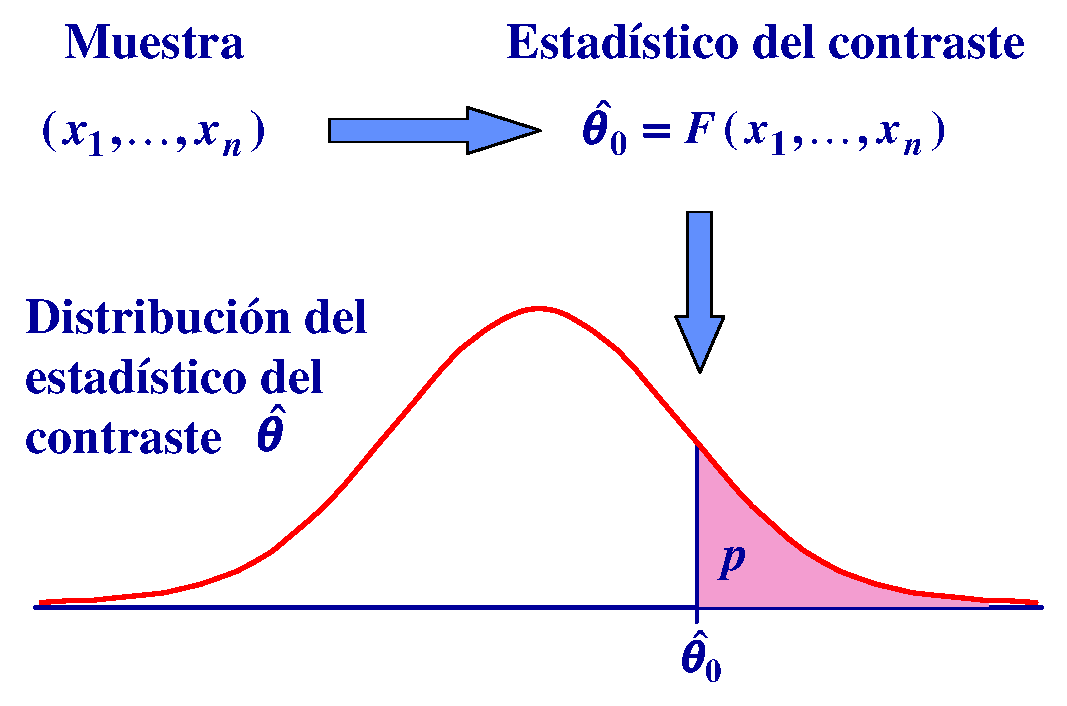
\includegraphics[scale=0.5]{contrastes/img/estadisticocontraste}
\caption{El $p$-valor de un contraste unilateral con cola a la derecha.}
\label{g:pvalor}
\end{center}
\end{figure}

Una vez calculado el $p$-valor, si hemos fijado el nivel de significación $\alpha$ y han quedado delimitadas las
regiones de aceptación y rechazo, el que la estimación caiga dentro de la región de rechazo es equivalente a que
$p<\alpha$, mientras que si cae dentro de la región de aceptación, entonces $p\geq \alpha$.
Esta forma de abordar los contrastes, nos da una visión más amplia, ya que nos da información de para qué niveles de
significación puede rechazarse la hipótesis nula, y para cuales no se puede.


\subsubsection{Contrastes y Estadísticos de Contraste}
Apoyándose en las distintas distribuciones en el muestreo comentadas en las prácticas sobre intervalos de confianza, a
continuación se presentan las fórmulas para los principales estadísticos de contraste.

\subsubsection{Contraste para la media de una población normal con varianza conocida}
\begin{itemize}
\item Hipótesis Nula: $H_0:\ \mu=\mu_0$
\item Estadístico del contraste:
\[
\dfrac{\overline{X}-\mu_0 }{\dfrac{\sigma }{\sqrt{n}}}
\]
que sigue una distribución normal tipificada, $N(0,1)$.
\end{itemize}
Este contraste también es válido para la media de una población no normal, siempre y cuando las muestras sean grandes
$(n\geq 30)$, con varianza conocida; y para la media de la diferencia de datos emparejados, siempre y cuando la variable
diferencia siga una distribución normal con varianza conocida, o una distribución cualquiera si la muestra es grande.

\subsubsection{Contraste para la media de una población normal con varianza desconocida}
\begin{itemize}
\item Hipótesis Nula: $H_0:\ \mu=\mu_0$
\item Estadístico del contraste:
\[
\dfrac{\overline{X}-\mu_0}{\dfrac{S_{n-1}}{\sqrt{n}}}
\]
que sigue una distribución $t$ de Student con $n-1$ grados de libertad, $T(n-1)$.
\end{itemize}
Este contraste también es válido para la media de una población no normal en muestras grandes $(n\geq 30)$, con varianza
desconocida; y para la media de la diferencia de datos emparejados, siempre y cuando la variable diferencia siga una
distribución normal con varianza desconocida, o una distribución cualquiera si la muestra es grande.

\subsubsection{Contraste para la proporción en muestras grandes y distribuciones simétricas (tanto $np$ como $n(1-p)$
deben ser mayores que 5)}
\begin{itemize}
\item Hipótesis Nula: $H_0:\ p=p_0$
\item Estadístico del contraste:
\[
\frac{{p - p_0 }}{{\sqrt {\frac{{p\left( {1 - p} \right)}}{n}} }}
\]
que sigue una distribución normal tipificada, $N(0,1)$.
\end{itemize}


\subsubsection{Contraste para la varianza de una población normal}
\begin{itemize}
\item Hipótesis Nula: $H_0:\ \sigma^2=\sigma_0^2$
\item Estadístico del contraste:
\[
\frac{{\left( {n - 1} \right)S_{n - 1} ^2 }}{{\sigma _0 ^2 }}
\]
que sigue una distribución Chi-cuadrado con $n-1$ grados de libertad.
\end{itemize}

\subsubsection{Contraste para la diferencia de medias de poblaciones normales con varianzas conocidas}
\begin{itemize}
\item Hipótesis Nula: $H_0:\ \mu_1=\mu_2$
\item Estadístico del contraste:
\[
\frac{{\overline X  - \overline Y }}{{\sqrt {\frac{{\sigma _1 ^2}}{{n_1 }} + \frac{{\sigma _2 ^2 }}{{n_2 }}} }}
\]
que sigue una distribución normal tipificada, $N(0,1)$.
\end{itemize}
Este contraste también es válido para la diferencia de medias de dos poblaciones no normales, siempre y cuando las
muestras sean grandes ($n_1\geq 30$ y $n_2\geq 30$), con varianzas conocidas.

\subsubsection{Contraste para la diferencia de medias de poblaciones normales con varianzas desconocidas}
\begin{itemize}
\item Hipótesis Nula: $H_0:\ \mu_1=\mu_2$
\item Estadístico del contraste:
\[
\frac{{\overline X  - \overline Y }}{{\sqrt {\frac{{S_{1,n_1-1} ^2}}{{n_1 }} + \frac{{S_{2,n_2-1} ^2 }}{{n_2 }}} }}
\]
que sigue una distribución t de Student con $\nu$ grados de libertad, donde $\nu$ es el número entero más próximo al
valor de la expresión:
\[
\dfrac{\left( \dfrac{s_{1,n_{1}-1}^{2}}{n_{1}}+\dfrac{s_{2,n_{2}-1}^{2}}{n_{2}}\right)
^{2}}{\dfrac{\left(\dfrac{s_{1,n_{1}-1}^{2}}{n_{1}}\right)^{2}}{n_{1}+1}+\dfrac{\left(
\dfrac{s_{2,n_{2}-1}^{2}}{n_{2}}\right) ^{2}}{n_{2}+1}}-2.
\]
\end{itemize}
Este contraste también es válido para la diferencia de medias de dos poblaciones no normales, siempre y cuando las
muestras sean grandes ($n_1\geq 30$ y $n_2\geq 30$), con varianzas desconocidas.

\subsubsection{Contraste para la diferencia de proporciones en muestras grandes y distribuciones simétricas ($n_1p_1$, $n_1(1-p_1)$, $n_2p_2$,
$n_2(1-p_2)$ deben ser mayores que 5)}
\begin{itemize}
\item Hipótesis Nula: $H_0:\ p_1=p_2$
\item Estadístico del contraste:
\[
\frac{{p_1  - p_2 }}{{\sqrt {\frac{{p_1 \left( {1 - p_1 }\right)}}{{n_1 }} + \frac{{p_2 \left( {1 - p_2 } \right)}}{{n_2}}} }}
\]
que sigue una distribución normal tipificada, $N(0,1)$.
\end{itemize}

\subsubsection{Contraste para la igualdad de varianzas de poblaciones normales}
\begin{itemize}
\item Hipótesis Nula: $H_0:\ \sigma_1^2=\sigma_2^2$
\item Estadístico del contraste:
\[
\frac{{S^2 _{1,n_1  - 1} }}{{S^2 _{2,n_2  - 1} }}
\]
que sigue una distribución F de Fisher con $n_1-1$ y $n_2-1$ grados de libertad.
\end{itemize}

\clearpage
\newpage

\section{Ejercicios resueltos}
\begin{enumerate}[leftmargin=*]
\item Para averiguar si en una determinada población existen menos hombres que mujeres se plantea un contraste de
hipótesis sobre la proporción de hombres que hay en la población: $H_0:\ p=0.5$ frente a $H_1:\ p<0.5$ y para ello se
toma una muestra aleatoria de 10 personas. 
Se pide:
\begin{enumerate}
\item Suponiendo cierta la hipótesis nula, ¿qué distribución sigue la variable que mide el número de hombres en la
muestra de tamaño 10?
\item Suponiendo cierta la hipótesis nula, ¿cuál es la probabilidad de que en la muestra se obtengan 0 hombres?
¿Se aceptaría la hipótesis nula en tal caso? 
Justificar la respuesta.
\begin{indicacion}{
\begin{enumerate}
\item Seleccionar el menú \menu{Teaching\flecha Distribuciones\flecha Discretas\flecha Binomial\flecha
Probabilidades acumuladas}.
\item En el cuadro de diálogo que aparece, introducir 0 en el campo \campo{Valor(es) de la variable}, 10 en el campo
\campo{Nº de repeticiones}, $0.5$ en el campo \campo{Probabilidad de éxito}, marcar la opción \opcion{Cola izquierda} y
hacer click en el botón \boton{Aceptar}.
\end{enumerate}}
\end{indicacion}

\item Suponiendo cierta la hipótesis nula, si se decide rechazarla cuando en la muestra haya 2 o menos hombres, ¿cuál es
el riesgo de equivocarse?
\begin{indicacion}{
\begin{enumerate}
\item Seleccionar el menú \menu{Teaching\flecha Distribuciones\flecha Discretas\flecha Binomial\flecha
Probabilidades acumuladas}.
\item En el cuadro de diálogo que aparece, introducir 2 en el campo \campo{Valor(es) de la variable}, 10 en el campo
\campo{Nº de repeticiones}, $0.5$ en el campo \campo{Probabilidad de éxito}, marcar la opción \opcion{Cola izquierda} y
hacer click en el botón \boton{Aceptar}.
\end{enumerate}}
\end{indicacion}

\item Si el máximo riesgo de error $\alpha$ que se tolera es $0.05$, ¿qué número de hombres en la muestra formarían la
región de rechazo de la hipótesis nula?
\begin{indicacion}{
\begin{enumerate}
\item Seleccionar el menú \menu{Teaching\flecha Distribuciones\flecha Discretas\flecha Binomial\flecha
Probabilidades acumuladas}.
\item En el cuadro de diálogo que aparece, introducir 1 en el campo \campo{Valor(es) de la variable}, 10 en el campo
\campo{Nº de repeticiones}, $0.5$ en el campo \campo{Probabilidad de éxito}, marcar la opción \opcion{Cola izquierda} y
hacer click en el botón \boton{Aceptar}.
\end{enumerate}}
\end{indicacion}

\item Suponiendo que la proporción real de hombres en la población fuese de $0.4$, ¿cuál es la potencia del contraste
para la región de rechazo del apartado anterior?
\begin{indicacion}{
\begin{enumerate}
\item Seleccionar el menú \menu{Teaching\flecha Distribuciones\flecha Discretas\flecha Binomial\flecha
Probabilidades acumuladas}.
\item En el cuadro de diálogo que aparece, introducir 1 en el campo \campo{Valor(es) de la variable}, 10 en el campo
\campo{Nº de repeticiones}, $0.4$ en el campo \campo{Probabilidad de éxito}, marcar la opción \opcion{Cola izquierda} y
hacer click en el botón \boton{Aceptar}.
\end{enumerate}}
\end{indicacion}

\item Si en lugar de una muestra de tamaño 10 se tomase una muestra de tamaño 100, y haciendo uso de la aproximación de
una distribución binomial mediante una normal, ¿qué número de hombres en la muestra formarían la región de rechazo para
un riesgo $\alpha=0.05$? 
¿Qué potencia tendría ahora el contraste si la proporción real de hombres fuese de $0.4$? 
¿Es mejor o peor contraste que el anterior? 
Justificar la respuesta.
\begin{indicacion}{
Una distribución binomial $B(100,\, 0.5)$ puede aproximarse mediante una normal $N(50,5)$.
\begin{enumerate}
\item Seleccionar el menú \menu{Teaching\flecha Distribuciones\flecha Continuas\flecha Normal\flecha
Cuantiles}.
\item En el cuadro de diálogo que aparece, introducir las probabilidad $0.05$ en el campo \campo{Probabilidades}, 50 en
el campo \campo{media}, 5 en el campo \campo{desviación típica}, marcar la opción \opcion{Cola izquierda} y hacer click
en el botón \boton{Aceptar}.
\end{enumerate}
El valor obtenido es la frontera entre la región de aceptación y la región de rechazo. 
Si en la muestra se obtienen menos hombres de dicho valor se rechazará la hipótesis nula, mientras que si se obtienen
más se aceptará. 
Para calcular la potencia de contraste:
\begin{enumerate}
\item Seleccionar el menú \menu{Teaching\flecha Distribuciones\flecha Continuas\flecha Normal\flecha
Probabilidades acumuladas}.
\item En el cuadro de diálogo que aparece, introducir el valor de la frontera en el campo \campo{Valor(es) de la
variable}, 40 en el campo \campo{media}, $4.899$ en el campo \campo{desviación típica}, marcar la opción \opcion{Cola
izquierda} y hacer click en el botón \boton{Aceptar}.
\end{enumerate}}
\end{indicacion}

\item Si se toma una muestra de tamaño 100 y se observan 41 hombres, ¿cuál es $p$-valor del contraste? 
¿Podría rechazarse la hipótesis nula pra un riesgo $\alpha=0.05$? 
¿y para un riesgo $\alpha=0.01$?
\begin{indicacion}{
\begin{enumerate}
\item Seleccionar el menú \menu{Teaching\flecha Test paramétricos\flecha Proporciones\flecha Test para una proporción}.
\item En el cuadro de diálogo que aparece marcar la casilla de \opcion{Introducción manual de frecuencias}, introducir
41 en el campo \campo{Frecuencia muestral} e introducir 100 en el campo \campo{Tamaño muestral}.
\item En la solapa \menu{Opciones de contraste}, introducir $0.5$ en el campo \campo{Hipótesis nula}, seleccionar
como hipótesis alternativa \opcion{Unilateral menor} y hacer click en el botón \boton{Aceptar}.
\end{enumerate}}
\end{indicacion}
\end{enumerate}


\item  Se analiza la concentración de principio activo en una muestra de 10 envases tomados de un lote de un fármaco, obteniendo los
siguientes resultados en mg/mm$^{3}$: 
\[ 
17.6-19.2-21.3-15.1-17.6-18.9-16.2-18.3-19.0-16.4 
\]
Se pide:
\begin{enumerate}
\item Crear un conjunto de datos con la variable \variable{concentracion}.

\item Realizar el contraste de hipótesis bilateral: $H_0$: $\mu=18$ y $H_1$: $\mu\neq18$ con un nivel de significación
$0.05$.
\begin{indicacion}{
\begin{enumerate}
\item Seleccionar el menú \menu{Teaching\flecha Test paramétricos\flecha Medias\flecha Test t para una muestra}.
\item En el cuadro de diálogo que aparece seleccionar la variable \variable{concentracion}.
\item En la solapa \menu{Opciones de contraste}, introducir 18 en el campo \campo{Hipótesis nula}, seleccionar como
hipótesis alternativa la opción \opcion{Bilateral} y hacer click sobre el botón \boton{Aceptar}.
\end{enumerate}}
\end{indicacion}

\item De igual manera realizar los contrastes bilaterales: $H_0$: $\mu=19.5$ y $H_1$: $\mu\neq19.5$ con un niveles de
significación $0.05$ y $0.01$.
¿Cómo afecta la disminución en el nivel de significación en la facilidad para rechazar $H_0$?

\begin{indicacion}{Seguir los mismos pasos del apartado anterior introduciendo $19.5$ en el campo \campo{Hipótesis nula}.}
\end{indicacion}

\item Realizar los contrastes bilaterales y unilaterales para la hipótesis nula $H_0$: $\mu=17$ con un nivel de significación de $0.05$.
¿Qué relación hay entre el $p$-valor de los contrastes bilateral y unilaterales?
\begin{indicacion}{
\begin{enumerate}
\item Seleccionar el menú \menu{Teaching\flecha Test paramétricos\flecha Medias\flecha Test t para una muestra}.
\item En el cuadro de diálogo que aparece seleccionar la variable \variable{concentracion}.
\item En la solapa \menu{Opciones de contraste}, introducir 17 en el campo \campo{Hipótesis nula}, seleccionar como
hipótesis alternativa \opcion{Bilateral} y hacer click sobre el botón \boton{Aceptar}.
\item Para el contraste de menor repetir lo mismo seleccionando como hipótesis alternativa \opcion{Unilateral menor}.
\item Para el contraste de mayor repetir lo mismo seleccionando como hipótesis alternativa \opcion{Unilateral mayor}.
\end{enumerate}
}
\end{indicacion}

\item Si el fabricante del lote asegura haber aumentado la concentración de principio activo con respecto a anteriores
lotes, en los que la media era de 17 mg/mm$^3$, ¿se acepta o se rechaza la afirmación del fabricante?

\item ¿Cuál sería el tamaño muestral requerido para poder detectar una diferencia de $0.5$ mg/mm$^{3}$ más con un nivel de
significación $\alpha=0.05$ y una potencia $1-\beta=0.8$?
\begin{indicacion}{
Para calcular el tamaño muestral se necesita saber la desviación típica de la población o una estimación suya. 
Para ello se calcula previamente la cuasivarianza muestral
\begin{enumerate}
\item Seleccionar el menú \menu{Teaching\flecha Estadística descriptiva\flecha Estadísticos}.
\item En el cuadro de diálogo que aparece seleccionar la variable \variable{concentracion}.
\item En la solapa \menu{Estadísticos básicos} marcar la opción \opcion{Cuasidesviación típica} y hacer click en el
botón \boton{Aceptar}.
\end{enumerate}
Para calcular el tamaño muestral:
\begin{enumerate}
\item Seleccionar el menú \menu{Teaching\flecha Test paramétricos\flecha Medias\flecha Cálculo del tamaño muestral para el test T}.
\item En el cuadro de diálogo que aparece introducir en el campo \campo{Diferencia en las medias} el valor 0.5,
introducir en el campo \campo{Desviación típica} el valor de la cuasivesviación típica obtenido, introducir el valor
$0.05$ en el campo \campo{Nivel de significación}, introducir el valor $0.8$ en el campo \campo{Potencia}, marcar la
opción \opcion{Una muestra} en el campo \campo{Tipo de test}, seleccionar como hipótesis alternativa \opcion{Unilateral}
y hacer click sobre el botón \boton{Aceptar}.
\end{enumerate}
}
\end{indicacion}
\end{enumerate}


\item En una encuesta realizada en una facultad, sobre si el alumnado utiliza habitualmente (al menos una vez a la
semana) la biblioteca de la misma, se han obtenido los siguientes resultados:
\begin{flushleft}
\begin{tabular}{|l|l|l|l|l|l|l|l|l|l|l|l|l|l|l|l|l|l|}
\hline
Alumno & 1 & 2 & 3 & 4 & 5 & 6 & 7 & 8 & 9 & 10 & 11 & 12 & 13 & 14 & 15 & 16 & 17 \\
\hline
Respuesta & no & si & no & no & no & si & no & si & si & si & si & no & si & no & si & no & no \\
\hline
\end{tabular}
\newline

\begin{tabular}{|l|l|l|l|l|l|l|l|l|l|l|l|l|l|l|l|l|l|}
\hline
Alumno & 18 & 19 & 20 & 21 & 22 & 23 & 24 & 25 & 26 & 27 & 28 & 29 & 30 & 31 & 32 & 33 & 34 \\
\hline
Respuesta & no & si & si & si & no & no & si & no & no & si & si & no & no & si & no & si & no \\
\hline
\end{tabular}
\end{flushleft}

\begin{enumerate}
\item Crear un conjunto de datos con la variable \variable{respuesta} como factor.

\item Contrastar si el porcentaje de alumnos que utiliza regularmente la biblioteca es superior al 40\%. 
\begin{indicacion}{
\begin{enumerate}
\item Seleccionar el menú \menu{Teaching\flecha Test paramétricos\flecha Proporciones\flecha Test para una proporción}.
\item En el cuadro de diálogo que aparece seleccionar la variable \variable{respuesta} e introducir \texttt{Si} en el campo \campo{Categoría}.
\item En la solapa \menu{Opciones de contraste}, introducir $0.4$ en el campo \campo{Hipótesis nula}, seleccionar como
hipótesis alternativa \opcion{Unilateral mayor} y hacer click en el botón \boton{Aceptar}.
\end{enumerate}
}
\end{indicacion}
\end{enumerate}

\item Varios investigadores desean saber si es posible concluir que dos poblaciones de niños difieren respecto a la edad
promedio en la cual pueden caminar por sí solos.
Los investigadores obtuvieron los siguientes datos para la edad al comenzar a andar (expresada en meses):
\begin{center}
\begin{tabular}{ll}
Muestra en la población $A$: & $9.5-10.5-9.0-9.8-10.0-13.0-10.0-13.5-10.0-9.8$\\
Muestra en la población $B$: & $12.5-9.5-13.5-13.8-12.0-13.8-12.5-9.5-12.0-13.5-12.0-12.0$
\end{tabular}
\end{center}

\begin{enumerate}
\item Crear un conjunto de datos con las variables \variable{población} y \variable{edad}.

\item Realizar un contraste de hipótesis con un nivel de significación de $0.05$ para dar respuesta a la conclusión que
buscan los investigadores.
\begin{indicacion}{
Primero hay que realizar un constraste de comparación de varianzas.
\begin{enumerate}
\item Seleccionar el menú \menu{Teaching\flecha Test paramétricos\flecha Varianzas\flecha Test F para dos varianzas}.
\item En el cuadro de dialogo que aparece seleccionar la variable \variable{edad} en el campo \campo{Comparar} y la
variable \variable{población} en el campo \campo{Según}.
\item En la solapa \menu{Opciones de contraste} seleccionar como hipótesis alternativa \opcion{Bilateral} y hacer click
sobre el botón \boton{Aceptar}.
\end{enumerate}
Se mantiene la hipótesis de igualdad de varianzas con la confianza fijada si el el $p$-valor es mayor que $0.5$. 
Después se realiza el contraste de comparación de medias.
\begin{enumerate}
\item Seleccionar el menú \menu{Teaching\flecha Test paramétricos\flecha Medias\flecha Test t para dos muestras independientes}.
\item En el cuadro de dialogo que aparece seleccionar la variable \variable{edad} en el campo \campo{Comparar} y la
variable \variable{población} en el campo \campo{Según}.
\item En la solapa \menu{Opciones de contraste} seleccionar como hipótesis alternativa \opcion{Bilateral},
marcar la casilla \opcion{Suponer varianzas iguales} y hacer click sobre el botón \boton{Aceptar}.
\end{enumerate}
Hay diferencias entre las poblaciones si el $p$-valor es menor que $0.05$.
}
\end{indicacion}
\end{enumerate}


\item Algunos investigadores han observado una mayor resistencia de las vías respiratorias en fumadores que en no
fumadores.
Para confirmar dicha hipótesis, se realizó un estudio para comparar el porcentaje de retención traqueobronquial en las
mismas personas cuando aún eran fumadoras y transcurrido un año después de dejarlo.
Los resultados se indican en la tabla siguiente:
\[
\begin{array}{cc}
\hline
\multicolumn{2}{c}{\text{Porcentaje de retención}} \\
\hline
\text{Cuando fumaba} & \text{Transcurrido un año sin fumar} \\
\hline
60.6 & 47.5 \\
12.0 & 13.3 \\
56.0 & 33.0 \\
75.2 & 55.2 \\
12.5 & 21.9 \\
29.7 & 27.9 \\
57.2 & 54.3 \\
62.7 & 13.9 \\
28.7 & 8.90 \\
66.0 & 46.1 \\
25.2 & 29.8 \\
40.1 & 36.2 \\
\hline
\end{array}
\]

\begin{enumerate}
\item Crear un conjunto de datos con las variables \variable{antes} y \variable{después} e introducir los datos.

\item Plantear el contraste de hipótesis adecuado para confirmar o denegar la hipótesis de los investigadores. 
\begin{indicacion}{
\begin{enumerate}
\item Seleccionar el menú \menu{Teaching\flecha Test paramétricos\flecha Medias\flecha Test t para dos muestras pareadas}.
\item En el cuadro de diálogo que aparece seleccionar la variable \variable{antes} en el campo \campo{Comparar} y la variable
\variable{después} en el campo \campo{Con}.
\item En la solapa \menu{Opciones de contraste} seleccionar como hipótesis alternativa \opcion{Unilateral mayor} y hacer
click en el botón \boton{Aceptar}.
\end{enumerate}
}
\end{indicacion}
\end{enumerate}


\item Un profesor universitario ha tenido dos grupos de clase a lo largo del año: uno con horario de mañana y otro de
tarde. En el de mañana, sobre un total de 80 alumnos, han aprobado 55; y en el de tarde, sobre un total de 90 alumnos,
han aprobado 32. 
¿Se puede afirmar que hay diferencias significativas entre los porcentajes de aprobados en ambos grupos? 
Justificar la respuesta.
\begin{enumerate}
\begin{indicacion}{
\begin{enumerate}
\item Seleccionar el menú \menu{Teaching\flecha Test paramétricos\flecha Proporciones\flecha Test para dos proporciones}, marcar la casilla \opcion{Introducción manual de frecuencias}, introducir 55 en el campo \campo{Frecuencia muestral 1}, introducir 80 en el campo
\campo{Tamaño muestral 1}, introducir 32 en el campo \campo{Frecuencia muestral 2} e introducir 90 en el campo
\campo{Tamaño muestral 2}.
\item En la solapa \menu{Opciones de contraste}, seleccionar como hipótesis alternativa \opcion{Bilateral} y hacer click
en el botón \boton{Aceptar}.
\end{enumerate}}
\end{indicacion}
\end{enumerate}

\end{enumerate}


\section{Ejercicios propuestos}
\begin{enumerate}[leftmargin=*] 
\item El fichero \texttt{pulso.txt} contiene información sobre el pulso de un grupo de pacientes que han realizado
distintos ejercicios:
pulso en reposo (pulse1), pulso después de hacer ejercicio (pulse2), tipo de ejercicio (ran, 1=correr, 2=andar), sexo
(sex, 1=hombre, 2=mujer) y peso (weight).
Se pide:
\begin{enumerate}
\item Contrastar si el pulso en reposo está por debajo de 75 pulsaciones.
\item ¿Qué tamaño muestral sería necesario para detectar una diferencia de 2 pulsaciones más en la media de las
pulsaciones en reposo, con un nivel de significación $0.05$ y una potencia de $0.9$?
\item Contrastar si el pulso después de correr está por encima de 85 pulsaciones.
\item Contrastar si el porcentaje de personas con taquicardia leve (número de pulsaciones en reposo por encima de 90)
supera el 5\%.
\item ¿Se puede afirmar que el ejercicio aumenta las pulsaciones con una significación de $0.05$? 
¿y con una significación $0.01$?
Justificar la respuesta.
\item ¿Existen diferencias entre las pulsaciones después de andar y después de correr? Justificar la respuesta.
\item ¿Existen diferencias entre las pulsaciones en reposo entre hombres y mujeres? 
¿Y entre las pulsaciones después de correr? Justificar la respuesta.
\end{enumerate}

\end {enumerate}

% Version control information:
%$HeadURL: https://practicas-r.googlecode.com/svn/trunk/anova_1_factor/anova_1_factor.tex $
%$LastChangedDate: 2011-12-05 14:06:12 +0100 (lun 05 de dic de 2011) $
%$LastChangedRevision: 19 $
%$LastChangedBy: asalber $
%$Id: anova_1_factor.tex 19 2011-12-05 13:06:12Z asalber $

\chapter{Análisis de la Varianza de 1 Factor}

\section{Fundamentos teóricos}

El \emph{Análisis de la Varianza con un Factor} es una técnica
estadística de contraste de hipótesis, cuyo propósito es estudiar
el efecto de la aplicación de varios \emph{niveles}, también
llamados \emph{tratamientos}, de una variable aleatoria
cualitativa, llamada \emph{factor}, en una variable cuantitativa,
llamada \emph{respuesta}.

Por ejemplo, supongamos que estamos interesados en conocer si el sueldo medio de los médicos que entran a formar parte
de la plantilla de un hospital, depende de la comunidad autónoma en la que trabajan.
En este problema, la variable factor es la comunidad autónoma, con sus distintos niveles que son las distintas
comunidades, mientras que la variable respuesta es el sueldo cobrado.
A diferencia de un análisis de regresión simple, en el que se intenta explicar la variable respuesta mediante otra
variable cuantitativa (como por ejemplo, el sueldo en función de las horas de permanencia en el hospital, o de la
antigüedad en el puesto de trabajo), en el análisis de la varianza el factor, que es la variable independiente, es una
variable cualitativa.

Por otro lado, el análisis de la varianza de 1 factor se parece a un contraste de comparación de medias, sólo que en
dicho contraste se comparan las medias de dos poblaciones, mientras que en el análisis de la varianza se comparan las
medias de las $k$ poblaciones correspondientes a los $k$ niveles del factor.

Para comparar las medias de la variable respuesta según los diferentes niveles del factor, se realiza un contraste de
hipótesis en el que la hipótesis nula, $H_0$, es que la variable respuesta tiene igual media en todos los niveles,
mientras que la hipótesis alternativa, $H_1$, es que hay diferencias estadísticamente significativas en al menos dos de
las medias; y dicho contraste de hipótesis se basa en la comparación de dos estimadores de la varianza total de los
datos de la variable respuesta; de ahí procede el nombre de esta técnica: \emph{ANOVA} (Analysis of Variance).

\subsection{Notación, Modelo y Contraste}
La notación habitual en ANOVA es la siguiente:
\begin{description}
\item[$k$] es el número de niveles del factor.
\item[$n_i$] es el tamaño de la muestra aleatoria correspondiente al nivel $i$-ésimo del factor.
\item[$n = \sum_{i = 1}^k {n_i}$] es el número total de observaciones.
\item[$X_{ij}\ (i = 1,...,k;\,j = 1,...,n_i)$] es una variable aleatoria que indica la respuesta de la $j$-ésima unidad
experimental al $i$-ésimo nivel del factor.
\item [$x_{ij}$] es el valor concreto, en una muestra dada, de la variable $X_{ij}$.

\begin{center}
\begin{tabular}{|l|l|l|l|}
\hline
\multicolumn{4}{|c|}{Nivel del Factor} \\
\hline
\multicolumn{1}{|c|}{$1$} & \multicolumn{1}{c|}{$2$} & \multicolumn{1}{c|}{$\cdots$} & \multicolumn{1}{c|}{$k$} \\
\hline
\multicolumn{1}{|c|}{$X_{11}$} & \multicolumn{1}{c|}{$X_{21}$} & \multicolumn{1}{c|}{$\cdots$} &
\multicolumn{1}{c|}{$X_{k1}$}
\\
\hline
\multicolumn{1}{|c|}{$X_{12}$} & \multicolumn{1}{c|}{$X_{22}$} & \multicolumn{1}{c|}{$\cdots$} & \multicolumn{1}{c|}{$X_{k2}$} \\
\hline
\multicolumn{1}{|c|}{$\cdots$} & \multicolumn{1}{c|}{$\cdots$} & \multicolumn{1}{c|}{$\cdots$} & \multicolumn{1}{c|}{$\cdots$} \\
\hline
\multicolumn{1}{|c|}{$X_{1n_1}$} & \multicolumn{1}{c|}{$X_{2n_2}$} & \multicolumn{1}{c|}{$\cdots$} &
\multicolumn{1}{c|}{$X_{kn_k}$}
\\
\hline
\multicolumn{1}{c|}{} & \multicolumn{1}{c|}{$X_{2n_2}$} & \multicolumn{1}{c}{} & \multicolumn{1}{c}{} \\
\cline{2-2}
\end {tabular}
\end{center}

\item[$\mu_i$] es la media de la población del nivel $i$.
\item [$\overline X_i = \sum_{j = 1}^{n_i} X_{ij}/n_i$] es la variable media muestral del nivel $i$, y
estimador de $\mu_i$.
\item [$\overline x_i = \sum_{j = 1}^{n_i} x_{ij}/n_i$] es la estimación concreta para una muestra dada de la
variable media muestral del nivel $i$.
\item [$\mu$] es la media de la población incluidos todos los niveles.
\item [$\overline X  = \sum_{i = 1}^k \overline X_i/k = \sum_{i = 1}^k \sum_{j = 1}^{n_i } X_{ij}/n$] es la variable
media muestral de todas las respuestas, y estimador de $\mu$.
\item [$\overline x  = \sum_{i = 1}^k \overline x_i/k = \sum_{i = 1}^k \sum_{j = 1}^{n_i } x_{ij}/n$] es la estimación
concreta para una muestra dada de la variable media muestral.
\end{description}

Con esta notación podemos expresar la variable respuesta mediante un modelo matemático que la descompone en componentes
atribuibles a distintas causas:
\[
X_{ij}  = \mu  + \left( {\mu _i  - \mu } \right) + \left(
{X_{ij} - \mu _i } \right),
\]
es decir, la respuesta $j$-ésima en el nivel $i$-ésimo puede descomponerse como resultado de una media global, más la
desviación con respecto a la media global debida al hecho de que recibe el tratamiento $i$-ésimo, más una nueva
desviación con respecto a la media del nivel debida a influencias aleatorias.

Sobre este modelo se plantea la hipótesis nula: las medias correspondientes a todos los niveles son iguales; y su
correspondiente alternativa: al menos hay dos medias de nivel que son diferentes.
\[
\begin{cases}
H_0 &: & \mu _1  = \mu _2  = ... = \mu _k\\
H_1 &: & \mu _i  \neq  \mu _j \;\textrm{para algún}\, i\,\textrm{y}\, j
\]

Para poder realizar el contraste con este modelo es necesario plantear ciertas hipótesis estructurales (supuestos del
modelo):

\begin{itemize}
\item Las $k$ muestras, correspondientes a los $k$ niveles del factor, representan muestras aleatorias independientes de
$k$ poblaciones con medias $\mu _1  = \mu _2  = ... = \mu _k$ desconocidas.
\item Cada una de las $k$ poblaciones es normal.
\item Cada una de las $k$ poblaciones tiene la misma varianza, $\sigma^2$.
\end{itemize}

Teniendo en cuenta la hipótesis nula y los supuestos del modelo, podemos construir un estadístico del contraste con
distribución conocida, tal que permite aceptar o rechazar $H_0$; pero hasta poder dar el valor de dicho estadístico, aún
debemos seguir ampliando la notación habitual en los test de ANOVA.

Si sustituimos en el modelo las medias poblacionales por sus correspondientes estimadores muestrales tenemos
\[
X_{ij}  = \overline X  + \left( {\overline X_i  - \overline X }
\right) + \left( {X_{ij}  - \overline X_i } \right),
\]
o lo que es lo mismo,
\[
X_{ij}- \overline X =   \left( {\overline X_i  - \overline X }
\right) + \left( {X_{ij}  - \overline X_i } \right).
\]

Elevando al cuadrado y teniendo en cuenta las propiedades de los sumatorios, se llega a la ecuación que recibe el nombre
de \emph{identidad de la suma de cuadrados}:
\[
\sum\limits_{i = 1}^k {\sum\limits_{j = 1}^{n_i } {\left( {X_{ij}
- \overline X } \right)^2 } }  = \sum\limits_{i = 1}^k {n_i\left(
{\overline X_i  - \overline X } \right)^2 }  + \sum\limits_{i =
1}^k {\sum\limits_{j = 1}^{n_i } {\left( {X_{ij}  - \overline X_i
} \right)^2 } },
\]
donde:
\begin{description}
\item [$\sum_{i = 1}^k \sum_{j = 1}^{n_i } (X_{ij}- \overline X )^2$] recibe el nombre de \emph{suma total de
cuadrados}, ($STC$), y es la suma de cuadrados de las desviaciones con respecto a la media global; por lo tanto, una
medida de la variabilidad total de los datos.
\item [$\sum_{j = 1}^k n_i (\overline X_i  - \overline X)^2$] recibe el nombre de \emph{suma de cuadrados de los
tratamientos o suma de cuadrados intergrupos}, ($SCInter$), y es la suma ponderada de cuadrados de las desviaciones de
la media de cada nivel con respecto a la media global; por lo tanto, una medida de la variabilidad atribuida al hecho de
que se utilizan diferentes niveles o tratamientos.
\item [$\sum_{i = 1}^k \sum_{j = 1}^{n_i } (X_{ij}- \overline X_i )^2$] recibe el nombre de \emph{suma de cuadrados
residual o suma de cuadrados intragrupos}, ($SCIntra$), y es la suma de cuadrados de las desviaciones de las
observaciones con respecto a las medias de los sus respectivos niveles o tratamientos; por lo tanto, una medida de la
variabilidad en los datos atribuida a las fluctuaciones aleatorias dentro del mismo nivel.
\end{description}

Con esta notación la identidad de suma de cuadrados se expresa:
\[
SCT=SCInter+SCIntra
\]
Y un último paso para llegar al estadístico que permitirá contrastar $H_0$, es la definición de los \emph{Cuadrados
Medios}, que se obtienen al dividir cada una de las sumas de cuadrados por sus correspondientes grados de libertad.
Para $SCT$ el número de grados de libertad es $n-1$; para $SCInter$ es $k-1$; y para $SCIntra$ es $n-k$.
Por lo tanto,
\begin{align*}
CMT &= \frac{{SCT}}{{n - 1}}\\
CMInter &= \frac{{SCInter}}{{k - 1}}\\
CMIntra &= \frac{{SCIntra}}{{n -k}}
\end{align*}

Y se podría demostrar que, en el supuesto de ser cierta la hipótesis nula y los supuestos del modelo, el cociente:
\[
\frac{{CMInter}}{{CMIntra}}
\] 
sigue una distribución $F$ de Fisher con $k-1$ y $n-k$ grados de libertad.

De forma que, si $H_0$ es cierta, el valor del cociente para un conjunto de muestras dado, estará próximo a 1 (aún
siendo siempre mayor que 1); pero si no se cumple $H_0$ crece la variabilidad intergrupos y la estimación del
estadístico crece.
En definitiva realizaremos un contraste de hipótesis unilateral con cola a la derecha de igualdad de varianzas, y para
ello calcularemos el $p$-valor de la estimación de $F$ obtenida y aceptaremos o rechazaremos en función del nivel de
significación fijado.

\subsubsection{Tabla de ANOVA}

Todos los estadísticos planteados en el punto anterior se recogen en una tabla denominada Tabla de ANOVA, en la que se
ponen los resultados de las estimaciones de dichos estadísticos en las muestras concretas objeto de estudio.
Esas tablas también son las que aportan como resultado de cualquier ANOVA los programas estadísticos, que suelen añadir
al final de la tabla el $p$-valor del $F$ calculado, y que permite aceptar o rechazar la hipótesis nula de que las
medias correspondientes a todos los niveles del factor son iguales.
\begin{center}
\renewcommand{\arraystretch}{2}
\begin{tabular}{|l|l|l|l|l|l|}
\cline{2-6}
\multicolumn{1}{c|}{} & \multicolumn{1}{p{1.5cm}|}{\centering Suma de \newline cuadrados} & \multicolumn{1}{p{1.8cm}|}{\centering Grados de\newline libertad} & \multicolumn{1}{p{3.5cm}|}{\centering\ \newline Cuadrados medios} & \multicolumn{1}{p{2.5cm}|}{\centering\ \newline Estadístico $F$} & \multicolumn{1}{p{1.5cm}|}{\centering\ \newline $p$-valor} \\

\hline
\multicolumn{1}{|l|}{Intergrupos} & \multicolumn{1}{c|}{$SCInter$} & \multicolumn{1}{c|}{$k-1$} & \multicolumn{1}{c|}{$CMInter = \dfrac{{SCInter}}{{k - 1}}$} & \multicolumn{1}{c|}{$f_0=\dfrac{{CMInter}}{{CMIntra}}$} & \multicolumn{1}{c|}{$P\left( {F > f_0} \right)$} \\
\hline
\multicolumn{1}{|l|}{Intragrupos} & \multicolumn{1}{c|}{$SCIntra$} & \multicolumn{1}{c|}{$n-k$} & \multicolumn{1}{c|}{$CMIntra = \dfrac{{SCIntra}}{{n -k}}$} & \multicolumn{1}{c|}{} & \multicolumn{1}{c|}{} \\
\hline
\multicolumn{1}{|l|}{Total} & \multicolumn{1}{c|}{$SCT$} & \multicolumn{1}{c|}{$n-1$} & \multicolumn{1}{c|}{} & \multicolumn{1}{c|}{} &  \\
\hline
\end{tabular}
\end{center}


\subsection*{Test de Comparaciones Múltiples y por Parejas} 
Una vez realizado el ANOVA de un factor para comparar las
$k$ medias correspondientes a los $k$ niveles o tratamientos del factor, nos encontramos en una de las dos siguientes
situaciones:
\begin{itemize}
\item No hemos podido rechazar $H_0$. En este caso se da por concluido el análisis de los datos en cuanto a detección de
diferencias entre los niveles.
\item Tenemos razones estadísticas para rechazar $H_0$. En este caso es natural continuar con el análisis para tratar de
localizar con precisión dónde está la diferencia, cuáles son el nivel o niveles cuyas respuestas son estadísticamente
diferentes.
\end{itemize}

En el segundo supuesto, hay varios métodos que permiten detectar las diferencias entre las medias de los diferentes
niveles, y que reciben el nombre de \emph{Test de Comparaciones Múltiples}.
A su vez este tipo de test se suelen clasificar en:
\begin{itemize}
\item \emph{Test de comparaciones por parejas}, cuyo objetivo es la comparación una a una de todas las posibles parejas
de medias que se pueden tomar al considerar los diferentes niveles.
Su resultado es una tabla en la que se reflejan las diferencias entre todas las posibles parejas y los intervalos de
confianza para dichas diferencias, con la indicación de si hay o no diferencias significativas entre las mismas.
Hay que aclarar que los intervalos obtenidos no son los mismos que resultarían si considerásemos cada pareja de medias
por separado, ya que el rechazo de $H_0$ en el contraste general de ANOVA implica la aceptación de una hipótesis
alternativa en la que están involucrados varios contrastes individuales a su vez; y si queremos mantener un nivel de
significación $\alpha$ en el general, en los individuales debemos utilizar un $\alpha '$ considerablemente más pequeño.
\item \emph{Test de rango múltiple}, cuyo objetivo es la identificación de subconjuntos homogéneos de medias que no se
diferencian entre sí.
\end{itemize}
Entre otros, para los primeros, el test de Bonferroni; para los segundos, el test de Duncan; y para ambas categorías a
la vez los test HSD de Tukey y Scheffé.

\clearpage
\newpage

\section{Ejercicios resueltos}
\begin {enumerate}[leftmargin=*]

\item Se realiza un estudio para comparar la eficacia de tres programas terapéuticos para el tratamiento del acné. Se
emplean tres métodos:
\begin{enumerate}
\item Lavado, dos veces al día, con cepillo de polietileno y un jabón abrasivo, junto con el uso diario de 250 mg de
tetraciclina.
\item Aplicación de crema de tretinoína, evitar el sol, lavado dos veces al día con un jabón emulsionante y agua, y
utilización dos veces al día de 250 mg de tetraciclina.
\item Evitar el agua, lavado dos veces al día con un limpiador sin lípidos y uso de crema de tretinoína y de peróxido
benzoílico.
\end{enumerate}
En el estudio participan 35 pacientes. Se separó aleatoriamente a estos pacientes en tres subgrupos de tamaños 10, 12 y
13, a los que se asignó respectivamente los tratamientos I, II, y III.
Después de 16 semanas se anotó para cada paciente el porcentaje de mejoría en el número de lesiones.
\[
\begin{array}{ll|ll|ll}
\multicolumn{6}{c}{\text{Tratamiento}} \\
\hline
\multicolumn{2}{c}{\text{I}} & \multicolumn{2}{c}{\text{II}} & \multicolumn{2}{c}{\text{III}} \\
\hline
48.6 & 50.8 & 68.0 & 71.9 & 67.5 & 61.4 \\
49.4 & 47.1 & 67.0 & 71.5 & 62.5 & 67.4 \\
50.1 & 52.5 & 70.1 & 69.9 & 64.2 & 65.4 \\
49.8 & 49.0 & 64.5 & 68.9 & 62.5 & 63.2 \\
50.6 & 46.7 & 68.0 & 67.8 & 63.9 & 61.2 \\
     &      & 68.3 & 68.9 & 64.8 & 60.5 \\
     &      &      &      & 62.3 &      \\
\hline
\end{array}
\]
\begin{enumerate}
\item Crear un conjunto de datos con las variables \variable{tratamiento} y \variable{mejora} e introducir los datos de
la muestra.

\item Dibujar el diagrama de puntos. ¿Se observan diferencias entre los tratamientos en el diagrama?
\begin{indicacion}{
\begin{enumerate}
\item Seleccionar el menú \menu{Teaching\flecha Gráficos\flecha Diagrama de puntos}.
\item En el cuadro de diálogo que aparece, seleccionar la variable \variable{mejora} en el campo \campo{Variable}, seleccionar la variable \variable{tratamiento} en el campo \campo{Grupos}, y hacer click sobre el botón
\boton{Aceptar}.
\end{enumerate}
}
\end{indicacion}

\item Realizar el contraste de ANOVA. 
¿Se puede concluir que los tres tratamientos tienen el mismo efecto medio con un nivel de significación de $0.05$?
\begin{indicacion}{
\begin{enumerate}
\item Seleccionar el menú \menu{Teaching\flecha Test paramétricos\flecha Medias\flecha ANOVA}.
\item En el cuadro de diálogo que aparece, seleccionar el conjunto de datos \variable{acne} en el campo \campo{Conjunto de datos}.
\item Seleccionar la variable \variable{mejora} en el campo \campo{Variable dependiente}, la variable
\variable{tratamiento} en el campo \campo{Factores entre individuos} y hacer click sobre el botón \boton{Aceptar}.
\end{enumerate}}
\end{indicacion}

\item Obtener la tabla de ANOVA correspondiente al problema pero que además muestre los intervalos de confianza de
comparación de los tres tratamientos con una significación de $0.05$.
¿Entre qué parejas de tratamientos hay diferencias estadísticamente significativas?
\begin{indicacion}{ 
Repetir los mismos pasos del apartado anterior activando la opción \opcion{Comparaciones de medias por pares} de la solapa \menu{Comparación por pares}.}
\end{indicacion}

\item Comprobar que se cumple la hipótesis de igualdad de varianzas entre los tratamientos.
\begin{indicacion}{ 
Repetir los mismos pasos del apartado anterior activando la opción \opcion{Test de Levene} de la solapa \menu{Opciones}.}
\end{indicacion}

\item Dibujar el gráfico de los intervalos de confianza para la media de cada tratamiento. 
\begin{indicacion}{
\begin{enumerate}
\item Seleccionar el menú \menu{Teaching \flecha Gráficos\flecha Diagrama de medias}.
\item En el cuadro de diálogo que aparece, seleccionar la variable \variable{mejora} en el campo \campo{Variable} y seleccionar la variable \variable{tratamiento} en el campo \campo{Grupos}.
\item Seleccionar la opción \opcion{Intervalos de confianza} y hacer click sobre el botón \boton{Aceptar}.
\end{enumerate}}
\end{indicacion}
\end{enumerate}


\item Se sospecha que hay diferencias en la preparación del examen de selectividad entre los diferentes centros de
bachillerato de una ciudad.
Con el fin de comprobarlo, de cada uno de los 5 centros, se eligieron 8 alumnos al azar, con la condición de que
hubieran cursado las mismas asignaturas, y se anotaron las notas que obtuvieron en el examen de selectividad. 
Los resultados fueron:
\[
\begin{array}{lllll}
\multicolumn{5}{c}{\text{Centros}} \\
\hline
1 & 2 & 3 & 4 & 5 \\
\hline
5.5 & 6.1 & 4.9 & 3.2 & 6.7 \\
5.2 & 7.2 & 5.5 & 3.3 & 5.8 \\
5.9 & 5.5 & 6.1 & 5.5 & 5.4 \\
7.1 & 6.7 & 6.1 & 5.7 & 5.5 \\
6.2 & 7.6 & 6.2 & 6.0 & 4.9 \\
5.9 & 5.9 & 6.4 & 6.1 & 6.2 \\
5.3 & 8.1 & 6.9 & 4.7 & 6.1 \\
6.2 & 8.3 & 4.5 & 5.1 & 7.0 \\
\hline
\end{array}
\]

\begin{enumerate}
\item Crear un conjunto de datos con las variables \variable{nota} y \variable{centro} e introducir los datos de la muestra.

\item Dibujar el diagrama de puntos. ¿Se observan diferencias entre los centros en el diagrama?
\begin{indicacion}{
\begin{enumerate}
\item Seleccionar el menú \menu{Teaching \flecha Gráficos\flecha Diagrama de puntos}.
\item En el cuadro de diálogo que aparece, seleccionar la variable \variable{nota} en el campo \campo{Variable}, seleccionar la
variable \variable{centro} en el campo \campo{Grupos} y hacer click sobre el botón \boton{Aceptar}.
\end{enumerate}
}
\end{indicacion}

\item Realizar el contraste de ANOVA. 
¿Se puede confimar la sospecha de que hay diferencias entre las notas medias de los centros?
\begin{indicacion}{
\begin{enumerate}
\item Seleccionar el menú \menu{Teaching\flecha Test paramétricos\flecha Medias\flecha ANOVA}.
\item En el cuadro de diálogo que aparece, seleccionar el conjunto de datos \variable{selectividad} en el campo \campo{Conjunto de datos}.
\item Seleccionar la variable \variable{notas} en el campo \campo{Variable dependiente}, la variable
\variable{centro} en el campo \campo{Factores entre individuos} y hacer click sobre el botón \boton{Aceptar}.
\end{enumerate}}
\end{indicacion}

\item ¿Qué centros son los mejores en la preparación de la selectividad?
\begin{indicacion}{ 
Repetir los mismos pasos del apartado anterior activando la opción \opcion{Comparaciones de medias por pares} de la solapa \menu{Comparación por pares}.}
\end{indicacion}
\end{enumerate}

\end{enumerate}


\section{Ejercicios propuestos}
\begin{enumerate}[leftmargin=*]

\item Se midió la frecuencia cardíaca (latidos por minuto) en cuatro grupos de adultos; controles normales (A),
pacientes con angina (B), individuos con arritmias cardíacas (C) y pacientes recuperados del infarto de miocardio (D).
Los resultados son los siguientes:

\begin{center}
\begin{tabular}{llll}
A & B & C & D \\
\hline
83 & 81 & 75 & 61 \\
61 & 65 & 68 & 75 \\
80 & 77 & 80 & 78 \\
63 & 87 & 80 & 80 \\
67 & 95 & 74 & 68 \\
89 & 89 & 78 & 65 \\
71 & 103 & 69 & 68 \\
73 & 89 & 72 & 69 \\
70 & 78 & 76 & 70 \\
66 & 83 & 75 & 79 \\
57 & 91 & 69 & 61 \\
\hline
\end{tabular}
\end{center}

¿Proporcionan estos datos la suficiente evidencia para indicar una diferencia en la frecuencia cardiaca media entre esos
cuatro tipos de pacientes?. 
Considerar $\alpha=0.05$.


\item Se midió la frecuencia respiratoria (inspiraciones por minuto) en ocho animales de laboratorio y con tres niveles
diferentes de exposición al monóxido de carbono. 
Los resultados son los siguientes:
\begin{center}
\begin{tabular}{lll}
\multicolumn{3}{c}{Nivel de exposición} \\
\hline
\multicolumn{1}{c}{Bajo} & \multicolumn{1}{c}{Moderado} & \multicolumn{1}{c}{Alto} \\
\hline
\multicolumn{1}{c}{36} & \multicolumn{1}{c}{43} & \multicolumn{1}{c}{45} \\
\multicolumn{1}{c}{33} & \multicolumn{1}{c}{38} & \multicolumn{1}{c}{39} \\
\multicolumn{1}{c}{35} & \multicolumn{1}{c}{41} & \multicolumn{1}{c}{33} \\
\multicolumn{1}{c}{39} & \multicolumn{1}{c}{34} & \multicolumn{1}{c}{39} \\
\multicolumn{1}{c}{41} & \multicolumn{1}{c}{28} & \multicolumn{1}{c}{33} \\
\multicolumn{1}{c}{41} & \multicolumn{1}{c}{44} & \multicolumn{1}{c}{26} \\
\multicolumn{1}{c}{44} & \multicolumn{1}{c}{30} & \multicolumn{1}{c}{39} \\
\multicolumn{1}{c}{45} & \multicolumn{1}{c}{31} & \multicolumn{1}{c}{29} \\
\hline
\end{tabular}
\end{center}

Con base en estos datos, ¿es posible concluir que los tres niveles de exposición, en promedio, tienen un efecto
diferente sobre la frecuencia respiratoria? 
Tomar $\alpha=0,05$.
\end{enumerate}


% Author: Alfredo Sánchez Alberca (asalber@ceu.es)

\chapter[ANOVA de múltiples factores y medidas repetidas]{ANOVA de Múltiples Factores y ANOVA de Medidas Repetidas}

\medskip
\section{Fundamentos teóricos}
Como ya se vio en una práctica anterior, el \emph{Análisis de la Varianza de un Factor}, \emph{ANOVA} o también
\emph{ANOVA de una Vía}, es una técnica estadística de contraste de hipótesis cuyo propósito es estudiar el efecto de la
aplicación de varios \emph{niveles} (también llamados \emph{tratamientos}) de una variable aleatoria cualitativa,
llamada \emph{factor} o \emph{vía}, en una variable cuantitativa, llamada \emph{respuesta}.
Si se supone que la variable cualitativa independiente, es decir el factor, presenta $k$ niveles diferentes, entonces
para comparar las $k$ medias de la variable respuesta según los diferentes niveles del factor se realiza un contraste de
hipótesis, cuya hipótesis nula, $H_0$, es que la variable respuesta tiene igual media en todos los niveles, mientras que
la hipótesis alternativa, $H_1$, es que hay diferencias estadísticamente significativas en al menos dos de las medias.
 Dicho contraste de
hipótesis se basa en la comparación de dos estimadores de la varianza total de los datos de la variable respuesta; de
ahí procede el nombre de esta técnica: \emph{ANOVA} (Analysis of Variance).

No obstante, en muchos problemas aparece no ya un único factor que permite clasificar los individuos de la muestra en
$k$ diferentes niveles, sino que pueden presentarse dos o más factores que permiten clasificar a los individuos de la
muestra en múltiples grupos según diferentes criterios, que se pueden analizar para ver si hay o no diferencias
significativas entre las medias de la variable respuesta.
Para tratar con este tipo de problemas surge el \emph{ANOVA Múltiples Factores} (o también \emph{ANOVA de Varias Vías})
como una generalización del proceso de un factor, que además de permitir el análisis de la influencia de cada uno de los
factores por separado también hace posible el estudio de la \emph{interacción} entre ellos.

Por otra parte, también son frecuentes los problemas en los que se toma más de una medida de una variable cuantitativa
(respuesta) en cada sujeto de la muestra, y se procede al análisis de las diferencias entre las diferentes medidas.
Si sólo se toman dos, el procedimiento adecuado es la T de Student de datos pareados, o su correspondiente no
paramétrico, el test de Wilcoxon; pero si se han tomado tres o más medidas, el test paramétrico correspondiente a la T
de Student de datos pareados es el \emph{ANOVA de Medidas Repetidas}.

Incluso también se puede dar el caso de un problema en el que se analice una misma variable cuantitativa medida en
varias ocasiones en cada sujeto de la muestra pero teniendo en cuenta a la vez la influencia de uno, dos o más factores
que permiten clasificar a los individuos en varios subgrupos diferentes.
En definitiva, pueden aparecer problemas donde a la par que un ANOVA de medidas repetidas se requiera realizar un ANOVA
de dos o más vías.

Por último, la situación más compleja que se puede plantear en el análisis de una respuesta cuantitativa se presenta
cuando, añadida a medidas repetidas y dos o más vías o factores de clasificación, se tienen una o más variables
cuantitativas, llamadas \emph{Covariables}, que se piensa que pueden influir en la variable respuesta.
Se procede entonces a realizar un \emph{ANCOVA} o \emph{Análisis de Covarianza}, con el que se pretende analizar la
influencia de los factores y también ver si hay diferencias entre las medidas repetidas pero habiendo eliminado
previamente la influencia (variabilidad) debida a la presencia de las covariables que se pretenden controlar.


\subsection{ANOVA de múltiples factores}
\subsubsection{ANOVA de dos factores con dos niveles cada factor}
Para entender qué es un ANOVA de múltiples factores, conviene partir de un caso sencillo con dos factores y dos niveles
en cada factor. Por ejemplo, se puede plantear un experimento con individuos que siguen o no una dieta (primer factor:
dieta, con dos niveles: sí y no), y que a su vez toman o no un determinado fármaco (segundo factor: fármaco, con dos
niveles: sí y no) para reducir su peso corporal (variable respuesta numérica: reducción del peso corporal expresada en
Kg). En esta situación, se generan cuatro grupos diferentes: los que no hacen dieta ni toman fármaco (No-No), los que no
hacen dieta pero sí toman fármaco (No-Sí), los que hacen dieta y no toman fármaco (Sí-No), y los que hacen dieta y toman
fármaco (Sí-Sí). Y se pueden plantear tres efectos diferentes:

\begin{itemize}
\item El de la dieta: viendo si hay o no diferencias significativas en los Kg perdidos entre los individuos que la han
seguido y los que no.
\item El del fármaco: viendo si hay o no diferencias significativas en los Kg perdidos entre los individuos que lo han
tomado y los que no.
\item El de la interacción: viendo si el efecto combinado de dieta y fármaco es diferente del que tendrían sumando sus
efectos por separado, y entonces se diría que sí que hay interacción; o si por el contrario el efecto de la combinación
de dieta y fármaco es el mismo que la suma de los efectos por separado, y entonces se diría que no hay interacción. A su
vez, si hay interacción se puede dar en dos sentidos: si la combinación de dieta y fármaco ha hecho perder más kilos a
los pacientes de los que cabría esperar con la suma de dieta y fármaco por separado, entonces la interacción de ambos
factores ha actuado en sinergia con los mismos, mientras que si la combinación ha hecho perder menos kilos de los que
cabría esperar con dieta y fármaco por separado, entonces la interacción ha actuado en antagonismo con ambos.
\end{itemize}

Siguiendo con el ejemplo, supongamos que la tabla que aparece a continuación refleja la media de Kg perdidos dentro de
cada uno de los grupos comentados. Por simplificar el ejemplo, no se reflejan los Kg en cada individuo con la
consiguiente variabilidad de los mismos, pero el ANOVA de dos vías sí que tendría en cuenta esa variabilidad para poder
hacer inferencia estadística, plantear contrastes de hipótesis y calcular sus correspondientes p-valores.

\begin{center}
\begin{tabular}{|l|c|c|}
\cline{2-3}
\multicolumn{1}{c|}{} & Fármaco No & Fármaco Sí \\
\hline
Dieta No & 0 & 5 \\
\hline
Dieta Sí & 3 & 8 \\
\hline
\end{tabular}
\end{center}

Si los resultados obtenidos fuesen los de la tabla anterior, se diría que no hay interacción entre fármaco y dieta, ya
que el efecto del fármaco en el grupo de los que no hacen dieta ha hecho perder 5 Kg en media a los individuos, el
efecto de la dieta en el grupo de los que no toman fármaco les ha hecho perder 3 Kg en media, y el efecto combinado de
dieta y fármaco ha hecho perder 8 Kg con respecto a los que no hacen dieta y tampoco toman fármaco. Estos 8 Kg son
iguales a la suma de 3 y 5, es decir iguales a la suma de los efectos de los factores por separado, sin ningún tipo de
interacción (de término añadido) que cambie el resultado de la suma.

Con las medias de los cuatro grupos que se generan en el cruce de los dos factores, cada uno con dos niveles
($2\times2$), se representan los gráficos de medias que aparecen más adelante. En estos gráficos, cuando no hay
interacción las rectas que unen las medias correspondientes a un mismo nivel de uno de los factores son paralelas dentro
de cierto margen de variabilidad.

\begin{figure}[h!]
\begin{center}
\scalebox{0.8}{%% Input file name: anova2/medias_sin_interaccion.fig
%% FIG version: 3.2
%% Orientation: Landscape
%% Justification: Flush Left
%% Units: Inches
%% Paper size: A4
%% Magnification: 100.0
%% Resolution: 1200ppi

\begin{pspicture}(5.84cm,3.48cm)(16.66cm,13.45cm)
\psset{unit=0.8cm}
%%
%% Depth: 2147483647
%%
\newrgbcolor{mycolor0}{1.00 0.50 0.31}\definecolor{mycolor0}{rgb}{1.00,0.50,0.31}
\newrgbcolor{mycolor1}{0.25 0.41 0.88}\definecolor{mycolor1}{rgb}{0.25,0.41,0.88}
%%
%% Depth: 100
%%
\psset{linestyle=dashed,linewidth=0.03175,linecolor=mycolor0,fillstyle=none}
\psline(11.50,6.88)(18.07,9.77)
\psset{linestyle=solid,linecolor=black,fillstyle=solid,fillcolor=mycolor0}
\pspolygon(11.22,6.72)(11.38,6.72)(11.38,6.88)(11.22,6.88)(11.22,6.72)
\pspolygon(18.19,9.78)(18.35,9.78)(18.35,9.94)(18.19,9.94)(18.19,9.78)
\psset{linecolor=black,fillstyle=none}
\psline(10.23,6.80)(10.23,14.95)
\psline(10.23,6.80)(10.02,6.80)
\psline(10.23,8.84)(10.02,8.84)
\psline(10.23,10.88)(10.02,10.88)
\psline(10.23,12.91)(10.02,12.91)
\psline(10.23,14.95)(10.02,14.95)
\rput{90}(9.73,6.80){0}
\rput{90}(9.73,8.84){2}
\rput{90}(9.73,10.88){4}
\rput{90}(9.73,12.91){6}
\rput{90}(9.73,14.95){8}
\psline(10.23,6.47)(20.31,6.47)(20.31,15.28)(10.23,15.28)(10.23,6.47)
\rput(15.27,15.99){Medias de peso perdido}
\rput(15.27,4.86){Dieta}
\rput{90}(8.88,10.88){Kilogramos}
\psset{linecolor=mycolor1}
\psline(11.50,11.98)(18.07,14.87)
\psset{linecolor=black,fillstyle=solid,fillcolor=mycolor1}
\pspolygon(11.22,11.90)(11.31,11.97)(11.38,11.90)(11.31,11.82)(11.22,11.90)
\pspolygon(18.19,14.95)(18.27,15.03)(18.35,14.95)(18.27,14.87)(18.19,14.95)
\rput(11.31,5.71){no}
\rput(18.27,5.71){si}
\rput[l](18.61,14.42){Fármaco}
\psset{linecolor=black,fillstyle=none}
\pspolygon(18.61,14.14)(18.61,12.87)(20.21,12.87)(20.21,14.14)(18.61,14.14)
\psset{linecolor=mycolor1}
\psline(18.71,13.71)(19.34,13.71)
\psset{linestyle=dashed,linecolor=mycolor0}
\psline(18.71,13.29)(19.34,13.29)
\psset{linestyle=solid,linecolor=black,fillstyle=solid,fillcolor=mycolor1}
\pspolygon(18.95,13.71)(19.03,13.79)(19.11,13.71)(19.03,13.63)(18.95,13.71)
\psset{fillcolor=mycolor0}
\pspolygon(18.95,13.21)(19.11,13.21)(19.11,13.37)(18.95,13.37)(18.95,13.21)
\rput[l](19.66,13.59){si}
\rput[l](19.66,13.16){no}
\end{pspicture}
%% End
}
\caption{Gráfico de medias de dos factores sin interacción}
\end{center}
\end{figure}

Por el contrario, también podría obtenerse una tabla en la que la suma de los efectos por separado fuese menor que el efecto combinado de dieta y fármaco:

\begin{center}
\begin{tabular}{|l|c|c|}
\cline{2-3}
\multicolumn{1}{c|}{} & Fármaco No & Fármaco Sí \\
\hline
Dieta No & 0 & 5 \\
\hline
Dieta Sí & 3 & 12 \\
\hline
\end{tabular}
\end{center}

En este caso, dejando al margen las variabilidad dentro de cada uno de los grupos y suponiendo que la misma es lo
suficientemente pequeña como para que las diferencias sean significativas, los 8 Kg en media que se perderían al sumar
los efectos por separado de dieta y fármaco son menores que los 12 que, en media, han perdido los individuos que han
tomado el fármaco y han seguido la dieta a la vez. Por lo tanto, se ha producido una interacción de los dos factores
que, al unirlos, ha servido para potenciar sus efectos por separado. Dicho de otra forma, para explicar el resultado
final de los individuos que han tomado el fármaco y también han seguido la dieta habría que introducir un nuevo término
en la suma, el término de interacción, que contribuiría con 4 Kg de pérdida añadidos a los 8 Kg que se perderían
considerando simplemente la suma de dieta y fármaco. Como este nuevo término contribuye a aumentar la pérdida que se
obtendría al sumar los efectos por separado de ambos factores, se trataría de un caso de interacción en sinergia con los
dos factores de partida.

\begin{figure}[h!]
\begin{center}
\scalebox{0.8}{%% Input file name: anova2/medias_con_interaccion_sinergica.fig
%% FIG version: 3.2
%% Orientation: Landscape
%% Justification: Flush Left
%% Units: Inches
%% Paper size: A4
%% Magnification: 100.0
%% Resolution: 1200ppi

\begin{pspicture}(5.84cm,3.48cm)(16.66cm,13.45cm)
\psset{unit=0.8cm}
%%
%% Depth: 2147483647
%%
\newrgbcolor{mycolor0}{1.00 0.50 0.31}\definecolor{mycolor0}{rgb}{1.00,0.50,0.31}
\newrgbcolor{mycolor1}{0.25 0.41 0.88}\definecolor{mycolor1}{rgb}{0.25,0.41,0.88}
%%
%% Depth: 100
%%
\psset{linestyle=dashed,linewidth=0.03175,linecolor=mycolor0,fillstyle=none}
\psline(11.51,6.86)(18.06,8.78)
\psset{linestyle=solid,linecolor=black,fillstyle=solid,fillcolor=mycolor0}
\pspolygon(11.22,6.72)(11.38,6.72)(11.38,6.88)(11.22,6.88)(11.22,6.72)
\pspolygon(18.19,8.76)(18.35,8.76)(18.35,8.92)(18.19,8.92)(18.19,8.76)
\psset{linecolor=black,fillstyle=none}
\psline(10.23,6.80)(10.23,14.95)
\psline(10.23,6.80)(10.02,6.80)
\psline(10.23,8.16)(10.02,8.16)
\psline(10.23,9.52)(10.02,9.52)
\psline(10.23,10.88)(10.02,10.88)
\psline(10.23,12.23)(10.02,12.23)
\psline(10.23,13.59)(10.02,13.59)
\psline(10.23,14.95)(10.02,14.95)
\rput{90}(9.73,6.80){0}
\rput{90}(9.73,8.16){2}
\rput{90}(9.73,9.52){4}
\rput{90}(9.73,10.88){6}
\rput{90}(9.73,12.23){8}
\rput{90}(9.73,13.59){10}
\rput{90}(9.73,14.95){12}
\psline(10.23,6.47)(20.31,6.47)(20.31,15.28)(10.23,15.28)(10.23,6.47)
\rput(15.27,15.99){Medias de peso perdido}
\rput(15.27,4.86){Dieta}
\rput{90}(8.88,10.88){Kilogramos}
\psset{linecolor=mycolor1}
\psline(11.48,10.32)(18.09,14.83)
\psset{linecolor=black,fillstyle=solid,fillcolor=mycolor1}
\pspolygon(11.22,10.20)(11.31,10.28)(11.38,10.20)(11.31,10.12)(11.22,10.20)
\pspolygon(18.19,14.95)(18.27,15.03)(18.35,14.95)(18.27,14.87)(18.19,14.95)
\rput(11.31,5.71){no}
\rput(18.27,5.71){si}
\rput[l](18.61,14.42){Fármaco}
\psset{linecolor=black,fillstyle=none}
\pspolygon(18.61,14.14)(18.61,12.87)(20.21,12.87)(20.21,14.14)(18.61,14.14)
\psset{linecolor=mycolor1}
\psline(18.71,13.71)(19.34,13.71)
\psset{linestyle=dashed,linecolor=mycolor0}
\psline(18.71,13.29)(19.34,13.29)
\psset{linestyle=solid,linecolor=black,fillstyle=solid,fillcolor=mycolor1}
\pspolygon(18.95,13.71)(19.03,13.79)(19.11,13.71)(19.03,13.63)(18.95,13.71)
\psset{fillcolor=mycolor0}
\pspolygon(18.95,13.21)(19.11,13.21)(19.11,13.37)(18.95,13.37)(18.95,13.21)
\rput[l](19.66,13.59){si}
\rput[l](19.66,13.16){no}
\end{pspicture}
%% End
}
\caption{Gráfico de medias de dos factores con interacción sinérgica.}
\end{center}
\end{figure}

Por último, también se podría obtener una tabla en la que la suma de los efectos por separado fuese mayor que el efecto combinado de los dos
factores:

\begin{center}
\begin{tabular}{|l|c|c|}
\cline{2-3}
\multicolumn{1}{c|}{} & Fármaco No & Fármaco Sí \\
\hline
Dieta No & 0 & 5 \\
\hline
Dieta Sí & 3 & 4 \\
\hline
\end{tabular}
\end{center}

Igualmente, en este nuevo ejemplo los 8 Kg en media que se perderían al sumar los efectos por separado de los dos
factores son mayores que los 4 que en realidad pierden, en media, los individuos que han seguido la dieta y utilizado el
fármaco. Por lo tanto, para explicar el resultado obtenido en el grupo de los que toman el fármaco y siguen la dieta
habría que introducir un término añadido a la suma de efectos sin más, que se restaría a los 8 Kg hasta dejarlos en 4
Kg. Se trataría de un caso de interacción en antagonismo con los dos factores de partida.

\begin{figure}[h!]
\begin{center}
\scalebox{0.8}{%% Input file name: anova2/medias_con_interaccion_antagonica.fig
%% FIG version: 3.2
%% Orientation: Landscape
%% Justification: Flush Left
%% Units: Inches
%% Paper size: A4
%% Magnification: 100.0
%% Resolution: 1200ppi

\begin{pspicture}(5.84cm,3.48cm)(16.66cm,13.45cm)
\psset{unit=0.8cm}
%%
%% Depth: 2147483647
%%
\newrgbcolor{mycolor0}{1.00 0.50 0.31}\definecolor{mycolor0}{rgb}{1.00,0.50,0.31}
\newrgbcolor{mycolor1}{0.25 0.41 0.88}\definecolor{mycolor1}{rgb}{0.25,0.41,0.88}
%%
%% Depth: 100
%%
\psset{linestyle=dashed,linewidth=0.03175,linecolor=mycolor0,fillstyle=none}
\psline(11.48,6.92)(18.09,11.57)
\psset{linestyle=solid,linecolor=black,fillstyle=solid,fillcolor=mycolor0}
\pspolygon(11.22,6.72)(11.38,6.72)(11.38,6.88)(11.22,6.88)(11.22,6.72)
\pspolygon(18.19,11.61)(18.35,11.61)(18.35,11.77)(18.19,11.77)(18.19,11.61)
\psset{linecolor=black,fillstyle=none}
\psline(10.23,6.80)(10.23,14.95)
\psline(10.23,6.80)(10.02,6.80)
\psline(10.23,8.43)(10.02,8.43)
\psline(10.23,10.06)(10.02,10.06)
\psline(10.23,11.69)(10.02,11.69)
\psline(10.23,13.32)(10.02,13.32)
\psline(10.23,14.95)(10.02,14.95)
\rput{90}(9.73,6.80){0}
\rput{90}(9.73,8.43){1}
\rput{90}(9.73,10.06){2}
\rput{90}(9.73,11.69){3}
\rput{90}(9.73,13.32){4}
\rput{90}(9.73,14.95){5}
\psline(10.23,6.47)(20.31,6.47)(20.31,15.28)(10.23,15.28)(10.23,6.47)
\rput(15.27,15.99){Medias de peso perdido}
\rput(15.27,4.86){Dieta}
\rput{90}(8.88,10.88){Kilogramos}
\psset{linecolor=mycolor1}
\psline(11.51,14.90)(18.06,13.37)
\psset{linecolor=black,fillstyle=solid,fillcolor=mycolor1}
\pspolygon(11.22,14.95)(11.31,15.03)(11.38,14.95)(11.31,14.87)(11.22,14.95)
\pspolygon(18.19,13.32)(18.27,13.40)(18.35,13.32)(18.27,13.24)(18.19,13.32)
\rput(11.31,5.71){no}
\rput(18.27,5.71){si}
\rput[l](18.61,14.42){Fármaco}
\psset{linecolor=black,fillstyle=none}
\pspolygon(18.61,14.14)(18.61,12.87)(20.21,12.87)(20.21,14.14)(18.61,14.14)
\psset{linecolor=mycolor1}
\psline(18.71,13.71)(19.34,13.71)
\psset{linestyle=dashed,linecolor=mycolor0}
\psline(18.71,13.29)(19.34,13.29)
\psset{linestyle=solid,linecolor=black,fillstyle=solid,fillcolor=mycolor1}
\pspolygon(18.95,13.71)(19.03,13.79)(19.11,13.71)(19.03,13.63)(18.95,13.71)
\psset{fillcolor=mycolor0}
\pspolygon(18.95,13.21)(19.11,13.21)(19.11,13.37)(18.95,13.37)(18.95,13.21)
\rput[l](19.66,13.59){si}
\rput[l](19.66,13.16){no}
\end{pspicture}
%% End
}
\caption{Gráfico de medias de dos factores con interacción antagónica.}
\end{center}
\end{figure}

En realidad, la interacción también puede producirse en sinergia con uno de los factores y en antagonismo con el otro,
ya que a veces los dos factores pueden producir un efecto con signo contrario. Por ejemplo, al hablar del factor dieta,
se tiende a pensar que se trata de una dieta que sirve para bajar el peso, pero también cabe plantearse un experimento
con personas que siguen una dieta de alto contenido calórico que en principio debería hacerles subir peso y ver qué
evolución siguen cuando a la vez toman un fármaco para bajarlo.

Como puede deducirse fácilmente de las tablas y gráficas anteriores, la presencia de interacción implica que la
diferencia entre las medias de los dos grupos dentro de un mismo nivel de uno de los factores no es la misma que para el
otro nivel. Por ejemplo, en la segunda tabla, la diferencia entre las medias de Kg perdidos entre los que sí que toman
el fármaco y los que no lo toman vale: 5-0=5 Kg en los que no hacen dieta, y 12-3=9 Kg en los que sí que hacen dieta. Lo
cual gráficamente se traduce en que la pendiente de la recta que une las medias dentro del grupo de los que sí que toman
el fármaco es diferente de la pendiente que une las medias dentro del grupo de los que no lo toman. En las ideas
anteriores se basará el planteamiento del contraste de hipótesis para ver si la interacción ha resultado o no
significativa.

Como ya se ha comentado, en cualquiera de las tablas anteriores se podrían analizar tres efectos diferentes: el de la
dieta, el del fármaco y el de la interacción de dieta con fármaco; lo cual, en términos matemáticos, se traduce en tres
contrastes de hipótesis diferentes:

\begin{enumerate}

\item Efecto de la dieta sobre la cantidad de peso perdido:
\begin{align*}
H_0&: \mu_{\text{con dieta}}=\mu_{\text{sin dieta}}\\
H_1&: \mu_{\text{con dieta}}\neq\mu_{\text{sin dieta}}
\end{align*}
\item Efecto del fármaco sobre la cantidad de peso perdido:
\begin{align*}
H_0&: \mu_{\text{con fármaco}}=\mu_{\text{sin fármaco}}\\
H_1&: \mu_{\text{con fármaco}}\neq\mu_{\text{sin fármaco}}
\end{align*}
\item Efecto de la interacción entre dieta y fármaco, que a su vez se puede plantear de dos formas equivalentes:

\begin{enumerate}
\item Viendo si dentro dentro de los grupos definidos en función de la dieta la diferencia de Kg perdidos entre los que
toman fármaco y los que no lo toman es la misma:
\begin{align*}
H_0&: (\mu_{\text{con fármaco}}-\mu_{\text{sin fármaco}})_{\text{sin dieta}}=(\mu_{\text{con fármaco}}-\mu_{\text{sin fármaco}})_{\text{con
dieta}}\\
H_1&: (\mu_{\text{con fármaco}}-\mu_{\text{sin fármaco}})_{\text{sin dieta}}\neq(\mu_{\text{con fármaco}}-\mu_{\text{sin
fármaco}})_{\text{con dieta}}
\end{align*}
\item Viendo si dentro de los grupos definidos en función del fármaco la diferencia de Kg perdidos entre los que hacen
dieta y los que no la hacen es la misma:
\begin{align*}
H_0&: (\mu_{\text{con dieta}}-\mu_{\text{sin dieta}})_{\text{sin fármaco}}=(\mu_{\text{con dieta}}-\mu_{\text{sin dieta}})_{\text{con
fármaco}}\\ 
H_1&: (\mu_{\text{con dieta}}-\mu_{\text{sin dieta}})_{\text{sin fármaco}}\neq(\mu_{\text{con dieta}}-\mu_{\text{sin
dieta}})_{\text{con fármaco}}
\end{align*}
\end{enumerate}
\end{enumerate}

Aunque los detalles matemáticos más precisos sobre cómo el ANOVA de dos o más vías da respuesta a los contrastes
expuestos quedan fuera del nivel de esta práctica, la idea general es sencilla y muy parecida a la explicada con más
detalle en la práctica de ANOVA de una vía.  En el ANOVA de una vía, la variabilidad total de los datos, expresada como
suma de distancias al cuadrado con respecto a la media global (llamada Suma de Cuadrados Total), se descompone en dos
diferentes fuentes de variabilidad: las distancias al cuadrado de los datos de cada grupo con respecto a la media del
grupo, \emph{Suma de Cuadrados Intra}, más las distancias al cuadrado entre las diferentes medias de los grupos y la
media general, \emph{Suma de Cuadrados Inter}. La suma de cuadrados intra-grupos es también llamada \emph{Variabilidad
Residual} o \emph{Suma de Cuadrados Residual}, ya que su cuantía es una medida de la dispersión residual, remanente
incluso después de haber dividido los datos en grupos. Estas sumas de cuadrados, una vez divididas por sus
correspondientes grados de libertad, generan varianzas llamadas \emph{Cuadrados Medios}, y el cociente de cuadrados
medios (cuadrado medio inter dividido entre cuadrado medio intra) bajo la hipótesis nula de igualdad de medias en todos
los grupos sigue una distribución \emph{F} de Fisher que se puede utilizar para calcular un $p$-valor del contraste de
igualdad de medias. En el ANOVA de dos factores, en lugar de dos fuentes de variabilidad tenemos cuatro: una por el
primer factor, otra por el segundo, otra por la interacción y otra más que contempla la variabilidad residual o
variabilidad intragrupos. En el ejemplo anterior, las cuatro fuentes de variabilidad son:

\begin{enumerate}
\item La debida al primer factor: la dieta.
\item La debida al segundo factor: el fármaco.
\item La debida a la interacción entre ambos.
\item La residual.
\end{enumerate}

Las tres primeras fuentes de variabilidad llevan asociadas sus correspondientes sumas de cuadrados, similares a la suma
de cuadrados inter del ANOVA de una vía, mientras que la variabilidad residual lleva asociada su suma de cuadrados
residual, similar a la suma de cuadrados intra del ANOVA de una vía. Dividiendo las sumas de cuadrados entre sus
respectivos grados de libertad se obtienen varianzas, que divididas entre la varianza residual generan, bajo la
hipótesis nula de igualdad de medias, valores \emph{f} de la distribución \emph{F} de Fisher que pueden utilizarse para
calcular el p-valor del correspondiente contraste.

Lo anterior se resume en forma de tabla de un ANOVA de dos vías, considerando un primer factor con $k_1$ niveles, un
segundo factor con $k_2$ niveles y un total de datos $n$. Si se denomina $F_1$ al primer factor, $F_2$ al segundo, $I$ a
la interacción y $R$ al residual, la tabla de un ANOVA de dos vías tiene la siguiente forma:
\[
\renewcommand{\arraystretch}{2}
\begin{array}{cccccc}
\hline
\text{Fuente} & \text{Suma Cuadrados} & \text {Grados Libertad} & \text{Cuadrados Medios} & \text{Estadístico $f$} & \text{$p$-valor}\\
\hline
F_1 & SF_1 & k_1-1 & CF_1=\frac{SF_1}{k_1-1} & f_1=\frac{CF_1}{CR} & P(F>f_1) \\
F_2 & SF_2 & k_2-1 & CF_2=\frac{SF_2}{k_2-1} & f_2=\frac{CF_2}{CR} & P(F>f_2) \\
\text{Interacción} & SI & (k_1-1)(k_2-1) & CI=\frac{SI}{(k_1-1)(k_2-1)} & f_I=\frac{CI}{CR} & P(F>f_I) \\
\text{Residual} & SR & n-k_1k_2 & CR=\frac{SR}{n-k_1k_2} &  &  \\
\hline
\text{Total} & ST & n-1 &  &  & 
\end{array}
\]

Una vez obtenida la tabla, habitualmente mediante un programa de estadística para evitar realizar la gran cantidad de
cálculos que conlleva (los distintos programas pueden proporcionar tablas ligeramente diferentes a la expuesta en esta
práctica, en las que pueden aparecer filas añadidas cuya interpretación dependerá del programa utilizado), el siguiente
paso es la interpretación de los $p$-valores obtenidos en cada uno de los factores y en la interacción. Para ello,
resulta clave el $p$-valor de la interacción porque condicionará completamente el análisis:
\begin{itemize}
\item Si la interacción no ha resultado significativa ($p$-valor de la interacción mayor que el nivel de significación,
habitualmente $0.05$), se puede considerar por separado la actuación de los dos factores y ver si hay o no diferencias
significativas en sus niveles atendiendo al $p$-valor que aparece en la tabla para cada uno de ellos. Por ejemplo, en la
primera de las tablas del análisis de Kg perdidos en función de la dieta y el fármaco, se obtendría que la interacción
no es significativa, lo cual implicaría que habría que analizar el efecto de los factores por separado. Para ello, se
acudiría al $p$-valor del factor dieta y si es menor que el nivel de significación fijado, entonces el factor dieta
habría resultado significativo, lo cual quiere decir que habría diferencias significativas (más allá de las asumibles
por azar) entre los Kg perdidos por los individuos que hacen dieta y los que no; y todo ello, independientemente de si
los individuos están tomando o no el fármaco, ya que no hay una interacción significativa que ligue los resultados de la
dieta con el fármaco.
Igualmente, con el factor fármaco, se acudiría a su $p$-valor y se vería si hay o no diferencias significativas entre
los Kg perdidos por los que toman el fármaco y los que no lo hacen, independientemente de si siguen o no la dieta.
\item Si la interacción ha resultado significativa ($p$-valor de la interacción menor que el nivel de significación,
habitualmente $0.05$), no se puede considerar por separado la actuación de los dos factores, la presencia de uno de los
factores condiciona lo que sucede en el otro y el análisis de diferencias debidas al segundo factor debe realizarse por
separado dentro de cada uno de los niveles del primero; y a la inversa, el análisis de diferencias debidas al primero
debe realizarse por separado dentro de cada uno de los niveles del segundo. Por ejemplo, en la segunda de las tablas del
análisis de Kg perdidos en función de la dieta y el fármaco, muy probablemente se obtendría que la interacción sí que es
significativa, con lo cual no habría un único efecto del fármaco: en el grupo de los que no toman el fármaco, la
diferencia de Kg perdidos entre los que sí que hacen dieta y los que no  la hacen no sería la misma que en el grupo de
los que sí que toman el fármaco. E igualmente, tampoco habría un único efecto de la dieta: en el grupo de los que no
hacen dieta, la diferencia de Kg perdidos entre los que sí que toman el fármaco y los que no lo hacen no sería la misma
que en el grupo de los que sí que hacen dieta.
\end{itemize}

Una aclaración final importante es que en ningún caso un ANOVA de dos factores con dos niveles en cada vía equivale a
hacer por separado una T de Student de datos independientes en cada uno de los factores. Ni siquiera en el caso de que
no haya interacción el $p$-valor que se obtiene en cada uno de los dos factores coincide con el que se obtendría en la
comparación de los niveles mediante la T de Student. El ANOVA de dos factores es una técnica multivariante que
cuantifica la influencia de cada una de las variables independientes en la variable dependiente después de haber
eliminado la parte de la variabilidad que se debe a las otras variables independientes que forman parte del modelo. En
el ejemplo de los Kg perdidos, no sería lo mismo analizar la influencia de la variable dieta después de eliminar la
variabilidad explicada mediante la variable fármaco e incluso la interacción entre dieta y fármaco, que es lo que haría
el ANOVA de dos factores, que analizar simplemente la influencia de la variable dieta sin más, o fármaco sin más, que es
lo que podríamos hacer mediante una T de Student de datos independientes. Tampoco el análisis de la interacción en el
ANOVA de dos factores equivale a realizar un ANOVA de una vía considerando una nueva variable independiente con cuatro
categorías diferentes (1:Sí-Sí, 2:Sí-No, 3:No-Sí, 4:No-No), por el mismo motivo:
las conclusiones del ANOVA de dos vías hay que entenderlas en el contexto de una técnica multivariante en que la
importancia de cada variable independiente se obtiene después de eliminar de los datos la variabilidad debida a las
demás.


\subsubsection{ANOVA de dos factores con tres o más niveles en algún factor}
El planteamiento y resolución de un ANOVA de dos factores con tres o más niveles en algún factor es muy parecido al ya
expuesto de dos niveles en cada factor. Únicamente cambian ligeramente las hipótesis nulas planteadas en los factores en
las que habría que incluir la igualdad de tantas medias como niveles tenga el factor analizado, y las alternativas en
las que se supone que alguna de las medias es diferente. En cuanto a las interacciones, también se contemplarían
diferencias de medias pero teniendo en cuenta que hay más diferencias posibles al tener más niveles dentro de cada
factor.

En cuanto a la interpretación final de los resultados de la tabla del ANOVA, si no hay interacción y sin embargo hay
diferencias significativas en cualquiera de los factores con 3 o más niveles, el siguiente paso sería ver entre qué
medias se dan esas diferencias. Por ejemplo, si no hay interacción y se ha rechazado la hipótesis nula de igualdad de
medias entre los tres niveles del factor 1, habría que ver si esas diferencias aparecen entre los niveles 1 y 2, o entre
el 1 y 3, e incluso entre el 2 y el 3, independientemente del factor 2; e igualmente con el factor 2. Para poder ver
entre qué niveles hay diferencias, habría que realizar \emph{Test de Comparaciones Múltiples y por Parejas}; por ejemplo
un test de Bonferroni o cualquier otro de los vistos en la práctica de ANOVA de una vía. Si la interacción saliese
significativa, habría que hacer lo mismo pero considerando las posibles diferencias entre los 3 niveles del factor 1
dentro de cada nivel del factor 2 y viceversa.

Como ya se ha comentado para el ANOVA de dos factores con dos niveles en cada factor y la T de Student de datos
independientes, igualmente el ANOVA de dos factores con tres o más niveles en algún factor no equivale a dos ANOVAS de
una vía. El $p$-valor que se obtiene en el de dos factores no es el mismo que que se obtendría en los ANOVAS de una vía
realizados teniendo en cuenta cada uno de los factores por separado, incluso si la interacción no es significativa.


\subsubsection{ANOVA de tres o más factores}
Aunque los fundamentos del ANOVA de tres o más factores son muy parecidos a los de dos y la tabla obtenida es muy
similar, la complejidad en la interpretación sube un escalón. Por ejemplo, en un ANOVA de tres factores la tabla
presentaría los tres efectos de cada uno de los factores por separado, las tres interacciones dobles (1 con 2, 1 con 3 y
2 con 3), e incluso también podría mostrar la interacción triple (los programas de estadística permiten considerar o no
las interacciones de cualquier orden). Si la interacción triple fuese significativa, entonces no se podría hablar del
efecto general del factor 1, sino que habría que analizar el efecto del factor 1 dentro de cada nivel del 2 y a su vez
dentro de cada nivel del 3, y así sucesivamente. Si la interacción triple no fuese significativa pero sí que lo fuese la
del factor 1 con el 2, entonces habría que analizar el efecto del factor 1 dentro de cada uno de los niveles del 2 pero
independientemente del factor 3. Y así hasta completar un conjunto muy grande de análisis posibles y de Test de
Comparaciones Múltiples aplicados. No obstante, es el propio experimentador el que debe limitar el conjunto de análisis
a realizar con un planteamiento muy claro del experimento, reduciendo en la medida de lo posible el número de factores
considerados y teniendo claro que no merece la pena considerar interacciones triples, o de órdenes superiores, si no hay
forma clara de interpretar su resultado.

En ningún caso un ANOVA de tres o más factores equivale a tres ANOVAS de una vía realizados teniendo en cuenta los
factores considerados por separado.


\subsubsection{Factores fijos y Factores aleatorios}
A la hora de realizar un ANOVA de varios factores, el tratamiento de la variabilidad debida a cada uno de ellos y
también las conclusiones que se pueden obtener después de realizarlo, son diferentes dependiendo de que los factores
sean fijos o aleatorios.

Se entiende como \emph{Factor Fijo o Factor de Efectos Fijos} aquel cuyos niveles los establece, los fija de antemano,
el investigador (por ejemplo, cantidades concretas de fármaco o de tiempo transcurrido), o vienen dados por la propia
naturaleza del factor (por ejemplo, el sexo o la dieta). Su variabilidad es más fácil de controlar y también resulta más
sencillo su tratamiento en los cálculos que hay que hacer para llegar a la tabla final del ANOVA, pero tienen el
problema de que los niveles concretos que toma el factor constituyen la población de niveles sobre los que se hace
inferencia. Es decir, no se pueden sacar conclusiones poblacionales que no se refieran a esos niveles fijos con los que
se ha trabajado.

Por contra, un \emph{Factor Aleatorio o Factor de Efectos Aleatorios} es aquel cuyos niveles son seleccionados de forma
aleatoria entre todos los posibles niveles del factor (por ejemplo, cantidad de fármaco, con niveles 23 mg, 132 mg y 245
mg, obtenidos al escoger 3 niveles de forma aleatoria entre 0 y 250 mg). Su tratamiento es más complicado, pero al
constituir una muestra aleatoria de niveles, se pretende sacar conclusiones extrapolables a todos los niveles posibles.


\subsubsection{Supuestos del modelo de ANOVA de dos o más vías}
Como ya sucedía con el ANOVA de una vía, el de dos o más vías es un test paramétrico que supone que:
\begin{itemize}
\item Los qdatos deben seguir distribuciones normales dentro de cada categoría, entendiendo por categorías todas las que
se forman del cruce de todos los niveles de todos los factores. Por ejemplo, en un ANOVA de 2 factores con 3 niveles en
cada factor, se tienen $3^2$ categorías diferentes.
\item Todas las distribuciones normales deben tener igualdad de varianzas (homocedasticidad).
\end{itemize}

Cuando no se cumplen las condiciones anteriores y además las muestras son pequeñas, no se debería aplicar el ANOVA de
dos o más vías, con el problema añadido de que no hay un test no paramétrico que lo sustituya. Mediante test no
paramétricos (sobre todo mediante el test de Kruskall-Wallis) se podría controlar la influencia de cada uno de los
factores por separado en los datos, pero nunca el importantísimo papel de la interacción.


\subsection{ANOVA de medidas repetidas}

\subsubsection{Concepto de ANOVA de medidas repetidas}
En muchos problemas se cuantifica el valor de una variable dependiente en varias ocasiones en el mismo sujeto (por
ejemplo: en un grupo de individuos que están siguiendo una misma dieta, se puede anotar el peso perdido al cabo de un
mes, al cabo de dos y al cabo de tres), y se intenta comparar la media de esa variable en las diferentes ocasiones en
que se ha medido, es decir, ver si ha habido una evolución de la variable a lo largo de las diferentes medidas (en el
ejemplo anterior, una evolución del peso perdido). Conceptualmente es una situación análoga a la estudiada al comparar
dos medias con datos emparejados mediante una T de Student de datos emparejados, o su correspondiente no paramétrico, el
test de Wilcoxon, pero ahora hay más de dos medidas emparejadas, realizadas en el mismo individuo. En estas situaciones
se utiliza el ANOVA de medidas repetidas.

El ANOVA de medidas repetidas, como también sucede con cualquier otro test que utilice datos emparejados, tiene la
ventaja de que las comparaciones que se realizan están basadas en lo que sucede dentro de cada sujeto (intra-sujetos),
lo cual reduce el ruido o variabilidad que se produce en comparaciones entre diferentes grupos de sujetos. Por ejemplo,
en el estudio sobre la evolución del peso perdido con personas que siguen la misma dieta, se podría haber cuantificado
la variable al cabo de uno, dos y tres meses, pero en tres grupos diferentes que hubiesen seguido la misma dieta, pero
con este diseño del estudio no se controlan otras variables que pueden influir en el resultado final, por ejemplo el
sexo, la edad, o la cantidad de ejercicio que se hace al día. Dicho de otra forma, en el diseño con grupos
independientes es posible que alguno de los grupos tenga una media de edad superior, o no haya igual número de hombres
que de mujeres, y todo ello tener su reflejo en el número de Kg perdidos. Mientras que, con el diseño de datos
emparejados, la segunda medida se compara con la primera que también se ha realizado en la misma persona, y por lo tanto
es igual su sexo, su edad y la cantidad de deporte que realiza; y así con todas las demás medidas que se comparan entre
sí pero dentro del mismo individuo. Eso permite controlar la variabilidad y detectar pequeñas diferencias que de otra
forma serían indetectables.

\subsubsection{ANOVA de medidas repetidas como ANOVA de dos vías sin interacción}
El ANOVA de medidas repetidas puede realizarse como un ANOVA de dos vías sin interacción sin más que realizar los
cálculos oportunos introduciendo adecuadamente los datos en un programa estadístico.

En la situación de partida, si suponemos que tenemos $k$ medidas emparejadas de una variable dependiente numérica y $n$
individuos en los que hemos tomado las medidas, los datos se pueden organizar como aparecen en la tabla siguientes:

\[
\begin{array}{|c|c|c|c|c|}
\cline{2-5}
\multicolumn{1}{c|}{} & \text{Medida 1} & \text{Medida 2} & \ldots & \text{Medida $k$} \\
\hline
\text{Individuo 1} & x_{1,1} & x_{1,2} & \cdots & x_{1,k} \\
\hline
\text{Individuo 2} & x_{2,1} & x_{2,2} & \cdots & x_{2,k} \\
\hline
\vdots & \vdots & \vdots & \ddots & \vdots\\
\hline
\text{Individuo $n$} & x_{n,1} & x_{n,2} & \cdots & x_{n,k} \\
\hline
\end{array}
\]

Pero esos mismos datos también se pueden ordenar en un formato de tabla mucho más conveniente para poderles aplicar un
ANOVA de dos vías:

\[
\begin{array}{|l|c|c|c|}
\cline{2-4}
\multicolumn{1}{c|}{} & \text{Variable Dependiente} & \text{Individuo} & \text{Medida} \\
\hline
\text{Fila 1} & x_{1,1} & 1 & 1 \\
\hline
\text{Fila 2} & x_{2,1} & 2 & 1 \\
\hline
\vdots & \vdots & \vdots & \vdots \\
\hline
\text{Fila $n$} & x_{n,1} & n & 1 \\
\hline
\text{Fila $n+1$} & x_{1,2} & 1 & 2 \\
\hline
\text{Fila $n+2$} & x_{2,2} & 2 & 2 \\
\hline
\vdots & \vdots & \vdots & \vdots \\
\hline
\text{Fila $2n$} & x_{n,2} & n & 2 \\
\hline
\vdots & \vdots & \vdots & \vdots \\
\hline
\text{Fila $(k-1)n+1$} & x_{1,k} & 1 & k \\
\hline
\text{Fila $(k-1)n+2$} & x_{2,k} & 2 & k \\
\hline
\vdots & \vdots & \vdots & \vdots \\
\hline
\text{Fila $kn$} & x_{n,k} & n & k \\
\hline
\end{array}
\]

Con ello, tanto Individuo como Medida son variables categóricas que dividen la muestra total ($n\cdot k$ datos de la
variable dependiente) en grupos: $n$ grupos en la variable Individuo y $k$ grupos en la variable Medida. Además,
considerando el cruce de ambas variables (Medida x Individuo) se forman $n\cdot k$ grupos con un único dato de la
variable dependiente en cada grupo.

Para explicar la variabilidad de los datos de la variable dependiente cuantitativa se pueden considerar tres fuentes: la
debida a la variable Medida, la debida a la variable Individuo, y la residual. Ahora no cabe hablar de la variabilidad
debida a la interacción entre Medida e Individuo ya que los grupos que surgen del cruce de los dos factores sólo tienen
un dato y no es viable calcular medias y dispersiones dentro de un grupo con un único dato. Y el análisis de la
influencia de cada uno de los factores se realiza mediante un ANOVA de dos factores sin interacción, que genera la
siguiente tabla:

\[
\renewcommand{\arraystretch}{2}
\begin{array}{cccccc}
\hline
\text{Fuente} & \text{Suma Cuadrados} & \text {Grados Libertad} & \text{Cuadrados Medios} & \text{Estadístico $f$} & \text{$p$-valor}\\
\hline
F_1=\text{Medida} & SF_1 & k-1 & CF_1=\frac{SF_1}{k-1} & f_1=\frac{CF_1}{CR} & P(F>f_1) \\
F_2=\text{Individuo} & SF_2 & n-1 & CF_2=\frac{SF_2}{n-1} & f_2=\frac{CF_2}{CR} & P(F>f_2) \\
\text{Residual} & SR & nk-n-k+1 & CR=\frac{SR}{nk-n-k+1} &  &  \\
\hline
\text{Total} & ST & n-1 &  &  & 
\end{array}
\]

Y permite dar respuesta a los siguientes contrastes:

\begin{enumerate}
\item En la variable Medida:
\begin{align*}
H_0&: \mu_{\text{Medida 1}}=\mu_{\text{Medida 2}}=...=\mu_{\text{Medida k}}\\
H_1&: \text{Alguna de las medias es diferente.}
\end{align*}

Si el $p$-valor obtenido es menor que el nivel de significación fijado querrá decir que alguna de las medias es significativamente diferente del resto. Este es el contraste más importante del ANOVA de medidas repetidas y supone que la variabilidad dentro de cada individuo (intra-sujeto) es lo suficientemente grande como para que se descarte el azar como su causa. Por lo tanto la variable Medida ha tenido un efecto significativo.

\item En la variable Individuo:
\begin{align*}
H_0&: \mu_{\text{Individuo 1}}=\mu_{\text{Individuo 2}}=...=\mu_{\text{Individuo n}}\\
H_1&: \text{Alguna de las medias es diferente.}
\end{align*}

Si el $p$-valor obtenido es menor que el nivel de significación fijado querrá decir que alguna de las medias es significativamente diferente del resto, y por lo tanto alguno de los individuos analizados ha tenido un comportamiento en la variable dependiente diferente del resto. En realidad no es un contraste importante en el ANOVA de medidas repetidas ya que supone un análisis de la variabilidad entre individuos (inter-sujetos), pero es muy difícil que en un experimento dado esta variabilidad no esté presente.
\end{enumerate}

Si la conclusión del ANOVA es que hay que rechazar alguna de las dos hipótesis nulas, ya sea la de igualdad de medias en
los grupos formados por la variable Medida o la de igualdad de medias en los grupos formados por la variable Individuo,
entonces en el siguiente paso se podría aplicar un Test de Comparaciones Múltiples y por Parejas, por ejemplo un test de
Bonferroni, para ver qué medias son diferentes, especialmente para ver entre qué niveles del la variable Medida se dan
las diferencias.


\subsubsection{Supuestos del ANOVA de medidas repetidas}
Como en cualquier otro ANOVA, en el de medidas repetidas se exige que:

\begin{itemize}
\item Los datos de la variable dependiente deben seguir distribuciones normales dentro de cada grupo, ya sea formado por
la variable Medida o por la variable Individuo. Como el contraste más importante se realiza en la variable Medida,
resultará especialmente importante que sean normales las distribuciones de todas las Medidas .

\item Todas las distribuciones normales deben tener igualdad de varianzas (homocedasticidad), especialmente las de las
diferentes Medidas.
\end{itemize}

Cuando en un ANOVA de medidas repetidas se cumple la normalidad y la homocedasticidad de todas las distribuciones se
dice que se cumple la \emph{Esfericidad} de los datos, y hay tests estadísticos especialmente diseñados para contrastar
la esfericidad como la \emph{prueba de Mauchly}.

Cuando no se cumplen las condiciones anteriores y además las muestras son pequeñas, no se debería aplicar el ANOVA de
medidas repetidas, pero al menos sí que hay una prueba no paramétrica que permite realizar el contraste de si hay o no
diferencias significativas entre los distintos niveles de la variable Medida, que es el \emph{test de Friedman}.


\subsection{ANOVA de medidas repetidas + ANOVA de una o más vías}
No son pocos los problemas en los que, además de analizar el efecto intra-sujetos en una variable dependiente
cuantitativa medida varias veces en los mismos individuos para el que cabría plantear un ANOVA de medidas repetidas,
también aparecen variables cualitativas que se piensa que pueden estar relacionadas con la variable dependiente. Estas
últimas variables introducen un efecto que aunque habitualmente es catalogado como inter-sujetos más bien se trataría de
un efecto inter-grupos, ya que permiten definir grupos entre los que se podría plantear un ANOVA de una o más vías. Por
ejemplo, se podría analizar la pérdida de peso en una muestra de individuos al cabo de uno, dos y tres meses de
tratamiento (ANOVA de medidas repetidas), pero teniendo en cuenta que los individuos de la muestra han sido divididos en
seis grupos que se forman por el cruce de dos factores, Dieta y Ejercicio, con tres dietas diferentes: a, b y c, y dos
niveles de ejercicio físico diferentes: bajo y alto. Para analizar la influencia de estos dos factores inter-sujetos,
habría que plantear un ANOVA de dos vías con interacción. Para un ejemplo como el comentado, aunque los datos podrían
disponerse de una forma similar a la que permite realizar el ANOVA de medidas repetidas como un ANOVA de dos factores
(variables Medida e Individuo), y añadirle dos factores más (Dieta y Ejercicio), no resulta cómodo tener que introducir
en la matriz de datos varias filas para un mismo individuo (tantas como medidas repetidas diferentes se hayan
realizado). Por ello, determinados programas de estadística, como R, permiten realizar ANOVAS de medidas repetidas
introduciendo los datos en el formato clásico, una fila para cada individuo y una variable para cada una de las medidas
repetidas, definiendo factores intra-sujeto que en realidad estarían compuestos por todas las variables que forman parte
de las medidas repetidas. Además, a los factores intra-sujeto permiten añadirle nuevos factores inter-sujeto
(categorías) que pueden influir en las variables respuesta (las diferentes medidas), e incluso comprobar si hay o no
interacción entre los factores inter-sujeto entre sí y con los factores intra-sujeto. Por lo tanto, son procedimientos
que realizan a la vez un ANOVA de medidas repetidas y un ANOVA de una o más vías, con la ventaja de que se pueden
introducir los datos en la forma clásica: una fila para cada individuo.

El resultado de la aplicación de estos procedimientos es muy parecido a los comentados en apartados previos: se generan
tablas de ANOVA en las que se calcula un $p$-valor para cada uno de los factores, ya sean intra-sujeto (medidas
repetidas) o inter-sujeto (categorías), y también para la interacción, ya sea de los factores inter-sujeto entre sí o de
factores inter-sujeto con los intra-sujeto.

\clearpage
\newpage


\section{Ejercicios resueltos}
\begin{enumerate}[leftmargin=*] \item En un estudio diseñado para analizar la influencia de un tipo de dieta y de un
fármaco en el peso corporal perdido, expresado en Kg, se ha anotado el número de Kg perdidos en un grupo de personas al
cabo de 3 meses de dieta y de tomar el fármaco, obteniendo los siguientes resultados (si algún individuo presenta un
dato negativo significa que en lugar de perder Kg de peso los ha ganado):
\[
\begin{array}{|l|c|c|}
\cline{2-3}
\multicolumn{1}{l|}{} & \text{Fármaco NO} & \text{Fármaco SÍ} \\
\hline
\text{Dieta NO} & 1.5\quad 0.5\quad 0.0\quad -1.0\quad -1.0 & 6.5\quad 5.0\quad 7.0\quad 3.0\quad 4.5\quad 4.0 \\
\hline
\text{Dieta SÍ} & 3.5\quad 3.0\quad 4.0\quad 2.5\quad 2.0 & 9.5\quad 8.0\quad 7.5\quad 7.0\quad 8.5\quad 7.5 \\
\hline
\end{array}
\]

\begin{enumerate}
\item Crear un conjunto de datos \variable{dieta.farmaco} con las variables \variable{kilos\_perdidos}, \variable{dieta}
y \variable{farmaco}.

\item Mostrar el diagrama de interacción de los kilos perdidos para los distintos grupos según la dieta y el fármaco.
¿Qué conclusiones cualitativas pueden sacarse del gráfico obtenido? 
\begin{indicacion}
\begin{enumerate}
\item Seleccionar el menú \menu{Teaching > Gráficos > Diagrama de interacción}.
\item Seleccionar la variable \variable{kilos\_perdidos} en el campo \campo{Variable respuesta}, la variable
\variable{dieta} en el campo \campo{Grupos eje X} y la variable \variable{farmaco} en el campo \campo{Grupos de
trazado}, y hacer click en el botón \boton{Aceptar}.
\end{enumerate}
Se observa claramente que no hay interacción (líneas paralelas), que los dos puntos del grupo de los que no hacen dieta
están por debajo de los que sí que la hacen, lo cual hace sospechar que el factor dieta será significativo, e igualmente
los dos puntos de los que no toman fármaco están por debajo de los que sí que lo toman, lo cual hace sospechar que el
factor fármaco también será significativo.
\end{indicacion}  


\item Realizar un contraste de ANOVA de dos factores con los datos e interpretar la tabla de ANOVA obtenida.
\begin{indicacion}
\begin{enumerate}
\item Seleccionar el menú \texttt{Teaching > Tests paramétricos > Medias > ANOVA}.
\item En el cuadro de diálogo que aparece, seleccionar el conjunto de datos \variable{dieta.farmaco}.
\item Seleccionar la variable \variable{kilos\_perdidos} como \campo{Variable dependiente} y las variables
\variable{dieta} y \variable{farmaco} en el campo \campo{Factores entre individuos}, y hacer click sobre el botón
\boton{Aceptar}.
\end{enumerate}

Para la interpretación de la tabla de ANOVA, prestar especial atención a las siguientes líneas de la tabla:
\begin{enumerate}
\item \resultado{dieta}: muestra si la dieta resulta o no significativa para explicar la variabilidad del peso perdido.
\item \resultado{farmaco}: muestra si el fármaco resulta o no significativo.
\item \resultado{dieta:farmaco}: muestra si la interacción de dieta y fármaco resulta o no significativa.
\end{enumerate}
Una conclusión muy importante a la luz de los resultados es que no hay una interacción significativa entre dieta y
fármaco, es decir que el efecto del fármaco no dependerá de si una persona toma o no dieta, y a la inversa, que el
efecto de la dieta no dependerá de si se toma o no fármaco.
\end{indicacion}

%\item Calcular las medias y desviaciones típicas de los Kg perdidos en todos los grupos.
%\begin{indicacion}
%El procedimiento anterior para obtener el contraste de ANOVA también muestra las medias y desviaciones típicas para cada grupo.
%}
%\end{indicacion}


\item Teniendo en cuenta que no hay interacción significativa, calcular el intervalo de confianza para la diferencia de
medias en los kg perdidos según la variable dieta e igualmente con la variable fármaco.
\begin{indicacion}
\begin{enumerate}
\item Seleccionar el menú \texttt{Teaching > Tests paramétricos > Medias > ANOVA}.
\item En el cuadro de diálogo que aparece, seleccionar el conjunto de datos \variable{dieta.farmaco}.
\item Seleccionar la variable \variable{kilos\_perdidos} como \campo{Variable
dependiente} y las variables \variable{dieta} y \variable{farmaco} en el campo \campo{Factores entre individuos}.
\item En la solapa \menu{Comparación por pares} seleccionar la opción \opcion{Comparación de medias por pares} y hacer
click sobre el botón \boton{Aceptar}.
\end{enumerate}
\end{indicacion}
\end{enumerate}


\item En un estudio diseñado para analizar la influencia de un tipo de dieta y de un fármaco en el peso corporal
perdido, expresado en Kg, se ha anotado el número de Kg perdidos en un grupo de personas al cabo de 3 meses de dieta y
de tomar el fármaco, obteniendo los siguientes resultados (si algún individuo presenta un dato negativo significa que en
lugar de perder Kg de peso los ha ganado):

\[
\begin{array}{|l|c|c|}
\cline{2-3}
\multicolumn{1}{l|}{} & \text{Fármaco NO} & \text{Fármaco SÍ} \\
\hline
\text{Dieta NO} & 1.5\quad 0.5\quad 0.0\quad -1.0\quad -1.0 & 6.5\quad 5.0\quad 7.0\quad 3.0\quad 4.5\quad 4.0 \\
\hline
\text{Dieta SÍ} & 3.5\quad 3.0\quad 4.0\quad 2.5\quad 2.0 & 12.5\quad 12.0\quad 11.5\quad 13.5\quad 12.5\quad 10.0 \\
\hline
\end{array}
\]

\begin{enumerate}
\item Crear un conjunto de datos \variable{dieta.farmaco} con las variables \variable{kilos\_perdidos}, \variable{dieta}
y \variable{farmaco}.

\item Mostrar el gráfico de interacción de los kilos perdidos para los distintos grupos según la dieta y el fármaco.
¿Qué conclusiones cualitativas pueden sacarse del gráfico obtenido? 
\begin{indicacion}
\begin{enumerate}
\item Seleccionar el menú \menu{Teaching > Gráficos > Diagrama de interacción}.
\item Seleccionar la variable \variable{kilos\_perdidos} en el campo \campo{Variable respuesta}, la variable
\variable{dieta} en el campo \campo{Grupos eje X} y la variable \variable{farmaco} en el campo \campo{Grupos de
trazado}, y hacer click en el botón \boton{Aceptar}.
\end{enumerate}
Ahora se observa claramente que hay interacción (líneas no paralelas), que los dos puntos del grupo de los que no hacen
dieta están por debajo de los que sí que la hacen, lo cual hace sospechar que el factor dieta será significativo, e
igualmente los dos puntos de los que no toman fármaco están por debajo de los que sí que lo toman, lo cual hace
sospechar que el factor fármaco también será significativo.
\end{indicacion}  

\item Realizar un contraste de ANOVA de dos factores con los datos e interpretar la tabla de ANOVA obtenida. 
¿Hay interacción significativa?
¿Cómo se interpretaría? 
\begin{indicacion}
\begin{enumerate}
\item Seleccionar el menú \texttt{Teaching > Tests paramétricos > Medias > ANOVA}.
\item En el cuadro de diálogo que aparece, seleccionar el conjunto de datos \variable{dieta.farmaco}.
\item Seleccionar la variable \variable{kilos\_perdidos} como \campo{Variable dependiente} y las variables
\variable{dieta} y \variable{farmaco} en el campo \campo{Factores entre individuos}, y hacer click sobre el botón
\boton{Aceptar}.
\end{enumerate}
Ahora puede concluirse que sí hay interacción significativa, y eso implica que no hay la misma diferencia en Kg perdidos
entre los que hacen dieta y los que no si consideramos el grupo de los que no toman fármaco, que si consideramos el
grupo de los que sí lo toman.
\end{indicacion}

\item Teniendo en cuenta que hay interacción significativa, calcular el intervalo de confianza para la diferencia de
medias en los kg perdidos según la variable dieta y fármaco, así como entre los grupos que surgen de su interacción.
\begin{indicacion}
\begin{enumerate}
\item Seleccionar el menú \texttt{Teaching > Tests paramétricos > Medias > ANOVA}.
\item En el cuadro de diálogo que aparece, seleccionar el conjunto de datos \variable{dieta.farmaco}.
\item Seleccionar la variable \variable{kilos\_perdidos} como \campo{Variable
dependiente} y las variables \variable{dieta} y \variable{farmaco} en el campo \campo{Factores entre individuos}.
\item En la solapa \menu{Comparación por pares} seleccionar la opción \opcion{Comparación de medias por pares} y hacer
click sobre el botón \boton{Aceptar}.
\end{enumerate}
\end{indicacion}
\end{enumerate}


\item Se ha realizado un experimento que consiste en que se ha anotado el tiempo, en días, que han tardado en contestar
correctamente a un cuestionario 30 personas, 15 hombres y 15 mujeres, distribuidos en grupos que han seguido tres
métodos diferentes de aprendizaje de la materia del cuestionario. Los resultados aparecen en la siguiente tabla:

\begin{center}
\begin{tabular}{|c|c|c|c|}
\cline{2-4}
\multicolumn{1}{c|}{} & Método a & Método b & Método c\\
\hline
Hombre & 15, 16, 18, 19, 14 & 25, 27, 28, 23, 29 & 21, 22, 18, 17, 20 \\
\hline
Mujer & 24, 27, 29, 25, 23 & 17, 15, 13, 16, 18 & 20, 19, 22, 17, 23 \\
\hline
\end{tabular}
\end{center}

\begin{enumerate}
\item Crear un conjunto de datos \variable{metodo.aprendizaje} con las variables \variable{sexo}, \variable{metodo} y \variable{dias}.

\item Mostrar el gráfico de interacción de los del tiempo de aprendizaje para los distintos grupos según el sexo y el método
de aprendizaje. 
¿Qué se puede decir de la interacción de las variables?
\begin{indicacion}
\begin{enumerate}
\item Seleccionar el menú \menu{Teaching > Gráficos > Diagrama de interacción}.
\item Seleccionar la variable \variable{dias} en el campo \campo{Variable respuesta}, la variable
\variable{metodo} en el campo \campo{Grupos eje X} y la variable \variable{sexo} en el campo \campo{Grupos de
trazado}, y hacer click en el botón \boton{Aceptar}.
\end{enumerate}
Es evidente que las líneas se cruzan, lo cual indica que hay interacción.
\end{indicacion}

\item Realizar un contraste de ANOVA de dos vías con interacción e interpretar los resultados.
\begin{indicacion}
\begin{enumerate}
\item Seleccionar el menú \texttt{Teaching > Tests paramétricos > Medias > ANOVA}.
\item En el cuadro de diálogo que aparece, seleccionar el conjunto de datos \variable{metodo.aprendizaje}.
\item Seleccionar la variable \variable{dias} como \campo{Variable dependiente} y las variables
\variable{sexo} y \variable{metodo} en el campo \campo{Factores entre individuos}, y hacer click sobre el botón
\boton{Aceptar}.
\end{enumerate}
Se puede observar que no hay diferencias significativas asociadas al sexo ni al método. 
Sin embargo sí que hay interacción, es decir la diferencia en el tiempo de respuesta entre hombres y mujeres depende del
método seguido, e igualmente las diferencias entre los tiempos de respuesta según los diferentes métodos dependen del
sexo.
\end{indicacion}

\item Calcular los intervalos de confianza para la diferencia de medias en el tiempo de aprendizaje entre los grupos que
surgen de la interacción del sexo con el método de aprendizaje.
\begin{indicacion}
\begin{enumerate}
\item Seleccionar el menú \texttt{Teaching > Tests paramétricos > Medias > ANOVA}.
\item En el cuadro de diálogo que aparece, seleccionar el conjunto de datos \variable{metodo.aprendizaje}.
\item Seleccionar la variable \variable{dias} como \campo{Variable dependiente} y las variables
\variable{sexo} y \variable{metodo} en el campo \campo{Factores entre individuos}.
\item En la solapa \menu{Comparación por pares} seleccionar la opción \opcion{Comparación de medias por pares} y hacer
click sobre el botón \boton{Aceptar}.
\end{enumerate}
\end{indicacion}
\end{enumerate}


\item Se desea comparar la rapidez con la que aparece el efecto de tres nuevos agentes repigmentadores: $A$, $B$ y $C$.
Con esta intención, se aplican de manera tópica dosis equivalentes de los tres repigmentadores en zonas de la piel con
pérdida total de pigmentación en los mismos ocho pacientes con vitíligo. A continuación, se recoge el tiempo, en días,
que tardan en aparecer los primeros signos de repigmentación:
\begin{center}
\begin{tabular}{rrr}
\hline
$A$ & $B$ & $C$ \\
\hline
19 & 3 & 31 \\
11 & 2 & 9 \\
7 & 4 & 16 \\
4 & 1 & 6 \\
3 & 2 & 8 \\
5 & 7 & 18 \\
7 & 1 & 5 \\
4 & 3 & 9 \\
\hline
\end{tabular}
\end{center}

\begin{enumerate}
\item Crear un conjunto de datos \variable{repigmentación} con las variables \variable{individuo}, \variable{tiempo} y
\variable{repigmentador}.
\begin{indicacion}Aunque todos los repigmentadores se aplican a cada individuo, para hacer un ANOVA de medidas
repetidas hay que introducir el individuo como el factor inter-sujetos, mientras que el repigmentador sería el
factor-intrasujetos.
\end{indicacion}

\item Realizar un ANOVA de medidas repetidas e interpretar el resultado obtenido.
\begin{indicacion}
\begin{enumerate}
\item Seleccionar el menú \menu{Teaching > Tests paramétricos > Medias > ANOVA}.
\item En el cuadro de diálogo que aparece, seleccionar el conjunto de datos \variable{repigmentación}.
\item Seleccionar la opción de diseño \opcion{Dentro de individuos (medidas repetidas)}.
\item Seleccionar la variable \variable{tiempo} como \campo{Variable dependiente}, la variable \variable{repigmentador}
en el campo \campo{Factores dentro de los individuos}, la variable \variable{individuo} en el campo \campo{Identificador
de los individuos} y hacer click en el botón \boton{Aceptar}.
\end{enumerate}
\end{indicacion}

\item ¿Entre qué medidas del tratamiento repigmentador se dan diferencias estadísticamente significativas?
\begin{indicacion}
\begin{enumerate}
\item Seleccionar el menú \menu{Teaching > Tests paramétricos > Medias > ANOVA}.
\item En el cuadro de diálogo que aparece, seleccionar el conjunto de datos \variable{repigmentación}.
\item Seleccionar la opción de diseño \opcion{Dentro de individuos (medidas repetidas)}.
\item Seleccionar la variable \variable{tiempo} como \campo{Variable dependiente}, la variable \variable{repigmentador}
en el campo \campo{Factores dentro de los sujetos}, la variable \variable{individuo} en el campo \campo{Identificador de
los individuos}.
\item En la solapa \menu{Comparación por pares} seleccionar la opción \opcion{Comparación de medias por pares} y hacer
click sobre el botón \boton{Aceptar}.
\end{enumerate}
\end{indicacion}
\end{enumerate}

\item En un estudio se quiere analizar la eficacia de dos tipos de entrenamiento (A1: entrenamiento sólo físico, A2:
entrenamiento físico + entrenamiento psicológico) para mejorar el rendimiento físico.
Para ello, se dispone de una muestra de 8 individuos con los que se generan dos grupos de 4 asignados aleatoriamente, y
se mide su rendimiento físico mediante un test de rendimiento numérico que va de 0 a 15 puntos.
Los 8 individuos son sometidos al test en 4 momentos diferentes (B1: al cabo de una semana de entrenamiento, B2: al cabo
de dos, B3: al cabo de tres y B4: al cabo de 4).
Los datos obtenidos fueron:

\begin{center}
\begin{tabular}{|l|l|l|l|l|}
\cline{2-5}
\multicolumn{1}{c|}{} & \multicolumn{1}{c|}{B1} & \multicolumn{1}{c|}{B2} & \multicolumn{1}{c|}{B3} & \multicolumn{1}{c|}{B4} \\
\hline
\multicolumn{1}{|c|}{A1} & \multicolumn{1}{c|}{3} & \multicolumn{1}{c|}{4} & \multicolumn{1}{c|}{7} & \multicolumn{1}{c|}{7} \\
\cline{2-5}
\multicolumn{1}{|c|}{} & \multicolumn{1}{c|}{6} & \multicolumn{1}{c|}{5} & \multicolumn{1}{c|}{8} & \multicolumn{1}{c|}{8} \\
\cline{2-5}
\multicolumn{1}{|c|}{} & \multicolumn{1}{c|}{3} & \multicolumn{1}{c|}{4} & \multicolumn{1}{c|}{7} & \multicolumn{1}{c|}{9} \\
\cline{2-5}
\multicolumn{1}{|c|}{} & \multicolumn{1}{c|}{3} & \multicolumn{1}{c|}{3} & \multicolumn{1}{c|}{6} & \multicolumn{1}{c|}{8} \\
\hline
\multicolumn{1}{|c|}{A2} & \multicolumn{1}{c|}{1} & \multicolumn{1}{c|}{2} & \multicolumn{1}{c|}{5} & \multicolumn{1}{c|}{10} \\
\cline{2-5}
\multicolumn{1}{|c|}{} & \multicolumn{1}{c|}{2} & \multicolumn{1}{c|}{3} & \multicolumn{1}{c|}{6} & \multicolumn{1}{c|}{10} \\
\cline{2-5}
\multicolumn{1}{|c|}{} & \multicolumn{1}{c|}{2} & \multicolumn{1}{c|}{4} & \multicolumn{1}{c|}{5} & \multicolumn{1}{c|}{9} \\
\cline{2-5}
\multicolumn{1}{|c|}{} & \multicolumn{1}{c|}{2} & \multicolumn{1}{c|}{3} & \multicolumn{1}{c|}{6} & \multicolumn{1}{c|}{11} \\
\hline
\end{tabular}

\end{center}

\begin{enumerate}
\item Crear un conjunto de datos \variable{entrenamiento.psicologico} con las variables \variable{individuo}, \variable{rendimiento} y
\variable{entrenamiento} y \variable{semana}.
\begin{indicacion}La variable semana contiene varias varias medidas repetidas en cada individuo, de modo que para poder
aplicar el procedimiento de ANOVA de medidas repetidas debe introducirse una fila por cada observación en el conjunto de
datos.
\end{indicacion}

\item Mostrar el gráfico de interacción de los del redimiento para los distintos grupos según el tipo de entrenamiento y
la semana.
¿Qué se puede decir de la interacción de las variables?
\begin{indicacion}
\begin{enumerate}
\item Seleccionar el menú \menu{Teaching > Gráficos > Diagrama de interacción}.
\item Seleccionar la variable \variable{rendimiento} en el campo \campo{Variable respuesta}, la variable
\variable{semana} en el campo \campo{Grupos eje X} y la variable \variable{entrenamiento} en el campo \campo{Grupos de
trazado}, y hacer click en el botón \boton{Aceptar}.
\end{enumerate}
Es evidente que las líneas se cruzan, lo cual indica que hay interacción.
\end{indicacion}

\item Realizar un ANOVA mixto (un factor entre individuos y otro dentro de los individuosmedidas) e interpretar el resultado obtenido.
¿Influye significativamente la semana en la que se realiza el test en el resultado? 
¿Y el tipo de entrenamiento?
¿Es significativa la interacción entre tipo de entrenamiento y la semana en la que se realiza el test?
\begin{indicacion}
\begin{enumerate}
\item Seleccionar el menú \menu{Teaching > Tests paramétricos > Medias > ANOVA}.
\item En el cuadro de diálogo que aparece, seleccionar el conjunto de datos \variable{entrenamiento.psicologico}.
\item Seleccionar la opción de diseño \opcion{Mixto}.
\item Seleccionar la variable \variable{rendimiento} como \campo{Variable dependiente}, la variable
\variable{entrenamiento} en el campo \campo{Factores entre individuos}, la variable \variable{semana} en el campo
\campo{Factores dentro de los individuos}, la variable \variable{individuo} en el campo \campo{Identificador de los
individuos} y hacer click en el botón \boton{Aceptar}.
\end{enumerate}
\end{indicacion}

\item Entre qué medias hay diferencias estadísticamente significativas? 
\begin{indicacion}
\begin{enumerate}
\item Seleccionar el menú \menu{Teaching > Tests paramétricos > Medias > ANOVA}.
\item En el cuadro de diálogo que aparece, seleccionar el conjunto de datos \variable{entrenamiento.psicologico}.
\item Seleccionar la opción de diseño \opcion{Mixto}.
\item Seleccionar la variable \variable{rendimiento} como \campo{Variable dependiente}, la variable
\variable{entrenamiento} en el campo \campo{Factores entre individuos}, la variable \variable{semana} en el campo
\campo{Factores dentro de los individuos}, la variable \variable{individuo} en el campo \campo{Identificador de los
individuos}.
\item En la solapa \menu{Comparación por pares} seleccionar la opción \opcion{Comparación de medias por pares} y hacer
click sobre el botón \boton{Aceptar}.
\end{enumerate}
\end{indicacion}
\end{enumerate}
\end{enumerate}


\section{Ejercicios propuestos}
\begin{enumerate}[leftmargin=*]
\item En un estudio se quiere analizar la influencia sobre la ansiedad social, cuantificada mediante una escala numérica
que va de 0 a 10, de la edad, dividida en tres categorías, y si se fuma o no. 
Los datos obtenidos fueron:
\[
\begin{array}{|l|c|c|}
\cline{2-3}
\multicolumn{1}{c|}{} & \text{Fumar No} & \text{Fumar Sí} \\
\hline
\text{Edad 1} & 3.91; 5.01; 4.47; 3.33; 4.71 & 4.83; 3.95; 4.04; 3.66; 9.44 \\
\hline
\text{Edad 2} & 5.65; 6.49; 5.50; 5.72; 5.44 & 9.66; 7.68; 9.57; 7.98; 7.39 \\
\hline
\text{Edad 3} & 4.94; 7.13; 5.54;5.94; 6.16 & 5.92; 5.48; 5.19; 6.12; 4.45 \\
\hline
\end{array}
\]

\begin{enumerate}
\item Considerando la posibilidad de interacción entre las variables independientes, ¿se puede considerar que la edad,
expresada en forma de categorías, influye en la ansiedad? 
¿Y el fumar? 
¿Se puede considerar que el fumar o no influye de forma diferente en la ansiedad dependiendo de la categoría de edad
analizada?

\item Dependiendo de los resultados del apartado anterior, ¿entre qué medias habría diferencias estadísticamente
significativas? Calcular los intervalos de confianza para las diferencias.
\end{enumerate}


\item Se ha aplicado un dispositivo electrónico que mide la frecuencia cardíaca a 10 estudiantes.
Se realizó una primera medición un minuto antes de que comenzasen a hacer un examen, la segunda medición se hizo cuando
llevaban 15 minutos realizando el examen, la tercera un minuto después de entregarlo y la cuarta 15 minutos después de
terminar.
Los resultados fueron:

\begin{center}
\begin{tabular}{ccccc}
\hline
Estudiante & Medida1 & Medida2 & Medida3 & Medida4 \\
\hline
1 & 57 & 61 & 77 & 70 \\
2 & 73 & 87 & 88 & 83 \\
3 & 75 & 89 & 89 & 65 \\
4 & 75 & 60 & 67 & 68 \\
5 & 77 & 87 & 67 & 67 \\
6 & 88 & 96 & 84 & 55 \\
7 & 89 & 65 & 89 & 60 \\
8 & 101 & 80 & 77 & 60 \\
9 & 103 & 85 & 76 & 66 \\
10 & 107 & 73 & 69 & 60 \\
\hline
\end{tabular}
\end{center}

¿Son las mediciones significativamente distintas entre sí? 
Si hay diferencia, ¿entre qué mediciones se dan?
\end{enumerate}


% Author: Alfredo Sánchez Alberca (asalber@ceu.es)

\chapter[Contrastes de hipótesis no paramétricos]{Contrastes de Hipótesis\\ No Paramétricos}


\section{Fundamentos teóricos}
Gran parte de los procedimientos estadísticos diseñados para hacer inferencia (prueba $T$ para contrastar hipótesis sobre medias, prueba $F$
para contrastar hipótesis sobre varianzas...), presentan tres características comunes:

\begin{itemize}
\item Permiten contrastar hipótesis referidas a algún parámetro poblacional ($\mu$, $\sigma$, ...), o relaciones entre parámetros
poblacionales ($\mu_1-\mu_2$, $\sigma_1/\sigma_2$, ...).

\item Exigen el cumplimiento de determinados supuestos sobre las poblaciones originales de las que se extraen las muestras, como la
normalidad o la igualdad de varianzas (homogeneidad de varianzas u homocedasticidad), e incluso sobre la manera de obtener los datos, como
la aleatoriedad en las observaciones.

\item Están diseñados para trabajar con variables cuantitativas.
\end{itemize}

A los procedimientos estadísticos que presentan las tres características anteriores se les denomina \textbf{Contrastes Paramétricos} o
\textbf{Pruebas Paramétricas}, y son las técnicas estadísticas más utilizadas. No obstante, presentan dos inconvenientes que hacen que su
utilidad se vea reducida: por un lado, exigen el cumplimiento de supuestos que en determinadas ocasiones pueden resultar demasiado
restrictivos (a menudo las distribuciones no son normales, o no se tiene homogeneidad de varianzas...); por otro, no siempre se puede
trabajar con variables cuantitativas (en ciencias sociales y de la salud, en muchos casos serán cualitativas y en el mejor de los casos
cualitativas ordinales).

Afortunadamente, existen contrastes que permiten poner a prueba hipótesis que no se refieren específicamente a parámetros poblacionales
(como $\mu$ o $\sigma$), o que no exigen supuestos demasiado restrictivos en las poblaciones originales, e incluso que tampoco necesitan
trabajar con variables cuantitativas. Este tipo de contrastes que no cumplen alguna de las tres características de los contrastes
paramétricos reciben el nombre de \textbf{Contrastes No Paramétricos} o \textbf{Pruebas No Paramétricas}.

En realidad, en términos estrictos, para tener un contraste no paramétrico sería suficiente con que en el mismo no se plantease una
hipótesis sobre algún parámetro poblacional. Por eso, algunos autores distinguen entre contrastes no paramétricos y contrastes de
distribución libre (distribution-free), o exentos de distribución, que serían los que no impondrían supuestos restrictivos en la
distribución de la población original. No obstante, como casi todos los contrastes no paramétricos son a su vez de distribución libre, hoy
en día se denomina contraste no paramétrico a cualquiera que no cumpla alguna de las tres características señaladas.

Los mayores atractivos de los contrastes no paramétricos son:

\begin{itemize}
\item Al exigir condiciones menos restrictivas a la muestra sobre las características de la distribución de la población de la que se ha
extraído, son más generales que los paramétricos (se pueden aplicar tanto a situaciones en las que no se deberían aplicar paramétricos como
a situaciones en las que sí que se podrían aplicar).

\item Son especialmente útiles cuando hay que analizar muestras pequeñas, ya que, con muestras grandes ($n\geq 30$), aunque la población de
partida no siga una distribución normal, el Teorema Central del Límite garantiza que la variable media muestral sí que será normal, y no
habrá ningún problema con contrastes sobre la media poblacional basados en la media muestral cuyo comportamiento es normal (por ejemplo,
contrastes con la T de Student). Con muestras pequeñas ($n<30$), si la distribución de los datos de la muestra no es normal tampoco podemos
garantizar que lo sea la distribución de la media muestral, y no quedará más remedio que acudir a contrastes no paramétricos cuando se
pretenda ver si hay o no diferencias significativas entre distribuciones.

\item  Permiten trabajar tanto con variables cualitativas como cuantitativas. En éstas últimas, en lugar de trabajar con los valores
originales, generalmente se trabaja con su rangos, es decir, simplemente con el número de orden que ocupa cada valor, por lo que incluso se
simplifican los cálculos necesarios para aplicar los contrastes.
\end{itemize}

Por otro lado, también hay inconvenientes:

\begin{itemize}
\item Si en un problema concreto se puede aplicar tanto una prueba paramétrica como una no paramétrica, la paramétrica presentará mayor
potencia, es decir, mayor capacidad de detección de diferencias significativas; o lo que es lo mismo, la no paramétrica necesitará mayores
diferencias muestrales para concluir que hay diferencias poblacionales.

\item Con las pruebas paramétricas no sólo se pueden realizar los contrastes de hipótesis planteados sobre los adecuados parámetros
poblacionales para llegar al p-valor del contraste, sino que también se pueden generar intervalos de confianza con los que delimitar
adecuadamente el posible valor de dichos parámetros. Con el p-valor se genera un número que cuantifica si el efecto analizado ha sido o no
estadísticamente significativo, pero puede que el efecto sea tan pequeño que no resulte clínicamente relevante, mientras que con el
intervalo de confianza sí que se aprecia la magnitud del efecto, y por lo tanto se puede concluir si ha sido o no clínicamente relevante.
Igualmente, la aplicación de una prueba no paramétrica permitirá obtener un p-valor del contraste, pero en muy pocas de ellas hay
procedimientos desarrollados que permitan obtener intervalos de confianza.
\end{itemize}

En las técnicas no paramétricas juega un papel fundamental la ordenación de los datos, hasta el punto de que en gran cantidad de casos ni
siquiera es necesario hacer intervenir en los datos observados (variables cuantitativas observadas) más que para establecer una relación de
menor a mayor entre los mismos. El número de orden que cada dato ocupa recibe el nombre de rango del dato. Por ello, gran parte de los
contrastes no paramétricos, además de sobre variables cuantitativas, también pueden aplicarse sobre variables cualitativas ordinales, a
cuyos valores también se les podrá asignar un rango (un número de orden).

Por otra parte, el proceso para llevar a cabo un contraste no paramétrico es muy parecido al de uno paramétrico:
\begin{enumerate}
\item Planteamos una hipótesis nula $H_0$ y su correspondiente alternativa $H_1$.

\item Suponiendo cierta la $H_0$, se calcula el valor de un estadístico muestral de distribución conocida.

\item A partir del estadístico, se calcula el p-valor del contraste y se acepta o se rechaza $H_0$ dependiendo de que el p-valor obtenido
haya sido, respectivamente, mayor o menor que el nivel de significación marcado en la prueba (habitualmente $0,05$).
\end{enumerate}

\subsection{Contrastes no paramétricos más habituales}
Los contrastes no paramétricos más habituales son:
\begin{itemize}
\item Para analizar la \textbf{relación entre dos variables cualitativas nominales} (diferencia de proporciones en las tablas de
contingencia), el contraste no paramétrico más importante es el que se basa en el \textbf{Test de la Chi-Cuadrado}, al que se ha dedicado
toda una práctica previa (Contrastes basados en el estadístico $\chi^2$. Comparación de proporciones).

\item Para analizar la \textbf{aleatoriedad de una muestra}, sobre todo se utiliza el \textbf{Test de Rachas}.

\item Para analizar la \textbf{normalidad de los datos de una muestra}, sobre todo se utiliza el \textbf{Contraste de Kolmogorov-Smirnov},
aunque también se utilizan criterios basados en los estadísticos de Asimetría y Curtosis, el Contraste de Shapiro y Wilk, e incluso diversos
métodos que se apoyan en gráficos, como los gráficos P-P o Q-Q.

\item Para analizar las \textbf{diferencias entre dos muestras, con datos independientes, en variables cuantitativas u ordinales}, sobre
todo se utiliza el \textbf{Test de la U de Mann-Whitney}, cuyo correspondiente paramétrico para variables cuantitativas es la T de Student
de datos independientes.

\item Para analizar las \textbf{diferencias entre dos muestras, con datos pareados, en variables cuantitativas u ordinales}, sobre todo se
utiliza el \textbf{Test de Wilcoxon}, cuyo correspondiente paramétrico para variables cuantitativas es la T de Student de datos
independientes.

\item Para analizar las \textbf{diferencias entre varias muestras (más de dos), con datos independientes, en variables cuantitativas u
ordinales}, sobre todo se utiliza el \textbf{Test de Kruskal-Wallis}, cuyo correspondiente paramétrico para variables cuantitativas es el
ANOVA.

\item Para analizar las \textbf{diferencias entre varias muestras, con datos pareados, en variables cuantitativas u ordinales}, sobre todo
se utiliza el \textbf{Test de Friedman}, cuyo correspondiente paramétrico para variables cuantitativas es el ANOVA de Medidas Repetidas.

\item Para analizar la \textbf{homogeneidad de varianzas de varias muestras} (dos o más), sin tener en cuenta la normalidad de los datos,
sobre todo se utiliza el \textbf{Test de Levene}, cuyo correspondiente paramétrico cuando se comparan dos muestras es el test de igualdad de
varianzas mediante la distribución F de Fisher.

\item Por último, para analizar la \textbf{correlación entre dos variables cuantitativas u ordinales}, sobre todo se utiliza el
\textbf{coeficiente de correlación Rho de Spearman}, junto con su test asociado para ver si la correlación es o no significativa
\end{itemize}

A continuación se analizan todos los contrastes enumerados.

\subsection{Aleatoriedad de una muestra: Test de Rachas}
Frecuentemente suponemos que la muestra que utilizamos es aleatoria simple, es decir, que las  $n$  observaciones se han tomado de manera
aleatoria e independientemente unas de otras, y de la misma población. Pero, en general, esta hipótesis no siempre se puede admitir, siendo
por tanto necesario, en muchos casos, contrastar si realmente estamos frente a una muestra aleatoria simple o no.

El Test de Rachas es una prueba que mide hasta qué punto el valor de una observación en una variable puede influir en las observaciones
siguientes. Por ejemplo, si la variable analizada es el sexo y la muestra es aleatoria extraída de una población con aproximadamente el
mismo número de mujeres que de hombres, entonces resultará prácticamente imposible que después de preguntar a un individuo que resulta ser
hombre, los 10 individuos siguientes también sean hombres; en todo caso, podrían aparecer ``rachas" de 3 o 4 hombres seguidos, pero no de
10.

Consideremos una muestra de tamaño $n$ que ha sido dividida en dos categorías $X$ e $Y$ con $n_{1}$ y $n_{2}$ observaciones cada una. Se
denomina racha a una sucesión de valores de la misma categoría. Por ejemplo, si estudiamos una población de personas y anotamos el sexo: $X$
= Hombre e $Y$= Mujer, y obtenemos la secuencia: $X X X Y Y X Y Y Y$, tendríamos $n_{1}=4$, $n_{2}=5$, $n=n_{1}+n_{2}=9$, y el número de
rachas igual a 4. En función de las cantidades $n_{1}$ y $n_{2}$ se espera que el número de rachas no sea ni muy pequeño ni muy grande, lo
cual equivale a decir que no pueden aparecer rachas demasiado largas, ni demasiadas rachas cortas.

Si las observaciones son cantidades numéricas, pueden dividirse en dos categorías que posean aproximadamente el mismo tamaño sin más que
considerar la mediana de las observaciones como valor que sirve para dividir la muestra entre los valores que están por encima de la mediana
y los que están por debajo.

Con todo ello, el Test de Rachas permite determinar si la variable aleatoria número observado de rachas, $R$, en una muestra de tamaño $n$
(dividida en dos categorías de tamaños $n_1$ y $n_2$), es lo suficientemente grande o pequeño como para rechazar la hipótesis de
independencia (aleatoriedad) entre las observaciones. Para el contraste generalmente se utiliza el estadístico:
\[
Z = \frac{{R - E(R)}}{{\sigma _R }}
\]
donde:
\begin{align*}
E(R) &= \frac{{2n_1 n_2 }}{{n + 1}}\\
\sigma _R  &= \sqrt {\frac{{2n_1 n_2 \left( {2n_1 n_2  - n} \right)}}{{n^2 \left( {n + 1} \right)}}}
\end{align*}

En el supuesto de que se cumpla la hipótesis nula de aleatoreidad de la muestra, se puede demostrar que el estadístico $Z$ sigue una
distribución normal tipificada, que es la que se utiliza para dar el $p$ valor de la prueba.

Por último, conviene no confundir la hipótesis de aleatoriedad de una muestra con la hipótesis de bondad de ajuste de los datos de una
muestra mediante una distribución dada. Por ejemplo, si en 10 lanzamientos de una moneda obtenemos 5 caras y 5 cruces, sin duda los datos se
ajustan adecuadamente a una binomial con probabilidad de éxito igual a $0,5$, y para comprobarlo, por ejemplo, se podría utilizar un test de
Chi-cuadrado; pero si las 5 caras salen justo en los 5 primeros lanzamientos y las 5 cruces en los últimos, difícilmente se podría cumplir
la hipótesis de independencia o aleatoriedad.


\subsection{Pruebas de Normalidad}
Ya hemos comentado que muchos procedimientos estadísticos (intervalos de confianza, tests de hipótesis, análisis de la varianza...)
únicamente son aplicables si los datos provienen de distribuciones normales. Por ello, antes de su aplicación conviene comprobar si se
cumple la hipótesis de normalidad.

No obstante, las inferencias respecto a medias son en general robustas (no les afecta demasiado la hipótesis de normalidad), sea cual sea la
población base, si las muestras son grandes ($n\geq30$) ya que la distribución de la media muestral es asintóticamente normal. Por ello,
gran parte de los métodos paramétricos son válidos con muestras grandes incluso si las distribuciones de partida dejan de ser normales,
pero, aunque válidos, las inferencias respecto a la media dejan de ser óptimas; es decir los métodos paramétricos pierden precisión, y esto
se traduce en intervalos innecesariamente grandes o contrastes poco potentes.

Por otro lado, las inferencias respecto a varianzas son muy sensibles a la hipótesis de normalidad, por lo que no conviene construir
intervalos o contrastes para varianzas si no tenemos cierta seguridad de que la población es aproximadamente normal.

Entre los múltiples métodos que se utilizan para contrastar la hipótesis de normalidad destacan:
\begin{itemize}
\item El cálculo de los estadísticos de asimetría y curtosis de la distribución.
\item La prueba de Kolmogorov-Smirnov, especialmente en su versión corregida por Lilliefors.
\item La prueba de Saphiro-Wills.
\item Gráficos Q-Q y P-P de comparación con la distribución normal.
\end{itemize}

Conviene hacer la aclaración de que la prueba de Kolmogorov-Smirnov no tiene aplicación específica al contraste de normalidad, sino que,
como también sucede con la Chi-cuadrado, la prueba de Kolmogorov-Smirnov, ha sido desarrollada para establecer el ajuste de los datos
observados mediante un modelo teórico (una distribución de probabilidad) que no tiene que ser específicamente normal. La corrección de
Lilliefors adapta la prueba de Kolmogorov-Smirnov para un contraste específico de normalidad.

En cuanto a la conveniencia de una u otra prueba, hay que destacar que no existe un contraste óptimo para probar la hipótesis de normalidad.
La razón es que la potencia relativa de un contraste de normalidad depende del tamaño muestral y de la verdadera distribución que genera los
datos. Desde un punto de vista poco riguroso, el contraste de Shapiro-Wilks es, en términos generales, el más conveniente en pequeñas
muestras $(n<30)$, mientras que el de Kolmogorov-Smirnov, en la versión modificada de Lilliefors, es más adecuado para muestras grandes.

Pasamos a dar una pequeña explicación más detallada de cada uno de los contrastes citados.

\subsubsection{Estadísticos de asimetría y curtosis}
Una primera idea de si los datos provienen de una distribución normal, nos la pueden dar los estadísticos de asimetría, $g_1$, y de
curtosis, $g_2$, junto con sus correspondientes errores estándar, $EE_{g1}$ y $EE_{g2}$. Sabemos que las distribuciones normales son
simétricas, y por tanto $g_1=0$, y tienen un apuntamiento normal, $g_2=0$. Según esto, si una muestra proviene de una población normal sus
coeficientes de asimetría y de apuntamiento no deberían estar lejos de 0, y se acepta que no están demasiado lejos de 0 cuando:
\[
g_1<2EE_{g1}\quad \text{o}\quad g_2<2EE_{g2}.
\]

\subsubsection{Contraste de Kolmogorov-Smirnov y corrección de Lilliefors}
Este contraste general, válido para comprobar si los datos de una variable aleatoria continua se ajustan adecuadamente mediante un modelo de
distribución continuo, compara la función de distribución teórica con la empírica de una muestra. Tiene la ventaja de que no requiere
agrupar los datos. Utiliza el estadístico:
\[
D_n  = \sup \left| {F_n (x) - F(x)} \right|
\]
donde $F_n (x)$ es la función de distribución empírica muestral (la probabilidad acumulada hasta un cierto valor de la variable suponiendo
que en cada uno de los $n$ valores de la muestra acumulamos una probabilidad igual a $1/n$) y $F(x)$ es la función de distribución teórica
(probabilidad acumulada hasta un cierto valor de la variable, o lo que es lo mismo $\int\limits_{ - \infty }^x {f(t)dt}$, donde $f(t)$ es la
función de densidad teórica).

Con el estadístico $D_n$, se calcula:
\[
Z_{K - S}  = \frac{{D_n }}{{\sqrt n }}
\]
que sigue una distribución normal tipificada.

Para el caso específico en que se contrasta si la muestra proviene de una distribución normal, más que el estadístico $Z_{K-S}$ se utiliza
directamente la $D_n$ pero con una distribución tabulada corregida introducida por Lilliefors, por lo que a veces se habla del test de
Kolomogorov-Smirnov-Lilliefors, específico para el contraste de normalidad.

En general, el test de Kolmogorov-Smirnov sin corrección resulta menos potente, y por lo tanto será más difícil rechazar la normalidad de
los datos, que el corregido por Lilliefors, especialmente si la presenta falta de normalidad se produce porque la distribución de partida
presenta valores atípicos.

Ya sea mediante el método de Kolmogorov-Smirnov en general o mediante la corrección introducida por Lilliefors, obtenemos un $p$ valor del
contraste con el que aceptar o rechazar la hipótesis nula de normalidad de los datos de la muestra.

\subsubsection{Contraste de Shapiro-Wilk}
Es una prueba sólo válida para contrastar el ajuste de unos datos muestrales mediante una distribución normal. Además, por su potencia, se
considera que es la más adecuada para analizar muestras pequeñas ($n<30$).

En el proceso, se calcula un estadístico llamado $W$ de Shapiro-Wilk (la forma detallada de obtenerlo va más allá del nivel de esta
práctica), cuya distribución está tabulada. Con ello, de nuevo se genera un $p$ valor que se utiliza para aceptar o no la hipótesis nula de
normalidad de los datos de la muestra.

\subsubsection{Gráficos Q-Q y P-P de comparación con la distribución normal}
Son procedimientos gráficos que permiten llegar a conclusiones cualitativas sobre si los datos se ajustan adecuadamente mediante una
distribución normal.
\begin{itemize}
\item El gráfico Q-Q: presenta en el eje de abcisas los valores de la variable, y en el eje de ordenadas el valor que le correspondería en
una distribución normal tipificada según las probabilidades acumuladas obtenidas gracias a la función de distribución empírica. Junto con
los puntos obtenidos, también se representa la recta que se obtendría sin más que tipificar los datos teniendo en cuenta la media y la
desviación típica de los mismos, de manera que si los datos se ajustasen de forma perfecta mediante una distribución normal, los puntos
quedarían justo en la recta, mientras que si las distancias entre los puntos y la recta son grandes no cabría aceptar la normalidad del
conjunto de datos.

\item El gráfico P-P: es muy parecido al Q-Q pero directamente representa en un eje la probabilidad acumulada observada hasta cada valor de
la variable teniendo en cuenta la función de distribución empírica y en el otro la probabilidad acumulada teórica que le correspondería si
los datos se ajustasen perfectamente mediante una distribución normal. De nuevo se representa la recta que se produciría si el ajuste fuese
perfecto.
\end{itemize}

\subsection{Test de la U de Mann-Whitney}
Este test sustituye a la $T$ de Student para comparar las medias de dos grupos independientes cuando no se cumplen los supuestos en los que
se basa la prueba $T$. Como requiere ordenar los valores antes de hacer el test, no compara realmente las medias, sino los denominados
rangos o números de orden de los datos.

Se debe usar cuando:
\begin{itemize}
\item Alguna de las dos muestras contiene menos de 30 observaciones y no se puede asumir normalidad.
\item La comparación se realiza en una variable ordinal en vez de ser realmente cuantitativa.
\item La muestra es muy pequeña (menos de 10 observaciones en alguno de las dos grupos).
\end{itemize}

Intuitivamente, si se ordenan de menor a mayor conjuntamente los datos de dos muestras y se les asigna a cada uno de ellos su rango (es
decir su número de orden dentro de la lista obtenida al unir los datos de las dos muestras, teniendo en cuenta que si hay dos o más datos
iguales se les asigna a todos ellos el rango promedio de los que les corresponderían si fuesen distintos) es natural que, si se cumple que
las dos muestras originales están igualmente distribuidas, los rangos se mezclen al azar y no que los rangos de una de las muestras
aparezcan al principio y los de la otra al final, pues esto sería indicio de que una de las muestras tendría valores sistemáticamente
mayores o menores que la otra. Con esta idea, se plantean las hipótesis:
\begin{itemize}
\item $H_0$: Las poblaciones de las que provienen las muestras están igualmente distribuidas.
\item $H_1$: Las poblaciones difieren en su distribución.
\end{itemize}

Para llevar a cabo el contraste de hipótesis, se obtienen las sumas de rangos de la muestra 1, $R_1$, y la de la muestra 2, $R_2$. Con $R_1$
y $R_2$ se calculan los estadísticos:
\begin{align*}
U_1  &= n_1 n_2  + \frac{{n_1 \left( {n_1  + 1} \right)}}{2} - R_1\\
U_2  &= n_1 n_2  + \frac{{n_2 \left( {n_2  + 1} \right)}}{2} - R_2  = n_1 n_2  - U_1
\end{align*}
Y teniendo en cuenta $U_1$ y $U_2$, se toma $U$, que es el mínimo de $U_1$ y $U_2$, del que se conoce su distribución de probabilidad y con
el que se puede calcular el $p$ valor del contraste. No obstante, para muestras grandes, $(n\geq30)$, los cálculos con la distribución
exacta pueden ser complicados y por eso se suele trabajar con un estadístico $Z$ que sigue una distribución normal tipificada:
\[
Z = \dfrac{{U - \dfrac{{n_1 n_2 }}{2}}}{{\sqrt {\dfrac{{n_1 n_2 }}{{n\left( {n - 1} \right)}}\left( {\dfrac{{n^3  - n}}{{12}} -
\sum\limits_{i = 1}^k {\dfrac{{t_i ^3  - t_i  }}{{12}}} } \right)} }} 
\]
donde $k$ es el número de rangos distintos en los que existen empates y $t_i$ el número de puntuaciones distintas empatadas en el rango $i$.

\subsection{Test de Wilcoxon para datos emparejados}
Este test, también llamado prueba de rangos con signo de Wilcoxon, se debe utilizar en lugar de la $T$ para datos emparejados cuando:
\begin{itemize}
\item Los datos a comparar son ordinales.
\item Son datos cuantitativos pero la muestra es pequeña $(<30)$ y además no sigue una distribución normal en la variable diferencia entre
las dos mediciones emparejadas.
\end{itemize}

Intuitivamente, si calculamos las diferencias individuo a individuo en las dos variables emparejadas, suponiendo que no hay diferencia
global entre las dos variables se obtendrán aproximadamente tantas diferencias positivas como negativas. Además, sería conveniente trabajar
con un test que no sólo detecte si la diferencia ha sido positiva o negativa, sino que también debería tener en cuenta la cuantía de la
diferencia, o al menos el orden en la cuantía de la diferencia; con ello se podrían compensar situaciones en las que hay pocas diferencias
negativas de mucha cuantía frente a muchas positivas pero de poca cuantía, o a la inversa. Con esta idea, se plantean las hipótesis:
\begin{itemize}
\item $H_0$: No hay diferencia entre las observaciones emparejadas.
\item $H_1$: Sí que las hay.
\end{itemize}

Para realizar el contraste de hipótesis, en primer lugar se calculan las diferencias entre los datos emparejados de las variables $X$ e $Y$
para cada uno de los $n$ individuos:
\[
D_i  = X_i  - Y_i \quad i = 1,...,n
\]

Posteriormente se desechan la diferencias nulas y se toman los valores absolutos de todas las diferencias, $\left|{D_i}\right|$,
asignándoles rangos (órdenes), $R_i$ (si hay empates, se asignan rangos promedio). Después se suman por separado los rangos de las
diferencias que han resultado positivas, $S_{+}=\sum{R_{i}^{+}}$, y por otra parte los rangos de las diferencias que han resultado
negativas, $S_{-}=\sum{R_{i}^{-}}$. Y con ello, si $H_0$ fuese correcta, la suma de rangos positivos debería ser muy parecida a la suma de
rangos negativos: $S_+=S_-$.

Por último, teniendo en cuenta que se conoce la distribución de probabilidad de los estadísticos $S_+$ y $S_-$, se puede calcular el $p$
valor del contraste con la hipótesis nula de su igualdad. No obstante, para muestras grandes, los programas de estadística suelen utilizar
un nuevo estadístico $Z$ que sigue una distribución normal tipificada:
\[
Z = \dfrac{{S - \dfrac{{n\left( {n + 1} \right)}}{4}}}{{\sqrt {\dfrac{{n\left( {n + 1} \right)\left( {2n + 1} \right)}}{{24}} -
\sum\limits_{i = 1}^k {\dfrac{{t_i ^3  - t_{^i } }}{{48}}} } }} 
\]
$S$ es el mínimo de $S_+$ y $S_-$, $k$ el número de rangos distintos en los que existen empates, y $t_i$ el número de puntuaciones empatadas
en el rango $i$.


\subsection{Test de Kruskal-Wallis: comparación no paramétrica de k medias independientes}
Es el test no paramétrico equivalente en su uso al ANOVA, de tal forma que permite contrastar si $k$ muestras independientes (con $k\geq3$)
han sido obtenidas de una misma población y por lo tanto presentan igual distribución.

Se debe usar el Test de Kruskal-Wallis en lugar del ANOVA cuando:
\begin{itemize}
\item Los datos son ordinales.
\item No hay normalidad en alguna de las muestras.
\item No hay homogeneidad de varianzas (la homogeneidad de varianzas recibe el nombre de homocedasticidad).
\end{itemize}

Su uso está también especialmente indicado en el caso de muestras pequeñas y/o tamaños muestrales desiguales, ya que entonces es muy
arriesgado suponer normalidad y homocedasticidad de los datos.

En esencia, el Test de Kruskal-Wallis es una extensión del test de la U de Mann-Whitney, pero trabajando con $k$ muestras en lugar de 2.

Las hipótesis que se contrastan son:
\begin{itemize}
\item $H_0$: Las poblaciones de las que provienen las $k$ muestras están igualmente distribuidas.
\item $H_1$: Alguna de las poblaciones difiere en su distribución con respecto a las demás.
\end{itemize}

Para realizar el contraste, primero se ordenan de menor a mayor todos los valores observados en las k muestras. Luego se asigna el rango 1
al valor inferior, el rango 2 al 2º valor y así sucesivamente. En caso de empate entre dos valores se asigna la media de los números de
orden de los individuos empatados. Después se suman por separado los rangos asignados a las observaciones de cada grupo y se obtiene la suma
de rangos de cada grupo: $R_i, i=1,...,k$. Con la suma de rangos dentro de cada grupo se puede obtener el rango medio de cada grupo sin más
que dividir la suma entre el número total de observaciones en el grupo: $R_{i}/n_i, i=1,...,k$. Y por último, si la hipótesis nula fuera
cierta, los rangos medios de cada grupo serían muy parecidos entre sí y muy parecidos al rango medio total.

Basándose en lo anterior, el estadístico $H$ de Kruskall-Wallis se calcula mediante la fórmula:
\[
H = \frac{{12}}{{n\left( {n + 1} \right)}}\sum\limits_{i = 1}^k {\frac{{R_i ^2 }}{{n_i }}}  - 3\left( {n + 1} \right)
\]
Y se puede demostrar que, si la hipótesis nula es cierta, $H$ sigue una distribución Chi-cuadrado con $k-1$ grados de libertad, que es lo
que se utiliza para calcular el $p$-valor del contraste. Si el número de muestras es 3 y el número de observaciones en alguna no pasa de 5,
el estadístico $H$ no sigue una distribución Chi-cuadrado, pero su distribución está convenientemente tabulada y los programas estadísticos
aplican las adecuadas correcciones.

Si el resultado del test fuera significativo, para buscar entre qué grupos existen diferencias, se harán comparaciones por parejas con la
$U$ de Mann-Whitney, pero penalizando los $p$ valores obtenidos; esto quiere decir que los $p$ valores de cada una las parejas comparadas
deben multiplicarse por el número de comparaciones realizadas. Con ello se logra controlar el error de tipo I en el contraste global, es
decir la probabilidad de que haya aparecido, simplemente por azar y no porque realmente haya diferencias, algún $p$ valor menor que el nivel
de significación fijado. Por ejemplo, en un problema con 4 grupos, habría que hacer 6 comparaciones de parejas distintas, y trabajando con
un $p$-valor frontera de 0,05, la probabilidad de que apareciese alguna diferencia significativa entre las parejas simplemente por azar
viene dada por: $1-0,05^0\cdot0,95^6=0,265$ (probabilidad de algún éxito en una binomial de 6 intentos y probabilidad de éxito 0,05), que
queda muy alejado del 0,05 global con el que se suele trabajar; mientras que con un $p-valor$ frontera de $0,05/4=0,0125$,
$1-0,0125^0\cdot0,9875^5=0,073$, que es muy parecido $0,05$. Igualmente, con $n$ grupos, habría que exigir un $p$-valor en cada comparación
de $0,05/n$; o lo que es lo mismo, no considerar como significativas ninguna de las comparaciones entre parejas en las que el $p$-valor
obtenido multiplicado por $n$ sea mayor que $0,05$.


\subsection{Test de Friedman: equivalente no paramétrico del ANOVA con medidas repetidas}
qEs el test no paramétrico equivalente al ANOVA de medidas repetidas, y por lo tanto se aplica en situaciones en las que para cada individuo
tenemos varias medidas (3 o más) en diferentes tiempos, en una situación muy similar a la del Test de Wilcoxon para datos emparejados, pero en este último caso con sólo 2 medidas en cada individuo. Generalmente cada medida representa el resultado de un tratamiento, por lo que habitualmente se habla de que tenemos $n$ individuos con $k$ tratamientos, siendo $k\geq3$.

Se usa el Test de Friedman en lugar del ANOVA de medidas repetidas cuando:
\begin{itemize}
\item Se comparan medidas repetidas ordinales en lugar de cuantitativas.
\item Alguna de las variables diferencia, generadas mediante la diferencia de todos los tratamientos tomados dos a dos, no siga una
distribución normal.
\item Alguna de las variables diferencia, generadas mediante la diferencia de todos los tratamientos tomados dos a dos, no tenga la misma
varianza.
\end{itemize}

Cuando todas las variables diferencia sigan distribuciones normales con la misma varianza, se dice que los datos cumplen con el supuesto de
Esfericidad, necesario para aplicar el ANOVA de medidas repetidas. Para contrastar el supuesto de esfericidad de los datos se suele utilizar
el Test de Esfericidad de Mauchly.

De nuevo, con el test de Friedman, las hipótesis del contraste a realizar son:
\begin{itemize}
\item $H_0$: No hay diferencia entre los diferentes tratamientos.
\item $H_1$: Al menos alguno de los tratamientos presenta un comportamiento diferente del resto.
\end{itemize}

Para realizar el contraste, se reemplazan los datos de cada sujeto por su rango dentro de cada fila, es decir por su posición, una vez
ordenados de menor a mayor los datos correspondientes a las diferentes observaciones de cada uno de los sujetos. En el caso de empates se
asignará el rango promedio de los valores empatados. Con ello, tenemos una matriz de rangos $R_{ij}$, donde $i=1,...,n$ siendo $n$ el número
de individuos, y $j=1,...,k$, siendo $k$ el número de tratamientos. Después se suman los rangos correspondientes a cada una de las
mediciones realizadas:
\[
R_j  = \sum\limits_{i = 1}^n {R_{ij} } \quad j = 1,...,k
\]
y se calculan sus correspondientes promedios sin más que dividir entre $n$:
\[
\bar R_j  = \frac{{R_j }}{n}\quad j = 1,...,k
\]

En estas condiciones, si la hipótesis nula fuera cierta, los rangos promedio dentro de cada tratamiento deberían ser similares, por lo que
es posible plantearse de nuevo un contraste basado en la Chi-cuadrado. El estadístico, debido a Friedman, en el que se va a basar el
contraste es:
\[
\chi ^2  = \frac{{12}}{{n{\kern 1pt} k\left( {k + 1} \right)}}\sum\limits_{j = 1}^k {R_j ^2 }  - 3n\left( {k + 1} \right)
\]

Este estadístico sigue una distribución Chi-cuadrado con $k-1$ grados de libertad y es el que se utiliza para calcular el $p$ valor del
contraste. Si una vez realizado el contraste se rechaza la hipótesis nula, habrá que determinar qué tratamientos son los que presentan un
comportamiento diferente del resto. Para ello, habrá que aplicar un test de Wilcoxon para datos emparejados a cada una de las parejas que se
puedan formar teniendo en cuenta los diferentes tratamientos (los diferentes tiempos en los que se ha medido la respuesta). Por ejemplo, si
tenemos 3 tratamientos para cada individuo, se pueden generar tres comparaciones pareadas: 1-2, 1-3 y 2-3. Después de aplicar el test de
Wilcoxon, debemos corregir el $p$ valor obtenido en cada cruce multiplicándolo por el número de comparaciones realizado. Por ejemplo, si en
la comparación 1-2 hemos obtenido un $p$ valor igual a 0,03, teniendo en cuenta que hay 3 comparaciones posibles, el $p$ valor corregido
sería 0,09.


\subsection{Test de Levene para el contraste de homogenidad de varianzas}
Como ya se ha comentado, en algunos test paramétricos que realizan la comparación de medias de diferentes muestras se exige la condición de
que las muestras tengan igualdad de varianzas (homogeneidad de varianzas u homocedasticidad), especialmente en el ANOVA y también en algunos
tipos concretos de $T$ de Student. En realidad, se puede utilizar la distribución $F$ de Fisher para comprobar la homogeneidad de varianzas
de dos poblaciones de las que se han extraído muestras aleatorias, pero tiene el problema de que exige la normalidad de los datos y además
está limitado a la comparación de dos varianzas. Por lo tanto, sería conveniente disponer de un test no paramétrico que permita realizar el
contraste de homogeneidad de varianzas sin suponer la normalidad de los datos, y además también permitir el contraste de homogeneidad de
varianzas entre más de dos muestras. Eso mismo es lo que realiza el Test de Levene, cuyas hipótesis vinculadas son:
\begin{itemize}
\item $H_0$: Las varianzas poblacionales de las que se han extraído las $k$ muestras son iguales ($\sigma_1=\sigma_2=...=\sigma_k$).
\item $H_1$: Al menos alguna de las varianzas es diferente al resto.
\end{itemize}

Para hacer el contraste se utiliza el estadístico de Levene:
\[
W = \frac{{\left( {N - k} \right)}}{{\left( {k - 1} \right)}}\frac{{\sum\limits_{i = 1}^k {N_i \left( {Z_i . - Z..} \right)} ^2
}}{{\sum\limits_{i = 1}^k {\sum\limits_{j = 1}^{N_i } {\left( {Z_{ij}  - Z_i .} \right)^2 } } }} 
\]
donde:
\begin{itemize}
\item $k$ es el número de grupos diferentes.
\item $N$ es el número total de individuos.
\item $N_i$ es el número de individuos en el grupo $i$.
\item $Y_{ij}$ es el valor del individuo $j$ en el grupo $i$.
\item Para $Z_{ij}$ se utiliza habitualmente uno de los dos siguientes criterios:
\[
\renewcommand{\arraystretch}{1.8}
Z_{ij}  = \left\{ {\begin{array}{*{20}c}
   {\left| {Yij - \bar Y_i .} \right|}  \\
   {\left| {Yij - \tilde Y_i .} \right|}  \\
\end{array}} \right.
\]
donde $\bar Y_i .$ es la media del grupo $i$ y $\tilde Y_i .$ es la mediana del grupo $i$. Cuando se utilizan las medianas en lugar de las
medias, el Test de Levene suele recibir el nombre de Test de Brown-Forsythe.
\item $Z..$ es la media de todas las $Z_{ij}$:
\[
Z.. = \frac{1}{N}\sum\limits_{i = 1}^k {\sum\limits_{j = 1}^{N_i } {Z_{ij} } }
\]
\item $Z_i.$ es la media de los $Z_{ij}$ en el grupo $i$:
\[
Z_i . = \frac{1}{{N_i }}\sum\limits_{j = 1}^{N_i } {Z_{ij} }
\]
\end{itemize}

Al final, si se cumple la hipótesis nula de igualdad de varianzas se podría demostrar que el estadístico $W$ debería seguir una distribución
$F(k-1,N-k)$ de Fisher con $k-1$ y $N-k$ grados de libertad, que es la que se utiliza para calcular el $p$ valor del contraste.


\subsection{El coeficiente de correlación de Spearman}
El coeficiente de correlación de Spearman, $\rho$, es el equivalente no paramétrico al coeficiente de correlación lineal, $r$. Se utiliza en
lugar de $r$ cuando:
\begin{itemize}
\item Las variables entre las que se analiza la correlación no siguen distribuciones normales.
\item Cuando se quiere poner de manifiesto la relación entre variables ordinales.
\end{itemize}

Además, a diferencia del coeficiente de correlación lineal de Pearson, $r$, el coeficiente de Spearman no estima específicamente una
asociación lineal entre las variables, sino que es capaz de detectar asociación en general. De hecho, las hipótesis del contraste de
asociación de dos variables mediante $\rho$ serían:
\begin{itemize}
\item $H_0$: No hay asociación entre las dos variables.
\item $H_1$: Sí que hay asociación.
\end{itemize}

Para calcular el coeficiente $\rho$ se utilizan los rangos de los valores (el orden de cada valor), tomando rangos promedio cuando tengamos
dos o más valores iguales en alguna de las variables. Si tenemos dos variables $X$ e $Y$, entre las que queremos ver si hay relación, con
$n$ valores, el primer paso es obtenemos los rangos: $R_{x_i}$ y $R_{y_i}$, $i=1,...,n$. Después se calcula la diferencia entre rangos:
$d_i=R_{x_i}-R_{y_i}$, $i=1,...,n$, y posteriormente se calcula $\rho$ mediante la fórmula:
\[
\rho  = 1 - \frac{{6\sum\limits_{i = 1}^n {d_i ^2 } }}{{n\left( {n^2  - 1} \right)}}
\]

Otra forma de obtener el coeficiente $\rho$, que conduce exactamente a los mismos resultados que la fórmula anterior, es calcular el
coeficiente de correlación lineal $r$ pero de los rangos en lugar del $r$ de los valores de partida. El resultado obtenido para $\rho$,
igual que con $r$, siempre está comprendido entre $-1$ y $1$. Si $\rho$ está cercano o es igual a 1, quiere decir que los rangos crecen a la
ven en las dos variables, mientras que si su valor está cercano o es igual a $-1$, quiere decir que cuando en una variable crecen los rangos
en la otra decrecen. Si está cercano a 0 quiere decir que no hay correlación entre los rangos.

Por último, una vez obtenido $\rho$ el contraste de si existe o no asociación entre las variables se puede reformular en términos de si
$\rho$ puede o no ser igual a 0:
\begin{itemize}
\item $H_0$: $\rho=0$.
\item  $H_1$: $\rho\neq0$.
\end{itemize}

Para ello se utiliza el estadístico:
\[
t_\rho   = \frac{{\rho \sqrt {n - 2} }}{{\sqrt {1 - \rho ^2 } }}
\]

Que, bajo la hipótesis nula de no asociación entre las variables ($\rho=0$) y siempre que el tamaño muestral no sea demasiado pequeño (por
ejemplo, $n\geq10$), sigue una distribución $T$ de Student con $n-2$ grados de libertad, lo cual se puede utilizar para calcular el $p$
valor del contraste.

\clearpage
\newpage

\section{Ejercicios resueltos}
\begin{enumerate}[leftmargin=*]
% \item Sea una variable con distribución normal estándar. Se pide:
% \begin{enumerate}
% \item Generar una muestra aleatoria de tamaño 100.
% \begin{indicacion}
% \begin{enumerate}
% \item Seleccionar el menú \menu{Distribuciones > Distribuciones continuas > Distribución normal > Muestra de una
% distribución normal}.
% \item En el cuadro de diálogo que aparece introducir 100 en el campo \campo{Numero de muestras}, 1 en el campo \campo{Número de
% observaciones}, darle un nombre al conjunto de datos y hacer click en el botón \boton{Aceptar}. 
% \item Hacer click en el botón del \boton{Conjunto de datos} y seleccionar el conjunto de datos con la muestra generada.
% \end{enumerate}
% }
% \end{indicacion}
% 
% \item Comprobar la normalidad de los datos mediante un diagrama Q-Q. 
% \begin{indicacion}
% \begin{enumerate}
% \item Seleccionar el menú \menu{Gráficas > Gráfica de comparación de cuantiles}.
% \item En el cuadro de diálogo que aparece seleccionar la variable \variable{obs}, activar la opción correspondiente a la distribución normal
% y hacer click en el botón \boton{Aceptar}.
% \end{enumerate}
% Como los datos provienen de una población normal, los puntos del diagrama deberían quedar alineados alrededor de la línea recta de la
% diagonal.}
% \end{indicacion}
% 
% \item Comprobar la normalidad de los datos mediante un contraste de Shapiro-Wilk.
% \begin{indicacion}
% \begin{enumerate}
% \item Seleccionar el menú \menu{Estadísticos > Test no paramétricos > Test de normalidad de Shapiro-Wilk}.
% \item En el cuadro de diálogo que aparece, seleccionar la variable \variable{obs} en el campo \campo{Variable} y hacer click en el botón
% \boton{Aceptar}.
% \end{enumerate}
% }
% \end{indicacion}
% \end{enumerate}
% 
% \item Sea una variable con distribución uniforme continua $U(0,1)$. Se pide:
% \begin{enumerate}
% \item Generar una muestra aleatoria de tamaño 100.
% \begin{indicacion}
% \begin{enumerate}
% \item Seleccionar el menú \menu{Distribuciones > Distribuciones continuas > Distribución uniforme > Muestra de una
% distribución uniforme}.
% \item En el cuadro de diálogo que aparece introducir 100 en el campo \campo{Numero de muestras}, 1 en el campo \campo{Número de
% observaciones}, darle un nombre al conjunto de datos y hacer click en el botón \boton{Aceptar}. 
% \item Hacer click en el botón del \boton{Conjunto de datos} y seleccionar el conjunto de datos con la muestra generada.
% \end{enumerate}
% }
% \end{indicacion}
% 
% \item Comprobar la normalidad de los datos mediante un diagrama Q-Q. 
% \begin{indicacion}
% \begin{enumerate}
% \item Seleccionar el menú \menu{Gráficas > Gráfica de comparación de cuantiles}.
% \item En el cuadro de diálogo que aparece seleccionar la variable \variable{obs}, activar la opción correspondiente a la distribución normal
% y hacer click en el botón \boton{Aceptar}.
% \end{enumerate}
% Obsérvese que ahora los puntos del diagrama no están alineados sobre la linea recta de la diagonal ya que los datos no
% provienen de una población normal.}
% \end{indicacion}
% 
% \item Comprobar la normalidad de los datos mediante un contraste de Shapiro-Wilk.
% \begin{indicacion}
% \begin{enumerate}
% \item Seleccionar el menú \menu{Estadísticos > Test no paramétricos > Test de normalidad de Shapiro-Wilk}.
% \item En el cuadro de diálogo que aparece, seleccionar la variable \variable{obs} en el campo \campo{Variable} y hacer click en el botón
% \boton{Aceptar}.
% \end{enumerate}
% }
% \end{indicacion}
% \end{enumerate}

\item Las notas obtenidas en un examen en dos grupos de alumnos que han seguido metodologías de estudio distintas han sido:
\[
\begin{array}{lrrrrrrrrrr}
\text{Metodología A:} & 5.8 & 3.2 & 8.0 & 7.3 & 7.1 & 2.1 & 5.0 & 4.4 & 4.2 & 6.7\\
\text{Metodología B:} & 8.1 & 5.4 & 7.2 & 7.5 & 6.3 & 8.2 & 6.0 & 7.8 
\end{array}
\]
\begin{enumerate}
\item Crear un conjunto de datos con las variables \variable{nota} y \variable{metodologia}.

\item Comprobar la hipótesis de normalidad de los datos en cada grupo.
\begin{indicacion}
\begin{enumerate}
\item Seleccionar el menú \menu{Teaching > Test no paramétricos > Normalidad > Test de Shapiro-Wilk}.
\item En el cuadro de diálogo que aparece, seleccionar la variable \variable{nota} en el campo \campo{Variable},
seleccionar la opción \opcion{Contraste por grupos}, seleccionar la variable {metodologia} en el campo \campo{según} y
hacer click en el botón \boton{Aceptar}.
\end{enumerate}
\end{indicacion}

% \item Contrastar la hipótesis de homocedasticidad (igualdad de varianzas) entre las leches de las dos granjas.
% \begin{indicacion}
% \begin{enumerate}
% \item Seleccionar el menú \menu{Estadísticos > Varianzas > Test de Levene}
% \item En el cuadro de diálogo que aparece, seleccionar la variable \variable{Nota} en el campo \campo{Variable explicada}, la variable
% \variable{Metodología} en el campo \campo{Grupos} y hacer click en el botón \boton{Aceptar}.
% \end{enumerate}
% }
% \end{indicacion}

\item Utilizando el contraste más adecuado, ¿se puede concluir que existen diferencias en la nota media según cada
metodología?
\begin{indicacion}
Aunque según el análisis anterior, no podemos rechazar la hipótesis de normalidad en los grupos que queremos comparar,
como la muestra es muy pequeña e incluso uno de los grupos tiene menos de 10 observaciones, la más correcto sería
aplicar el contraste de la U de Mann Whitney.
\begin{enumerate}
\item Seleccionar el menú \menu{Teaching > Test no paramétricos > Test U de Mann-Whitney para dos muestras independientes}.
\item En el cuadro de diálogo que aparece seleccionar la variable \variable{nota} en el campo \campo{Comparar}, la variable
\variable{metodologia} en el campo \campo{Según} y hacer click en el botón \boton{Aceptar}.
\end{enumerate}
\end{indicacion}
\end{enumerate}

\item  Para ver si una campaña de publicidad sobre un fármaco ha influido en sus ventas, se tomó una muestra de 8
farmacias y se midió el número de unidades de dicho fármaco vendidas durante un mes, antes y después de la campaña,
obteniéndose los siguientes resultados:
\[
\begin{tabular}{|c||c|c|c|c|c|c|c|c|}
\hline Antes & 147 & 163 & 121 & 205 & 132 & 190 & 176 & 147 \\
\hline Después & 150 & 171 & 132 & 208 & 141 & 184 & 182 & 149
\\ \hline
\end{tabular}
\]
\begin{enumerate}
\item Crear un conjunto de datos \variable{publicidad} con las variables \variable{antes} y \variable{despues}.

\item Comprobar la hipótesis de normalidad de la variable diferencia.
\begin{indicacion}
Para calcular la variable diferencia:
\begin{enumerate}
\item Seleccionar el menú \menu{Teaching > Datos > Calcular variable}.
\item En el cuadro de diálogo que aparece, introducir la expresión \comando{antes-despues}.
\item En el campo \campo{Guardar nueva variable} introducir el nombre \variable{diferencia}, hacer click en el botón
\boton{Cambiar}, seleccionar el conjunto de datos \variable{publicidad} y hacer click en el botón \boton{Aceptar}.
\end{enumerate}
Para contrastar la normalidad:
\begin{enumerate}
\item Seleccionar el menú \menu{Teaching > Test no paramétricos > Normalidad > Test de Shapiro-Wilk}.
\item En el cuadro de diálogo que aparece, seleccionar la variable \variable{diferencia} en el campo \campo{Variable} y
hacer click en el botón \boton{Aceptar}.
\end{enumerate}
\end{indicacion}

\item Utilizando el contraste más adecuado, ¿se puede concluir que la campaña de publicidad ha aumentado las ventas?
\begin{indicacion}
Aunque, según el análisis anterior, no podemos rechazar la hipótesis de normalidad en la variable diferencia, como la
muestra es muy pequeña, lo más correcto sería aplicar el contraste de Wilcoxon.
\begin{enumerate}
\item Seleccionar el menú \menu{Teaching > Test no paramétricos > Test de Wilcoxon para dos muestras pareadas}.
\item En el cuadro de diálogo que aparece seleccionar la variable \variable{antes} en el campo \campo{Comparar} y la variable
\variable{despues} en el campo \campo{Con}.
\item En la solapa \opcion{Opciones del contraste}, seleccionar la opción \opcion{Unilateral menor} en el campo \campo{Hipótesis
alternativa} y hacer click en el botón \boton{Aceptar}.
\end{enumerate}
\end{indicacion}
\end{enumerate}


\item Se quiere contrastar la eficacia de tres fármacos para reducir la tensión arterial. Para ello se ha medido la
variación en la presión arterial sistólica (antes del tratamiento con el fármaco menos después del tratamiento, en mm
Hg) en quince pacientes, que se dividieron en tres grupos, aplicando a cada grupo un fármaco diferente. Los resultados
obtenidos tras un año de tratamiento fueron:
\[
\begin{tabular}{ccc}
\hline 
Fármaco A & Fármaco B & Fármaco C\\
12 & -3 & 1 \\
15 &  5 & 5 \\
16 & -8 & 19 \\
 6 & -2 & 45 \\
 8 &  4 &  3 \\
\hline
\end{tabular}
\]
\begin{enumerate}
\item Crear un conjunto de datos con las variables \variable{farmaco} y \variable{variacion.presion}.

\item Dibujar el diagrama de cajas de la variación de la presión sistólica según el fármaco recibido.
A la vista del diagrama, ¿crees que los datos presentan homogeneidad de varianzas? 
¿crees que hay algún grupo con un cambio en la presión arterial diferente del resto?
\begin{indicacion}
\begin{enumerate}
\item Seleccionar el menú \menu{Teaching > Gráficos > Diagrama de cajas}.
\item En el cuadro de diálogo que aparece, seleccionar la opcion \opcion{Cajas agrupadas}, seleccionar la variable
\variable{variacion.presion} en el campo \campo{Variable}, seleccionar la variable \variable{farmaco} en el campo
\campo{Variable de agrupación} y hacer click sobre el botón \boton{Aceptar}.
\end{enumerate}
\end{indicacion}

\item Analizar la normalidad de los datos de los tres grupos. 
\begin{indicacion}
\begin{enumerate}
\item Seleccionar el menú \menu{Teaching > Test no paramétricos > Normalidad > Test de Shapiro-Wilk}.
\item En el cuadro de diálogo que aparece, seleccionar la variable \variable{variacion.presion} en el campo \campo{Variable},
seleccionar la opción \opcion{Contraste por grupos}, seleccionar la variable {farmaco} en el campo \campo{según} y
hacer click en el botón \boton{Aceptar}.
\end{enumerate}
\end{indicacion}

\item Analizar la homogeneidad de varianzas de los tres grupos.
\begin{indicacion}
\begin{enumerate}
\item Seleccionar el menú \menu{Teaching > Test paramétricos > Varianzas > Test de Levene}.
\item En el cuadro de diálogo que aparece, seleccionar la variable \variable{variacion.presion} en el campo \campo{Comparar}, la
variable \variable{farmaco} en el campo \campo{Según} y hacer click en el botón \boton{Aceptar}.
\end{enumerate}
\end{indicacion}

\item Utilizando el contraste más adecuado, ¿se puede concluir que existen diferencias en los cambios de la presión
sistólica en función del fármaco recibido?
\begin{indicacion}
En este caso no se cumple la homogeneidad de varianzas, por lo que no se puede aplicar una ANOVA y tendremos que
recurrir al test de Kruskal-Wallis.
\begin{enumerate}
\item  Seleccionar el menú \menu{Teaching > Estadísticos > Test no paramétricos > Test de Kruskal-Wallis}.
\item En el cuadro de diálogo que aparece, seleccionar la variable \variable{variacion.presion} en el campo \campo{Comparar}, la
variable \variable{farmaco} en el campo \campo{Según} y hacer click en el botón \boton{Aceptar}.
\end{enumerate}
\end{indicacion}

\item ¿Entre qué grupos se dan las diferencias significativas?
\begin{indicacion}
\begin{enumerate}
\item  Seleccionar el menú \menu{Teaching > Estadísticos > Test no paramétricos > Test de Kruskal-Wallis}.
\item En el cuadro de diálogo que aparece, seleccionar la variable \variable{variacion.presion} en el campo \campo{Comparar} y la
variable \variable{farmaco} en el campo \campo{Según}.
\item En la solapa \menu{Comparación por pares} seleccionar la opción \opcion{Comparación por pares} y hacer click en el botón \boton{Aceptar}.
\end{enumerate}
\end{indicacion}
\end{enumerate}


\item Se quiere contrastar la dificultad de cuatro modelos de examen que se van a poner en la convocatoria ordinaria de
la asignatura de bioestadística. Para ello se pide a cinco profesores diferentes que valoren cada uno de los modelos de
0 a 10, y los resultados fueron:
\[
\begin{tabular}{|c|c|c|c|c|}
\cline{2-5}
\multicolumn{1}{c|}{}& Modelo1 & Modelo2 & Modelo3 & Modelo4  \\
\hline Profesor 1 & 6 & 8 & 5 & 8 \\
\hline Profesor 2 & 5 & 4 & 7 & 9 \\
\hline Profesor 3 & 5 & 4 & 5 & 6 \\
\hline Profesor 4 & 7 & 4 & 6 & 7 \\
\hline Profesor 5 & 6 & 3 & 7 & 8 \\
\hline
\end{tabular}
\]

\begin{enumerate}
\item Crear las variables \textsf{modelo1}, \textsf{modelo2}, \textsf{modelo3} y \textsf{modelo4} e introducir los datos
de la muestra.

\item ¿Podemos afirmar que el grado de dificultad de los modelos es diferente?
\begin{indicacion}
Puesto que el tamaño muestral es muy pequeño, debe utilizarse el test de Friedman ya que las puntuaciones en los
modelos son medidas repetidas en los profesores.
\begin{enumerate}
\item Seleccionar el menú \menu{Teaching > Test no paramétricos > Test de Friedman para medidas repetidas}.
\item En el cuadro de diálogo que aparece seleccionar las variables \textsf{modelo1}, \textsf{modelo2}, \textsf{modelo3} y \textsf{modelo4}
en el campo \texttt{Variables a comparar (medidas repetidas)} y hacer click sobre el botón \texttt{Aceptar}.
\end{enumerate}
\end{indicacion}
\end{enumerate}


\item El test de Apgar es un examen clínico de neonatología en donde el médico realiza una prueba medida en 3 estándares
sobre el recién nacido para obtener una primera valoración simple (macroscópica) y clínica sobre el estado general del
neonato después del parto. El recién nacido es evaluado de acuerdo a cinco parámetros fisioanatómicos simples, que son:
color de la piel, frecuencia cardíaca, reflejos, tono muscular y respiración. A cada parámetro se le asigna una
puntuación entre 0 y 2, y sumando las cinco puntuaciones se obtiene el resultado del test. El test se realiza al minuto,
a los cinco minutos y, en ocasiones, a los diez minutos de nacer. La puntuación al primer minuto evalúa el nivel de
tolerancia del recién nacido al proceso del nacimiento y su posible sufrimiento, mientras que la puntuación obtenida a
los 5 minutos evalúa el nivel de adaptabilidad del recién nacido al medio ambiente y su capacidad de recuperación.

En la siguiente tabla se refleja la puntuación obtenida por 22 recién nacidos en el test de Apgar al minuto y a los cinco minutos de haber
nacido:
\begin{center}
\begin{tabular}{|l|l|l|l|l|l|l|l|l|l|l|l|l|l|l|l|l|l|l|l|l|l|l|l|l|}
\hline
Apgar 1 & 10 & 3 & 8 & 9 & 8 & 9 & 8 & 8 & 8 & 8 & 7 & 8 & 6 & 8 & 9 & 9 & 9 & 9 & 8 & 9 & 3 & 9 \\
\hline
Apgar 5 & 10 & 6 & 9 & 10 & 9 & 10 & 9 & 9 & 9 & 9 & 9 & 9 & 6 & 8 & 9 & 9 & 9 & 9 & 8 & 9 & 3 & 9 \\
\hline
\end{tabular}
\end{center}

Con los datos anteriores se pretende realizar un contraste de hipótesis para analizar si existe o no relación entre las dos puntuaciones.
Para ello, se pide:
\begin{enumerate}
\item Crear un conjunto de datos con las variables \variable{apgar1} y \variable{apgar5}.

\item Comprobar si las variables siguen distribuciones normales.
\begin{indicacion}
\begin{enumerate}
\item Seleccionar el menú \menu{Teaching > Test no paramétricos > Normalidad > Test de Shapiro-Wilk}.
\item En el cuadro de diálogo que aparece, seleccionar la variable \variable{apgar1} en el campo \campo{Variable} y
hacer click en el botón \boton{Aceptar}.
\item Repetir lo mismo para la variable \variable{apgar5}.
\end{enumerate}
\end{indicacion}

\item Realizar el contraste de correlación.
\begin{indicacion}
Como las variables analizadas no siguen distribuciones normales, para realizar un contraste de relación entre ambas hay
que obtener el coeficiente de correlación de Spearman y ver si es o no significativamente diferente de $0$.
\begin{enumerate}
\item Seleccionar el menú \menu{Teaching > Regresión > Correlación}.
\item En el cuadro de diálogo que aparece, seleccionar las variables \variable{apgar1} y \variable{apgar5} en el campo \campo{Variables}.
\item En la solapa \menu{Opciones de correlación}, seleccionar la opción \opcion{Ro de Spearman} en el campo
\campo{Método} y hacer click en el botón \boton{Aceptar}.
\end{enumerate}
\end{indicacion}
\end{enumerate}

\end{enumerate}


\section{Ejercicios propuestos}
\begin{enumerate}[leftmargin=*]
\item  Se ha realizado un estudio para investigar el efecto del ejercicio físico en el nivel de colesterol en la sangre.
En el estudio participaron once personas, a las que se les midió el nivel de colesterol antes y después de desarrollar
un programa de ejercicios. 
Los resultados obtenidos fueron los siguientes:
\begin{center}
\begin{tabular}{|l|l|l|l|l|l|l|l|l|l|l|}
\hline
Nivel Previo, 223, 212, 221, 210, 225, 202, 198, 200, 185, 220\\
\hline
Nivel Posterior, 226, 211, 222, 212, 225, 201, 196, 217, 130, 220  \\
\hline
\end{tabular}
\end{center}

Utilizando el contraste más adecuado, ¿se puede concluir que el ejercicio físico disminuye el nivel de colesterol?


\item Dos químicos $A$ y $B$ realizan respectivamente 14 y 16 determinaciones de la actividad radiactiva de una muestra
de material. 
Sus resultados en Curios:
\begin{center}
\begin{tabular}{ll|ll}
\multicolumn{2}{c|}{A} & \multicolumn{2}{c}{B} \\
\hline
263.10 & 262.60 & 286.53 & 254.54 \\
262.10 & 259.60 & 284.55 & 286.30 \\
257.60 & 262.20 & 272.52 & 282.90 \\
261.70 & 261.20 & 283.85 & 253.75 \\
260.70 & 259.20 & 252.01 & 245.26 \\
269.13 & 268.63 & 275.08 & 266.08 \\
268.13 & 217.00 & 267.53 & 252.05 \\
 &  & 253.82 & 269.81 \\
\end{tabular}
\end{center}

Utilizando el contraste más adecuado, ¿se puede concluir que existen diferencias significativas en la actividad
detectada por cada químico?


\item En un hospital se están evaluando dos tratamientos diferentes para ver si existen diferencias entre ellos, para lo
cual se seleccionaron dos grupos de 32 pacientes cada uno y se aplicó un tratamiento a cada grupo.
Los resultados fueron:
\begin{center}
\begin{tabular}{|l|c|c|c|c|}
\cline{2-5}
\multicolumn{1}{c|}{} & Empeoraron & Igual & Mejoraron & Curaron\\
\hline
A & 9 & 12 & 5 & 6 \\
\hline
B & 5 & 6 & 11 & 10 \\
\hline
\end{tabular}
\end{center}

Utilizando el contraste más adecuado, ¿se puede concluir que existen diferencias significativas entre ambos
tratamientos?


\item Queremos comparar las notas iniciales de un grupo de 20 alumnos, con las obtenidas al final del curso, pera ver si
existen diferencias, las notas fueron (SS suspenso, A aprobado, N notable y SB sobresaliente):
\begin{center}
\begin{tabular}{|l|l|l|l|l|l|l|l|l|l|l|}
\hline
 Alumno & 1 & 2 & 3 & 4 & 5 & 6 & 7 & 8 & 9 & 10 \\
\hline
Nota Inicial & SS & A & A & SS & N & SS & SS & SB & A & A  \\
\hline
Nota Final & A & A & SS & A & SB & N & A & N & SS & A  \\
\hline
\end{tabular}
\end{center}

\begin{center}
\begin{tabular}{|l|l|l|l|l|l|l|l|l|l|l|}
\hline
 Alumno & 11 & 12 & 13 & 14 & 15 & 16 & 17 & 18 & 19 & 10 \\
\hline
Nota Inicial & SS & N & A & SS & SB & A & N & SS & A & SB  \\
\hline
Nota Final & SB & A & N & A & SB & A & N & A & N & SB  \\
\hline
\end{tabular}
\end{center}

Utilizando el contraste más adecuado, ¿se puede concluir que existen diferencias significativas entre las notas al
comienzo y al final del curso?


\item Disponemos de la evaluación que han obtenido tres grupos de prácticas de las asignatura de bioestadística (MM muy
mal, M mal, R regular, B bien y MB muy bien):
\begin{center}
\begin{tabular}{|l|l|l|l|l|l|l|l|l|l|l|l|l|l|l|l|}
\hline
Grupo 01 & R & B & R & M & MM & B & MB & R & M & B & M & R & R & MM & M\\
\hline
Grupo 02 & B & R & M & B & R & M & B & MB & M & R & M & R & & &  \\
\hline
Grupo 03 & MB & B & M & R & B & MB & B & R & B & MB & B & R & MB & &  \\
\hline
\end{tabular}
\end{center}

Utilizando el contraste más adecuado, ¿se puede concluir que existen diferencias significativas en la evaluación de los
diferentes grupos?


\item Para comparar las dificultades presentados por un grupo de problemas de lógica, se han seleccionado aleatoriamente
a ocho individuos a los que se les ha planteado tres pruebas iguales, a cada uno y se han anotado los tiempos, en
minutos, que han tardado en resolverlos. 
Los resultados obtenidos son:
\begin{center}
\begin{tabular}{ccc}
\hline
Prueba 1 & Prueba 2 & Prueba 3 \\
38 & 6 & 35 \\
22 & 4 & 9 \\
14 & 8 & 8 \\
8 & 2 & 4 \\
6 & 4 & 8 \\
10 & 14 & 10 \\
14 & 2 & 5 \\
8 & 6 & 3 \\
\hline
\end{tabular}
\end{center}

Utilizando el contraste más adecuado, ¿se puede concluir que existen diferencias significativas en los tiempos de
resolución de las tres pruebas?


\item La siguiente tabla muestra los datos de 9 pacientes con anemia aplástica:
\begin{center}
\begin{tabular}{|l|l|l|l|l|l|l|l|l|l|}
\hline
\multicolumn{1}{|c|}{Reticulocitos (\%)} & \multicolumn{1}{c|}{3,6} & \multicolumn{1}{c|}{2,0} & \multicolumn{1}{c|}{0,3} & \multicolumn{1}{c|}{0,3} & \multicolumn{1}{c|}{0,2} & \multicolumn{1}{c|}{3,0} & \multicolumn{1}{c|}{0,0} & \multicolumn{1}{c|}{1,0} & \multicolumn{1}{c|}{2,2} \\
\hline
\multicolumn{1}{|c|}{Linfocitos (por mm$^2$)} & \multicolumn{1}{c|}{1700} & \multicolumn{1}{c|}{3078} & \multicolumn{1}{c|}{1820} & \multicolumn{1}{c|}{2706} & \multicolumn{1}{c|}{2086} & \multicolumn{1}{c|}{2299} & \multicolumn{1}{c|}{676} & \multicolumn{1}{c|}{2088} & \multicolumn{1}{c|}{2013} \\
\hline
\end{tabular}
\end{center}

Mediante el adecuado contraste de hipótesis basado en el coeficiente de correlación de Spearman, ¿existe relación entre
ambas variables?

\end{enumerate}
% Version control information:
%$HeadURL: https://practicas-r.googlecode.com/svn/trunk/chi_cuadrado/chi_cuadrado.tex $
%$LastChangedDate: 2011-12-05 14:06:12 +0100 (lun 05 de dic de 2011) $
%$LastChangedRevision: 19 $
%$LastChangedBy: asalber $
%$Id: chi_cuadrado.tex 19 2011-12-05 13:06:12Z asalber $

\chapter[Contrastes Basados en el Estadístico $\chi^{2}$]{Contrastes Basados en el Estadístico $\chi^{2}$. Comparación de Proporciones}

\section{Fundamentos teóricos}
Existen multitud de situaciones en el ámbito de la salud, o en cualquier otro ámbito, en las que el investigador está interesado en
determinar posibles relaciones entre variables cualitativas. Un ejemplo podría ser el estudio de si existe relación entre las complicaciones
tras una intervención quirúrgica y el sexo del paciente, o bien el hospital en el que se lleva a cabo la intervención. En este caso, todas
las técnicas de inferencia vistas hasta ahora para variables cuantitativas no son aplicables, y para ello utilizaremos un contraste de
hipótesis basado en el estadístico $\chi^{2}$ (Chi-cuadrado).

Sin embargo, aunque éste sea su aspecto más conocido, el uso del test no se limita al estudio de la posible relación entre variables
cualitativas, y también se aplica para comprobar el ajuste de la distribución muestral de una variable, ya sea cualitativa o cuantitativa, a
su hipotético modelo teórico de distribución.

En general, este tipo de tests consiste en tomar una muestra y observar si hay diferencia significativa entre las \emph{frecuencias
observadas} y las especificadas por la ley teórica del modelo que se contrasta, también denominadas \emph{frecuencias esperadas}.

Podríamos decir que existen dos grandes bloques de aplicaciones básicas en el uso del test de la $\chi^{2}$:

\begin{enumerate}
\item \textbf{Test de ajuste de distribuciones}. Es un contraste de significación para saber si los datos de la población, de la cual hemos
extraído una muestra, son conforme a una ley de distribución teórica que sospechamos que es la correcta.

Por ejemplo: disponemos de 400 datos que, a priori, siguen una distribución de probabilidad uniforme, pero ¿es estadísticamente cierto que
se ajusten a dicho tipo de distribución?

\item \textbf{Test para tablas de contingencia.} En las que se parte de la tabla de frecuencias bidimensional para las distintas modalidades
de las variables cualitativas. Aunque muy a menudo el test de la $\chi^{2}$ aplicado en tablas de contingencia se denomina prueba de
independencia, en realidad se aplica en dos diseños experimentales diferentes, que hacen que se clasifique en dos bloques diferentes:

\begin{enumerate}
\item \textbf{Prueba de independencia}. Mediante la que el investigador pretende estudiar la relación entre dos variables cualitativas en
una población.

Por ejemplo: tenemos una muestra de 200 enfermos (el investigador tan sólo controla el total en una muestra) operados de apendicitis en 4
hospitales diferentes y queremos ver si hay relación entre la posible infección postoperatoria y el hospital en el que el paciente ha sido
operado.

\item \textbf{Prueba de homogeneidad}. Mediante la que el investigador pretende ver si la proporción de una determinada característica es la
misma en poblaciones, tal vez, diferentes.

Por ejemplo: tenemos dos muestras diferentes, una de ellas de 100 individuos VIH positivos, y otra de 600 VIH negativos (el investigador
controla el total en ambas muestras), y queremos analizar si la proporción de individuos con problemas gastrointestinales es la misma en
ambas.
\end{enumerate}
\end{enumerate}

Por último, aunque el test de la Chi-cuadrado es muy importante en el análisis de las relaciones entre variables cualitativas, su aplicación
puede conducir a errores en determinadas situaciones; sobre todo cuando los tamaños muestrales son pequeños, lo cual conduce a que en
algunas categorías apenas tengamos individuos y ello invalida los supuestos de aplicación del test; y también cuando tenemos variables
cualitativas con valores sí o no analizadas en los mismos individuos pero en diferentes tiempos, es decir, mediante datos pareados. Para el
primer caso, cuando el número de individuos en alguna categoría es muy pequeño, se utiliza el test Exacto de Fisher, mientras que en el
segundo, con datos pareados, se utiliza el test de McNemar.

\subsection{Contraste $\chi^{2}$ de Pearson para ajuste de distribuciones}
Es el contrate de ajuste más antiguo y es válido para todo tipo de distribuciones. Para analizar una muestra de una variable agrupada en
categorías (aunque sea cuantitativa), evaluando una hipótesis previa sobre probabilidad de cada modalidad o categoría, se realiza un
contraste de hipótesis Chi-cuadrado de bondad de ajuste.

El contraste se basa en hacer un recuento de los datos y comparar las frecuencias observadas de cada una de las modalidades con las
frecuencias esperadas por el modelo teórico que se contrasta. De este modo, se calcula es estadístico:
\[
\chi ^2  = \sum_{i = 1}^k \frac{(O_i  - E_i )^2} {E_i},
\]
donde $O_i$ son las frecuencias observadas en la muestra en la modalidad $i$, y  $E_i$ son las frecuencias esperadas para la misma modalidad
según el modelo teórico. Las frecuencias esperadas se calculan multiplicando el tamaño de la muestra por la probabilidad de la
correspondiente modalidad según el modelo teórico, es decir $E_i=np_i$, siendo $p_i$ la probabilidad de la modalidad $i$.

Si la población de la que se ha obtenido la muestra sigue el modelo de distribución teórica, el estadístico anterior se distribuye como
$\chi^{2}$ con $k-1$ grados de libertad, donde $k$ es el número de modalidades de la variable. Un valor del estadístico $\chi^{2}$ grande
indica que las distribuciones de las frecuencias observadas y esperadas son bastantes diferentes, mientras que un valor pequeño del
estadístico indica que hay poca diferencia entre ellas.

La prueba $\chi^2$ de bondad del ajuste es válida si todas las frecuencias esperadas son mayores o iguales que 1 y no más de un $20\%$ de
ellas tienen frecuencias esperadas menores que 5. Si no se cumple lo anterior, entonces las categorías implicadas deben combinarse con
categorías adyacentes para garantizar que todas cumplen la condición. Si las categorías corresponden a variables cuantitativas
categorizadas, no tienen necesariamente que corresponder a la misma amplitud de variable.


\subsection{Contraste $\chi^{2}$ en tablas de contingencia}
Como ya hemos visto, el contraste de la $\chi^2$ en tablas de contingencia sirve para establecer relaciones entre variables cualitativas (o
cuantitativas categorizadas), entre las que no puede realizarse un análisis de regresión y correlación, y tanto para determinar
independencia entre variables, como homogeneidad entre poblaciones (igual proporción de una determinada característica). Para ello,
describimos el proceso metodológico en el caso de independencia entre variables, que en la práctica, y aunque conceptualmente son casos
diferentes, es el mismo también para la homogeneidad entre poblaciones.

Por tablas de contingencia se entiende aquellas tablas de doble entrada donde se realiza una clasificación de la muestra de acuerdo a un
doble criterio de clasificación. Por ejemplo, la clasificación de unos individuos de acuerdo a su sexo y su grupo sanguíneo crearía una
tabla donde cada celda de la tabla representaría la frecuencia bivariante de las características correspondientes a su fila y columna (por
ejemplo mujeres de grupo sanguíneo A). Si se toma una muestra aleatoria de tamaño $n$ en la que se miden ambas variables y se representan
las frecuencias de los pares observados en una tabla bidimensional, tenemos:
\[
\begin{tabular}{|l|lllll|l|}
\cline{1-6}
$X/Y$ & \multicolumn{1}{c}{} & \multicolumn{1}{c}{} & \multicolumn{1}{c}{$y_j$} & \multicolumn{1}{c}{} & \multicolumn{1}{c|}{} & \multicolumn{1}{l}{} \\
\hline
\multicolumn{1}{|c|}{} & \multicolumn{1}{c}{} & \multicolumn{1}{c}{} & \multicolumn{1}{c}{} & \multicolumn{1}{c}{} & \multicolumn{1}{c|}{} & \multicolumn{1}{c|}{} \\
\multicolumn{1}{|c|}{} & \multicolumn{1}{c}{} & \multicolumn{1}{c}{} & \multicolumn{1}{c}{} & \multicolumn{1}{c}{} & \multicolumn{1}{c|}{} & \multicolumn{1}{c|}{} \\
\multicolumn{1}{|c|}{$x_i$} & \multicolumn{1}{c}{} & \multicolumn{1}{c}{} & \multicolumn{1}{c}{$n_{ij}$} & \multicolumn{1}{c}{} & \multicolumn{1}{c|}{} & \multicolumn{1}{c|}{$n_i$} \\
\multicolumn{1}{|c|}{} & \multicolumn{1}{c}{} & \multicolumn{1}{c}{} & \multicolumn{1}{c}{} & \multicolumn{1}{c}{} & \multicolumn{1}{c|}{} & \multicolumn{1}{c|}{} \\
\multicolumn{1}{|c|}{} & \multicolumn{1}{c}{} & \multicolumn{1}{c}{} & \multicolumn{1}{c}{} & \multicolumn{1}{c}{} & \multicolumn{1}{c|}{} & \multicolumn{1}{c|}{} \\
\hline
\multicolumn{1}{c|}{} & \multicolumn{1}{c}{} & \multicolumn{1}{c}{} & \multicolumn{1}{c}{$n_j$} & \multicolumn{1}{c}{} & \multicolumn{1}{c|}{} & \multicolumn{1}{c|}{$n$} \\
\cline{2-7}
\end{tabular}
\]
Donde $n_{ij}$ es la frecuencia absoluta del par $(x_i, y_j)$, $n_i$ es la frecuencia marginal de la modalidad $x_i$ y $n_j$ es la
frecuencia marginal de la modalidad $y_j$. Dichas frecuencias aparecen en los márgenes de la tabla de contingencia sumando las frecuencias
por filas y columnas, y por ello se conocen como frecuencias marginales.

Siguiendo un procedimiento parecido al del apartado anterior, se comparan las frecuencias observadas en la muestra (frecuencias reales) con
las frecuencias esperadas (frecuencias teóricas). Para ello, calculamos la probabilidad de cada casilla de la tabla teniendo en cuenta que
si ambas variables son independientes la probabilidad de cada celda surge como un producto de probabilidades (probabilidad de la
intersección de dos sucesos independientes) $p_{ij}=p_ip_j=\frac{n_i}{n}\frac{n_j}{n}$. De este modo, obtenemos la frecuencia esperada como:
\[
E_i=np_{ij}=n\frac{n_i}{n}\frac{n_j}{n}=\frac{n_in_j}{n},
\]
Y con ello se calcula el estadístico de la Chi-cuadrado de Pearson:
\[
\chi ^2  = \sum_{i,j} \frac{(O_{ij}  - E_{ij} )^2}{E_{ij}},
\]
En el caso de que $X$ e $Y$ fuesen independientes, este estadístico presenta una distribución Chi-cuadrado con $(f-1)(c-1)$ grados de
libertad, donde $f$ es el número de filas de la tabla de contingencia y $c$ el número de columnas. Un valor del estadístico Chi-cuadrado
grande indica que las distribuciones de las frecuencias observadas y esperadas son bastantes diferentes, y por lo tanto falta de
independencia; mientras que un valor pequeño del estadístico indica que hay poca diferencia entre ellas, lo cual nos indica que son
independientes.

Este test es adecuado si las frecuencias esperadas para cada celda valen como mínimo 1 y no más de un $20\%$ de ellas tienen frecuencias
esperadas menores que 5. En el caso de una tabla 2x2, estas cifras se alcanzan sólo cuando ninguna frecuencia esperada es menor que 5. Si
esto no se cumple, puede, entre otras, utilizarse una prueba para pequeñas muestras llamada prueba exacta de Fisher.


\subsection{Test Exacto de Fisher}
Este test se puede utilizar cuando no se cumplan las condiciones necesarias para aplicar el test de la Chi cuadrado (más de un 20\% de las
frecuencias esperadas para cada celda son menores que 5). Aunque, dada la gran cantidad de cálculos necesarios para llegar al resultado
final del test, los programas de Estadística sólo lo calculaban para tablas de contingencia 2x2.

El test Exacto de Fisher está basado en la distribución exacta de los datos y no en aproximaciones asintóticas, y presupone que los
marginales de la tabla de contingencia están fijos. El procedimiento para su cálculo consiste en evaluar la probabilidad asociada, bajo el
supuesto de independencia, a todas las tablas que se pueden formar con los mismos totales marginales que los datos observados y variando las
frecuencias de cada casilla para contemplar todas las situaciones en las que hay un desequilibrio de proporciones tan grande o más que en la
tabla analizada. Para el cálculo de la probabilidad asociada a cada tabla se utiliza la función de probabilidad de una variable discreta
hipergeométrica.

Aunque generalmente el test Exacto de Fisher es más conservador que la Chi cuadrado (resulta más complicado que detecte diferencias
estadísticamente significativas entre las proporciones), no obstante tiene la ventaja de que se puede aplicar sin ninguna restricción en las
frecuencias de las casillas de la tabla de contingencia.


\subsection{Test de McNemar para datos emparejados}

Hasta ahora hemos supuesto que las muestras a comparar eran independientes, es decir dos grupos diferentes en los que se había mirado una
determinada característica. Por lo tanto, hemos realizado comparaciones de proporciones de individuos que presentan una determinada
característica en dos grupos distintos, pero también nos podemos plantear comparar la proporción de individuos que presentan esa
característica en un mismo grupo de individuos pero analizados en dos momentos diferentes. En este último caso se habla comparación de
proporciones en datos emparejados, pareados o apareados.

Por ejemplo, si queremos ver si existen o no diferencias en la mejora de los síntomas de una determinada enfermedad, y para ello aplicamos
dos fármacos distintos a un grupo de individuos en dos momentos diferentes en los que hayan contraído la misma enfermedad. En este caso,
podría pensarse que resultaría adecuado aplicar tanto la chi cuadrado como el test exacto de Fisher para determinar si existe diferencias
entre ambos fármacos en la proporción de pacientes curados, pero aquí hay una diferencia fundamental con los casos anteriores y es que sólo
tenemos un grupo de pacientes y no dos. En este tipo de estudios se reduce considerablemente la variabilidad aleatoria, ya que es un mismo
individuo el que se somete a los dos tratamientos, y el que manifieste mejoría en los síntomas no dependerá de otros factores tan
importantes como, por ejemplo, la edad, el sexo o el tipo de alimentación, que pueden influir pero que tal vez no se controlen adecuadamente
en un diseño de grupos independientes. Al reducir la variabilidad aleatoria mediante datos emparejados, pequeñas diferencias entre las
proporciones pueden llegar a ser significativas, incluso con tamaños muestrales pequeños, lo cual se traduce en que este tipo de diseños del
experimento resultan más eficientes a la hora de obtener resultados estadísticamente significativos.

No obstante, nuevos diseños implican nuevas formas de tratar los datos, y el procedimiento más adecuado es el que se utiliza en el test de
McNemar para datos emparejados. Para su aplicación en nuestro ejemplo, se debería construir una tabla con 4 casillas en las que se
contabilicen: las personas que han obtenido una mejoría de los síntomas con los dos fármacos, los que han obtenido con el primero y no con
el segundo, los que han obtenido con el segundo y no con el primero y los que no han obtenido mejoría con ninguno.

\begin{center}
\begin{tabular}{|l|l|l|l|}
\hline
\multicolumn{1}{|c|}{Mejoría con 1º $\setminus$ Mejoría con 2º} & \multicolumn{1}{c|}{Sí} & \multicolumn{1}{c|}{No} & \multicolumn{1}{c|}{Totales } \\
\hline
\multicolumn{1}{|c|}{Sí} & \multicolumn{1}{c|}{$a$} & \multicolumn{1}{c|}{$b$} & \multicolumn{1}{c|}{$a+b$} \\
\hline
\multicolumn{1}{|c|}{No} & \multicolumn{1}{c|}{$c$} & \multicolumn{1}{c|}{$d$} & \multicolumn{1}{c|}{$c+d$} \\
\hline
\multicolumn{1}{|c|}{Totales} & \multicolumn{1}{c|}{$a+c$} & \multicolumn{1}{c|}{$b+d$} & \multicolumn{1}{c|}{$n=a+b+c+d$} \\
\hline
\end{tabular}
\end{center}

Con ello, la proporción muestral de pacientes que han experimentado mejoría con el medicamento 1 vale: $\widehat{p}_1=(a+b)/n$, e igualmente
con el 2: $\widehat{p}_2=(a+c)/n$, y podemos plantear el contraste cuya hipótesis nula es que no hay diferencia de proporciones
poblacionales entre ambos medicamentos: $H_0: p_1=p_2$, que puede realizarse sin más que tener en cuenta el oportuno intervalo de confianza
para la diferencia de proporciones, o también que, en el supuesto de igualdad de proporciones:

\begin{itemize}
\item $z = \dfrac{{b - c}}{{\sqrt {b + c} }}$, es un estadístico que sigue una distribución normal tipificada.
\item $\chi ^2  = \dfrac{{\left( {b - c} \right)^2 }}{{b + c}}$, es un estadístico que sigue una distribución Chi-cuadrado con un grado de
libertad.
\end{itemize}

Con cualquiera de ellos, se podría calcular el p-valor del contraste.

\clearpage
\newpage

\section{Ejercicios resueltos}
\begin{enumerate}[leftmargin=*]

\item Dadas dos parejas de genes Aa y Bb, la descendencia del cruce efectuado según las leyes de Mendel, debe estar
compuesto del siguiente modo:
\[
\begin{tabular}{ll}
\multicolumn{1}{c}{Fenotipo} & \multicolumn{1}{c}{Frecuencias Relativas} \\
\multicolumn{1}{c}{AB} & \multicolumn{1}{c}{9/16 = 0,5625} \\
\multicolumn{1}{c}{Ab} & \multicolumn{1}{c}{3/16 = 0,1875} \\
\multicolumn{1}{c}{aB} & \multicolumn{1}{c}{3/16 = 0,1875} \\
\multicolumn{1}{c}{ab} & \multicolumn{1}{c}{1/16 = 0,0625} \\
\end{tabular}
\]

Elegidos 300 individuos al azar de cierta población, se observa la siguiente distribución de frecuencias:
\[
\begin{tabular}{ll}
\multicolumn{1}{c}{Fenotipo} & \multicolumn{1}{c}{Frecuencias Observadas} \\
\multicolumn{1}{c}{AB} & \multicolumn{1}{c}{165} \\
\multicolumn{1}{c}{Ab} & \multicolumn{1}{c}{47} \\
\multicolumn{1}{c}{aB} & \multicolumn{1}{c}{67} \\
\multicolumn{1}{c}{ab} & \multicolumn{1}{c}{21} \\
\end{tabular}
\]

Se pide

\begin{enumerate}
\item Crear un conjunto de datos con las variables \variable{probabilidad\_teorica} y \variable{frecuencia\_observada}.

\item Comprobar si esta muestra cumple las leyes de Mendel.
\begin{indicacion}{
\begin{enumerate}
\item Seleccionar el menú \texttt{Teaching\flecha Pruebas no paramétricas\flecha Test Chi-cuadrado de bondad de ajuste}.
\item En el cuadro de diálogo que aparece seleccionar la variable \variable{frecuencia\_observada} en el campo
\campo{Frecuencia observada}, seleccionar la variable \variable{probabilidad\_teorica} en el campo \campo{Probabilidad
teórica}, y hacer click en el botón \boton{Aceptar}.
\end{enumerate}}
\end{indicacion}

\item A la vista de los resultados del contraste, ¿se puede aceptar que se cumplen las leyes de Mendel en los individuos
de dicha población?
\end{enumerate}


\item En un estudio sobre úlceras pépticas se determinó el grupo sanguíneo de 1655 pacientes ulcerosos y 10000
controles, los datos fueron:
\[
\begin{tabular}{|l|l|l|l|l|}
\cline{2-5}
\multicolumn{1}{c|}{} & \multicolumn{1}{c|}{O} & \multicolumn{1}{c|}{A} & \multicolumn{1}{c|}{B} & \multicolumn{1}{c|}{AB} \\
\hline
\multicolumn{1}{|c|}{Paciente} & \multicolumn{1}{c|}{911} & \multicolumn{1}{c|}{579} & \multicolumn{1}{c|}{124} & \multicolumn{1}{c|}{41} \\
\hline
\multicolumn{1}{|c|}{Controles} & \multicolumn{1}{c|}{4578} & \multicolumn{1}{c|}{4219} & \multicolumn{1}{c|}{890} & \multicolumn{1}{c|}{313} \\
\hline
\end{tabular}
\]

\begin{enumerate}
\item Crear un conjunto de datos con las variables \variable{grupo.sanguineo} y \variable{ulcera}.

\item Realizar el contraste Chi-cuadrado para ver si la úlcera péptica depende del grupo sanguíneo.  
\begin{indicacion}{
\begin{enumerate}
\item Seleccionar el menú \texttt{Teaching\flecha Pruebas no paramétricas\flecha Test Chi-cuadrado de independencia}.
\item En el cuadro de diálogo que aparece seleccionar la variable \variable{ulcera} en el campo
\campo{Variable dependiente}, seleccionar la variable \variable{grupo.sanguineo} en el campo \campo{Variable independiente}, y hacer click en el botón \boton{Aceptar}.
\end{enumerate}}
\end{indicacion}

\item A la vista de los resultados del contraste, ¿existe alguna relación entre el grupo sanguíneo y la úlcera péptica?,
es decir, ¿se puede concluir que la proporción de pacientes y de controles es diferente dependiendo del grupo sanguíneo?
\end{enumerate}

\item Mitchell et al. (1976, Annals of Human Biology), partiendo de una muestra de 478 individuos, estudiaron la
distribución de los grupos sanguíneos en varias regiones del sur-oeste de Escocia, obteniendo los resultados que se
muestran:
\[
\begin{tabular}{|l|l|l|l|l|}
\cline{2-4}
\multicolumn{1}{c|}{} & \multicolumn{1}{c|}{Eskdale} & \multicolumn{1}{c|}{Annandale} & \multicolumn{1}{c|}{Nithsdale} & \multicolumn{1}{c}{} \\
\hline
\multicolumn{1}{|c|}{A} & \multicolumn{1}{c|}{33} & \multicolumn{1}{c|}{54} & \multicolumn{1}{c|}{98} & \multicolumn{1}{c|}{185} \\
\hline
\multicolumn{1}{|c|}{B} & \multicolumn{1}{c|}{6} & \multicolumn{1}{c|}{14} & \multicolumn{1}{c|}{35} & \multicolumn{1}{c|}{55} \\
\hline
\multicolumn{1}{|c|}{O} & \multicolumn{1}{c|}{56} & \multicolumn{1}{c|}{52} & \multicolumn{1}{c|}{115} & \multicolumn{1}{c|}{223} \\
\hline
\multicolumn{1}{|c|}{AB} & \multicolumn{1}{c|}{5} & \multicolumn{1}{c|}{5} & \multicolumn{1}{c|}{5} & \multicolumn{1}{c|}{15} \\
\hline
\multicolumn{1}{c|}{} & \multicolumn{1}{c|}{100} & \multicolumn{1}{c|}{125} & \multicolumn{1}{c|}{253} & \multicolumn{1}{c|}{478} \\
\cline{2-5}
\end{tabular}
\]

\begin{enumerate}
\item Crear un conjunto de datos con las variables \variable{grupo.sanguineo} y \variable{region}.

\item Realizar el contraste Chi-cuadrado para ver si el grupo sanguíneo depende de la región.  
\begin{indicacion}{
\begin{enumerate}
\item Seleccionar el menú \texttt{Teaching\flecha Pruebas no paramétricas\flecha Test Chi-cuadrado de independencia}.
\item En el cuadro de diálogo que aparece seleccionar la variable \variable{grupo.sanguineo} en el campo
\campo{Variable dependiente}, seleccionar la variable \variable{region} en el campo \campo{Variable independiente}, y hacer click en el botón \boton{Aceptar}.
\end{enumerate}}
\end{indicacion}

\item En vista de los resultados del contraste, ¿se distribuyen los grupos sanguíneos de igual manera en las diferentes
regiones?
\end{enumerate}

\item En un estudio para saber si el hábito de fumar está relacionado con el sexo, se ha preguntado a 26 personas. De
los 9 hombres consultados 2 respondieron que fumaban, mientras que de las 17 mujeres consultadas, 6 fumaban. ¿Podemos
afirmar que existe relación entre ambas variables?
\begin{enumerate}
\item Crear un conjunto de datos con las variables \variable{sexo} y \variable{fuma}.

\item Realizar el contraste Chi-cuadrado para ver si fumar depende del sexo.  
\begin{indicacion}{
\begin{enumerate}
\item Seleccionar el menú \texttt{Teaching\flecha Pruebas no paramétricas\flecha Test Chi-cuadrado de independencia}.
\item En el cuadro de diálogo que aparece seleccionar la variable \variable{fuma} en el campo \campo{Variable
dependiente}, seleccionar la variable \variable{sexo} en el campo \campo{Variable independiente}.
\item En la solapa \menu{Opciones del contraste} seleccionar \opcion{Test exacto de Fisher}, y hacer click en el
botón \boton{Aceptar}.
\end{enumerate}}
\end{indicacion}


\item En vista de los resultados del contraste, ¿se distribuyen los fumadores de igual manera en ambos sexos?
\begin{indicacion}{ En este caso el procedimiento a seguir es igual que para la Chi cuadrado, pero vemos que ahora no se
cumplen las condiciones para poder aplicar esta prueba, ya que el número de hombres fumadores es menor que 5, y por eso
nos tendremos que fijar en el p-valor del test exacto de Fisher, que si podemos aplicar, teniendo en cuenta si estamos
realizando un contraste bilateral o unilateral.}
\end{indicacion}
\end{enumerate}


\item Para probar la eficacia de dos fármacos diferentes contra las migrañas, se seleccionaron a 20 personas que
padecían migrañas habitualmente, y se les dió a tomar a cada uno los fármacos en momentos diferentes. Luego se les
preguntó si habían obtenido mejoría o no con el fármaco tomado. Los resultados fueron los siguientes:
\[
\begin{tabular}{|l|l|l|l|l|l|l|l|l|l|l|}
\cline{2-11}
\multicolumn{1}{c|}{} & \multicolumn{1}{c|}{1} & \multicolumn{1}{c|}{2} & \multicolumn{1}{c|}{3} & \multicolumn{1}{c|}{4}& \multicolumn{1}{c|}{5} & \multicolumn{1}{c|}{6} & \multicolumn{1}{c|}{7} & \multicolumn{1}{c|}{8}& \multicolumn{1}{c|}{9} & \multicolumn{1}{c|}{10}  \\
\hline
\multicolumn{1}{|c|}{Fármaco 1} & \multicolumn{1}{c|}{Sí} & \multicolumn{1}{c|}{Sí} & \multicolumn{1}{c|}{Sí} & \multicolumn{1}{c|}{Sí}& \multicolumn{1}{c|}{Sí} & \multicolumn{1}{c|}{No} & \multicolumn{1}{c|}{Sí} & \multicolumn{1}{c|}{No}& \multicolumn{1}{c|}{Sí} & \multicolumn{1}{c|}{Sí}  \\
\hline
\multicolumn{1}{|c|}{Fármaco 2} & \multicolumn{1}{c|}{No} & \multicolumn{1}{c|}{No} & \multicolumn{1}{c|}{Sí} & \multicolumn{1}{c|}{No} & \multicolumn{1}{c|}{Sí} & \multicolumn{1}{c|}{Sí} & \multicolumn{1}{c|}{No} & \multicolumn{1}{c|}{No}& \multicolumn{1}{c|}{No} & \multicolumn{1}{c|}{No} \\
\hline
\end{tabular}
\]
 \[
\begin{tabular}{|l|l|l|l|l|l|l|l|l|l|l|l|}
\cline{2-11}
\multicolumn{1}{c|}{}  & \multicolumn{1}{c|}{11} & \multicolumn{1}{c|}{12}& \multicolumn{1}{c|}{13} & \multicolumn{1}{c|}{14} & \multicolumn{1}{c|}{15} & \multicolumn{1}{c|}{16}& \multicolumn{1}{c|}{17} & \multicolumn{1}{c|}{18} & \multicolumn{1}{c|}{19} & \multicolumn{1}{c|}{20} \\
\hline
\multicolumn{1}{|c|}{Fármaco 1} & \multicolumn{1}{c|}{Sí} & \multicolumn{1}{c|}{No}& \multicolumn{1}{c|}{Sí} & \multicolumn{1}{c|}{No} & \multicolumn{1}{c|}{Sí} & \multicolumn{1}{c|}{Sí}& \multicolumn{1}{c|}{Sí} & \multicolumn{1}{c|}{No} & \multicolumn{1}{c|}{Sí} & \multicolumn{1}{c|}{Sí} \\
\hline
\multicolumn{1}{|c|}{Fármaco 2} & \multicolumn{1}{c|}{Sí} & \multicolumn{1}{c|}{No}& \multicolumn{1}{c|}{Sí} & \multicolumn{1}{c|}{No} & \multicolumn{1}{c|}{No} & \multicolumn{1}{c|}{Sí}& \multicolumn{1}{c|}{No} & \multicolumn{1}{c|}{Sí} & \multicolumn{1}{c|}{No} & \multicolumn{1}{c|}{No}\\
\hline
\end{tabular}
\]

\begin{enumerate}
\item Crear un conjunto de datos con las variables \variable{mejora.farmaco1}, y \variable{mejora.farmaco2}.

\item Realizar el contraste Chi-cuadrado para ver si fumar depende del sexo.  
\begin{indicacion}{
\begin{enumerate}
\item Seleccionar el menú \texttt{Teaching\flecha Pruebas no paramétricas\flecha Test Chi-cuadrado de independencia}.
\item En el cuadro de diálogo que aparece seleccionar la variable \variable{mejora.farmaco1} en el campo \campo{Variable
dependiente}, seleccionar la variable \variable{mejora.farmaco2} en el campo \campo{Variable independiente}.
\item En la solapa \menu{Opciones del contraste} seleccionar \opcion{Test de McNemar para datos pareados}, y hacer click en el
botón \boton{Aceptar}.
\end{enumerate}}
\end{indicacion}


\item En vista de los resultados del contraste, ¿podemos afirmar que existen diferencias significativas entre los dos
fármacos?
\end{enumerate}

\end{enumerate}


\section{Ejercicios propuestos}
\begin{enumerate}[leftmargin=*]
\item Supongamos que queremos comprobar si un dado está bien equilibrado o no. Lo lanzamos 1200 veces, y obtenemos los siguientes
resultados:
\[
\begin{tabular}{ll}
\multicolumn{1}{c}{Número} & \multicolumn{1}{c}{Frecuencias de aparición} \\
\multicolumn{1}{c}{1} & \multicolumn{1}{c}{120} \\
\multicolumn{1}{c}{2} & \multicolumn{1}{c}{275} \\
\multicolumn{1}{c}{3} & \multicolumn{1}{c}{95} \\
\multicolumn{1}{c}{4} & \multicolumn{1}{c}{310} \\
\multicolumn{1}{c}{5} & \multicolumn{1}{c}{85} \\
\multicolumn{1}{c}{6} & \multicolumn{1}{c}{315} \\
\end{tabular}
\]
\begin{enumerate}
\item A la vista de los resultados, ¿se puede aceptar que el dado está bien equilibrado?
\item Nos dicen que, en este dado, los números pares aparecen con una frecuencias 3 veces superior a la de los impares. Contrastar dicha
hipótesis.
\end{enumerate}

\item Se realiza un estudio en una población de pacientes críticos hipotéticos y se observan, entre otras, dos variables, la evolución (si
sobreviven SV o no NV) y la presencia o ausencia de coma, al ingreso. Se obtienen los siguientes resultados:
\[
\begin{tabular}{l|l|l|l|}
\cline{2-3}
\multicolumn{1}{c|}{} & \multicolumn{1}{c|}{No coma} & \multicolumn{1}{c|}{Coma} & \multicolumn{1}{c}{} \\
\hline
\multicolumn{1}{|c|}{SV} & \multicolumn{1}{c|}{484} & \multicolumn{1}{c|}{37} & \multicolumn{1}{c|}{521} \\
\hline
\multicolumn{1}{|c|}{NV} & \multicolumn{1}{c|}{118} & \multicolumn{1}{c|}{89} & \multicolumn{1}{c|}{207} \\
\hline
\multicolumn{1}{c|}{} & \multicolumn{1}{c|}{602} & \multicolumn{1}{c|}{126} & \multicolumn{1}{c|}{728} \\
\cline{2-4}
\end{tabular}
\]
Nos preguntamos: ¿es el coma al ingreso un factor de riesgo para la mortalidad?

\item La recuperación producida por dos tratamientos distintos A y B, se clasifican en tres categorías: muy buena, buena y mala. Se
administra el tratamiento A a 32 pacientes y el B a otros 28. De las 22 recuperaciones muy buenas, 10 corresponden al tratamiento A; de las
24 recuperaciones buenas, 14 corresponden al tratamiento A y de las 14 que tienen una mala recuperación, 8 corresponden al tratamiento A.
¿Son igualmente efectivos ambos tratamientos para la recuperación de los pacientes?

\item Para contrastar la hipótesis de que las mujeres tienen más éxito en sus estudios que los hombres, se ha tomado una muestra de 10
chicos y otra de 10 chicas que han sido examinados por un profesor que aprueba siempre al 40\% de los alumnos presentados a examen. Teniendo
en cuenta que sólo aprobaron 2 chicos, utiliza el test de hipótesis más adecuado para decidir si la citada hipótesis es cierta.

\item Se ha preguntado a los 150 alumnos de un curso, si estaban de acuerdo o no, con la metodología de enseñanza de dos profesores
distintos que les han dado clase en la asignatura de bioestadística. Los resultados se recogen en la siguiente tabla:
\begin{center}
\begin{tabular}{|l|c|c|}
\cline{2-3}
\multicolumn{1}{c|}{Profesor 1 $\backslash$ Profesor 2} & Opinión favorable & Opinión desfavorable  \\
\hline
Opinión favorable & 37 & 48  \\
\hline
Opinión desfavorable & 44 & 21 \\
\hline
\end{tabular}
\end{center}

¿Podemos afirmar que existe diferente opinión por parte de los alumnos, sobre los dos profesores?

\end{enumerate}


% Version control information:
%$HeadURL: https://practicas-spss.googlecode.com/svn/trunk/anova_1_factor/anova_1_factor.tex $
%$LastChangedDate: 2010-09-27 16:37:11 +0200 (lun, 27 sep 2010) $
%$LastChangedRevision: 3 $
%$LastChangedBy: asalber $
%$Id: anova_1_factor.tex 3 2010-09-27 14:37:11Z asalber $

\chapter{Análisis de Concordancia}

\section{Fundamentos teóricos}

\subsection{Introducción}

La medición es un proceso que aparece siempre tanto en la práctica como en la investigación clínica. Hay variables que
son sencillas de medir, como puede ser el peso, pero hay otras que conllevan cierto grado de subjetividad, como la
intensidad del dolor, que hacen especialmente difícil su medición. En cualquier caso, el proceso de medición lleva
asociado algún grado de error. Existen factores asociados a los individuos, al observador o al instrumento de medida que
pueden influir en los resultados de las mediciones. Se denomina validez de una medición a la capacidad de poder medir lo
que realmente se quiere medir mientras que se denomina fiabilidad o reproducibilidad de una medición a la capacidad de
poder obtener un mismo valor cuando la medición se realiza sobre la misma muestra en más de una ocasión en condiciones
similares. Los términos concordancia y acuerdo son sinónimos de reproducibilidad. En los estudios que tratan de evaluar
la validez de una medida se comparan sus resultados con los obtenidos mediante una prueba de referencia (gold standard)
que se sabe válida y fiable. Cuando se trata de estudiar la fiabilidad de una medición, se repite el proceso de medida
para evaluar la concordancia obtenida entre las diferentes mediciones. En un estudio de la fiabilidad pueden valorarse
los siguientes aspectos:

\begin{description}
\item[Concordancia intraobservador:] tiene por objetivo evaluar el grado de coincidencia de las mediciones efectuadas
por un mismo observador en las mismas condiciones.
\item[Concordancia interobservador:] tiene por objetivo evaluar el grado de coincidencia de las mediciones efectuadas
por dos observadores en un mismo individuo.
\item[Concordancia entre métodos de medición:] tiene por objetivo evaluar el grado de coincidencia de las mediciones
efectuadas con diferentes métodos de medida.
\end{description}

La concordancia entre mediciones es de gran interés en la práctica clínica. Las técnicas de análisis de la concordancia
dependen del tipo de variable a estudiar. En el caso de variables cuantitativas se utiliza habitualmente el coeficiente
de correlación intraclase, mientras que en el caso de variables cualitativas el estadístico más utilizado es el índice
kappa.

\subsection{Análisis de la Concordancia entre dos Variables Cuantitativas}
En la investigación clínica resulta muy frecuente la evaluación de la fiabilidad, o concordancia, de las medidas
realizadas, pudiéndose distinguir entre dos tipos de situaciones diferentes:
\begin{itemize}
\item Aquellas en las que se determina la concordancia en los resultados cuando se repite la medición con el mismo
instrumento en condiciones idénticas.
\item Aquellas en las que se determina hasta qué punto los resultados obtenidos con diferentes instrumentos de medida, o
con diferentes observadores, concuerdan.
\end{itemize}
 
Por ejemplo, podríamos plantearnos el acuerdo entre las medidas de la presión arterial sistólica, tomadas en los
mismos pacientes y en idénticas condiciones (también por el mismo observador), excepto que una de las medidas se ha
hecho con el tensiómetro habitual y la otra con un tensiómetro electrónico de muñeca.

Para analizar la concordancia entre este tipo de variables numéricas, muy a menudo se ha utilizado r, el coeficiente de
correlación de Pearson, pero no resulta un índice adecuado ya que dos instrumentos pueden medir sistemáticamente
cantidades diferentes uno del otro, y sin embargo la correlación podría incluso ser perfecta. Por ejemplo, supongamos
que la medida del tensiómetro de muñeca es sistemáticamente $10 mmHg$ inferior a la obtenida con el tensiómetro
habitual. De esta forma, si llamamos $y$ a la medida del tensiómetro de muñeca y $x$ a la del habitual, ambas expresadas
en $mmHg$, concluiremos que $y=x-10$ con una correlación lineal perfecta $(r = 1)$; sin embargo, evidentemente, la
concordancia entre ambos métodos de medida deja bastante que desear. En definitiva, el coeficiente de correlación lineal
mide la intensidad de la asociación lineal pero no proporciona información sobre el nivel de acuerdo entre las medidas.

El índice estadístico que permite cuantificar el acuerdo entre variables numéricas es el \emph{Coeficiente de
Correlación Intraclase ($CCI$)}, cuyo cálculo se basa en un Análisis de la Varianza (ANOVA) en el que se tiene en cuenta
que la variabilidad total de los datos puede dividirse en tres componentes:
\begin{itemize}
\item La variabilidad debida a las diferencias entre los distintos pacientes: $P$.
\item La debida a las diferencias entre observadores o métodos de observación: $O$.
\item La residual aleatoria inherente a toda medición: $R$.
\end{itemize}

A partir de ello, se define el $CCI$ como el cociente entre la variabilidad debida a los pacientes y la variabilidad total:
\[
CCI  = \frac{P} {P+O+R},
\]

El valor del $CCI$ siempre se encuentra entre 0 y 1, de tal forma que si la variabilidad debida al observador (o método
de observación), junto con la residual, son muy pequeñas, el $CCI$ será muy próximo a 1, y la concordancia entre las
medidas muy buena. Por el contrario, si la variabilidad entre los pacientes es muy pequeña comparada con la que
introduce el observador, el $CCI$ será muy próximo a 0 y la concordancia mala o muy mala.

Generalmente, para delimitar entre qué valores del $CCI$ podemos considerar que la concordancia es muy buena, buena,
moderada, mediocre o mala, se utiliza la siguiente tabla:

\begin{center}
\begin{tabular}{|c|c|}
\hline
Valor de $CCI$ & Fuerza de la Concordancia \\
\hline\hline
$CCI \geq 0.9$ & Muy buena  \\
\hline
$0.7\leq CCI<0.9$ & Buena  \\
\hline
$0.5\leq CCI<0.7$ & Moderada  \\
\hline
$0.3\leq CCI<0.5$ & Mediocre  \\
\hline
$CCI<0.3$ & Mala o nula  \\
\hline
\end{tabular}
\end{center}

La tabla anterior nos indica el grado de bondad estadístico de la concordancia, pero para establecer si una concordancia
es clínicamente buena, la respuesta no la puede dar la tabla, sino la experiencia previa del experimentador, que es
quien marca el valor del $CCI$ que considera necesario.


\subsection{Análisis de la Concordancia entre dos Variables Cualitativas}
La existencia o no de relación entre variables cualitativas se apoya, habitualmente, en el contraste de Chi Cuadrado (o
similares); no obstante, como ya ocurría con las variables cuantitativas, la existencia de relación no implica
concordancia.

Para entender cómo se cuantifica la concordancia entre variables cualitativas, supongamos que tenemos, por ejemplo, dos
médicos diferentes que observan a los mismos 100 pacientes, y los diagnostican como enfermos o sanos, con los resultados
que aparecen en la siguiente tabla de contingencia:

\begin{center}
\begin{tabular}{|l|c|c|c|}
\hline
Médico 1 $\setminus$ Médico 2 & Enfermos & Sanos & Totales \\
\hline
Enfermos & 8 & 12 & 20 \\
\hline
Sanos & 17 & 63 & 80 \\
\hline
Totales & 25 & 75 & 100 \\
\hline
\end{tabular}
\end{center}

Evidentemente, la concordancia en el diagnóstico sería tanto mejor cuantos más pacientes se situasen en las casillas en
que coinciden los diagnósticos de los dos médicos y menos en las casillas en que los diagnósticos son diferentes. Si
como criterio de concordancia simplemente nos fijáramos en la proporción de diagnósticos coincidentes, tendríamos $71$
pacientes de un total de $100$, es decir un $71\%$ de acuerdo.
No obstante lo anterior, simplemente por azar cabría esperar que, en la casilla correspondiente a un diagnóstico de
enfermo por parte de los dos médicos, hubiese una frecuencia esperada de $5$ pacientes $(25*20/100)$, y en la casilla
correspondiente a un diagnóstico de sano por parte de ambos médicos $60$ $(75*80/100)$. Por lo tanto, simplemente por
azar se hubiesen producido $65$ coincidencias (un $65\%$ de acuerdo), con lo cual sólo se han logrado $6$ coincidencias
más de las que cabría esperar por azar. Dividiendo esas $6$ coincidencias entre las $35$ que se hubiesen podido dar como
máximo sin tener en cuenta el azar, obtenemos un porcentaje del $17.1\%$, que, ahora sí que cuantifica la concordancia
sin tener en cuenta el azar, y que en nada se parece al $71\%$ de acuerdo que parecía deducirse de los datos originales.

El ejemplo anterior pone de manifiesto la discrepancia tan grande que puede haber entre la proporción o porcentaje de
observaciones concordantes $P_o$, también llamada concordancia simple, y la proporción o porcentaje de concordancia más
allá del azar, que es precisamente lo que cuantifica el índice Kappa de Cohen, $\kappa$ . Para el cálculo de  $\kappa$
se utiliza la expresión: 
\[ 
\kappa  = \frac{P_{o}-P_{e}}{1-P_{e}}, 
\]

Donde $P_{o}$ es la proporción de observaciones concordantes, y $P_{e}$ es la proporción de observaciones concordantes
simplemente por azar, suponiendo independientes las dos variables que cruzamos en la tabla de contingencia.

Sin más que sustituir en la fórmula las proporciones del ejemplo anterior, comprobamos cómo el índice  $\kappa$ tiene un
valor de $0.171$:

Para interpretar los valores del índice Kappa $\kappa$ se suele utilizar la siguiente tabla:

\begin{center}
\begin{tabular}{|c|c|}
\hline
Valor de $\kappa$ & Fuerza de la Concordancia \\
\hline\hline
$\kappa \geq 0.8$ & Muy buena\\
\hline
$0.6\leq\kappa<0.8$ & Buena\\
\hline
$0.4\leq\kappa<0.6$ & Moderada\\
\hline
$0.2\leq\kappa<0.4$ & Mediocre  \\
\hline
$\kappa<0.2$ & Mala o nula  \\
\hline
\end{tabular}
\end{center}

Por lo tanto el índice Kappa $\kappa$ obtenido indica que la concordancia del diagnóstico entre ambos médicos es mala.

% \subsection{Análisis de la Concordancia entre dos Variables Cualitativas Ordinales}
% 
% \subsubsection{Indice Kappa ponderado}
% Si el índice Kappa $\kappa$ se aplica a variables cualitativas ordinales, la prueba asigna el mismo porcentaje de desacuerdo a cualquier
% diferencia de niveles de las variables estudiadas. Es decir, si dos médicos clasifican el estado de un tumor en una escala de $1$ a $4$, la
% no coincidencia no establecería si dicha falta de coincidencia es de $1$, $2$ o $3$ niveles. Para evitar este problema se puede utilizar el
% índice Kappa ponderado en el que se asigna un peso distinto a cada diferencia obtenida entre los dos evaluadores, pues parece lógico asignar
% más peso cuanto mayor sea la diferencia entre los niveles.
% 
% El índice Kappa ponderado $\kappa_{w}$ se calcula mediante:
% \[
% \kappa_{w}= 1-\frac{\sum w_{ij}*P_{oij}} {\sum w_{ij}*P_{eij}}
% \]
%  
% donde $P_{oij}$ es la proporción observada en la casilla $(i,j)$ y $P_{eij}$ es la proporción esperada en la casilla $(i,j)$, es decir la
% casilla situada en la fila $i$ y en la columna $j$ . Para asignar la ponderación existen dos métodos, el lineal y el cuadrático. En la
% ponderación lineal el peso de una casilla $(i,j)$ viene dado por $w_{ij} = |i-j|$ mientras que en la ponderación cuadrática, que es la más
% utilizada,  viene dado por $w_{ij} = (i-j)^{2}$.
% 
% 
% \subsubsection{Coeficiente de concordancia W de Kendall}
% Cuando el número de evaluaciones es superior a dos, la prueba para valorar la concordancia entre k variables cualitativas ordinales, es el
% coeficiente de concordancia de Kendall.


\clearpage
\newpage

\section{Ejercicios resueltos}
\begin{enumerate}[leftmargin=*]
\item Se ha medido la presión arterial sistólica en un grupo de 20 pacientes con el tensiómetro habitual y con un
tensiómetro de muñeca, obteniéndose los siguientes resultados:
\[
\begin{array}{cc}
\hline
\multicolumn{1}{p{2cm}}{\centering \text{Tensiómetro} \text{habitual}} & \multicolumn{1}{p{2cm}}{\centering \text{Tensiómetro} \text{de
muñeca}} \\ 
112 & 124 \\ 
124 & 116 \\
 96 &  88 \\
106 & 110 \\
138 & 144 \\
155 & 150 \\
 86 &  82 \\
126 & 118 \\
114 & 120 \\
 92 &  97 \\
\hline
\end{array}
\quad
\begin{array}{cc}
\hline
\multicolumn{1}{p{2cm}}{\centering \text{Tensiómetro} \text{habitual}} & \multicolumn{1}{p{2cm}}{\centering \text{Tensiómetro} \text{de
muñeca}} \\ 
133 & 126 \\
115 & 121 \\
104 &  98 \\
 86 &  94 \\
 93 & 102 \\
144 & 132 \\
125 & 120 \\
112 & 104 \\
108 & 108 \\
 98 &  98 \\
\hline
\end{array}
\]

Se pide
\begin{enumerate}
\item Crear un conjunto de datos con las varaibles \variable{tens.habitual} y \variable{tens.muñeca}.

\item Calcular el coeficiente de correlación intraclase e interpretar el resultado.
\begin{indicacion}{
\begin{enumerate}
\item Seleccionar el menú \menu{Teaching\flecha Concordancia\flecha Coeficiente de correlación
intraclase}.
\item Seleccionar las variables \variable{tens.habitual} en el campo \campo{Primera medida}, la
variable\variable{tens.muñeca} en el campo \campo{Segunda medida} y hacer click en el botón \boton{Aceptar}.
\end{enumerate}

El coeficiente de correlación intraclase aparece en la fila ICC1 y vale $0.93$, lo que indica que el nivel de
concordancia entre las medidas de la presión arterial obtenidas con el tensiómetro habitual y con el de muñeca es muy
buena.}
\end{indicacion}

% \item Dibujar un gráfico de dispersión en el que aparezca la recta de regresión de la presión arterial medida con el
% tensiómetro de muñeca en función de la medida con el tensiómetro habitual.
% \begin{indicacion}{
% \begin{enumerate}
% \item Seleccionar el menú \menu{Gráficas->Diagrama de dispersión}.
% \item En el cuadro de diálogo que aparece seleccionar la variable \variable{tens\_muñeca} como \campo{variable x} y la
% variable \variable{tens\_habitual} como \campo{variable y}, activar únicamente la opción \opcion{Línea de mínimos
% cuadrados} y hacer click en el botón \boton{Aceptar}.
% \end{enumerate}}
% \end{indicacion}
% 
% \item Añadir al gráfico obtenido en el apartado anterior, la recta que correspondería si ambas tensiómetros diesen la
% misma medida.
% \begin{indicacion}{
% Sin cerrar la ventana gráfica del apartado anterior, ejecutar el comando \comando{abline(0,1)} para dibujar la recta
% $y=x$, que tiene término independiente $0$ y pendiente $1$.}
% \end{indicacion}
\end{enumerate}


\item Se entregaron a dos radiólogos A y B un conjunto de radiografías de tórax de pacientes oncológicos, para que
informaban si presentaban metástasis en los pulmones o no. Ambos radiólogos analizaron todas las radiografías y cada uno
de ellos emitió su informe, indicando en cuáles de ellas se apreciaban metástasis y en cuáles no. Como resultado de
dichos informes hubo 32 radiografías en que ambos radiólogos apreciaron metástasis, 68 radiografías en que ninguno las
apreció, 6 radiografías en que el radiólogo A las apreció y el B no, y 10 en que el B las apreció y el A no.

\begin{enumerate}
\item Crear un conjunto de datos con las variables \variable{radiologoA} y \variable{radiologoB}.
\begin{indicacion}{
\begin{enumerate}
\item Seleccionar el menú \menu{Teaching\flecha Concordancia\flecha Kappa de Cohen}.
\item Seleccionar las variables \variable{radiologoA} en el campo \campo{Primera medida}, la
variable \variable{radiologoB} en el campo \campo{Segunda medida} y hacer click en el botón \boton{Aceptar}.
\end{enumerate}
El valor del índice de Kappa obtenido es $0.7$ por lo que la concordancia es buena.}
\end{indicacion}
\end{enumerate}


% \item Un tribunal médico tiene que evaluar las aptitudes psicofísicas de un grupo de aspirantes a ingreso en un cuerpo de la Administración.
% El tribunal está formado por tres médicos, cada uno de los cuales tiene que analizar los datos de todos los aspirantes, mantener una
% entrevista personal con cada uno de ellos y emitir un informe que se concreta en: Apto, Dudoso o No Apto. Los resultados de dicho informe
% fueron los siguientes:
% \[
% \begin{tabular}{|l|l|l|}
% \hline
% \multicolumn{1}{|c|}{Médico 1} & \multicolumn{1}{c|}{Médico 2} & \multicolumn{1}{c|}{Médico 3}\\
% \hline\hline
% \multicolumn{1}{|c|}{Apto} & \multicolumn{1}{c|}{Apto} & \multicolumn{1}{c|}{Apto} \\
% \hline
% \multicolumn{1}{|c|}{Apto} & \multicolumn{1}{c|}{Dudoso} & \multicolumn{1}{c|}{Apto} \\
% \hline
% \multicolumn{1}{|c|}{Dudoso} & \multicolumn{1}{c|}{Apto} & \multicolumn{1}{c|}{Apto} \\
% \hline
% \multicolumn{1}{|c|}{No Apto} & \multicolumn{1}{c|}{No Apto} & \multicolumn{1}{c|}{Dudoso} \\
% \hline
% \multicolumn{1}{|c|}{No Apto} & \multicolumn{1}{c|}{No Apto} & \multicolumn{1}{c|}{No Apto} \\
% \hline
% \multicolumn{1}{|c|}{Apto} & \multicolumn{1}{c|}{Apto} & \multicolumn{1}{c|}{Apto} \\
% \hline
% \multicolumn{1}{|c|}{Apto} & \multicolumn{1}{c|}{Apto} & \multicolumn{1}{c|}{Apto} \\
% \hline
% \multicolumn{1}{|c|}{Dudoso} & \multicolumn{1}{c|}{Apto} & \multicolumn{1}{c|}{Dudoso} \\
% \hline
% \multicolumn{1}{|c|}{No Apto} & \multicolumn{1}{c|}{Dudoso} & \multicolumn{1}{c|}{No Apto} \\
% \hline
% \multicolumn{1}{|c|}{Apto} & \multicolumn{1}{c|}{Apto} & \multicolumn{1}{c|}{Apto} \\
% \hline
% \end{tabular}
% \]
% 
% \begin{enumerate}
% \item Crear las variables \textsf{médico1}, \textsf{médico2} y \textsf{médico3} e introducir los datos, asignando el valor {0} a No
% Apto, el {1} a Dudoso y el {2} a Apto.
% 
% \item Calcular el coeficiente de concordancia \texttt{W de Kendall} e interpretar el resultado..
% \begin{indicacion}{
% \begin{enumerate}
% \item Seleccionar el menú \texttt{Analizar->Pruebas no paramétricas->Cuadros de diálogo antiguos->K muestras relacionadas}.
% \item En el cuadro de diálogo resultante seleccionar las variables \textsf{médico1}, \textsf{médico2} y \textsf{médico3} en el campo
% \texttt{Variables de contraste}, marcar en  \texttt{Tipo de prueba} la opción \texttt{W de Kendall} y hacer click en el botón \texttt{Aceptar}.
% \item El coeficiente de correlación \texttt{W de Kendall} es $0.233$, lo que indica que hay poca concordancia.
% \end{enumerate}}
% \end{indicacion}
% \end{enumerate}

\end{enumerate}

\section{Ejercicios propuestos}
\begin{enumerate}[leftmargin=*]
\item Se ha medido la concentración de ácido úrico en sangre en un grupo de diez pacientes con el equipo tradicional y con un  equipo nuevo,
obteniéndose los siguientes resultados, expresados en mg./dl.:
\[
\begin{array}{cc}
\hline
\text{Tradicional} & \text{Nuevo}\\
\hline
5.4 & 5.8 \\
6.2 & 6.9 \\
3.7 & 3.4 \\
7.6 & 6.4 \\
4.5 & 4.5 \\
3.8 & 4.4 \\
5.2 & 5.8 \\
4.7 & 5.6 \\
4.9 & 4.2 \\
5.5 & 6.8 \\
\end{array}
\]

Se desea:
\begin{enumerate}
\item Calcular el coeficiente de correlación intraclase e interpretarlo en términos de concordancia de las medidas de la concentración de ácido úrico en sangre obtenidas con ambos equipos.
\item Dibujar el diagrama de dispersión, en el que aparezca la recta de regresión de las concentraciones de ácido úrico obtenidas con el equipo nuevo sobre las obtenidas con el equipo tradicional, y la recta de regresión que se obtendría si el equipo nuevo siempre diera un resultado $0,8 mg/dl$ superior al que proporciona el equipo tradicional.
\end{enumerate}

\item Se plantean a un grupo de personas dos tests A y B para determinar si su régimen alimenticio es adecuado o no. Como resultado de los
test hubo $72$ personas cuyo régimen alimenticio evaluado con ambos tests resultó adecuado, $34$ personas en que con ninguno de los tests
resultó adecuado, $12$ personas cuyo régimen era adecuado según el test A pero no según el test B y $10$ personas cuyo régimen era adecuado
según el test B pero no según el test A. Se pide:
\begin{enumerate}
\item Obtener la tabla de contingencia correspondiente a los resultados obtenidos con ambos tests.
\item ¿Hay mucha coincidencia entre los resultados obtenidos con ambos tests? Calcular el índice de Kappa y contestar a partir del resultado obtenido.
\end{enumerate}
\end{enumerate}
% \appendix
% %% Version control information:
%$HeadURL: https://practicas-spss.googlecode.com/svn/trunk/intervalos_confianza_1_muestra/intervalos_confianza_1_muestra.tex $
%$LastChangedDate: 2010-09-27 16:37:11 +0200 (lun, 27 sep 2010) $
%$LastChangedRevision: 3 $
%$LastChangedBy: asalber $
%$Id: intervalos_confianza_1_muestra.tex 3 2010-09-27 14:37:11Z asalber $

\chapter[Intervalos de Confianza para Medias y Proporciones]{Intervalos de Confianza\\ para Medias y Proporciones}

\section{Comandos de manipulación de datos}

\section{Comandos de estadística descriptiva} 
\end{document}
